% Chapters will always start on odd numbered page
\documentclass[letter,12pt]{book}

%\def \oldstuff {add old stuff}
  
\usepackage[english]{babel}
\usepackage{fancyhdr}

%% Toggle text
%\newcommand \nlptext{Show NLP text}
%\newcommand \oldstuff{Show old text}

%Toggle proofs
%\def \showproofs {If commented, many proofs will not be shown}
% See command.tex for all package imports, environments, and special commands.
% -----------------------------------------------------------------------------
% command.tex
% This file contains the various package imports, environment declarations,
% and other miscellaneous commands.
% -----------------------------------------------------------------------------

% \usepackage{pkgloader}            % Use this to resolve package dependencies

\usepackage{algorithmicx}
\usepackage{amsmath, amsfonts, amscd, amssymb}
\usepackage{appendix}
\usepackage{array}
% \usepackage{bbm}
\usepackage{bigstrut}
\usepackage{blkarray}
\usepackage{color}
\usepackage{colortbl}
\usepackage{epsfig}
\usepackage{float}
\usepackage{framed}
\usepackage{gensymb}
\usepackage{graphicx}
\usepackage{hyperref}
\usepackage{import}
\usepackage{listings}
\usepackage{mathrsfs}
\usepackage{mathtools}
\usepackage{makeidx}
\usepackage{multicol}
\usepackage{multirow}
\usepackage{paralist}
\usepackage{relsize}
\usepackage{subcaption}
\usepackage{textcomp}
\usepackage{verbatim}
\usepackage{tikz}
\usepackage{xparse}
\usepackage{xcolor}
\usepackage{url}

\usepackage[plain]{algorithm}
\usepackage[noend]{algpseudocode}
% \usepackage[style=alphabetic,refsection=chapter,backref=true,backend=bibtex]{biblatex}
\usepackage[customcolors]{hf-tikz}
\usepackage[framemethod=tikz]{mdframed}

% \usepackage{caption}
% \usepackage{subcaption}
% \usepackage{textcomp}
%\input{macros}

% \LoadPackagesNow                  % Use this to resolve package dependencies

% Tikzpicture tools
\usetikzlibrary{arrows, automata, backgrounds, calendar, chains, decorations,
    matrix, mindmap, patterns, petri, positioning, shadows, shapes.geometric,
    trees, shapes, decorations.pathreplacing}
\usetikzlibrary{circuits.ee.IEC}

% Document settings ===========================================================

% Colors
\definecolor{red}{cmyk}{0, 1.00, 0.62,0}
\definecolor{blue}{cmyk}{1.00, .34, .0 .02 }    % blue
\definecolor{green}{cmyk}{0.7, 0, 1.0, 0.09 }   % greenish
\definecolor{yellow}{cmyk}{0, 0.16, 1.0, 0}     % yellow
\definecolor{gray}{cmyk}{0, 0, 0, 0.65}         % gray
\definecolor{purple}{cmyk}{.333, .867, 0, .059}

\hfsetfillcolor{red!02}
\hfsetbordercolor{red}

% Set lengths that are pleasing for screen display.
\setlength{\paperheight}{11in}
\setlength{\paperwidth}{8.5in}

% Set paragraph skips and line spacing
\linespread{1.05}
\setlength{\parskip} {2pt plus1pt minus1pt}

\makeatletter

% Make all floats centered
\g@addto@macro\@floatboxreset\centering

% Reset footnote counter every chapter
\@addtoreset{footnote}{chapter}
\makeatother

\floatstyle{ruled}
\restylefloat{algorithm}

\makeatletter
\Hy@AtBeginDocument{
    \def\@pdfborder{0 0 1}
    \def\@pdfborderstyle{/S/U/W 1}
}
\makeatother

% Make margins the same on both sides (independent of odd or even page)
 \newlength{\marg}
 \setlength{\marg}{1.23in} %% Set the desired margin length here.
 \usepackage{marginnote}
 %\usepackage[inner=1.0\marg,top=\marg,outer=1.0\marg, bottom=\marg, marginparsep = 0.25em, marginparwidth = .7\marg]{geometry}


% Lab Commands ================================================================


\renewcommand{\chaptername}{Lab}
\newcommand{\lab}[2]{\chapter[#2]{#1}}
\newcommand{\objective}[1]{{\bf Lab Objective: } \emph{#1} \bigskip}

%% Full line comments in the Algorithmic environment.
\algnewcommand{\LineComment}[1]{\State \(\triangleright\) #1}


% Misc. Environments ==========================================================


%\newcounter{problemnum}[chapter]
%\newenvironment{problem}{\begin{mdframed}[style=problem]\begin{problemnum}}{\end{problemnum}\end{mdframed}}
%\newtheorem{problemnum}{Problem}
%
%\newenvironment{problem*}{\begin{mdframed}[style=problem]\begin{problemnum*}}{\end{problemnum*}\end{mdframed}}
%\newtheorem{problemnum*}[problemnum]{*Problem}


% Colors ======================================================================


\colorlet{shadecolor}{blue!10}
%\definecolor{shadecolor}{RGB}{186, 207, 188}
\colorlet{warning}{red!20!}       %{RGB}{255, 188, 163}
\colorlet{warnline}{red}          %{RGB}{255, 15, 15}
\colorlet{information}{green!20}
\colorlet{infoline}{green}
%\definecolor{information}{RGB}{235, 255, 223}
%\definecolor{infoline}{RGB}{69, 163, 11}
\colorlet{codebase}{yellow!30!}
\colorlet{codekeyword}{blue}
\colorlet{codecomment}{green}
\colorlet{codestring}{red}


% Frame environments ==========================================================


\mdfdefinestyle{problem}{backgroundcolor=shadecolor,
                        skipabove=10pt,
                        skipbelow=10pt
                        leftmargin=20pt,
                        rightmargin=20pt,
                        innertopmargin=10pt,
                        innerbottommargin=10pt,
                        innerleftmargin=10pt,
                        middlelinewidth=0pt,
                        everyline=true,
                        linecolor=blue,
                        linewidth=2pt}

\newmdenv[
  %roundcorner=10pt,
  skipabove=10pt
  skipbelow=10pt
  leftmargin=20pt,
  rightmargin=20pt,
  backgroundcolor=warning,
  innertopmargin=10pt,
  innerbottommargin=10pt,
  innerleftmargin=10pt,
  middlelinewidth=0pt,
  everyline=true,
  linecolor=warnline,
  linewidth=2pt,
  font=\normalfont\normalsize,
  frametitlefont=\large\bfseries,
  frametitleaboveskip=1em,
  frametitlerule=true,
  frametitle={\sc Achtung!}
]{warn}


\newmdenv[
  %roundcorner=10pt,
  skipabove=10pt,
  skipbelow=10pt,
  leftmargin=20pt,
  rightmargin=20pt,
  backgroundcolor=information,
  outerlinewidth=0pt,
  outerlinecolor=infoline,
  innertopmargin=10pt,
  innerbottommargin=10pt,
  innerleftmargin=10pt,
  middlelinewidth=0pt,
  everyline=true,
  linecolor=infoline,
  linewidth=2pt,
  font=\normalfont\normalsize,
  frametitlefont=\large\bfseries,
  frametitleaboveskip=1em,
  frametitlerule=true,
  frametitle={\sc Note}
]{info}


%% Listings Environments ======================================================


% Default Environment
\lstset{
  language=Python,
  backgroundcolor=\color{codebase},   %\color[RGB]{250, 245, 182},
  tabsize=4,
  basewidth=.5em,
  rulecolor=\color{yellow},           %\color{black},
  basicstyle=\normalsize\ttfamily,    % code text size
  upquote=true,
  columns=fixed,
  extendedchars=true,
  breaklines=true,
  prebreak = \raisebox{0ex}[0ex][0ex]{\ensuremath{\hookleftarrow}},
  frame=lrtb,
  xleftmargin=5pt,
  xrightmargin=5pt,
  framesep=4pt,
  framerule=2pt,
  showtabs=false,
  showspaces=false,
  showstringspaces=false,
  morestring=[s]{"""}{"""},
  morestring=[s]{'''}{'''},
  keywordstyle=\color{codekeyword},   %\color[RGB]{42, 161, 152},
  commentstyle=\color{codecomment},   %\color[RGB]{108, 153, 8},
  stringstyle=\color{codestring},     %\color[RGB]{189, 78, 98},
  title=\lstname,
  captionpos=b,
  abovecaptionskip=-5pt,
  belowcaptionskip=-5pt,
  moredelim=[is][\color{black}]{<<}{>>},
  moredelim=[is][\color{red}]{<r<}{>r>},
  moredelim=[is][\color{blue}]{<b<}{>b>},
  moredelim=[is][\color{green}]{<g<}{>g>},
  moredelim=[is][\color{purple}]{<p<}{>p>},
  morekeywords={assert, bytes, self, super, with, as, yield, True, False, None, NotImplemented, BaseException, Exception, AssertionError, AttributeError, ImportError, IndexError, KeyError, KeyboardInterrupt, MemoryError, NameError, NotImplementedError, OSError, OverflowError, RecursionError, RuntimeError, StopIteration, SyntaxError, IndentationError, TabError, StandardError, SystemError, SystemExit, TypeError, ValueError, ZeroDivisionError, IOError, Warning, RuntimeWarning, FileExistsError, FileNotFoundError,
    SELECT, FROM, AS, INNER, JOIN, LEFT, OUTER,
    CROSS, ON, WHERE, CASE, IF,
    MIN, MAX, SUM, AVG, COUNT,
    TEXT, REAL
  },
  deletekeywords={compile, format}
}

% \surroundwithmdframed[
%         hidealllines=true,
%         backgroundcolor=codebase,
%         innerleftmargin=-5pt,
%         innertopmargin=-1pt,
%         innerrightmargin=0pt,
%         innerbottommargin=-5pt]{lstlisting}

% Including source code from a file on disk
\lstdefinestyle{FromFile}{language=Python,
                          frame=single,
                          numbers=left,
                          numberstyle=\tiny,
                          stepnumber=2,
                          numbersep=7pt,
                          numberfirstline=true,
                          abovecaptionskip=2pt,
                          belowcaptionskip=2pt
                          }

% Shell I/O.  Avoids syntax highlighting
\lstdefinestyle{ShellOutput}{language=}
\lstdefinestyle{ShellInput}{language=}

%% Deprecated Environments (Replaced by Algorithmic package)
\lstdefinestyle{pseudo}{basicstyle=\rmfamily,
                        upquote=true,
                        keywordstyle=\color{black}\bfseries,
                        commentstyle=\color[rgb]{0.133,0.545,0.133},
                        stringstyle=\color[rgb]{0.627,0.126,0.941},
                        }

\newcommand{\pseudoli}[1]{\lstinline[style=pseudo]!#1!}
\newcommand{\li}[1]{\lstinline[prebreak=]!#1!}
\newcommand{\lif}[1]{\lstinline[basicstyle=\footnotesize\ttfamily,language=Python,prebreak=]!#1!} % for inline code in footnotes.
\newcommand{\lsql}[1]{\lstinline[language=SQL,prebreak=,
                                morekeywords={TEXT, REAL, IF}]!#1!}


% Special Math Characters =====================================================


\def\0{\mathbf{0}}
%\def\0{0}
\def\a{\mathbf{a}}
%\def\b{\mathbf{b}}
%\renewcommand{\b}{b}
%\def\b{b}
\def\c{\mathbf{c}}
\def\e{\mathbf{e}}
\def\f{\mathbf{f}}
\def\g{\mathbf{g}}
\def\p{\mathbf{p}}
\def\q{\mathbf{q}}
\def\u{\mathbf{u}}
\def\v{\mathbf{v}}
\def\w{\mathbf{w}}
\def\x{\mathbf{x}}
\def\y{\mathbf{y}}
\def\z{\mathbf{z}}
\def\subspace{\lhd}

\def\CalL{\mathcal{L}}
\def\CalO{\mathcal{O}}
\def\CalV{\mathcal{V}}
\def\CalU{\mathcal{U}}
\def\bU{{\bar{u}}}
\def\R{\Re e}
\def\I{\Im m}
\def\M{M_n}

\def\lvl#1{\multicolumn{1}{|c}{#1}} % Left  Vertical Line in array cell.
\def\rvl#1{\multicolumn{1}{c|}{#1}} % Right Vertical Line in array cell.

% Various other shortcuts =====================================================

\renewcommand{\epsilon}{\varepsilon}                    % curly epsilon
\newcommand{\argmax}{\mbox{argmax}}
\newcommand{\indicator}{\boldsymbol{1}}
% \newcommand{\indicator}{\mathbbm{1}} % characteristic (indicator) function
% ^Travis hates this, but it would be nice to have bbm instead.
\providecommand{\abs}[1]{\left\lvert#1\right\rvert}
\providecommand{\norm}[1]{\left\lVert#1\right\rVert}
\providecommand{\set}[1]{\lbrace#1\rbrace}
\providecommand{\setconstruct}[2]{\lbrace#1:#2\rbrace}
%\providecommand{\Res}[1]{\underset{#1}{Res}}            % Residue
\newcommand{\trp}{^{\mathsf T}}                         % matrix transpose
\newcommand{\hrm}{^{\mathsf H}}                         % hermitian conjugate

\newcommand{\ipt}[2]{\langle #1,#2 \rangle}
\newcommand{\ip}{\int_{-\infty}^{+\infty}}

\renewcommand{\ker}[1]{\mathcal{N}(#1)}
\newcommand{\ran}[1]{\mathcal{R}(#1)}

% For making block arrays with correct bracket sizes
\newcommand\topstrut[1][0.8ex]{\setlength\bigstrutjot{#1}{\bigstrut[t]}}
\newcommand\botstrut[1][0.6ex]{\setlength\bigstrutjot{#1}{\bigstrut[b]}}

% These commands are specifically for use in the pseudocode environment.
% Load the xparse package to use these commands
\NewDocumentCommand\allocate{m+g}{                      % Empty array
  \IfNoValueTF{#2}
    {\mathrm{empty}(#1)}                                % 1 dimension
    {\mathrm{empty}(#1, #2)}                            % 2 dimensions
}

\NewDocumentCommand\zeros{m+g}{                         % Zero array
  \IfNoValueTF{#2}
    {\mathrm{zeros}(#1)}
    {\mathrm{zeros}(#1, #2)}%
}

\newcommand{\Id}[1]{\mathrm{Id}(#1)}                    % Identity array
\newcommand{\makecopy}[1]{\mathrm{copy}(#1)}            % Copy an array
\newcommand{\shape}[1]{\mathrm{shape}(#1)}
\newcommand{\size}[1]{\mathrm{size}(#1)}


% Math Operators ==============================================================

% Many of these are for use in the pseudocode environments.
\DeclareMathOperator{\sign}{sign}
\DeclareMathOperator{\sech}{sech}
\DeclareMathOperator{\Out}{Out}                         % Used in PageRank lab
\DeclareMathOperator{\In}{In}                           % Used in PageRank lab
\DeclareMathOperator\erf{erf}



\newcommand{\contributor}[2]{\noindent\vtop{\hsize14pc#1\\\itshape#2}\par}

\newenvironment{contributors}{{List of Contributors}%
%\addcontentsline{toc}{chapter}{List of Contributors}%
             \thispagestyle{plain}\begin{multicols}{2}\parindent0pt%
\parskip6pt plus2pt minus1pt%
\widowpenalty10000\clubpenalty10000}
               {\end{multicols}   
               This project is funded in part by the National Science Foundation, grant no. TUES Phase II DUE-1323785.            
               \clearpage}

\graphicspath{{aFirstCourseLinearAlgebra/}}

    \usepackage[T1]{fontenc}
    % Nicer default font (+ math font) than Computer Modern for most use cases
    %\usepackage{mathpazo}

    % Basic figure setup, for now with no caption control since it's done
    % automatically by Pandoc (which extracts ![](path) syntax from Markdown).
    \usepackage{graphicx}
    % We will generate all images so they have a width \maxwidth. This means
    % that they will get their normal width if they fit onto the page, but
    % are scaled down if they would overflow the margins.
    \makeatletter
    \def\maxwidth{\ifdim\Gin@nat@width>\linewidth\linewidth
    \else\Gin@nat@width\fi}
    \makeatother
    %\let\Oldincludegraphics\includegraphics
    % Set max figure width to be 80% of text width, for now hardcoded.
   % \renewcommand{\includegraphics}[1]{\Oldincludegraphics[width=.8\maxwidth]{#1}}
    % Ensure that by default, figures have no caption (until we provide a
    % proper Figure object with a Caption API and a way to capture that
    % in the conversion process - todo).
    \usepackage{caption}
   % \DeclareCaptionLabelFormat{nolabel}{}
    %\captionsetup{labelformat=nolabel}

    \usepackage{adjustbox} % Used to constrain images to a maximum size 
    %\usepackage[table]{xcolor} % Allow colors to be defined
    %\usepackage{enumerate} % Needed for markdown enumerations to work
    %\usepackage{geometry} % Used to adjust the document margins
    %\usepackage{amsmath} % Equations
    %\usepackage{amssymb} % Equations
    \usepackage{textcomp} % defines textquotesingle
    % Hack from http://tex.stackexchange.com/a/47451/13684:
    \AtBeginDocument{%
        \def\PYZsq{\textquotesingle}% Upright quotes in Pygmentized code
    }
    \usepackage{upquote} % Upright quotes for verbatim code
    \usepackage{eurosym} % defines \euro
    \usepackage{fancyvrb} % verbatim replacement that allows latex
    \usepackage{grffile} % extends the file name processing of package graphics 
                         % to support a larger range 
    % The hyperref package gives us a pdf with properly built
    % internal navigation ('pdf bookmarks' for the table of contents,
    % internal cross-reference links, web links for URLs, etc.)
%\ifx\footfullcite\undefined  %%%%%%%%%%%%%%%% The following is not compatible with biblatex %%%%%%%%%%%%%%%%
%    \usepackage[utf8x]{inputenc} % Allow utf-8 characters in the tex document
%    \usepackage[mathletters]{ucs} % Extended unicode (utf-8) support
%    %https://tex.stackexchange.com/questions/15971/bibliography-with-page-numbers
%    %\usepackage[backref=page]{hyperref}
%    \renewcommand*{\backref}[1]{}
%    \renewcommand*{\backrefalt}[4]{%
%    \ifcase #1 (Not cited.)%
%    \or        (Cited on page~#2.)%
%    \else      (Cited on pages~#2.)%
%    \fi}
%\else    %%%%%%%%%%%%%%%% biblatex mode %%%%%%%%%%%%%%%
%    \usepackage[utf8]{inputenc}
%    \usepackage{hyperref}
%\fi
%    \usepackage{longtable} % longtable support required by pandoc >1.10
%    \usepackage{booktabs}  % table support for pandoc > 1.12.2
%    \usepackage[inline]{enumitem} % IRkernel/repr support (it uses the enumerate* environment)
%    \usepackage[normalem]{ulem} % ulem is needed to support strikethroughs (\sout)
%                                % normalem makes italics be italics, not underlines
%    
%
%    
    
    % Colors for the hyperref package
    \definecolor{urlcolor}{rgb}{0,.145,.698}
    \definecolor{linkcolor}{rgb}{.71,0.21,0.01}
    \definecolor{citecolor}{rgb}{.12,.54,.11}
    
    
 \usepackage{color, colortbl}
\definecolor{olive}{rgb}{0.3, 0.4, .1}
\definecolor{fore}{RGB}{249,242,215}
\definecolor{back}{RGB}{51,51,51}
\definecolor{title}{RGB}{255,0,90}
\definecolor{dgreen}{rgb}{0.,0.6,0.}
\definecolor{gold}{rgb}{1.,0.84,0.}
\definecolor{JungleGreen}{cmyk}{0.99,0,0.52,0}
\definecolor{bluegreen}{cmyk}{0.85,0,0.33,0}
\definecolor{RawSienna}{cmyk}{0,0.72,1,0.45}
\definecolor{Magenta}{cmyk}{0,1,0,0}

    % ANSI colors
    \definecolor{ansi-black}{HTML}{3E424D}
    \definecolor{ansi-black-intense}{HTML}{282C36}
    \definecolor{ansi-red}{HTML}{E75C58}
    \definecolor{ansi-red-intense}{HTML}{B22B31}
    \definecolor{ansi-green}{HTML}{00A250}
    \definecolor{ansi-green-intense}{HTML}{007427}
    \definecolor{ansi-yellow}{HTML}{DDB62B}
    \definecolor{ansi-yellow-intense}{HTML}{B27D12}
    \definecolor{ansi-blue}{HTML}{208FFB}
    \definecolor{ansi-blue-intense}{HTML}{0065CA}
    \definecolor{ansi-magenta}{HTML}{D160C4}
    \definecolor{ansi-magenta-intense}{HTML}{A03196}
    \definecolor{ansi-cyan}{HTML}{60C6C8}
    \definecolor{ansi-cyan-intense}{HTML}{258F8F}
    \definecolor{ansi-white}{HTML}{C5C1B4}
    \definecolor{ansi-white-intense}{HTML}{A1A6B2}

    % commands and environments needed by pandoc snippets
    % extracted from the output of `pandoc -s`
    \providecommand{\tightlist}{%
      \setlength{\itemsep}{0pt}\setlength{\parskip}{0pt}}
    \DefineVerbatimEnvironment{Highlighting}{Verbatim}{commandchars=\\\{\}}
    % Add ',fontsize=\small' for more characters per line
    \newenvironment{Shaded}{}{}
    \newcommand{\KeywordTok}[1]{\textcolor[rgb]{0.00,0.44,0.13}{\textbf{{#1}}}}
    \newcommand{\DataTypeTok}[1]{\textcolor[rgb]{0.56,0.13,0.00}{{#1}}}
    \newcommand{\DecValTok}[1]{\textcolor[rgb]{0.25,0.63,0.44}{{#1}}}
    \newcommand{\BaseNTok}[1]{\textcolor[rgb]{0.25,0.63,0.44}{{#1}}}
    \newcommand{\FloatTok}[1]{\textcolor[rgb]{0.25,0.63,0.44}{{#1}}}
    \newcommand{\CharTok}[1]{\textcolor[rgb]{0.25,0.44,0.63}{{#1}}}
    \newcommand{\StringTok}[1]{\textcolor[rgb]{0.25,0.44,0.63}{{#1}}}
    \newcommand{\CommentTok}[1]{\textcolor[rgb]{0.38,0.63,0.69}{\textit{{#1}}}}
    \newcommand{\OtherTok}[1]{\textcolor[rgb]{0.00,0.44,0.13}{{#1}}}
    \newcommand{\AlertTok}[1]{\textcolor[rgb]{1.00,0.00,0.00}{\textbf{{#1}}}}
    \newcommand{\FunctionTok}[1]{\textcolor[rgb]{0.02,0.16,0.49}{{#1}}}
    \newcommand{\RegionMarkerTok}[1]{{#1}}
    \newcommand{\ErrorTok}[1]{\textcolor[rgb]{1.00,0.00,0.00}{\textbf{{#1}}}}
    \newcommand{\NormalTok}[1]{{#1}}
    
    % Additional commands for more recent versions of Pandoc
    \newcommand{\ConstantTok}[1]{\textcolor[rgb]{0.53,0.00,0.00}{{#1}}}
    \newcommand{\SpecialCharTok}[1]{\textcolor[rgb]{0.25,0.44,0.63}{{#1}}}
    \newcommand{\VerbatimStringTok}[1]{\textcolor[rgb]{0.25,0.44,0.63}{{#1}}}
    \newcommand{\SpecialStringTok}[1]{\textcolor[rgb]{0.73,0.40,0.53}{{#1}}}
    \newcommand{\ImportTok}[1]{{#1}}
    \newcommand{\DocumentationTok}[1]{\textcolor[rgb]{0.73,0.13,0.13}{\textit{{#1}}}}
    \newcommand{\AnnotationTok}[1]{\textcolor[rgb]{0.38,0.63,0.69}{\textbf{\textit{{#1}}}}}
    \newcommand{\CommentVarTok}[1]{\textcolor[rgb]{0.38,0.63,0.69}{\textbf{\textit{{#1}}}}}
    \newcommand{\VariableTok}[1]{\textcolor[rgb]{0.10,0.09,0.49}{{#1}}}
    \newcommand{\ControlFlowTok}[1]{\textcolor[rgb]{0.00,0.44,0.13}{\textbf{{#1}}}}
    \newcommand{\OperatorTok}[1]{\textcolor[rgb]{0.40,0.40,0.40}{{#1}}}
    \newcommand{\BuiltInTok}[1]{{#1}}
    \newcommand{\ExtensionTok}[1]{{#1}}
    \newcommand{\PreprocessorTok}[1]{\textcolor[rgb]{0.74,0.48,0.00}{{#1}}}
    \newcommand{\AttributeTok}[1]{\textcolor[rgb]{0.49,0.56,0.16}{{#1}}}
    \newcommand{\InformationTok}[1]{\textcolor[rgb]{0.38,0.63,0.69}{\textbf{\textit{{#1}}}}}
    \newcommand{\WarningTok}[1]{\textcolor[rgb]{0.38,0.63,0.69}{\textbf{\textit{{#1}}}}}
    
    
    % Define a nice break command that doesn't care if a line doesn't already
    % exist.
    \def\br{\hspace*{\fill} \\* }
    % Math Jax compatability definitions
    \def\gt{>}
    \def\lt{<}
    % Document parameters
    %\title{Example - Vertex Cover}
    
    \date{Version \IfFileExists{version.txt}{\input{version.txt}}{Compilation date: \today}}

\usepackage[type={CC},modifier={by-sa},version={4.0},imagewidth=2cm]{doclicense}
\usepackage{ccicons}

%%% BibLaTeX setup --> see also
%%% /open-optimization-bibliography/test/bibliography-biblatex.tex.

\usepackage{csquotes}   % to work around a bug in pre-2018 biblatex, https://github.com/plk/biblatex/issues/737
\usepackage[backend=biber,giveninits=true,maxnames=100,maxcitenames=5,sorting=nyt,backref=true]{biblatex}
\addbibresource{../../../open-optimization-bibliography/bib/references.bib}
\addbibresource{optimization/figures/figures-static/00_METADATA.bib}
\addbibresource{optimization/figures/figures-source/00_METADATA.bib}

% print url only if no doi.  https://tex.stackexchange.com/questions/424774/print-url-only-if-doi-not-present
%% \renewbibmacro*{doi+eprint+url}{%
%%     \printfield{doi}%
%%     \newunit\newblock%
%%     \iftoggle{bbx:eprint}{%
%%         \usebibmacro{eprint}%
%%     }{}%
%%     \newunit\newblock%
%%     \iffieldundef{doi}{%
%%         \usebibmacro{url+urldate}}%
%%         {}%
%%     }
% print url&eprint only if no doi. Adapted from above.
\renewbibmacro*{doi+eprint+url}{%
    \printfield{doi}%
    \newunit\newblock%
    \iffieldundef{doi}{%
      \iftoggle{bbx:eprint}{%
        \usebibmacro{eprint}%
      }{}%
    }{}%
    \newunit\newblock%
    \iffieldundef{doi}{%
        \usebibmacro{url+urldate}}%
        {}%
    }


\DeclareRobustCommand\footnotetextmetadata[1]{%
  \footnotetext{\citetitle*{#1}, from \citeurl{#1}.
    \citeauthor{#1}, \citedate{#1}.
  }
}

\usepackage{xargs}

% Adds graphic in figure environment and references it immediately.
\newcommandx{\refincludefigurestatic}[4][1=\relax,2={width=.4\linewidth},3=t, usedefault]{%
  \begin{figure}[#3]%
    \centering%
    \includegraphics[#2]{optimization/figures/figures-static/#4}\\
\centerline{\scriptsize 
\copyright~\citeauthor{#4}\protect\footnotemark}
    \caption{%
      \ifx#1\relax % Caption from TITLE field in .bib
      \citetitle*{#4}%
      \else        % Caption provided as an argument to the macro
      #1%
      \fi%
      }%
    \label{fig:#4}%
  \end{figure}%
  \autoref{fig:#4}\footnotetextmetadata{#4}%
}

% Adds graphic in a figure environment with proper credit and footnote
\newcommandx{\includefigurestatic}[4][1=\relax,2={width=.4\linewidth},3=t, usedefault]{%
  \begin{figure}[#3]%
    \centering%
    \includegraphics[#2]{optimization/figures/figures-static/#4}\\
\centerline{\scriptsize 
\copyright~\citeauthor{#4}\protect\footnotemark}
    \caption{%
      \ifx#1\relax % Caption from TITLE field in .bib
      \citetitle*{#4}%
      \else        % Caption provided as an argument to the macro
      #1%
      \fi%
      }%
    \label{fig:#4}%
  \end{figure}%
  \footnotetextmetadata{#4}%
}

% Includes the graphic but not in a figure environment.  Adds proper credit citation below with footnote.
\newcommandx{\includegraphicstatic}[2][1={width=.4\linewidth}, usedefault]{%
    \begin{center}
    \includegraphics[#1]{optimization/figures/figures-static/#2}\\
    \end{center}
\centerline{\scriptsize 
\copyright~\citeauthor{#2}\protect\footnotemark}
  \footnotetextmetadata{#2}%
}


\newcommandx{\includegraphicsource}[2][1={width=.4\linewidth}, usedefault]{%
    \begin{center}
    \includegraphics[#1]{optimization/figures/figures-source/#2}\\
    \end{center}
\centerline{\scriptsize 
\copyright~\citeauthor{#2}\protect\footnotemark}
  \footnotetextmetadata{#2}%
}


\newcommandx{\includefiguresource}[4][1=\relax,2={width=.4\linewidth},3=t, usedefault]{%
  \begin{figure}[#3]%
    \centering%
    \includegraphics[#2]{optimization/figures/figures-source/#4}\\
\centerline{\scriptsize 
\copyright~\citeauthor{#4}\protect\footnotemark}
    \caption{%
      \ifx#1\relax % Caption from TITLE field in .bib
      \citetitle*{#4}%
      \else        % Caption provided as an argument to the macro
      #1%
      \fi%
      }%
    \label{fig:#4}%
  \end{figure}%
  \footnotetextmetadata{#4}%
}


%% 
% Might include a version of this that will be prepped to create a bibliography of figure references at the end of the chapter or book.  
%%

%\copyright~\hyperref[m0075_fEMS_Credit]{V.\ Blacus}  \href{https://creativecommons.org/licenses/by-sa/3.0/}{CC BY-SA 3.0} } 

%%% Local Variables:
%%% mode: latex
%%% TeX-master: "open-optimization/open-optimization"
%%% End:


    \usepackage[breakable]{tcolorbox}
    \usepackage{parskip} % Stop auto-indenting (to mimic markdown behaviour)
    
    \usepackage{iftex}
    \ifPDFTeX
    	\usepackage[T1]{fontenc}
    	%\usepackage{mathpazo}
    \else
    	\usepackage{fontspec}
    \fi

    % Basic figure setup, for now with no caption control since it's done
    % automatically by Pandoc (which extracts ![](path) syntax from Markdown).
    \usepackage{graphicx}
    % Maintain compatibility with old templates. Remove in nbconvert 6.0
    \let\Oldincludegraphics\includegraphics
    % Ensure that by default, figures have no caption (until we provide a
    % proper Figure object with a Caption API and a way to capture that
    % in the conversion process - todo).
    \usepackage{caption}
    \DeclareCaptionFormat{nocaption}{}
    \captionsetup{format=nocaption,aboveskip=0pt,belowskip=0pt}

    \usepackage{float}
    \floatplacement{figure}{H} % forces figures to be placed at the correct location
    \usepackage{xcolor} % Allow colors to be defined
    %\usepackage{enumerate} % Needed for markdown enumerations to work
    %\usepackage{geometry} % Used to adjust the document margins
    \usepackage{amsmath} % Equations
    \usepackage{amssymb} % Equations
    \usepackage{textcomp} % defines textquotesingle
    % Hack from http://tex.stackexchange.com/a/47451/13684:
    \AtBeginDocument{%
        \def\PYZsq{\textquotesingle}% Upright quotes in Pygmentized code
    }
    \usepackage{upquote} % Upright quotes for verbatim code
    \usepackage{eurosym} % defines \euro
    %\usepackage[mathletters]{ucs} % Extended unicode (utf-8) support
    \usepackage{fancyvrb} % verbatim replacement that allows latex
    \usepackage{grffile} % extends the file name processing of package graphics 
                         % to support a larger range
    \makeatletter % fix for old versions of grffile with XeLaTeX
    \@ifpackagelater{grffile}{2019/11/01}
    {
      % Do nothing on new versions
    }
    {
      \def\Gread@@xetex#1{%
        \IfFileExists{"\Gin@base".bb}%
        {\Gread@eps{\Gin@base.bb}}%
        {\Gread@@xetex@aux#1}%
      }
    }
    \makeatother
    %\usepackage[Export]{adjustbox} % Used to constrain images to a maximum size
    %\adjustboxset{max size={0.9\linewidth}{0.9\paperheight}}

    % The hyperref package gives us a pdf with properly built
    % internal navigation ('pdf bookmarks' for the table of contents,
    % internal cross-reference links, web links for URLs, etc.)
    \usepackage{hyperref}
    % The default LaTeX title has an obnoxious amount of whitespace. By default,
    % titling removes some of it. It also provides customization options.
    \usepackage{titling}
    \usepackage{longtable} % longtable support required by pandoc >1.10
    \usepackage{booktabs}  % table support for pandoc > 1.12.2
    %\usepackage[inline]{enumitem} % IRkernel/repr support (it uses the enumerate* environment)
    %\usepackage[normalem]{ulem} % ulem is needed to support strikethroughs (\sout)
                                % normalem makes italics be italics, not underlines
    %\usepackage{mathrsfs}
    

    
    % Colors for the hyperref package
    \definecolor{urlcolor}{rgb}{0,.145,.698}
    \definecolor{linkcolor}{rgb}{.71,0.21,0.01}
    \definecolor{citecolor}{rgb}{.12,.54,.11}

    % ANSI colors
    \definecolor{ansi-black}{HTML}{3E424D}
    \definecolor{ansi-black-intense}{HTML}{282C36}
    \definecolor{ansi-red}{HTML}{E75C58}
    \definecolor{ansi-red-intense}{HTML}{B22B31}
    \definecolor{ansi-green}{HTML}{00A250}
    \definecolor{ansi-green-intense}{HTML}{007427}
    \definecolor{ansi-yellow}{HTML}{DDB62B}
    \definecolor{ansi-yellow-intense}{HTML}{B27D12}
    \definecolor{ansi-blue}{HTML}{208FFB}
    \definecolor{ansi-blue-intense}{HTML}{0065CA}
    \definecolor{ansi-magenta}{HTML}{D160C4}
    \definecolor{ansi-magenta-intense}{HTML}{A03196}
    \definecolor{ansi-cyan}{HTML}{60C6C8}
    \definecolor{ansi-cyan-intense}{HTML}{258F8F}
    \definecolor{ansi-white}{HTML}{C5C1B4}
    \definecolor{ansi-white-intense}{HTML}{A1A6B2}
    \definecolor{ansi-default-inverse-fg}{HTML}{FFFFFF}
    \definecolor{ansi-default-inverse-bg}{HTML}{000000}

    % common color for the border for error outputs.
    \definecolor{outerrorbackground}{HTML}{FFDFDF}

    % commands and environments needed by pandoc snippets
    % extracted from the output of `pandoc -s`
    \providecommand{\tightlist}{%
      \setlength{\itemsep}{0pt}\setlength{\parskip}{0pt}}
    \DefineVerbatimEnvironment{Highlighting}{Verbatim}{commandchars=\\\{\}}
    % Add ',fontsize=\small' for more characters per line
    %\newenvironment{Shaded}{}{}
    %\newcommand{\KeywordTok}[1]{\textcolor[rgb]{0.00,0.44,0.13}{\textbf{{#1}}}}
%    \newcommand{\DataTypeTok}[1]{\textcolor[rgb]{0.56,0.13,0.00}{{#1}}}
%    \newcommand{\DecValTok}[1]{\textcolor[rgb]{0.25,0.63,0.44}{{#1}}}
%    \newcommand{\BaseNTok}[1]{\textcolor[rgb]{0.25,0.63,0.44}{{#1}}}
%    \newcommand{\FloatTok}[1]{\textcolor[rgb]{0.25,0.63,0.44}{{#1}}}
%    \newcommand{\CharTok}[1]{\textcolor[rgb]{0.25,0.44,0.63}{{#1}}}
%    \newcommand{\StringTok}[1]{\textcolor[rgb]{0.25,0.44,0.63}{{#1}}}
%    \newcommand{\CommentTok}[1]{\textcolor[rgb]{0.38,0.63,0.69}{\textit{{#1}}}}
%    \newcommand{\OtherTok}[1]{\textcolor[rgb]{0.00,0.44,0.13}{{#1}}}
%    \newcommand{\AlertTok}[1]{\textcolor[rgb]{1.00,0.00,0.00}{\textbf{{#1}}}}
%    \newcommand{\FunctionTok}[1]{\textcolor[rgb]{0.02,0.16,0.49}{{#1}}}
%    \newcommand{\RegionMarkerTok}[1]{{#1}}
%    \newcommand{\ErrorTok}[1]{\textcolor[rgb]{1.00,0.00,0.00}{\textbf{{#1}}}}
%    \newcommand{\NormalTok}[1]{{#1}}
    
    % Additional commands for more recent versions of Pandoc
%    \newcommand{\ConstantTok}[1]{\textcolor[rgb]{0.53,0.00,0.00}{{#1}}}
%    \newcommand{\SpecialCharTok}[1]{\textcolor[rgb]{0.25,0.44,0.63}{{#1}}}
%    \newcommand{\VerbatimStringTok}[1]{\textcolor[rgb]{0.25,0.44,0.63}{{#1}}}
%    \newcommand{\SpecialStringTok}[1]{\textcolor[rgb]{0.73,0.40,0.53}{{#1}}}
%    \newcommand{\ImportTok}[1]{{#1}}
%    \newcommand{\DocumentationTok}[1]{\textcolor[rgb]{0.73,0.13,0.13}{\textit{{#1}}}}
%    \newcommand{\AnnotationTok}[1]{\textcolor[rgb]{0.38,0.63,0.69}{\textbf{\textit{{#1}}}}}
%    \newcommand{\CommentVarTok}[1]{\textcolor[rgb]{0.38,0.63,0.69}{\textbf{\textit{{#1}}}}}
%    \newcommand{\VariableTok}[1]{\textcolor[rgb]{0.10,0.09,0.49}{{#1}}}
%    \newcommand{\ControlFlowTok}[1]{\textcolor[rgb]{0.00,0.44,0.13}{\textbf{{#1}}}}
%    \newcommand{\OperatorTok}[1]{\textcolor[rgb]{0.40,0.40,0.40}{{#1}}}
%    \newcommand{\BuiltInTok}[1]{{#1}}
%    \newcommand{\ExtensionTok}[1]{{#1}}
%    \newcommand{\PreprocessorTok}[1]{\textcolor[rgb]{0.74,0.48,0.00}{{#1}}}
%    \newcommand{\AttributeTok}[1]{\textcolor[rgb]{0.49,0.56,0.16}{{#1}}}
%    \newcommand{\InformationTok}[1]{\textcolor[rgb]{0.38,0.63,0.69}{\textbf{\textit{{#1}}}}}
%    \newcommand{\WarningTok}[1]{\textcolor[rgb]{0.38,0.63,0.69}{\textbf{\textit{{#1}}}}}
    
    
    % Define a nice break command that doesn't care if a line doesn't already
    % exist.
    \def\br{\hspace*{\fill} \\* }
    % Math Jax compatibility definitions
    \def\gt{>}
    \def\lt{<}
    \let\Oldtex\TeX
    \let\Oldlatex\LaTeX
    \renewcommand{\TeX}{\textrm{\Oldtex}}
    \renewcommand{\LaTeX}{\textrm{\Oldlatex}}
    % Document parameters
    
    
    
    
    
% Pygments definitions
\makeatletter
\def\PY@reset{\let\PY@it=\relax \let\PY@bf=\relax%
    \let\PY@ul=\relax \let\PY@tc=\relax%
    \let\PY@bc=\relax \let\PY@ff=\relax}
\def\PY@tok#1{\csname PY@tok@#1\endcsname}
\def\PY@toks#1+{\ifx\relax#1\empty\else%
    \PY@tok{#1}\expandafter\PY@toks\fi}
\def\PY@do#1{\PY@bc{\PY@tc{\PY@ul{%
    \PY@it{\PY@bf{\PY@ff{#1}}}}}}}
\def\PY#1#2{\PY@reset\PY@toks#1+\relax+\PY@do{#2}}

\expandafter\def\csname PY@tok@w\endcsname{\def\PY@tc##1{\textcolor[rgb]{0.73,0.73,0.73}{##1}}}
\expandafter\def\csname PY@tok@c\endcsname{\let\PY@it=\textit\def\PY@tc##1{\textcolor[rgb]{0.25,0.50,0.50}{##1}}}
\expandafter\def\csname PY@tok@cp\endcsname{\def\PY@tc##1{\textcolor[rgb]{0.74,0.48,0.00}{##1}}}
\expandafter\def\csname PY@tok@k\endcsname{\let\PY@bf=\textbf\def\PY@tc##1{\textcolor[rgb]{0.00,0.50,0.00}{##1}}}
\expandafter\def\csname PY@tok@kp\endcsname{\def\PY@tc##1{\textcolor[rgb]{0.00,0.50,0.00}{##1}}}
\expandafter\def\csname PY@tok@kt\endcsname{\def\PY@tc##1{\textcolor[rgb]{0.69,0.00,0.25}{##1}}}
\expandafter\def\csname PY@tok@o\endcsname{\def\PY@tc##1{\textcolor[rgb]{0.40,0.40,0.40}{##1}}}
\expandafter\def\csname PY@tok@ow\endcsname{\let\PY@bf=\textbf\def\PY@tc##1{\textcolor[rgb]{0.67,0.13,1.00}{##1}}}
\expandafter\def\csname PY@tok@nb\endcsname{\def\PY@tc##1{\textcolor[rgb]{0.00,0.50,0.00}{##1}}}
\expandafter\def\csname PY@tok@nf\endcsname{\def\PY@tc##1{\textcolor[rgb]{0.00,0.00,1.00}{##1}}}
\expandafter\def\csname PY@tok@nc\endcsname{\let\PY@bf=\textbf\def\PY@tc##1{\textcolor[rgb]{0.00,0.00,1.00}{##1}}}
\expandafter\def\csname PY@tok@nn\endcsname{\let\PY@bf=\textbf\def\PY@tc##1{\textcolor[rgb]{0.00,0.00,1.00}{##1}}}
\expandafter\def\csname PY@tok@ne\endcsname{\let\PY@bf=\textbf\def\PY@tc##1{\textcolor[rgb]{0.82,0.25,0.23}{##1}}}
\expandafter\def\csname PY@tok@nv\endcsname{\def\PY@tc##1{\textcolor[rgb]{0.10,0.09,0.49}{##1}}}
\expandafter\def\csname PY@tok@no\endcsname{\def\PY@tc##1{\textcolor[rgb]{0.53,0.00,0.00}{##1}}}
\expandafter\def\csname PY@tok@nl\endcsname{\def\PY@tc##1{\textcolor[rgb]{0.63,0.63,0.00}{##1}}}
\expandafter\def\csname PY@tok@ni\endcsname{\let\PY@bf=\textbf\def\PY@tc##1{\textcolor[rgb]{0.60,0.60,0.60}{##1}}}
\expandafter\def\csname PY@tok@na\endcsname{\def\PY@tc##1{\textcolor[rgb]{0.49,0.56,0.16}{##1}}}
\expandafter\def\csname PY@tok@nt\endcsname{\let\PY@bf=\textbf\def\PY@tc##1{\textcolor[rgb]{0.00,0.50,0.00}{##1}}}
\expandafter\def\csname PY@tok@nd\endcsname{\def\PY@tc##1{\textcolor[rgb]{0.67,0.13,1.00}{##1}}}
\expandafter\def\csname PY@tok@s\endcsname{\def\PY@tc##1{\textcolor[rgb]{0.73,0.13,0.13}{##1}}}
\expandafter\def\csname PY@tok@sd\endcsname{\let\PY@it=\textit\def\PY@tc##1{\textcolor[rgb]{0.73,0.13,0.13}{##1}}}
\expandafter\def\csname PY@tok@si\endcsname{\let\PY@bf=\textbf\def\PY@tc##1{\textcolor[rgb]{0.73,0.40,0.53}{##1}}}
\expandafter\def\csname PY@tok@se\endcsname{\let\PY@bf=\textbf\def\PY@tc##1{\textcolor[rgb]{0.73,0.40,0.13}{##1}}}
\expandafter\def\csname PY@tok@sr\endcsname{\def\PY@tc##1{\textcolor[rgb]{0.73,0.40,0.53}{##1}}}
\expandafter\def\csname PY@tok@ss\endcsname{\def\PY@tc##1{\textcolor[rgb]{0.10,0.09,0.49}{##1}}}
\expandafter\def\csname PY@tok@sx\endcsname{\def\PY@tc##1{\textcolor[rgb]{0.00,0.50,0.00}{##1}}}
\expandafter\def\csname PY@tok@m\endcsname{\def\PY@tc##1{\textcolor[rgb]{0.40,0.40,0.40}{##1}}}
\expandafter\def\csname PY@tok@gh\endcsname{\let\PY@bf=\textbf\def\PY@tc##1{\textcolor[rgb]{0.00,0.00,0.50}{##1}}}
\expandafter\def\csname PY@tok@gu\endcsname{\let\PY@bf=\textbf\def\PY@tc##1{\textcolor[rgb]{0.50,0.00,0.50}{##1}}}
\expandafter\def\csname PY@tok@gd\endcsname{\def\PY@tc##1{\textcolor[rgb]{0.63,0.00,0.00}{##1}}}
\expandafter\def\csname PY@tok@gi\endcsname{\def\PY@tc##1{\textcolor[rgb]{0.00,0.63,0.00}{##1}}}
\expandafter\def\csname PY@tok@gr\endcsname{\def\PY@tc##1{\textcolor[rgb]{1.00,0.00,0.00}{##1}}}
\expandafter\def\csname PY@tok@ge\endcsname{\let\PY@it=\textit}
\expandafter\def\csname PY@tok@gs\endcsname{\let\PY@bf=\textbf}
\expandafter\def\csname PY@tok@gp\endcsname{\let\PY@bf=\textbf\def\PY@tc##1{\textcolor[rgb]{0.00,0.00,0.50}{##1}}}
\expandafter\def\csname PY@tok@go\endcsname{\def\PY@tc##1{\textcolor[rgb]{0.53,0.53,0.53}{##1}}}
\expandafter\def\csname PY@tok@gt\endcsname{\def\PY@tc##1{\textcolor[rgb]{0.00,0.27,0.87}{##1}}}
\expandafter\def\csname PY@tok@err\endcsname{\def\PY@bc##1{\setlength{\fboxsep}{0pt}\fcolorbox[rgb]{1.00,0.00,0.00}{1,1,1}{\strut ##1}}}
\expandafter\def\csname PY@tok@kc\endcsname{\let\PY@bf=\textbf\def\PY@tc##1{\textcolor[rgb]{0.00,0.50,0.00}{##1}}}
\expandafter\def\csname PY@tok@kd\endcsname{\let\PY@bf=\textbf\def\PY@tc##1{\textcolor[rgb]{0.00,0.50,0.00}{##1}}}
\expandafter\def\csname PY@tok@kn\endcsname{\let\PY@bf=\textbf\def\PY@tc##1{\textcolor[rgb]{0.00,0.50,0.00}{##1}}}
\expandafter\def\csname PY@tok@kr\endcsname{\let\PY@bf=\textbf\def\PY@tc##1{\textcolor[rgb]{0.00,0.50,0.00}{##1}}}
\expandafter\def\csname PY@tok@bp\endcsname{\def\PY@tc##1{\textcolor[rgb]{0.00,0.50,0.00}{##1}}}
\expandafter\def\csname PY@tok@fm\endcsname{\def\PY@tc##1{\textcolor[rgb]{0.00,0.00,1.00}{##1}}}
\expandafter\def\csname PY@tok@vc\endcsname{\def\PY@tc##1{\textcolor[rgb]{0.10,0.09,0.49}{##1}}}
\expandafter\def\csname PY@tok@vg\endcsname{\def\PY@tc##1{\textcolor[rgb]{0.10,0.09,0.49}{##1}}}
\expandafter\def\csname PY@tok@vi\endcsname{\def\PY@tc##1{\textcolor[rgb]{0.10,0.09,0.49}{##1}}}
\expandafter\def\csname PY@tok@vm\endcsname{\def\PY@tc##1{\textcolor[rgb]{0.10,0.09,0.49}{##1}}}
\expandafter\def\csname PY@tok@sa\endcsname{\def\PY@tc##1{\textcolor[rgb]{0.73,0.13,0.13}{##1}}}
\expandafter\def\csname PY@tok@sb\endcsname{\def\PY@tc##1{\textcolor[rgb]{0.73,0.13,0.13}{##1}}}
\expandafter\def\csname PY@tok@sc\endcsname{\def\PY@tc##1{\textcolor[rgb]{0.73,0.13,0.13}{##1}}}
\expandafter\def\csname PY@tok@dl\endcsname{\def\PY@tc##1{\textcolor[rgb]{0.73,0.13,0.13}{##1}}}
\expandafter\def\csname PY@tok@s2\endcsname{\def\PY@tc##1{\textcolor[rgb]{0.73,0.13,0.13}{##1}}}
\expandafter\def\csname PY@tok@sh\endcsname{\def\PY@tc##1{\textcolor[rgb]{0.73,0.13,0.13}{##1}}}
\expandafter\def\csname PY@tok@s1\endcsname{\def\PY@tc##1{\textcolor[rgb]{0.73,0.13,0.13}{##1}}}
\expandafter\def\csname PY@tok@mb\endcsname{\def\PY@tc##1{\textcolor[rgb]{0.40,0.40,0.40}{##1}}}
\expandafter\def\csname PY@tok@mf\endcsname{\def\PY@tc##1{\textcolor[rgb]{0.40,0.40,0.40}{##1}}}
\expandafter\def\csname PY@tok@mh\endcsname{\def\PY@tc##1{\textcolor[rgb]{0.40,0.40,0.40}{##1}}}
\expandafter\def\csname PY@tok@mi\endcsname{\def\PY@tc##1{\textcolor[rgb]{0.40,0.40,0.40}{##1}}}
\expandafter\def\csname PY@tok@il\endcsname{\def\PY@tc##1{\textcolor[rgb]{0.40,0.40,0.40}{##1}}}
\expandafter\def\csname PY@tok@mo\endcsname{\def\PY@tc##1{\textcolor[rgb]{0.40,0.40,0.40}{##1}}}
\expandafter\def\csname PY@tok@ch\endcsname{\let\PY@it=\textit\def\PY@tc##1{\textcolor[rgb]{0.25,0.50,0.50}{##1}}}
\expandafter\def\csname PY@tok@cm\endcsname{\let\PY@it=\textit\def\PY@tc##1{\textcolor[rgb]{0.25,0.50,0.50}{##1}}}
\expandafter\def\csname PY@tok@cpf\endcsname{\let\PY@it=\textit\def\PY@tc##1{\textcolor[rgb]{0.25,0.50,0.50}{##1}}}
\expandafter\def\csname PY@tok@c1\endcsname{\let\PY@it=\textit\def\PY@tc##1{\textcolor[rgb]{0.25,0.50,0.50}{##1}}}
\expandafter\def\csname PY@tok@cs\endcsname{\let\PY@it=\textit\def\PY@tc##1{\textcolor[rgb]{0.25,0.50,0.50}{##1}}}

\def\PYZbs{\char`\\}
\def\PYZus{\char`\_}
\def\PYZob{\char`\{}
\def\PYZcb{\char`\}}
\def\PYZca{\char`\^}
\def\PYZam{\char`\&}
\def\PYZlt{\char`\<}
\def\PYZgt{\char`\>}
\def\PYZsh{\char`\#}
\def\PYZpc{\char`\%}
\def\PYZdl{\char`\$}
\def\PYZhy{\char`\-}
\def\PYZsq{\char`\'}
\def\PYZdq{\char`\"}
\def\PYZti{\char`\~}
% for compatibility with earlier versions
\def\PYZat{@}
\def\PYZlb{[}
\def\PYZrb{]}
\makeatother


    % For linebreaks inside Verbatim environment from package fancyvrb. 
    \makeatletter
        \newbox\Wrappedcontinuationbox 
        \newbox\Wrappedvisiblespacebox 
        \newcommand*\Wrappedvisiblespace {\textcolor{red}{\textvisiblespace}} 
        \newcommand*\Wrappedcontinuationsymbol {\textcolor{red}{\llap{\tiny$\m@th\hookrightarrow$}}} 
        \newcommand*\Wrappedcontinuationindent {3ex } 
        \newcommand*\Wrappedafterbreak {\kern\Wrappedcontinuationindent\copy\Wrappedcontinuationbox} 
        % Take advantage of the already applied Pygments mark-up to insert 
        % potential linebreaks for TeX processing. 
        %        {, <, #, %, $, ' and ": go to next line. 
        %        _, }, ^, &, >, - and ~: stay at end of broken line. 
        % Use of \textquotesingle for straight quote. 
        \newcommand*\Wrappedbreaksatspecials {% 
            \def\PYGZus{\discretionary{\char`\_}{\Wrappedafterbreak}{\char`\_}}% 
            \def\PYGZob{\discretionary{}{\Wrappedafterbreak\char`\{}{\char`\{}}% 
            \def\PYGZcb{\discretionary{\char`\}}{\Wrappedafterbreak}{\char`\}}}% 
            \def\PYGZca{\discretionary{\char`\^}{\Wrappedafterbreak}{\char`\^}}% 
            \def\PYGZam{\discretionary{\char`\&}{\Wrappedafterbreak}{\char`\&}}% 
            \def\PYGZlt{\discretionary{}{\Wrappedafterbreak\char`\<}{\char`\<}}% 
            \def\PYGZgt{\discretionary{\char`\>}{\Wrappedafterbreak}{\char`\>}}% 
            \def\PYGZsh{\discretionary{}{\Wrappedafterbreak\char`\#}{\char`\#}}% 
            \def\PYGZpc{\discretionary{}{\Wrappedafterbreak\char`\%}{\char`\%}}% 
            \def\PYGZdl{\discretionary{}{\Wrappedafterbreak\char`\$}{\char`\$}}% 
            \def\PYGZhy{\discretionary{\char`\-}{\Wrappedafterbreak}{\char`\-}}% 
            \def\PYGZsq{\discretionary{}{\Wrappedafterbreak\textquotesingle}{\textquotesingle}}% 
            \def\PYGZdq{\discretionary{}{\Wrappedafterbreak\char`\"}{\char`\"}}% 
            \def\PYGZti{\discretionary{\char`\~}{\Wrappedafterbreak}{\char`\~}}% 
        } 
        % Some characters . , ; ? ! / are not pygmentized. 
        % This macro makes them "active" and they will insert potential linebreaks 
        \newcommand*\Wrappedbreaksatpunct {% 
            \lccode`\~`\.\lowercase{\def~}{\discretionary{\hbox{\char`\.}}{\Wrappedafterbreak}{\hbox{\char`\.}}}% 
            \lccode`\~`\,\lowercase{\def~}{\discretionary{\hbox{\char`\,}}{\Wrappedafterbreak}{\hbox{\char`\,}}}% 
            \lccode`\~`\;\lowercase{\def~}{\discretionary{\hbox{\char`\;}}{\Wrappedafterbreak}{\hbox{\char`\;}}}% 
            \lccode`\~`\:\lowercase{\def~}{\discretionary{\hbox{\char`\:}}{\Wrappedafterbreak}{\hbox{\char`\:}}}% 
            \lccode`\~`\?\lowercase{\def~}{\discretionary{\hbox{\char`\?}}{\Wrappedafterbreak}{\hbox{\char`\?}}}% 
            \lccode`\~`\!\lowercase{\def~}{\discretionary{\hbox{\char`\!}}{\Wrappedafterbreak}{\hbox{\char`\!}}}% 
            \lccode`\~`\/\lowercase{\def~}{\discretionary{\hbox{\char`\/}}{\Wrappedafterbreak}{\hbox{\char`\/}}}% 
            \catcode`\.\active
            \catcode`\,\active 
            \catcode`\;\active
            \catcode`\:\active
            \catcode`\?\active
            \catcode`\!\active
            \catcode`\/\active 
            \lccode`\~`\~ 	
        }
    \makeatother

    \let\OriginalVerbatim=\Verbatim
    \makeatletter
    \renewcommand{\Verbatim}[1][1]{%
        %\parskip\z@skip
        \sbox\Wrappedcontinuationbox {\Wrappedcontinuationsymbol}%
        \sbox\Wrappedvisiblespacebox {\FV@SetupFont\Wrappedvisiblespace}%
        \def\FancyVerbFormatLine ##1{\hsize\linewidth
            \vtop{\raggedright\hyphenpenalty\z@\exhyphenpenalty\z@
                \doublehyphendemerits\z@\finalhyphendemerits\z@
                \strut ##1\strut}%
        }%
        % If the linebreak is at a space, the latter will be displayed as visible
        % space at end of first line, and a continuation symbol starts next line.
        % Stretch/shrink are however usually zero for typewriter font.
        \def\FV@Space {%
            \nobreak\hskip\z@ plus\fontdimen3\font minus\fontdimen4\font
            \discretionary{\copy\Wrappedvisiblespacebox}{\Wrappedafterbreak}
            {\kern\fontdimen2\font}%
        }%
        
        % Allow breaks at special characters using \PYG... macros.
        \Wrappedbreaksatspecials
        % Breaks at punctuation characters . , ; ? ! and / need catcode=\active 	
        \OriginalVerbatim[#1,codes*=\Wrappedbreaksatpunct]%
    }
    \makeatother

    % Exact colors from NB
    \definecolor{incolor}{HTML}{303F9F}
    \definecolor{outcolor}{HTML}{D84315}
    \definecolor{cellborder}{HTML}{CFCFCF}
    \definecolor{cellbackground}{HTML}{F7F7F7}
    
    % prompt
    \makeatletter
    \newcommand{\boxspacing}{\kern\kvtcb@left@rule\kern\kvtcb@boxsep}
    \makeatother
    \newcommand{\prompt}[4]{
        {\ttfamily\llap{{\color{#2}[#3]:\hspace{3pt}#4}}\vspace{-\baselineskip}}
    }
    

    
    % Prevent overflowing lines due to hard-to-break entities
    \sloppy 
    % Setup hyperref package
    \hypersetup{
      breaklinks=true,  % so long urls are correctly broken across lines
      colorlinks=true,
      urlcolor=urlcolor,
      linkcolor=linkcolor,
      citecolor=citecolor,
      }

    
   


\usepackage{pdfpages}

\usepackage{booktabs}

\graphicspath{ {./images/}{images/}{optimization/multi-objective/images/}{OR-Book-Vorwerk/images/ }}
% For the font
\usepackage{mathptmx}
%\usepackage{roboto} %%for Lyryx Icon font
\usepackage[T1]{fontenc}
\usepackage[EULERGREEK]{sansmath}

% Various math packages
\usepackage{amsmath,amsfonts,amsthm,amssymb}

% Make it look more like the Word docs
%\setlength{\parskip}{\baselineskip}
%\setlength{\parindent}{0pt}

% Simple arithmetic
\usepackage{calc}

% For colouring various things
\usepackage{xcolor}

% Colored tables and other nice enhancements
\usepackage{tabu}

% Conditional statements
\usepackage{ifthen}

% Page layout
\ifthenelse{\equal{\detokenize{interior}}{\jobname}}{
	\usepackage[headheight=15pt,top=1in, bottom=0.75in, outer=0.65in, inner=0.85in]{geometry}
        % \usepackage[headheight=15pt,top=1in, bottom=0.1in, outer=0.75in, inner=1.25in]{geometry}
}{
  \usepackage[headheight=15pt,top=1in, bottom=0.75in, outer=0.75in, inner=0.75in]{geometry}
  %\usepackage[headheight=15pt,top=1in, bottom=0.1in, outer=1in, inner=1in]{geometry}
}

% Captions for objects
\usepackage[format=hang,font=bf]{caption}
  
% Additional commands for simple LaTeX drawings
\usepackage{eepic}

% For multicolumn cells in text
\usepackage{multicol}

% Standard package for creating indexes
\usepackage{makeidx} 

% If you want to include postscript graphics
\usepackage{graphicx}

% For including eps graphic files
\usepackage{epsfig}

% Additional features for lists
\usepackage{mdwlist}

% Coloured titlepage setup
\usepackage{afterpage}
\usepackage{pagecolor}

% Hyperlinks
\usepackage{hyperref}


% To insert df page (only open text distribution project)
%\usepackage{pdfpages}

% Creates coloured boxes
\usepackage{tcolorbox}
\tcbuselibrary{theorems,breakable}

% Draw frames around text
\usepackage[framemethod=tikz]{mdframed}
\mdfsetup{skipabove=\topskip,skipbelow=\topskip}

% To remove headers and footers from truly empty pages
\usepackage{emptypage}

% Draw images and figures
\usepackage{rotating}
\usepackage{tikz}
\usetikzlibrary{calc,intersections,shapes.callouts}
\usetikzlibrary{decorations.text}
\usetikzlibrary{positioning}
\usetikzlibrary{decorations.pathreplacing}
\usetikzlibrary{shadows}
\usetikzlibrary{backgrounds}
\usepackage{circuitikz}
\tikzstyle arrowstyle=[scale=2.5]
\tikzstyle directed=[postaction={decorate,decoration={markings,
    mark=at position .65 with {\arrow[arrowstyle]{latex}}}}]
\tikzstyle directed1=[postaction={decorate,decoration={markings,
    mark=at position .99 with {\arrow[arrowstyle]{latex}}}}]   
\tikzstyle{vertex}=[circle,fill=black!25,minimum size=20pt,inner sep=0pt]

\definecolor{ocre}{RGB}{243,102,25} % Define the orange color used for highlighting throughout the book

% Thew following passes on paperheight to ps2pdf... bug fix  
\pdfpageheight=\paperheight 

% For plotting data
\usepackage{pgfplots}
\usepackage{pgfplotstable}

% For fancy headers!
\usepackage{fancyhdr}

% Used for creating EOC questions with corresponding solutions at the end of the textbook
\usepackage{answers}

% fancy section headers, sc for small caps, prevent titles from being stranded on previous page
\usepackage[explicit,sc,nobottomtitles]{titlesec}


% Inputs information regarding book Title, Authors, Version and Revision
\input aFirstCourseLinearAlgebra/frontmatter/bookinfo.txt

% Inputs information regarding Institution,Course Code, Name, Session and Section (for adapted text)
%\input aFirstCourseLinearAlgebra/courseInfo.txt

% Lyryx Math Style
\usepackage{aFirstCourseLinearAlgebra/LyryxMathStyle}

% Lyryx Linear Algebra Style 
\usepackage{aFirstCourseLinearAlgebra/LyryxLinAlgStyle}


\renewcommand{\b}{\mathbf{b}}
\renewcommand{\x}{\mathbf{x}}
\renewcommand{\c}{\mathbf{c}}
\renewcommand{\0}{\mathbf{0}}
\renewcommand{\u}{\mathbf{u}}

%% Print Setup
\newlength{\coverwidth}
\newlength{\frontsideleft}
\newlength{\pagethickness}

%%set page number of interior
\newcommand{\numpages}{604}

% Color interior
\setlength{\pagethickness}{0.0025in}

% B+W Interior
%\setlength{\pagethickness}{0.002252in}

% TODO: Is there a way to automatically calculate the dimensions of the print-cover? 
%%%%%%%%%%%%%%%%%%%%%%%%%%%%%%%%
%
% PRINT COVER GEOMETRY CALCULATIONS
%
% % %
%%% Here are the calculations from createspace:
% 
% Spine width: --> black+white interior is 0.002252in * page count
%              --> colour interior is 0.0025in * page count
%
% Spine: allow for 0.0625" variance on either side of the fold lines for your cover.
%
% Bleed: 0.125 * 2  (needed on all 4 outside edges of PDF, but not spine)
%
% Safe zone: Text and images must be at least .125" inside the trim lines to ensure
%            that no live elements are cut during the bookmaking process.
%
% Minimum Cover Width: Bleed + Back Cover Trim Size + Spine Width + Front Cover Trim Size + Bleed
%
% 
% For 108 pages in colour: (exclude front and back cover - 2 pages)
%
% paper width = 0.125 + 8.5 + (0.0025 * 108) + 8.5 + 0.125 = 17.52in
% paper height = 11 + (2 * 0.125) = 11.25in
%
%                paper size - safe zone		(layoutsize)
% layout width = 8.5 - (.125 * 2)
% layout height = 11 - (.125 * 2)
%
%                   bleed + left side + spine + safe zone
% layout offset x = 0.125 + 8.5 + (0.0025 * 108) + 0.125 = 9.02in
%                   bleed + safe zone
% layout offset y = 0.125 + 0.125 = 0.25in
%
% spine width:	0.002252 * 360 = 0.81072in B&W
% 				0.0025 * 360 = 0.9in colour
%
%
% HOWEVER this will leave space for headers/footers/marginal notes/etc
%
% So we want to tweak the body size to be something nice, such as layoutsize minus 1/2 inch on each side for margins
%
%% LULU DIMENSIONS
%
%From Lulu:
%Spine width = 0.419cm
%Spine begins = 21.905cm from the left
%Total cover width = 44.229cm X 28.571cm 

%CreateSpace
%\setlength{\coverwidth}{0.125in + 8.5in + (\pagethickness * \numpages) + 8.5in + 0.125in}
%\setlength{\frontsideleft}{0.125in + 8.5in + (\pagethickness * \numpages) + 0.125in}

%Lengths from LULU for samples 2017-01-16
\setlength{\coverwidth}{44.229cm}
\setlength{\frontsideleft}{21.905cm+0.419cm+0.3cm} %Spine begins + Spine width +safe zone

% Options showframe, showcrop, and verbose can be used for debugging
\ifthenelse{\equal{\detokenize{print-cover}}{\jobname}}{
%   \geometry{papersize={\coverwidth,28.571cm},layoutsize={21cm,27.3cm},layoutoffset={\frontsideleft,0.6cm},body={18.4cm,24.7cm}}
	\geometry{papersize={\coverwidth,28.571cm},layoutsize={21.3cm,27.3cm},layoutoffset={\frontsideleft,0.3cm},body={18.4cm,24.7cm}}
}{
	% No change in geometry for regular pdf
}

%To create index
\makeindex


 \title{ \textbf{Mathematical Programming and\\ Operations Research}\\ Modeling, Algorithms, and Complexity\\
 Examples in Excel and Python\\
 (Work in progress)}
  \author{Edited by: Robert Hildebrand\\[1ex]
 Contributors:
 Robert Hildebrand, Laurent Poirrier, Douglas Bish, Diego Moran \\
% $\bullet$ ???\hspace{5cm} \\
%  $\bullet$ ???\hspace{5cm} \\
%   $\bullet$ ???\hspace{5cm} \\t
%   $\bullet$ ???\hspace{5cm} \\
%   $\bullet$ ???\hspace{5cm} \\
%   $\bullet$ ???\hspace{5cm} \\
%    $\bullet$ ???\hspace{5cm}
  }

%%% Local Variables:
%%% mode: latex
%%% TeX-master: "open-optimization"
%%% End:
 
%By Kevin Cheung
%The book is licensed under the
%\href{http://creativecommons.org/licenses/by-sa/4.0/}{Creative Commons
%Attribution-ShareAlike 4.0 International License}.
%
%This file has been modified by Robert Hildebrand 2020.  
%CC BY SA 4.0 licence still applies.



\def\lt{<}
\def\gt{>}
\newcommand{\ssep}{~:~}
\newcommand{\T}{\mathsf{T}}

\newcommand{\mm}[1]{\mathbf{#1}}

\renewcommand{\vec}[1]{\mathbf{#1}}

\graphicspath{{aFirstCourseLinearAlgebra/},{lineqlpbook/},{optimization/figures/figures-static/},{Christopher_Griffin_Penn_State_University/},{OR-Book-Vorwerk/images/}}


\usetikzlibrary{arrows.meta,positioning}

%\usepackage{todonotes}
\usepackage[colorinlistoftodos]{todonotes}
\usepackage{etoolbox}

\newcommand\getcurrentref[1]{%
 \ifnumequal{\value{#1}}{0}
  {??}
  {\the\value{#1}}%
}    

 \newcommand{\todored}[1]{\todo[inline, color=red]{\textbf{(\getcurrentref{chapter}\hspace{-0.5pt}.\getcurrentref{section})}  #1}}


\let\Chaptermark\chaptermark
\def\chaptermark#1{\def\Chaptername{#1}\Chaptermark{#1}}
\let\Sectionmark\sectionmark
\def\sectionmark#1{\def\Sectionname{#1}\Sectionmark{#1}}
\let\Subsectionmark\subsectionmark
\def\subsectionmark#1{\def\Subsectionname{#1}\Subsectionmark{#1}}
\let\Subsubsectionmark\subsubsectionmark
\def\subsubsectionmark#1{\def\Subsubsectionname{#1}\Subsubsectionmark{#1}}

\definecolor{capri}{rgb}{0.0, 0.75, 1.0}
\definecolor{cherryblossompink}{rgb}{1.0, 0.72, 0.77}
 \newcommand{\todoChapter}[1]{\todo[inline, color=capri]{\textbf{Chapter \getcurrentref{chapter}\hspace{-0.5pt}. \Chaptername}\\
   #1}}
 \newcommand{\todoSection}[1]{\todo[inline, color=cherryblossompink]{\textbf{Section \getcurrentref{chapter}\hspace{-0.5pt}.\getcurrentref{section}\hspace{-0.5pt}. \Sectionname}\\
   #1}}
   
   



\begin{document}

\titlepic{
         \hyperlink{toc}{Table of Contents}
}
\maketitle

%%% Copyright page
\thispagestyle{empty}

\newpage




\input preface.tex

	\cleardoublepage

%\end{document} %to compile only the front matter

% Table of Contents
{
  \hypersetup{hidelinks}
	\phantomsection
	\addcontentsline{toc}{chapter}{Contents} %Adds contents to the table of contents itself
	\setlength{\parskip}{3.5pt} % alter vertical space in subsequent contents. Can alter this value to adjust TOC to fit nicely on page and prevent widows/orphans, careful that this will affect the entire text. 
	\addtocontents{toc}{\protect\hypertarget{toc}{}}
	\tableofcontents
	\cleardoublepage
	\listoftodos{}
	}
	\cleardoublepage
	\mainmatter
	
%LOAD COURSE CONTENT
	%\input courseSetup.tex
	
%%%%%%%%%%%%%%%
%%% Course Content %%%
%%%%%%%%%%%%%%%

%LOAD CHAPTERS / SECTIONS / SUBSECTIONS IN DESIRED ORDER

\todo[inline, color = yellow]{
\textbf{Major things to do:}
- Re-evaluate each section and timeline for completion.,Work on Section 3
- Write a sensitivity analysis section
- Create code and link it to examples
 - Build out the Excel and Python sections
- Decide what Linear Algebra Appendices to add
\textbf{Minor things to do:}
- Clean up preambles
- Standardize LP formatting
- Clean up metadata/references for all figures
- Fix Compile errors
- Add unnumbered "Resources and References" section to end of each chapter.
\textbf{Things completed: }
- Make slides template
}
\chapter{Introduction}
\section*{This document will reflect somewhat the lectures given in ISE 6414 in Fall 2022.}

 




\chapter{Resources and Notation}
\todoChapter{ {\color{gray} 90\% complete. Goal 80\% completion date: Done}\\
Notes: }
Here are a list of resources that may be useful as alternative references or additional references.

\paragraph{\textbf{Free notes and textbooks}}
\begin{itemize}
\item \href{https://oer.avu.org/handle/123456789/780}{Linear Programming by K.J. Mtetwa, David}
\item \href{http://www.optimization-online.org/DB_FILE/2013/12/4161.pdf}{A first course in optimization by Jon Lee}
\item \href{https://people.inf.ethz.ch/fukudak/lect/opt2011/aopt11note1.pdf}{Introduction to Optimizaiton Notes by Komei Fukuda}
\item \href{https://web.stanford.edu/~boyd/cvxbook/}{Convex Optimization by Bord and Vandenberghe}
\item  \href{http://math.mit.edu/~goemans/18310S15/lpnotes310.pdf}{LP notes of Michel Goemans from MIT }
\item \href{https://www.springer.com/gp/book/9783540306979}{Understanding and Using Linear Programming - Matousek and G\"artner} [Downloadable from Springer with University account]
\item \href{https://rd.springer.com/book/10.1007/978-1-4471-5577-5}{Operations Research Problems
Statements and Solutions
-
Ra\'ul PolerJosefa Mula Manuel D\'iaz-Madro\~nero} [Downloadable from Springer with University account]
\end{itemize}
\paragraph{\textbf{Notes, books, and videos by various solver groups}}
\begin{itemize}
\item \href{https://www.aimms.com/english/developers/resources/manuals/optimization-modeling/}{AIMMS Optimization Modeling}
\item \href{https://www.lindo.com/index.php/ls-downloads?id=112:lingo-documentation&catid=82}{Optimization Modeling with LINGO by Linus Schrage} 
\item \href{https://ampl.com/resources/the-ampl-book/chapter-downloads/}{The AMPL Book}
\item \href{https://learning.oreilly.com/library/view/microsoft-excel-2019/9781509306091/?ar}{Microsoft Excel 2019 Data Analysis and Business Modeling, Sixth Edition, by Wayne Winston} - Available to read for free as an e-book through Virginia Tech library at Orielly.com.
\item \href{https://www.microsoftpressstore.com/store/microsoft-excel-2019-data-analysis-and-business-modeling-9781509305889}{Lesson files for the Winston Book}
\item \href{https://www.xelplus.com/excel-solver-example/}{Video instructions for solver and an example workbook}

\item \href{https://www.youtube.com/playlist?list=PLgA4wLGrqI-ll9OSJmR5nU4lV4_aNTgKx}
{
\includegraphics[scale = 0.15]{youtube-OR-course}}
\end{itemize}

\paragraph{\textbf{Gurobi Links}}
\begin{itemize}
\item Go to \url{https://github.com/Gurobi} and download the example files.
\item \href{https://pages.gurobi.com/rs/181-ZYS-005/images/Management%20Paper_5%20Essential%20Ingredients%20for%20Optimization%20Success.pdf}{Essential ingredients}
\item \href{https://www.gurobi.com/resource/mathematical-programming-tutorial-linear-programming/}{Gurobi Linear Programming tutorial}
\item \href{https://www.gurobi.com/resource/tutorial-mixed-integer-linear-programming/}{Gurobi tutorial MILP}
\item \href{https://www.gurobi.com/resource/python-i-webinar/}{GUROBI - Python 1 - Modeling with GUROBI in Python}
\item \href{https://www.gurobi.com/resource/python-ii-webinar/}{GUROBI - Python II: Advanced Algebraic Modeling with Python and Gurobi}
\item \href{https://www.gurobi.com/resource/python-iii-webinar/}{GUROBI - Python III: Optimization and Heuristics}
\item \href{https://www.gurobi.com/wp-content/uploads/2018/12/python-3-webinar-materials.zip}{Webinar Materials}
\item \href{https://www.gurobi.com/resources/?category-filter=tutorials}{GUROBI Tutorials}
\end{itemize}

\paragraph{\textbf{How to prove things}}
\begin{itemize}
\item \href{https://open.umn.edu/opentextbooks/textbooks/book-of-proof}{Hammack - Book of Proof}
\end{itemize}

\paragraph{\textbf{Statistics}}
\begin{itemize}
\item\href{https://d3bxy9euw4e147.cloudfront.net/oscms-prodcms/media/documents/IntroductoryStatistics-OP_LXn0jei.pdf}{Open Stax - Introductory Statistics}
\end{itemize}

\paragraph{\textbf{Linear Algebra}}
\begin{itemize}
\item\href{http://linear.ups.edu/html/fcla.html}{Beezer - A first course in linear algebra}
\item\href{https://github.com/selinger/linear-algebra}{Selinger - Linear Algebra}
\item\href{https://www.math.ucdavis.edu/~linear/linear-guest.pdf}{Cherney, Denton, Thomas, Waldron - Linear Algebra}
%CC BY SA NC
\end{itemize}

\paragraph{\textbf{Real Analysis}}
\begin{itemize}
\item\href{http://www.trillia.com/zakon-analysisI.html}{Mathematical Analysis I
by Elias Zakon}
\end{itemize}

\paragraph{\textbf{Discrete Mathematics, Graphs, Algorithms, and Combinatorics}}
\begin{itemize}
\item \href{http://discrete.openmathbooks.org/dmoi3.html}{Levin - Discrete Mathematics - An Open Introduction, 3rd edition}
\item \href{https://github.com/oscarlevin/discrete-book}{Github - Discrete Mathematics: an Open Introduction} CC BY SA
\item \href{http://www.rellek.net/book/frontmatter-1.html}{Keller, Trotter - Applied Combinatorics} (CC-BY-SA 4.0)
\item \href{https://github.com/mitchkeller/applied-combinatorics}{Keller - Github -  Applied Combinatorics}
\end{itemize}

\paragraph{\textbf{Programming with Python}}
\begin{itemize}
\item\href{https://open.umn.edu/opentextbooks/textbooks/a-byte-of-python}{A Byte of Python}
\item\href{https://github.com/swaroopch/byte-of-python}{Github - Byte of Python} (CC-BY-SA)
\end{itemize}



Also, go to \url{https://github.com/open-optimization/open-optimization-or-examples} to look at more examples.

% Copyright 2020 by Robert Hildebrand
%This work is licensed under a
%Creative Commons Attribution-ShareAlike 4.0 International License (CC BY-SA 4.0)
%See http://creativecommons.org/licenses/by-sa/4.0/

%\documentclass[../open-optimization/open-optimization.tex]{subfiles}

%%%%%%%%%
%\begin{document}
%%%%%%%%%

%\chapter*{Introduction}
%\import{../open-optimization-sections/}{Notation.tex}
%\import{../open-optimization-sections/}{references-and-videos.tex}


%%%%%%%%%
%\end{document}
%%%%%%%%%
% Copyright 2020 by Robert Hildebrand
%This work is licensed under a
%Creative Commons Attribution-ShareAlike 4.0 International License (CC BY-SA 4.0)
%See http://creativecommons.org/licenses/by-sa/4.0/

%\documentclass[../open-optimization/open-optimization.tex]{subfiles}
%
%
%\begin{document}

%\newpage
\section*{Notation}
\begin{itemize}
\item $\one$ - a vector of all ones (the size of the vector depends on context)
\item $\forall$ - for all
\item $\exists$ - there exists
\item $\in$ - in
\item $\therefore$ - therefore
\item $\Rightarrow$ - implies
\item s.t.  - such that (or sometimes "subject to".... from context?)
\item $\{0,1\}$ - the set of numbers $0$ and $1$
\item $\Z$ - the set of integers (e.g. $1,2,3,-1,-2,-3,...$)
\item $\Q$ - the set of rational numbers (numbers that can be written as $p/q$ for $p,q \in \Z$ (e.g. $1, 1/6, 27/2$)
\item $\R$  - the set of all real numbers (e.g. 1, 1.5, $\pi$, $e$, $-11/5$)
\item $\setminus$ - setminus, (e.g.  $\{0,1,2,3\} \setminus \{0,3\} = \{1,2\}$)
\item $\cup$ - union (e.g.  $\{1,2\} \cup \{3,5\} = \{1,2,3,5\}$
\item $\cap$ - intersection (e.g. $\{1,2,3,4\} \cap \{3,4,5,6\} = \{3,4\}$)
\item $\{0,1\}^4$ - the set of 4 dimensional vectors taking values 0 or 1, (e.g. $[0,0,1,0]$ or $[1,1,1,1]$)
\item $\Z^4$ - the set of 4 dimensional vectors taking integer values (e.g., $[1,-5,17,3]$ or $[6 , 2, -3, -11]$)
\item $\Q^4$ - the set of 4 dimensional vectors taking rational values (e.g. $[1.5, 3.4, -2.4, 2]$)
\item $\R^4$ - the set of 4 dimensional vectors taking real values (e.g. $[3, \pi, -e, \sqrt{2}]$)
\item $\sum_{i=1}^4 i  = 1 + 2 + 3 + 4$
\item $\sum_{i=1}^4 i^2 = 1^2 + 2^2 + 3^2 + 4^4$
\item $\sum_{i=1}^4 x_i = x_1 + x_2 + x_3 + x_4$
\item $\qedsymbol$ - this is a typical Q.E.D. symbol that you put at the end of a proof meaning "I proved it."
\item For $x,y \in \R^3$, the following are equivalent (note, in other contexts, these notations can mean different things)
\begin{itemize}
\item $x^\top y$ \ \ \ \ \emph{matrix multiplication}
\item $x \cdot y$ \ \ \ \ \emph{dot product}
\item $\langle x,y\rangle$ \ \ \ \ \emph{inner product}
\end{itemize}
and evaluate to $\sum_{i=1}^3 x_i y_i = x_1 y_1 + x_2 y_2 + x_3 y_3$.
\end{itemize}


A sample sentence:
$$
\forall x \in \Q^n \ \exists y \in \Z^n\setminus \{0\}^n s.t.  x^\top y \in \{0,1\}
$$
"For all non-zero rational vectors $x$ in $n$-dimensions, there exists a non-zero $n$-dimensional integer vector $y$ such that the dot product of $x$ with $y$ evaluates to either 0 or 1."


%\end{document}


% Copyright 2020 by Robert Hildebrand
%This work is licensed under a
%Creative Commons Attribution-ShareAlike 4.0 International License (CC BY-SA 4.0)
%See http://creativecommons.org/licenses/by-sa/4.0/

%\documentclass[../open-optimization/open-optimization.tex]{subfiles}
%
%\begin{document}

\chapter{Mathematical Programming}
\todoChapter{ {\color{gray} 50\% complete. Goal 80\% completion date: August 20}\\ 
Notes: This chapter is meant to be an introduction to all the types of deterministic problems that we might discuss.  It should list many applications, have a number of pictures, and describe how and where these types of problems are used.  }

\todo[inline]{Add intro that explains the format of problems, i.e., what the complexity comment means in each problem and add pointer to section on computational complexity.}
\todo[inline]{
Add discussion of Optimization, Operations Research, and Mathematical Programming including background and applications.   
Also, give an introduction to the content in this book, what you will learn by working though the book, and why this book is interesting and different from other sources.}



We will state main general problem classes to be associated with in these notes.  These are Linear Programming (LP), Mixed-Integer Linear Programming (MILP), Non-Linear Programming (NLP), and Mixed-Integer Non-Linear Programming (MINLP).  


%\begin{center}
%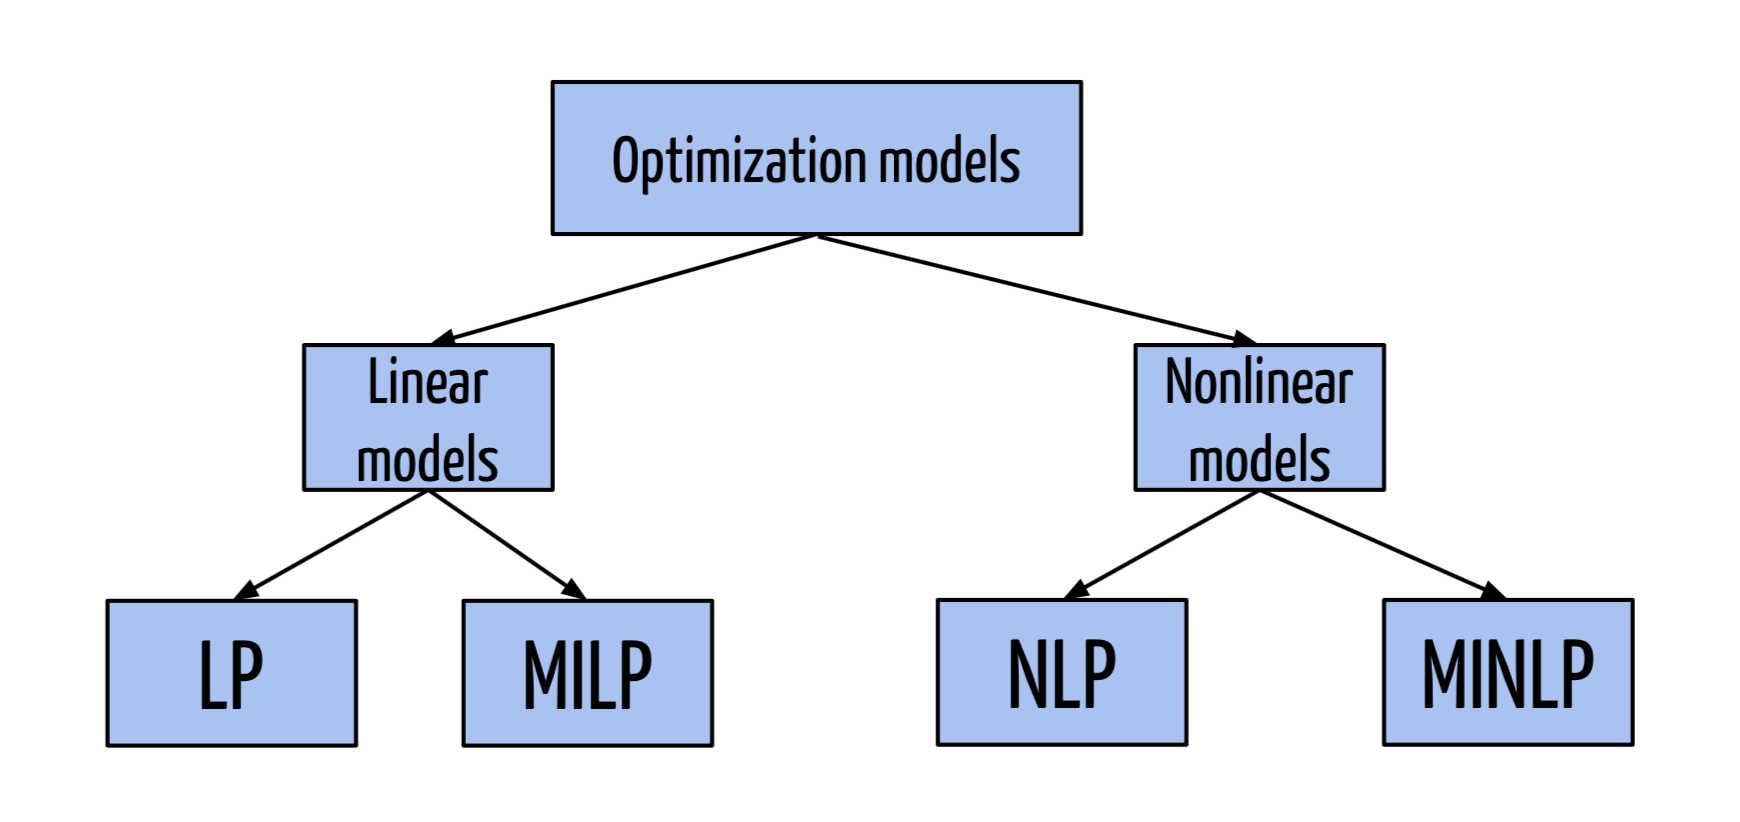
\includegraphics[scale = 0.5]{problem-class-diagram}\footnote{Diagram by Diego Moran}
%\end{center}

\includefigurestatic[][width = 1\linewidth][h]{problem-class-diagram}

Along with each problem class, we will associate a complexity class for the general version of the problem.  See \autoref{sec:complexity} for a discussion of complexity classes.  Although we will often state that input data for a problem comes from $\R$, when we discuss complexity of such a problem, we actually mean that the data is rational, i.e., from $\Q$, and is given in binary encoding.

\section{Linear Programming (LP)}
\todo[inline]{Describe applications and andd images}
Some linear programming background, theory, and examples will be provided in \autoref{sec:LP-background}.
\begin{general}{Linear Programming (LP)}{\polynomial}
%\label{general:LP}
Given a matrix $A \in \R^{m\times n}$, vector $b \in \R^m$ and vector $c \in \R^n$, the \emph{linear programming} problem is
\begin{equation}
\label{eq:LP}
\begin{split}
\max \quad & c^\top x\\
\st  \quad & Ax \leq b\\
& x \geq 0
\end{split}
\end{equation}
\end{general}

Linear programming can come in several forms, whether we are maximizing or minimizing, or if the constraints are $\leq, =$ or $\geq$.   One form commonly used is \emph{Standard Form} given as 
\begin{general}{Linear Programming (LP) Standard Form}{\polynomial}
Given a matrix $A \in \R^{m\times n}$, vector $b \in \R^m$ and vector $c \in \R^n$, the \emph{linear programming} problem in \emph{standard form} is
\begin{equation}
\label{eq:standardLP}
\begin{split}
\max \quad & c^\top x\\
\st  \quad & Ax = b\\
& x \geq 0
\end{split}
\end{equation}
\end{general}
\todo[inline]{Can shrink figure if there are not a lot of numbers of greek letters involved.}
\refincludefigurestatic[Linear programming constraints and objective.][scale = 0.2][h]{wiki/File/linear-programming.png}

\todo[inline]{Move this to simplex chapter}
\begin{exercise}
\label{exercise:LPconversion}
Start with a problem in form given as \eqref{eq:LP} and convert it to standard form \eqref{eq:standardLP} by adding at most $m$ many new variables and by enlarging the constraint matrix $A$ by at most $m$ new columns.
\end{exercise}
\section{Mixed-Integer Linear Programming (MILP)}
Mixed-integer linear programming will be the focus of Sections \ref{sec:IP-formulations},\ref{sec:exponential-IP-forumulations}, \ref{sec:IP-algorithms}, and \ref{sec:IP-heuristics}.
Recall that the notation $\Z$ means the set of integers and the set $\R$ means the set of real numbers.  The first problem of interest here is a \emph{binary integer program} (BIP) where all $n$ variables are binary (either 0 or 1).

\begin{general}{Binary Integer programming (BIP)}{\npcomplete}
Given a matrix $A \in \R^{m\times n}$, vector $b \in \R^m$ and vector $c \in \R^n$, the \emph{binary integer programming} problem is
\begin{equation}
\label{eq:BIP}
\begin{split}
\max \quad & c^\top x\\
\st  \quad & Ax \leq b\\
& x \in \{0,1\}^n
\end{split}
\end{equation}
\end{general}
A slightly more general class is the class of \emph{Integer Linear Programs} (ILP).  Often this is referred to as \emph{Integer Program} (IP), although this term could leave open the possibility of non-linear parts.

\refincludefigurestatic[Comparing the LP relaxation to the IP solutions.][scale = 0.3][h]{wiki/File/integer-programming.png}


\begin{general}{Integer Linear Programming (ILP)}{\npcomplete}
Given a matrix $A \in \R^{m\times n}$, vector $b \in \R^m$ and vector $c \in \R^n$, the \emph{integer linear programming} problem is
\begin{equation}
\label{eq:ILP}
\begin{split}
\max \quad & c^\top x\\
\st  \quad & Ax \leq b\\
& x \in \Z^n
\end{split}
\end{equation}
\end{general}


An even more general class is \emph{Mixed-Integer Linear Programming (MILP)}.  This is where we have $n$ integer variables $x_1, \dots, x_n \in \Z$ and $d$ continuous variables $x_{n+1}, \dots, x_{n+d} \in \R$.  Succinctly, we can write this as $x \in \Z^n \times \R^d$, where $\times$ stands for the \emph{cross-product} between two spaces.   

Below, the matrix $A$ now has $n+d$ columns, that is, $A \in \R^{m \times n+d}$.  Also note that we have not explicitly enforced non-negativity on the variables.  If there are non-negativity restrictions, this can be assumed to be a part of the inequality description $Ax \leq b$.
\begin{general}{Mixed-Integer Linear Programming (MILP)}{\npcomplete}
Given a matrix $A \in \R^{m\times (n+d)}$, vector $b \in \R^m$ and vector $c \in \R^{n+d}$, the \emph{mixed-integer linear programming} problem is
\begin{equation}
\label{eq:ILP}
\begin{split}
\max \quad & c^\top x\\
\st  \quad & Ax \leq b\\
& x \in \Z^n \times \R^d
\end{split}
\end{equation}
\end{general}

\section{Non-Linear Programming (NLP)}
\begin{general}{NLP}{\nphard}
Given a function $f(x)\colon \R^d \to \R$ and other functions $f_i(x)\colon \R^d \to \R$ for $i=1, \dots, m$,  the \emph{nonlinear programming} problem is
\begin{equation}
\label{eq:convex-programming}
\begin{split}
\min \quad & f(x)\\
\st  \quad & f_i(x) \leq 0  \quad  \text{ for } i=1, \dots, m\\
& x \in \R^d
\end{split}
\end{equation}
\end{general}


Nonlinear programming can be separated into convex programming and non-convex programming.  These two are very different beasts and it is important to distinguish between the two.
\subsection{Convex Programming}
Here the functions are all \textbf{convex!}
\begin{general}{Convex Programming}{\polynomial\ \  (typically)}
Given a convex function $f(x)\colon \R^d \to \R$ and convex functions $f_i(x)\colon \R^d \to \R$ for $i=1, \dots, m$,  the \emph{convex programming} problem is
\begin{equation}
\label{eq:convex-programming}
\begin{split}
\min \quad & f(x)\\
\st  \quad & f_i(x) \leq 0  \quad  \text{ for } i=1, \dots, m\\
& x \in \R^d
\end{split}
\end{equation}
\end{general}

Observe that convex programming is a generalization of linear programming.  This can be seen by letting $f(x) = c^\top x$ and $f_i(x) = A_i x - b_i$.  

\subsection{Non-Convex Non-linear Programming}
\todo[inline]{Move this to later chapter on complexity of NLP}
When the function $f$ or functions $f_i$ are non-convex, this becomes a non-convex nonlinear programming problem.  There are a few complexity issues with this.

\paragraph{IP as NLP}
As seen above, quadratic constraints can be used to create a feasible region with discrete solutions.  For example 
$$
x(1-x) = 0
$$
has exactly two solutions: $x = 0, x=1$.  
Thus, quadratic constraints can be used to model binary constraints.
\begin{general}{Binary Integer programming (BIP) as a NLP}{\nphard}
Given a matrix $A \in \R^{m\times n}$, vector $b \in \R^m$ and vector $c \in \R^n$, the \emph{binary integer programming} problem is
\begin{equation}
\label{eq:BIP}
\begin{split}
\max \quad & c^\top x\\
\st  \quad & Ax \leq b\\
& \hcancel[1.5pt]{x \in \{0,1\}^n}\\
& x_i(1-x_i) = 0 \quad \text{ for } i=1, \dots, n
\end{split}
\end{equation}
\end{general}
\subsection{Machine Learning}
\todo[inline]{Many machine learning problems fall into this catrgory.  Todo: describe applications, give references, etc.}
\section{Mixed-Integer Non-Linear Programming (MINLP)}
\todo[inline]{Fill in this section with formulas and discuss applications.  Most notable applications are Electrical Grid problems and Pooling problems. Find applications at Optimization and Engineering \url{https://link.springer.com/journal/11081/volumes-and-issues/21-4}}
\subsection{Convex Mixed-Integer Non-Linear Programming}

\subsection{Non-Convex Mixed-Integer Non-Linear Programming}





%
%
%\end{document}



%%%%%%%%%%%%%%%
%% Comment definition to remove part 1
\def\partOne{Show Part One}
\ifdefined\partOne
%%%%%%%%%%%%%%%%

\part{Linear Programming}
\todo[inline, color = green]{Part I: Linear Programming\\
Notes:  This Part applies to DORI.   We hope for 80\% completion by January 2023, and 100\% completion for January 2024}

\input{optimization/linear-programming-Hildebrand-mix.tex}
%\newcommand\oldstuff{thus}

\section{The Simplex Method} {The Simplex Method}
\todoSection{Integrate this to next chapter (chapter on simplex method)}
\label{lab:Simplex}
\objective{
The \emph{Simplex Method} is a straightforward algorithm for finding optimal solutions to optimization problems with linear constraints and cost functions.
Because of its simplicity and applicability, this algorithm has been named one of the most important algorithms invented within the last 100 years.
In this lab we implement a standard Simplex solver for the primal problem. %s that are feasible at the origin.
}

% The algorithm obtains the solution by traversing the edges of the feasible region defined by the constraints.
% The theory of convex optimization guarantees that the optimal point will be found among the vertices of the feasible region, and so a carefully implemented Simplex Algorithm will discover the exact solution in a finite number of steps.

\subsection*{Standard Form} % ====================================================

The Simplex Algorithm accepts a linear constrained optimization problem, also called a \emph{linear program}, in the form given below:

\begin{align*}
\text{minimize}\qquad &\c\trp\x \\
\text{subject to}\qquad & A\x \leq \b \\
 &\x \geq \0
\end{align*}

Note that any linear program can be converted to standard form, so there is no loss of generality in restricting our attention to this particular formulation.

Such an optimization problem defines a region in space called the \emph{feasible region}, the set of points satisfying the constraints.
Because the constraints are all linear, the feasible region forms a geometric object called a \emph{polytope}, having flat faces and edges (see Figure \ref{fig:polytope}).
The Simplex Algorithm jumps among the vertices of the feasible region searching for an optimal point.
It does this by moving along the edges of the feasible region in such a way that the objective function is always increased after each move.

\begin{figure}[H]
\captionsetup[subfigure]{justification=centering}
\centering
\begin{subfigure}{.5\textwidth} % 2-d feasible polytope.
    \centering
    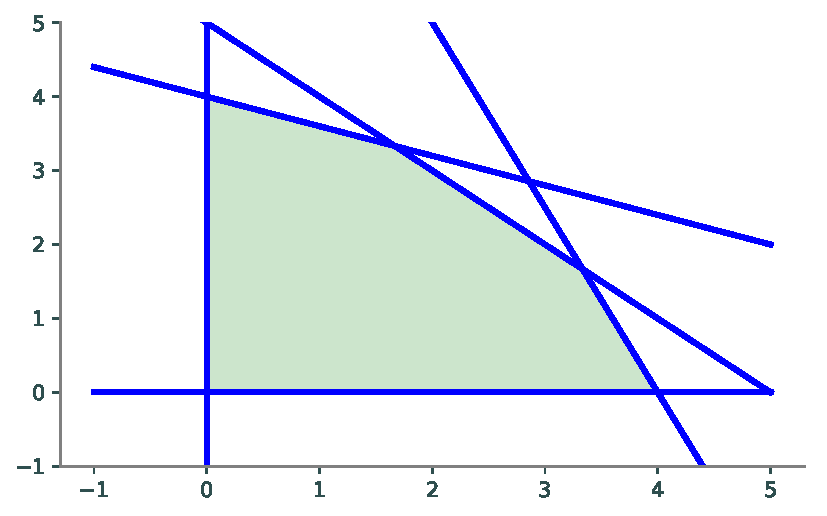
\includegraphics[width=\linewidth]{foundationsAppliedMathematicsLabs/Volume2/Simplex/figures/feasiblePolytope.pdf}
    \caption{The feasible region for a linear program with 2-dimensional constraints.}
\end{subfigure}%
\begin{subfigure}{.5\textwidth} % 3-d feasible polytope.
    \begin{center}
    \begin{tikzpicture}[dot/.style={circle,fill=blue,minimum size=3pt,inner sep=0pt, outer sep=-1pt}, >=stealth']

    \draw[blue!10!, fill=blue!5!](3,1)--(1.5,2.3)--(1.75,1.3)--cycle;
    \draw[blue!25!, fill = blue!15!](3,1)--(1.75,1.3)--(2.3,-1)--cycle;
    \draw[blue!55!, fill = blue!40!](1.75,1.3)--(2.3,-1)--(.8,-1)--cycle;
    \draw[blue!80!, fill = blue!65!](.8,-1)--(-.05,-.2)--(.25,.6)--(1.22,.06)--cycle;
    \draw[blue!85!, fill = blue!73!](-.05, -.2)--(-.3,0)--(.1, 1.65)--(.25, .6)--cycle;
    \draw[blue!65!, fill = blue!50!](.1,1.7)--(.25,.6)--(1.22,.07)--(1.75,1.3)--cycle;
    \draw[blue!40!, fill = blue!15!](.1,1.7)--(1.75,1.3)--(1.5,2.3)--cycle;

    \draw[-,thick](-.3,0)--(.1,1.7)--(1.5, 2.3)--(3, 1)--(2.3,-1)--(.8,-1)--cycle;

    \draw[-,thick](.1,1.7)--(3,1);
    \draw[-,thick](1.5, 2.3)--(2.3,-1);
    \draw[-,thick](.8,-1)--(1.74,1.3);
    \draw[-,thick](.1,1.7)--(.25,.6);
    \draw[-,thick](1.24,.07)--(.25,.6);
    \draw[-,thick](-.05,-.24)--(.25,.6);

    \draw[->](.37,.63)--(.22,1.61);
    \draw[->](.31,1.55)--(1.63,1.23);
    \draw[->](.75,-.85)--(1.12,.05);
    \draw[->](1.05,.05)--(.25,.48);
    \draw[->](1.83,1.35)--(1.65,2.1);

    \node[draw=none](x*)at(1.8,2.45){$\x^*$};

    \end{tikzpicture}
    \end{center}
    \caption{The feasible region for a linear program with 3-dimensional constraints.}
\end{subfigure}
\caption{If an optimal point exists, it is one of the vertices of the polyhedron.
The simplex algorithm searches for optimal points by moving between adjacent vertices in a direction that increases the value of the objective function until it finds an optimal vertex.}
\label{fig:polytope}
\end{figure}

% \begin{figure}[htb] % 3-d feasible polytope.
% \end{figure}


% % TODO: subfigure for 3-d polytope from book.

Implementing the Simplex Algorithm is straightforward, provided one carefully follows the procedure.
We will break the algorithm into several small steps, and write a function to perform each one.
To become familiar with the execution of the Simplex algorithm, it is helpful to work several examples by hand.

\subsection*{The Simplex Solver} % ===============================================

Our program will be more lengthy than many other lab exercises and will consist of a collection of functions working together to produce a final result.
It is important to clearly define the task of each function and how all the functions will work together.
If this program is written haphazardly, it will be much longer and more difficult to read than it needs to be.
We will walk you through the steps of implementing the Simplex Algorithm as a Python class.
% Since the Simplex Algorithm assumes that all the variables are non-negative, we do not need any special logic for it.
% what is this previous statement saying? What 'special logic' would you need if the variables were negative?

For demonstration purposes, we will use the following linear program.
\begin{align*}
\text{minimize}\qquad & -3x_0 - 2x_1 \\
\text{subject to}\qquad
& x_0 - x_1 \leq 2 \\
& 3x_0 + x_1 \leq 5 \\
& 4x_0 + 3x_1 \leq 7 \\
& x_0, x_1 \geq 0.
\end{align*}

\subsection*{Accepting a Linear Program} % ------------------------------------

Our first task is to determine if we can even use the Simplex algorithm.
Assuming that the problem is presented to us in standard form, we need to check that the feasible region includes the origin.  For now, we only check for feasibility at the origin. A more robust solver sets up the auxiliary problem and solves it to find a starting point if the origin is infeasible.

\begin{problem}{Check feasibility at the origin.}{}
Write a class that accepts the arrays $\c$, $A$, and $\b$ of a linear optimization problem in standard form.
In the constructor, check that the system is feasible at the origin.
That is, check that $A\x \preceq \b$ when $\x = \0$. Raise a \li{ValueError} if the problem is not feasible at the origin. \label{prob:initsolver}
\end{problem}

\subsection*{Adding Slack Variables} % ----------------------------------------

The next step is to convert the inequality constraints $A\x \leq \b$ into equality constraints by introducing a slack variable for each constraint equation.
If the constraint matrix $A$ is an $m \times n$ matrix, then there are $m$ slack variables, one for each row of $A$.
Grouping all of the slack variables into a vector $\w$ of length $m$, the constraints now take the form $A\x + \w = \b$.
In our example, we have \[\w = \left[\begin{array}{c}x_2\\x_3 \\x_4\end{array}\right]\]

% TODO: change the representation of the slack variables to match the book.
When adding slack variables, it is useful to represent all of your variables, both the original primal variables and the additional slack variables, in a convenient manner.
One effective way is to refer to a variable by its subscript.
For example, we can use the integers $0$ through $n-1$ to refer to the original (non-slack) variables $x_0$ through $x_{n-1}$, and we can use the integers $n$ through $n+m-1$ to track the slack variables (where the slack variable corresponding to the $i$th row of the constraint matrix is represented by the index $n+i-1$).

We also need some way to track which variables are \emph{independent} (non-zero) and which variables are \emph{dependent} (those that have value $0$). This can be done using the objective function. At anytime during the optimization process, the non-zero variables in the objective function are \emph{independent} and all other variables are \emph{dependent}. 

%A useful representation for the variables is a Python list (or NumPy array), where the elements of the list are integers.
%Since we know how many dependent variables we have ($m$), we can partition the list so that all the dependent variables are kept in the first $m$ locations, and all the independent variables are stored at the end of the list.
%The ordering of this list is important.
%In particular, if $i \leq m$, the $i$th element of the list represents the dependent variable corresponding to the $i$th row of $A$.
%Henceforth we will refer to this list as the \emph{index list}.

%Initially, the dependent variables are simply the slack variables, and their values correspond to the values of %the vector $\b$.
%In our example, we have 2 primal variables $x_0$ and $x_1$, and we must add 3 slack variables.
%Thus, we instantiate the following index list:

%\begin{lstlisting}
%>>> L = [2, 3, 4, 0, 1]
%\end{lstlisting}

%Notice how the first $3$ entries of the index list are $2, 3, 4$, the indices representing the slack variables.
%This reflects the fact that the dependent variables at this point are exactly the slack variables.

%As the Simplex Algorithm progresses, however, the dependent variables change, and it will be necessary to swap
%elements in our index list.
%For example, suppose the variable represented by the index $4$ becomes independent, while the variable %represented by index $0$ becomes dependent.
%In this case we swap these two entries in the index list.

%\begin{lstlisting}
%>>> L[2], L[3] = L[3], L[2]
%>>> L
%[2, 3, 0, 4, 1]
%\end{lstlisting}

%Now our index list tells us that the current dependent variables $2, 3, 0$.

%\begin{problem} % Slack variables. % TODO: this problem is worthless...
%Design and implement a way to store and track all of the dependent and independent variables.

%Hint: Using integers that represent the index of each variable is useful for Problem \ref{prob:blands}.
%\label{prob:slackvars}
%\end{problem}

\subsection*{Creating a Dictionary} % --------------------------------------------

After we have determined that our program is feasible, we need to create the \emph{dictionary} (sometimes called the \emph{tableau}), a matrix to track the state of the algorithm.
%Remember that your dictionary will need to include in some way the slack variables that you created in Problem \ref{prob:slackvars}.

There are many different ways to build your dictionary.
One way is to mimic the dictionary that is often used when performing the Simplex Algorithm by hand. To do this we will set the corresponding dependent variable equations to 0. For example, if $x_5$ were a dependent variable we would expect to see a -1 in the column that represents $x_5$.
Define \[\bar{A} = \left[\begin{array}{cc} A & I_m \end{array}\right],\]
where $I_m$ is the $m \times m$ identity matrix we will use to represent our slack variables, and define
\[\bar{\c} = \left[\begin{array}{c}\c\\ \0\end{array}\right].\]
That is, $\bar{\c} \in \mathbb{R}^{n+m}$ such that the first $n$ entries are $\c$ and the final $m$ entries are zeros.
Then the initial dictionary has the form
\begin{equation}
D =
\left[\begin{array}{ccc}
0  & \bar{\c}\trp \\
\b &  -\bar{A} 
\end{array}\right]
\label{eqn:hand_tab}
\end{equation}

The columns of the dictionary correspond to each of the variables (both primal and slack), and the rows of the dictionary correspond to the dependent variables.
%Using the convention introduced above of representing the variables by indices in the index list, we have the following correspondence:
%\[
%\text{column } i \Leftrightarrow \text{index } i-2, \qquad i = 2, 3, \ldots, n+m+1,
%\]
%and
%\[
%\text{row } j \Leftrightarrow L_{j-1}, \qquad j = 2, 3, \ldots, m+1,
%\]
%where $L_{j-1}$ refers to the $(j-1)$th entry of the index list.

%For our example problem, the initial index list is
%\[
%L = (2, 3, 4, 0, 1),
%\]
For our example the initial dictionary is
\begin{equation*}
D = \begin{bmatrix}
    0 & -3 & -2 & 0 & 0 & 0\\
    2 & -1 & 1 & -1 & 0 & 0\\
    5 & -3 & -1 & 0 & -1 & 0\\
    7 & -4 & -3 & 0 & 0 & -1
    \end{bmatrix}.
\end{equation*}
%The third column corresponds to index $1$, and the fourth row corresponds to index $4$, since this is the
%third entry of the index list.

The advantage of using this kind of dictionary is that it is easy to check the progress of your algorithm by hand.
%The disadvantage is that pivot operations require careful bookkeeping to track the variables and constraints.

% This dictionary is less intuitive, and I think could lead to more confusion.
\begin{comment}
We can also use a dictionary of the format:
\begin{equation}
T = \begin{bmatrix}
    0 & \c\trp  & 0 \\
    \0 & I_n & \0\\
    \b & -A  & \0
\end{bmatrix}.
\label{eqn:matrix_tab}
\end{equation}
Here, $T$ is a square matrix of size $(n+m+1) \times (n+m+1)$.
The advantage of this form of the dictionary is that all the pivot bookkeeping is built into the matrix.
For our example problem, the initial dictionary of this form is
\begin{equation}
T = \begin{bmatrix}
        0 & 3 & 2 & 0 & 0 & 0 \\
        0 & 1 & 0 & 0 & 0 & 0 \\
        0 & 0 & 1 & 0 & 0 & 0 \\
        2 &-1 & 1 & 0 & 0 & 0 \\
        5 &-3 &-1 & 0 & 0 & 0 \\
        7 &-4 &-3 & 0 & 0 & 0
\end{bmatrix}.
\label{eqn:matrix_inittab}
\end{equation}
\end{comment}

\begin{problem}{Initialize the dictionary.}
Add a method to your Simplex solver that takes in arrays c, A, and b to create the initial dictionary (D) as a NumPy array.
\label{prob:makedictionary}
\end{problem}

\subsection{Pivoting} % ------------------------------------------------------

Pivoting is the mechanism that really makes Simplex useful.
Pivoting refers to the act of swapping dependent and independent variables, and transforming the dictionary appropriately.
This has the effect of moving from one vertex of the feasible polytope to another vertex in a way that increases the value of the objective function.
Depending on how you store your variables, you may need to modify a few different parts of your solver to reflect this swapping.

When initiating a pivot, you need to determine which variables will be swapped.
In the dictionary representation, you first find a specific element on which to pivot, and the row and column that contain the pivot element correspond to the variables that need to be swapped.
Row operations are then performed on the dictionary so that the pivot column becomes a negative elementary vector.

Let's break it down, starting with the pivot selection.
We need to use some care when choosing the pivot element.
To find the pivot column, search from left to right along the top row of the dictionary (ignoring the first column), and stop once you encounter the first negative value.
The index corresponding to this column will be designated the \emph{entering index}, since after the full pivot operation, it will enter
the basis and become a dependent variable.

Using our initial dictionary $D$ in the example, we stop at the second column:
\[ D = \left[ \:
\begin{array}{*{7}{c}}
\cline{2-2}
0 & \multicolumn{1}{|c}{-3} & \multicolumn{1}{|c}{-2} & 0 & 0 & 0\\
2 & \multicolumn{1}{|c}{-1} & \multicolumn{1}{|c}{1} & -1 & 0 & 0\\
5 & \multicolumn{1}{|c}{-3} & \multicolumn{1}{|c}{-1} & 0 & -1 & 0\\
7 & \multicolumn{1}{|c}{-4} & \multicolumn{1}{|c}{-3} & 0 & 0 & -1\\
\cline{2-2}
\end{array}
\right] \]
We now know that our pivot element will be found in the second column.
The entering index is thus $1$.

Next, we select the pivot element from among the negative entries in the pivot column (ignoring the entry in the first row).
\emph{If all entries in the pivot column are non-negative, the problem is unbounded and has no solution.}
In this case, the algorithm should terminate.
Otherwise, assuming our pivot column is the $j$th column of the dictionary and that the negative entries of this column are
$D_{i_1, j}, D_{i_2, j}, \ldots, D_{i_k, j}$, we calculate the ratios
\[
\frac{-D_{i_1,0}}{D_{i_1,j}}, \frac{-D_{i_2,0}}{D_{i_2,j}}, \ldots, \frac{-D_{i_k,0}}{D_{i_k,j}},
\]
and we choose our pivot element to be one that minimizes this ratio.
If multiple entries minimize the ratio, then we utilize \emph{Bland's Rule}, which instructs us to choose the entry in the row corresponding to the smallest index (obeying this rule is important, as it prevents the possibility of the algorithm cycling back on itself infinitely).
The index corresponding to the pivot row is designated as the \emph{leaving index}, since after the full pivot operation, it will leave the basis and become a independent variable.

In our example, we see that all entries in the pivot column (ignoring the entry in the first row, of course) are negative, and hence they are all potential choices for the pivot element.
We then calculate the ratios, and obtain
\[
\frac{-2}{-1} = 2,\quad \frac{-5}{-3} = 1.66...,\quad \frac{-7}{-4} = 1.75.
\]
We see that the entry in the third row minimizes these ratios.
Hence, the element in the second column (index 1), third row (index 2) is our designated
pivot element.

\[ D = \left[ \:
\begin{array}{*{7}{c}}

0 & -3 & -2 & 0 & 0 & 0\\
2 & -1 & 1 & -1 & 0 & 0\\\cline{2-2}
5 & \multicolumn{1}{|c}{-3} & \multicolumn{1}{|c}{-1} & 0 & -1 & 0\\\cline{2-2}
7 & -4 & -3 & 0 & 0 & -1\\
\end{array}
\right] \]

\begin{comment}
If we are using the dictionary representation in equation \ref{eqn:matrix_tab}, pivot operations are reduced to a simple matrix equation:
\[T = T + T_m \otimes T_n,\]
where $T_m$ is the column corresponding to the variable entering the basis and $T_n$ is a normalized vector corresponding to the variable leaving the basis.
The result of the equation is the new dictionary.

For example, for the initial dictionary, \ref{eqn:matrix_inittab}, we will demonstrate the first pivot operation.
We can do the entire pivot with a single outer product.
The first pivot should occur with $x_1$ leaving and $x_4$ entering.
In other words, we want to pivot at row $i = 4$ and column $j = 1$ in the dictionary (the indices are offset by one because of the objective function and the row of constraints).

The row corresponding to $x_4$ is
\[
\begin{bmatrix} 5 &-3 &-1 & 0 & 0 & 0\end{bmatrix}.
\]
This represents the equation
\[
x_4 = 5 - 3x_1 - x_2.
\]
Our eventual goal is to solve for $x_1$ and substitute into the remaining rows of the dictionary.
A simple method to accomplish this is to rewrite the equation so that we have zero on the left-hand side:
\[
0 = 5 - 3x_1 - x_2 - x_4.
\]
Now, we can normalize this equation so that the coefficient of $x_1$ is $-1$.
This is always accomplished by dividing the equation by the negative of the coefficient of $x_1$:
\begin{equation}
0 = \frac{5}{3} - x_1 - \frac{1}{3}x_2 - \frac{1}{3}x_4.
\label{eq:zero-equation}
\end{equation}
This is represented by the vector
\[
\begin{bmatrix} 5/3 & -1 & -1/3 & 0 & -1/3 & 0\end{bmatrix}.
\]
Since this left-hand side is zero, I can add any scalar multiple of this equation to any of the equations for $x_i$ and still have an equation for $x_i$.
For example, the equation for $x_5$ is
\[
x_5 = 7 - 4x_1 - 3x_2.
\]
Thus, I can add $-4$ times \eqref{eq:zero-equation} to this equation without changing the left-hand side:
\[ x_5 = 7 - 4x_1 - 3x_2 = 7 - 4x_1 - 3x_2 + -4\left(\frac{5}{3} - x_1 - \frac{1}{3}x_2 - \frac{1}{3}x_4\right) = \frac{1}{3} - \frac{5}{3}x_2 + \frac{4}{3} x_4.
\]
Notice that we end up with an equation that does not include $x_1$ and now has $x_4$, just like we wanted.
In fact, this works in all of our equations, including those for the objective function and even for $x_1$!
Since the coefficient of $x_1$ in \eqref{eq:zero-equation} is $-1$, when we scale it by the coefficient of $x_1$ in any particular row, the $x_1$ cancels out.
\[
T = T + \begin{bmatrix}3 \\ 1 \\ 0 \\ -1 \\ -3 \\ -4\end{bmatrix}\begin{bmatrix} 5/3 & -1 & -1/3 & 0 & -1/3 & 0\end{bmatrix}.
\]
The column vector is just the second column of $T$, which is the column containing the coefficients of $x_1$ in each row.
When we compute this sum, we obtain the dictionary.
\[
T = \begin{bmatrix}
        5 &  0 & 1 & 0 & -1 & 0 \\
        5/3 & 0 &-1/3 & 0 &-1/3 & 0 \\
        0 & 0 & 1 & 0 & 0 & 0 \\
        1/3 & 0 & 4/3 & 0 & 1/3 & 0 \\
        0 & 0 & 0 & 0 & 1 & 0 \\
        1/3 & 0 & -5/3 & 0 & 4/3 & 0
\end{bmatrix}.
\]
\end{comment}
%\begin{problem}
%Write a method that will determine the pivot row and pivot column according to Bland's Rule.
% \begin{comment}
\begin{definition}{Bland's Rule}
Choose the independent variable with the smallest index that has a negative coefficient in the objective function
as the leaving variable.
Choose the dependent variable with the smallest index among all the binding dependent variables.
\end{definition}

Bland's Rule is important in avoiding cycles when performing pivots.
This rule guarantees that a feasible Simplex problem will terminate in a finite number of pivots.% \emph{Hint:} Avoid dividing by zero.
% \end{comment}
%\label{prob:blands}
%\end{problem}

%The next step is to swap the entering and leaving indices in our index list.
%In the example, we determined above that these indices are $0$ and $3$.
%We swap these two elements in our index list,
%and the updated index list is now
%\[
%L = (2, 0, 4, 3, 1),
%\]
%so the dependent variables are now given by the indices $2, 0, 4$.

Finally, we perform row operations on our dictionary in the following way: divide the pivot row by the negative value of the pivot entry.
Then use the pivot row to zero out all entries in the pivot column above and below the pivot entry.
In our example, we first divide the pivot row by -3, and then zero out the two entries above the pivot element and the single entry below it:
\begin{align*}
\begin{bmatrix}
    0 & -3 & -2 & 0 & 0 & 0\\
    2 & -1 & 1 & -1 & 0 & 0\\
    5 & -3 & -1 & 0 & -1 & 0\\
    7 & -4 & -3 & 0 & 0 & -1
    \end{bmatrix} &\rightarrow
\begin{bmatrix}
    0 & -3 & -2 & 0 & 0 & 0\\
    2 & -1 & 1 & -1 & 0 & 0\\
    5/3 & -1 & -1/3 & 0 & -1/3 & 0\\
    7 & -4 & -3 & 0 & 0 & -1
    \end{bmatrix}\rightarrow\\
\begin{bmatrix}
    -5 & 0 & -1 & 0 & 1 & 0\\
    2 & -1 & 1 & -1 & 0 & 0\\
    5/3 & -1 & -1/3 & 0 & -1/3 & 0\\
    7 & -4 & -3 & 0 & 0 & -1
    \end{bmatrix} &\rightarrow
\begin{bmatrix}
    -5 & 0 & -1 & 0 & 1 & 0\\
    1/3 & 0 & -4/3 & 1 & -1/3 & 0\\
    5/3 & -1 & -1/3 & 0 & -1/3 & 0\\
    7 & -4 & -3 & 0 & 0 & -1
    \end{bmatrix}\rightarrow\\
\begin{bmatrix}
    -5 & 0 & -1 & 0 & 1 & 0\\
    1/3 & 0 & 4/3 & -1 & 1/3 & 0\\
    5/3 & -1 & -1/3 & 0 & -1/3 & 0\\
    1/3 & 0 & -5/3 & 0 & 4/3 & -1
    \end{bmatrix}&.
\end{align*}
The result of these row operations is our updated dictionary, and the pivot operation is complete.

\begin{problem}{Pivoting}
Add a method to your solver that checks for unboundedness and performs a single pivot operation from start to completion.
If the problem is unbounded, raise a \li{ValueError}.
\end{problem}

\vspace{2mm}

\subsection{Termination and Reading the Dictionary} % ---------------------------

Up to this point, our algorithm accepts a linear program, adds slack variables, and creates the initial dictionary.
After carrying out these initial steps, it then performs the pivoting operation iteratively until the optimal point is found.
But how do we determine when the optimal point is found? The answer is to look at the top row of the dictionary, which represents the objective function.
More specifically, before each pivoting operation, check whether all of the entries in the top row of the dictionary (ignoring the entry in the first column) are nonnegative.
If this is the case, then we have found an optimal solution, and so we terminate the algorithm.

The final step is to report the solution.
The ending state of the dictionary and index list tells us everything we need to know.
The minimal value attained by the objective function is found in the upper leftmost entry of the dictionary.
The dependent variables all have the value $0$ in the objective function or first row of our dictionary array. The independent variables have values given by the first column of the dictionary.
Specifically, the independent variable whose index is located at the $i$th entry of the index list has the value $T_{i+1, 0}$.

In our example, suppose that our algorithm terminates with the dictionary and index list in the following state:
\[
D = \begin{bmatrix}
-5.2 & 0 & 0 & 0 & 0.2 & 0.6\\
0.6 & 0 & 0 & -1 & 1.4 & -0.8\\
1.6 & -1 & 0 & 0 & -0.6 & 0.2\\
0.2 & 0 & -1 & 0 & 0.8 & -0.6\\
\end{bmatrix}
\]
%\[
%L = (2, 0, 1, 3, 4).
%\]
Then the minimal value of the objective function is $-5.2$.
The independent variables have indices $4, 5$ and have the value $0$.
The dependent variables have indices $3, 1,$ and $2$, and have values $.6, 1.6$, and $.2$, respectively.
In the notation of the original problem statement, the solution is given by
\begin{align*}
x_0 &= 1.6\\
x_1 &= .2.
\end{align*}

\begin{problem}{SimplexSolver.solve()}
Write an additional method in your solver called \li{solve()} that obtains the optimal solution, then returns the minimal value, the dependent variables, and the independent variables.
The dependent and independent variables should be represented as two dictionaries that map the index of the variable to its corresponding value.

For our example, we would return the tuple 

\li{(-5.2, \{0: 1.6, 1: .2, 2: .6\}, \{3: 0, 4: 0\})}.
%The correct format of this tuple is critical, as this tuple of information will be used judge whether or not your solver works!
\end{problem}

\vspace{5mm}

At this point, you should have a Simplex solver that is ready to use.
The following code demonstrates how your solver is expected to behave:

\vspace{5mm}

\begin{lstlisting}
>>> import SimplexSolver

# Initialize objective function and constraints.
>>> c = np.array([-3., -2.])
>>> b = np.array([2., 5, 7])
>>> A = np.array([[1., -1], [3, 1], [4, 3]])

# Instantiate the simplex solver, then solve the problem.
>>> solver = SimplexSolver(c, A, b)
>>> sol = solver.solve()
>>> print(sol)
(-5.2,
 {0: 1.6, 1: 0.2, 2: 0.6},
 {3: 0, 4: 0})
\end{lstlisting}

If the linear program were infeasible at the origin or unbounded, we would expect the solver to alert the user by raising an error.

Note that this simplex solver is \emph{not} fully operational.
It can't handle the case of infeasibility at the origin.
This can be fixed by adding methods to your class that solve the \emph{auxiliary problem}, that of finding an initial feasible dictionary when the problem is not feasible at the origin.
Solving the auxiliary problem involves pivoting operations identical to those you have already implemented, so adding this functionality
is not overly difficult.


\subsection{Exercises}

\paragraph{Exercise $1.0$ (Learn $\mathrm{LT}_{\mathrm{E}} \mathrm{X}$ )}

Learn to use $\operatorname{lt}_{\mathrm{E}} X$ for writing all of your homework solutions. Personally, I use MiKTEX, which is an implementation of $\mathrm{ET} \mathrm{E} \mathrm{X}$ for Windows. Specifically, within MiKTEX I am using pdfteTEX (it only matters for certain things like including graphics and also pdf into a document). I find it convenient to use the editor WinEdt, which is very LATEX friendly. A good book on $\mathrm{ET} \mathrm{T} \mathrm{X}$ is

In A.1 there is a template to get started. Also, there are plenty of tutorials and beginner's guides on the web.

\paragraph{Exercise $1.1$ (Convert to standard form)}

Give an original example (i.e., with actual numbers) to demonstrate that you know how to transform a general linear-optimization problem to one in standard form.

\paragraph{Exercise $1.2$ (Weak Duality example)}

Give an original example to demonstrate the Weak Duality Theorem.

\paragraph{Exercise $1.3$ (Convert to $\leq$ form)}

Describe a general recipe for transforming an arbitrary linear-optimization problem into one in which all of the linear constraints are of $\leq$ type.

\paragraph{Exercise $1.4$ ( $m+1$ inequalities)}

Prove that the system of $m$ equations in $n$ variables $A x=b$ is equivalent to the system $A x \leq b$ augmented by only one additional linear inequality - that is, a total of only $m+1$ inequalities.

\paragraph{Exercise $1.5$ (Weak duality for another form)}

Give and prove a Weak Duality Theorem for

$$
\begin{aligned}
\max \quad c^{\prime} x & \\
A x & \leq b ; \\
x & \geq 0 .
\end{aligned}
$$

HINT: Convert $\left(\mathrm{P}^{\prime}\right)$ to a standard-form problem, and then apply the ordinary Weak Duality Theorem for standard-form problems. \paragraph{Exercise 1.6 (Weak duality for a complicated form)}

Give and prove a Weak Duality Theorem for

$$
\begin{gathered}
\min \quad c^{\prime} x+f^{\prime} w \\
\begin{aligned}
A x+B w & \leq b ; \\
D x &=g ;
\end{aligned} \\
x \geq 0 \quad w \leq 0
\end{gathered}
$$

HINT: Convert $\left(\mathrm{P}^{\prime}\right)$ to a standard-form problem, and then apply the ordinary Weak Duality Theorem for standard-form problems.

\paragraph{Exercise $1.7$ (Weak duality for a complicated form - with MATLAB)}

The MATLAB code below makes and solves an instance of $\left(\mathrm{P}^{\prime}\right)$ from Exercise 1.6. Study the code to see how it is works. Now, extend the code to solve the dual of $\left(\mathrm{P}^{\prime}\right)$. Also, after converting $\left(\mathrm{P}^{\prime}\right)$ to standard form (as indicated in the HINT for Exercise 1.6), use MATLAB to solve that problem and its dual. Make sure that you get the same optimal value for all of these problems.





\subsection{$2.5$ Exercises}

\paragraph{Exercise 2.1 (Dual in AMPL)}

Without changing the file production. dat, use AMPL to solve the dual of the Production Problem example, as described in Section 2.1. You will need to modify production.mod and production.run.

\paragraph{Exercise $2.2$ (Sparse solution for linear equations with AMPL)}

In some application areas, it is interesting to find a "sparse solution" - that is, one with few non-zeros - to a system of equations $A x=b$. It is well known that a 1-norm minimizing solution is a good heuristic for finding a sparse solution. Using AMPL, try this idea out on several large examples, and report on your results.

HINT: To get an interesting example, try generating a random $m \times n$ matrix $A$ of zeros and ones, perhaps $m=50$ equations and $n=500$ variables, maybe with probability $1 / 2$ of an entry being equal to one. Then choose maybe $m / 2$ columns from $A$ and add them up to get $b$. In this way, you will know that there is a solution with only $m / 2$ non-zeros (which is already pretty sparse). Your 1-norm minimizing solution might in fact recover this solution $(\odot)$, or it may be sparser $(\odot \odot)$, or perhaps less sparse $(\odot)$.

\paragraph{Exercise $2.3$ (Bloody AMPL)}

A transportation problem is a special kind of (single-commodity min-cost) networkflow problem. There are certain nodes $v$ called supply nodes which have net supply $b_{v}>0$. The other nodes $v$ are called demand nodes, and they have net supply $b_{v}<0$. There are no nodes with $b_{v}=0$, and all arcs point from supply nodes to demand nodes.

A simplified example is for matching available supply and demand of blood, in types $A, B, A B$ and $O$. Suppose that we have $s_{v}$ units of blood available, in types $v \in\{A, B, A B, O\}$. Also, we have requirements $d_{v}$ by patients of different types $v \in$ $\{A, B, A B, O\}$. It is very important to understand that a patient of a certain type can accept blood not just from their own type. Do some research to find out the compatible blood types for a patient; don't make a mistake - lives depend on this! In this spirit, if your model misallocates any blood in an incompatible fashion, you will receive a grade of $F$ on this problem.

Describe a linear-optimization problem that satisfies all of the patient demand with compatible blood. You will find that type $O$ is the most versatile blood, then both $A$ and $B$, followed by $A B$. Factor in this point when you formulate your objective function, with the idea of having the left-over supply of blood being as versatile as possible.

Using AMPL, set up and solve an example of a blood-distribution problem.

\paragraph{Exercise $2.4$ (Mix it up)}

"I might sing a gospel song in Arabic or do something in Hebrew. I want to mix it up and do it differently than one might imagine." - Stevie Wonder

We are given a set of ingredients $1,2, \ldots, m$ with availabilities $b_{i}$ and per unit costs $c_{i}$. We are given a set of products $j, 2, \ldots, m$ with minimum production requirements $d_{j}$ and per unit revenues $e_{j}$. It is required that product $j$ have at least a fraction of $l_{i j}$ of ingredient $i$ and at most a fraction of $u_{i j}$ of ingredient $i$. The goal is to devise a plan to maximize net profit.

Formulate, mathematically, as a linear-optimization problem. Then, model with AMPL, make up some data, try some computations, and report on your results. Exercise $2.5$ (Task scheduling)


We are given a set of tasks, numbered $1,2, \ldots, n$ that should be completed in the minimum amount of time. For convenience, task 0 is a "start task" and task $n+1$ is an "end task". Each task, except for the start and end task, has a known duration $d_{i}$. For convenience, let $d_{0}:=0$. There are precedences between tasks. Specifically, $\Psi_{i}$ is the set of tasks that must be completed before task $i$ can be started. Let $t_{0}:=0$, and for all other tasks $i$, let $t_{i}$ be a decision variable representing its start time.

Formulate the problem, mathematically, as a linear-optimization problem. The objective should be to minimize the start time $t_{n+1}$ of the end task. Then, model the problem with AMPL, make up some data, try some computations, and report on your results.

\paragraph{Exercise $2.6$ (Investing wisely)}

Almost certainly, Albert Einstein did not say that "compound interest is the most powerful force in the universe."

A company wants to maximize their cash holdings after $T$ time periods. They have an external inflow of $p_{t}$ dollars at the start of time period $t$, for $t=1,2, \ldots, T$. At the start of each time period, available cash can be allocated to any of $K$ different investment vehicles (in any available non-negative amounts). Money allocated to investmentvehicle $k$ at the start of period $t$ must be held in that investment $k$ for all remaining time periods, and it generates income $v_{t, t}^{k}, v_{t, t+1}^{k}, \ldots, v_{t T}^{k}$, per dollar invested. It should be assumed that money obtained from cashing out the investment at the end of the planning horizon (that is, at the end of period $T$ ) is part of $v_{t, T}^{k}$. Note that at the start of time period $t$, the cash available is the external inflow of $p_{t}$, plus cash accumulated from all investment vehicles in prior periods that was not reinvested. Finally, assume that cash held over for one time period earns interest of $q$ percent.

Formulate the problem, mathematically, as a linear-optimization problem. Then, model the problem with AMPL, make up some data, try some computations, and report on your results.






\chapter{Simplex Method}

\todoChapter{{\color{gray}10\% complete. Goal 80\% completion date: January 20, 2023}\\
Notes: This section hasn't been cleaned at all.  This needs to be looked at and cleaned up.}

\begin{definition}{Standard Form}{standardform}
A linear program is in \emph{standard form} if is written as 
\begin{align*}
\max \ \ &c^\top x \\
s.t. \ \ & Ax = b\\
& x \geq 0.
\end{align*}
\end{definition}

\begin{definition}{Extreme Point}{extremepoint}
A point $x$ in a convex set $C$ is called an \emph{extreme point} if it cannot be written as a strict convex combination of other points in $C$.
\end{definition}

\begin{theorem}{Optimal Extreme Point - Bounded Case}{}
Consider a linear optimization problem in standard form.  Suppose that the feasible region is bounded and non-empty. 

Then there exists an optimal solution at an extreme point of the feasible region.
\end{theorem}

\begin{proof}[Proof Sketch]

\end{proof}


% Winston
\begin{definition}{Basic solution}{}
A basic solution to $Ax = b$ is obtained by setting $n-m$ variables equal to $0$ and solving for the values of the remaining $m$ variables.  This assumes that the setting $n-m$ variables equal to 0 yields unique values for the remaining $m$ variables or, equivalently, the columns of the remaining $m$ variables are linearly independent.
\end{definition}

\begin{example}{}{}
Consider the problem
\begin{align*}
\max \quad & Z =-5 X-7 Y  \\ 
\text { s.t. } \quad & X+3 Y \geq 6 \\ 
&5 X+ 2 Y \geq 10 \\ 
&Y  \leq 4 \\ 
&X, Y  \geq 0 
\end{align*}

\begin{center}
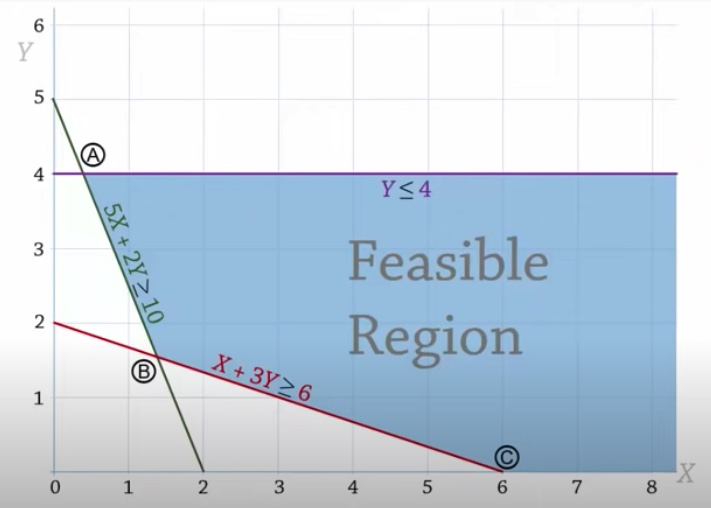
\includegraphics[scale = 0.4]{screenshots/example1-feasible-region}
\end{center}

We begin by converting this problem to standard form.  
\begin{align*}
\max \quad & Z =-5 X-7 Y + 0s_1 + 0s_2 + 0 s_3\\ 
\text { s.t. } \quad & X+3 Y - s_1 = 6 \\ 
&5 X+ 2 Y - s_2 = 10 \\ 
&Y  + s_3 = 4 \\ 
&X, Y, s_1, s_2, s_3  \geq 0 
\end{align*}

Thus, we can write this problem in matrix form with 

\begin{align}
\max  & \begin{bmatrix}
-5 \\ -7 \\ 0 \\ 0 \\0
\end{bmatrix}^\top \begin{bmatrix}
X\\Y\\s_1\\s_2\\ s_3
\end{bmatrix}\\
&\begin{bmatrix}
1 & 3 & -1 & 0 & 0 \\
5 & 2 & 0 & -1 & 0\\
0 & 1 & 0 & 0 & 1\\
\end{bmatrix}
\begin{bmatrix}
X \\ Y \\ s_1 \\ s_2 \\ s_3
\end{bmatrix}
= 
\begin{bmatrix}
6 \\ 10 \\ 4
\end{bmatrix}\\
&(X,Y,s_1, s_2, s_3) \geq 0
\end{align}


\end{example}


%Winston
\begin{definition}{Basic feasible solution}{}
Any basic solution in which all the variables are non-negative is a \emph{basic feasible solution}.
\end{definition}

%Winston
\begin{theorem}{BFS iff extreme}{}
A point in the feasible region of an LP is an extreme point if and only if it is a basic feasible solution to the LP.
\end{theorem}

To prove this theorem, we 

%Winston
\begin{theorem}{Representation}{}
Consider an LP in standard form, having bfs $b_1, \dots, b_k$.  Any point $x$ in the LP's feasible region may be written in the form 
$$
x = d + \sum_{i=1}^k \sigma_i b_i
$$
where $d$ is $0$ or a direction of unboundedness and $\sum_{i=1}^k \sigma_i = 1$ and $\sigma_i \geq 0$.
\end{theorem}

% Winston
\begin{theorem}{Optimal bfs}{}
If an LP has an optimal solution, then it has an optimal bfs.
\end{theorem}

\begin{proof}
Let $x$ be an optimal solution.  Then 
$$
x = d + \sum_{i=1}^k \sigma_i b_i
$$
where $d$ is 0 or a direction of unboundeness.  

\begin{itemize}
\item If $c^\top d > 0$, the $x'  = \lambda d + \sum_{i=1}^k \sigma_i b_i$ has bigger objective value for $|lambda > 1$, which is a contradiction since $x$ was optimal. 
\item If $c^\top d < 0$, the $x'' =\sum_{i=1}^k \sigma_i b_i$ has a bigger objective value, which is a contradiction since $x$ was optimal.
\end{itemize}
Thus, we conclude that $c^\top d = 0$.

Since $$c^\top x \geq c^\top b_i$$ for all $i=1, \dots, k$, we can conclude that 
$$
c^\top x = c^\top b_i
$$
for all $i$ such that $\sigma_i > 0$.   Hence, there exists an optimal basic feasible solution.
\end{proof}


\section{The Simplex Method} {The Simplex Method}
\todoSection{Integrate this to next chapter (chapter on simplex method)}
\label{lab:Simplex}
\objective{
The \emph{Simplex Method} is a straightforward algorithm for finding optimal solutions to optimization problems with linear constraints and cost functions.
Because of its simplicity and applicability, this algorithm has been named one of the most important algorithms invented within the last 100 years.
In this lab we implement a standard Simplex solver for the primal problem. %s that are feasible at the origin.
}

% The algorithm obtains the solution by traversing the edges of the feasible region defined by the constraints.
% The theory of convex optimization guarantees that the optimal point will be found among the vertices of the feasible region, and so a carefully implemented Simplex Algorithm will discover the exact solution in a finite number of steps.

\subsection*{Standard Form} % ====================================================

The Simplex Algorithm accepts a linear constrained optimization problem, also called a \emph{linear program}, in the form given below:

\begin{align*}
\text{minimize}\qquad &\c\trp\x \\
\text{subject to}\qquad & A\x \leq \b \\
 &\x \geq \0
\end{align*}

Note that any linear program can be converted to standard form, so there is no loss of generality in restricting our attention to this particular formulation.

Such an optimization problem defines a region in space called the \emph{feasible region}, the set of points satisfying the constraints.
Because the constraints are all linear, the feasible region forms a geometric object called a \emph{polytope}, having flat faces and edges (see Figure \ref{fig:polytope}).
The Simplex Algorithm jumps among the vertices of the feasible region searching for an optimal point.
It does this by moving along the edges of the feasible region in such a way that the objective function is always increased after each move.

\begin{figure}[H]
\captionsetup[subfigure]{justification=centering}
\centering
\begin{subfigure}{.5\textwidth} % 2-d feasible polytope.
    \centering
    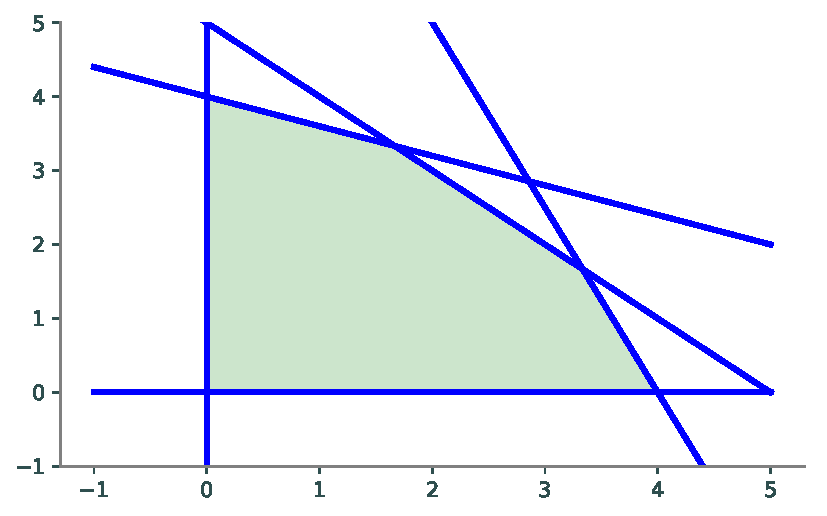
\includegraphics[width=\linewidth]{foundationsAppliedMathematicsLabs/Volume2/Simplex/figures/feasiblePolytope.pdf}
    \caption{The feasible region for a linear program with 2-dimensional constraints.}
\end{subfigure}%
\begin{subfigure}{.5\textwidth} % 3-d feasible polytope.
    \begin{center}
    \begin{tikzpicture}[dot/.style={circle,fill=blue,minimum size=3pt,inner sep=0pt, outer sep=-1pt}, >=stealth']

    \draw[blue!10!, fill=blue!5!](3,1)--(1.5,2.3)--(1.75,1.3)--cycle;
    \draw[blue!25!, fill = blue!15!](3,1)--(1.75,1.3)--(2.3,-1)--cycle;
    \draw[blue!55!, fill = blue!40!](1.75,1.3)--(2.3,-1)--(.8,-1)--cycle;
    \draw[blue!80!, fill = blue!65!](.8,-1)--(-.05,-.2)--(.25,.6)--(1.22,.06)--cycle;
    \draw[blue!85!, fill = blue!73!](-.05, -.2)--(-.3,0)--(.1, 1.65)--(.25, .6)--cycle;
    \draw[blue!65!, fill = blue!50!](.1,1.7)--(.25,.6)--(1.22,.07)--(1.75,1.3)--cycle;
    \draw[blue!40!, fill = blue!15!](.1,1.7)--(1.75,1.3)--(1.5,2.3)--cycle;

    \draw[-,thick](-.3,0)--(.1,1.7)--(1.5, 2.3)--(3, 1)--(2.3,-1)--(.8,-1)--cycle;

    \draw[-,thick](.1,1.7)--(3,1);
    \draw[-,thick](1.5, 2.3)--(2.3,-1);
    \draw[-,thick](.8,-1)--(1.74,1.3);
    \draw[-,thick](.1,1.7)--(.25,.6);
    \draw[-,thick](1.24,.07)--(.25,.6);
    \draw[-,thick](-.05,-.24)--(.25,.6);

    \draw[->](.37,.63)--(.22,1.61);
    \draw[->](.31,1.55)--(1.63,1.23);
    \draw[->](.75,-.85)--(1.12,.05);
    \draw[->](1.05,.05)--(.25,.48);
    \draw[->](1.83,1.35)--(1.65,2.1);

    \node[draw=none](x*)at(1.8,2.45){$\x^*$};

    \end{tikzpicture}
    \end{center}
    \caption{The feasible region for a linear program with 3-dimensional constraints.}
\end{subfigure}
\caption{If an optimal point exists, it is one of the vertices of the polyhedron.
The simplex algorithm searches for optimal points by moving between adjacent vertices in a direction that increases the value of the objective function until it finds an optimal vertex.}
\label{fig:polytope}
\end{figure}

% \begin{figure}[htb] % 3-d feasible polytope.
% \end{figure}


% % TODO: subfigure for 3-d polytope from book.

Implementing the Simplex Algorithm is straightforward, provided one carefully follows the procedure.
We will break the algorithm into several small steps, and write a function to perform each one.
To become familiar with the execution of the Simplex algorithm, it is helpful to work several examples by hand.

\subsection*{The Simplex Solver} % ===============================================

Our program will be more lengthy than many other lab exercises and will consist of a collection of functions working together to produce a final result.
It is important to clearly define the task of each function and how all the functions will work together.
If this program is written haphazardly, it will be much longer and more difficult to read than it needs to be.
We will walk you through the steps of implementing the Simplex Algorithm as a Python class.
% Since the Simplex Algorithm assumes that all the variables are non-negative, we do not need any special logic for it.
% what is this previous statement saying? What 'special logic' would you need if the variables were negative?

For demonstration purposes, we will use the following linear program.
\begin{align*}
\text{minimize}\qquad & -3x_0 - 2x_1 \\
\text{subject to}\qquad
& x_0 - x_1 \leq 2 \\
& 3x_0 + x_1 \leq 5 \\
& 4x_0 + 3x_1 \leq 7 \\
& x_0, x_1 \geq 0.
\end{align*}

\subsection*{Accepting a Linear Program} % ------------------------------------

Our first task is to determine if we can even use the Simplex algorithm.
Assuming that the problem is presented to us in standard form, we need to check that the feasible region includes the origin.  For now, we only check for feasibility at the origin. A more robust solver sets up the auxiliary problem and solves it to find a starting point if the origin is infeasible.

\begin{problem}{Check feasibility at the origin.}{}
Write a class that accepts the arrays $\c$, $A$, and $\b$ of a linear optimization problem in standard form.
In the constructor, check that the system is feasible at the origin.
That is, check that $A\x \preceq \b$ when $\x = \0$. Raise a \li{ValueError} if the problem is not feasible at the origin. \label{prob:initsolver}
\end{problem}

\subsection*{Adding Slack Variables} % ----------------------------------------

The next step is to convert the inequality constraints $A\x \leq \b$ into equality constraints by introducing a slack variable for each constraint equation.
If the constraint matrix $A$ is an $m \times n$ matrix, then there are $m$ slack variables, one for each row of $A$.
Grouping all of the slack variables into a vector $\w$ of length $m$, the constraints now take the form $A\x + \w = \b$.
In our example, we have \[\w = \left[\begin{array}{c}x_2\\x_3 \\x_4\end{array}\right]\]

% TODO: change the representation of the slack variables to match the book.
When adding slack variables, it is useful to represent all of your variables, both the original primal variables and the additional slack variables, in a convenient manner.
One effective way is to refer to a variable by its subscript.
For example, we can use the integers $0$ through $n-1$ to refer to the original (non-slack) variables $x_0$ through $x_{n-1}$, and we can use the integers $n$ through $n+m-1$ to track the slack variables (where the slack variable corresponding to the $i$th row of the constraint matrix is represented by the index $n+i-1$).

We also need some way to track which variables are \emph{independent} (non-zero) and which variables are \emph{dependent} (those that have value $0$). This can be done using the objective function. At anytime during the optimization process, the non-zero variables in the objective function are \emph{independent} and all other variables are \emph{dependent}. 

%A useful representation for the variables is a Python list (or NumPy array), where the elements of the list are integers.
%Since we know how many dependent variables we have ($m$), we can partition the list so that all the dependent variables are kept in the first $m$ locations, and all the independent variables are stored at the end of the list.
%The ordering of this list is important.
%In particular, if $i \leq m$, the $i$th element of the list represents the dependent variable corresponding to the $i$th row of $A$.
%Henceforth we will refer to this list as the \emph{index list}.

%Initially, the dependent variables are simply the slack variables, and their values correspond to the values of %the vector $\b$.
%In our example, we have 2 primal variables $x_0$ and $x_1$, and we must add 3 slack variables.
%Thus, we instantiate the following index list:

%\begin{lstlisting}
%>>> L = [2, 3, 4, 0, 1]
%\end{lstlisting}

%Notice how the first $3$ entries of the index list are $2, 3, 4$, the indices representing the slack variables.
%This reflects the fact that the dependent variables at this point are exactly the slack variables.

%As the Simplex Algorithm progresses, however, the dependent variables change, and it will be necessary to swap
%elements in our index list.
%For example, suppose the variable represented by the index $4$ becomes independent, while the variable %represented by index $0$ becomes dependent.
%In this case we swap these two entries in the index list.

%\begin{lstlisting}
%>>> L[2], L[3] = L[3], L[2]
%>>> L
%[2, 3, 0, 4, 1]
%\end{lstlisting}

%Now our index list tells us that the current dependent variables $2, 3, 0$.

%\begin{problem} % Slack variables. % TODO: this problem is worthless...
%Design and implement a way to store and track all of the dependent and independent variables.

%Hint: Using integers that represent the index of each variable is useful for Problem \ref{prob:blands}.
%\label{prob:slackvars}
%\end{problem}

\subsection*{Creating a Dictionary} % --------------------------------------------

After we have determined that our program is feasible, we need to create the \emph{dictionary} (sometimes called the \emph{tableau}), a matrix to track the state of the algorithm.
%Remember that your dictionary will need to include in some way the slack variables that you created in Problem \ref{prob:slackvars}.

There are many different ways to build your dictionary.
One way is to mimic the dictionary that is often used when performing the Simplex Algorithm by hand. To do this we will set the corresponding dependent variable equations to 0. For example, if $x_5$ were a dependent variable we would expect to see a -1 in the column that represents $x_5$.
Define \[\bar{A} = \left[\begin{array}{cc} A & I_m \end{array}\right],\]
where $I_m$ is the $m \times m$ identity matrix we will use to represent our slack variables, and define
\[\bar{\c} = \left[\begin{array}{c}\c\\ \0\end{array}\right].\]
That is, $\bar{\c} \in \mathbb{R}^{n+m}$ such that the first $n$ entries are $\c$ and the final $m$ entries are zeros.
Then the initial dictionary has the form
\begin{equation}
D =
\left[\begin{array}{ccc}
0  & \bar{\c}\trp \\
\b &  -\bar{A} 
\end{array}\right]
\label{eqn:hand_tab}
\end{equation}

The columns of the dictionary correspond to each of the variables (both primal and slack), and the rows of the dictionary correspond to the dependent variables.
%Using the convention introduced above of representing the variables by indices in the index list, we have the following correspondence:
%\[
%\text{column } i \Leftrightarrow \text{index } i-2, \qquad i = 2, 3, \ldots, n+m+1,
%\]
%and
%\[
%\text{row } j \Leftrightarrow L_{j-1}, \qquad j = 2, 3, \ldots, m+1,
%\]
%where $L_{j-1}$ refers to the $(j-1)$th entry of the index list.

%For our example problem, the initial index list is
%\[
%L = (2, 3, 4, 0, 1),
%\]
For our example the initial dictionary is
\begin{equation*}
D = \begin{bmatrix}
    0 & -3 & -2 & 0 & 0 & 0\\
    2 & -1 & 1 & -1 & 0 & 0\\
    5 & -3 & -1 & 0 & -1 & 0\\
    7 & -4 & -3 & 0 & 0 & -1
    \end{bmatrix}.
\end{equation*}
%The third column corresponds to index $1$, and the fourth row corresponds to index $4$, since this is the
%third entry of the index list.

The advantage of using this kind of dictionary is that it is easy to check the progress of your algorithm by hand.
%The disadvantage is that pivot operations require careful bookkeeping to track the variables and constraints.

% This dictionary is less intuitive, and I think could lead to more confusion.
\begin{comment}
We can also use a dictionary of the format:
\begin{equation}
T = \begin{bmatrix}
    0 & \c\trp  & 0 \\
    \0 & I_n & \0\\
    \b & -A  & \0
\end{bmatrix}.
\label{eqn:matrix_tab}
\end{equation}
Here, $T$ is a square matrix of size $(n+m+1) \times (n+m+1)$.
The advantage of this form of the dictionary is that all the pivot bookkeeping is built into the matrix.
For our example problem, the initial dictionary of this form is
\begin{equation}
T = \begin{bmatrix}
        0 & 3 & 2 & 0 & 0 & 0 \\
        0 & 1 & 0 & 0 & 0 & 0 \\
        0 & 0 & 1 & 0 & 0 & 0 \\
        2 &-1 & 1 & 0 & 0 & 0 \\
        5 &-3 &-1 & 0 & 0 & 0 \\
        7 &-4 &-3 & 0 & 0 & 0
\end{bmatrix}.
\label{eqn:matrix_inittab}
\end{equation}
\end{comment}

\begin{problem}{Initialize the dictionary.}
Add a method to your Simplex solver that takes in arrays c, A, and b to create the initial dictionary (D) as a NumPy array.
\label{prob:makedictionary}
\end{problem}

\subsection{Pivoting} % ------------------------------------------------------

Pivoting is the mechanism that really makes Simplex useful.
Pivoting refers to the act of swapping dependent and independent variables, and transforming the dictionary appropriately.
This has the effect of moving from one vertex of the feasible polytope to another vertex in a way that increases the value of the objective function.
Depending on how you store your variables, you may need to modify a few different parts of your solver to reflect this swapping.

When initiating a pivot, you need to determine which variables will be swapped.
In the dictionary representation, you first find a specific element on which to pivot, and the row and column that contain the pivot element correspond to the variables that need to be swapped.
Row operations are then performed on the dictionary so that the pivot column becomes a negative elementary vector.

Let's break it down, starting with the pivot selection.
We need to use some care when choosing the pivot element.
To find the pivot column, search from left to right along the top row of the dictionary (ignoring the first column), and stop once you encounter the first negative value.
The index corresponding to this column will be designated the \emph{entering index}, since after the full pivot operation, it will enter
the basis and become a dependent variable.

Using our initial dictionary $D$ in the example, we stop at the second column:
\[ D = \left[ \:
\begin{array}{*{7}{c}}
\cline{2-2}
0 & \multicolumn{1}{|c}{-3} & \multicolumn{1}{|c}{-2} & 0 & 0 & 0\\
2 & \multicolumn{1}{|c}{-1} & \multicolumn{1}{|c}{1} & -1 & 0 & 0\\
5 & \multicolumn{1}{|c}{-3} & \multicolumn{1}{|c}{-1} & 0 & -1 & 0\\
7 & \multicolumn{1}{|c}{-4} & \multicolumn{1}{|c}{-3} & 0 & 0 & -1\\
\cline{2-2}
\end{array}
\right] \]
We now know that our pivot element will be found in the second column.
The entering index is thus $1$.

Next, we select the pivot element from among the negative entries in the pivot column (ignoring the entry in the first row).
\emph{If all entries in the pivot column are non-negative, the problem is unbounded and has no solution.}
In this case, the algorithm should terminate.
Otherwise, assuming our pivot column is the $j$th column of the dictionary and that the negative entries of this column are
$D_{i_1, j}, D_{i_2, j}, \ldots, D_{i_k, j}$, we calculate the ratios
\[
\frac{-D_{i_1,0}}{D_{i_1,j}}, \frac{-D_{i_2,0}}{D_{i_2,j}}, \ldots, \frac{-D_{i_k,0}}{D_{i_k,j}},
\]
and we choose our pivot element to be one that minimizes this ratio.
If multiple entries minimize the ratio, then we utilize \emph{Bland's Rule}, which instructs us to choose the entry in the row corresponding to the smallest index (obeying this rule is important, as it prevents the possibility of the algorithm cycling back on itself infinitely).
The index corresponding to the pivot row is designated as the \emph{leaving index}, since after the full pivot operation, it will leave the basis and become a independent variable.

In our example, we see that all entries in the pivot column (ignoring the entry in the first row, of course) are negative, and hence they are all potential choices for the pivot element.
We then calculate the ratios, and obtain
\[
\frac{-2}{-1} = 2,\quad \frac{-5}{-3} = 1.66...,\quad \frac{-7}{-4} = 1.75.
\]
We see that the entry in the third row minimizes these ratios.
Hence, the element in the second column (index 1), third row (index 2) is our designated
pivot element.

\[ D = \left[ \:
\begin{array}{*{7}{c}}

0 & -3 & -2 & 0 & 0 & 0\\
2 & -1 & 1 & -1 & 0 & 0\\\cline{2-2}
5 & \multicolumn{1}{|c}{-3} & \multicolumn{1}{|c}{-1} & 0 & -1 & 0\\\cline{2-2}
7 & -4 & -3 & 0 & 0 & -1\\
\end{array}
\right] \]

\begin{comment}
If we are using the dictionary representation in equation \ref{eqn:matrix_tab}, pivot operations are reduced to a simple matrix equation:
\[T = T + T_m \otimes T_n,\]
where $T_m$ is the column corresponding to the variable entering the basis and $T_n$ is a normalized vector corresponding to the variable leaving the basis.
The result of the equation is the new dictionary.

For example, for the initial dictionary, \ref{eqn:matrix_inittab}, we will demonstrate the first pivot operation.
We can do the entire pivot with a single outer product.
The first pivot should occur with $x_1$ leaving and $x_4$ entering.
In other words, we want to pivot at row $i = 4$ and column $j = 1$ in the dictionary (the indices are offset by one because of the objective function and the row of constraints).

The row corresponding to $x_4$ is
\[
\begin{bmatrix} 5 &-3 &-1 & 0 & 0 & 0\end{bmatrix}.
\]
This represents the equation
\[
x_4 = 5 - 3x_1 - x_2.
\]
Our eventual goal is to solve for $x_1$ and substitute into the remaining rows of the dictionary.
A simple method to accomplish this is to rewrite the equation so that we have zero on the left-hand side:
\[
0 = 5 - 3x_1 - x_2 - x_4.
\]
Now, we can normalize this equation so that the coefficient of $x_1$ is $-1$.
This is always accomplished by dividing the equation by the negative of the coefficient of $x_1$:
\begin{equation}
0 = \frac{5}{3} - x_1 - \frac{1}{3}x_2 - \frac{1}{3}x_4.
\label{eq:zero-equation}
\end{equation}
This is represented by the vector
\[
\begin{bmatrix} 5/3 & -1 & -1/3 & 0 & -1/3 & 0\end{bmatrix}.
\]
Since this left-hand side is zero, I can add any scalar multiple of this equation to any of the equations for $x_i$ and still have an equation for $x_i$.
For example, the equation for $x_5$ is
\[
x_5 = 7 - 4x_1 - 3x_2.
\]
Thus, I can add $-4$ times \eqref{eq:zero-equation} to this equation without changing the left-hand side:
\[ x_5 = 7 - 4x_1 - 3x_2 = 7 - 4x_1 - 3x_2 + -4\left(\frac{5}{3} - x_1 - \frac{1}{3}x_2 - \frac{1}{3}x_4\right) = \frac{1}{3} - \frac{5}{3}x_2 + \frac{4}{3} x_4.
\]
Notice that we end up with an equation that does not include $x_1$ and now has $x_4$, just like we wanted.
In fact, this works in all of our equations, including those for the objective function and even for $x_1$!
Since the coefficient of $x_1$ in \eqref{eq:zero-equation} is $-1$, when we scale it by the coefficient of $x_1$ in any particular row, the $x_1$ cancels out.
\[
T = T + \begin{bmatrix}3 \\ 1 \\ 0 \\ -1 \\ -3 \\ -4\end{bmatrix}\begin{bmatrix} 5/3 & -1 & -1/3 & 0 & -1/3 & 0\end{bmatrix}.
\]
The column vector is just the second column of $T$, which is the column containing the coefficients of $x_1$ in each row.
When we compute this sum, we obtain the dictionary.
\[
T = \begin{bmatrix}
        5 &  0 & 1 & 0 & -1 & 0 \\
        5/3 & 0 &-1/3 & 0 &-1/3 & 0 \\
        0 & 0 & 1 & 0 & 0 & 0 \\
        1/3 & 0 & 4/3 & 0 & 1/3 & 0 \\
        0 & 0 & 0 & 0 & 1 & 0 \\
        1/3 & 0 & -5/3 & 0 & 4/3 & 0
\end{bmatrix}.
\]
\end{comment}
%\begin{problem}
%Write a method that will determine the pivot row and pivot column according to Bland's Rule.
% \begin{comment}
\begin{definition}{Bland's Rule}
Choose the independent variable with the smallest index that has a negative coefficient in the objective function
as the leaving variable.
Choose the dependent variable with the smallest index among all the binding dependent variables.
\end{definition}

Bland's Rule is important in avoiding cycles when performing pivots.
This rule guarantees that a feasible Simplex problem will terminate in a finite number of pivots.% \emph{Hint:} Avoid dividing by zero.
% \end{comment}
%\label{prob:blands}
%\end{problem}

%The next step is to swap the entering and leaving indices in our index list.
%In the example, we determined above that these indices are $0$ and $3$.
%We swap these two elements in our index list,
%and the updated index list is now
%\[
%L = (2, 0, 4, 3, 1),
%\]
%so the dependent variables are now given by the indices $2, 0, 4$.

Finally, we perform row operations on our dictionary in the following way: divide the pivot row by the negative value of the pivot entry.
Then use the pivot row to zero out all entries in the pivot column above and below the pivot entry.
In our example, we first divide the pivot row by -3, and then zero out the two entries above the pivot element and the single entry below it:
\begin{align*}
\begin{bmatrix}
    0 & -3 & -2 & 0 & 0 & 0\\
    2 & -1 & 1 & -1 & 0 & 0\\
    5 & -3 & -1 & 0 & -1 & 0\\
    7 & -4 & -3 & 0 & 0 & -1
    \end{bmatrix} &\rightarrow
\begin{bmatrix}
    0 & -3 & -2 & 0 & 0 & 0\\
    2 & -1 & 1 & -1 & 0 & 0\\
    5/3 & -1 & -1/3 & 0 & -1/3 & 0\\
    7 & -4 & -3 & 0 & 0 & -1
    \end{bmatrix}\rightarrow\\
\begin{bmatrix}
    -5 & 0 & -1 & 0 & 1 & 0\\
    2 & -1 & 1 & -1 & 0 & 0\\
    5/3 & -1 & -1/3 & 0 & -1/3 & 0\\
    7 & -4 & -3 & 0 & 0 & -1
    \end{bmatrix} &\rightarrow
\begin{bmatrix}
    -5 & 0 & -1 & 0 & 1 & 0\\
    1/3 & 0 & -4/3 & 1 & -1/3 & 0\\
    5/3 & -1 & -1/3 & 0 & -1/3 & 0\\
    7 & -4 & -3 & 0 & 0 & -1
    \end{bmatrix}\rightarrow\\
\begin{bmatrix}
    -5 & 0 & -1 & 0 & 1 & 0\\
    1/3 & 0 & 4/3 & -1 & 1/3 & 0\\
    5/3 & -1 & -1/3 & 0 & -1/3 & 0\\
    1/3 & 0 & -5/3 & 0 & 4/3 & -1
    \end{bmatrix}&.
\end{align*}
The result of these row operations is our updated dictionary, and the pivot operation is complete.

\begin{problem}{Pivoting}
Add a method to your solver that checks for unboundedness and performs a single pivot operation from start to completion.
If the problem is unbounded, raise a \li{ValueError}.
\end{problem}

\vspace{2mm}

\subsection{Termination and Reading the Dictionary} % ---------------------------

Up to this point, our algorithm accepts a linear program, adds slack variables, and creates the initial dictionary.
After carrying out these initial steps, it then performs the pivoting operation iteratively until the optimal point is found.
But how do we determine when the optimal point is found? The answer is to look at the top row of the dictionary, which represents the objective function.
More specifically, before each pivoting operation, check whether all of the entries in the top row of the dictionary (ignoring the entry in the first column) are nonnegative.
If this is the case, then we have found an optimal solution, and so we terminate the algorithm.

The final step is to report the solution.
The ending state of the dictionary and index list tells us everything we need to know.
The minimal value attained by the objective function is found in the upper leftmost entry of the dictionary.
The dependent variables all have the value $0$ in the objective function or first row of our dictionary array. The independent variables have values given by the first column of the dictionary.
Specifically, the independent variable whose index is located at the $i$th entry of the index list has the value $T_{i+1, 0}$.

In our example, suppose that our algorithm terminates with the dictionary and index list in the following state:
\[
D = \begin{bmatrix}
-5.2 & 0 & 0 & 0 & 0.2 & 0.6\\
0.6 & 0 & 0 & -1 & 1.4 & -0.8\\
1.6 & -1 & 0 & 0 & -0.6 & 0.2\\
0.2 & 0 & -1 & 0 & 0.8 & -0.6\\
\end{bmatrix}
\]
%\[
%L = (2, 0, 1, 3, 4).
%\]
Then the minimal value of the objective function is $-5.2$.
The independent variables have indices $4, 5$ and have the value $0$.
The dependent variables have indices $3, 1,$ and $2$, and have values $.6, 1.6$, and $.2$, respectively.
In the notation of the original problem statement, the solution is given by
\begin{align*}
x_0 &= 1.6\\
x_1 &= .2.
\end{align*}

\begin{problem}{SimplexSolver.solve()}
Write an additional method in your solver called \li{solve()} that obtains the optimal solution, then returns the minimal value, the dependent variables, and the independent variables.
The dependent and independent variables should be represented as two dictionaries that map the index of the variable to its corresponding value.

For our example, we would return the tuple 

\li{(-5.2, \{0: 1.6, 1: .2, 2: .6\}, \{3: 0, 4: 0\})}.
%The correct format of this tuple is critical, as this tuple of information will be used judge whether or not your solver works!
\end{problem}

\vspace{5mm}

At this point, you should have a Simplex solver that is ready to use.
The following code demonstrates how your solver is expected to behave:

\vspace{5mm}

\begin{lstlisting}
>>> import SimplexSolver

# Initialize objective function and constraints.
>>> c = np.array([-3., -2.])
>>> b = np.array([2., 5, 7])
>>> A = np.array([[1., -1], [3, 1], [4, 3]])

# Instantiate the simplex solver, then solve the problem.
>>> solver = SimplexSolver(c, A, b)
>>> sol = solver.solve()
>>> print(sol)
(-5.2,
 {0: 1.6, 1: 0.2, 2: 0.6},
 {3: 0, 4: 0})
\end{lstlisting}

If the linear program were infeasible at the origin or unbounded, we would expect the solver to alert the user by raising an error.

Note that this simplex solver is \emph{not} fully operational.
It can't handle the case of infeasibility at the origin.
This can be fixed by adding methods to your class that solve the \emph{auxiliary problem}, that of finding an initial feasible dictionary when the problem is not feasible at the origin.
Solving the auxiliary problem involves pivoting operations identical to those you have already implemented, so adding this functionality
is not overly difficult.


\subsection{Exercises}

\paragraph{Exercise $1.0$ (Learn $\mathrm{LT}_{\mathrm{E}} \mathrm{X}$ )}

Learn to use $\operatorname{lt}_{\mathrm{E}} X$ for writing all of your homework solutions. Personally, I use MiKTEX, which is an implementation of $\mathrm{ET} \mathrm{E} \mathrm{X}$ for Windows. Specifically, within MiKTEX I am using pdfteTEX (it only matters for certain things like including graphics and also pdf into a document). I find it convenient to use the editor WinEdt, which is very LATEX friendly. A good book on $\mathrm{ET} \mathrm{T} \mathrm{X}$ is

In A.1 there is a template to get started. Also, there are plenty of tutorials and beginner's guides on the web.

\paragraph{Exercise $1.1$ (Convert to standard form)}

Give an original example (i.e., with actual numbers) to demonstrate that you know how to transform a general linear-optimization problem to one in standard form.

\paragraph{Exercise $1.2$ (Weak Duality example)}

Give an original example to demonstrate the Weak Duality Theorem.

\paragraph{Exercise $1.3$ (Convert to $\leq$ form)}

Describe a general recipe for transforming an arbitrary linear-optimization problem into one in which all of the linear constraints are of $\leq$ type.

\paragraph{Exercise $1.4$ ( $m+1$ inequalities)}

Prove that the system of $m$ equations in $n$ variables $A x=b$ is equivalent to the system $A x \leq b$ augmented by only one additional linear inequality - that is, a total of only $m+1$ inequalities.

\paragraph{Exercise $1.5$ (Weak duality for another form)}

Give and prove a Weak Duality Theorem for

$$
\begin{aligned}
\max \quad c^{\prime} x & \\
A x & \leq b ; \\
x & \geq 0 .
\end{aligned}
$$

HINT: Convert $\left(\mathrm{P}^{\prime}\right)$ to a standard-form problem, and then apply the ordinary Weak Duality Theorem for standard-form problems. \paragraph{Exercise 1.6 (Weak duality for a complicated form)}

Give and prove a Weak Duality Theorem for

$$
\begin{gathered}
\min \quad c^{\prime} x+f^{\prime} w \\
\begin{aligned}
A x+B w & \leq b ; \\
D x &=g ;
\end{aligned} \\
x \geq 0 \quad w \leq 0
\end{gathered}
$$

HINT: Convert $\left(\mathrm{P}^{\prime}\right)$ to a standard-form problem, and then apply the ordinary Weak Duality Theorem for standard-form problems.

\paragraph{Exercise $1.7$ (Weak duality for a complicated form - with MATLAB)}

The MATLAB code below makes and solves an instance of $\left(\mathrm{P}^{\prime}\right)$ from Exercise 1.6. Study the code to see how it is works. Now, extend the code to solve the dual of $\left(\mathrm{P}^{\prime}\right)$. Also, after converting $\left(\mathrm{P}^{\prime}\right)$ to standard form (as indicated in the HINT for Exercise 1.6), use MATLAB to solve that problem and its dual. Make sure that you get the same optimal value for all of these problems.





\subsection{$2.5$ Exercises}

\paragraph{Exercise 2.1 (Dual in AMPL)}

Without changing the file production. dat, use AMPL to solve the dual of the Production Problem example, as described in Section 2.1. You will need to modify production.mod and production.run.

\paragraph{Exercise $2.2$ (Sparse solution for linear equations with AMPL)}

In some application areas, it is interesting to find a "sparse solution" - that is, one with few non-zeros - to a system of equations $A x=b$. It is well known that a 1-norm minimizing solution is a good heuristic for finding a sparse solution. Using AMPL, try this idea out on several large examples, and report on your results.

HINT: To get an interesting example, try generating a random $m \times n$ matrix $A$ of zeros and ones, perhaps $m=50$ equations and $n=500$ variables, maybe with probability $1 / 2$ of an entry being equal to one. Then choose maybe $m / 2$ columns from $A$ and add them up to get $b$. In this way, you will know that there is a solution with only $m / 2$ non-zeros (which is already pretty sparse). Your 1-norm minimizing solution might in fact recover this solution $(\odot)$, or it may be sparser $(\odot \odot)$, or perhaps less sparse $(\odot)$.

\paragraph{Exercise $2.3$ (Bloody AMPL)}

A transportation problem is a special kind of (single-commodity min-cost) networkflow problem. There are certain nodes $v$ called supply nodes which have net supply $b_{v}>0$. The other nodes $v$ are called demand nodes, and they have net supply $b_{v}<0$. There are no nodes with $b_{v}=0$, and all arcs point from supply nodes to demand nodes.

A simplified example is for matching available supply and demand of blood, in types $A, B, A B$ and $O$. Suppose that we have $s_{v}$ units of blood available, in types $v \in\{A, B, A B, O\}$. Also, we have requirements $d_{v}$ by patients of different types $v \in$ $\{A, B, A B, O\}$. It is very important to understand that a patient of a certain type can accept blood not just from their own type. Do some research to find out the compatible blood types for a patient; don't make a mistake - lives depend on this! In this spirit, if your model misallocates any blood in an incompatible fashion, you will receive a grade of $F$ on this problem.

Describe a linear-optimization problem that satisfies all of the patient demand with compatible blood. You will find that type $O$ is the most versatile blood, then both $A$ and $B$, followed by $A B$. Factor in this point when you formulate your objective function, with the idea of having the left-over supply of blood being as versatile as possible.

Using AMPL, set up and solve an example of a blood-distribution problem.

\paragraph{Exercise $2.4$ (Mix it up)}

"I might sing a gospel song in Arabic or do something in Hebrew. I want to mix it up and do it differently than one might imagine." - Stevie Wonder

We are given a set of ingredients $1,2, \ldots, m$ with availabilities $b_{i}$ and per unit costs $c_{i}$. We are given a set of products $j, 2, \ldots, m$ with minimum production requirements $d_{j}$ and per unit revenues $e_{j}$. It is required that product $j$ have at least a fraction of $l_{i j}$ of ingredient $i$ and at most a fraction of $u_{i j}$ of ingredient $i$. The goal is to devise a plan to maximize net profit.

Formulate, mathematically, as a linear-optimization problem. Then, model with AMPL, make up some data, try some computations, and report on your results. Exercise $2.5$ (Task scheduling)


We are given a set of tasks, numbered $1,2, \ldots, n$ that should be completed in the minimum amount of time. For convenience, task 0 is a "start task" and task $n+1$ is an "end task". Each task, except for the start and end task, has a known duration $d_{i}$. For convenience, let $d_{0}:=0$. There are precedences between tasks. Specifically, $\Psi_{i}$ is the set of tasks that must be completed before task $i$ can be started. Let $t_{0}:=0$, and for all other tasks $i$, let $t_{i}$ be a decision variable representing its start time.

Formulate the problem, mathematically, as a linear-optimization problem. The objective should be to minimize the start time $t_{n+1}$ of the end task. Then, model the problem with AMPL, make up some data, try some computations, and report on your results.

\paragraph{Exercise $2.6$ (Investing wisely)}

Almost certainly, Albert Einstein did not say that "compound interest is the most powerful force in the universe."

A company wants to maximize their cash holdings after $T$ time periods. They have an external inflow of $p_{t}$ dollars at the start of time period $t$, for $t=1,2, \ldots, T$. At the start of each time period, available cash can be allocated to any of $K$ different investment vehicles (in any available non-negative amounts). Money allocated to investmentvehicle $k$ at the start of period $t$ must be held in that investment $k$ for all remaining time periods, and it generates income $v_{t, t}^{k}, v_{t, t+1}^{k}, \ldots, v_{t T}^{k}$, per dollar invested. It should be assumed that money obtained from cashing out the investment at the end of the planning horizon (that is, at the end of period $T$ ) is part of $v_{t, T}^{k}$. Note that at the start of time period $t$, the cash available is the external inflow of $p_{t}$, plus cash accumulated from all investment vehicles in prior periods that was not reinvested. Finally, assume that cash held over for one time period earns interest of $q$ percent.

Formulate the problem, mathematically, as a linear-optimization problem. Then, model the problem with AMPL, make up some data, try some computations, and report on your results.



\section{Finding Feasible Basis}

\underline{\bf Finding an Initial BFS}
When a basic feasible solution is not apparent, we an produce one using {\it artificial variables}.  This {\it artificial} basis is undesirable from the perspective of the original problem, we do not want the artificial variables in our solution, so we penalize them in the objective function, and allow the simplex algorithm to drive them to zero (if possible) and out of the basis.  There are two such methods, the {\bf Big M method} and the {\bf Two-phase method}, which we illustrate below:

\vspace{10mm}  Solve the following LP using the Big M Method and the simplex algorithm:

\begin{align*}
max~~ & z = 9x_1 + 6x_2 \\
s.t.~~
&  3x_1 + 3x_2 \le 9 \\
&  2x_1 - 2x_2 \ge 3 \\
&  2x_1 + 2x_2 \ge 4 \\
& x_1, x_2 \ge 0. \\
\end{align*}

Here is the LP is transformed into standard form by using slack variables $x_3$, $x_4$, and $x_5$, with the required artificial variables $x_6$ and $x_7$, which allow us to easily find an initial basic feasible solution (to the artificial problem).
\begin{eqnarray}
& max  & z_a = 9x_1 + 6x_2 -M x_6 - M x_7 \nonumber \\
& s.t. & 3x_1 + 3x_2 + x_3 = 9 \nonumber \\
&      & 2x_1 - 2x_2 - x_4 + x_6 = 3 \nonumber \\
&      & 2x_1 + 2x_2 - x_5 + x_7 = 4 \nonumber \\
&      & x_i \ge 0,~~ i =1,\cdots,7. \nonumber
\end{eqnarray}

\begin{center} \begin{tabular} {|c|c|c|c|c|c|c|c||c| r} \cline{1-9}
$z$	& $x_1$	& $x_2$	& $x_3$	& $x_4$	& $x_5$	& $x_6$	& $x_7$	& RHS &	ratio \\ \cline{1-9}
1	&	 -9 &	 -6 &	 0 &	  0 &	  0 &	  M &	  M &	0 & \\
0	&	  3 &	  3 &	 1 &	  0 &	  0 &	  0 &	  0 &	9 &	 \\
0	&	  2 &	 -2 &	 0 &	 -1 &	  0 &	  1 &	  0 &	3 & \\
0	&	  2 &	  2 &	 0 &	  0 &	 -1 &	  0 &	  1 &	4 &	 \\
\cline{1-9}
\end{tabular} \end{center}
\noindent This tableau is not in the correct form, it does not represent a basis, the columns for the artificial variables need to be adjusted.

\begin{center} \begin{tabular} {|c|c|c|c|c|c|c|c||c| r} \cline{1-9}
$z$	& $x_1$	  & $x_2$  & $x_3$	& $x_4$	& $x_5$	& $x_6$	& $x_7$	& RHS &	ratio \\ \cline{1-9}
1	& -9 - 4M & -6     &	 0 &	  M &	  M &	  0 &	  0 & -7M &	      \\
0	&	  3   &	     3 &	 1 &	  0 &	  0 &	  0 &	  0 &	9 &	3     \\
0	&	  2   &	    -2 &	 0 &	 -1 &	  0 &	  1 &	  0 &	3 &	3/2   \\
0	&	  2   &	     2 &	 0 &	  0 &	 -1 &	  0 &	  1 &	4 &	2     \\
\cline{1-9}
\end{tabular} \end{center}
\noindent The current solution is not optimal, so $x_1$ enters the basis, and by the ratio test, $x_6$ (an artificial variable) leaves the basis.

\begin{center} \begin{tabular} {|c|c|c|c|c|c|c|c||c| r} \cline{1-9}
$z$	&   $x_1$ & $x_2$   & $x_3$	& $x_4$	& $x_5$	& $x_6$	   & $x_7$	& RHS      & ratio \\
\cline{1-9}
1	&     0   & -15 -4M &	 0 & -9/2 -M &	  M & 9/2 + 2M &	  0 &  27/2 -M &    	\\
0	&	  0   &	     6  &	 1 &	 3/2 &	  0 &	    -3/2 &	  0 &	3/2    & 3/4     \\
0	&	  1   &	    -1  &	 0 &	-1/2 &	  0 &	   1/2 &	  0 &	3/2    & -  	\\
0	&	  0   &	     4  &	 0 &	   1 &	 -1 &	     -1 &	  1 &	  1    & 1/4        	\\ \cline{1-9}
\end{tabular} \end{center}
\noindent The current solution is not optimal, so $x_2$ enters the basis, and by the ratio test, $x_7$ (an artificial variable) leaves the basis.

\begin{center} \begin{tabular} {|c|c|c|c|c|c|c|c||c|r} \cline{1-9}
$z$	&   $x_1$ & $x_2$ & $x_3$ & $x_4$	& $x_5$	& $x_6$	   & $x_7$	& RHS     &	ratio \\
\cline{1-9}
1	&     0   &     0 &	 0    & -3/4    & -15/4 &        - &	  - &  17 1/4 &	   \\
0	&	  0   &	    0 &	 1    &	   0    &	3/2 &	     0 &   -3/2 &	  3   &	-  \\
0	&	  1   &	    0 &	 0    &	-1/4    &  -1/4 &	   1/2 &	1/4 &	  7/4 &	-  	\\
0	&	  0   &	    1 &	 0    &	 1/4    &  -1/4 &	  -1/4 &	1/4 &	  1/4 & 1   \\
\cline{1-9}
\end{tabular} \end{center}
\noindent The current solution is not optimal, so $x_4$ enters the basis, and by the ratio test, $x_2$ leaves the basis.

\begin{center} \begin{tabular} {|c|c|c|c|c|c|c|c||c|r} \cline{1-9}
$z$	&   $x_1$ & $x_2$ & $x_3$ & $x_4$ & $x_5$ & $x_6$ & $x_7$ & RHS     &	ratio \\
\cline{1-9}
1	&     0   &    3  &	 0    & 0     & -9/2  &     - &	    - &  18 &	   \\
0	&	  0   &	    0 &	 1    &	   0  &	  3/2 &	    0 &  -3/2 &	  3     &	-  \\
0	&	  1   &	    1 &	 0    &	0     &  -1/2 &	   0  &	  1/2 &	  2   &	-  	\\
0	&	  0   &	    4 &	 0    &	 1    &  -1   &	  -1 &      1 &	  1    & 1   \\ \cline{1-9}
\end{tabular} \end{center}
\noindent The current solution is not optimal, so $x_5$ enters the basis, and by the ratio test, $x_3$ leaves the basis.

\begin{center} \begin{tabular} {|c|c|c|c|c|c|c|c||c|r} \cline{1-9}
$z$	&   $x_1$ & $x_2$ & $x_3$ & $x_4$ & $x_5$ & $x_6$ & $x_7$ & RHS     &	ratio \\
\cline{1-9}
1	&     0   &    3  &	 3    & 0     & 0  &     - &	    - &  27 &	   \\
0	&	  0   &	    0 &	 2/3  &	  0   &	  1 &	    0 &  -1 &	  2     &	 \\
0	&	  1   &	    1 &	 1/3   &   0  &  0 &	   0  &	  0 &	  3   &  	\\
0	&	  0   &	    4 &	 2/3   &	1 &  0   &	  -1 &     0&	 3    &    \\
\cline{1-9}
\end{tabular} \end{center}
The current solution is optimal! \\

\bigskip Solve the following LP using the Two-phase Method and Simplex Algorithm.
\begin{align*}
max~~ & z = 2x_1 + 3x_2   \\
s.t.~~ 
& 3x_1 + 3x_2 \ge 6  \\
& 2x_1 - 2x_2 \le 2  \\
& -3x_1 + 3x_2 \le 6   \\
& x_1, x_2 \ge 0. 
\end{align*}


%\begin{center} \includegraphics[scale=0.7]{Figs_N/TwoPhase}\end{center}

Here is first phase LP (in standard form), where $x_3$, $x_4$, and $x_5$ are slack variables, and $x_6$ is an artificial variable.
\begin{eqnarray}
& min  & z_a = x_6 \nonumber \\
& s.t. & 3x_1 + 3x_2 - x_3 +x_6 = 6 \nonumber \\
&      & 2x_1 - 2x_2 + x_4 = 2 \nonumber \\
&      & -3x_1 + 3x_2 + x_5 = 6 \nonumber \\
&      & x_i \ge 0,~~ i =1,\cdots,6. \nonumber
\end{eqnarray}
Next, we put the LP into a tableau, which, still is not in the right form for our basic variables ($x_6$, $x_4$, and $x_5$).
\begin{center} \begin{tabular} {|c|c|c|c|c|c|c||c| r} \cline{1-8}
$z$	& $x_1$	& $x_2$	& $x_3$	& $x_4$	& $x_5$	& $x_6$	&  RHS & ratio \\ \cline{1-8}
1	&	  0 &	  0 &	 0 &	  0 &	  0 &	 -1 &    0 & \\
0	&	  3 &	  3 &	-1 &	  0 &	  0 &	  1 &	 6 & \\
0	&	  2 &	 -2 &	 0 &	  1 &	  0 &	  0 &	 2 & \\
0	&	  -3 &	  3 &	 0 &	  0 &	  1 &	  0 &	 6 & \\ \cline{1-8}
\end{tabular} \end{center}
To remedy this, we use row operation to modify the row 0 coefficients, yielding the following:
\begin{center} \begin{tabular} {|c|c|c|c|c|c|c||c| r} \cline{1-8}
$z$	& $x_1$	& $x_2$	& $x_3$	& $x_4$	& $x_5$	& $x_6$	&  RHS & ratio \\ \cline{1-8}
1	&	  3 &	  3 &	 -1 &	  0 &	  0 &	  0 &    6 &   \\
0	&	  3 &	  3 &	-1 &	  0 &	  0 &	  1 &	 6 &  2 \\
0	&	  2 &	 -2 &	 0 &	  1 &	  0 &	  0 &	 2 &  - \\
0	&	  -3 &	  3 &	 0 &	  0 &	  1 &	  0 &	 6 &  2 \\ \cline{1-8}
\end{tabular} \end{center}
The current solution is not optimal, either $x_1$ or $x_2$ can enter the basis, let's choose $x_2$. Then by the ratio test, either $x_6$ (an artificial variable) or $x_5$ (a slack variable) can leaves the basis.  Let's choose $x_6$.
\begin{center} \begin{tabular} {|c|c|c|c|c|c|c||c| r} \cline{1-8}
$z$	& $x_1$	& $x_2$	& $x_3$	& $x_4$	& $x_5$	& $x_6$	&  RHS & ratio \\ \cline{1-8}
1	&	  0 &	  0 &	 0 &	  0 &	  0 &  -1 &    0 & \\
0	&	  1 &	  1 &	-1/3 &	  0 &	  0 &   1/3 &	 2 & \\
0	&	  4 &	  0 &	-2/3 &	  1 &	  0 &   2/3 &	 6 & \\
0	&	 -6 &	  0 &	 1 &	  0 &	  1 &	 -1 &	 0 & \\ \cline{1-8}
\end{tabular} \end{center}
The current solution is optimal, so we end the first phase with a basic feasible solution to the original problem, with $x_2$, $x_4$, and $x_5$ as the basic variables.  Now we provide a new row zero that corresponds to the original problem.

\begin{center} \begin{tabular} {|c|c|c|c|c|c|c||c| r} \cline{1-8}
$z$	& $x_1$	& $x_2$	& $x_3$	& $x_4$	& $x_5$	& $x_6$	&  RHS & ratio \\ \cline{1-8}
1	&	  1 &	  0 &	 -1 &	  0 &	  0 &	  0 &   6 & \\
0	&	  1 &	  1 &	-1/3 &	  0 &	  0 &	  1/3 &	 2 &   \\
0	&	  4 &	  0 &	-2/3 &	  1 &	  0 &	  2/3 &	 6 &  \\
0	&	 -6 &	  0 &	 1 &	  0 &	  1 &	  -1 &	 0 &  \\ \cline{1-8}
\end{tabular} \end{center}

\begin{center} \begin{tabular} {|c|c|c|c|c|c|c||c| r} \cline{1-8}
$z$	& $x_1$	& $x_2$	& $x_3$	& $x_4$	& $x_5$	& $x_6$	&  RHS & ratio \\ \cline{1-8}
1	&	 -5 &	  0 &	  0 &	  0 &	  1 &	  -1 &   6 & \\
0	&	 -1 &	  1 &	  0 &	  0 &	1/3 &	  0 &	 2 &   \\
0	&	  0 &	  0 &	  0 &	  1 &	2/3 &	  0 &	 6 &  \\
0	&	 -6 &	  0 &	  1 &	  0 &	  1 &	  -1 &	 0 &  \\ \cline{1-8}
\end{tabular} \end{center}
From this tableau we can see that the LP is unbounded and an extreme point is [0, 2, 0, 6,0] and an extreme direction is [1, 1, 6, 0, 0].




\underline{\bf Degeneracy and the Simplex Algorithm}
\begin{comment}
$\mathbf {n} \cdot (\mathbf {r} -\mathbf {r} _{0})=0.$
(The dot here means a dot (scalar) product.) Expanded this becomes

$a(x-x_{0})+b(y-y_{0})+c(z-z_{0})=0$
which is the point-normal form of the equation of a plane.  This is just a linear equation

$ax+by+cz+d=0$,
where

$d=-(ax_{0}+by_{0}+cz_{0}).$  
Conversely, it is easily shown that if a, b, c and d are constants and a, b, and c are not all zero, then the graph of the equation

$ax+by+cz+d=0$ is a plane having the vector 

$\mathbf{ n} = (a, b, c)$ as a normal. 

This plane can also be described by the "point and a normal vector" prescription above. A suitable normal vector is given by the cross product
${\mathbf {n}}=({\mathbf {p}}_{2}-{\mathbf {p}}_{1})\times ({\mathbf {p}}_{3}-{\mathbf {p}}_{1})$,

and the point r0 can be taken to be any of the given points p1,p2 or p3[6] (or any other point in the plane).
Let p1=(x1, y1, z1), p2=(x2, y2, z2), and p3=(x3, y3, z3) be non-collinear points.

${\displaystyle \mathbf {w\times v} ={\begin{vmatrix}\mathbf {i} &\mathbf {j} &\mathbf {k} \\w_{1}&w_{2}&w_{3}\\v_{1}&v_{2}&v_{3}\\\end{vmatrix}}}$

${\displaystyle {\begin{aligned}\mathbf {w\times v} &={\begin{vmatrix}w_{2}&w_{3}\\v_{2}&v_{3}\end{vmatrix}}\mathbf {i} -{\begin{vmatrix}w_{1}&w_{3}\\v_{1}&v_{3}\end{vmatrix}}\mathbf {j} +{\begin{vmatrix}w_{1}&w_{2}\\v_{1}&v_{2}\end{vmatrix}}\mathbf {k} \\&=(w_{2}v_{3}-w_{3}v_{2})\mathbf {i} +(w_{3}v_{1}-w_{1}v_{3})\mathbf {j} +(w_{1}v_{2}-w_{2}v_{1})\mathbf {k} ,\end{aligned}}}$
\end{comment}

Degeneracy must be considered in the simplex algorithm, as it causes some trouble.  For instance, it might mislead us into thinking there are multiple optimal solutions, or provide faulty insight.  Further, the algorithm as described can {\it cycle}, that is, remain on a degenerate extreme point repeatedly cycling through a subset of bases that represent that point, never leaving. 

\begin{center} \begin{tabular} {c|c|c|c|c|c|c|c|c|c|} \cline{2-10}
min &$z$	& $x_1$ & $x_2$ & $x_3$	& $x_4$	&  $x_5 $& $x_6$ & $x_7$ & $rhs$ \\ \cline{2-10}
       &1		& 0 		  & 0         &	 0 	    &	  3/4     &   -20 & 1/2 & -6  &     0    \\ \cline{2-10}
       &0		&	 1       &	    0   &	 0 			&	  1/4 		&	-8 & -1 &   9 &   0	  \\
       &0		&	 0     &	    1      &	 0 		&	  1 /2		&	 -12 & -1/2 & 3 & 0   \\ 
       &0		&	 0     &	    0      &	 1 		&	  0		&	 0 & 1 & 0 &1   \\ \cline{2-10}
\end{tabular} \end{center}


\bigskip  Solve the following LP using the Simplex Algorithm:
\begin{eqnarray}
& \max  & z = 40x_1 + 30x_2 \nonumber \\
& s.t. & 6x_1 + 4x_2 \le 40 \nonumber \\
&      & 4x_1 + 2x_2 \le 20 \nonumber \\
&      & x_1, x_2 \ge 0. \nonumber
\end{eqnarray}

By adding slack variables, we have the following tableau.
\begin{table}[h!] \begin{center} \begin{tabular} {|c|c|c|c|c||c|}
\hline
$z$ & $x_1$ & $x_2$ & $s_1$ & $s_2$ & RHS \\ \hline
  1 & -40 & -30 & 0   & 0   & 0  \\
  0 &   6 &   4 & 1   & 0   & 40 \\
  0 &   4 &   2 & 0   & 1   & 20 \\ \hline
\end{tabular} \end{center} \end{table}
Luckily, this tableau represents a basis, where BV=$\{s_1, s_2\}$, but by inspecting the row 0 (objective function row) coefficients, we can see that this is not optimal. By Dantzig's Rule, we enter $x_1$ into the basis, and by the ratio test we see that $s_2$ leaves the basis.  By performing elementary row operations, we obtain the following tableau for
the new basis BV=$\{s_1, x_1\}$.
\begin{center} \begin{tabular} {|c|c|c|c|c||c|} \hline
$z$ & $x_1$ & $x_2$ & $s_1$ & $s_2$ & RHS \\
\hline
  1 &     0 &   -10 & 0     &    10 & 200 \\
  0 &     0 &     1 & 1     &  -3/2 & 10 \\
  0 &     1 &   1/2 & 0     &   1/4 &  5 \\
\hline
\end{tabular} \end{center}

This tableau is not optimal, entering $x_2$ into the basis can improve the objective function value. The basic variables $s_1$ and $x_1$ tie in the ration test.  If we have $x_1$ leave the basis, we get the following tableau (BV=$\{s_1, x_2\}$).
\begin{center} \begin{tabular} {|c|c|c|c|c||c|}
\hline
$z$ & $x_1$ & $x_2$ & $s_1$ & $s_2$ & RHS \\
\hline
  1 &    20 &     0 &     0 &    15 & 300 \\
  0 &    -2 &     0 &     1 &    -2 &  0 \\
  0 &     2 &     1 &     0 &   1/2 &  10 \\ \hline
\end{tabular} \end{center}
This is an optimal tableau, with an objective function value of 300,  If instead of $x_1$ leaving the basis, suppose $s_1$ left, this would lead to the following tableau (BV=$\{x_2, x_1\}$).
\begin{center} \begin{tabular} {|c|c|c|c|c||c|} \hline
$z$ & $x_1$ & $x_2$ & $s_1$ & $s_2$ & RHS \\
\hline
  1 &     0 &     0 &    10 &    -5 & 300 \\
  0 &     0 &     1 &     1 &  -3/2 &  10 \\
  0 &     1 &     0 &  -1/2 &     1 &   0 \\ \hline
\end{tabular} \end{center}
This tableau does not look optimal, yet the objective function value is the same as the optimal solution's. This occurs because the optimal extreme point is a degenerate.% as the following figure shows.






% Copyright 2022 by Robert Hildebrand
%This work is licensed under a
%Creative Commons Attribution-ShareAlike 4.0 International License (CC BY-SA 4.0)
%See http://creativecommons.org/licenses/by-sa/4.0/

\chapter{Duality}
\todoChapter{ {\color{gray}0\% complete. Goal 80\% completion date: January 20, 2023}\\
Notes: This is a borrowed section.  Likely we should update this to match out CC-BY-SA 4.0 license.  Also, update all content to match notation in the book.}

% this was borrowed from \url{https://www.cs.purdue.edu/homes/egrigore/580FT15/26-lp-jefferickson.pdf}
%26.5 Duality Example
Before I prove the stronger duality theorem, let me first provide some intuition about where this duality thing comes from in the first place. ${ }^{6}$ Consider the following linear programming problem:
\begin{align*}
\text { maximize } & 
4 x_{1}+x_{2}+3 x_{3} \\
\text { subject to } \quad x_{1}+4 x_{2} & \leq 2 \\
& 3 x_{1}-x_{2}+x_{3} & \leq 4 \\
& x_{1}, x_{2}, x_{3} & \geq 0
\end{align*}
Let $\sigma^{*}$ denote the optimum objective value for this LP. The feasible solution $x=(1,0,0)$ gives us a lower bound $\sigma^{*} \geq 4$. A different feasible solution $x=(0,0,3)$ gives us a better lower bound $\sigma^{*} \geq 9$. We could play this game all day, finding different feasible solutions and getting ever larger lower bounds. How do we know when we're done? Is there a way to prove an upper bound on $\sigma^{*}$ ?

In fact, there is. Let's multiply each of the constraints in our LP by a new non-negative scalar value $y_{i}$ :
$$
\begin{aligned}
\text { maximize } 4 x_{1}+x_{2}+3 x_{3} & \\
\text { subject to } y_{1}\left(x_{1}+4 x_{2} \quad\right.& \leq 2 y_{1} \\
y_{2}\left(3 x_{1}-x_{2}+x_{3}\right) & \leq 4 y_{2} \\
x_{1}, x_{2}, x_{3} & \geq 0
\end{aligned}
$$
Because each $y_{i}$ is non-negative, we do not reverse any of the inequalities. Any feasible solution $\left(x_{1}, x_{2}, x_{3}\right)$ must satisfy both of these inequalities, so it must also satisfy their sum:
$$
\left(y_{1}+3 y_{2}\right) x_{1}+\left(4 y_{1}-y_{2}\right) x_{2}+y_{2} x_{3} \leq 2 y_{1}+4 y_{2} \text {. }
$$
Now suppose that each $y_{i}$ is larger than the $i$ th coefficient of the objective function:
$$
y_{1}+3 y_{2} \geq 4, \quad 4 y_{1}-y_{2} \geq 1, \quad y_{2} \geq 3 \text {. }
$$
This assumption lets us derive an upper bound on the objective value of any feasible solution:
$$
4 x_{1}+x_{2}+3 x_{3} \leq\left(y_{1}+3 y_{2}\right) x_{1}+\left(4 y_{1}-y_{2}\right) x_{2}+y_{2} x_{3} \leq 2 y_{1}+4 y_{2} .
$$
In particular, by plugging in the optimal solution $\left(x_{1}^{*}, x_{2}^{*}, x_{3}^{*}\right)$ for the original LP, we obtain the following upper bound on $\sigma^{*}$ :
$$
\sigma^{*}=4 x_{1}^{*}+x_{2}^{*}+3 x_{3}^{*} \leq 2 y_{1}+4 y_{2} .
$$
Now it's natural to ask how tight we can make this upper bound. How small can we make the expression $2 y_{1}+4 y_{2}$ without violating any of the inequalities we used to prove the upper bound? This is just another linear programming problem.
$$
\begin{array}{rr}
\text { minimize } & 2 y_{1}+4 y_{2} \\
\text { subject to } & y_{1}+3 y_{2} \geq 4 \\
& 4 y_{1}-y_{2} \geq 1 \\
y_{2} & \geq 3 \\
y_{1}, y_{2} & \geq 0
\end{array}
$$
"This example is taken from Robert Vanderbei's excellent textbook Linear Programming: Foundations and Extensions [Springer, 2001], but the idea appears earlier in Jens Clausen's 1997 paper 'Teaching Duality in Linear Programming: The Multiplier Approach'.

\url{https://www.cs.purdue.edu/homes/egrigore/580FT15/26-lp-jefferickson.pdf}




%Stanford University - CS261: Optimization

%Handout 6

%Luca Trevisan

%January 20, 2011

%\section{Lecture 6}

In which we introduce the theory of duality in linear programming.

\section{The Dual of Linear Program}

Suppose that we have the following linear program in maximization standard form:

$$
\begin{array}{ll}
\underset{n a x i m i z e}{\operatorname{maxim}} & x_{1}+2 x_{2}+x_{3}+x_{4} \\
\text { subject to } & \\
& x_{1}+2 x_{2}+x_{3} \leq 2 \\
& x_{2}+x_{4} \leq 1 \\
& x_{1}+2 x_{3} \leq 1 \\
& x_{1} \geq 0 \\
& x_{2} \geq 0 \\
& x_{3} \geq 0
\end{array}
$$

and that an LP-solver has found for us the solution $x_{1}:=1, x_{2}:=\frac{1}{2}, x_{3}:=0, x_{4}:=\frac{1}{2}$ of cost 2.5. How can we convince ourselves, or another user, that the solution is indeed optimal, without having to trace the steps of the computation of the algorithm?

Observe that if we have two valid inequalities

$$
a \leq b \text { and } c \leq d
$$

then we can deduce that the inequality

$$
a+c \leq b+d
$$

(derived by "summing the left hand sides and the right hand sides" of our original inequalities) is also true. In fact, we can also scale the inequalities by a positive multiplicative factor before adding them up, so for every non-negative values $y_{1}, y_{2} \geq 0$ we also have 

$$
y_{1} a+y_{2} c \leq y_{1} b+y_{2} d
$$

Going back to our linear program (1), we see that if we scale the first inequality by $\frac{1}{2}$, add the second inequality, and then add the third inequality scaled by $\frac{1}{2}$, we get that, for every $\left(x_{1}, x_{2}, x_{3}, x_{4}\right)$ that is feasible for (1),

$$
x_{1}+2 x_{2}+1.5 x_{3}+x_{4} \leq 2.5
$$

And so, for every feasible $\left(x_{1}, x_{2}, x_{3}, x_{4}\right)$, its cost is

$$
x_{1}+2 x_{2}+x_{3}+x_{4} \leq x_{1}+2 x_{2}+1.5 x_{3}+x_{4} \leq 2.5
$$

meaning that a solution of cost $2.5$ is indeed optimal.

In general, how do we find a good choice of scaling factors for the inequalities, and what kind of upper bounds can we prove to the optimum?

Suppose that we have a maximization linear program in standard form.

$$
\begin{array}{ll}
\operatorname{maximize} & c_{1} x_{1}+\ldots c_{n} x_{n} \\
\text { subject to } & \\
& a_{1,1} x_{1}+\ldots+a_{1, n} x_{n} \leq b_{1} \\
& \vdots \\
& a_{m, 1} x_{1}+\ldots+a_{m, n} x_{n} \leq b_{m} \\
& x_{1} \geq 0 \\
& \vdots \\
& x_{n} \geq 0
\end{array}
$$

For every choice of non-negative scaling factors $y_{1}, \ldots, y_{m}$, we can derive the inequality

$$
\begin{gathered}
y_{1} \cdot\left(a_{1,1} x_{1}+\ldots+a_{1, n} x_{n}\right) \\
+\cdots \\
+y_{n} \cdot\left(a_{m, 1} x_{1}+\ldots+a_{m, n} x_{n}\right) \\
\leq y_{1} b_{1}+\cdots y_{m} b_{m}
\end{gathered}
$$

which is true for every feasible solution $\left(x_{1}, \ldots, x_{n}\right)$ to the linear program (2). We can rewrite the inequality as

$$
\begin{aligned}
\left(a_{1,1} y_{1}+\right.&\left.\cdots a_{m, 1} y_{m}\right) \cdot x_{1} \\
+& \cdots
\end{aligned}
$$

 

$$
\begin{gathered}
+\left(a_{1, n} y_{1} \cdots a_{m, n} y_{m}\right) \cdot x_{n} \\
\leq y_{1} b_{1}+\cdots y_{m} b_{m}
\end{gathered}
$$

So we get that a certain linear function of the $x_{i}$ is always at most a certain value, for every feasible $\left(x_{1}, \ldots, x_{n}\right)$. The trick is now to choose the $y_{i}$ so that the linear function of the $x_{i}$ for which we get an upper bound is, in turn, an upper bound to the cost function of $\left(x_{1}, \ldots, x_{n}\right)$. We can achieve this if we choose the $y_{i}$ such that

$$
\begin{aligned}
&c_{1} \leq a_{1,1} y_{1}+\cdots a_{m, 1} y_{m} \\
&\vdots \\
&c_{n} \leq a_{1, n} y_{1} \cdots a_{m, n} y_{m}
\end{aligned}
$$

Now we see that for every non-negative $\left(y_{1}, \ldots, y_{m}\right)$ that satisfies (3), and for every $\left(x_{1}, \ldots, x_{n}\right)$ that is feasible for $(2)$,

$$
\begin{gathered}
c_{1} x_{1}+\ldots c_{n} x_{n} \\
\leq\left(a_{1,1} y_{1}+\cdots a_{m, 1} y_{m}\right) \cdot x_{1} \\
+\cdots \\
+\left(a_{1, n} y_{1} \cdots a_{m, n} y_{m}\right) \cdot x_{n} \\
\leq y_{1} b_{1}+\cdots y_{m} b_{m}
\end{gathered}
$$

Clearly, we want to find the non-negative values $y_{1}, \ldots, y_{m}$ such that the above upper bound is as strong as possible, that is we want to

$$
\begin{array}{ll}
\operatorname{minimize} & b_{1} y_{1}+\cdots b_{m} y_{m} \\
\text { subject to } & \\
& a_{1,1} y_{1}+\ldots+a_{m, 1} y_{m} \geq c_{1} \\
& \vdots \\
& a_{n, 1} y_{1}+\ldots+a_{m, n} y_{m} \geq c_{n} \\
& y_{1} \geq 0 \\
& \vdots \\
& y_{m} \geq 0
\end{array}
$$

So we find out that if we want to find the scaling factors that give us the best possible upper bound to the optimum of a linear program in standard maximization form, we end up with a new linear program, in standard minimization form. Definition 1 If

$$
\begin{array}{ll}
\underset{\text { maximize }}{ } & \mathbf{c}^{T} \mathbf{x} \\
\text { subject to } & \\
& A \mathbf{x} \leq \mathbf{b} \\
& \mathbf{x} \geq \mathbf{0}
\end{array}
$$

is a linear program in maximization standard form, then its dual is the minimization linear program

$$
\begin{array}{ll}
\operatorname{minimize} & \mathbf{b}^{T} \mathbf{y} \\
\text { subject to } & \\
& A^{T} \mathbf{y} \geq \mathbf{c} \\
& \mathbf{y} \geq \mathbf{0}
\end{array}
$$

So if we have a linear program in maximization linear form, which we are going to call the primal linear program, its dual is formed by having one variable for each constraint of the primal (not counting the non-negativity constraints of the primal variables), and having one constraint for each variable of the primal (plus the nonnegative constraints of the dual variables); we change maximization to minimization, we switch the roles of the coefficients of the objective function and of the right-hand sides of the inequalities, and we take the transpose of the matrix of coefficients of the left-hand side of the inequalities.

The optimum of the dual is now an upper bound to the optimum of the primal. How do we do the same thing but starting from a minimization linear program? We can rewrite

$$
\begin{array}{ll}
\underset{l}{\operatorname{minimize}} & \mathbf{c}^{T} \mathbf{y} \\
\text { subject to } & \\
& A \mathbf{y} \geq \mathbf{b} \\
& \mathbf{y} \geq \mathbf{0}
\end{array}
$$

in an equivalent way as

$$
\begin{array}{ll}
\underset{\operatorname{maximize}}{\operatorname{mubject~to}} & -\mathbf{c}^{T} \mathbf{y} \\
& -A \mathbf{y} \leq-\mathbf{b} \\
& \mathbf{y} \geq \mathbf{0}
\end{array}
$$

If we compute the dual of the above program we get

$$
\begin{array}{ll}
\underset{\text { minimize }}{\operatorname{mubject} \text { to }} & -\mathbf{b}^{T} \mathbf{z} \\
& -A^{T} \mathbf{z} \geq-\mathbf{c} \\
& \mathbf{z} \geq \mathbf{0}
\end{array}
$$

that is,

$$
\begin{array}{ll}
\operatorname{maximize} & \mathbf{b}^{T} \mathbf{z} \\
\text { subject to } & \\
& A^{T} \mathbf{z} \leq \mathbf{c} \\
& \mathbf{y} \geq \mathbf{0}
\end{array}
$$

So we can form the dual of a linear program in minimization normal form in the same way in which we formed the dual in the maximization case:

- switch the type of optimization,

- introduce as many dual variables as the number of primal constraints (not counting the non-negativity constraints),

- define as many dual constraints (not counting the non-negativity constraints) as the number of primal variables.

- take the transpose of the matrix of coefficients of the left-hand side of the inequality,

- switch the roles of the vector of coefficients in the objective function and the vector of right-hand sides in the inequalities.

Note that:

Fact 2 The dual of the dual of a linear program is the linear program itself.

We have already proved the following:

Fact 3 If the primal (in maximization standard form) and the dual (in minimization standard form) are both feasible, then

$$
\operatorname{opt}(\text { primal }) \leq \operatorname{opt}(\text { dual })
$$

Which we can generalize a little

Theorem 4 (Weak Duality Theorem) If $L P_{1}$ is a linear program in maximization standard form, $L P_{2}$ is a linear program in minimization standard form, and $L P_{1}$ and $L P_{2}$ are duals of each other then:

- If $L P_{1}$ is unbounded, then $L P_{2}$ is infeasible; - If $L P_{2}$ is unbounded, then $L P_{1}$ is infeasible;

- If $L P_{1}$ and $L P_{2}$ are both feasible and bounded, then

$$
\operatorname{opt}\left(L P_{1}\right) \leq \operatorname{opt}\left(L P_{2}\right)
$$

ProOF: We have proved the third statement already. Now observe that the third statement is also saying that if $L P_{1}$ and $L P_{2}$ are both feasible, then they have to both be bounded, because every feasible solution to $L P_{2}$ gives a finite upper bound to the optimum of $L P_{1}$ (which then cannot be $+\infty$ ) and every feasible solution to $L P_{1}$ gives a finite lower bound to the optimum of $L P_{2}$ (which then cannot be $-\infty$ ).

What is surprising is that, for bounded and feasible linear programs, there is always a dual solution that certifies the exact value of the optimum.

Theorem 5 (Strong Duality) If either $L P_{1}$ or $L P_{2}$ is feasible and bounded, then so is the other, and

$$
\operatorname{opt}\left(L P_{1}\right)=\operatorname{opt}\left(L P_{2}\right)
$$

To summarize, the following cases can arise:

- If one of $L P_{1}$ or $L P_{2}$ is feasible and bounded, then so is the other;

- If one of $L P_{1}$ or $L P_{2}$ is unbounded, then the other is infeasible;

- If one of $L P_{1}$ or $L P_{2}$ is infeasible, then the other cannot be feasible and bounded, that is, the other is going to be either infeasible or unbounded. Either case can happen.

\section{Linear programming duality}\label{linear-programming-duality}

Consider the following problem:

\begin{equation}
\begin{array}{rl}
\min & \vec{c}^\T\vec{x} \\
\mbox{s.t.} & \mm{A}\vec{x} \geq \vec{b}.
\label{eq:duality-primal}
\end{array}
\end{equation}

In the remark at the end of Chapter \ref{fund-lp}, we saw that if
\eqref{eq:duality-primal} has an optimal solution, then there exists
\(\vec{y}^*\in\R^m\) such that \(\vec{y}^* \geq 0\),
\({\vec{y}^*}^\T\mm{A} = \vec{c}^\T\), and
\({\vec{y}^*}^\T\vec{b} = \gamma\) where \(\gamma\) denotes the optimal
value of \eqref{eq:duality-primal}.

Take any \(\vec{y}\in\R^m\) satisfying \(\vec{y} \geq \vec{0}\) and
\(\vec{y}^\T\mm{A} = \vec{c}^\T\). Then we can infer from
\(\mm{A}\vec{x}\geq \vec{b}\) the inequality
\(\vec{y}^\T\mm{A}\vec{x} \geq \vec{y}^\T \vec{b}\), or more simply,
\(\vec{c}^\T\vec{x} \geq \vec{y}^\T \vec{b}\). Thus, for any such
\(\vec{y}\), \(\vec{y}^\T \vec{b}\) gives a lower bound for the
objective function value of any feasible solution to
\eqref{eq:duality-primal}. Since \(\gamma\) is the optimal value of
\((P)\), we must have \(\gamma \geq \vec{y}^\T\vec{b}\).

As \({\vec{y}^*}^\T\vec{b} = \gamma\), we see that \(\gamma\) is the
optimal value of

\begin{equation}
\begin{array}{rl}
\max & \vec{y}^\T\vec{b} \\
\mbox{s.t.} & \vec{y}^\T\mm{A} = \vec{c}^\T \\
&\vec{y} \geq \vec{0}.
\end{array}\label{eq:duality-dual}
\end{equation}

Note that \eqref{eq:duality-dual} is a linear programming problem! We call
it the \textbf{dual problem} of the \textbf{primal problem}
\eqref{eq:duality-primal}. We say that the dual variable \(y_i\) is
\textbf{associated} with the constraint
\({\vec{a}^{(i)}}^\T \vec{x} \geq b_i\) where \({\vec{a}^{(i)}}^\T\)
denotes the \(i\)th row of \(\mm{A}\).

In other words, we define the dual problem of \eqref{eq:duality-primal} to
be the linear programming problem \eqref{eq:duality-dual}. In the
discussion above, we saw that if the primal problem has an optimal
solution, then so does the dual problem and the optimal values of the
two problems are equal. Thus, we have the following result:

\begin{theorem}{strong-duality-special}{}
\protect\hypertarget{thm:strong-duality-special}{}{\label{thm:strong-duality-special}}
Suppose that \eqref{eq:duality-primal} has an optimal solution. Then
\eqref{eq:duality-dual} also has an optimal solution and the optimal
values of the two problems are equal.
\end{theorem}

At first glance, requiring all the constraints to be
\(\geq\)-inequalities as in \eqref{eq:duality-primal} before forming the
dual problem seems a bit restrictive. We now see how the dual problem of
a primal problem in general form can be defined. We first make two
observations that motivate the definition.

\textbf{Observation 1}

Suppose that our primal problem contains a mixture of all types of
linear constraints:

\begin{equation}
\begin{array}{rl}
\min & \vec{c}^\T\vec{x}  \\
\mbox{s.t.} & \mm{A}\vec{x}\geq \vec{b} \\
& \mm{A'}\vec{x} \leq \vec{b'} \\
& \mm{A''}\vec{x} = \vec{b''}
\end{array} \label{eq:P-prime}
\end{equation}

where \(\mm{A} \in \R^{m\times n}\), \(\vec{b} \in \R^{m}\),
\(\mm{A}' \in \R^{m'\times n}\), \(\vec{b}' \in \R^{m'}\),
\(\mm{A}'' \in \R^{m''\times n}\), and \(\vec{b}'' \in \R^{m''}\).

We can of course convert this into an equivalent problem in the form of
\eqref{eq:duality-primal} and form its dual.\\
However, if we take the point of view that the function of the dual is
to infer from the constraints of \eqref{eq:P-prime} an inequality of the
form \(\vec{c}^\T \vec{x} \geq \gamma\) with \(\gamma\) as large as
possible by taking an appropriate linear combination of the constraints,
we are effectively looking for \(\vec{y} \in \R^{m}\),
\(\vec{y} \geq \vec{0}\), \(\vec{y}' \in \R^{m'}\),
\(\vec{y}' \leq \vec{0}\), and \(\vec{y}'' \in \R^{m''}\), such that
\[\vec{y}^\T\mm{A}
+\vec{y'}^\T\mm{A'}
+\vec{y''}^\T\mm{A''} = \vec{c}^\T\] with
\(\vec{y}^\T\vec{b} +\vec{y'}^\T\vec{b'} +\vec{y''}^\T\vec{b''}\) to be
maximized.

(The reason why we need \(\vec{y'} \leq \vec{0}\) is because inferring a
\(\geq\)-inequality from \(\mm{A}'\vec{x} \leq \vec{b}'\) requires
nonpositive multipliers. There is no restriction on \(\vec{y''}\)
because the constraints \(\mm{A}''\vec{x} = \vec{b}''\) are equalities.)

This leads to the dual problem:

\begin{equation}
\begin{array}{rl}
\max~ & \vec{y}^\T\vec{b} 
+\vec{y'}^\T\vec{b'}
+\vec{y''}^\T\vec{b''} \\
\mbox{s.t.} ~
& \vec{y}^\T\mm{A}
+\vec{y'}^\T\mm{A'}
+\vec{y''}^\T\mm{A''} = \vec{c}^\T \\
&~~~~\vec{y} \geq \vec{0} \\
&~~~~\vec{y'} \leq \vec{0}.
\end{array} \label{eq:D-prime}
\end{equation}

In fact, we could have derived this dual by applying the definition of
the dual problem to

\begin{equation*}
\begin{array}{rl}
\min ~& \vec{c}^\T\vec{x} \\
\mbox{s.t.}  ~
& \begin{bmatrix} 
 \mm{A} \\
 -\mm{A'} \\
 \mm{A''} \\
 -\mm{A''}
\end{bmatrix} \vec{x}
\geq
\begin{bmatrix}
\vec{b} \\
-\vec{b'} \\
\vec{b''} \\
-\vec{b''}
\end{bmatrix},
\end{array}
\end{equation*}

which is equivalent to \eqref{eq:P-prime}. The details are left as an
exercise.

\textbf{Observation 2}

Consider the primal problem of the following form:

\begin{equation}
\begin{array}{rl}
\min ~& \vec{c}^\T\vec{x} \\
\mbox{s.t.} ~& \mm{A}\vec{x} \geq \vec{b} \\
 & x_i \geq 0 ~~i \in P \\
 & x_i \leq 0 ~~i \in N 
\end{array}\label{eq:P-dbl-prime}
\end{equation}

where \(P\) and \(N\) are disjoint subsets of \(\{1,\ldots,n\}\). In
other words, constraints of the form \(x_i \geq 0\) or \(x_i \leq 0\)
are separated out from the rest of the inequalities.

Forming the dual of \eqref{eq:P-dbl-prime} as defined under Observation 1,
we obtain the dual problem

\begin{equation}
\begin{array}{rll}
\max & \vec{y}^\T\vec{b} \\
\mbox{s.t.} & 
 \vec{y}^\T\vec{a}^{(i)} = c_i & i \in \{1,\ldots,n\}\backslash 
(P\cup N) \\
&\vec{y}^\T\vec{a}^{(i)} + p_i = c_i & i \in P \\
& \vec{y}^\T\vec{a}^{(i)} + q_i = c_i & i \in N \\
& p_i \geq 0 & i \in P \\
& q_i \leq 0 & i \in N \\
\end{array} \label{eq:D-tilde}
\end{equation}

where \(\vec{y} = \begin{bmatrix} y_1\\ \vdots \\ y_m\end{bmatrix}\).
Note that this problem is equivalent to the following without the
variables \(p_i\), \(i \in P\) and \(q_i\), \(i \in N\):

\begin{equation}
\begin{array}{rll}
\max & \vec{y}^\T\vec{b} \\
\mbox{s.t.} & 
 \vec{y}^\T\vec{a}^{(i)} = c_i & i \in \{1,\ldots,n\}\backslash 
(P\cup N) \\
&\vec{y}^\T\vec{a}^{(i)} \leq c_i & i \in P      \\
& \vec{y}^\T\vec{a}^{(i)} \geq c_i & i \in N,     \\
\end{array}
\end{equation}

which can be taken as the dual problem of \eqref{eq:P-dbl-prime} instead
of \eqref{eq:D-tilde}. The advantage here is that it has fewer variables
than \eqref{eq:D-tilde}.

Hence, the dual problem of

\begin{equation*}
\begin{array}{rl}
\min & \vec{c}^\T\vec{x}  \\
\mbox{s.t.} & \mm{A}\vec{x} \geq \vec{b} \\
& \vec{x} \geq \vec{0}
\end{array}
\end{equation*}

is simply

\begin{equation*}
\begin{array}{rl}
\max & \vec{y}^\T\vec{b} \\
\mbox{s.t.} & \vec{y}^\T\mm{A} \leq \vec{c}^\T \\
& \vec{y} \geq \vec{0}.
\end{array}
\end{equation*}

As we can see from bove, there is no need to associate dual variables to
constraints of the form \(x_i \geq 0\) or \(x_i \leq 0\) provided we
have the appropriate types of constraints in the dual problem. Combining
all the observations lead to the definition of the dual problem for a
primal problem in general form as discussed next.

\hypertarget{primal-dual}{\subsection{The dual problem}\label{primal-dual}}

Let \(\mm{A} \in \R^{m\times n}\), \(\vec{b} \in \R^m\),
\(\vec{c} \in \R^n\). Let \({\vec{a}^{(i)}}^\T\) denote the \(i\)th row
of \(\mm{A}\). Let \(\mm{A}_j\) denote the \(j\)th column of \(\mm{A}\).

Let \((P)\) denote the minimization problem with variables in the tuple
\(\vec{x} = \begin{bmatrix} x_1\\ \vdots \\ x_n\end{bmatrix}\) given as
follows:

\begin{itemize}
\item
  The objective function to be minimized is \(\vec{c}^\T \vec{x}\)
\item
  The constraints are

  \begin{equation*}{\vec{a}^{(i)}}^\T\vec{x}~\sqcup_i~b_i
  \end{equation*}

  where \(\sqcup_i\) is \(\leq\), \(\geq\), or \(=\) for
  \(i = 1,\ldots, m\).
\item
  For each \(j \in \{1,\ldots,n\}\), \(x_j\) is constrained to be
  nonnegative, nonpositive, or free (i.e.~not constrained to be
  nonnegative or nonpositive.)
\end{itemize}

Then the \textbf{dual problem} is defined to be the maximization problem
with variables in the tuple
\(\vec{y} = \begin{bmatrix} y_1\\ \vdots\\ y_m\end{bmatrix}\) given as
follows:

\begin{itemize}
\item
  The objective function to be maximized is \(\vec{y}^\T \vec{b}\)
\item
  For \(j = 1,\ldots, n\), the \(j\)th constraint is

  \begin{equation*}
  \left \{\begin{array}{ll}
  \vec{y}^\T\mm{A}_j \leq c_j & \text{if } x_j \text{ is constrained to 
  be nonnegative} \\
  \vec{y}^\T\mm{A}_j \geq c_j & \text{if } x_j \text{ is constrained to 
  be nonpositive} \\
  \vec{y}^\T\mm{A}_j = c_j & \text{if } x_j \text{ is free}.
  \end{array}\right.
  \end{equation*}
\item
  For each \(i \in \{1,\ldots,m\}\), \(y_i\) is constrained to be
  nonnegative if \(\sqcup_i\) is \(\geq\); \(y_i\) is constrained to be
  nonpositive if \(\sqcup_i\) is \(\leq\); \(y_i\) is free if
  \(\sqcup_i\) is \(=\).
\end{itemize}

The following table can help remember the above.

\begin{longtable}[]{@{}cc@{}}
\toprule
Primal (min) & Dual (max)\tabularnewline
\midrule
\endhead
\(\geq\) constraint & \(\geq 0\) variable\tabularnewline
\(\leq\) constraint & \(\leq 0\) variable\tabularnewline
\(=\) constraint & \(\text{free}\) variable\tabularnewline
\(\geq 0\) variable & \(\leq\) constraint\tabularnewline
\(\leq 0\) variable & \(\geq\) constraint\tabularnewline
\(\text{free}\) variable & \(=\) constraint\tabularnewline
\bottomrule
\end{longtable}

Below is an example of a primal-dual pair of problems based on the above
definition:

Consider the primal problem: \[\begin{array}{rrcrcrcl}
\mbox{min} &  x_1 & - & 2x_2 & + & 3x_3 & \\
\mbox{s.t.} & -x_1 &   &      & + & 4x_3 &  =   &5 \\
            & 2x_1 & + & 3x_2 & - & 5x_3 & \geq &  6 \\
            &      &   & 7x_2 &   &      & \leq &  8 \\
            &  x_1 &   &      &   &      & \geq &  0 \\
            &     &    & x_2  &   &      & &      \mbox{free} \\
            &     &    &      &   & x_3  & \leq & 0.\\
\end{array}\]

Here,
\(\mm{A}= \begin{bmatrix}  -1 & 0 & 4 \\  2 & 3 & -5 \\  0 & 7 & 0 \end{bmatrix}\),
\(\vec{b} = \begin{bmatrix}5 \\6\\8\end{bmatrix}\), and
\(\vec{c} = \begin{bmatrix}1 \\-2\\3\end{bmatrix}\).

The primal problem has three constraints. So the dual problem has three
variables. As the first constraint in the primal is an equation, the
corresponding variable in the dual is free. As the second constraint in
the primal is a \(\geq\)-inequality, the corresponding variable in the
dual is nonnegative. As the third constraint in the primal is a
\(\leq\)-inequality, the corresponding variable in the dual is
nonpositive. Now, the primal problem has three variables. So the dual
problem has three constraints. As the first variable in the primal is
nonnegative, the corresponding constraint in the dual is a
\(\leq\)-inequality. As the second variable in the primal is free, the
corresponding constraint in the dual is an equation. As the third
variable in the primal is nonpositive, the corresponding constraint in
the dual is a \(\geq\)-inequality. Hence, the dual problem is:
\[\begin{array}{rrcrcrcl}
\mbox{max} & 5y_1 & + & 6y_2 & + & 8y_3 & \\
\mbox{s.t.} & -y_1 & + & 2y_2 &   &      & \leq &  1 \\
            &      &   & 3y_2 & + & 7y_3 & = & -2 \\
            & 4y_1 & - & 5y_2 &   &      & \geq &  3 \\
            &  y_1 &   &      &   &      &      &  \mbox{free} \\ 
            &     &    & y_2  &   &      & \geq & 0 \\
            &     &    &      &   & y_3  & \leq & 0.\\
\end{array}\]

\textbf{Remarks.} Note that in some books, the primal problem is always
a maximization problem. In that case, what is our primal problem is
their dual problem and what is our dual problem is their primal problem.

One can now prove a more general version of Theorem
\ref{thm:strong-duality-special} as stated below. The details are left
as an exercise.

\begin{theorem}{Duality Theorem for Linear Programming}{}
\protect\hypertarget{thm:strong-duality}{}{\label{thm:strong-duality}
\iffalse (Duality Theorem for Linear Programming) \fi{} } Let (P) and
(D) denote a primal-dual pair of linear programming problems. If either
(P) or (D) has an optimal solution, then so does the other. Furthermore,
the optimal values of the two problems are equal.
\end{theorem}

Theorem \ref{thm:strong-duality} is also known informally as
\textbf{strong duality}.

\subsection*{Exercises}\label{exercises-6}
\addcontentsline{toc}{section}{Exercises}

\begin{enumerate}
\def\labelenumi{\arabic{enumi}.}
\item
  Write down the dual problem of \[\begin{array}{rrcrcl}
  \min & 4x_1 & - & 2x_2 \\
  \text{s.t.} 
   & x_1 & + & 2x_2 & \geq & 3\\
   & 3x_1 & - & 4x_2 & = & 0 \\
   &  & & x_2 & \geq & 0.
  \end{array}\]
\item
  Write down the dual problem of the following: \[
  \begin{array}{rrcrcrcl}
  \min  &    &  &3x_2  & + & x_3 \\
  \mbox{s.t.}
   & x_1 & + & x_2 & + & 2x_3 & = & 1 \\
   & x_1 &   &     & - & 3x_3 & \leq & 0 \\
   & x_1 & , & x_2 & , & x_3 & \geq & 0.
  \end{array}
  \]
\item
  Write down the dual problem of the following: \[
  \begin{array}{rrcrcrcl}
  \min  & x_1 &  &  & - & 9x_3 \\
  \mbox{s.t.}
   & x_1 & - & 3x_2 &  + & 2x_3 & = & 1 \\
   & x_1 & &  & &  & \leq & 0 \\
   & &  & x_2 & &  &  & \mbox{free} \\
   & &  & &  & x_3 & \geq & 0.
  \end{array}\]
\item
  Determine all values \(c_1,c_2\) such that the linear programming
  problem \[\begin{array}{rl}
  \min & c_1 x_1 + c_2 x_2 \\
  \text{s.t.} & 2x_1 + x_2 \geq 2 \\
  & x_1 + 3x_2 \geq 1.
  \end{array}
  \] has an optimal solution. Justify your answer
\end{enumerate}

\subsection*{Solutions}\label{solutions-6}
\addcontentsline{toc}{section}{Solutions}

\begin{enumerate}
\def\labelenumi{\arabic{enumi}.}
\item
  The dual is \[\begin{array}{rrcrcll}
  \max & 3y_1 \\
  \text{s.t.} 
  & y_1 & +  & 3y_2 & = & 4\\
  & 2y_1 & - & 4y_2 & \leq & -2 \\
  &  y_1 &   &      &\geq & 0.
  \end{array}\]
\item
  The dual is \[\begin{array}{rrcrcll}
  \max  & y_1  &   &   \\
  \mbox{s.t.}
   & y_1 & + &  y_2 & \leq & 0 \\
   & y_1 &   &      & \leq & 3 \\
   &2y_1 & - & 3y_2 & \leq & 1 \\
   & y_1 &   &      &      & \mbox{free} \\
   &     &   &  y_2 &  \leq & 0.
  \end{array}\]
\item
  The dual is \[\begin{array}{rrcll}
  \max  & y_1  \\
  \mbox{s.t.}
   &   y_1 & \geq & 1 \\
   & -3y_1 & = & 0 \\
   & 2y_1 & \leq & -9 \\
   & y_1 &    & \mbox{free}.
  \end{array}\]
\item
  Let (P) denote the given linear programming problem.

  Note that
  \(\begin{bmatrix} x_1 \\ x_2\end{bmatrix} = \begin{bmatrix} 1 \\ 0\end{bmatrix}\)
  is a feasible solution to (P). Therefore, by Theorem \ref{fund-lp}, it
  suffices to find all values \(c_1,c_2\) such that

  \begin{enumerate}
  \def\labelenumii{(\Alph{enumii})}
  \setcounter{enumii}{15}
  \tightlist
  \item
    is not unbounded. This amounts to finding all values \(c_1,c_2\)
    such that the dual problem of (P) has a feasible solution.
  \end{enumerate}

  The dual problem of (P) is \[\begin{array}{rl}
  \max & 2 y_1 + y_2 \\
  & 2y_1 + y_2 = c_1 \\
  & y_1 + 3y_2 = c_2 \\
  & y_1 , y_2 \geq 0. \\
  \end{array}
  \]

  The two equality constraints gives
  \(\begin{bmatrix} y_1 \\ y_2 \end{bmatrix} = \begin{bmatrix} \frac{3}{5}c_1 - \frac{1}{5} c_2 \\ -\frac{1}{5}c_1 + \frac{2}{5} c_2 \end{bmatrix}.\)
  Thus, the dual problem is feasible if and only if \(c_1\) and \(c_2\)
  are real numbers satisfying
  \begin{align*}
  \frac{3}{5}c_1 - \frac{1}{5} c_2 & \geq & 0 \\
  -\frac{1}{5}c_1 + \frac{2}{5} c_2  & \geq & 0,
  \end{align*}

  or more simply, \[\frac{1}{3} c_2 \leq c_1 \leq 2 c_2.\]
\end{enumerate}



\chapter{Sensitivity Analysis}


% Copyright 2022 by Robert Hildebrand
%This work is licensed under a
%Creative Commons Attribution-ShareAlike 4.0 International License (CC BY-SA 4.0)
%See http://creativecommons.org/licenses/by-sa/4.0/

\todoChapter{ {\color{gray}0\% complete. Goal 80\% completion date: January 20, 2023}\\
Notes: Need to write this section.  Add exmaples from lecture notes.  Create code to help generate examples.}




\chapter{Multi-Objective Optimization}
\todoChapter{ {\color{gray}10\% complete. Goal 80\% completion date: January 20 ,2023}\\
Notes: Clean up this section.  Add more information.}

\begin{outcome}
\begin{itemize}
\item Define multi objective optimization problems
\item Discuss the solutions in terms of the \emph{Pareto Frontier}
\item Explore approaches for finding the Pareto Frontier
\item Use software to solve for or approximate the Pareto Frontier
\end{itemize}
\end{outcome}

\begin{resource}
\href{https://pymoo.org/}{Python Multi Objective Optimization (Pymoo)}
\end{resource}

\section{Multi Objective Optimization and The Pareto Frontier}
On Dealing with Ties and Multiple Objectives in Linear Programming



Consider a high end furniture manufacturer which builds dining tables and chairs out of expensive bocote and rosewood.

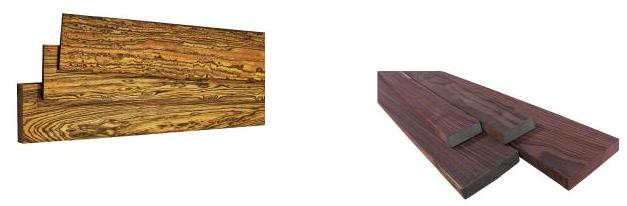
\includegraphics[width=0.5\textwidth]{optimization/multi-objective/images/2022_02_28_634e8079070800ac7e3cg-02}

The manufacturer has an ongoing deal with a foreign sawmill which supplies them with 960 and 200 board-feet (bdft) of bocote and rosewood respectively each month.

A single table requires 80 bdft of bocote and 20 bdft of rosewood.

Each chair requires only 20 bdft of bocote but 10 bdft of rosewood.
$$
\begin{aligned}
P=\{&(x, y) \in \mathbb{R}^{2}: \\
& 80 x+20 y \leq 960 \\
& 12 x+10 y \leq 200 \\
&x, y \geq 0\}
\end{aligned}
$$
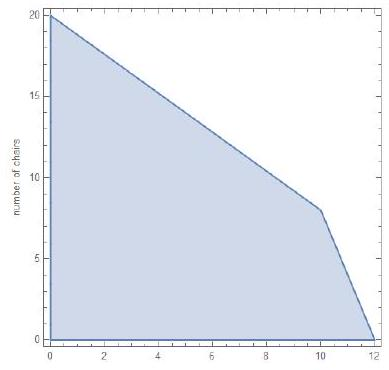
\includegraphics[width=0.5\textwidth]{optimization/multi-objective/images/2022_02_28_634e8079070800ac7e3cg-03}

Suppose that each table will sells for $\$ 7000$ while a chair goes for $\$ 1500 .$ To increase profit we want to maximize
$$
F(x, y)=8000 x+2000 y
$$
over $P$. Having taken a linear programming class, the manager knows his way around these problems and begins the simplex method:

Maximize $8000 x+2000 y$

s.t. $\quad 80 x+20 y \leq 960$
$$
12 x+10 y \leq 200
$$
$$
\begin{aligned}
& x, y \geq 0
\end{aligned}
$$
\begin{tabular}{llll|l}
$-4$ & $-1$ & 0 & 0 & 0 \\
\hline
4 & 1 & 1 & 0 & 48 \\
6 & 5 & 0 & 1 & 100 \\
\end{tabular}

Maximize $4 x+y$

s.t. $\quad 4 x+y+s_{1}=48$
$$
\begin{aligned}
& \begin{aligned}\frac{f}{2000} & \begin{aligned}6 x+5 y+s_{2} &=100 \\x, y & \geq 0\end{aligned}\end{aligned} 
\end{aligned}
$$
Having found an optimal solution, the manager is quick to set up production. The best thing to do is produce 12 tables a month and no chairs!

But there are actually multiple optima!

How could we have noticed this this from the tableau? From the original formulation?

Is the manager's solution really the best?

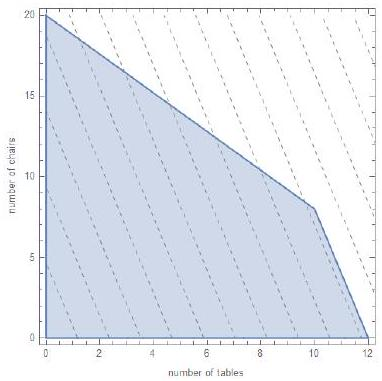
\includegraphics[width=0.5\textwidth]{optimization/multi-objective/images/2022_02_28_634e8079070800ac7e3cg-05}

number of tables Having fired the prior manager for producing no chairs, a new and more competent manager is hired. This one knows that Dalbergia stevensonii (the tree which produces their preferred rosewood) is a threatened species and decides that she doesn't want to waste any more rosewood than is necessary.

After some investigation, she finds that table production wastes nearly 10 bdft of rosewood per table while chairs are dramatically more efficient wasting only 2 bdft per chair. She comes up with a new, secondary objective function that she would like to minimize:
$$
w(x, y)=10 x+2 y .
$$
Having noticed that there are multiple profit-maximizers, she formulates a new problem to break the tie:
$$
\begin{aligned}
\text { Minimize } 10 x+2 y & \\
\text { s.t. } \quad 80 x+20 y &=960 \\
x & \in[10,12] \\
y & \in[0,8] .
\end{aligned}
$$
This is easy in this case because the set of profit-optimal solutions is simple.

Because this is an LP, the optimal solution will be at an extreme point; there are only two here, so the problem reduces to
$$
\arg \min \{10 x+2 y:(x, y) \in\{(12,0),(10,8)\}\}
$$
Therefore, swapping out some tables for chairs reduces waste and without affecting revenue!

What the manager just did is called the Ordered Criteria or Lexicographic method for Multi-Objective Optimization. After a few months, the manager convinces the owners that reducing waste is worth a small loss in profit. The owners concede to a $30 \%$ loss in revenue and our manager gets to work on a new model:
$$
\begin{aligned}
\text { Minimize } & 10 x+2 y \\
\text { s.t. } \quad 8000 x+2000 y & \geq(\alpha) 96000 \\
80 x+20 y & \leq 960 \\
12 x+10 y & \leq 200 \\
x, y & \geq 0
\end{aligned}
$$
where $\alpha=0.7$ This new constraint limits us to solutions which offered at least $70 \%$ of maximum possible revenue.

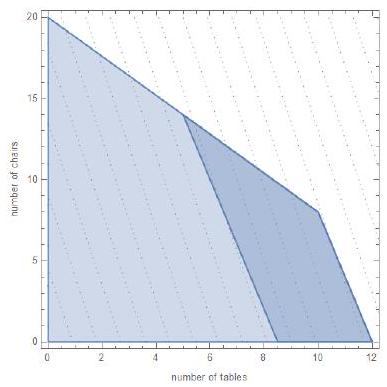
\includegraphics[width=0.5\textwidth]{optimization/multi-objective/images/2022_02_28_634e8079070800ac7e3cg-10}

The strategy is the called the Benchmark or Rollover method because we choose a benchmark for one of our objectives (revenue in this case), roll that benchmark into the constraints, and optimize for the second objective (waste).

Notice that if we set $\alpha$ to 1 , the rollover problem is equivalent to the lexicographic problem. Either approach requires a known optimal value to the first objective function.

Interestingly, our rollover solution is NOT an extreme point to the ORIGINAL feasible region. Given a set $P$ and some number of functions $f_{i}: P \rightarrow \mathbb{R}$ that we seek to maximize, we call a point $\mathbf{x} \in P$ Pareto Optimal or Efficient if there does not exist another point $\overline{\mathbf{x}} \in P$ such that

\begin{itemize}
  \item $f_{i}(\overline{\mathbf{x}})>f_{i}(\mathbf{x})$ for some $i$ and
\end{itemize}
$\rightarrow f_{j}(\overline{\mathbf{x}}) \geq f_{j}(\mathbf{x})$ for all $j \neq i$.

That is, we cannot make any objective better without making some other objective worse.

The Pareto Frontier is the set of all Pareto optimal points for some problem. Which of these points is Pareto optimal?

What is the frontier of this problem?

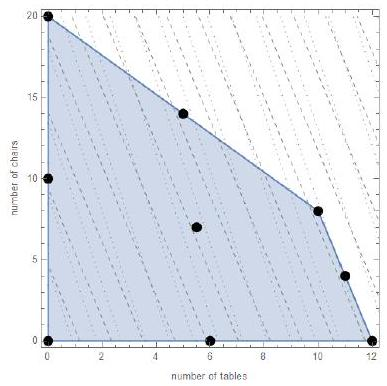
\includegraphics[width=0.5\textwidth]{optimization/multi-objective/images/2022_02_28_634e8079070800ac7e3cg-13}

number of tables The rollover method is generalized in Goal Programming

By varying $\alpha$, it is possible to generate many distinct efficient solutions.

However, this method can generate inefficient solutions if the underlying model is poorly constructed.

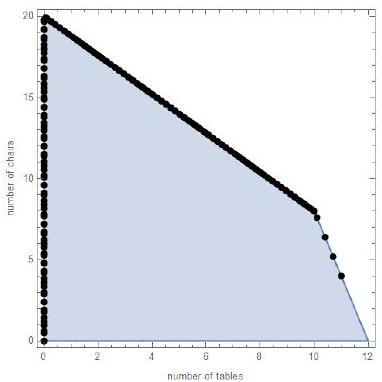
\includegraphics[width=0.5\textwidth]{optimization/multi-objective/images/2022_02_28_634e8079070800ac7e3cg-14}

number of tables It is more common to see a Pareto frontier plotted with respect to its objectives.

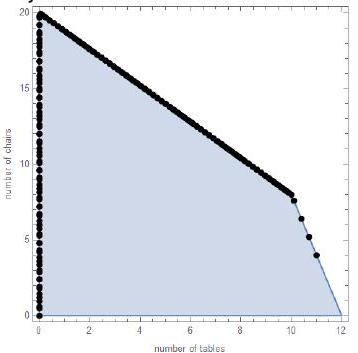
\includegraphics[width=0.5\textwidth]{optimization/multi-objective/images/2022_02_28_634e8079070800ac7e3cg-15}

number of table

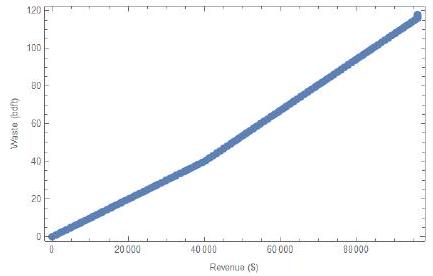
\includegraphics[width=0.5\textwidth]{optimization/multi-objective/images/2022_02_28_634e8079070800ac7e3cg-15(1)}

One of the owners of our manufactory decides to explore possible planning himself; he implements the multi-objective method that he remembers, Scalarization by picking some arbitrary constant $\lambda \in[0,1]$ and combining his two objectives like so:
$$
\begin{array}{cl}
\text { Minimize } & \lambda(8000 x+2000 y)+(1-\lambda)(10 x+2 y) \\
\text { s.t. } & 80 x+20 y \leq 960 \\
& 12 x+10 y \leq 200 \\
& x, y \geq 0
\end{array}
$$
What is the benefit of this method?

Where does it fall short?

\section{What points will the Scalarization method find if we vary $\lambda ?$}
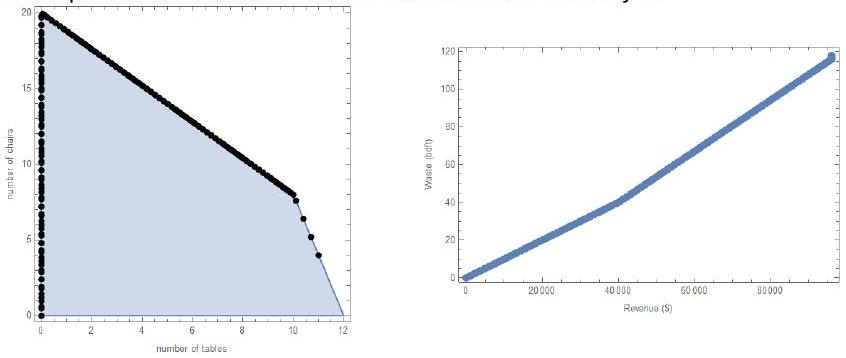
\includegraphics[width=0.5\textwidth]{optimization/multi-objective/images/2022_02_28_634e8079070800ac7e3cg-17}These are all nice ideas, but the problem presented above is neither difficult nor practical.

What are some areas that a Pareto frontier would be actually useful?

\section{Political Redistricting [3]}
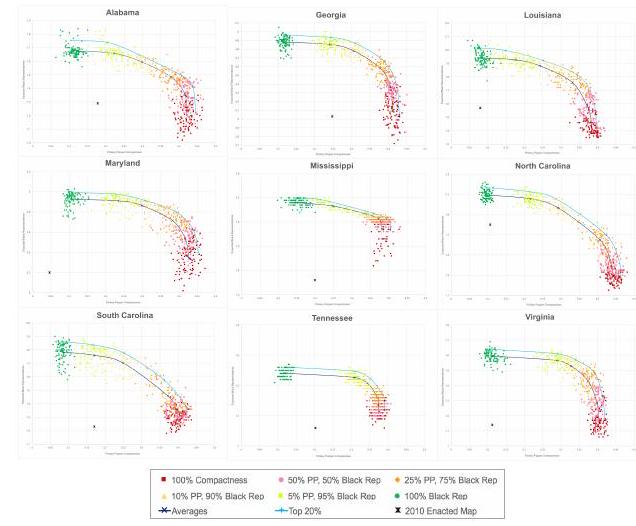
\includegraphics[width=0.5\textwidth]{optimization/multi-objective/images/2022_02_28_634e8079070800ac7e3cg-19}

\section{Portfolio Optimization [5]}
\section{Simulated Portfolio Optimization based on Efficient Frontier}
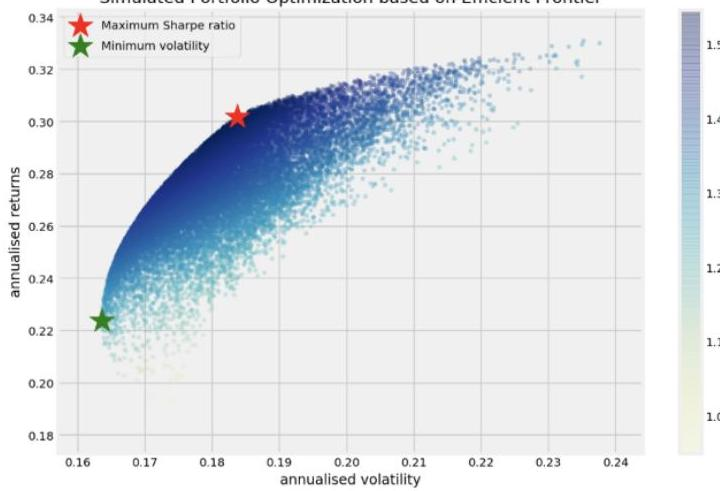
\includegraphics[width=0.5\textwidth]{optimization/multi-objective/images/2022_02_28_634e8079070800ac7e3cg-20}

\section{Aircraft Design [1]}
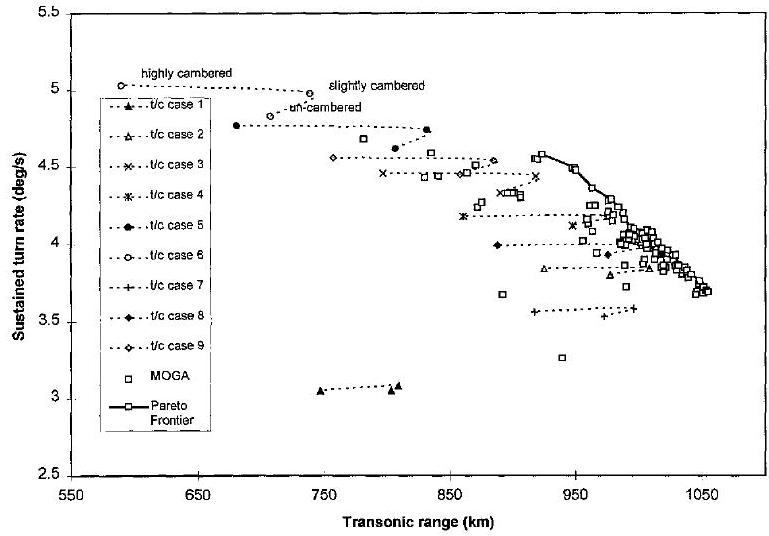
\includegraphics[width=0.5\textwidth]{optimization/multi-objective/images/2022_02_28_634e8079070800ac7e3cg-21}

\section{Vehicle Dynamics [4]}
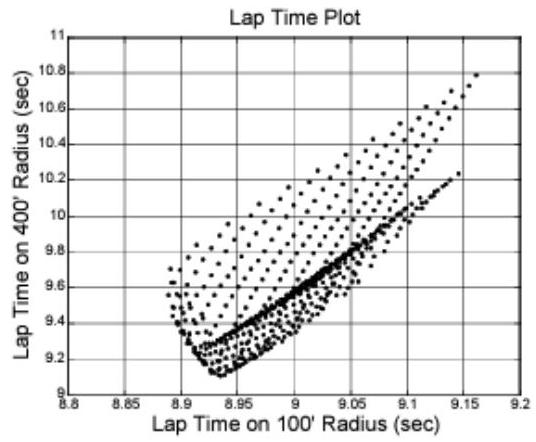
\includegraphics[width=0.5\textwidth]{optimization/multi-objective/images/2022_02_28_634e8079070800ac7e3cg-22}

Figure 7: Grid Search Results in the Performance Space

\section{Sustainable Constriction [2]}
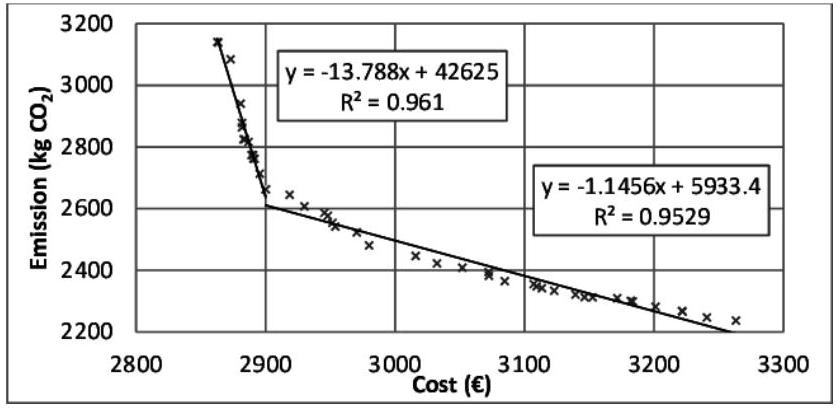
\includegraphics[width=0.5\textwidth]{optimization/multi-objective/images/2022_02_28_634e8079070800ac7e3cg-23}

\section{References}
S. Fenwick and John C. Harris. the application of pareto frontier methods in the multidisciplinary wing design of a generic modern military delta aircraft: Semantic scholar, Jan $1999 .$

URL: \href{https://WWW}{https://WWW}. semanticscholar. org/paper/

The-application-of-Pareto-frontier-methods-in-the-a-Fenwick-Harris/ fced $00 a 59 \mathrm{~d} 200 c 2 c 74$ ed 655 a 457344 bcleea 6 ff $5 .$

T García-Segura, V Yepes, and J Alcalá.

Sustainable design using multiobjective optimization of high-strength concrete i-beams. In The 2014 International Conference on High Performance and Optimum Design of Structures and Materials HPSM/OPTI, volume 137, pages $347-358,2014 .$

URL: \href{https://www}{https://www}. \href{http://researchgate.net/publication/271439836_Sustainable_design_using_}{researchgate.net/publication/271439836\_Sustainable\_design\_using\_} multiobjective\_optimization\_of\_high-strength\_concrete\_l-beams.

Nicholas Goedert, Robert Hildebrand, Laurel Travis, Matthew Pierson, and Jamie Fravel. Black representation and district compactness in southern congressional districts. not yet published, ask Dr. Hildebrand for it.

Edward M Kasprzak and Kemper E Lewis.

Pareto analysis in multiobjective optimization using the collinearity theorem and scaling method. Structural and Multidisciplinary Optimization.

Ricky Kim.

Efficient frontier portfolio optimisation in python, Jun $2021 .$

URL: \href{https://towardsdatascience}{https://towardsdatascience}. com/

efficient-frontier-portfolio-optimisation-in-python-e7844051e7f.


%\end{document}

\part{Discrete Algorithms}

\chapter{Graph Algorithms}
\todoChapter{ {\color{gray}10\% complete. Goal 80\% completion date: August 20}\\
Notes: .}

% Copyright 2022 by Robert Hildebrand
%This work is licensed under a
%Creative Commons Attribution-ShareAlike 4.0 International License (CC BY-SA 4.0)
%See http://creativecommons.org/licenses/by-sa/4.0/



\todo[inline]{Write this section.}



\newcommand{\sout}{}

\section{Graph Theory and Network Flows}
In the modern world, planning efficient routes is essential for business and industry, with applications as varied as product distribution, laying new fiber optic lines for broadband internet, and suggesting new friends within social network websites like Facebook.

This field of mathematics started nearly 300 years ago as a look into a mathematical puzzle (we'll look at it in a bit).  The field has exploded in importance in the last century, both because of the growing complexity of business in a global economy and because of the computational power that computers have provided us.  
\section{Graphs}
\subsection{Drawing Graphs}

\begin{example}{}{}
Here is a portion of a housing development from Missoula, Montana\footnote{Same Beebe. http://www.flickr.com/photos/sbeebe/2850476641/}.  As part of her job, the development's lawn inspector has to walk down every street in the development making sure homeowners' landscaping conforms to the community requirements.\\
\begin{center}
\scalebox{0.8}{
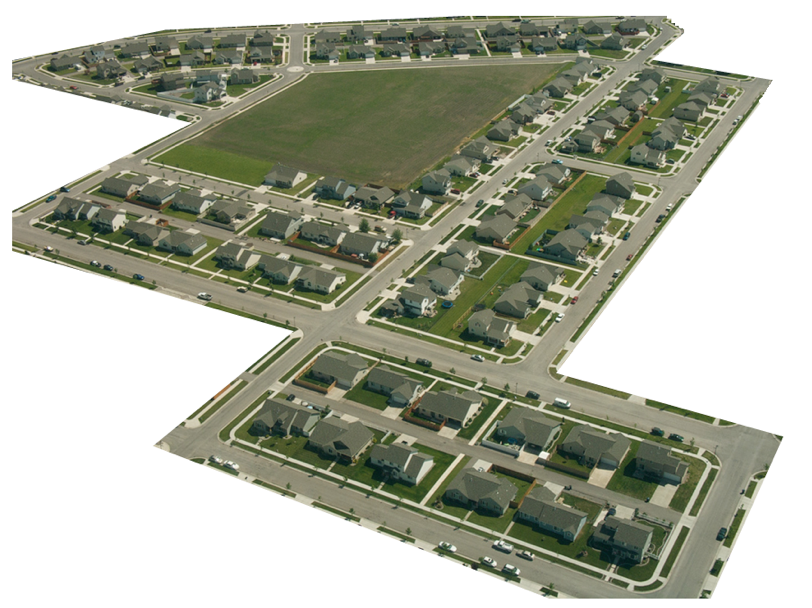
\includegraphics{graph-theory-graphics/GraphPicture.png}
}
\end{center}

Naturally, she wants to minimize the amount of walking she has to do.  Is it possible for her to walk down every street in this development without having to do any backtracking?  While you might be able to answer that question just by looking at the picture for a while, it would be ideal to be able to answer the question for any picture regardless of its complexity.\\

To do that, we first need to simplify the picture into a form that is easier to work with.  We can do that by drawing a simple line for each street.  Where streets intersect, we will place a dot. \\
 
 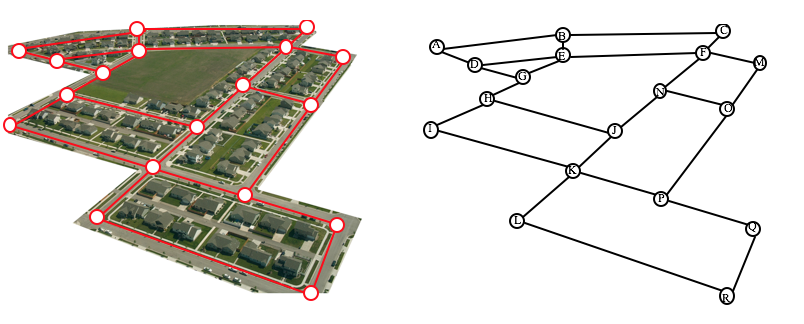
\includegraphics{graph-theory-graphics/GraphPictureDot.png}
\end{example}

This type of simplified picture is called a \textbf{graph}.  


\begin{definition}{Graphs, Vertices, and Edges}{}
A graph consists of a set of dots, called vertices, and a set of edges connecting pairs of vertices.  
\end{definition}

While we drew our original graph to correspond with the picture we had, there is nothing particularly important about the layout when we analyze a graph.  Both of the graphs below are equivalent to the one drawn above since they show the same edge connections between the same vertices as the original graph.

 
\begin{minipage}{0.5\textwidth}
\begin{tikzpicture}
    \foreach \pos/\name in {{(0,0)/A}, {(1,0)/D}, {(2,0)/G}, {(3,0)/N}, {(4,0)/O}, {(1,1)/B}, {(2,1)/E}, {(3,1)/F}, {(4,1)/M}, {(3,2)/C}, {(2,-1)/H}, {(3,-1)/J}, {(2,-2)/I}, {(3,-2)/K}, {(4,-2)/P}, {(5,-2)/Q}, {(3,-3)/L}, {(5,-3)/R}}
                \node[vertex] (\name) at \pos {$\name$};
                
 \foreach \source/ \dest in {A/D, D/G, A/B, B/E, B/C, C/F, E/F, F/M, D/E, E/G, G/H, H/I, H/J, I/K, J/K, K/L, N/J, F/N, F/M, N/O, O/P, P/Q, Q/R, M/O, K/P, L/R}
              \path (\source) edge (\dest);                
\end{tikzpicture}     
\end{minipage}
%
\begin{minipage}{0.5\textwidth}
\begin{tikzpicture}
    \foreach \pos/\name in {{(0,0)/A}, {(0,-1)/D}, {(0.6,-2.25)/G}, {(6,-1)/N}, {(3.5,2.5)/O}, {(.25,1)/B}, {(5.4,1.25)/E}, {(2.4,-3.5)/F}, {(4.6,2.25)/M}, {(1,1.75)/C}, {(1.4,-3.25)/H}, {(5.75,-2)/J}, {(6,0)/I}, {(3.5,-3.5)/K}, {(2.5,2.5)/P}, {(1.6,2.25)/Q}, {(4.4,-3.25)/L}, {(5,-2.75)/R}}
                \node[vertex] (\name) at \pos {$\name$};
                
 \foreach \source/ \dest in {A/D, D/G, A/B, B/E, B/C, C/F, E/F, F/M, D/E, E/G, G/H, H/I, H/J, I/K, J/K, K/L, N/J, F/N, F/M, N/O, O/P, P/Q, Q/R, M/O, K/P, L/R}
              \path (\source) edge (\dest);                
\end{tikzpicture}   
\end{minipage}

You probably already noticed that we are using the term graph differently than you may have used the term in the past to describe the graph of a mathematical function.


\begin{example}{}{}

Back in the 18th century in the Prussian city of K\"onigsberg, a river ran through the city and seven bridges crossed the forks of the river.  The river and the bridges are highlighted in the picture to the right%\footnote{Bogdan Giusc\u{a}. \url{http://en.wikipedia.org/wiki/File:Konigsberg\_bridges.png}}.

\textcolor{red}{Picture}

As a weekend amusement, townsfolk would see if they could find a route that would take them across every bridge once and return them to where they started.

Leonard Euler (pronounced OY-lur), one of the most prolific mathematicians ever, looked at this problem in 1735, laying the foundation for graph theory as a field in mathematics.  To analyze this problem, Euler introduced edges representing the bridges:
\begin{center}
\begin{tikzpicture}
\draw (2,2) ellipse (4cm and .9cm); %NB
\node at (2,2) {North Bank};
\draw (-1,0) ellipse (1.5cm and .9cm); %I
\node at (-1,0) {Island};
\draw (6,0) ellipse (2cm and .9cm); %EB
\node at (6,0) {East Bank};
\draw (1,-2) ellipse (3cm and .9cm);
\node at (1,-2) {South Bank};
\draw(-1.1,.9)--(-.9,1.4);
\draw(-.6,.85)--(-.1,1.25);
\draw(-1.1,-.9)--(-.9,-1.3);
\draw(-.6,-.85)--(-.1,-1.15);
\draw(0.5,0)--(4,0);
\draw(5.6,0.9)--(5.2,1.45);
\draw(5.61,-0.9)--(3.8,-1.7);
\end{tikzpicture}
\end{center}
Since the size of each land mass it is not relevant to the question of bridge crossings, each can be shrunk down to a vertex representing the location:
\begin{center}
\begin{tikzpicture}
\draw(0,1)--(2,1);
\draw(0,2)--(2,1);
\draw(0,0)--(2,1);
\draw(0,0) to [out=40] (0.1,1);
\draw(0,0) to [out=135] (0.1,1);
\draw(0,1) to [out=40] (0.1,2);
\draw(0,1) to [out=135] (0.1,2);
\draw[fill] (0,0) circle[radius=.1] node [left]{SB};
\draw[fill] (0,1) circle[radius=.1] node [left]{I   };
\draw[fill] (0,2) circle[radius=.1] node [left]{NB};
\draw[fill] (2,1) circle[radius=.1] node [right]{EB};
\end{tikzpicture}
\end{center}

Notice that in this graph there are \textit{two} edges connecting the north bank and island, corresponding to the two bridges in the original drawing.  Depending upon the interpretation of edges and vertices appropriate to a scenario, it is entirely possible and reasonable to have more than one edge connecting two vertices.

While we haven't answered the actual question yet of whether or not there is a route which crosses every bridge once and returns to the starting location, the graph provides the foundation for exploring this question.
 \end{example}


\section{Definitions}
While we loosely defined some terminology earlier, we now will try to be more specific.

\begin{definition}{Vertex}{vertex} 
A vertex is a dot in the graph that could represent an intersection of streets, a land mass, or a general location, like ``work? or ``school".  Vertices are often connected by edges.  Note that vertices only occur when a dot is explicitly placed, not whenever two edges cross.  Imagine a freeway overpass -- the freeway and side street cross, but it is not possible to change from the side street to the freeway at that point, so there is no intersection and no vertex would be placed.
\end{definition}

\begin{definition}{Edges}{}
Edges connect pairs of vertices.  An edge can represent a physical connection between locations, like a street, or simply that a route connecting the two locations exists, like an airline flight.
\end{definition}

\begin{definition}{Loop}{}
A loop is a special type of edge that connects a vertex to itself.  Loops are not used much in street network graphs.\\

\begin{tikzpicture}
\draw[fill] (0,0) circle[radius=.1];
\draw[fill] (1,-1) circle[radius=.1];
\draw[fill] (1.5,0) circle[radius=.1];
\draw(0,0)--(1,-1);
\draw(0,0)--(1.5,0);
\draw(1.5,0)--(1,-1);  
 \draw[red](1.5,0) to [out=90] (2,0);
 \draw[red](1.5,0) to [out=-90, in=-90] (2,0);
 \end{tikzpicture}
 \end{definition}


\begin{definition}{Degree of a vertex}{}
The degree of a vertex is the number of edges meeting at that vertex.  It is possible for a vertex to have a degree of zero or larger.
\begin{center}
\begin{tabular}{|c|c|c|c|c|}
\hline
Degree 0 & Degree 1 & Degree 2 & Degree 3 & Degree 4\\
\hline
\begin{tikzpicture}
\draw[fill] (0,0) circle[radius=.1];
\node at (0,-1){};
\end{tikzpicture}
&
\begin{tikzpicture}
\draw[fill] (0,0) circle[radius=.1];
\draw(0,0)--(1,1);
\node at (-.6,-1){};
\node at (1,1){};
\end{tikzpicture}
&
\begin{tikzpicture}
\draw[fill] (0,0) circle[radius=.1];
\draw(0,0)--(1,1);
\draw(0,0)--(1,-1);
\end{tikzpicture}
&
\begin{tikzpicture}
\draw[fill] (0,0) circle[radius=.1];
\draw(0,0)--(1,1);
\draw(0,0)--(1,-1);
\draw(0,0)--(-1,1);
\end{tikzpicture}
&
\begin{tikzpicture}
\draw[fill] (0,0) circle[radius=.1];
\draw(0,0)--(1,1);
\draw(0,0)--(1,-1);
\draw(0,0)--(-1,1);
\draw(0,0)--(-1,-1);
\end{tikzpicture}\\
\hline
\end{tabular}
\end{center}
 
 \end{definition}



\begin{definition}{Path}{}
A path is a sequence of vertices using the edges.  Usually we are interested in a path between two vertices.  For example, a path from vertex A to vertex M is shown below.  It is one of many possible paths in this graph. 

\begin{tikzpicture}
\draw[fill] (0,2) circle[radius=.1] node[above]{A};
\draw[fill] (1,2) circle[radius=.1] node[above]{B};
\draw[fill] (2,2) circle[radius=.1] node[above]{C};
\draw[fill] (3,2) circle[radius=.1] node[above]{D};
\draw[fill] (0,1) circle[radius=.1];
\node at (0.3,1.3){E}; 
\draw[fill] (1,1) circle[radius=.1];
\node at (1.3,1.3){F}; 
\draw[fill] (2,1) circle[radius=.1];
\node at (2.3,1.3){G};  
\draw[fill] (3,1) circle[radius=.1];
\node at (3.3,1.3){H};  
\draw[fill] (0,0) circle[radius=.1] node[below]{J};
\draw[fill] (1,0) circle[radius=.1] node[below]{K};
\draw[fill] (2,0) circle[radius=.1] node[below]{L};
\draw[fill] (3,0) circle[radius=.1] node[below]{M};
\draw(0,0)--(0,1);
\draw[very thick, red](0,1)--(0,2);
\draw(1,0)--(1,1);
\draw(1,1)--(1,2);
\draw[very thick, red](2,0)--(2,1);
\draw(2,1)--(2,2);
\draw(3,0)--(3,1);
\draw(3,1)--(3,2);
\draw(0,0)--(1,0);
\draw(1,0)--(2,0);
\draw[very thick, red](2,0)--(3,0);
\draw[very thick, red](0,1)--(1,1);
\draw[very thick, red](1,1)--(2,1);
\draw(2,1)--(3,1);
\draw(0,2)--(1,2);
\draw(1,2)--(2,2);
\draw(2,2)--(3,2);
\end{tikzpicture}

 \end{definition}



\begin{definition}{Circuit (a.k.a. cycle)}{}
A circuit  (a.k.a. cycle) is a path that begins and ends at the same vertex.  A circuit  (a.k.a. cycle) starting and ending at vertex A is shown below.

\begin{tikzpicture}
\draw[fill] (0,2) circle[radius=.1] node[above]{A};
\draw[fill] (1,2) circle[radius=.1] node[above]{B};
\draw[fill] (2,2) circle[radius=.1] node[above]{C};
\draw[fill] (3,2) circle[radius=.1] node[above]{D};
\draw[fill] (0,1) circle[radius=.1];
\node at (0.3,1.3){E}; 
\draw[fill] (1,1) circle[radius=.1];
\node at (1.3,1.3){F}; 
\draw[fill] (2,1) circle[radius=.1];
\node at (2.3,1.3){G};  
\draw[fill] (3,1) circle[radius=.1];
\node at (3.3,1.3){H};  
\draw[fill] (0,0) circle[radius=.1] node[below]{J};
\draw[fill] (1,0) circle[radius=.1] node[below]{K};
\draw[fill] (2,0) circle[radius=.1] node[below]{L};
\draw[fill] (3,0) circle[radius=.1] node[below]{M};
\draw[very thick, red](0,0)--(0,1);
\draw[very thick, red](0,1)--(0,2);
\draw(1,0)--(1,1);
\draw[very thick, red](1,1)--(1,2);
\draw[very thick, red](2,0)--(2,1);
\draw(2,1)--(2,2);
\draw(3,0)--(3,1);
\draw(3,1)--(3,2);
\draw[very thick, red](0,0)--(1,0);
\draw[very thick, red](1,0)--(2,0);
\draw(2,0)--(3,0);
\draw(0,1)--(1,1);
\draw[very thick, red](1,1)--(2,1);
\draw(2,1)--(3,1);
\draw[very thick, red](0,2)--(1,2);
\draw(1,2)--(2,2);
\draw(2,2)--(3,2);
\end{tikzpicture}

\end{definition}




\begin{definition}{Connected}{}
A graph is connected if there is a path from any vertex to any other vertex.  Every graph drawn so far has been connected.  The graph below is \textbf{disconnected}; there is no way to get from the vertices on the left to the vertices on the right.

\begin{tikzpicture}
\draw[fill] (0,2) circle[radius=.1] node[above]{A};
\draw[fill] (1,2) circle[radius=.1] node[above]{B};
\draw[fill] (2,2) circle[radius=.1] node[above]{C};
\draw[fill] (3,2) circle[radius=.1] node[above]{D};
\draw[fill] (0,1) circle[radius=.1];
\node at (0.3,1.3){E}; 
\draw[fill] (1,1) circle[radius=.1];
\node at (1.3,1.3){F}; 
\draw[fill] (2,1) circle[radius=.1];
\node at (2.3,1.3){G};  
\draw[fill] (3,1) circle[radius=.1];
\node at (3.3,1.3){H};  
\draw[fill] (0,0) circle[radius=.1] node[below]{J};
\draw[fill] (1,0) circle[radius=.1] node[below]{K};
\draw[fill] (2,0) circle[radius=.1] node[below]{L};
\draw[fill] (3,0) circle[radius=.1] node[below]{M};
\draw(0,0)--(0,1);
\draw(1,0)--(1,1);
\draw(1,1)--(1,2);
\draw(2,0)--(2,1);
\draw(2,1)--(2,2);
\draw(3,0)--(3,1);
\draw(3,1)--(3,2);
\draw(2,0)--(3,0);
\draw(0,1)--(1,1);

\draw(2,1)--(3,1);
\draw(0,2)--(1,2);
\draw(2,2)--(3,2);
\end{tikzpicture}
 \end{definition}





\begin{definition}{Weights}{}
Depending upon the problem being solved, sometimes weights are assigned to the edges.  The weights could represent the distance between two locations, the travel time, or the travel cost.  It is important to note that the distance between vertices in a graph does not necessarily correspond to the weight of an edge.
 \end{definition}

\begin{exercise}{}{}
The graph below shows 5 cities.  The weights on the edges represent the airfare for a one-way flight between the cities.
 \begin{enumerate}[label=\alph*.]
 \item How many vertices and edges does the graph have?
 \item Is the graph connected?
 \item What is the degree of the vertex representing LA?
 \item If you fly from Seattle to Dallas to Atlanta, is that a path or a circuit?
 \item If you fly from LA to Chicago to Dallas to LA, is that a path or a circuit?
 \end{enumerate}
 
 \begin{tikzpicture}
 \draw[fill] (0,0) circle[radius=.1] node[left]{LA};
\draw[fill] (2,-2) circle[radius=.1] node[below]{Chicago};
\draw[fill] (4,2) circle[radius=.1] node[above]{Seattle};
\draw[fill] (6,-2) circle[radius=.1] node[below]{Atlanta};
\draw[fill] (8,0) circle[radius=.1] node[right]{Dallas};
\draw(0,0)--(2,-2);
\node at (0.5,-1){\$100};
\draw(0,0)--(4,2);
\node at (1.4,1){\$70};
\draw(0,0)--(8,0);
\node at (4,0.3){\$150};
\draw(0,0)--(6,-2);
\node at (3.2,-0.7){\$170};
\draw(2,-2)--(4,2);
\node at (3.15,1.2){\$145};
\draw(4,2)--(6,-2);
\node at (4.8, 1.2){\$140};
\draw(4,2)--(8,0);
\node at (6.7,1){\$120};
\draw(2,-2)--(8,0);
\node at (6,-1){\$165};
\draw(2,-2)--(6,-2);
\node at (4,-2.3){\$75};
\draw(6,-2)--(8,0);
\node at (7.5,-1){\$85};
 \end{tikzpicture}
 \end{exercise}


\section{Shortest Path}
\begin{outcome}
\begin{itemize}
\item What is the problem statement?
\item How to use Dijkstra's algorihtm
\item Software solutions
\end{itemize}
\end{outcome}
\begin{resource}
\begin{itemize}
\item \href{https://youtu.be/EFg3u_E6eHU}{YouTube Video of Dijkstra's Algorithm}
\item \href{https://github.com/open-optimization/open-optimization-or-book/blob/master/instructive-code/networkx%20example%20-%20Dijkstra's%20Algorithm.ipynb}{Python Example using Networkx and also showing Dijkstra's algorithm}
\end{itemize}
\end{resource}
When you visit a website like Google Maps or use your Smartphone to ask for directions from home to your Aunt's house in Pasadena, you are usually looking for a shortest path between the two locations.  These computer applications use representations of the street maps as graphs, with estimated driving times as edge weights.

While often it is possible to find a shortest path on a small graph by guess-and-check, our goal in this chapter is to develop methods to solve complex problems in a systematic way by following \textbf{algorithms}.  An algorithm is a step-by-step procedure for solving a problem.  Dijkstra's (pronounced dike-stra) algorithm will find the shortest path between two vertices.


%\begin{algorithm}{Dijkstra's Algorithm}{}{}
{\Large \textbf{Dijkstra's Algorithm} } \\
\hspace{3in}

\begin{enumerate}
\item	Mark the ending vertex with a distance of zero.  Designate this vertex as current.
\item Find all vertices leading to the current vertex.  Calculate their distances to the end.  Since we already know the distance the current vertex is from the end, this will just require adding the most recent edge.  Don't record this distance if it is longer than a previously recorded distance.
\item	Mark the current vertex as visited.  We will never look at this vertex again.
\item	Mark the vertex with the smallest distance as current, and repeat from step 2.
\end{enumerate}
 %\end{algorithm}

\newpage
\begin{example}{}{}
Suppose you need to travel from Yakima, WA (vertex Y) to Tacoma, WA (vertex T)  Looking at a map, it looks like driving through Auburn (A) then Mount Rainier (MR) might be shortest, but it's not totally clear since that road is probably slower than taking the major highway through North Bend (NB).  A graph with travel times in minutes is shown below.  An alternate route through Eatonville (E) and Packwood (P) is also shown.

\begin{tikzpicture}
\draw[fill] (0,0) circle[radius=.1] node[left]{T};
\draw[fill] (2,-2) circle[radius=.1] node[left]{E};
\draw[fill] (2,1) circle[radius=.1];
\node at (1.7,1.2){A};
\draw[fill] (4,2) circle[radius=.1]; 
\node at (3.6,2.2){NB};
\draw[fill] (4,0) circle[radius=.1];
\node at (4.05,0.3){MR};
\draw[fill] (4,-1) circle[radius=.1];
\node at (4.3,-1.2){P};
\draw[fill] (8,0) circle[radius=.1] node[right]{Y};
\draw(0,0)--(2,-2);
\node at (0.6,-1){57};
\draw(0,0)--(2,1);
\node at (0.5, 0.5){20};
\draw(2,1)--(4,2);
\node at (2.5,1.5){36};
\draw(4,2)--(8,0);
\node at (6,1.3){104};
\draw(2,-2)--(4,-1);
\node at (3,-1.8){96};
\draw(4,-1)--(8,0);
\node at (6,-0.7){76};
\draw(2,1)--(4,0);
\node at (3.1,0.7){79};
\draw(4,0)--(4,-1);
\node at (3.7, -0.5){27};
\draw(4,0)--(8,0);
\node at (6,0.3){96};
\end{tikzpicture}







\noindent Step 1:  Mark the ending vertex with a distance of zero.  The distances will be recorded in [brackets] after the vertex name.\\
\begin{tikzpicture}
\draw[fill] (0,0) circle[radius=.1] node[left]{T};
\draw[fill] (2,-2) circle[radius=.1] node[left]{E};
\draw[fill] (2,1) circle[radius=.1];
\node at (1.7,1.2){A};
\draw[fill] (4,2) circle[radius=.1]; 
\node at (3.6,2.2){NB};
\draw[fill] (4,0) circle[radius=.1];
\node at (4.05,0.3){MR};
\draw[fill] (4,-1) circle[radius=.1];
\node at (4.3,-1.2){P};
\draw[fill] (8,0) circle[radius=.1] node[right]{Y\textcolor{red}{[0]}};
\draw(0,0)--(2,-2);
\node at (0.6,-1){57};
\draw(0,0)--(2,1);
\node at (0.5, 0.5){20};
\draw(2,1)--(4,2);
\node at (2.5,1.5){36};
\draw(4,2)--(8,0);
\node at (6,1.3){104};
\draw(2,-2)--(4,-1);
\node at (3,-1.8){96};
\draw(4,-1)--(8,0);
\node at (6,-0.7){76};
\draw(2,1)--(4,0);
\node at (3.1,0.7){79};
\draw(4,0)--(4,-1);
\node at (3.7, -0.5){27};
\draw(4,0)--(8,0);
\node at (6,0.3){96};
\end{tikzpicture}


\noindent Step 2:  For each vertex leading to Y, we calculate the distance to the end.  For example, NB is a distance of 104 from the end, and MR is 96 from the end.  Remember that distances in this case refer to the travel time in minutes.\\
\begin{tikzpicture}
\draw[fill] (0,0) circle[radius=.1] node[left]{T};
\draw[fill] (2,-2) circle[radius=.1] node[left]{E};
\draw[fill] (2,1) circle[radius=.1];
\node at (1.7,1.2){A};
\draw[fill] (4,2) circle[radius=.1]; 
\node at (3.6,2.3){NB\textcolor{red}{[104]}};
\draw[fill] (4,0) circle[radius=.1];
\node at (4.3,0.3){MR\textcolor{red}{[96]}};
\draw[fill] (4,-1) circle[radius=.1];
\node at (4.6,-1.2){P\textcolor{red}{[76]}};
\draw[fill] (8,0) circle[radius=.1] node[right]{Y\textcolor{red}{[0]}};
\draw(0,0)--(2,-2);
\node at (0.6,-1){57};
\draw(0,0)--(2,1);
\node at (0.5, 0.5){20};
\draw(2,1)--(4,2);
\node at (2.5,1.5){36};
\draw(4,2)--(8,0);
\node at (6,1.3){104};
\draw(2,-2)--(4,-1);
\node at (3,-1.8){96};
\draw(4,-1)--(8,0);
\node at (6,-0.7){76};
\draw(2,1)--(4,0);
\node at (3.1,0.7){79};
\draw(4,0)--(4,-1);
\node at (3.7, -0.5){27};
\draw(4,0)--(8,0);
\node at (6,0.3){96};
\end{tikzpicture}


\noindent Step 3 \& 4:  We mark Y as visited, and mark the vertex with the smallest recorded distance as current.  At this point, P will be designated current.  Back to step 2.\\

\newpage
\noindent Step 2 (\#2):  For each vertex leading to P (and not leading to a visited vertex) we find the distance from the end.  Since E is 96 minutes from P, and we've already calculated P is 76 minutes from Y, we can compute that E is $96+76 = 172$ minutes from Y.  \\

If we make the same computation for MR, we'd calculate $76+27 = 103$.  Since this is larger than the previously recorded distance from Y to MR, we will not replace it.\\
\begin{tikzpicture}
\draw[fill] (0,0) circle[radius=.1] node[left]{T};
\draw[fill] (2,-2) circle[radius=.1] node[left]{E\textcolor{red}{[172]}};
\draw[fill] (2,1) circle[radius=.1];
\node at (1.7,1.2){A};
\draw[fill] (4,2) circle[radius=.1]; 
\node at (3.6,2.3){NB\textcolor{red}{[104]}};
\draw[fill] (4,0) circle[radius=.1];
\node at (4.3,0.3){MR\textcolor{red}{[96]}};
\draw[fill] (4,-1) circle[radius=.1];
\node at (4.6,-1.2){P\textcolor{red}{[76]}};
\draw[fill] (8,0) circle[radius=.1] node[right]{\textcolor{gray}{\sout{Y}}\textcolor{red}{[0]}};
\draw(0,0)--(2,-2);
\node at (0.6,-1){57};
\draw(0,0)--(2,1);
\node at (0.5, 0.5){20};
\draw(2,1)--(4,2);
\node at (2.5,1.5){36};
\draw(4,2)--(8,0);
\node at (6,1.3){104};
\draw(2,-2)--(4,-1);
\node at (3,-1.8){96};
\draw(4,-1)--(8,0);
\node at (6,-0.7){76};
\draw(2,1)--(4,0);
\node at (3.1,0.7){79};
\draw(4,0)--(4,-1);
\node at (3.7, -0.5){27};
\draw(4,0)--(8,0);
\node at (6,0.3){96};
\end{tikzpicture}



\noindent Step 3 \& 4 (\#2):  We mark P as visited, and designate the vertex with the smallest recorded distance as current:  MR.  Back to step 2.\\

\noindent Step 2 (\#3):  For each vertex leading to MR (and not leading to a visited vertex) we find the distance to the end.  The only vertex to be considered is A, since we've already visited Y and P.  Adding MR's distance 96 to the length from A to MR gives the distance $96+79 = 175$ minutes from A to Y.  \\
\begin{tikzpicture}
\draw[fill] (0,0) circle[radius=.1] node[left]{T};
\draw[fill] (2,-2) circle[radius=.1] node[left]{E\textcolor{red}{[172]}};
\draw[fill] (2,1) circle[radius=.1];
\node at (1.5,1.2){A\textcolor{red}{[175]}};
\draw[fill] (4,2) circle[radius=.1]; 
\node at (3.6,2.3){NB\textcolor{red}{[104]}};
\draw[fill] (4,0) circle[radius=.1];
\node at (4.3,0.3){MR\textcolor{red}{[96]}};
\draw[fill] (4,-1) circle[radius=.1];
\node at (4.6,-1.2){\textcolor{gray}{\sout{P}}\textcolor{red}{[76]}};
\draw[fill] (8,0) circle[radius=.1] node[right]{\textcolor{gray}{\sout{Y}}\textcolor{red}{[0]}};
\draw(0,0)--(2,-2);
\node at (0.6,-1){57};
\draw(0,0)--(2,1);
\node at (0.5, 0.5){20};
\draw(2,1)--(4,2);
\node at (2.5,1.5){36};
\draw(4,2)--(8,0);
\node at (6,1.3){104};
\draw(2,-2)--(4,-1);
\node at (3,-1.8){96};
\draw(4,-1)--(8,0);
\node at (6,-0.7){76};
\draw(2,1)--(4,0);
\node at (3.1,0.7){79};
\draw(4,0)--(4,-1);
\node at (3.7, -0.5){27};
\draw(4,0)--(8,0);
\node at (6,0.3){96};
\end{tikzpicture}


\noindent Step 3 \& 4 (\#3):  We mark MR as visited, and designate the vertex with smallest recorded distance as current: NB.  Back to step 2.\\

\noindent Step 2 (\#4):  For each vertex leading to NB, we find the distance to the end.  We know the shortest distance from NB to Y is 104 and the distance from A to NB is 36, so the distance from A to Y through NB is $104+36 = 140$.  Since this distance is shorter than the previously calculated distance from Y to A through MR, we replace it.\\
\begin{tikzpicture}
\draw[fill] (0,0) circle[radius=.1] node[left]{T};
\draw[fill] (2,-2) circle[radius=.1] node[left]{E\textcolor{red}{[172]}};
\draw[fill] (2,1) circle[radius=.1];
\node at (1.5,1.2){A\textcolor{red}{[140]}};
\draw[fill] (4,2) circle[radius=.1]; 
\node at (3.6,2.3){NB\textcolor{red}{[104]}};
\draw[fill] (4,0) circle[radius=.1];
\node at (4.3,0.3){\textcolor{gray}{\sout{MR}}\textcolor{red}{[96]}};
\draw[fill] (4,-1) circle[radius=.1];
\node at (4.6,-1.2){\textcolor{gray}{\sout{P}}\textcolor{red}{[76]}};
\draw[fill] (8,0) circle[radius=.1] node[right]{\textcolor{gray}{\sout{Y}}\textcolor{red}{[0]}};
\draw(0,0)--(2,-2);
\node at (0.6,-1){57};
\draw(0,0)--(2,1);
\node at (0.5, 0.5){20};
\draw(2,1)--(4,2);
\node at (2.5,1.5){36};
\draw(4,2)--(8,0);
\node at (6,1.3){104};
\draw(2,-2)--(4,-1);
\node at (3,-1.8){96};
\draw(4,-1)--(8,0);
\node at (6,-0.7){76};
\draw(2,1)--(4,0);
\node at (3.1,0.7){79};
\draw(4,0)--(4,-1);
\node at (3.7, -0.5){27};
\draw(4,0)--(8,0);
\node at (6,0.3){96};
\end{tikzpicture}

\noindent Step 3 \& 4 (\#4):  We mark NB as visited, and designate A as current, since it now has the shortest distance.\\


\noindent Step 2 (\#5):  T is the only non-visited vertex leading to A, so we calculate the distance from T to Y through A:  $20+140 = 160$ minutes.  \\
\begin{tikzpicture}
\draw[fill] (0,0) circle[radius=.1] node[left]{T\textcolor{red}{[160]}};
\draw[fill] (2,-2) circle[radius=.1] node[left]{E\textcolor{red}{[172]}};
\draw[fill] (2,1) circle[radius=.1];
\node at (1.5,1.2){A\textcolor{red}{[140]}};
\draw[fill] (4,2) circle[radius=.1]; 
\node at (3.6,2.3){\textcolor{gray}{\sout{NB}}\textcolor{red}{[104]}};
\draw[fill] (4,0) circle[radius=.1];
\node at (4.3,0.3){\textcolor{gray}{\sout{MR}}\textcolor{red}{[96]}};
\draw[fill] (4,-1) circle[radius=.1];
\node at (4.6,-1.2){\textcolor{gray}{\sout{P}}\textcolor{red}{[76]}};
\draw[fill] (8,0) circle[radius=.1] node[right]{\textcolor{gray}{\sout{Y}}\textcolor{red}{[0]}};
\draw(0,0)--(2,-2);
\node at (0.6,-1){57};
\draw(0,0)--(2,1);
\node at (0.5, 0.5){20};
\draw(2,1)--(4,2);
\node at (2.5,1.5){36};
\draw(4,2)--(8,0);
\node at (6,1.3){104};
\draw(2,-2)--(4,-1);
\node at (3,-1.8){96};
\draw(4,-1)--(8,0);
\node at (6,-0.7){76};
\draw(2,1)--(4,0);
\node at (3.1,0.7){79};
\draw(4,0)--(4,-1);
\node at (3.7, -0.5){27};
\draw(4,0)--(8,0);
\node at (6,0.3){96};
\end{tikzpicture}


\noindent Step 3 \& 4 (\#5):  We mark A as visited, and designate E as current.\\

\noindent Step 2 (\#6):  The only non-visited vertex leading to E is T.  Calculating the distance from T to Y through E, we compute $172+57 = 229$ minutes.  Since this is longer than the existing marked time, we do not replace it.  \\

\noindent Step 3 (\#6):  We mark E as visited.  Since all vertices have been visited, we are done.  \\

From this, we know that the shortest path from Yakima to Tacp,a will take 160 minutes.  Tracking which sequence of edges yielded 160 minutes, we see the shortest path is Y-NB-A-T. 
\end{example}

Dijkstra's algorithm is an \textbf{optimal algorithm}, meaning that it always produces the actual shortest path, not just a path that is pretty short, provided one exists.  This algorithm is also \textbf{efficient}, meaning that it can be implemented in a reasonable amount of time.  Dijkstra's algorithm takes around V$^2$ calculations, where V is the number of vertices in a graph\footnote{It can be made to run faster through various optimizations to the implementation.}.  A graph with 100 vertices would take around 10,000 calculations.  While that would be a lot to do by hand, it is not a lot for computer to handle.  It is because of this efficiency that your car's GPS unit can compute driving directions in only a few seconds.  
 
In contrast, an \textbf{inefficient} algorithm might try to list all possible paths then compute the length of each path.  Trying to list all possible paths could easily take 10$^{25}$ calculations to compute the shortest path with only 25 vertices; that's a 1 with 25 zeros after it!  To put that in perspective, the fastest computer in the world would still spend over 1000 years analyzing all those paths.


\begin{example}{Dijkstra's algorithm example}{}
We would like to find a shortest path in the graph from node a to node g.  See \href{https://github.com/open-optimization/open-optimization-or-book/blob/master/instructive-code/networkx%20example%20-%20Dijkstra's%20Algorithm.ipynb}{Code}
for python code to solve this problem and create these graphics.\\
\begin{center}
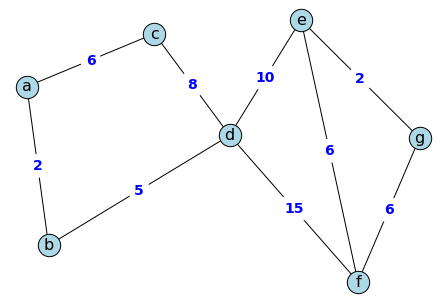
\includegraphics[scale = 0.5]{graph-theory-graphics/dijkstra0.png}\\
\end{center}
We will initialize our algorithm at node 'a'.  

\begin{minipage}{0.5\textwidth}
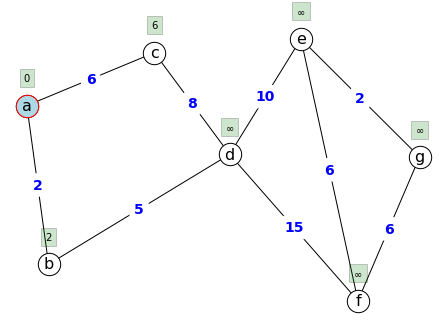
\includegraphics[scale = 0.5]{graph-theory-graphics/dijkstra1.png}
\end{minipage}
\begin{minipage}{0.5\textwidth}
         \begin{tabular}{|l|l|l|l|l|l|l|l|}
    \hline
        current & a & b & c & d & e & f & g \\ \hline
        a & 0 & 2 & 6 & $\infty$ & $\infty$ & $\infty$& $\infty$  \\ \hline
    \end{tabular} 
    \end{minipage}\\
\begin{minipage}{0.5\textwidth}
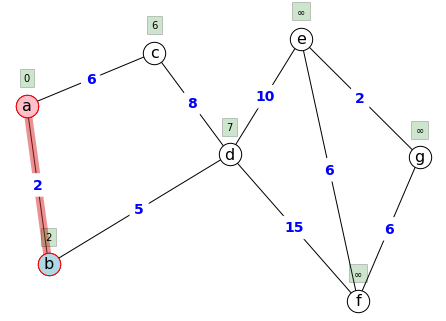
\includegraphics[scale = 0.5]{graph-theory-graphics/dijkstra2.png}
\end{minipage}
\begin{minipage}{0.5\textwidth}
         \begin{tabular}{|l|l|l|l|l|l|l|l|}
    \hline
        current & a & b & c & d & e & f & g \\ \hline
        b & 0 & 2 & 6 & 7 & $\infty$ & $\infty$ & $\infty$ \\ \hline
    \end{tabular}
     \end{minipage}\\
\begin{minipage}{0.5\textwidth}
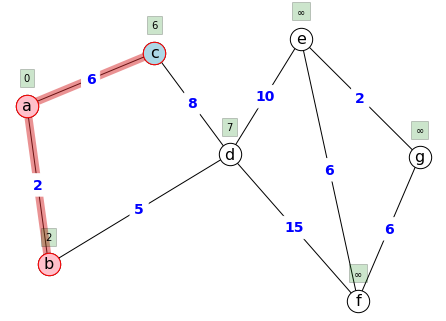
\includegraphics[scale = 0.5]{graph-theory-graphics/dijkstra3.png}
\end{minipage}
\begin{minipage}{0.5\textwidth}
          \begin{tabular}{|l|l|l|l|l|l|l|l|}
    \hline
        current & a & b & c & d & e & f & g \\ \hline
        c & 0 & 2 & 6 & 7 & $\infty$ & $\infty$ & $\infty$  \\ \hline
    \end{tabular}
     \end{minipage}\\
\begin{minipage}{0.5\textwidth}
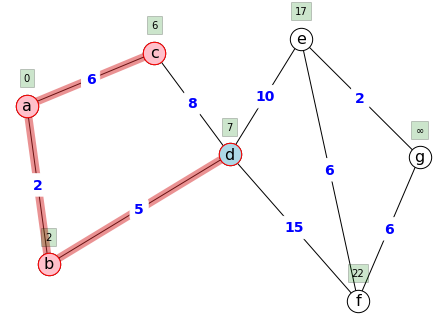
\includegraphics[scale = 0.5]{graph-theory-graphics/dijkstra4.png} 
\end{minipage}
\begin{minipage}{0.5\textwidth}
          \begin{tabular}{|l|l|l|l|l|l|l|l|}
    \hline
        current & a & b & c & d & e & f & g \\ \hline
        d & 0 & 2 & 6 & 7 & 17 & 22 & $\infty$ \\ \hline
    \end{tabular}
     \end{minipage}\\
\begin{minipage}{0.5\textwidth}
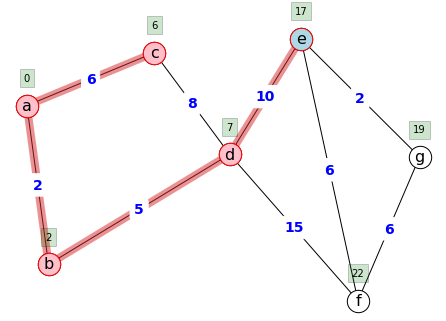
\includegraphics[scale = 0.5]{graph-theory-graphics/dijkstra5.png}
\end{minipage}
\begin{minipage}{0.5\textwidth}
         \begin{tabular}{|l|l|l|l|l|l|l|l|}
    \hline
        current & a & b & c & d & e & f & g \\ \hline
        e & 0 & 2 & 6 & 7 & 17 & 22 & 19 \\ \hline
    \end{tabular}
     \end{minipage}\\
\begin{minipage}{0.5\textwidth}
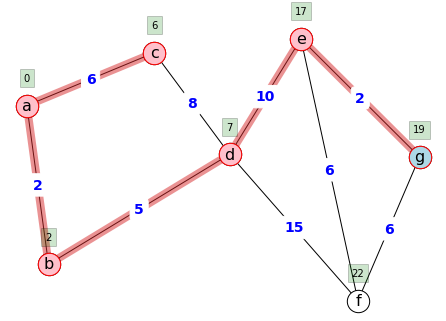
\includegraphics[scale = 0.5]{graph-theory-graphics/dijkstra6.png}
\end{minipage}
\begin{minipage}{0.5\textwidth}
          \begin{tabular}{|l|l|l|l|l|l|l|l|}
    \hline
        current & a & b & c & d & e & f & g \\ \hline
        g & 0 & 2 & 6 & 7 & 17 & 22 & 19  \\ \hline
    \end{tabular}
     \end{minipage}\\
\begin{minipage}{0.5\textwidth}
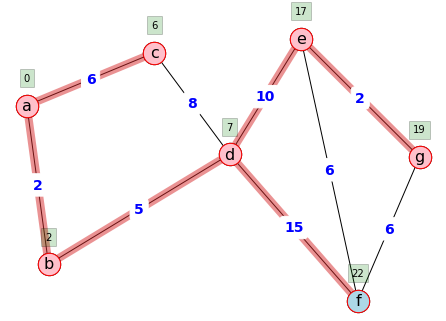
\includegraphics[scale = 0.5]{graph-theory-graphics/dijkstra7.png} 
\end{minipage}
\begin{minipage}{0.5\textwidth}
 \begin{tabular}{|l|l|l|l|l|l|l|l|}
    \hline
        current & a & b & c & d & e & f & g \\ \hline
        f & 0 & 2 & 6 & 7 & 17 & 22 & 19  \\ \hline
    \end{tabular}
\end{minipage}\\

We can now summarize our calculations that followed Dijkstra's algorithm.\\

\begin{minipage}{0.5\textwidth}
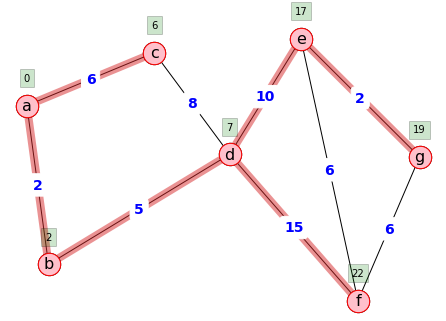
\includegraphics[scale = 0.5]{graph-theory-graphics/dijkstra8.png} 
\end{minipage}
\begin{minipage}{0.5\textwidth}
 \begin{tabular}{|l|l|l|l|l|l|l|l|}
    \hline
        current & a & b & c & d & e & f & g \\ \hline
        a & 0 & 2 & 6 & $\infty$ & $\infty$ & $\infty$& $\infty$  \\ \hline
        b & 0 & 2 & 6 & 7 & $\infty$ & $\infty$ & $\infty$ \\ \hline
        c & 0 & 2 & 6 & 7 & $\infty$ & $\infty$ & $\infty$  \\ \hline
        d & 0 & 2 & 6 & 7 & 17 & 22 & $\infty$ \\ \hline
        e & 0 & 2 & 6 & 7 & 17 & 22 & 19 \\ \hline
        g & 0 & 2 & 6 & 7 & 17 & 22 & 19  \\ \hline
        f & 0 & 2 & 6 & 7 & 17 & 22 & 19  \\ \hline
    \end{tabular}
\end{minipage}\\

\paragraph{Final solution} 
The shortest path from a to g is the path a - b - d - e - g, 
\begin{center}
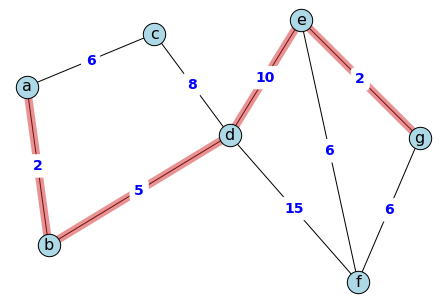
\includegraphics[scale = 0.5]{graph-theory-graphics/dijkstra-soln.png}
\end{center} 
and has length 
$$
2 + 5 + 10 + 2 = 19.
$$
\end{example}

\newpage
\newpage



\begin{example}{}{}
A shipping company needs to route a package from Washington, D.C. to San Diego, CA.  To minimize costs, the package will first be sent to their processing center in Baltimore, MD then sent as part of mass shipments between their various processing centers, ending up in their processing center in Bakersfield, CA.  From there it will be delivered in a small truck to San Diego.  

The travel times, in hours, between their processing centers are shown in the table below.  Three hours has been added to each travel time for processing.  Find the shortest path from Baltimore to Bakersfield.
 \begin{center}
 \begin{tabular}{|l|c|c|c|c|c|c|}
 \hline
 & Baltimore & Denver & Dallas & Chicago & Atlanta & Bakersfield\\
 &&&&&&\\
 \hline
 Baltimore & * &&&15&14&\\
 \hline
 Denver &&*&&18&24&19\\
 \hline
Dallas&&&*&18&15&25\\
 \hline
 Chicago &15&18&18&*&14&\\
 \hline
 Atlanta & 14 & 24&15&14&8&\\
 \hline
 Bakersfield &&19&25&&&*\\
 \hline
 \end{tabular}
 \end{center}


While we could draw a graph, we can also work directly from the table. \\

\noindent Step 1:  The ending vertex, Bakersfield, is marked as current.\\

\noindent Step 2:  All cities connected to Bakersfield, in this case Denver and Dallas, have their distances calculated; we'll mark those distances in the column headers.  \\

\noindent Step 3 \& 4:  Mark Bakersfield as visited.  Here, we are doing it by shading the corresponding row and column of the table.  We mark Denver as current, shown in bold, since it is the vertex with the shortest distance.
 \begin{center}
 \begin{tabular}{|l|c|c|c|c|c|c|}
 \hline
 & Baltimore & \textbf{Denver} & Dallas & Chicago & Atlanta & \cellcolor{yellow}Bakersfield\\
 &&[19]&[25]&&&\cellcolor{yellow}[0]\\
 \hline
 Baltimore & * &&&15&14&\cellcolor{yellow}\\
 \hline
 Denver &&*&&18&24&\cellcolor{yellow}19\\
 \hline
Dallas&&&*&18&15&\cellcolor{yellow}25\\
 \hline
 Chicago &15&18&18&*&14&\cellcolor{yellow}\\
 \hline
 Atlanta & 14 & 24&15&14&8&\cellcolor{yellow}\\
 \hline
 \cellcolor{yellow}Bakersfield &\cellcolor{yellow}&\cellcolor{yellow}19&\cellcolor{yellow}25&\cellcolor{yellow}&\cellcolor{yellow}&\cellcolor{yellow}*\\
 \hline
 \end{tabular}
 \end{center}


\noindent Step 2 (\#2):  For cities connected to Denver, calculate distance to the end.  For example, Chicago is 18 hours from Denver, and Denver is 19 hours from the end, the distance for Chicago to the end is $18+19 = 37$  (Chicago to Denver to Bakersfield).  Atlanta is 24 hours from Denver, so the distance to the end is $24+19 = 43$ (Atlanta to Denver to Bakersfield).\\

\noindent Step 3 \& 4 (\#2):  We mark Denver as visited and mark Dallas as current.
 \begin{center}
 \begin{tabular}{|l|c|c|c|c|c|c|}
 \hline
 & Baltimore & \cellcolor{yellow}Denver & \textbf{Dallas} & Chicago & Atlanta & \cellcolor{yellow}Bakersfield\\
 && \cellcolor{yellow}[19]&[25]&[37]&[43]&\cellcolor{yellow}[0]\\
 \hline
 Baltimore & * & \cellcolor{yellow}&&15&14&\cellcolor{yellow}\\
 \hline
  \cellcolor{yellow}Denver & \cellcolor{yellow}& \cellcolor{yellow}*& \cellcolor{yellow}& \cellcolor{yellow}18& \cellcolor{yellow}24&\cellcolor{yellow}19\\
 \hline
Dallas&& \cellcolor{yellow}&*&18&15&\cellcolor{yellow}25\\
 \hline
 Chicago &15& \cellcolor{yellow}18&18&*&14&\cellcolor{yellow}\\
 \hline
 Atlanta & 14 &  \cellcolor{yellow}24&15&14&8&\cellcolor{yellow}\\
 \hline
 \cellcolor{yellow}Bakersfield &\cellcolor{yellow}&\cellcolor{yellow}19&\cellcolor{yellow}25&\cellcolor{yellow}&\cellcolor{yellow}&\cellcolor{yellow}*\\
 \hline
 \end{tabular}
 \end{center}



\noindent Step 2 (\#3):  For cities connected to Dallas, calculate the distance to the end.  For Chicago, the distance from Chicago to Dallas is 18 and from Dallas to the end is 25, so the distance from Chicago to the end through Dallas would be $18+25 = 43$.  Since this is longer than the currently marked distance for Chicago, we do not replace it.  For Atlanta, we calculate $15+25 = 40$.  Since this is shorter than the currently marked distance for Atlanta, we replace the existing distance.\\

\noindent Step 3 \& 4 (\#3):  We mark Dallas as visited, and mark Chicago as current.

 \begin{center}
 \begin{tabular}{|l|c|c|c|c|c|c|}
 \hline
 & Baltimore & \cellcolor{yellow}Denver &  \cellcolor{yellow}Dallas & \textbf{Chicago} & Atlanta & \cellcolor{yellow}Bakersfield\\
 && \cellcolor{yellow}[19]& \cellcolor{yellow}[25]&[37]&[40]&\cellcolor{yellow}[0]\\
 \hline
 Baltimore & * & \cellcolor{yellow}& \cellcolor{yellow}&15&14&\cellcolor{yellow}\\
 \hline
 \cellcolor{yellow} Denver & \cellcolor{yellow}& \cellcolor{yellow}*& \cellcolor{yellow}& \cellcolor{yellow}18& \cellcolor{yellow}24&\cellcolor{yellow}19\\
 \hline
 \cellcolor{yellow}Dallas& \cellcolor{yellow}& \cellcolor{yellow}& \cellcolor{yellow}*& \cellcolor{yellow}18& \cellcolor{yellow}15&\cellcolor{yellow}25\\
 \hline
 Chicago &15& \cellcolor{yellow}18& \cellcolor{yellow}18&*&14&\cellcolor{yellow}\\
 \hline
 Atlanta & 14 &  \cellcolor{yellow}24& \cellcolor{yellow}15&14&8&\cellcolor{yellow}\\
 \hline
 \cellcolor{yellow}Bakersfield &\cellcolor{yellow}&\cellcolor{yellow}19&\cellcolor{yellow}25&\cellcolor{yellow}&\cellcolor{yellow}&\cellcolor{yellow}*\\
 \hline
 \end{tabular}
 \end{center}



\noindent Step 2 (\#4):  Baltimore and Atlanta are the only non-visited cities connected to Chicago.  For Baltimore, we calculate 15+37 = 52 and mark that distance.  For Atlanta, we calculate $14+37 = 51$.  Since this is longer than the existing distance of 40 for Atlanta, we do not replace that distance.\\


\noindent Step 3 \& 4 (\#4):  Mark Chicago as visited and Atlanta as current.

 \begin{center}
 \begin{tabular}{|l|c|c|c|c|c|c|}
 \hline
 & Baltimore & \cellcolor{yellow}Denver &  \cellcolor{yellow}Dallas &  \cellcolor{yellow}Chicago & \textbf{Atlanta} & \cellcolor{yellow}Bakersfield\\
 &[52]& \cellcolor{yellow}[19]& \cellcolor{yellow}[25]& \cellcolor{yellow}[37]&[40]&\cellcolor{yellow}[0]\\
 \hline
 Baltimore & * & \cellcolor{yellow}& \cellcolor{yellow}& \cellcolor{yellow}15&14&\cellcolor{yellow}\\
 \hline
 \cellcolor{yellow} Denver & \cellcolor{yellow}& \cellcolor{yellow}*& \cellcolor{yellow}& \cellcolor{yellow}18& \cellcolor{yellow}24&\cellcolor{yellow}19\\
 \hline
 \cellcolor{yellow}Dallas& \cellcolor{yellow}& \cellcolor{yellow}& \cellcolor{yellow}*& \cellcolor{yellow}18& \cellcolor{yellow}15&\cellcolor{yellow}25\\
 \hline
  \cellcolor{yellow}Chicago & \cellcolor{yellow}15& \cellcolor{yellow}18& \cellcolor{yellow}18& \cellcolor{yellow}*& \cellcolor{yellow}14&\cellcolor{yellow}\\
 \hline
 Atlanta & 14 &  \cellcolor{yellow}24& \cellcolor{yellow}15& \cellcolor{yellow}14&8&\cellcolor{yellow}\\
 \hline
 \cellcolor{yellow}Bakersfield &\cellcolor{yellow}&\cellcolor{yellow}19&\cellcolor{yellow}25&\cellcolor{yellow}&\cellcolor{yellow}&\cellcolor{yellow}*\\
 \hline
 \end{tabular}
 \end{center}


\noindent Step 2 (\#5):  The distance from Atlanta to Baltimore is 14.  Adding that to the distance already calculated for Atlanta gives a total distance of $14+40 = 54$ hours from Baltimore to Bakersfield through Atlanta.  Since this is larger than the currently calculated distance, we do not replace the distance for Baltimore.\\

\noindent Step 3 \& 4 (\#5):  We mark Atlanta as visited.  All cities have been visited and we are done.  

The shortest route from Baltimore to Bakersfield will take 52 hours, and will route through Chicago and Denver.
\end{example}

\begin{exercise}{}{} %2
Find the shortest path between vertices A and G in the graph below.\\

\begin{tikzpicture}
\draw[fill] (0,0) circle[radius=.1] node[left]{A};
\draw[fill] (2,2) circle[radius=.1] node[left]{B};
\draw[fill] (2,-2) circle[radius=.1] node[left]{C};
\draw[fill] (4,0) circle[radius=.1] node[left]{D};
\draw[fill] (6,2) circle[radius=.1] node[right]{E};
\draw[fill] (6,-2) circle[radius=.1] node[right]{F};
\draw[fill] (8,0) circle[radius=.1] node[right]{G};
\draw(0,0)--(2,2);
\node at (0.7,1){1};
\draw(0,0)--(2,-2);
\node at (0.7,-1){4};
\draw(2,2)--(4,0);
\node at (2.7,1){3};
\draw(2,-2)--(4,0);
\node at (2.7,-1){2};
\draw(4,0)--(6,2);
\node at (4.7,1){2};
\draw(4,0)--(6,-2);
\node at (4.7,-1){4};
\draw(6,2)--(8,0);
\node at (6.7,1){7};
\draw(6,-2)--(8,0);
\node at (6.7,-1){6};
\draw(2,2)--(6,2);
\node at (4,2.3){6};
\draw(2,-2)--(6,-2);
\node at (4,-2.3){5};
\draw(6,2)--(6,-2);
\node at (6.3,0){2};
\end{tikzpicture}
\end{exercise}



\section{Spanning Trees}
\begin{outcome}
\begin{itemize}
\item Find the smallest set of edges that connects a graph
\end{itemize}
\end{outcome}

\begin{resource}
\begin{itemize}
\item \href{https://youtu.be/d9GcoLAA-dU}{YouTube Video: Kruskal's algorithm to find a minimum weight spanning tree}
\end{itemize}
\end{resource}

A company requires reliable internet and phone connectivity between their five offices (named A, B, C, D, and E for simplicity) in New York, so they decide to lease dedicated lines from the phone company.  The phone company will charge for each link made.  The costs, in thousands of dollars per year, are shown in the graph.

\begin{center}
\begin{tikzpicture}
\draw[fill] (0,0) circle[radius=.1] node[below]{D};
\draw[fill] (3,0) circle[radius=.1] node[below]{C};
\draw[fill] (-1,1.5) circle[radius=.1] node[left]{E};
\draw[fill] (2,3) circle[radius=.1] node[above]{A};
\draw[fill] (5,1.5) circle[radius=.1] node[right]{B};
\draw(0,0)--(3,0);
\draw(0,0)--(2,3);
\draw(0,0)--(-1,1.5);
\draw(0,0)--(5,1.5);
\draw(3,0)--(-1,1.5);
\draw(3,0)--(2,3);
\draw(3,0)--(5,1.5);
\draw(-1,1.5)--(2,3);
\draw(-1,1.5)--(5,1.5);
\draw(2,3)--(5,1.5);
\node at (1.5, -0.2){\$7};
\node at (-0.9, 0.7){\$13};
\node at (4.6,0.7){\$10};
\node at (3.5, 2.5){\$4};
\node at (0.5,2.5){\$5};
\node at (1.7,1.3){\$6};
\node at (1.15,2.15){\$9};
\node at (2.5,2.15){\$8};
\node at (0,0.9){\$11};
\node at (3.4,0.85){\$14};
\end{tikzpicture}
\end{center}

In this case, we don't need to find a circuit, or even a specific path; all we need to do is make sure we can make a call from any office to any other.  In other words, we need to be sure there is a path from any vertex to any other vertex.


\begin{definition}{Spanning Tree}{}
A spanning tree is a connected graph using all vertices in which there are no circuits.  
In other words, there is a path from any vertex to any other vertex, but no circuits.   
\end{definition}

Some examples of spanning trees are shown below.  Notice there are no circuits in the trees, and it is fine to have vertices with degree higher than two.\\

\begin{minipage}{0.2\textwidth}
\begin{tikzpicture}
\draw[fill] (0,0) circle[radius=.1];
\draw[fill] (1,1) circle[radius=.1];
\draw[fill] (1,2) circle[radius=.1];
\draw[fill] (2,0) circle[radius=.1];
\draw(0,0)--(1,2);
\draw(0,0)--(1,1);
\draw(1,2)--(2,0);
\end{tikzpicture}
\end{minipage}
%
\begin{minipage}{0.2\textwidth}
\begin{tikzpicture}
\draw[fill] (0,0) circle[radius=.1];
\draw[fill] (1,1) circle[radius=.1];
\draw[fill] (1,2) circle[radius=.1];
\draw[fill] (2,0) circle[radius=.1];
\draw(0,0)--(1,2);
\draw(2,0)--(1,1);
\draw(1,2)--(2,0);
\end{tikzpicture}
\end{minipage}
%
\begin{minipage}{0.2\textwidth}
\begin{tikzpicture}
\draw[fill] (0,0) circle[radius=.1];
\draw[fill] (1,1) circle[radius=.1];
\draw[fill] (1,2) circle[radius=.1];
\draw[fill] (2,0) circle[radius=.1];
\draw(0,0)--(1,2);
\draw(0,0)--(1,1);
\draw(0,0)--(2,0);
\end{tikzpicture}
\end{minipage}
%
\begin{minipage}{0.2\textwidth}
\begin{tikzpicture}
\draw[fill] (0,0) circle[radius=.1];
\draw[fill] (1,1) circle[radius=.1];
\draw[fill] (1,2) circle[radius=.1];
\draw[fill] (2,0) circle[radius=.1];
\draw(0,0)--(1,2);
\draw(1,2)--(1,1);
\draw(1,2)--(2,0);
\end{tikzpicture}
\end{minipage}
%
\begin{minipage}{0.2\textwidth}
\begin{tikzpicture}
\draw[fill] (0,0) circle[radius=.1];
\draw[fill] (1,1) circle[radius=.1];
\draw[fill] (1,2) circle[radius=.1];
\draw[fill] (2,0) circle[radius=.1];
\draw(1,1)--(1,2);
\draw(1,2)--(2,0);
\draw(0,0)--(2,0);
\end{tikzpicture}
\end{minipage}\\

Usually we have a starting graph to work from, like in the phone example above.  In this case, we form our spanning tree by finding a \textbf{subgraph} -- a new graph formed using all the vertices but only some of the edges from the original graph.  No edges will be created where they didn't already exist.

Of course, any random spanning tree isn't really what we want.  We want the \textbf{minimum cost spanning tree (MCST)}.

\begin{definition}{Minimum Cost Spanning Tree (MCST)}{}
The minimum cost spanning tree is the spanning tree with the smallest total edge weight.  
\end{definition}


A nearest neighbor style approach doesn't make as much sense here since we don't need a circuit, so instead we will take an approach similar to sorted edges.

{\Large \textbf{Kruskal's Algorithm} } \\
%\begin{algorithm}{}{}[Kruskal's Algorithm]
\hspace{3in}
\begin{enumerate}
\item Select the cheapest unused edge in the graph.
\item Repeat step 1, adding the cheapest unused edge, unless:
\begin{itemize}
\item adding the edge would create a circuit.
\end{itemize}
\item Repeat until a spanning tree is formed.
\end{enumerate}
%\end{algorithm}



\begin{example}{}{} %22
Using our phone line graph from above, begin adding edges:\\
\begin{minipage}{.5\textwidth}
\begin{tabular}{lll}
AB&	\$4&	OK\\
AE	&\$5	&OK\\
BE	&\$6&	reject -- closes circuit ABEA\\
DC	&\$7&	OK\\
AC&\$8&	OK\\
\end{tabular}
\end{minipage}
%
\begin{minipage}{.5\textwidth}
\begin{tikzpicture}
\draw[fill] (0,0) circle[radius=.1] node[below]{D};
\draw[fill] (3,0) circle[radius=.1] node[below]{C};
\draw[fill] (-1,1.5) circle[radius=.1] node[left]{E};
\draw[fill] (2,3) circle[radius=.1] node[above]{A};
\draw[fill] (5,1.5) circle[radius=.1] node[right]{B};
\draw[very thick, red](0,0)--(3,0);
\draw(0,0)--(2,3);
\draw(0,0)--(-1,1.5);
\draw(0,0)--(5,1.5);
\draw(3,0)--(-1,1.5);
\draw[very thick, red](3,0)--(2,3);
\draw(3,0)--(5,1.5);
\draw[very thick, red](-1,1.5)--(2,3);
\draw(-1,1.5)--(5,1.5);
\draw[very thick, red](2,3)--(5,1.5);
\node at (1.5, -0.2){\$7};
\node at (-0.9, 0.7){\$13};
\node at (4.6,0.7){\$10};
\node at (3.5, 2.5){\$4};
\node at (0.5,2.5){\$5};
\node at (1.7,1.3){\$6};
\node at (1.15,2.15){\$9};
\node at (2.5,2.15){\$8};
\node at (0,0.9){\$11};
\node at (3.4,0.85){\$14};
\end{tikzpicture}
\end{minipage}

At this point we stop -- every vertex is now connected, so we have formed a spanning tree with cost \$24 thousand a year.
\end{example}

Remarkably, Kruskal's algorithm is both optimal and efficient; we are guaranteed to always produce the optimal MCST.


\begin{example}{}{} %23
The power company needs to lay updated distribution lines connecting the ten Oregon cities below to the power grid.  How can they minimize the amount of new line to lay?
 
\begin{center}
\begin{tabular}{|l|c|c|c|c|c|c|c|c|c|c|}
\hline
&&&&&&&&&&\\[7ex]
& \begin{rotate}{90}Ashland \end{rotate}& \begin{rotate}{90}Astoria\end{rotate}  & \begin{rotate}{90}Bend \end{rotate}& \begin{rotate}{90}Corvallis \end{rotate} & \begin{rotate}{90}Crater Lake \end{rotate} &  \begin{rotate}{90}Eugene  \end{rotate}&  \begin{rotate}{90}Newport \end{rotate} &  \begin{rotate}{90}Portland  \end{rotate}& \begin{rotate}{90}Salem \end{rotate} &  \begin{rotate}{90}Seaside \end{rotate}\\
\hline
Ashland & --&374&200&223&108&178&252&285&240&356\\
\hline
Astoria & 374&--&255&166&433&199&135&95&136&17\\
\hline
Bend & 200 & 255 &--&128&277&128&180 & 160&131&247\\
\hline
Corvalis&223&166&128&--&430&47&52&84&40&155\\
\hline
Crater Lake &108&433&277&430&--&453&478&344&389&423\\
\hline
Eugene &178&199&128&47&453&--&91&110&64&181\\
\hline
Newport&252&135&180&52&478&91&--&114&83&117\\
\hline
Portland &285&95&160&84&344&110&114&--&47&78\\
\hline
Salem & 240 &136&131&40&389&64&83&47&--&118\\
\hline
Seaside&356&17&247&155&423&181&117&78&118&--\\
\hline
\end{tabular}
\end{center}

Using Kruskal's algorithm, we add edges from cheapest to most expensive, rejecting any that close a circuit.  We stop when the graph is connected.\\

\begin{minipage}{0.5\textwidth}
\begin{tabular}{ll}
Seaside to Astoria&		17 miles\\
Corvallis to Salem	&	40 miles\\
Portland to Salem	&	47 miles\\
Corvallis to Eugene	&	47 miles\\
Corvallis to Newport	&	52 miles\\
Salem to Eugene	&	reject -- closes circuit\\
Portland to Seaside	&	78 miles\\
\end{tabular}\\

The graph up to this point is shown to the right.
\end{minipage}
%
\begin{minipage}{0.5\textwidth}
\scalebox{0.7}{
\begin{tikzpicture}
\draw[fill] (2,-2) circle[radius=.1] node[below]{Portland};
\draw[fill] (1,0) circle[radius=.1] node[above]{Salem};
\draw[fill] (9,0) circle[radius=.1] node[above]{Corvalis};
\draw[fill] (2,2) circle[radius=.1] node[above]{Seaside};
\draw[fill] (4,3) circle[radius=.1] node[above]{Ashland};
\draw[fill] (4,-3) circle[radius=.1] node[below]{Newport};
\draw[fill] (6,3) circle[radius=.1] node[above]{Astoria};
\draw[fill] (6,-3) circle[radius=.1] node[below]{Eugene};
\draw[fill] (8,2) circle[radius=.1] node[above]{Bend};
\draw[fill] (8,-2) circle[radius=.1] node[below]{Crater Lake};
\draw(1,0)--(9,0);
\draw(1,0)--(2,-2);
\draw(2,2)--(6,3);
\draw(9,0)--(4,-3);
\draw(9,0)--(6,-3);
\draw(2,2)--(2,-2);
\end{tikzpicture}
}
\end{minipage}

Continuing,

\begin{minipage}{0.5\textwidth}
\begin{tabular}{ll}
Newport to Salem&		reject \\
Corvallis to Portland&		reject\\ 
Eugene to Newport	&	reject\\
Portland to Astoria	&	reject\\
Ashland to Crater Lake	&	108 miles\\
Eugene to Portland	&	reject \\
Newport to Portland	&	reject\\
Newport to Seaside	&	reject \\
Salem to Seaside	&	reject\\
Bend to Eugene	&	128 miles\\
Bend to Salem		&	reject \\
Astoria to Newport 	&	reject \\
Salem to Astoria 	&	reject \\
Corvallis to Seaside	&	reject \\
Portland to Bend	&	reject \\
Astoria to Corvallis	&	reject \\
Eugene to Ashland	&	178 miles\\
\end{tabular}\\

This connects the graph.  The total length of cable to lay would be 695 miles.
\end{minipage}
%
\begin{minipage}{0.5\textwidth}
\vspace{1in}
\scalebox{0.7}{
\begin{tikzpicture}
\draw[fill] (2,-2) circle[radius=.1] node[below]{Portland};
\draw[fill] (1,0) circle[radius=.1] node[above]{Salem};
\draw[fill] (9,0) circle[radius=.1] node[above]{Corvalis};
\draw[fill] (2,2) circle[radius=.1] node[above]{Seaside};
\draw[fill] (4,3) circle[radius=.1] node[above]{Ashland};
\draw[fill] (4,-3) circle[radius=.1] node[below]{Newport};
\draw[fill] (6,3) circle[radius=.1] node[above]{Astoria};
\draw[fill] (6,-3) circle[radius=.1] node[below]{Eugene};
\draw[fill] (8,2) circle[radius=.1] node[above]{Bend};
\draw[fill] (8,-2) circle[radius=.1] node[below]{Crater Lake};
\draw(1,0)--(9,0);
\draw(1,0)--(2,-2);
\draw(2,2)--(6,3);
\draw(9,0)--(4,-3);
\draw(9,0)--(6,-3);
\draw(8,-2)--(4,3);
\draw(4,3)--(6,-3);
\draw(6,-3)--(8,2);
\draw(2,2)--(2,-2);
\end{tikzpicture}
}
\end{minipage}

\end{example}



\begin{exercise}{Min Cost Spanning Tree}{kruskal_exercise} %7
Find a minimum cost spanning tree on the graph below using Kruskal's algorithm.\\
\begin{tikzpicture}
\draw[fill] (0,0) circle[radius=.1] node[left]{A};
\draw[fill] (2,2) circle[radius=.1] node[above]{B};
\draw[fill] (2,-2) circle[radius=.1] node[below]{C};
\draw[fill] (4,2) circle[radius=.1] node[above]{E};
\draw[fill] (4,-2) circle[radius=.1] node[below]{F};
\draw[fill] (6,0) circle[radius=.1] node[right]{G};
\draw(0,0) to node[above]{11} (2,2);
\draw(0,0) to node[below]{33}(2,-2);
\draw(0,0) to node[pos=0.3, fill=ocre!10]{14}(4,2);
\draw(0,0) to node[pos=0.3, fill=ocre!10]{41}(4,-2);
\draw(0,0) to node[near start, fill=ocre!10]{15}(6,0);
\draw(2,2) to node[pos=0.37, fill=ocre!10]{25}(2,-2);
\draw(2,2) to node[above]{43}(4,2);
\draw(2,2) to node[pos=0.7, fill=ocre!10]{23}(4,-2);
\draw(2,2) to node[pos=0.7, fill=ocre!10]{13}(6,0);
\draw(2,-2) to node[pos=0.35, fill=ocre!10]{17} (4,2);
\draw(2,-2) to node[below]{37}(4,-2);
\draw(2,-2) to node[pos=0.7, fill=ocre!10]{36}(6,0);
\draw(4,2) to node[pos=0.38, fill=ocre!10]{16}(4,-2);
\draw(4,2) to node[above]{45}(6,0);
\draw(4,-2) to node[below]{19}(6,0);
\end{tikzpicture}
\end{exercise}





\section{Exercise Answers}
\begin{enumerate}
\item  \begin{enumerate}
\item 5 vertices, 10 edges
\item Yes, it is connected.
\item The vertex is degree 4.
\item A path
\item  A circuit\\
\end{enumerate}

\item The shortest path is ABDEG, with length 13.\\

\item Yes, all vertices have even degree so this graph has an Euler Circuit.  There are several possibilities.  One is:  ABEGFCDFEDBCA\\


\item \hspace{.2in}\\
\begin{minipage}{0.5\textwidth}
This graph can be eulerized by duplicating the edge BC, as shown.  One possible Euler circuit on the eulerized graph is ACDBCBA.
\end{minipage}
%
\begin{minipage}{0.5\textwidth}
\scalebox{.7}{
\begin{tikzpicture}
\draw[fill] (0,0) circle[radius=.1] node [left]{B};
\draw[fill] (4,0) circle[radius=.1] node [right]{C};
\draw[fill] (2,2) circle[radius=.1] node [above]{D};
\draw[fill] (2,4) circle[radius=.1] node [above]{A};
\draw(0,0)--(4,0);
\draw(0,0)--(2,2);
\draw(0,0)--(2,4);
\draw(4,0)--(2,2);
\draw(4,0)--(2,4);
\draw[very thick, red](0,0) to [bend right] (4,0);
\end{tikzpicture}
}
\end{minipage}

\item At each step, we look for the nearest location we haven't already visited.  \\
From B the nearest computer is E with time 24.  \\
From E, the nearest computer is D with time 11.  \\
From D the nearest is A with time 12. \\
From A the nearest is C with time 34.  \\
From C, the only computer we haven't visited is F with time 27.\\
From F, we return back to B with time 50.\\

\noindent The NNA circuit from B is BEDACFB with time 158 milliseconds.\\

\noindent Using NNA again from other starting vertices:\\
Starting at A: ADEBCFA: time 146\\
Starting at C: CDEBAFC: time 167\\
Starting at D: DEBCFAD: time 146\\
Starting at E: EDACFBE: time 158\\
Starting at F: FDEBCAF: time 158\\

\noindent The RNNA found a circuit with time 146 milliseconds:  ADEBCFA.  We could also write this same circuit starting at B if we wanted:  BCFADEB or BEDAFCB.\\

\item \hspace{.2in}\\
\begin{minipage}{0.5\textwidth}
AB: Add, cost 11\\
BG: Add, cost 13\\
AE: Add, cost 14\\
EF: Add, cost 15\\
EC: Skip (degree 3 at E)\\
FG: Skip (would create a circuit not including C)\\
BF, BC, AG, AC: Skip (would cause a vertex to have degree 3)\\
GC: Add, cost 36\\
CF: Add, cost 37, completes the circuit\\

\noindent Final circuit:  ABGCFEA\\
\end{minipage}
%
\begin{minipage}{0.5\textwidth}
\begin{tikzpicture}
\draw[fill] (0,0) circle[radius=.1] node[left]{A};
\draw[fill] (2,2) circle[radius=.1] node[above]{B};
\draw[fill] (2,-2) circle[radius=.1] node[below]{C};
\draw[fill] (4,2) circle[radius=.1] node[above]{E};
\draw[fill] (4,-2) circle[radius=.1] node[below]{F};
\draw[fill] (6,0) circle[radius=.1] node[right]{G};
\draw[very thick, red](0,0) to node[above]{11} (2,2);
\draw(0,0) to node[below]{33}(2,-2);
\draw[very thick, red](0,0) to node[pos=0.3, fill=white]{14}(4,2);
\draw(0,0) to node[pos=0.3, fill=white]{41}(4,-2);
\draw(0,0) to node[near start, fill=white]{27}(6,0);
\draw(2,2) to node[pos=0.37, fill=white]{25}(2,-2);
\draw(2,2) to node[above]{43}(4,2);
\draw(2,2) to node[pos=0.7, fill=white]{23}(4,-2);
\draw[very thick, red](2,2) to node[pos=0.7, fill=white]{13}(6,0);
\draw(2,-2) to node[pos=0.35, fill=white]{17} (4,2);
\draw[very thick, red](2,-2) to node[below]{37}(4,-2);
\draw[very thick, red](2,-2) to node[pos=0.7, fill=white]{36}(6,0);
\draw[very thick, red](4,2) to node[pos=0.38, fill=white]{15}(4,-2);
\draw(4,2) to node[above]{45}(6,0);
\draw(4,-2) to node[below]{19}(6,0);
\end{tikzpicture}
\end{minipage}

\item (\ref{exa:kruskal_exercise})\hspace{.2in}\\
\begin{minipage}{0.5\textwidth}
AB: Add, cost 11\\
BG: Add, cost 13\\
AE: Add, cost 14\\
AG: Skip, would create circuit ABGA\\
EF: Add, cost 16\\
EC: Add, cost 17\\

\noindent This completes the spanning tree.\\
\end{minipage}
%
\begin{minipage}{0.5\textwidth}
\begin{tikzpicture}
\draw[fill] (0,0) circle[radius=.1] node[left]{A};
\draw[fill] (2,2) circle[radius=.1] node[above]{B};
\draw[fill] (2,-2) circle[radius=.1] node[below]{C};
\draw[fill] (4,2) circle[radius=.1] node[above]{E};
\draw[fill] (4,-2) circle[radius=.1] node[below]{F};
\draw[fill] (6,0) circle[radius=.1] node[right]{G};
\draw[very thick, red](0,0) to node[above]{11} (2,2);
\draw(0,0) to node[below]{33}(2,-2);
\draw[very thick, red](0,0) to node[pos=0.3, fill=white]{14}(4,2);
\draw(0,0) to node[pos=0.3, fill=white]{41}(4,-2);
\draw(0,0) to node[near start, fill=white]{15}(6,0);
\draw(2,2) to node[pos=0.37, fill=white]{25}(2,-2);
\draw(2,2) to node[above]{43}(4,2);
\draw(2,2) to node[pos=0.7, fill=white]{23}(4,-2);
\draw[very thick, red](2,2) to node[pos=0.7, fill=white]{13}(6,0);
\draw[very thick, red](2,-2) to node[pos=0.35, fill=white]{17} (4,2);
\draw(2,-2) to node[below]{37}(4,-2);
\draw(2,-2) to node[pos=0.7, fill=white]{36}(6,0);
\draw[very thick, red](4,2) to node[pos=0.38, fill=white]{16}(4,-2);
\draw(4,2) to node[above]{45}(6,0);
\draw(4,-2) to node[below]{19}(6,0);
\end{tikzpicture}

\end{minipage}
\end{enumerate}
\section{Additional Exercises}

\textbf{Skills}
\begin{enumerate}
\item	To deliver mail in a particular neighborhood, the postal carrier needs to walk along each of the streets with houses (the dots).  Create a graph with edges showing where the carrier must walk to deliver the mail.\\

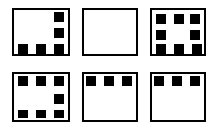
\includegraphics{graph-theory-graphics/GraphExercise1.png}\\

\item	Suppose that a town has 7 bridges as pictured below.  Create a graph that could be used to determine if there is a path that crosses all bridges once.\\

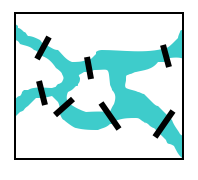
\includegraphics{graph-theory-graphics/GraphExercise2.png}\\

\item	The table below shows approximate driving times (in minutes, without traffic) between five cities in the Dallas area.  Create a weighted graph representing this data.
\begin{center}
\begin{tabular}{|l|c|c|c|c|}
\hline
&Plano&Mesquite&Arlington&Denton\\
\hline
Fort Worth&54&52&19&42\\
\hline
Plano&&38&53&41\\
\hline
Mesquite&&&43&56\\
\hline
Arlington&&&&50\\
\hline
\end{tabular}
\end{center}

\item	Shown in the table below are the one-way airfares between 5 cities\footnote{Cheapest fares found when retrieved Sept. 1, 2009 for travel Sept. 22, 2009}.  Create a graph showing this data.
\begin{center}
\begin{tabular}{|l|c|c|c|c|}
\hline
&Honolulu&London&Moscow&Cairo\\
\hline
Seattle &\$159 &\$370&\$654&\$684\\
\hline
Honolulu&&\$830&\$854&\$801\\
\hline
London&&&\$245&\$323\\
\hline
Moscow&&&&\$329\\
\hline
\end{tabular}
\end{center}

\item	Find the degree of each vertex in the graph below.\\

\begin{tikzpicture}
\draw[fill] (0,0) circle[radius=.1];
\draw[fill] (1,0) circle[radius=.1];
\draw[fill] (0,1) circle[radius=.1];
\draw[fill] (1,1) circle[radius=.1];
\draw[fill] (2,1) circle[radius=.1];
\draw(0,0)--(1,0);
\draw(1,0)--(1,1);
\draw(1,0)--(0,1);
\draw(1,1)--(0,1);
\draw(1,1)--(2,1);
\draw(2,1)--(1,0);
\end{tikzpicture}

\item	Find the degree of each vertex in the graph below.\\

\begin{tikzpicture}
\draw[fill] (0,0) circle[radius=.1];
\draw[fill] (-1,1) circle[radius=.1];
\draw[fill] (-.5,2) circle[radius=.1];
\draw[fill] (1,1) circle[radius=.1];
\draw[fill] (.5,2) circle[radius=.1];
\draw(0,0)--(-1,1);
\draw(0,0)--(1,1);
\draw(-1,1)--(1,1);
\draw(-1,1)--(-0.5,2);
\draw(1,1)--(0.5,2);
\end{tikzpicture}

\item	Which of these graphs are connected?\\

\begin{tabular}{|c|c|c|}
\hline
&&\\
\begin{tikzpicture}
\draw[fill] (0,0) circle[radius=.1];
\draw[fill] (1,0) circle[radius=.1];
\draw[fill] (0,1) circle[radius=.1];
\draw[fill] (1,1) circle[radius=.1];
\draw[fill] (2,1) circle[radius=.1];
\draw(0,0)--(1,0);
\draw(1,0)--(1,1);
\draw(0,1)--(1,1);
\draw(1,0)--(2,1);
\end{tikzpicture}
&
\begin{tikzpicture}
\draw[fill] (0,0) circle[radius=.1];
\draw[fill] (1,0) circle[radius=.1];
\draw[fill] (0,1) circle[radius=.1];
\draw[fill] (1,1) circle[radius=.1];
\draw[fill] (2,1) circle[radius=.1];
\draw(1,0)--(1,1);
\draw(1,0)--(2,1);
\draw(1,1)--(2,1);
\draw(0,0)--(0,1);
\end{tikzpicture}
&
\begin{tikzpicture}
\draw[fill] (0,0) circle[radius=.1];
\draw[fill] (1,0) circle[radius=.1];
\draw[fill] (0,1) circle[radius=.1];
\draw[fill] (1,1) circle[radius=.1];
\draw[fill] (2,1) circle[radius=.1];
\draw(0,0)--(1,0);
\draw(1,0)--(1,1);
\draw(0,1)--(1,1);
\draw(1,0)--(2,1);
\draw(1,1)--(2,1);
\draw(0,0)--(0,1);
\end{tikzpicture}\\
&&\\
\hline
\end{tabular}\\


\item Which of these graphs are connected?\\

\begin{tabular}{|c|c|c|}
\hline
&&\\
\begin{tikzpicture}
\draw[fill] (0,0) circle[radius=.1];
\draw[fill] (1,0) circle[radius=.1];
\draw[fill] (2,0) circle[radius=.1];
\draw[fill] (.5,1) circle[radius=.1];
\draw[fill] (1.5,1) circle[radius=.1];
\draw[fill] (0,2) circle[radius=.1];
\draw[fill] (1,2) circle[radius=.1];
\draw[fill] (2,2) circle[radius=.1];
\draw(0,0)--(1,0);
\draw(1,0)--(2,0);
\draw(0.5,1)--(1.5,1);
\draw(0,2)--(1,2);
\draw(1,2)--(2,2);
\end{tikzpicture}
&
\begin{tikzpicture}
\draw[fill] (0,0) circle[radius=.1];
\draw[fill] (1,0) circle[radius=.1];
\draw[fill] (2,0) circle[radius=.1];
\draw[fill] (.5,1) circle[radius=.1];
\draw[fill] (1.5,1) circle[radius=.1];
\draw[fill] (0,2) circle[radius=.1];
\draw[fill] (1,2) circle[radius=.1];
\draw[fill] (2,2) circle[radius=.1];
\draw(0,0)--(1,0);
\draw(1,0)--(1.5,1);
\draw(0.5,1)--(1.5,1);
\draw(0,2)--(0.5,1);
\draw(1,2)--(2,2);
\draw(1.5,1)--(2,2);
\draw(1.5,1)--(2,0);
\end{tikzpicture}
&
\begin{tikzpicture}
\draw[fill] (0,0) circle[radius=.1];
\draw[fill] (1,0) circle[radius=.1];
\draw[fill] (2,0) circle[radius=.1];
\draw[fill] (.5,1) circle[radius=.1];
\draw[fill] (1.5,1) circle[radius=.1];
\draw[fill] (0,2) circle[radius=.1];
\draw[fill] (1,2) circle[radius=.1];
\draw[fill] (2,2) circle[radius=.1];
\draw(0,0)--(1,0);
\draw(1,0)--(1.5,1);
\draw(0.5,1)--(1.5,1);
\draw(0,2)--(0,0);
\draw(1,2)--(2,2);
\draw(2,2)--(2,0);
\draw(0,2)--(.5,1);
\end{tikzpicture}\\
&&\\
\hline
\end{tabular}\\

\item	Travel times by rail for a segment of the Eurail system is shown below with travel times in hours and minutes.  Find path with shortest travel time from Bern to Berlin by applying Dijkstra's algorithm.\\

\begin{tikzpicture}
\draw[fill] (0,0) circle[radius=.1] node[left]{Paris};
\draw[fill] (2,-3) circle[radius=.1] node[left]{Lyon};
\draw[fill] (4,-2.5) circle[radius=.1] node[below]{Bern};
\draw[fill] (6,-1.5) circle[radius=.1] node[left]{Frankfurt};
\draw[fill] (8,-2) circle[radius=.1] node[below]{M\"unchen};
\draw[fill] (4.5,2) circle[radius=.1] node[above]{Amsterdam};
\draw[fill] (7,2) circle[radius=.1] node[above]{Berlin};
\draw(0,0) to node[above]{1:25} (4.5,2);
\draw(0,0) to node[left]{1:55} (2,-3);
\draw(2,-3) to node[below]{3:50} (4,-2.5);
\draw(4,-2.5) to node[left]{3.55} (6,-1.5);
\draw(6,-1.5) to node[above]{3:10} (8,-2);
\draw(6,-1.5) to node[left]{4:00} (4.5,2);
\draw(8,-2) to node[right]{5:45} (7,2);
\draw(7,2) to node[below]{6:10} (4.5,2);
\end{tikzpicture}


\item	Using the graph from the previous problem, find the path with shortest travel time from Paris to M\"unchen.

\item	Does each of these graphs have an Euler circuit?  If so, find it.\\

\begin{tabular}{|c|c|c|}
\hline
&&\\
\begin{tikzpicture}
\draw[fill] (0,0) circle[radius=.1];
\draw[fill] (1,1) circle[radius=.1];
\draw[fill] (2,0) circle[radius=.1];
\draw[fill] (0,2) circle[radius=.1];
\draw[fill] (2,2) circle[radius=.1];
\draw(0,0)--(2,0);
\draw(0,0)--(1,1);
\draw(1,1)--(0,2);
\draw(0,2)--(2,2);
\draw(1,1)--(2,2);
\draw(1,1)--(2,0);
\end{tikzpicture}
&
\begin{tikzpicture}
\draw[fill] (0,0) circle[radius=.1];
\draw[fill] (1,1) circle[radius=.1];
\draw[fill] (1,0) circle[radius=.1];
\draw[fill] (2,0) circle[radius=.1];
\draw[fill] (1,-1) circle[radius=.1];
\draw[fill] (2,-1) circle[radius=.1];
\draw(0,0)--(1,0);
\draw(1,0)--(2,0);
\draw(0,0)--(1,1);
\draw(1,1)--(1,0);
\draw(1,0)--(1,-1);
\draw(1,1)--(2,0);
\draw(1,-1)--(2,0);
\draw(2,0)--(2,-1);
\draw(2,-1)--(1,-1);
\draw(0,0)--(1,-1);
\end{tikzpicture}
&
\begin{tikzpicture}
\draw[fill] (0,0) circle[radius=.1];
\draw[fill] (1,1) circle[radius=.1];
\draw[fill] (2,0) circle[radius=.1];
\draw[fill] (0,2) circle[radius=.1];
\draw[fill] (2,2) circle[radius=.1];
\draw(0,0) to [bend right](1,1);
\draw(0,0) to [bend left](1,1);
\draw(1,1)--(0,2);
\draw(0,0)--(2,0);
\draw(1,1)--(2,2);
\draw(0,2)--(2,2);
\draw(2,0)--(2,2);
\draw(0,0)--(0,2);
\draw(1,1)--(2,0);
\end{tikzpicture}\\
&&\\
\hline
\end{tabular}\\


\item	Does each of these graphs have an Euler circuit?  If so, find it.\\

\begin{tabular}{|c|c|c|}
\hline
&&\\
\begin{tikzpicture}
\draw[fill] (0,0) circle[radius=.1];
\draw[fill] (2,1) circle[radius=.1];
\draw[fill] (4,0) circle[radius=.1];
\draw[fill] (1,-2) circle[radius=.1];
\draw[fill] (3,-2) circle[radius=.1];
\draw(0,0)--(2,1)--(4,0)--(3,-2)--(1,-2)--(0,0)--(4,0)--(1,-2)--(2,1)--(3,-2)--(0,0);
\end{tikzpicture}
&
\begin{tikzpicture}
\draw[fill] (0,0) circle[radius=.1];
\draw[fill] (2,0) circle[radius=.1];
\draw[fill] (4,0) circle[radius=.1];
\draw[fill] (1,1) circle[radius=.1];
\draw[fill] (3,1) circle[radius=.1];
\draw[fill] (2,2) circle[radius=.1];
\draw(0,0)--(2,0)--(4,0)--(3,1)--(2,0)--(1,1)--(0,0);
\draw(1,1)--(3,1)--(2,2)--(1,1);

\end{tikzpicture}
&
\begin{tikzpicture}
\draw[fill] (0,0) circle[radius=.1];
\draw[fill] (3,0) circle[radius=.1];
\draw[fill] (0,2) circle[radius=.1];
\draw[fill] (3,2) circle[radius=.1];
\draw[fill] (1.5,1) circle[radius=.1];
\draw(0,0)--(3,0)--(3,2)--(0,2)--(0,0);
\draw(0,2)--(1.5,1)--(3,2);

\end{tikzpicture}\\
&&\\
\hline
\end{tabular}\\


\item	Eulerize this graph using as few edge duplications as possible.  Then, find an Euler circuit.\\

\begin{tikzpicture}
\draw[fill] (0,0) circle[radius=.1];
\draw[fill] (1,0) circle[radius=.1];
\draw[fill] (2,0) circle[radius=.1];
\draw[fill] (0,1) circle[radius=.1];
\draw[fill] (1,1) circle[radius=.1];
\draw[fill] (2,1) circle[radius=.1];
\draw[fill] (0,2) circle[radius=.1];
\draw[fill] (1,2) circle[radius=.1];
\draw[fill] (2,2) circle[radius=.1];
\draw[fill] (0,3) circle[radius=.1];
\draw[fill] (1,3) circle[radius=.1];
\draw[fill] (2,3) circle[radius=.1];
\draw(0,0)--(1,0)--(2,0)--(2,1)--(1,1)--(0,1)--(0,2)--(1,2)--(2,2)--(2,3)--(1,3)--(0,3)--(0,2);
\draw(1,3)--(1,2)--(1,1)--(1,0);
\draw(0,0)--(0,1);
\draw(2,1)--(2,2);
\end{tikzpicture}

\item	Eulerize this graph using as few edge duplications as possible.  Then, find an Euler circuit.\\

\begin{tikzpicture}
\draw[fill] (0,0) circle[radius=.1];
\draw[fill] (2,0) circle[radius=.1];
\draw[fill] (4,0) circle[radius=.1];
\draw[fill] (6,0) circle[radius=.1];
\draw[fill] (0,1) circle[radius=.1];
\draw[fill] (2,1) circle[radius=.1];
\draw[fill] (4,1) circle[radius=.1];
\draw[fill] (6,1) circle[radius=.1];
\draw[fill] (0,2) circle[radius=.1];
\draw[fill] (2,2) circle[radius=.1];
\draw[fill] (4,2) circle[radius=.1];
\draw[fill] (6,2) circle[radius=.1];
\draw[fill] (0,3) circle[radius=.1];
\draw[fill] (2,3) circle[radius=.1];
\draw[fill] (4,3) circle[radius=.1];
\draw[fill] (6,3) circle[radius=.1];
\draw(0,0)--(2,0)--(4,0)--(6,0)--(6,1)--(6,2)--(6,3)--(4,3)--(2,3)--(0,3)--(0,2)--(2,2)--(2,1)--(0,1)--(0,0);
\draw(2,0)--(2,1)--(4,1)--(6,1);
\draw(2,2)--(2,3);
\draw(4,3)--(4,2)--(4,1);
\draw(4,2)--(6,2);
\end{tikzpicture}



\item	The maintenance staff at an amusement park need to patrol the major walkways, shown in the graph below, collecting litter.  Find an efficient patrol route by finding an Euler circuit.  If necessary, eulerize the graph in an efficient way.\\

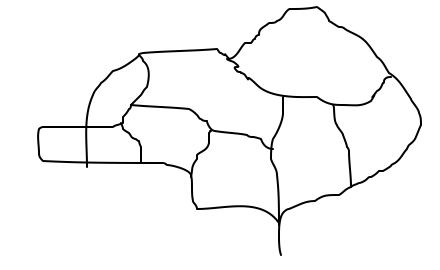
\includegraphics{graph-theory-graphics/GraphExercise15.png}\\

\item	After a storm, the city crew inspects for trees or brush blocking the road.  Find an efficient route for the neighborhood below by finding an Euler circuit.  If necessary, eulerize the graph in an efficient way.\\

\begin{tikzpicture}
\draw[fill] (1,0) circle[radius=.1];
\draw[fill] (2,0) circle[radius=.1];
\draw[fill] (3,0) circle[radius=.1];
\draw[fill] (4,0) circle[radius=.1];
\draw[fill] (5,0) circle[radius=.1];
\draw[fill] (6,0) circle[radius=.1];
\draw[fill] (0,1) circle[radius=.1];
\draw[fill] (1,1) circle[radius=.1];
\draw[fill] (4,1) circle[radius=.1];
\draw[fill] (5,1) circle[radius=.1];
\draw[fill] (0,2) circle[radius=.1];
\draw[fill] (1,2) circle[radius=.1];
\draw[fill] (2,2) circle[radius=.1];
\draw[fill] (3,2) circle[radius=.1];
\draw[fill] (0,3) circle[radius=.1];
\draw[fill] (1,3) circle[radius=.1];
\draw[fill] (2,3) circle[radius=.1];
\draw[fill] (3,3) circle[radius=.1];
\draw(1,0)--(2,0)--(3,0)--(4,0)--(5,0)--(6,0)--(5,1)--(4,1)--(5,0);
\draw(4,1)--(3,2)--(2,2)--(2,0);
\draw(1,0)--(1,1)--(0,1)--(0,2)--(0,3)--(1,3)--(2,3)--(3,3)--(3,2);
\draw (1,3)--(1,2)--(1,1);
\draw(1,2)--(2,2);
\end{tikzpicture}

\item	Does each of these graphs have at least one Hamiltonian circuit?  If so, find one. \\

\begin{tabular}{|c|c|c|}
\hline
&&\\
\begin{tikzpicture}
\draw[fill] (0,0) circle[radius=.1];
\draw[fill] (1,1) circle[radius=.1];
\draw[fill] (2,0) circle[radius=.1];
\draw[fill] (0,2) circle[radius=.1];
\draw[fill] (2,2) circle[radius=.1];
\draw(0,0)--(2,0);
\draw(0,0)--(1,1);
\draw(1,1)--(0,2);
\draw(0,2)--(2,2);
\draw(1,1)--(2,2);
\draw(1,1)--(2,0);
\end{tikzpicture}
&
\begin{tikzpicture}
\draw[fill] (0,0) circle[radius=.1];
\draw[fill] (1.5,0) circle[radius=.1];
\draw[fill] (3,0) circle[radius=.1];
\draw[fill] (0,2) circle[radius=.1];
\draw[fill] (1.5,2) circle[radius=.1];
\draw[fill] (3,2) circle[radius=.1];
\draw(0,0)--(0,2);
\draw(0,0)--(1.5,2);
\draw(0,0)--(3,2);
\draw(1.5,0)--(0,2);
\draw(1.5,0)--(1.5,2);
\draw(1.5,0)--(3,2);
\draw(3,0)--(0,2);
\draw(3,0)--(1.5,2);
\draw(3,0)--(3,2);
\end{tikzpicture}
&
\begin{tikzpicture}
\draw[fill] (0,0) circle[radius=.1];
\draw[fill] (1,0) circle[radius=.1];
\draw[fill] (2,0) circle[radius=.1];
\draw[fill] (0,1) circle[radius=.1];
\draw[fill] (1,1) circle[radius=.1];
\draw[fill] (2,1) circle[radius=.1];
\draw[fill] (1,2) circle[radius=.1];
\draw(0,0)--(1,0)--(2,0)--(2,1)--(1,2)--(0,1)--(0,0);
\draw(0,1)--(1,0)--(2,1)--(1,1)--(0,1);
\end{tikzpicture}\\
&&\\
\hline
\end{tabular}\\

\item	Does each of these graphs have at least one Hamiltonian circuit?  If so, find one. \\

\begin{tabular}{|c|c|c|}
\hline
&&\\
\begin{tikzpicture}
\draw[fill] (0,0) circle[radius=.1];
\draw[fill] (2,0) circle[radius=.1];
\draw[fill] (0,2) circle[radius=.1];
\draw[fill] (2,2) circle[radius=.1];
\draw[fill] (.7,.7) circle[radius=.1];
\draw[fill] (1.4,.7) circle[radius=.1];
\draw[fill] (.7,1.4) circle[radius=.1];
\draw[fill] (1.4,1.4) circle[radius=.1];
\draw(0,0)--(2,0)--(2,2)--(0,2)--(0,0);
\draw(.7,.7)--(1.4,.7)--(1.4,1.4)--(.7,1.4)--(.7,.7);
\draw(0,0)--(.7,.7);
\draw(2,0)--(1.4,.7);
\draw(2,2)--(1.4,1.4);
\draw(0,2)--(.7,1.4);
\end{tikzpicture}
&
\begin{tikzpicture}
\draw[fill] (0,0) circle[radius=.1];
\draw[fill] (1.5,0) circle[radius=.1];
\draw[fill] (3,0) circle[radius=.1];
\draw[fill] (0.75,2) circle[radius=.1];
\draw[fill] (2.25,2) circle[radius=.1];
\draw(0,0)--(0.75,2);
\draw(0,0)--(2.25,2);
\draw(1.5,0)--(0.75,2);
\draw(1.5,0)--(2.25,2);
\draw(3,0)--(0.75,2);
\draw(3,0)--(2.25,2);
\end{tikzpicture}
&
\begin{tikzpicture}
\draw[fill] (0,0) circle[radius=.1];
\draw[fill] (1,1) circle[radius=.1];
\draw[fill] (1,0) circle[radius=.1];
\draw[fill] (2,0) circle[radius=.1];
\draw[fill] (1,-1) circle[radius=.1];
\draw[fill] (2,-1) circle[radius=.1];
\draw(0,0)--(1,0);
\draw(1,0)--(2,0);
\draw(0,0)--(1,1);
\draw(1,1)--(1,0);
\draw(1,0)--(1,-1);
\draw(1,1)--(2,0);
\draw(1,-1)--(2,0);
\draw(2,0)--(2,-1);
\draw(2,-1)--(1,-1);
\draw(0,0)--(1,-1);
\end{tikzpicture}
\\
\hline
\end{tabular}\\

\item	A company needs to deliver product to each of their 5 stores around the Dallas, TX area.  Driving distances between the stores are shown below.  Find a route for the driver to follow, returning to the distribution center in Fort Worth:
\begin{enumerate}
\item	Using Nearest Neighbor starting in Fort Worth
\item	Using Repeated Nearest Neighbor
\item	Using Sorted Edges
\end{enumerate}
\begin{center}
\begin{tabular}{|l|c|c|c|c|}
\hline
&Plano&Mesquite&Arlington&Denton\\
\hline
Fort Worth&54&52&19&42\\
\hline
Plano&&38&53&41\\
\hline
Mesquite&&&43&56\\
\hline
Arlington&&&&50\\
\hline
\end{tabular}
\end{center}

\item	A salesperson needs to travel from Seattle to Honolulu, London, Moscow, and Cairo.  Use the table of flight costs from problem \#4 to find a route for this person to follow:
\begin{enumerate}
\item	Using Nearest Neighbor starting in Seattle
\item	Using Repeated Nearest Neighbor
\item	Using Sorted Edges\\
\end{enumerate}

\item	When installing fiber optics, some companies will install a sonet ring; a full loop of cable connecting multiple locations.  This is used so that if any part of the cable is damaged it does not interrupt service, since there is a second connection to the hub.  A company has 5 buildings.  Costs (in thousands of dollars) to lay cables between pairs of buildings are shown below.   Find the circuit that will minimize cost:
\begin{enumerate}
\item	Using Nearest Neighbor starting at building A
\item	Using Repeated Nearest Neighbor
\item	Using Sorted Edges\\
\end{enumerate}

\begin{tikzpicture}
\draw(0,0)  to node[fill=white]{\$5.6}(3,0);
\draw(0,0)  to node[near end, fill=white]{\$5.1}(2,3);
\draw(0,0)  to node[fill=white]{\$6.0}(-1,1.5);
\draw(3,0)  to node[pos=0.49,fill=white]{\$4.3}(-1,1.5);
\draw(3,0)  to node[pos=0.6, fill=white]{\$4.7}(2,3);
\draw(3,0) to node[pos=0.3, fill=white]{\$5.8}(5,1.5);
\draw(-1,1.5) to node[fill=white]{\$5.9}(2,3);
\draw(-1,1.5)  to node[pos=0.2, fill=white]{\$5.2}(5,1.5);
\draw(2,3)  to node[fill=white]{\$4.4}(5,1.5);
\draw(0,0) to node[pos=0.7, fill=white]{\$4.0}(5,1.5);
\draw[fill] (0,0) circle[radius=.1] node[below]{C};
\draw[fill] (3,0) circle[radius=.1] node[below]{D};
\draw[fill] (-1,1.5) circle[radius=.1] node[left]{B};
\draw[fill] (2,3) circle[radius=.1] node[above]{A};
\draw[fill] (5,1.5) circle[radius=.1] node[right]{E};
\end{tikzpicture}\\



\item	A tourist wants to visit 7 cities in Israel.  Driving distances, in kilometers, between the cities are shown below\footnote{From \url{http://www.ddtravel-acc.com/Israel-cities-distance.htm}}.  Find a route for the person to follow, returning to the starting city:
\begin{enumerate}
\item	Using Nearest Neighbor starting in Jerusalem
\item	Using Repeated Nearest Neighbor
\item	Using Sorted Edges
\end{enumerate}
\begin{center}
\begin{tabular}{|l|c|c|c|c|c|c|}
\hline
&Jerusalem&Tel Aviv&Haifa&Tiberias&Beer Sheba&Eilat\\
\hline
Jerusalem&--&&&&&\\
\hline
Tel Aviv&58&--&&&&\\
\hline
Haifa&151&95&--&&&\\
\hline
Tiberias&152&134&69&--&&\\
\hline
Beer Sheba&81&105&197&233&--&\\
\hline
Eilat&309&346&438&405&241&--\\
\hline
Nazareth&131&102&35&29&207&488\\
\hline
\end{tabular}
\end{center}


\item	Find a minimum cost spanning tree for the graph you created in problem \#3.\\

\item	Find a minimum cost spanning tree for the graph you created in problem \#22.\\

\item	Find a minimum cost spanning tree for the graph from problem \#21.\\
\end{enumerate}

\noindent \textbf{Concepts}

\begin{enumerate}[start=26]
\item Can a graph have one vertex with odd degree?  If not, are there other values that are not possible?  Why?\\

\item	A complete graph is one in which there is an edge connecting every vertex to every other vertex.  For what values of n does complete graph with n vertices have an Euler circuit?  A Hamiltonian circuit?

\item Create a graph by drawing $n$ vertices in a row, then another $n$ vertices below those.  Draw an edge from each vertex in the top row to every vertex in the bottom row.  An example when $n=3$ is shown below.  For what values of $n$ will a graph created this way have an Euler circuit?  A Hamiltonian circuit?\\

\begin{tikzpicture}
\draw[fill] (0,0) circle[radius=.1];
\draw[fill] (2,0) circle[radius=.1];
\draw[fill] (4,0) circle[radius=.1];
\draw[fill] (0,2) circle[radius=.1];
\draw[fill] (2,2) circle[radius=.1];
\draw[fill] (4,2) circle[radius=.1];
\draw(0,0)--(0,2);
\draw(0,0)--(2,2);
\draw(0,0)--(4,2);
\draw(2,0)--(0,2);
\draw(2,0)--(2,2);
\draw(2,0)--(4,2);
\draw(4,0)--(0,2);
\draw(4,0)--(2,2);
\draw(4,0)--(4,2);
\end{tikzpicture}\\

\item	Eulerize this graph in the most efficient way possible, considering the weights of the edges.\\

\begin{tikzpicture}
\draw[fill] (0,0) circle[radius=.1];
\draw[fill] (2,0) circle[radius=.1];
\draw[fill] (5,0) circle[radius=.1];
\draw[fill] (7,0) circle[radius=.1];
\draw[fill] (0,1) circle[radius=.1];
\draw[fill] (2,1) circle[radius=.1];
\draw[fill] (5,1) circle[radius=.1];
\draw[fill] (7,1) circle[radius=.1];
\draw[fill] (0,2) circle[radius=.1];
\draw[fill] (2,2) circle[radius=.1];
\draw[fill] (5,2) circle[radius=.1];
\draw[fill] (7,2) circle[radius=.1];
\draw(0,0) to node[above]{2}(2,0);
\draw(2,0)to node[above]{3}(5,0);
\draw(5,0) to node[above]{2}(7,0);
\draw(0,1) to node[above]{2}(2,1);
\draw(2,1)to node[above]{3}(5,1);
\draw(5,1) to node[above]{2}(7,1);
\draw(0,2) to node[above]{2}(2,2);
\draw(2,2)to node[above]{3}(5,2);
\draw(5,2)to node[above]{2}(7,2);
\draw(0,0) to node[left]{1}(0,1);
\draw(0,1) to node[left]{1}(0,2);
\draw(2,0) to node[left]{1}(2,1);
\draw(2,1) to node[left]{1}(2,2);
\draw(5,0) to node[left]{1}(5,1);
\draw(5,1) to node[left]{1}(5,2);
\draw(7,0) to node[left]{1}(7,1);
\draw(7,1) to node[left]{1}(7,2);
\end{tikzpicture}\\

\item Eulerize this graph in the most efficient way possible, considering the weights of the edges.\\

\begin{tikzpicture}
\draw[fill] (0,0) circle[radius=.1];
\draw[fill] (2,0) circle[radius=.1];
\draw[fill] (6,0) circle[radius=.1];
\draw[fill] (8,0) circle[radius=.1];
\draw[fill] (0,1) circle[radius=.1];
\draw[fill] (2,1) circle[radius=.1];
\draw[fill] (6,1) circle[radius=.1];
\draw[fill] (8,1) circle[radius=.1];
\draw[fill] (0,2) circle[radius=.1];
\draw[fill] (2,2) circle[radius=.1];
\draw[fill] (6,2) circle[radius=.1];
\draw[fill] (8,2) circle[radius=.1];
\draw[fill] (0,3) circle[radius=.1];
\draw[fill] (2,3) circle[radius=.1];
\draw[fill] (6,3) circle[radius=.1];
\draw[fill] (8,3) circle[radius=.1];
\draw(0,0) to node[above]{2}(2,0);
\draw(2,0)to node[above]{4}(6,0);
\draw(6,0) to node[above]{2}(8,0);
\draw(0,1) to node[above]{2}(2,1);
\draw(2,1)to node[above]{4}(6,1);
\draw(6,1) to node[above]{2}(8,1);
\draw(0,2) to node[above]{2}(2,2);
\draw(2,2)to node[above]{4}(6,2);
\draw(6,2)to node[above]{2}(8,2);
\draw(0,3) to node[above]{2}(2,3);
\draw(2,3)to node[above]{4}(6,3);
\draw(6,3)to node[above]{2}(8,3);
\draw(0,0) to node[left]{1}(0,1);
\draw(0,1) to node[left]{1}(0,2);
\draw(2,0) to node[left]{1}(2,1);
\draw(2,1) to node[left]{1}(2,2);
\draw(6,0) to node[left]{1}(6,1);
\draw(6,1) to node[left]{1}(6,2);
\draw(8,0) to node[left]{1}(8,1);
\draw(8,1) to node[left]{1}(8,2);
\draw(0,2) to node[left]{1}(0,3);
\draw(2,2) to node[left]{1}(2,3);
\draw(6,2) to node[left]{1}(6,3);
\draw(8,2) to node[left]{1}(8,3);
\end{tikzpicture}\\


\item	Eulerize this graph in the most efficient way possible, considering the weights of the edges.\\

\begin{tikzpicture}
\draw(0,0)  to node[fill=white]{26}(3,0);
\draw(0,0)  to node[near end, fill=white]{24}(2,3);
\draw(0,0)  to node[fill=white]{44}(-1,1.5);
\draw(3,0)  to node[pos=0.49,fill=white]{46}(-1,1.5);
\draw(3,0)  to node[pos=0.42, fill=white]{60}(2,3);
\draw(3,0) to node[near start, fill=white]{28}(5,1.5);
\draw(-1,1.5) to node[fill=white]{22}(2,3);
\draw(-1,1.5)  to node[pos=0.2, fill=white]{26}(5,1.5);
\draw(2,3)  to node[fill=white]{30}(5,1.5);
\draw[fill] (0,0) circle[radius=.1] node[below]{C};
\draw[fill] (3,0) circle[radius=.1] node[below]{D};
\draw[fill] (-1,1.5) circle[radius=.1] node[left]{B};
\draw[fill] (2,3) circle[radius=.1] node[above]{A};
\draw[fill] (5,1.5) circle[radius=.1] node[right]{E};
\end{tikzpicture}\\

\item Eulerize this graph in the most efficient way possible, considering the weights of the edges.\\
\begin{tikzpicture}
\draw(0,0)  to node[fill=white]{12}(3,0);
\draw(0,0)  to node[near end, fill=white]{9}(2,3);
\draw(0,0)  to node[fill=white]{13}(-1,1.5);
\draw(0,0)  to node[near end, fill=white]{4}(5,1.5);
\draw(3,0)  to node[pos=0.49,fill=white]{11}(-1,1.5);
\draw(3,0)  to node[pos=0.42, fill=white]{8}(2,3);
\draw(2,3) to node[near start, fill=white]{10}(5,1.5);
\draw(-1,1.5) to node[fill=white]{5}(2,3);
\draw(-1,1.5)  to node[pos=0.2, fill=white]{6}(5,1.5);
\draw[fill] (0,0) circle[radius=.1] node[below]{E};
\draw[fill] (3,0) circle[radius=.1] node[below]{C};
\draw[fill] (-1,1.5) circle[radius=.1] node[left]{D};
\draw[fill] (2,3) circle[radius=.1] node[above]{A};
\draw[fill] (5,1.5) circle[radius=.1] node[right]{B};
\end{tikzpicture}\\



\end{enumerate}


\noindent \textbf{Explorations}

\begin{enumerate}[start=33]
\item Social networks such as Facebook and LinkedIn can be represented using graphs in which vertices represent people and edges are drawn between two vertices when those people are ``friends."   The table below shows a friendship table, where an X shows that two people are friends.
\begin{center}
\begin{tabular}{|c|c|c|c|c|c|c|c|c|c|}
\hline
&A&B&C&D&E&F&G&H&I\\
\hline
A & \cellcolor{yellow}&X&X&&&X&X&&\\
\hline
B& \cellcolor{yellow}& \cellcolor{yellow}&X&&X&&&&\\
\hline
C& \cellcolor{yellow}& \cellcolor{yellow}& \cellcolor{yellow}&&X&&&&\\
\hline
D& \cellcolor{yellow}& \cellcolor{yellow}& \cellcolor{yellow}& \cellcolor{yellow}&X&&&&X\\
\hline
E& \cellcolor{yellow}& \cellcolor{yellow}& \cellcolor{yellow}& \cellcolor{yellow}& \cellcolor{yellow}&&X&&X\\
\hline
F& \cellcolor{yellow}& \cellcolor{yellow}& \cellcolor{yellow}& \cellcolor{yellow}& \cellcolor{yellow}& \cellcolor{yellow}&&X&X\\
\hline
G& \cellcolor{yellow}& \cellcolor{yellow}& \cellcolor{yellow}& \cellcolor{yellow}& \cellcolor{yellow}& \cellcolor{yellow}& \cellcolor{yellow}&X&\\
\hline
H& \cellcolor{yellow}& \cellcolor{yellow}& \cellcolor{yellow}& \cellcolor{yellow}& \cellcolor{yellow}& \cellcolor{yellow}& \cellcolor{yellow}& \cellcolor{yellow}&X\\
\hline
\end{tabular}
\end{center}
\begin{enumerate}
\item	Create a graph of this friendship table
\item	Find the shortest path from A to D.  The length of this path is often called the ``degrees of separation" of the two people.
\item	Extension:  Split into groups.  Each group will pick 10 or more movies, and look up their major actors (www.imdb.com is a good source).  Create a graph with each actor as a vertex, and edges connecting two actors in the same movie (note the movie name on the edge).  Find interesting paths between actors, and quiz the other groups to see if they can guess the connections.\\
\end{enumerate}

\item	A spell checker in a word processing program makes suggestions when it finds a word not in the dictionary.  To determine what words to suggest, it tries to find similar words.  One measure of word similarity is the Levenshtein distance, which measures the number of substitutions, additions, or deletions that are required to change one word into another.   For example, the words spit and spot are a distance of 1 apart; changing spit to spot requires one substitution (i for o).   Likewise, spit is distance 1 from pit since the change requires one deletion (the s).  The word spite is also distance 1 from spit since it requires one addition (the e).  The word soot is distance 2 from spit since two substitutions would be required.
\begin{enumerate}
\item	Create a graph using words as vertices, and edges connecting words with a Levenshtein distance of 1.  Use the misspelled word ``moke" as the center, and try to find at least 10 connected dictionary words.  How might a spell checker use this graph?   
\item	Improve the method from above by assigning a weight to each edge based on the likelihood of making the substitution, addition, or deletion.  You can base the weights on any reasonable approach:  proximity of keys on a keyboard, common language errors, etc.  Use Dijkstra?s algorithm to find the length of the shortest path from each word to ``moke".  How might a spell checker use these values?   \\
\end{enumerate}


\item	The graph below contains two vertices of odd degree.  To eulerize this graph, it is necessary to duplicate edges connecting those two vertices.  
\begin{enumerate}
\item	Use Dijkstra's algorithm to find the shortest path between the two vertices with odd degree.  Does this produce the most efficient eulerization and solve the Chinese Postman Problem for this graph?\\

\begin{tikzpicture}
\draw[fill] (0,0) circle[radius=.1];
\draw[fill] (2,0) circle[radius=.1];
\draw[fill] (6,0) circle[radius=.1];
\draw[fill] (8,0) circle[radius=.1];
\draw[fill] (0,1) circle[radius=.1];
\draw[fill] (2,1) circle[radius=.1];
\draw[fill] (6,1) circle[radius=.1];
\draw[fill] (8,1) circle[radius=.1];
\draw[fill] (0,2) circle[radius=.1];
\draw[fill] (2,2) circle[radius=.1];
\draw[fill] (6,2) circle[radius=.1];
\draw[fill] (8,2) circle[radius=.1];

\draw(0,0) to node[above]{5}(2,0);
\draw(2,0)to node[above]{6}(6,0);
\draw(6,0) to node[above]{7}(8,0);
\draw(0,1) to node[above]{7}(2,1);
\draw(2,1)to node[near end, fill=white]{5}(6,1);
\draw(6,1) to node[above]{2}(8,1);
\draw(0,2) to node[above]{4}(2,2);
\draw(2,2)to node[above]{7}(6,2);
\draw(6,2)to node[above]{5}(8,2);

\draw(0,0) to node[left]{3}(0,1);
\draw(0,1) to node[left]{2}(0,2);
\draw(2,0) to node[left]{1}(2,1);
\draw(2,1) to node[left]{1}(2,2);
\draw(6,0) to node[left]{2}(6,1);
\draw(6,1) to node[left]{3}(6,2);
\draw(8,0) to node[left]{1}(8,1);
\draw(8,1) to node[left]{3}(8,2);

\draw(2,0) to node[fill=white, near start]{3} (6,2);
\draw(2,2) to node[fill=white, near start]{2} (6,0);

\end{tikzpicture}
\item	Suppose a graph has $n$ odd vertices.  Using the approach from part a, how many shortest paths would need to be considered?  Is this approach going to be efficient?
\end{enumerate}


\end{enumerate}



\ifdefined \old


\section{Euler Circuits and the Chinese Postman Problem}
In the first section, we created a graph of the K\"onigsberg bridges and asked whether it was possible to walk across every bridge once.  Because Euler first studied this question, these types of paths are named after him.


\begin{definition}{Euler Path}{}
An \textbf{Euler path} is a path that uses every edge in a graph with no repeats.  Being a path, it does not have to return to the starting vertex.
\end{definition}

\begin{example}{}{}%5
In the graph shown below, there are several Euler paths.  One such path is CABDCB.  The path is shown in arrows to the right, with the order of edges numbered.\\
\begin{minipage}{.5\textwidth}
\begin{center}
\scalebox{.8}{
\begin{tikzpicture}
\draw[fill] (0,0) circle[radius=.1] node [left]{B};
\draw[fill] (4,0) circle[radius=.1] node [right]{C};
\draw[fill] (2,2) circle[radius=.1] node [above]{D};
\draw[fill] (2,4) circle[radius=.1] node [above]{A};
\draw(0,0)--(4,0);
\draw(0,0)--(2,2);
\draw(0,0)--(2,4);
\draw(4,0)--(2,2);
\draw(4,0)--(2,4);
\end{tikzpicture}
}
\end{center}
\end{minipage}
%
\begin{minipage}{.5\textwidth}
\begin{center}
\scalebox{0.8}{
\begin{tikzpicture}
\draw[fill] (0,0) circle[radius=.1] node [left]{B};
\draw[fill] (4,0) circle[radius=.1] node [right]{C};
\draw[fill] (2,2) circle[radius=.1] node [above]{D};
\draw[fill] (2,4) circle[radius=.1] node [above]{A};
\draw[directed](4,0)--(0,0);
\draw[directed](0,0)--(2,2);
\draw[directed] (2,4)--(0,0);
\draw[directed](2,2)--(4,0);
\draw[directed] (4,0)--(2,4);
\node at (2,-0.3){5};
\node at (1.4,1){3};
\node at (0.7,2.2){2};
\node at (2.7,1){4};
\node at (3.3,2.2){1};
\end{tikzpicture}
}
\end{center}
\end{minipage}
\end{example}

\begin{definition}{Euler Circuit}{}
An \textbf{Euler circuit} is a circuit that uses every edge in a graph with no repeats.  Being a circuit, it must start and end at the same vertex.
\end{definition}


\begin{example}{}{}%6
The graph below has several possible Euler circuits.  Here?s a couple, starting and ending at vertex A:  ADEACEFCBA and AECABCFEDA.  The second is shown in arrows.\\
\begin{minipage}{.5\textwidth}
\begin{center}
\scalebox{0.8}{
\begin{tikzpicture}
\draw[fill] (0,0) circle[radius=.1] node [below]{D};
\draw[fill] (0,2) circle[radius=.1] node [left]{A};
\draw[fill] (2,0) circle[radius=.1] node [below]{C};
\draw[fill] (4,0) circle[radius=.1] node [below]{F};
\draw[fill] (4,2) circle[radius=.1] node [right]{E};
\draw[fill] (2,4) circle[radius=.1] node [above]{B};
\draw(0,0)--(2,0);
\draw(0,0)--(0,2);
\draw(2,0)--(0,2);
\draw(2,0)--(4,2);
\draw(2,0)--(4,0);
\draw(0,2)--(4,2);
\draw(0,2)--(2,4);
\draw(2,4)--(4,2);
\draw(4,0)--(4,2);
\end{tikzpicture}
}
\end{center}
\end{minipage}
%
\begin{minipage}{.5\textwidth}
\begin{center}
\scalebox{0.8}{
\begin{tikzpicture}
\draw[fill] (0,0) circle[radius=.1] node [below]{B};
\draw[fill] (0,2) circle[radius=.1] node [left]{A};
\draw[fill] (2,0) circle[radius=.1] node [below]{C};
\draw[fill] (4,0) circle[radius=.1] node [below]{F};
\draw[fill] (4,2) circle[radius=.1] node [right]{E};
\draw[fill] (2,4) circle[radius=.1] node [above]{D};
\draw[directed](0,0)--(2,0);
\draw[directed](0,2)--(0,0);
\draw[directed](2,0)--(0,2);
\draw[directed](4,2)--(2,0);
\draw[directed](2,0)--(4,0);
\draw[directed](0,2)--(4,2);
\draw[directed](2,4)--(0,2);
\draw[directed](4,2)--(2,4);
\draw[directed](4,0)--(4,2);
\node at (-.3,1){4};
\node at (1,0.3){5};
\node at (1.3,1){3};
\node at (0.7,3){9};
\node at (2,2.3){1};
\node at (3.3,3){8};
\node at (2.6,1){2};
\node at (3,0.3){6};
\node at (4.3,1){7};
\end{tikzpicture}
}
\end{center}
\end{minipage}
\end{example}




Look back at the example used for Euler paths -- does that graph have an Euler circuit?  A few tries will tell you no; that graph does not have an Euler circuit.  When we were working with shortest paths, we were interested in the optimal path.  With Euler paths and circuits, we?re primarily interested in whether an Euler path or circuit \textit{exists}.  

Why do we care if an Euler circuit exists?  Think back to our housing development lawn inspector from the beginning of the chapter.  The lawn inspector is interested in walking as little as possible.  The ideal situation would be a circuit that covers every street with no repeats.  That's an Euler circuit!  Luckily, Euler solved the question of whether or not an Euler path or circuit will exist.


\begin{theorem}{Euler's Path and Circuit Theorems}{}
\hspace{3in}
\begin{itemize}
\item A graph will contain an Euler path if it contains at most two vertices of odd degree.
\item A graph will contain an Euler circuit if all vertices have even degree
\end{itemize}
\end{theorem}

\begin{example}{}{}%7
In the graph below, vertices A and C have degree 4, since there are 4 edges leading into each vertex.  B is degree 2, D is degree 3, and E is degree 1.  This graph contains two vertices with odd degree (D and E) and three vertices with even degree (A, B, and C), so Euler's theorems tell us this graph has an Euler path, but not an Euler circuit.\\
\scalebox{.8}{
\begin{tikzpicture}
\draw[fill] (0,0) circle[radius=.1] node [left]{B};
\draw[fill] (4,0) circle[radius=.1] node [right]{C};
\draw[fill] (2,2) circle[radius=.1] node [above]{D};
\draw[fill] (2,4) circle[radius=.1] node [above]{A};
\draw[fill] (6,2) circle[radius=.1] node [above]{E};
\draw(4,0)--(6,2);
\draw(0,0)--(2,2);
\draw(0,0)--(2,4);
\draw(4,0)--(2,2);
\draw(4,0)--(2,4);
\draw (2,4) to [bend left] (4,0);
\end{tikzpicture}
}
\end{example}

\begin{example}%8
Is there an Euler circuit on the housing development lawn inspector graph we created earlier in the chapter?  All the highlighted vertices have odd degree.  Since there are more than two vertices with odd degree, there are no Euler paths or Euler circuits on this graph.  Unfortunately our lawn inspector will need to do some backtracking.

\begin{minipage}{0.5\textwidth}
\begin{tikzpicture}
    \foreach \pos/\name in {{(0,0)/A}, {(1,0)/D}, {(2,0)/G}, {(3,0)/N}, {(4,0)/O}, {(1,1)/B}, {(2,1)/E}, {(3,1)/F}, {(4,1)/M}, {(3,2)/C}, {(2,-1)/H}, {(3,-1)/J}, {(2,-2)/I}, {(3,-2)/K}, {(4,-2)/P}, {(5,-2)/Q}, {(3,-3)/L}, {(5,-3)/R}}
                \node[vertex] (\name) at \pos {$\name$};
                
 \foreach \source/ \dest in {A/D, D/G, A/B, B/E, B/C, C/F, E/F, F/M, D/E, E/G, G/H, H/I, H/J, I/K, J/K, K/L, N/J, F/N, F/M, N/O, O/P, P/Q, Q/R, M/O, K/P, L/R}
              \path (\source) edge (\dest);                
\end{tikzpicture}     
\end{minipage}
%
\begin{minipage}{0.5\textwidth}
\begin{tikzpicture}
    \foreach \pos/\name in {{(0,0)/A}, {(1,0)/D}, {(2,0)/G}, {(3,0)/N}, {(4,0)/O}, {(1,1)/B}, {(2,1)/E}, {(3,1)/F}, {(4,1)/M}, {(3,2)/C}, {(2,-1)/H}, {(3,-1)/J}, {(2,-2)/I}, {(3,-2)/K}, {(4,-2)/P}, {(5,-2)/Q}, {(3,-3)/L}, {(5,-3)/R}}
                \node[vertex] (\name) at \pos {$\name$};
                
 \foreach \source/ \dest in {A/D, D/G, A/B, B/E, B/C, C/F, E/F, F/M, D/E, E/G, G/H, H/I, H/J, I/K, J/K, K/L, N/J, F/N, F/M, N/O, O/P, P/Q, Q/R, M/O, K/P, L/R}
              \path (\source) edge (\dest); 
              
\draw[fill=yellow] (1,0) circle[radius=.3];
\node at (1,0){D};  
\draw[fill=yellow] (1,1) circle[radius=.3];
\node at (1,1){B};
\draw[fill=yellow] (2,0) circle[radius=.3];
\node at (2,0){G};   
\draw[fill=yellow] (3,0) circle[radius=.3];
\node at (3,0){N};
\draw[fill=yellow] (4,0) circle[radius=.3];
\node at (4,0){O};    
\draw[fill=yellow] (2,-1) circle[radius=.3];
\node at (2,-1){H};  
\draw[fill=yellow] (3,-1) circle[radius=.3];
\node at (3,-1){J}; 
\draw[fill=yellow] (4,-2) circle[radius=.3];
\node at (4,-2){P};                               
\end{tikzpicture}     
\end{minipage}
\end{example}



\begin{example}{}{}%9
When it snows in the same housing development, the snowplow has to plow both sides of every street.  For simplicity, we'll assume the plow is out early enough that it can ignore traffic laws and drive down either side of the street in either direction.  This can be visualized in the graph by drawing two edges for each street, representing the two sides of the street.\\

\begin{tikzpicture}
    \foreach \pos/\name in {{(0,0)/A}, {(1,0)/D}, {(2,0)/G}, {(3,0)/N}, {(4,0)/O}, {(1,1)/B}, {(2,1)/E}, {(3,1)/F}, {(4,1)/M}, {(3,2)/C}, {(2,-1)/H}, {(3,-1)/J}, {(2,-2)/I}, {(3,-2)/K}, {(4,-2)/P}, {(5,-2)/Q}, {(3,-3)/L}, {(5,-3)/R}}
                \node[vertex] (\name) at \pos {$\name$};
                
 \foreach \source/ \dest in {A/D, D/G, A/B, B/E, B/C, C/F, E/F, F/M, D/E, E/G, G/H, H/I, H/J, I/K, J/K, K/L, N/J, F/N, F/M, N/O, O/P, P/Q, Q/R, M/O, K/P, L/R}
              \path (\source) edge (\dest); 
           
   \foreach \source/ \dest in {A/D, D/G, A/B, B/E, B/C, C/F, E/F, F/M, D/E, E/G, G/H, H/I, H/J, I/K, J/K, K/L, N/J, F/N, F/M, N/O, O/P, P/Q, Q/R, M/O, K/P, L/R}
              \path (\source) edge[bend left] (\dest);             
 \end{tikzpicture}


Notice that every vertex in this graph has even degree, so this graph does have an Euler circuit.  
\end{example}

Now we know how to determine if a graph has an Euler circuit, but if it does, how do we find one?  While it usually is possible to find an Euler circuit just by pulling out your pencil and trying to find one, the more formal method is Fleury's algorithm.


\begin{algorithm}{}{}[Fleury's Algorithm]
\hspace{3in}
\begin{enumerate}
\item	Start at any vertex if finding an Euler circuit.  If finding an Euler path, start at one of the two vertices with odd degree.
\item	Choose any edge leaving your current vertex, provided deleting that edge will not separate the graph into two disconnected sets of edges.
\item	Add that edge to your circuit, and delete it from the graph.
\item	Continue until you're done.
\end{enumerate}
\end{algorithm}

\begin{example}{}{}%10
Let's find an Euler Circuit on this graph using Fleury's algorithm, starting at vertex A.\\

\begin{tabular}{|l|l|l|}
\hline
Original Graph. & AD deleted. D is current. & E is current.\\
Choosing edge AD. & Can't choose DC since that & From here, there is only one\\
&would disconnect the graph. &option, so the rest of the\\
&Choosing DE. &circuit is determined.\\
\hline
\begin{tikzpicture}
\draw[fill] (0,0) circle[radius=.1] node [left]{B};
\draw[fill] (1,2) circle[radius=.1] node [left]{A};
\draw[fill] (1,-2) circle[radius=.1] node [left]{C};
\draw[fill] (3,-1) circle[radius=.1] node [right]{E};
\draw[fill] (3,1) circle[radius=.1] node [right]{D};
\draw(0,0)--(3,1);
\draw(0,0)--(3,-1);
\draw(1,2)--(1,-2);
\draw(1,2)--(3,1);
\draw(1,-2)--(3,1);
\draw(3,1)--(3,-1);
\end{tikzpicture}
&
\begin{tikzpicture}
\draw[fill] (0,0) circle[radius=.1] node [left]{B};
\draw[fill] (1,2) circle[radius=.1] node [left]{A};
\draw[fill] (1,-2) circle[radius=.1] node [left]{C};
\draw[fill] (3,-1) circle[radius=.1] node [right]{E};
\draw[fill] (3,1) circle[radius=.1] node [right]{D};
\draw(0,0)--(3,1);
\draw(0,0)--(3,-1);
\draw(1,2)--(1,-2);
\draw(1,-2)--(3,1);
\draw(3,1)--(3,-1);
\end{tikzpicture}
&
\begin{tikzpicture}
\draw[fill] (0,0) circle[radius=.1] node [left]{B};
\draw[fill] (1,2) circle[radius=.1] node [left]{A};
\draw[fill] (1,-2) circle[radius=.1] node [left]{C};
\draw[fill] (3,-1) circle[radius=.1] node [right]{E};
\draw[fill] (3,1) circle[radius=.1] node [right]{D};
\draw(0,0)--(3,1);
\draw(0,0)--(3,-1);
\draw(1,2)--(1,-2);
\draw(1,-2)--(3,1);
\end{tikzpicture}\\
Circuit so far: AD & Circuit so far: ADE & Circuit: ADEBDCA\\
\hline
\end{tabular}

\end{example}

\begin{exercise}{}{}%3
Does the graph below have an Euler Circuit?  If so, find one.\\

\begin{tikzpicture}
\draw[fill] (0,0) circle[radius=.1] node[left]{A};
\draw[fill] (2,2) circle[radius=.1] node[left]{B};
\draw[fill] (2,-2) circle[radius=.1] node[left]{C};
\draw[fill] (4,0) circle[radius=.1] node[left]{D};
\draw[fill] (6,2) circle[radius=.1] node[right]{E};
\draw[fill] (6,-2) circle[radius=.1] node[right]{F};
\draw[fill] (8,0) circle[radius=.1] node[right]{G};
\draw(0,0)--(2,2);
\draw(0,0)--(2,-2);
\draw(2,2)--(4,0);
\draw(2,-2)--(4,0);
\draw(4,0)--(6,2);
\draw(4,0)--(6,-2);
\draw(6,2)--(8,0);
\draw(6,-2)--(8,0);
\draw(2,2)--(6,2);
\draw(2,-2)--(6,-2);
\draw(6,2)--(6,-2);
\end{tikzpicture}
\end{exercise}


\subsection{Eulerization and the Chinese Postman Problem}
Not every graph has an Euler path or circuit, yet our lawn inspector still needs to do her inspections.  Her goal is to minimize the amount of walking she has to do.  In order to do that, she will have to duplicate some edges in the graph until an Euler circuit exists. 

\begin{definition}{Eulerization}{}[]
\textbf{Eulerization} is the process of adding edges to a graph to create an Euler circuit on a graph.  To eulerize a graph, edges are duplicated to connect pairs of vertices with odd degree.  Connecting two odd degree vertices increases the degree of each, giving them both even degree.  When two odd degree vertices are not directly connected, we can duplicate all edges in a path connecting the two.
\end{definition}

Note that we can only duplicate edges, not create edges where there wasn't one before.  Duplicating edges would mean walking or driving down a road twice, while creating an edge where there wasn't one before is akin to installing a new road!


\begin{example}{}{} %11
For the rectangular graph shown, three possible eulerizations are shown.  Notice in each of these cases the vertices that started with odd degrees have even degrees after eulerization, allowing for an Euler circuit.\\

\begin{center}
\begin{tabular}{p{5cm} p{5cm}}
\begin{tikzpicture}
\draw[fill] (0,2) circle[radius=.1];
\draw[fill] (1,2) circle[radius=.1];
\draw[fill] (2,2) circle[radius=.1];
\draw[fill] (3,2) circle[radius=.1];
\draw[fill] (0,1) circle[radius=.1];
\draw[fill] (1,1) circle[radius=.1];
\draw[fill] (2,1) circle[radius=.1]; 
\draw[fill] (3,1) circle[radius=.1];
\draw[fill] (0,0) circle[radius=.1];
\draw[fill] (1,0) circle[radius=.1];
\draw[fill] (2,0) circle[radius=.1];
\draw[fill] (3,0) circle[radius=.1];
\draw(0,0)--(0,1);
\draw(0,1)--(0,2);
\draw(1,0)--(1,1);
\draw(1,1)--(1,2);
\draw(2,0)--(2,1);
\draw(2,1)--(2,2);
\draw(3,0)--(3,1);
\draw(3,1)--(3,2);
\draw(0,0)--(1,0);
\draw(1,0)--(2,0);
\draw(2,0)--(3,0);
\draw(0,1)--(1,1);
\draw(1,1)--(2,1);
\draw(2,1)--(3,1);
\draw(0,2)--(1,2);
\draw(1,2)--(2,2);
\draw(2,2)--(3,2);
\end{tikzpicture}
&
\begin{tikzpicture}
\draw[fill] (0,2) circle[radius=.1];
\draw[fill] (1,2) circle[radius=.1];
\draw[fill] (2,2) circle[radius=.1];
\draw[fill] (3,2) circle[radius=.1];
\draw[fill] (0,1) circle[radius=.1];
\draw[fill] (1,1) circle[radius=.1];
\draw[fill] (2,1) circle[radius=.1]; 
\draw[fill] (3,1) circle[radius=.1];
\draw[fill] (0,0) circle[radius=.1];
\draw[fill] (1,0) circle[radius=.1];
\draw[fill] (2,0) circle[radius=.1];
\draw[fill] (3,0) circle[radius=.1];
\draw(0,0)--(0,1);
\draw(0,1)--(0,2);
\draw(1,0)--(1,1);
\draw(1,1)--(1,2);
\draw(2,0)--(2,1);
\draw(2,1)--(2,2);
\draw(3,0)--(3,1);
\draw(3,1)--(3,2);
\draw(0,0)--(1,0);
\draw(1,0)--(2,0);
\draw(2,0)--(3,0);
\draw(0,1)--(1,1);
\draw(1,1)--(2,1);
\draw(2,1)--(3,1);
\draw(0,2)--(1,2);
\draw(1,2)--(2,2);
\draw(2,2)--(3,2);
\draw[very thick, red] (1,2) to [bend left] (2,2);
\draw[very thick, red] (0,1) to [bend left] (1,1);
\draw[very thick, red] (1,1) to [bend left] (2,1);
\draw[very thick, red] (2,1) to [bend left] (3,1);
\draw[very thick, red] (1,0) to [bend left] (2,0);
\end{tikzpicture}\\
&\\
\begin{tikzpicture}
\draw[fill] (0,2) circle[radius=.1];
\draw[fill] (1,2) circle[radius=.1];
\draw[fill] (2,2) circle[radius=.1];
\draw[fill] (3,2) circle[radius=.1];
\draw[fill] (0,1) circle[radius=.1];
\draw[fill] (1,1) circle[radius=.1];
\draw[fill] (2,1) circle[radius=.1]; 
\draw[fill] (3,1) circle[radius=.1];
\draw[fill] (0,0) circle[radius=.1];
\draw[fill] (1,0) circle[radius=.1];
\draw[fill] (2,0) circle[radius=.1];
\draw[fill] (3,0) circle[radius=.1];
\draw(0,0)--(0,1);
\draw(0,1)--(0,2);
\draw(1,0)--(1,1);
\draw(1,1)--(1,2);
\draw(2,0)--(2,1);
\draw(2,1)--(2,2);
\draw(3,0)--(3,1);
\draw(3,1)--(3,2);
\draw(0,0)--(1,0);
\draw(1,0)--(2,0);
\draw(2,0)--(3,0);
\draw(0,1)--(1,1);
\draw(1,1)--(2,1);
\draw(2,1)--(3,1);
\draw(0,2)--(1,2);
\draw(1,2)--(2,2);
\draw(2,2)--(3,2);
\draw[very thick, red] (2,2) to [bend left] (3,2);
\draw[very thick, red] (0,1) to [bend left] (1,1);
\draw[very thick, red] (1,0) to [bend left] (2,0);
\draw[very thick, red] (1,2) to [bend left] (1,1);
\draw[very thick, red] (3,2) to [bend left] (3,1);
\end{tikzpicture}
&
\begin{tikzpicture}
\draw[fill] (0,2) circle[radius=.1];
\draw[fill] (1,2) circle[radius=.1];
\draw[fill] (2,2) circle[radius=.1];
\draw[fill] (3,2) circle[radius=.1];
\draw[fill] (0,1) circle[radius=.1];
\draw[fill] (1,1) circle[radius=.1];
\draw[fill] (2,1) circle[radius=.1]; 
\draw[fill] (3,1) circle[radius=.1];
\draw[fill] (0,0) circle[radius=.1];
\draw[fill] (1,0) circle[radius=.1];
\draw[fill] (2,0) circle[radius=.1];
\draw[fill] (3,0) circle[radius=.1];
\draw(0,0)--(0,1);
\draw(0,1)--(0,2);
\draw(1,0)--(1,1);
\draw(1,1)--(1,2);
\draw(2,0)--(2,1);
\draw(2,1)--(2,2);
\draw(3,0)--(3,1);
\draw(3,1)--(3,2);
\draw(0,0)--(1,0);
\draw(1,0)--(2,0);
\draw(2,0)--(3,0);
\draw(0,1)--(1,1);
\draw(1,1)--(2,1);
\draw(2,1)--(3,1);
\draw(0,2)--(1,2);
\draw(1,2)--(2,2);
\draw(2,2)--(3,2);
\draw[very thick, red] (0,1) to [bend left] (1,1);
\draw[very thick, red] (1,1) to [bend left] (2,1);
\draw[very thick, red] (2,1) to [bend left] (3,1);
\draw[very thick, red] (1,2) to [bend left] (1,1);
\draw[very thick, red] (1,1) to [bend left] (1,0);
\draw[very thick, red] (2,2) to [bend left] (2,1);
\draw[very thick, red] (2,1) to [bend left] (2,0);
\end{tikzpicture}\\
\end{tabular}
\end{center}
\end{example}



In the example above, you'll notice that the last eulerization required duplicating seven edges, while the first two only required duplicating five edges.  If we were eulerizing the graph to find a walking path, we would want the eulerization with minimal duplications.  If the edges had weights representing distances or costs, then we would want to select the eulerization with the minimal total added weight.


\begin{exercise}{}{} %4
Eulerize the graph shown, then find an Euler circuit on the eulerized graph.\\
\scalebox{.8}{
\begin{tikzpicture}
\draw[fill] (0,0) circle[radius=.1] node [left]{B};
\draw[fill] (4,0) circle[radius=.1] node [right]{C};
\draw[fill] (2,2) circle[radius=.1] node [above]{D};
\draw[fill] (2,4) circle[radius=.1] node [above]{A};
\draw(0,0)--(4,0);
\draw(0,0)--(2,2);
\draw(0,0)--(2,4);
\draw(4,0)--(2,2);
\draw(4,0)--(2,4);
\end{tikzpicture}
}
\end{exercise}


\begin{example}{}{}% 12
Looking again at the graph for our lawn inspector from Examples 1 and 8, the vertices with odd degree are shown highlighted.  With eight vertices, we will always have to duplicate at least four edges.  In this case, we need to duplicate five edges since two odd degree vertices are not directly connected.  Without weights we can?t be certain this is the eulerization that minimizes walking distance, but it looks pretty good.

\textcolor{red}{PICTURE from above}
\end{example}


The problem of finding the optimal eulerization is called the Chinese Postman Problem, a name given by an American in honor of the Chinese mathematician Mei-Ko Kwan who first studied the problem in 1962 while trying to find optimal delivery routes for postal carriers.   This problem is important in determining efficient routes for garbage trucks, school buses, parking meter checkers, street sweepers, and more.

Unfortunately, algorithms to solve this problem are fairly complex.  Some simpler cases are considered in the exercises.


\section{Hamiltonian Circuits and the Traveling Salesman Problem}
In the last section, we considered optimizing a walking route for a postal carrier.  How is this different than the requirements of a package delivery driver?  While the postal carrier needed to walk down every street (edge) to deliver the mail, the package delivery driver instead needs to visit every one of a set of delivery locations.  Instead of looking for a circuit that covers every edge once, the package deliverer is interested in a circuit that visits every vertex once.


\begin{definition}{Hamiltonian Circuits and Paths}{}[]
A Hamiltonian circuit is a circuit that visits every vertex once with no repeats.  Being a circuit, it must start and end at the same vertex.  A Hamiltonian path also visits every vertex once with no repeats, but does not have to start and end at the same vertex.  
\end{definition}


Hamiltonian circuits are named for William Rowan Hamilton who studied them in the 1800?s.

\begin{example}{}{} % 13
One Hamiltonian circuit is shown on the graph below.  There are several other Hamiltonian circuits possible on this graph.  Notice that the circuit only has to visit every vertex once; it does not need to use every edge.  

This circuit could be notated by the sequence of vertices visited, starting and ending at the same vertex: ABFGCDHMLKJEA.  Notice that the same circuit could be written in reverse order, or starting and ending at a different vertex.
\begin{center}
\begin{tikzpicture}
\draw[fill] (0,2) circle[radius=.1] node[above]{A};
\draw[fill] (1,2) circle[radius=.1] node[above]{B};
\draw[fill] (2,2) circle[radius=.1] node[above]{C};
\draw[fill] (3,2) circle[radius=.1] node[above]{D};
\draw[fill] (0,1) circle[radius=.1];
\node at (0.3,1.3){E}; 
\draw[fill] (1,1) circle[radius=.1];
\node at (1.3,1.3){F}; 
\draw[fill] (2,1) circle[radius=.1];
\node at (2.3,1.3){G};  
\draw[fill] (3,1) circle[radius=.1];
\node at (3.3,1.3){H};  
\draw[fill] (0,0) circle[radius=.1] node[below]{J};
\draw[fill] (1,0) circle[radius=.1] node[below]{K};
\draw[fill] (2,0) circle[radius=.1] node[below]{L};
\draw[fill] (3,0) circle[radius=.1] node[below]{M};
\draw[very thick, red](0,0)--(0,1);
\draw[very thick, red](0,1)--(0,2);
\draw(1,0)--(1,1);
\draw[very thick, red](1,1)--(1,2);
\draw(2,0)--(2,1);
\draw[very thick, red](2,1)--(2,2);
\draw[very thick, red](3,0)--(3,1);
\draw[very thick, red](3,1)--(3,2);
\draw[very thick, red](0,0)--(1,0);
\draw[very thick, red](1,0)--(2,0);
\draw[very thick, red](2,0)--(3,0);
\draw(0,1)--(1,1);
\draw[very thick, red](1,1)--(2,1);
\draw(2,1)--(3,1);
\draw[very thick, red](0,2)--(1,2);
\draw(1,2)--(2,2);
\draw[very thick, red](2,2)--(3,2);
\end{tikzpicture}
\end{center}
\end{example}


Unlike with Euler circuits, there is no nice theorem that allows us to instantly determine whether or not a Hamiltonian circuit exists for all graphs\footnote{There are some theorems that can be used in specific circumstances, such as Dirac's theorem, which says that a Hamilton circuit must exist on a graph with $n$ vertices if each vertex has degree $\frac{n}{2}$ or greater.}.  

\begin{example}{}{} %14
Does a Hamiltonian path or circuit exist on the graph below?\\

\scalebox{.8}{
\begin{tikzpicture}
\draw[fill] (0,0) circle[radius=.1] node [left]{B};
\draw[fill] (4,0) circle[radius=.1] node [right]{C};
\draw[fill] (2,2) circle[radius=.1] node [above]{D};
\draw[fill] (2,4) circle[radius=.1] node [above]{A};
\draw[fill] (6,2) circle[radius=.1] node [above]{E};
\draw(4,0)--(6,2);
\draw(0,0)--(2,2);
\draw(0,0)--(2,4);
\draw(4,0)--(2,2);
\draw(4,0)--(2,4);
\draw (2,4) to [bend left] (4,0);
\end{tikzpicture}
}

We can see that once we travel to vertex E there is no way to leave without returning to C, so there is no possibility of a Hamiltonian circuit.  If we start at vertex E we can find several Hamiltonian paths, such as ECDAB and ECABD.
\end{example}

With Hamiltonian circuits, our focus will not be on existence, but on the question of optimization; given a graph where the edges have weights, can we find the optimal Hamiltonian circuit; the one with lowest total weight.\\
\begin{minipage}{0.5\textwidth}
This problem is called the \textbf{Traveling salesman problem} (TSP) because the question can be framed like this:  Suppose a salesman needs to give sales pitches in four cities.  He looks up the airfares between each city, and puts the costs in a graph.  In what order should he travel to visit each city once then return home with the lowest cost? 
\end{minipage}
%
\begin{minipage}{0.5\textwidth}
\begin{tikzpicture}
\draw[fill] (0,0) circle[radius=.1] node[below]{Chicago};
\draw[fill] (3,0) circle[radius=.1] node[below]{Atlanta};
\draw[fill] (-1,1.5) circle[radius=.1] node[left]{LA};
\draw[fill] (2,3) circle[radius=.1] node[above]{Home (Seattle)};
\draw[fill] (5,1.5) circle[radius=.1] node[right]{Dallas};
\draw(0,0)  to node[fill=white]{\$75}(3,0);
\draw(0,0)  to node[near end, fill=white]{\$145}(2,3);
\draw(0,0)  to node[fill=white]{\$100}(-1,1.5);
\draw(0,0)  to node[near end, fill=white]{\$165}(5,1.5);
\draw(3,0)  to node[pos=0.49,fill=white]{\$170}(-1,1.5);
\draw(3,0)  to node[pos=0.42, fill=white]{\$140}(2,3);
\draw(3,0) to node[near start, fill=white]{\$85}(5,1.5);
\draw(-1,1.5) to node[fill=white]{\$70}(2,3);
\draw(-1,1.5)  to node[pos=0.2, fill=white]{\$150}(5,1.5);
\draw(2,3)  to node[fill=white]{\$120}(5,1.5);
\end{tikzpicture}
\end{minipage}

To answer this question of how to find the lowest cost Hamiltonian circuit, we will consider some possible approaches.  The first option that might come to mind is to just try all different possible circuits.

\begin{algorithm}{}{}[Brute Force Algorithm (a.k.a. exhaustive search)]
\hspace{3in}
\begin{enumerate}
\item	List all possible Hamiltonian circuits
\item	Find the length of each circuit by adding the edge weights
\item	Select the circuit with minimal total weight.
\end{enumerate}
\end{algorithm}

\begin{example}{}{} %15
Apply the Brute force algorithm to find the minimum cost Hamiltonian circuit on the graph below.\\

\begin{center}
\begin{tikzpicture}
\draw[fill] (0,0) circle[radius=.1] node [left]{B};
\draw[fill] (4,0) circle[radius=.1] node [right]{C};
\draw[fill] (2,2) circle[radius=.1] node [right]{D};
\draw[fill] (2,4) circle[radius=.1] node [above]{A};
\draw(0,0)--(4,0);
\draw(0,0)--(2,2);
\draw(0,0)--(2,4);
\draw(4,0)--(2,2);
\draw(4,0)--(2,4);
\draw(2,4)--(2,2);
\node at (2,-0.3){13};
\node at (0.7,1){9};
\node at (0.7,2){4};
\node at (3.3,1){8};
\node at (3.3,2){2};
\node at (2.2,2.9){1};
\end{tikzpicture}
\end{center}

To apply the Brute force algorithm, we list all possible Hamiltonian circuits and calculate their weight:
\begin{center}
\begin{tabular}{|l|l|}
\hline
Circuit & Weight\\
\hline 
ABCDA & $4+13+8+1=26$\\
\hline
ABDCA & $4+9+8+2=23$\\
\hline
ACBDA & $2+13+9+1=25$\\
\hline
\end{tabular}
\end{center}

Note:  These are the unique circuits on this graph.  All other possible circuits are the reverse of the listed ones or start at a different vertex, but result in the same weights.

From this we can see that the second circuit, ABDCA, is the optimal circuit.  
\end{example}

The Brute force algorithm is optimal; it will always produce the Hamiltonian circuit with minimum weight.  Is it efficient?  To answer that question, we need to consider how many Hamiltonian circuits a graph could have.  For simplicity, let's look at the worst-case possibility, where every vertex is connected to every other vertex.  This is called a \textbf{complete graph}.

Suppose we had a complete graph with five vertices like the air travel graph above.  From Seattle there are four cities we can visit first.  From each of those, there are three choices.  From each of those cities, there are two possible cities to visit next.  There is then only one choice for the last city before returning home.  

This can be shown visually:\\

\noindent \scalebox{.5}{
\begin{tikzpicture}
\node at (0,0){A};
\node at (1,0){C};
\node at (2.5,0){A};
\node at (3.5,0){D};
\node at (5,0){D};
\node at (6,0){C};

\node at (8,0){A};
\node at (9,0){C};
\node at (10.5,0){A};
\node at (11.5,0){L};
\node at (13,0){L};
\node at (14,0){C};

\node at (16,0){A};
\node at (17,0){L};
\node at (18.5,0){A};
\node at (19.5,0){D};
\node at (21,0){D};
\node at (22,0){L};

\node at (23,0){L};
\node at (24,0){C};
\node at (25.5,0){L};
\node at (26.5,0){D};
\node at (28,0){D};
\node at (29,0){C};

%%%

\node at (0,1){C};
\node at (1,1){A};
\node at (2.5,1){D};
\node at (3.5,1){A};
\node at (5,1){C};
\node at (6,1){D};

\node at (8,1){C};
\node at (9,1){A};
\node at (10.5,1){L};
\node at (11.5,1){A};
\node at (13,1){C};
\node at (14,1){L};

\node at (16,1){L};
\node at (17,1){A};
\node at (18.5,1){D};
\node at (19.5,1){A};
\node at (21,1){L};
\node at (22,1){D};

\node at (23,1){C};
\node at (24,1){L};
\node at (25.5,1){D};
\node at (26.5,1){L};
\node at (28,1){C};
\node at (29,1){D};

%%%% Edges

\draw[directed1](0,.8)--(0,.2);
\draw[directed1](1,.8)--(1,.2);
\draw[directed1](2.5,.8)--(2.5,.2);
\draw[directed1](3.5,.8)--(3.5,.2);
\draw[directed1](5,.8)--(5,.2);
\draw[directed1](6,.8)--(6,.2);

\draw[directed1](8,.8)--(8,.2);
\draw[directed1](9,.8)--(9,.2);
\draw[directed1](10.5,.8)--(10.5,.2);
\draw[directed1](11.5,.8)--(11.5,.2);
\draw[directed1](13,.8)--(13,.2);
\draw[directed1](14,.8)--(14,.2);

\draw[directed1](16,.8)--(16,.2);
\draw[directed1](17,.8)--(17,.2);
\draw[directed1](18.5,.8)--(18.5,.2);
\draw[directed1](19.5,.8)--(19.5,.2);
\draw[directed1](21,.8)--(21,.2);
\draw[directed1](22,.8)--(22,.2);

\draw[directed1](23,.8)--(23,.2);
\draw[directed1](24,.8)--(24,.2);
\draw[directed1](25.5,.8)--(25.5,.2);
\draw[directed1](26.5,.8)--(26.5,.2);
\draw[directed1](28,.8)--(28,.2);
\draw[directed1](29,.8)--(29,.2);
%%%%

\node at (0.5,2){D};
\node at (3,2){C};
\node at (5.5,2){A};

\node at (8.5,2){L};
\node at (11,2){C};
\node at (13.5,2){A};

\node at (16.5,2){D};
\node at (19,2){L};
\node at (21.5,2){A};

\node at (23.5,2){D};
\node at (26,2){C};
\node at (28.5,2){L};

%%%%% Edges

\draw[directed1](0.5,1.8)--(0,1.2);
\draw[directed1](0.5,1.8)--(1,1.2);
\draw[directed1](3,1.8)--(2.5,1.2);
\draw[directed1](3,1.8)--(3.5,1.2);
\draw[directed1](5.5,1.8)--(5,1.2);
\draw[directed1](5.5,1.8)--(6,1.2);

\draw[directed1](8.5,1.8)--(8,1.2);
\draw[directed1](8.5,1.8)--(9,1.2);
\draw[directed1](11,1.8)--(10.5,1.2);
\draw[directed1](11,1.8)--(11.5,1.2);
\draw[directed1](13.5,1.8)--(13,1.2);
\draw[directed1](13.5,1.8)--(14,1.2);

\draw[directed1](16.5,1.8)--(16,1.2);
\draw[directed1](16.5,1.8)--(17,1.2);
\draw[directed1](19,1.8)--(18.5,1.2);
\draw[directed1](19,1.8)--(19.5,1.2);
\draw[directed1](21.5,1.8)--(21,1.2);
\draw[directed1](21.5,1.8)--(22,1.2);

\draw[directed1](23.5,1.8)--(23,1.2);
\draw[directed1](23.5,1.8)--(24,1.2);
\draw[directed1](26,1.8)--(25.5,1.2);
\draw[directed1](26,1.8)--(26.5,1.2);
\draw[directed1](28.5,1.8)--(28,1.2);
\draw[directed1](28.5,1.8)--(29,1.2);


%%%%%%%%%%%%%%%

\node at (3,3){LA};

\node at (11,3){Dallas};

\node at (19,3){Chicago};

\node at (26,3){Atlanta};

%%%%% Edges
\draw[directed1](3,2.8)--(0.5,2.2);
\draw[directed1](3,2.8)--(3,2.2);
\draw[directed1](3,2.8)--(5.5,2.2);

\draw[directed1](11,2.8)--(8.5,2.2);
\draw[directed1](11,2.8)--(11,2.2);
\draw[directed1](11,2.8)--(13.5,2.2);

\draw[directed1](19,2.8)--(16.5,2.2);
\draw[directed1](19,2.8)--(19,2.2);
\draw[directed1](19,2.8)--(21.5,2.2);

\draw[directed1](26,2.8)--(23.5,2.2);
\draw[directed1](26,2.8)--(26,2.2);
\draw[directed1](26,2.8)--(28.5,2.2);

%%%%%%%%%%%
\node at (15,5){Home(Seattle)};
\draw[directed1](15,4.8)--(3,3.2);
\draw[directed1](15,4.8)--(11,3.2);
\draw[directed1](15,4.8)--(19,3.2);
\draw[directed1](15,4.8)--(26,3.2);
\end{tikzpicture}
}



\noindent Counting the number of routes, we can see there are $4\cdot 3\cdot 2 \cdot 1 = 24$ routes.  For six cities there would be $5\cdot 4\cdot 3\cdot 2 \cdot 1 =120$ routes.  


\begin{theorem}{Number of Possible Circuits}{}[]
\hspace{1in}\\
For $N$ vertices in a complete graph, there will be $(n-1)!=(n-1)(n-2)(n-3)\cdots 3\cdot 2\cdot 1$ routes.  Half of these are duplicates in reverse order, so there are $\frac{(n-1)!}{2}$ unique circuits.\\

\noindent The exclamation symbol, $!$,  is read ``factorial" and is shorthand for the product shown.
\end{theorem}

\begin{example}{}{} % 16
How many circuits would a complete graph with 8 vertices have?\\

A complete graph with 8 vertices would have $(8-1)!=7!=7\cdot 6 \cdot 5\cdot 4\cdot 3\cdot 2\cdot 1 = 5040$ possible Hamiltonian circuits.  Half of the circuits are duplicates of other circuits but in reverse order, leaving 2520 unique routes.  
\end{example}


While this is a lot, it doesn't seem unreasonably huge.  But consider what happens as the number of cities increase:
\begin{center}
\begin{tabular}{|l|l|}
\hline
Cities &Unique Hamiltonian Circuits\\
\hline
9&8!/2 = 20,160\\
\hline
10&9!/2 = 181,440\\
\hline
11&10!/2 = 1,814,400\\
\hline
15 &14!/2 = 43,589,145,600\\
\hline
20&19!/2 = 60,822,550,204,416,000\\
\hline
\end{tabular}
\end{center}

As you can see the number of circuits is growing extremely quickly.  If a computer looked at one billion circuits a second, it would still take almost two years to examine all the possible circuits with only 20 cities!  Certainly Brute Force is \underline{not} an efficient algorithm.  


Unfortunately, no one has yet found an efficient \textit{and} optimal algorithm to solve the TSP, and it is very unlikely anyone ever will.  Since it is not practical to use brute force to solve the problem, we turn instead to \textbf{heuristic algorithms}; efficient algorithms that give approximate solutions.  In other words, heuristic algorithms are fast, but may or may not produce the optimal circuit.

\begin{algorithm}{}{}[Nearest Neighbor Algorithm (NNA)]
\hspace{3in}
\begin{enumerate}
\item	Select a starting point.
\item	Move to the nearest unvisited vertex (the edge with smallest weight).
\item	Repeat until the circuit is complete.
\end{enumerate}
\end{algorithm}

\begin{example}\label{graph17_ex} %17
Consider our earlier graph, shown below.  

\begin{center}
\scalebox{.8}{
\begin{tikzpicture}
\draw[fill] (0,0) circle[radius=.1] node [left]{B};
\draw[fill] (4,0) circle[radius=.1] node [right]{C};
\draw[fill] (2,2) circle[radius=.1] node [right]{D};
\draw[fill] (2,4) circle[radius=.1] node [above]{A};
\draw(0,0)--(4,0);
\draw(0,0)--(2,2);
\draw(0,0)--(2,4);
\draw(4,0)--(2,2);
\draw(4,0)--(2,4);
\draw(2,4)--(2,2);
\node at (2,-0.3){13};
\node at (0.7,1){9};
\node at (0.7,2){4};
\node at (3.3,1){8};
\node at (3.3,2){2};
\node at (2.2,2.9){1};
\end{tikzpicture}
}
\end{center}
\noindent Starting at vertex A, the nearest neighbor is vertex D with a weight of 1.\\
From D, the nearest neighbor is C, with a weight of 8.  \\
From C, our only option is to move to vertex B, the only unvisited vertex, with a cost of 13.  \\
From B we return to A with a weight of 4.  \\

\noindent The resulting circuit is ADCBA with a total weight of $1+8+13+4 = 26$.
\end{example}

We ended up finding the worst circuit in the graph!  What happened?  Unfortunately, while it is very easy to implement, the NNA is a \textbf{greedy algorithm}, meaning it only looks at the immediate decision without considering the consequences in the future.  In this case, following the edge AD forced us to use the very expensive edge BC later.


\begin{example}{}{}%18
Consider again our salesman.  Starting in Seattle, the nearest neighbor (cheapest flight) is to LA, at a cost of \$70.  From there:

\begin{minipage}{0.5\textwidth}
\noindent LA to Chicago:  \$100\\
Chicago to Atlanta: \$75\\
Atlanta to Dallas: \$85\\
Dallas to Seattle: \$120\\
Total cost: \$450\\
\end{minipage}
%
\begin{minipage}{0.5\textwidth}
\begin{tikzpicture}
\draw[very thick, red](0,0)  to node[fill=white]{\$75}(3,0);
\draw(0,0)  to node[near end, fill=white]{\$145}(2,3);
\draw[very thick, red](0,0)  to node[fill=white]{\$100}(-1,1.5);
\draw(0,0)  to node[near end, fill=white]{\$165}(5,1.5);
\draw(3,0)  to node[pos=0.49,fill=white]{\$170}(-1,1.5);
\draw(3,0)  to node[pos=0.42, fill=white]{\$140}(2,3);
\draw[very thick, red](3,0) to node[near start, fill=white]{\$85}(5,1.5);
\draw[very thick, red](-1,1.5) to node[fill=white]{\$70}(2,3);
\draw(-1,1.5)  to node[pos=0.2, fill=white]{\$150}(5,1.5);
\draw[very thick, red](2,3)  to node[fill=white]{\$120}(5,1.5);
\draw[fill] (0,0) circle[radius=.1] node[below]{Chicago};
\draw[fill] (3,0) circle[radius=.1] node[below]{Atlanta};
\draw[fill] (-1,1.5) circle[radius=.1] node[left]{LA};
\draw[fill] (2,3) circle[radius=.1] node[above]{Home (Seattle)};
\draw[fill] (5,1.5) circle[radius=.1] node[right]{Dallas};
\end{tikzpicture}
\end{minipage}

\noindent In this case, nearest neighbor did find the optimal circuit.  
\end{example}


Going back to our first example, how could we improve the outcome?  One option would be to redo the nearest neighbor algorithm with a different starting point to see if the result changed.  Since nearest neighbor is so fast, doing it several times isn't a big deal.

\begin{algorithm}{}{}[Repeated Nearest Neighbor Algorithm (RNNA)]
\hspace{3in}
\begin{enumerate}
\item	Do the Nearest Neighbor Algorithm starting at each vertex
\item	Choose the circuit produced with minimal total weight
\end{enumerate}
\end{algorithm}

\begin{example}{}{} % 19
We will revisit the graph from Example~\ref{graph17_ex}.\\
\begin{center}
\scalebox{.8}{
\begin{tikzpicture}
\draw[fill] (0,0) circle[radius=.1] node [left]{B};
\draw[fill] (4,0) circle[radius=.1] node [right]{C};
\draw[fill] (2,2) circle[radius=.1] node [right]{D};
\draw[fill] (2,4) circle[radius=.1] node [above]{A};
\draw(0,0)--(4,0);
\draw(0,0)--(2,2);
\draw(0,0)--(2,4);
\draw(4,0)--(2,2);
\draw(4,0)--(2,4);
\draw(2,4)--(2,2);
\node at (2,-0.3){13};
\node at (0.7,1){9};
\node at (0.7,2){4};
\node at (3.3,1){8};
\node at (3.3,2){2};
\node at (2.2,2.9){1};
\end{tikzpicture}
}
\end{center}

Starting at vertex A resulted in a circuit with weight 26.\\

Starting at vertex B, the nearest neighbor circuit is BADCB with a weight of $4+1+8+13 = 26$.  This is the same circuit we found starting at vertex A.  No better.\\

Starting at vertex C, the nearest neighbor circuit is CADBC with a weight of $2+1+9+13 = 25$.  Better!\\

Starting at vertex D, the nearest neighbor circuit is DACBA.  Notice that this is actually the same circuit we found starting at C, just written with a different starting vertex.\\

The RNNA was able to produce a slightly better circuit with a weight of 25, but still not the optimal circuit in this case.  Notice that even though we found the circuit by starting at vertex C, we could still write the circuit starting at A:  ADBCA or ACBDA.
\end{example}


\begin{exercise}{}{} %5
The table below shows the time, in milliseconds, it takes to send a packet of data between computers on a network.  If data needed to be sent in sequence to each computer, then notification needed to come back to the original computer, we would be solving the TSP. The computers are labeled A-F for convenience. 
\begin{center}
\begin{tabular}{|l|c|c|c|c|c|c|}
\hline
&A&B&C&D&E&F\\
\hline
A&--&44&34&12&40&41\\
\hline
B&44&--&31&43&24&50\\
\hline 
C&34&31&--&20&39&27\\
\hline
D&12&43&20&--&11&17\\
\hline
E&40&24&39&11&--&42\\
\hline
F&41&50&27&17&42&--\\
\hline
\end{tabular}
\end{center}

\begin{enumerate}[label=\alph*.]
\item	Find the circuit generated by the NNA starting at vertex B.
\item	Find the circuit generated by the RNNA.
\end{enumerate}
\end{exercise}



While certainly better than the basic NNA, unfortunately, the RNNA is still greedy and will produce very bad results for some graphs.  As an alternative, our next approach will step back and look at the ``big picture" -- it will select first the edges that are shortest, and then fill in the gaps.


\begin{algorithm}{}{}[Sorted Edges Algorithm (a.k.a. Cheapest Link Algorithm)]
\hspace{3in}
\begin{enumerate}
\item Select the cheapest unused edge in the graph.
\item Repeat step 1, adding the cheapest unused edge to the circuit, unless:
\begin{enumerate}
\item adding the edge would create a circuit that doesn't contain all vertices, or
\item adding the edge would give a vertex degree 3.
\end{enumerate}
\item Repeat until a circuit containing all vertices is found.
\end{enumerate}
\end{algorithm}


\begin{example} %20
Using the four vertex graph from earlier, we can use the Sorted Edges algorithm.\\

The cheapest edge is AD, with a cost of 1.  We highlight that edge to mark it selected.  
The next shortest edge is AC, with a weight of 2, so we highlight that edge.\\
\begin{minipage}{.5\textwidth}
\begin{center}
\scalebox{.8}{
\begin{tikzpicture}
\draw[fill] (0,0) circle[radius=.1] node [left]{B};
\draw[fill] (4,0) circle[radius=.1] node [right]{C};
\draw[fill] (2,2) circle[radius=.1] node [right]{D};
\draw[fill] (2,4) circle[radius=.1] node [above]{A};
\draw(0,0)--(4,0);
\draw(0,0)--(2,2);
\draw(0,0)--(2,4);
\draw(4,0)--(2,2);
\draw(4,0)--(2,4);
\draw[very thick, red](2,4)--(2,2);
\node at (2,-0.3){13};
\node at (0.7,1){9};
\node at (0.7,2){4};
\node at (3.3,1){8};
\node at (3.3,2){2};
\node at (2.2,2.9){1};
\end{tikzpicture}
}
\end{center}
\end{minipage}
%
\begin{minipage}{.5\textwidth}
\begin{center}
\scalebox{0.8}{
\begin{tikzpicture}
\draw[fill] (0,0) circle[radius=.1] node [left]{B};
\draw[fill] (4,0) circle[radius=.1] node [right]{C};
\draw[fill] (2,2) circle[radius=.1] node [right]{D};
\draw[fill] (2,4) circle[radius=.1] node [above]{A};
\draw(0,0)--(4,0);
\draw(0,0)--(2,2);
\draw(0,0)--(2,4);
\draw(4,0)--(2,2);
\draw[very thick, red](4,0)--(2,4);
\draw[very thick, red](2,4)--(2,2);
\node at (2,-0.3){13};
\node at (0.7,1){9};
\node at (0.7,2){4};
\node at (3.3,1){8};
\node at (3.3,2){2};
\node at (2.2,2.9){1};
\end{tikzpicture}
}
\end{center}
\end{minipage}

For the third edge, we'd like to add AB, but that would give vertex A degree 3, which is not allowed in a Hamiltonian circuit.  The next shortest edge is CD, but that edge would create a circuit ACDA that does not include vertex B, so we reject that edge.  The next shortest edge is BD, so we add that edge to the graph.

\begin{minipage}{.3\textwidth}
\begin{center}
\scalebox{.8}{
\begin{tikzpicture}
\draw[fill] (0,0) circle[radius=.1] node [left]{B};
\draw[fill] (4,0) circle[radius=.1] node [right]{C};
\draw[fill] (2,2) circle[radius=.1] node [right]{D};
\draw[fill] (2,4) circle[radius=.1] node [above]{A};
\draw(0,0)--(4,0);
\draw(0,0)--(2,2);
\draw[very thick, red](0,0)--(2,4);
\draw(4,0)--(2,2);
\draw(4,0)--(2,4);
\draw[very thick, red](2,4)--(2,2);
\node at (2,-0.3){13};
\node at (0.7,1){9};
\node at (0.7,2){4};
\node at (3.3,1){8};
\node at (3.3,2){2};
\node at (2.2,2.9){1};
\node at (3,4){\textcolor{orange}{BAD}};
\end{tikzpicture}
}
\end{center}
\end{minipage}
%
\begin{minipage}{.3\textwidth}
\begin{center}
\scalebox{0.8}{
\begin{tikzpicture}
\draw[fill] (0,0) circle[radius=.1] node [left]{B};
\draw[fill] (4,0) circle[radius=.1] node [right]{C};
\draw[fill] (2,2) circle[radius=.1] node [right]{D};
\draw[fill] (2,4) circle[radius=.1] node [above]{A};
\draw(0,0)--(4,0);
\draw(0,0)--(2,2);
\draw(0,0)--(2,4);
\draw[very thick, red](4,0)--(2,2);
\draw[very thick, red](4,0)--(2,4);
\draw[very thick, red](2,4)--(2,2);
\node at (2,-0.3){13};
\node at (0.7,1){9};
\node at (0.7,2){4};
\node at (3.3,1){8};
\node at (3.3,2){2};
\node at (2.2,2.9){1};
\node at (3,4){\textcolor{orange}{BAD}};
\end{tikzpicture}
}
\end{center}
\end{minipage}
%
\begin{minipage}{.3\textwidth}
\begin{center}
\scalebox{0.8}{
\begin{tikzpicture}
\draw[fill] (0,0) circle[radius=.1] node [left]{B};
\draw[fill] (4,0) circle[radius=.1] node [right]{C};
\draw[fill] (2,2) circle[radius=.1] node [right]{D};
\draw[fill] (2,4) circle[radius=.1] node [above]{A};
\draw(0,0)--(4,0);
\draw[very thick, red](0,0)--(2,2);
\draw(0,0)--(2,4);
\draw(4,0)--(2,2);
\draw[very thick, red](4,0)--(2,4);
\draw[very thick, red](2,4)--(2,2);
\node at (2,-0.3){13};
\node at (0.7,1){9};
\node at (0.7,2){4};
\node at (3.3,1){8};
\node at (3.3,2){2};
\node at (2.2,2.9){1};
\node at (3,4){\textcolor{teal}{GOOD}};
\end{tikzpicture}
}
\end{center}
\end{minipage}



We then add the last edge to complete the circuit: ACBDA with weight 25.  \\

\begin{center}
\scalebox{0.8}{
\begin{tikzpicture}
\draw[fill] (0,0) circle[radius=.1] node [left]{B};
\draw[fill] (4,0) circle[radius=.1] node [right]{C};
\draw[fill] (2,2) circle[radius=.1] node [right]{D};
\draw[fill] (2,4) circle[radius=.1] node [above]{A};
\draw[very thick, red](0,0)--(4,0);
\draw[very thick, red](0,0)--(2,2);
\draw(0,0)--(2,4);
\draw(4,0)--(2,2);
\draw[very thick, red](4,0)--(2,4);
\draw[very thick, red](2,4)--(2,2);
\node at (2,-0.3){13};
\node at (0.7,1){9};
\node at (0.7,2){4};
\node at (3.3,1){8};
\node at (3.3,2){2};
\node at (2.2,2.9){1};
\end{tikzpicture}
}
\end{center}

Notice that the algorithm did not produce the optimal circuit in this case; the optimal circuit is ACDBA with weight 23.  
\end{example}

While the Sorted Edge algorithm overcomes some of the shortcomings of NNA, it is still only a heuristic algorithm, and does not guarantee the optimal circuit.

\begin{example}{}{} %21
Your teacher's band, \textit{Derivative Work}, is doing a bar tour in Oregon.  The driving distances are shown below.  Plan an efficient route for your teacher to visit all the cities and return to the starting location.  Use NNA starting at Portland, and then use Sorted Edges.
\begin{center}
\begin{tabular}{|l|c|c|c|c|c|c|c|c|c|c|}
\hline
&&&&&&&&&&\\[7ex]
& \begin{rotate}{90}Ashland \end{rotate}& \begin{rotate}{90}Astoria\end{rotate}  & \begin{rotate}{90}Bend \end{rotate}& \begin{rotate}{90}Corvallis \end{rotate} & \begin{rotate}{90}Crater Lake \end{rotate} &  \begin{rotate}{90}Eugene  \end{rotate}&  \begin{rotate}{90}Newport \end{rotate} &  \begin{rotate}{90}Portland  \end{rotate}& \begin{rotate}{90}Salem \end{rotate} &  \begin{rotate}{90}Seaside \end{rotate}\\
\hline
Ashland & --&374&200&223&108&178&252&285&240&356\\
\hline
Astoria & 374&--&255&166&433&199&135&95&136&17\\
\hline
Bend & 200 & 255 &--&128&277&128&180 & 160&131&247\\
\hline
Corvalis&223&166&128&--&430&47&52&84&40&155\\
\hline
Crater Lake &108&433&277&430&--&453&478&344&389&423\\
\hline
Eugene &178&199&128&47&453&--&91&110&64&181\\
\hline
Newport&252&135&180&52&478&91&--&114&83&117\\
\hline
Portland &285&95&160&84&344&110&114&--&47&78\\
\hline
Salem & 240 &136&131&40&389&64&83&47&--&118\\
\hline
Seaside&356&17&247&155&423&181&117&78&118&--\\
\hline
\end{tabular}
\end{center}



\noindent Using NNA with a large number of cities, you might find it helpful to mark off the cities as they're visited to keep from accidentaly visiting them again.  Looking in the row for Portland, the smallest distance is 47, to Salem.  Following that idea, our circuit will be:\\
\begin{minipage}{0.5\textwidth}
\begin{tabular}{ll}
Portland to Salem&		47\\
Salem to Corvallis&		40\\
Corvallis to Eugene&		47\\
Eugene to Newport	&	91\\
Newport to Seaside	&	117\\
Seaside to Astoria	&	17\\
Astoria to Bend		&255\\
Bend to Ashland	&	200\\
Ashland to Crater Lake&	108\\
Crater Lake to Portland&	344\\
Total trip length:		&1266 miles\\
\end{tabular}\\


Using Sorted Edges, you might find it helpful to draw an empty graph, perhaps by drawing vertices in a circular pattern.  Adding edges to the graph as you select them will help you visualize any circuits or vertices with degree 3.\\
\end{minipage}
%
\begin{minipage}{0.5\textwidth}
\vspace{0.5in}
\scalebox{0.7}{
\begin{tikzpicture}
\draw[fill] (2,-2) circle[radius=.1] node[below]{Portland};
\draw[fill] (1,0) circle[radius=.1] node[above]{Salem};
\draw[fill] (9,0) circle[radius=.1] node[above]{Corvalis};
\draw[fill] (2,2) circle[radius=.1] node[above]{Seaside};
\draw[fill] (4,3) circle[radius=.1] node[above]{Ashland};
\draw[fill] (4,-3) circle[radius=.1] node[below]{Newport};
\draw[fill] (6,3) circle[radius=.1] node[above]{Astoria};
\draw[fill] (6,-3) circle[radius=.1] node[below]{Eugene};
\draw[fill] (8,2) circle[radius=.1] node[above]{Bend};
\draw[fill] (8,-2) circle[radius=.1] node[below]{Crater Lake};
\end{tikzpicture}
}
\end{minipage}

\begin{minipage}{0.5\textwidth}
We start adding the shortest edges:\\
\begin{tabular}{ll}
Seaside to Astoria&	17 miles\\
Corvallis to Salem	&40 miles\\
Portland to Salem	&47 miles\\
Corvallis to Eugene	&47 miles\\
\end{tabular}\\

The graph after adding these edges is shown to the right.   The next shortest edge is from Corvallis to Newport at 52 miles, but adding that edge would give Corvallis degree 3.  \\
\end{minipage}
%
\begin{minipage}{0.5\textwidth}
\scalebox{0.7}{
\begin{tikzpicture}
\draw[fill] (2,-2) circle[radius=.1] node[below]{Portland};
\draw[fill] (1,0) circle[radius=.1] node[above]{Salem};
\draw[fill] (9,0) circle[radius=.1] node[above]{Corvalis};
\draw[fill] (2,2) circle[radius=.1] node[above]{Seaside};
\draw[fill] (4,3) circle[radius=.1] node[above]{Ashland};
\draw[fill] (4,-3) circle[radius=.1] node[below]{Newport};
\draw[fill] (6,3) circle[radius=.1] node[above]{Astoria};
\draw[fill] (6,-3) circle[radius=.1] node[below]{Eugene};
\draw[fill] (8,2) circle[radius=.1] node[above]{Bend};
\draw[fill] (8,-2) circle[radius=.1] node[below]{Crater Lake};
\draw(2,2)--(6,3);
\draw(1,0)--(9,0);
\draw(1,0)--(2,-2);
\draw(9,0)--(6,-3);
\end{tikzpicture}
}
\end{minipage}

\begin{minipage}{0.5\textwidth}
Continuing on, we can skip over any edge pair that contains Salem or Corvallis, since they both already have degree 2.\\
\begin{tabular}{ll}
Portland to Seaside& 		78 miles\\
Eugene to Newport	&	91 miles\\
Portland to Astoria	&	(reject -- closes circuit)\\
Ashland to Crater Lake	&108 miles\\
\end{tabular}\\

\noindent The graph after adding these edges is shown to the right.  At this point, we can skip over any edge pair that contains Salem, Seaside, Eugene, Portland, or Corvallis since they already have degree 2.\\
\end{minipage}
%
\begin{minipage}{0.5\textwidth}
\scalebox{0.7}{
\begin{tikzpicture}
\draw[fill] (2,-2) circle[radius=.1] node[below]{Portland};
\draw[fill] (1,0) circle[radius=.1] node[above]{Salem};
\draw[fill] (9,0) circle[radius=.1] node[above]{Corvallis};
\draw[fill] (2,2) circle[radius=.1] node[above]{Seaside};
\draw[fill] (4,3) circle[radius=.1] node[above]{Ashland};
\draw[fill] (4,-3) circle[radius=.1] node[below]{Newport};
\draw[fill] (6,3) circle[radius=.1] node[above]{Astoria};
\draw[fill] (6,-3) circle[radius=.1] node[below]{Eugene};
\draw[fill] (8,2) circle[radius=.1] node[above]{Bend};
\draw[fill] (8,-2) circle[radius=.1] node[below]{Crater Lake};
\draw(2,2)--(6,3);
\draw(1,0)--(9,0);
\draw(1,0)--(2,-2);
\draw(9,0)--(6,-3);
\draw(2,2)--(2,-2);
\draw(4,-3)--(6,-3);
\draw(8,-2)--(4,3);
\end{tikzpicture}
}
\end{minipage}


\begin{minipage}{0.5\textwidth}
\begin{tabular}{ll}
Newport to Astoria	&	(reject -- closes circuit)\\
Newport to Bend	&	180 miles\\
Bend to Ashland	&	200 miles\\
\end{tabular}

At this point the only way to complete the circuit is to add:
\begin{tabular}{ll}
Crater Lake to Astoria	&433 miles\\
\end{tabular}

\noindent The final circuit, written to start at Portland, is:
Portland, Salem, Corvallis, Eugene, Newport, Bend, Ashland, Crater Lake, Astoria, Seaside, Portland.
\end{minipage}
%
\begin{minipage}{0.5\textwidth}
\scalebox{0.7}{
\begin{tikzpicture}
\draw[fill] (2,-2) circle[radius=.1] node[below]{Portland};
\draw[fill] (1,0) circle[radius=.1] node[above]{Salem};
\draw[fill] (9,0) circle[radius=.1] node[above]{Corvallis};
\draw[fill] (2,2) circle[radius=.1] node[above]{Seaside};
\draw[fill] (4,3) circle[radius=.1] node[above]{Ashland};
\draw[fill] (4,-3) circle[radius=.1] node[below]{Newport};
\draw[fill] (6,3) circle[radius=.1] node[above]{Astoria};
\draw[fill] (6,-3) circle[radius=.1] node[below]{Eugene};
\draw[fill] (8,2) circle[radius=.1] node[above]{Bend};
\draw[fill] (8,-2) circle[radius=.1] node[below]{Crater Lake};
\draw(2,2)--(6,3);
\draw(1,0)--(9,0);
\draw(1,0)--(2,-2);
\draw(9,0)--(6,-3);
\draw(2,2)--(2,-2);
\draw(4,-3)--(6,-3);
\draw(8,-2)--(4,3);
\draw(6,3)--(8,-2);
\draw(8,2)--(4,-3);
\draw(8,2)--(4,3);
\end{tikzpicture}
}
\end{minipage}

\noindent Total trip length:  1241 miles.\\

\noindent While better than the NNA route, neither algorithm produced the optimal route.  The following route can make the tour in 1069 miles:  Portland, Astoria, Seaside, Newport, Corvallis, Eugene, Ashland, Crater Lake, Bend, Salem, Portland.
\end{example}



\begin{exercise}{}{} %6
Find the circuit produced by the Sorted Edges algorithm using the graph below.\\
\begin{tikzpicture}
\draw[fill] (0,0) circle[radius=.1] node[left]{A};
\draw[fill] (2,2) circle[radius=.1] node[above]{B};
\draw[fill] (2,-2) circle[radius=.1] node[below]{C};
\draw[fill] (4,2) circle[radius=.1] node[above]{E};
\draw[fill] (4,-2) circle[radius=.1] node[below]{F};
\draw[fill] (6,0) circle[radius=.1] node[right]{G};
\draw(0,0) to node[above]{11} (2,2);
\draw(0,0) to node[below]{33}(2,-2);
\draw(0,0) to node[pos=0.3, fill=ocre!10]{14}(4,2);
\draw(0,0) to node[pos=0.3, fill=ocre!10]{41}(4,-2);
\draw(0,0) to node[near start, fill=ocre!10]{27}(6,0);
\draw(2,2) to node[pos=0.37, fill=ocre!10]{25}(2,-2);
\draw(2,2) to node[above]{43}(4,2);
\draw(2,2) to node[pos=0.7, fill=ocre!10]{23}(4,-2);
\draw(2,2) to node[pos=0.7, fill=ocre!10]{13}(6,0);
\draw(2,-2) to node[pos=0.35, fill=ocre!10]{17} (4,2);
\draw(2,-2) to node[below]{37}(4,-2);
\draw(2,-2) to node[pos=0.7, fill=ocre!10]{36}(6,0);
\draw(4,2) to node[pos=0.38, fill=ocre!10]{15}(4,-2);
\draw(4,2) to node[above]{45}(6,0);
\draw(4,-2) to node[below]{19}(6,0);
\end{tikzpicture}
\end{exercise}



\fi


\subsection{Notes}

A paper entitled 'A Note on Two Problems in Connexion with Graphs' was published in the journal 'Numerische Mathematik' in 1959. It was in this paper where the computer scientist named Edsger W. Dijkstra proposed the Dijkstra's Algorithm for the shortest path problem; a fundamental graph theoretic problem. This algorithm can be used to find the shortest path between two nodes or a more common variant of this algorithm is to find the shortest path between a specific 'source' node to any other nodes in the network. \href{Thanks Jerrin baby}{https://www.overleaf.com/project/62472837411e2ce1b881337f}

\subsection*{Notes, References, and Resources}
\begin{resource}
\href{https://www.youtube.com/watch?v=09_LlHjoEiY}{Youtube!  Video of many graph algorithms by Google engineer (6+ hours)}
\end{resource}


%%%%%%%%%%%%
%% End if for for showing part 1
\fi
%%%%%%%%%%%%


%%%%%%%%%%%%%%%
%% Comment definition to remove part 2
\def\partTwo{Show Part Two}
\ifdefined\partTwo
%%%%%%%%%%%%%%%%

\part{Integer Programming}
\todo[inline, color = green]{Part II: Integer Programming\\
Notes:  This Part applies to DORII.  Ideally it will be ready for September 2022.}
\label{part:IntegerProgramming}
% Copyright 2020 by Robert Hildebrand
%This work is licensed under a
%Creative Commons Attribution-ShareAlike 4.0 International License (CC BY-SA 4.0)
%See http://creativecommons.org/licenses/by-sa/4.0/% 



%\documentclass[../open-optimization/open-optimization.tex]{subfiles}
% 
%\begin{document}

\chapter{Integer Programming Formulations}
\todoChapter{ 70\% complete. Goal 80\% completion date: August 20\\
Notes: }
\label{sec:IP-formulations} 
\begin{outcome}
\begin{enumerate}
\item[A.] Learn classic integer programming formulations.
\item[B.] Demonstrate different uses of binary and integer variables.
\item[C.]  Demonstrate the format for modeling an optimization problem with sets, parameters, variables, and the model.
\end{enumerate}
\end{outcome}
%\begin{comment}
%We will learn about complexity theory in a subsequent section.  But take note of the complexity classification of each problem ( \polynomial,\npcomplete, \nphard) to get a sense of how difficult the problem is.  We will define these terms later.
%\end{comment}




In this section, we will describe classical integer programming formulations.     These formulations may reflect  a real world problem exactly, or may be part of the setup of a real world problem.   

\section{Knapsack Problem}
The \emph{knapsack problem} can take different forms depending on if the variables are binary or integer.  The binary version means that there is only one item of each item type that can be taken.  This is typically illustrated as a backpack (knapsack) and some items to put into it (see  \autoref{fig:wiki/File/knapsack}), but has applications in many contexts.  



 \includefigurestatic[Knapsack Problem: which items should we choose take in the knapsack that maximizes the value while respecting the 15kg weight limit?][width=.4\linewidth][h]{wiki/File/knapsack}

\begin{general}{Binary Knapsack Problem}{\npcomplete}
Given an non-negative weight vector $a \in \Q^n_+$, a capacity $b \in \Q_+$, and objective coefficients $c \in \Q^n$, 
\begin{equation}
\begin{split}
\max \ \ & c^\top x\\
\text{s.t.}\ \ & a^\top x \leq b\\
& x \in \{0,1\}^n
\end{split}
\end{equation}
\end{general}
 


 
%\begin{figure}[H]
%\begin{center}
%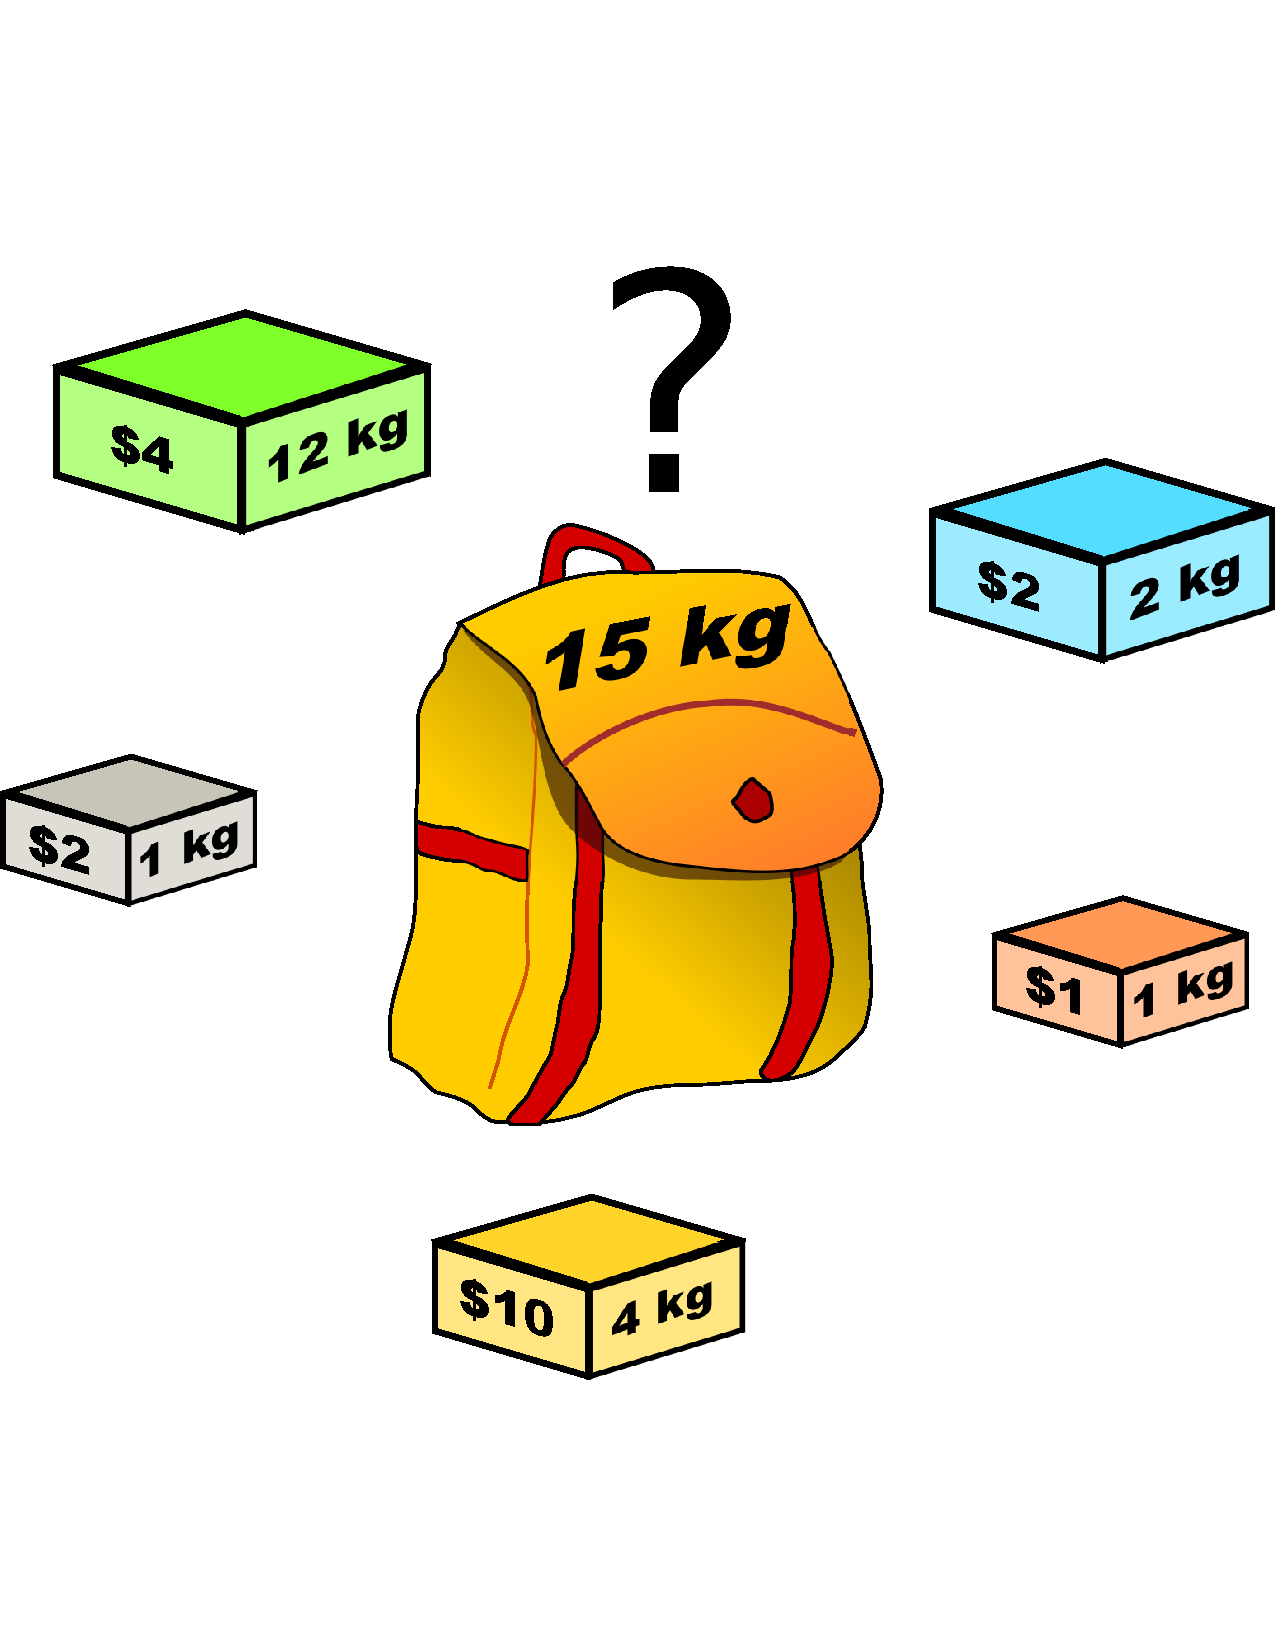
\includegraphics[scale = 0.2]{knapsack}\footnotemark 
%\end{center}
%\label{fig:knapsack}
%\caption{Knapsack Problem: which items should we choose take in the knapsack that maximizes the value while respecting the 15kg weight limit?}
%\end{figure}
%\footnotetext{\url{https://en.wikipedia.org/wiki/Knapsack_problem}}

\begin{examplewithcode}{Knapsack}{https://github.com/open-optimization/open-optimization-or-examples/blob/master/integer-programming/knapsack-problem.ipynb}
\label{example:knapsack}
You have a knapsack (bag) that can only hold W = 15 kgs.  There are 5 items that you could possibly put into your knapsack.  The items (weight, value) are given as:
(12 kg, $\$$4), (2 kg, $\$$2), (1kg, $\$$2), (1kg, $\$$1), (4kg, $\$$10).  Which items should you take to maximize your value in the knapsack? See \autoref{fig:wiki/File/knapsack}.\\

\noindent \textbf{Variables:}
\begin{itemize}
\item let $x_i = 0$ if item $i$ is in the bag
\item let $x_i = 1$ if item $i$ is not in the bag
\end{itemize}
\textbf{Model:}
\begin{align}
\max  \  \ &4 x_1 + 2 x_2 + 2 x_3 + 1 x_4 + 10 x_5 \tag{Total value}\\
\text{ s.t. }\ \ &  12 x_1 + 2 x_2 + 1 x_3 + 1 x_4 + 4 x_5 \leq 15 \tag{Capacity bound}\\
& x_i \in \{0,1\} \text{ for } i=1, \dots, 5 \tag{Item taken or not}
\end{align}
\end{examplewithcode}
In the integer case, we typically require the variables to be non-negative integers, hence we use the notation $x \in \Z^n_+$.  This setting reflects the fact that instead of single individual items, you have item types of which you can take as many of each type as you like that meets the constraint.
\begin{general}{Integer Knapsack Problem}{\npcomplete}
Given an non-negative weight vector $a \in \Q^n_+$, a capacity $b \in \Q_+$, and objective coefficients $c \in \Q^n$, 
\begin{equation}
\begin{split}
\max \ \ & c^\top x\\
\text{s.t.}\ \ & a^\top x \leq b\\
& x \in \Z^n_+
\end{split}
\end{equation}
\end{general}
We can also consider an equality constrained version
\begin{general}{Equality Constrained Integer Knapsack Problem}{\nphard}
Given an non-negative weight vector $a \in \Q^n_+$, a capacity $b \in \Q_+$, and objective coefficients $c \in \Q^n$, 
\begin{align}
\max \ \ & c^\top x\\
\text{s.t.}\ \ & a^\top x = b\\
& x \in \Z^n_+
\end{align}
\end{general}
\begin{example}
\label{ex:min-coins}
Using pennies, nickels, dimes, and quarters, how can you minimize the number of coins you need to to make up a sum of $83\cent$? 

\textbf{Variables:}
\begin{itemize}
\item Let $p$ be the number of pennies used
\item Let $n$ be the number of nickels used
\item Let $d$ be the number of dimes used
\item Let $q$ be the number of quarters used
\end{itemize}
\textbf{Model}
\begin{align*}
\min \quad & p + n + d + q & \text{ total number of coins used}\\
\text{ s.t. } \quad & p + 5n + 10d + 25 q = 83 & \text{sums to } 83 \cent\\
& p,d,n,q \in \Z_+ & \text{each is a non-negative integer}
\end{align*}
\end{example}
\section{Capital Budgeting}
\todoSection{}

% Copywrite Robert Hildeband 2019

The \emph{capital budgeting} problem is a nice generalization of the knapsack problem.   This problem as the same structure as the knapsack problem, except now it has multiple constraints.   We will first describe the problem, give a general model, and then look at an explicit example.

\begin{general}{Capital Budgeting}{}
\label{general:capital-budgeting}
A firm has $n$ projects it could undertake to maximize revenue, but budget limitations require that not all can be completed.
\begin{itemize}
\item Project $j$ expects to produce revenue $c_j$ dollars overall.
\item Project $j$ requires investment of $a_{ij}$ dollars in time period $i$ for $i = 1,\ldots,m$.
\item The capital available to spend in time period $i$ is $b_i$.
\end{itemize}
Which projects should the firm invest in to maximize it's expected return while satisfying it's weekly budget constriaints?
\end{general}

\newpage

We will first provide a general formulation for this problem.

\begin{general}{Capital Budgeting Model}{}
\noindent \textbf{Sets:}
\begin{itemize}
\item Let $I = \{1, \dots, m\}$ be the set of time periods.
\item Let $J = \{1, \dots, n\}$ be the set of possible investments.
\end{itemize}

\noindent \textbf{Parameters:}
\begin{itemize}
\item $c_j$ is the expected revenue of investment $j$ for $j \in J$
\item $b_i$ is the available capital in time period $i$ for $i$ in  $I$
\item $a_{ij}$ is the resources required for invesment $j$ in time period $i$, for $i$ in $I$, for $j$ in $J$.
\end{itemize}

\noindent \textbf{Variables:}
\begin{itemize}
\item let $x_i = 0$ if investment $i$ is chosen
\item let $x_i = 1$ if investment $i$ is not chosen
\end{itemize}
\textbf{Model:}
\begin{align*}
	\max ~~~& \sum_{j = 1}^n c_jx_j \tag{Total Expected Revenue}\\
	s.t. ~~~&\sum_{j = 1}^n a_{ij}x_j\leq b_i, ~~~i = 1,\ldots m  \tag{ Resource constraint week $i$}\\
	& x_j \in \{0,1\} , \ j = 1,\ldots,n
	\end{align*}

\end{general}


\newpage
%\begin{examplewithcode}{Capital Budgeting}{code:capital-budgeting}
%\label{example:capital-budgeting}
Consider the example given in the following table.
	\begin{table}[h]
			\begin{tabular}{|c|c|c|c|}%[<+->]
				\hline
				Project & $\mathbb{E}$[Revenue] & Resources required in week 1 & Resources required in week 2\\\hline
				\rowcolor{gray!10} 1 & 10 & 3 & 4\\
				\hline
				2 & 8 & 1 & 2\\\hline
				\rowcolor{gray!10} 3 & 6 & 2 & 1\\
				\hline
				Resources available & & 5 & 6\\
				\hline
		\end{tabular}
	\end{table}


Given this data, we can setup our problem explicitly as follows

\begin{examplewithcode}{Capital Budgeting}{https://github.com/open-optimization/open-optimization-or-examples/blob/master/integer-programming/capital-budgeting.ipynb}
\noindent \textbf{Sets:}
\begin{itemize}
\item Let $I = \{1,2\}$ be the set of time periods.
\item Let $J = \{1, 2,3\}$ be the set of possible investments.
\end{itemize}

\noindent \textbf{Parameters:}
\begin{itemize}
\item $c_j$ is given in column "$\mathbb{E}$[Revenue]".
\item $b_i$ is given in row "Resources available".
\item $a_{ij}$ given in row $j$, and column for week $i$.
\end{itemize}

\noindent \textbf{Variables:}
\begin{itemize}
\item let $x_i = 0$ if investment $i$ is chosen
\item let $x_i = 1$ if investment $i$ is not chosen
\end{itemize}

The explict model is given by\\
\noindent  \textbf{Model:}
\begin{align*}
	\max\ \ \  & 10x_1+8x_2+6x_3 \tag{Total Expected Revenue}\\
	s.t. \ \ & 
	3x_1+1x_2+2x_3\leq5 \tag{ Resource constraint week 1}\\
	&4x_1+2x_2+1x_3\leq6 \tag{ Resource constraint week 2}\\
&x_j \in \{0,1\},\  j = 1,2,3
\end{align*}

\end{examplewithcode}




\section{Set Covering}
\todoSection{}

The \emph{set covering} problem can be used for a wide array of problems.    We will see several examples in this section.

\begin{general}{Set Covering}{\npcomplete}
\label{general:set-covering}
Given a set $V$ with subsets $V_1, \dots, V_l$, determine the smallest subset $S \subseteq V$ such that 
$S \cap V_i \neq \emptyset$ for all $i=1, \dots, l$.

The set cover problem can be modeled as
\begin{equation}
\begin{split}
\min \ \ & \one^\top x\\
\text{s.t.} \ \ & \sum_{v \in V_i} x_v \geq 1 \text{ for all } i =1, \dots, l \\ 
& x_v \in \{0,1\} \text{ for all } v \in V
\end{split}
\end{equation}
where $x_v$ is a 0/1 variable that takes the value $1$ if we include item $j$ in set $S$ and $0$ if we do not include it in the set $S$.  
\end{general}



\todo[inline]{
Add flight crew scheduling example and images.
}

\begin{examplewithcode}{Capital Budgeting}{https://github.com/open-optimization/open-optimization-or-examples/blob/master/integer-programming/capital-budgeting.ipynb}
\noindent \textbf{Sets:}
\begin{itemize}
\item Let $I = \{1,2\}$ be the set of time periods.
\item Let $J = \{1, 2,3\}$ be the set of possible investments.
\end{itemize}

\noindent \textbf{Parameters:}
\begin{itemize}
\item $c_j$ is given in column "$\mathbb{E}$[Revenue]".
\item $b_i$ is given in row "Resources available".
\item $a_{ij}$ given in row $j$, and column for week $i$.
\end{itemize}

\noindent \textbf{Variables:}
\begin{itemize}
\item let $x_i = 0$ if investment $i$ is chosen
\item let $x_i = 1$ if investment $i$ is not chosen
\end{itemize}

The explict model is given by\\
\noindent  \textbf{Model:}
\begin{align*}
	\max\ \ \  & 10x_1+8x_2+6x_3 \tag{Total Expected Revenue}\\
	s.t. \ \ & 
	3x_1+1x_2+2x_3\leq5 \tag{ Resource constraint week 1}\\
	&4x_1+2x_2+1x_3\leq6 \tag{ Resource constraint week 2}\\
&x_j \in \{0,1\},\  j = 1,2,3
\end{align*}

\end{examplewithcode}




One specific type of set cover problem is the \emph{vertex cover} problem.
\begin{general}{Example: Vertex Cover}{\npcomplete}
\label{ex:vertex-cover}
Given a graph $G = (V,E)$ of vertices and edges, we want to find a smallest size subset $S \subseteq V$ such that every for every $e = (v,u) \in E$, either $u$ or $v$ is in $S$.   

We can write this as a mathematical program in the form:
\begin{equation}
\begin{split}
\min \ \ & \one^\top x\\
\text{s.t.} \ \ & x_u + x_v \geq 1 \text{ for all } (u,v) \in E \\ 
& x_v \in \{0,1\} \text{ for all } v \in V.
\end{split}
\end{equation}
\end{general}




\begin{examplewithcode}{Set cover: Fire station placement}{https://github.com/open-optimization/open-optimization-or-examples/blob/master/integer-programming/fire-station-covering.ipynb}
\label{example:fire-station}

In the fire station problem, we seek to choose locations for fire stations such that any district either contains a fire station, or neighbors a district that constains a fire station.  Figure~\ref{fig:tikz/Illustration1.pdf} depicts the set of districts and an example placement of locations of fire stations.  How can we minimize the the total number of fire stations that we need?


\noindent \textbf{Sets:}
\begin{itemize}
\item Let $V$ be the set of districts ($V = \{1, \dots, 16\}$)
\item Let $V_i$ be the set of districts that neighbor district $i$ (e.g. $V_1 = \{2,4,5\}$).
\end{itemize}

\noindent \textbf{Variables:}
\begin{itemize}
\item let $x_i = 1$ if district $i$ is chosen to have a fire station.
\item let $x_i = 0$ otherwise.
\end{itemize}
\textbf{Model:}
\begin{align}
\min  \  \ &\sum_{i \in V} x_i \tag{ \# \text{ open fire stations}}\\
\text{ s.t. }\ \ &  x_i + \sum_{j \in V_i} x_j \geq 1 & \forall{i \in V} \tag{Station proximity requirement}\\
& x_i \in \{0,1\} & \text{ for } i\in V  \tag{station either open or closed}
\end{align}
\end{examplewithcode}

\includefiguresource[Layout of districts and possible locations of fire stations.][][h]{tikz/Illustration1.pdf}
\includefiguresource[Set cover representation of fire station problem.  For example, choosing district 16 to have a fire station covers districts 13, 15, and 16.]{tikz/Illustration2.pdf}
\includefiguresource[Graph representation of fire station problem.  Every node is connected to a chosen node by an edge]{tikz/Illustration3.pdf}



%\documentclass[../open-optimization/open-optimization.tex]{subfiles}

%%%%%%%%%
%\begin{document}
%%%%%%%%%

\begin{general}{Set Covering - Matrix description}{\npcomplete}
\label{general:set-covering-alternate}
Given a non-negative matrix $A \in \{0,1\}^{m \times n}$, a non-negative vector, and an objective vector $c \in \R^n$, the set cover problem is
\begin{equation}
\begin{split}
\max \ \ & c^\top x\\
\text{s.t.}. \ \ & Ax \geq \one \\
& x \in \{0,1\}^n.
\end{split}
\end{equation}
\end{general}
\begin{examplewithoutcode}{Vertex Cover with matrix}{code:vertex-cover-matrix}
An alternate way to solve \nameref{ex:vertex-cover} is to define the \emph{adjacency matrix} $A$ of the graph.  The adjacency matrix is a $|E| \times |V|$ matrix with $\{0,1\}$ entries.  The each row corresponds to an edge $e$ and each column corresponds to a node $v$.  For an edge $e = (u,v)$, the corresponding row has a $1$ in columns corresponding to the nodes $u$ and $v$, and a 0 everywhere else.  Hence, there are exactly two 1's per row.  Applying the formulation above in \nameref{general:set-covering-alternate} models the problem.
\end{examplewithoutcode}




%%%%%%%%%
%\end{document}
%%%%%%%%%




\subsection{Covering (Generalizing Set Cover)}
We could also allow for a more general type of set covering where we have non-negative integer variables and a right hand side that has values other than $1$.
\begin{general}{Covering}{\npcomplete}
\label{general:covering}
Given a non-negative matrix $A \in \Z_+^{m \times n}$, a non-negative vector $b \in \Z^m$, and an objective vector $c \in \R^n$, the set cover problem is
\begin{equation}
\begin{split}
\max \ \ & c^\top x\\
\text{s.t.}. \ \ & Ax \geq b \\
& x \in\Z^n_+.
\end{split}
\end{equation}
\end{general}

%\todo[inline]{
% Add Nurse scheduling problem.
%}
%
%\begin{examplewithcode}{Nurse Scheduling}{code:nurse-scheduling}
%Suppose that we have $n$ full-time nurses employed and $p$ part-time nurses employed.  We need to schedule nurses such that, for each day of the week, we have enough nurses on hand to cover all the tasks.  
%
%\todo[inline]{Add complete example}
%\end{examplewithcode}




\section{Assignment Problem}
\todoSection{}
The \emph{assignment problem} (machine/person to job/task assignment) seeks to assign tasks to machines in a way that is most efficient.   This problem can be thought of as having a set of machines that can complete various tasks (textile machines that can make t-shirts, pants, socks, etc) that require different amounts of time to complete each task, and given a demand, you need to decide how to alloacte your machines to tasks.

Alternatively, you could be an employer with a set of jobs to complete and a list of employees to assign to these jobs.  Each employee has various abilities, and hence, can complete jobs in differing amounts of time.  And each employee's time might cost a different amout.  How should you assign your employees to jobs in order to minimize your total costs?


\begin{general}{Assignment Problem}{}{}
Given $m$ machines and $n$ jobs, find a least cost assignment of jobs to machines. The cost of assigning job $j$ to machine $i$ is $c_{ij}$.
\end{general}

\todo[inline]{
Include picture and example data
}


\begin{examplewithcode}{Machine Assignment}{https://github.com/open-optimization/open-optimization-or-examples/blob/master/integer-programming/assignment-problem.ipynb}
\noindent \textbf{Sets:}
\begin{itemize}
\item Let $I = \{0,1,2,3\}$ set of machines.
\item Let $J = \{0,1, 2,3\}$ be the set of tasks.
\end{itemize}

\noindent \textbf{Parameters:}
\begin{itemize}
\item $c_{ij}$ - the cost of assigning machine $i$ to job $j$
%\item $c_j$ is given in column "$\mathbb{E}$[Revenue]".
%\item $b_i$ is given in row "Resources available".
%\item $a_{ij}$ given in row $j$, and column for week $i$.
\end{itemize}

\noindent \textbf{Variables:}
\begin{itemize}
\item Let 
\begin{equation*}
x_{ij} = \begin{cases}
1 & \text{if machine $i$ assigned to job $j$}\\
0 & \text{otherwise.}
\end{cases}
\end{equation*}
%\item let $x_i = 1$ if investment $i$ is not chosen
\end{itemize}

\noindent  \textbf{Model:}
\begin{align*}
	\min\ \ \  & \sum_{i \in I, j \in J} c_{ij} x_{ij} \tag{Minimize cost}\\
	s.t. \ \ & \sum_{i \in I} x_{ij} = 1 & \text{for all $j \in J$}
	 \tag{All jobs are assigned one machine}\\
	& \sum_{j \in J} x_{ij} = 1 & \text{for all $i\in I$}
	 \tag{All machines are assigned to a job}\\
	 & x_{ij} \in \{0,1\} \forall i \in I, j \in J
	  \end{align*}
\end{examplewithcode}



\section{Facility Location}
\todoSection{}
The basic model of the facility location problem is to determine where to place your stores or facilities in order to be close to all of your customers and hence reduce the costs transportation to your customers.  Each customer is known to have a certain demand for a product, and each facility has a capacity on how much of that demand it can satisfy.  Furthermore, we need to consider the cost of building the facility in a given location.

This basic framework can be applied in many types of problems and there are a number of variants to this problem.   We will address two variants: the \emph{capacitated facility location problem} and the \emph{uncapacitated facility location problem}.  
\todo[inline]{
Add discussion on Facility Location Problems and pictures.
}



\subsection{Capacitated Facility Location}

\begin{general}{Capacitated Facility Location}{\npcomplete}
Given costs connections $c_{ij}$ and fixed building costs $f_i$, demands $d_j$ and capacities $u_i$, the capacitated facility location problem is 

\noindent \textbf{Sets:}
\begin{itemize}
\item Let $I = \{1,\dots, n\}$ be the set of facilities.
\item Let $J = \{1, \dots, m\}$ be the set of customers.
\end{itemize}

\noindent \textbf{Parameters:}
\begin{itemize}
\item $f_i$ - the cost of opening facility $i$.
\item $c_{ij}$ - the cost of fulfilling the complete demand of customer $j$ from facility $i$.
\item $u_{i}$ - the capacity of facility $i$.
\item $d_{j}$ - the demand by customer $j$.
%\item $c_j$ is given in column "$\mathbb{E}$[Revenue]".
%\item $b_i$ is given in row "Resources available".
%\item $a_{ij}$ given in row $j$, and column for week $i$.
\end{itemize}

\noindent \textbf{Variables:}
\begin{itemize}
\item Let 
\begin{equation*}
y_{i} = \begin{cases}
1 & \text{if we open facility $i$,}\\
0 & \text{otherwise.}
\end{cases}
\end{equation*}
\item Let $x_{ij} \geq 0$ be the fraction of demand of customer $j$ satisfied by facility $i$.
%\item let $x_i = 1$ if investment $i$ is not chosen
\end{itemize}

\noindent  \textbf{Model:}
\begin{align}
\min & \displaystyle\sum_{i=1}^n\sum_{j=1}^mc_{ij}x_{ij}+\sum_{i=1}^nf_iy_i \tag{total cost}\\
\text{s.t.} & \displaystyle\sum_{i=1}^nx_{ij}=1 \text{ for all }j=1,\dots,m \tag{assign demand to facility}\\
& \displaystyle \sum_{j=1}^md_jx_{ij}\leqslant u_iy_i\text{ for all }i=1\dots,n \tag{capacity of facility $i$}\\
&x_{ij}\geqslant0\text{ for all }i=1,\dots,n \text{ and }j=1,\dots,m \tag{nonnegative fraction of demand satisfied}\\
&y_i\in\{0,1\}\text{ for all } i=1,\dots,n \tag{open/not open facility}
\end{align}

\end{general}

Alternative model!

\begin{align*}
\min \ \ \ & \sum_{i = 1}^m\sum_{j=1}^n c_{ij}x_{ij}+\sum_{i = 1}^mf_iy_i\\
s.t.&  \sum_{i = 1}^mx_{ij} = 1,~~~~~j =1,\ldots n\\
& \displaystyle \sum_{j=1}^md_jx_{ij}\leqslant u_i\text{ for all }i=1\dots,n \tag{capacity of facility $i$}\\
&x_{ij}\leq y_i,~~~~~ i = 1,\ldots m,~~~ j = 1,\ldots,n\\
&  x_{ij} \geq 0~~~~~ i = 1,\ldots,m, ~~~j = 1,\ldots,n\\
& y_i\in \{0,1\}, \  \  i = 1,\ldots,m
\end{align*}

\subsection{Uncapacitated Facility Location}
\begin{general}{Uncapacitated Facility Location}{\npcomplete}
Given costs connections $c_{ij}$ and fixed building costs $f_i$, the uncapacitated facility location problem is 
\begin{equation}
\begin{array}{rl}
\min & \displaystyle\sum_{i=1}^n\sum_{j=1}^mc_{ij}z_{ij}+\sum_{i=1}^nf_ix_i \\
\text{s.t.} & \displaystyle\sum_{i=1}^nz_{ij}=1 \text{ for all }j=1,\dots,m \\
& \displaystyle \sum_{j=1}^mz_{ij}\leqslant Mx_i\text{ for all }i=1\dots,n \\
&z_{ij}\in\{0,1\}\text{ for all }i=1,\dots,n \text{ and }j=1,\dots,m\\
&x_i\in\{0,1\}\text{ for all } i=1,\dots,n
\end{array}
\end{equation}
Here $M$ is a large number and can be chosen as $M = m$, but could be refined smaller if more context is known.
\end{general}

Alternative model!

\begin{equation}
\begin{array}{rl}
\min & \displaystyle\sum_{i=1}^n\sum_{j=1}^mc_{ij}z_{ij}+\sum_{i=1}^nf_ix_i \\
\text{s.t.} & \displaystyle\sum_{i=1}^nz_{ij}=1 \text{ for all }j=1,\dots,m \\
& z_{ij}\leqslant x_i\text{ for all }i=1\dots,n \text{ for all } j = 1, \dots, m \\
&z_{ij}\in\{0,1\}\text{ for all }i=1,\dots,n \text{ and }j=1,\dots,m\\
&x_i\in\{0,1\}\text{ for all } i=1,\dots,n
\end{array}
\end{equation}
\newpage
\section{Basic Modeling Tricks - Using Binary Variables}
%\todoSection{}
In this section, we describe ways to model a variety of constraints that commonly appear in practice.  The goal is changing constraints described in words to constraints defined by math.

Binary variables can allow you to model many types of constraints.  We discuss here varios logical constraints where we assume that $x_i \in \{0,1\}$ for $i=1, \dots, n$.  We will take the meaning of the variable to be selecting an item.

\begin{enumerate}
 \item If item $i$ is selected, then item $j$ is also selected.
 \begin{equation}
 x_i \leq x_j
 \end{equation}
 \begin{enumerate}
 \item If any of items $1, \dots, 5$ are selected, then item $6$ is selected.
 \begin{equation}
 x_1 + x_2 + \dots + x_5 \leq 5 \cdot x_6
 \end{equation}
 Alternatively!
 \begin{equation}
 x_i \leq x_6 \ \ \ \ \text{ for all } i=1, \dots, 5
 \end{equation}
 \end{enumerate}
 \item If item $j$ is not selected, then item $i$ is not selected.
 \begin{equation}
x_i \leq x_j
 \end{equation}
  \begin{enumerate}
 \item If item $j$ is not selected, then all items $1, \dots, i$ are not selected.
 \begin{equation}
 x_1 + x_2 + \dots + x_i \leq i \cdot x_j
 \end{equation}
 \end{enumerate}
  \item If item $j$ is not selected, then item $i$ is not selected.
 \begin{equation}
x_i \leq x_j
 \end{equation}
\item Either item $i$ is selected or item $j$ is selected, but not both.
 \begin{equation}
 x_i + x_j = 1
 \end{equation}
\item Item $i$ is selected or item $j$ is selected or both.
 \begin{equation}
 x_i + x_j \geq 1
 \end{equation}
\item If item $i$ is selected, then item $j$ is not selected.
 \begin{equation}
x_j \leq (1-x_i)
 \end{equation}

\item At most one of items $i ,j$, and $k$ are selected.
 \begin{equation}
 x_i + x_j + x_k \leq 1
 \end{equation}
\item At most two of items $i,j,$ and $k$ are selected.
 \begin{equation}
 x_i + x_j + x_k \leq 2
 \end{equation}
\item Exactly one of items $i,j,$ and $k$ are selected.
 \begin{equation}
  x_i + x_j + x_k = 1
 \end{equation}
\end{enumerate}

These tricks can be connected to create different function values.  

\begin{example}{Variable takes one of three values}{}
Suppose that the variable $x$ should take one of the three values $\{4, 8, 13\}$. This can be modeled using three binary variables as
\begin{align*}
x=4z_1 +8z_2 +13z_3\\
 z_1 +z_2 +z_3 =1\\
z_i \in \{0, 1\} \text{ for } i = 1, 2,3.
\end{align*}
As a convenient addition, if we want to add the possibility that it takes the value $0$, then we can model this as 
\begin{align*}
x=4z_1 +8z_2 +13z_3\\
 z_1 +z_2 +z_3 \leq 1\\
z_i \in \{0, 1\} \text{ for } i = 1, 2,3.
\end{align*}
\end{example}


We can also model variable increases at different amounts.  \begin{example}{Discount for buying more}{}
Suppose you can choose to buy 1, 2, or 3 units of a product, each with a decreasing cost.  The first unit is \$10, the second is \$5, and the third unit is \$3.
\begin{align*}
x=10z_1 +5z_2 +3z_3\\
 z_1\geq z_2 \geq z_3\\
z_i \in \{0, 1\} \text{ for } i = 1, 2,3.
\end{align*}
Here, $z_i$ represents if we buy the $i$th unit.  The inequality constraints impose that if we buy unit $j$, then we must by all units $i$ with $i < j$.
\end{example}



In this section, we describe ways to model a variety of constraints that commonly appear in practice.  The goal is changing constraints described in words to constraints defined by math.
\subsection{Big M constraints - Activating/Deactivating Inequalities}
Big M comes again!   It's extremely useful when trying to activate constrants based on a binary variable.

For intance, if we don't rent a bus, then we can have at most 3 passengers join us on our trip.   Consider passengers $A,B,C,D,E$ and let $x_i \in \{0,1\}$ be 1 if we take passenger $i$ and 0 otherwise.
We can model the constraint that we can have at most 5 passengers as 
$$
x_A + x_B + x_C + x_D + x_E \leq 3.
$$

We want to be able to activate this constraint in the event that we don't rent a bus.

Let $\delta \in \{0,1\}$ be 1 if rent a bus, and 0 otherwise.  

Then we want to say
\begin{quote}
If $\delta = 0$ , then 
$$
x_A + x_B + x_C + x_D + x_E \leq 3.
$$
\end{quote}

We can formulate this using a big-M constraint as

\begin{equation}
x_A + x_B + x_C + x_D + x_E \leq 3 + M \delta.
\end{equation}

Notice the two case
$$
\begin{cases}
x_A + x_B + x_C + x_D + x_E \leq 3  & \text{ if } \delta = 0\\
x_A + x_B + x_C + x_D + x_E \leq 3 +M & \text{ if } \delta = 1
\end{cases}
$$
In the second case, we choose $M$ to be so large, that the second case inequality is vacuous.    That said, choosing smaller $M$ values (that are still valid) will help the computer program solve the problem faster.  In this case, it suffices to let $M = 2$.

We can speak about this technique more generally as
\begin{general}{Big-M: If then}{}{}
We aim to model the relationship
\begin{equation}
\text{ If } \ \ \   \delta = 0, \ \ \  \text{then  } \ \ \ a^\top x \leq b.
\end{equation}
By letting $M$ be an upper bound on the quantity $a^\top x - b$, we can model this condition as 
\begin{equation}
\begin{split}
a^\top x - b& \leq M\delta\\
\delta & \in \{0,1\}
\end{split}
\end{equation}
\end{general}


\subsection{Either Or Constraints}
\emph{``At least one of these constraints holds"} is what we would like to model.  Equivalently, we can phrase this as an \emph{inclusive or} constraint.  This can be molded with a pair of Big-M constraints.
\begin{general}{Either Or}{}{}

\begin{equation}
\text{Either} \ \ \ a^\top x \leq b\ \  \text{  or  } \ \  c^\top x \leq d \ \ \text{holds} 
\end{equation}
can be modeled as 
\begin{equation}
\begin{split}
a^\top x - b &\leq M_1 \delta\\
c^\top x - d &\leq M_2 (1-\delta)\\
\delta &\in \{0,1\},
\end{split}
\end{equation}
where $M_1$ is an upper bound on $a^\top x - b$ and $M_2$ is an upper bound on $c^\top x - d$.
\end{general}

\begin{example}{}{}
Either $2$ buses or $10$ cars are needed shuttle students to the football game.  
\begin{itemize}
\item Let $x$ be the number of buses we have and 
\item let $y$ be the number of cars that we have.  
\end{itemize}
Suppose that there are at most $M_1 = 5$ buses that could be rented an at most $M_2 = 20$ cars that could be available.

This constraint can be modeled as 
\begin{equation}
\begin{split}
x - 2 &\leq 5\delta\\
y - 10 &\leq 20 (1-\delta)\\
\delta &\in \{0,1\},
\end{split}
\end{equation}
\end{example}
\subsection{If then implications - opposite direction}
Suppose that we want to model the fact that if we have at most 10 students attending this course, then we must switch to a smaller classroom.   

Let $x_i \in \{0,1\}$ be 1 if student $i$ is in the course or not.   Let $\delta \in \{0,1\}$ be 1 if we need to switch to a smaller classroom.  

Thus, we want to model 
\begin{quote}
If $$
\sum_{i \in I} x_i \leq 10
$$
then 
$$
\delta = 1.
$$
\end{quote}

We can model this as 
\begin{equation}
\sum_{i \in I} x_i \geq 10 + 1 + M\delta.
\end{equation}


\begin{general}{If inequality, then indicator}
We let $m$ be a lower bound on the quantity $a^\top x - b$ and we let $\epsilon$ be a tiny number that is an error bound in verifying if an inequality is violated.  \textbf{If the data $a,b$ are integer and $x$ is an integer, then we can take $\epsilon = 1$.}

Now
\begin{equation}
\text{If } \ \ a^\top x \leq b  \ \ \text{then}\ \ \delta = 1
\end{equation}
can be modeled as 
\begin{equation}
a^\top x -b  \geq  \epsilon(1-\delta) + m \delta.
\end{equation}
\end{general}



\begin{proof}We not justify the statement above.

A simple way to understand this constraint is to consider the \emph{contrapositive} of the if then statement that we want to model.  The contrapositive says that 
\begin{equation}
\text{If $\delta = 0$, then $a^\top x - b > 0$.}
\end{equation}
To show the contrapositive, we set $\delta = 0$.  Then the inequality becomes 
$$
a^\top x - b \geq \epsilon(1-0) + m0 = \epsilon > 0.
$$
Thus, the contrapositive holds.

\textbf{If instead we wanted a direct proof:}

Case 1: Suppose $a^\top x \leq b$.  Then $0 \geq a^\top x - b$, which implies that 
$$
\delta(a^\top x - b) \geq a^\top x - b
$$
Therefore
$$
\delta(a^\top x - b) \geq \epsilon(1-\delta) + m \delta
$$
After rearranging
$$
\delta(a^\top x - b - m) \geq \epsilon(1-\delta)
$$
Since $a^\top x - b - m \geq 0$ and $\epsilon > 0$, the only feasible choice is $\delta = 1$.


Case 2:  Suppose $a^\top x > b$.  Then $a^\top x - b \geq \epsilon$.    Since $a^\top x -b \geq m$, both choices $\delta = 0$ and $\delta = 1$ are feasible.

By the choice of $\epsilon$,  we know that $a^\top x -b > 0$ implies that $a^\top x - b \geq \epsilon$.  



Since we don't like strict inequalities, we write the strict inequality as $a^\top x - b \geq \epsilon$ where $\epsilon$ is a small positive number that is a smallest difference between $a^\top x - b$ and $0$ that we would typically observe.  As mentioned above, if $a,b,x$ are all integer, then we can use $\epsilon = 1$.

Now we want an inequality with left hand side $a^\top x - b \geq$ and right hand side to take the value 
\begin{itemize}
\item $\epsilon$ if $\delta = 0$,
\item $m$ if $\delta = 1$.
\end{itemize}
This is accomplished with right hand side $\epsilon (1-\delta) + m\delta$.
\end{proof}

Many other combinations of if then statements are summarized in the following table:
\begin{table}
\begin{center}
\begin{tabular}{|c|c|}
\hline
\textbf{Implication} & \textbf{Constraint}\\
\hline
If $\delta = 0$, then $a^\top x \leq b$ & $a^\top x \leq b + M \delta$\\
If $a^\top x \leq b$, then $\delta = 1$ & $a^\top x \geq m \delta + \epsilon(1-\delta)$\\
\hline
\end{tabular}
\end{center}
\caption{Short list: If/then models with a constraint and a binary variable.  Here $M$ and $m$ are upper and lower bounds on $a^\top x - b$ and $\epsilon$ is a small number such that if $a^\top x > b$, then $a^\top x \geq b + \epsilon$.}
\end{table}
These two implications can be used to derive the following longer list of implications.

\begin{table}
\begin{center}
\begin{tabular}{|c|c|}
\hline
\textbf{Implication} & \textbf{Constraint}\\
\hline
If $\delta = 0$, then $a^\top x \leq b$ & $a^\top x \leq b + M \delta$\\
If $\delta = 0$, then $a^\top x \geq b$ & $a^\top x \geq b + m \delta$\\
If $\delta = 1$, then $a^\top x \leq b$ & $a^\top x \leq b + M (1-\delta)$\\
If $\delta = 1$, then $a^\top x \geq b$ & a$^\top x \geq b + m (1-\delta)$\\
If $a^\top x \leq b$, then $\delta = 1$ & $a^\top x \geq b + m \delta + \epsilon(1-\delta)$\\
If $a^\top x \geq b$, then $\delta = 1$ & $a^\top x \leq b + M \delta - \epsilon(1-\delta)$\\
If $a^\top x \leq b$, then $\delta = 0$ & $a^\top x \geq b + m (1-\delta) + \epsilon \delta$\\
If $a^\top x \geq b$, then $\delta = 0$ & $a^\top x \geq b + m (1-\delta) - \epsilon \delta$\\
\hline
\end{tabular}
\end{center}
\caption{Long list: If/then models with a constraint and a binary variable.  Here $M$ and $m$ are upper and lower bounds on $a^\top x - b$ and $\epsilon$ is a small number such that if $a^\top x > b$, then $a^\top x \geq b + \epsilon$.}
\end{table}
Lastly, if you insist on having exact correspondance, that is, "$\delta = 0 $ if and only if $a^\top x \leq b$" you can simply include both constraints for "if $\delta = 0 $, then $a^\top x \leq b$" and if "$a^\top x \leq b$, then $\delta = 0 $".  Although many problems may be phrased in a way that suggests you need "if and only if", it is often not necessary to use both constraints due to the objectives in the problem that naturally prevent one of these from happening.  

For example, if we want to add a binary variable $\delta$ that means
$$
\begin{cases}
\delta = 0 \text{ implies }  a^\top x \leq b\\
\delta = 1  \text{ Otherwise}
\end{cases}
$$
If $\delta = 1$ does not effect the rest of the optimization problem, then adding the constraint regarding $\delta = 1$ is not necessary.  Hence, typically, in this scenario, we only need to add the constraint $a^\top x \leq b + M \delta$.

\subsection{Binary reformulation of integer variables}
If an integer variable has small upper and lower bounds, it can sometimes be advantageous to recast it as a sequence of binary variables - for either modeling, the solver, or both.   Although there are technically many ways to do this, here are the two most common ways.

\begin{general}{Full reformulation}{\textcolor{blue}{$u$ many binary variables}}
\label{general:full-reformulation}
For a non-negative integer variable $x$ with upper bound $u$, modeled as 
\begin{equation}
0 \leq x \leq u, \ \ \ \ x \in \Z,
\end{equation}
this can be reformulated with $u$ binary variables $z_1, \dots, z_u$ as 
\begin{equation}
\begin{split}
x & = \sum_{i=1}^u i z_i = z_1 + 2 z_2 + \dots + u z_u\\
1 & \geq \sum_{i=1}^u z_i = z_1 + z_2 + \dots + z_u\\
z_i & \in \{0,1\} \ \ \text{ for } i=1, \dots, u
\end{split}
\end{equation}
\end{general}
We call this the \emph{full reformulation} because there is a binary variable $z_i$ associated with every value $i$ that $x$ could take.  That is, if $z_3 = 1$, then the second constraint forces $z_i = 0$ for all $i \neq 3$ (that is, $z_3$ is the only non-zero binary variable), and hence by the first constraint, $x = 3$.

\begin{general}{Binary reformulation}{\textcolor{blue}{$O(\log u)$ many binary variables}}
\label{general:log-reformulation}
For a non-negative integer variable $x$ with upper bound $u$, modeled as 
\begin{equation}
0 \leq x \leq u, \ \ \ \ x \in \Z,
\end{equation}
this can be reformulated with $u$ binary variables $z_1, \dots, z_{\lfloor\log( u )\rfloor}$ as 
\begin{equation}
\begin{split}
x & = \sum_{i=0}^{\lfloor\log( u )\rfloor}2^i z_i = z_0 + 2 z_1 +  4 z_2 + 8 z_3 + \dots + 2^{\lfloor\log( u )\rfloor} z_{\lfloor\log( u )\rfloor}\\
z_i & \in \{0,1\} \ \ \text{ for } i=1, \dots, \lfloor\log( u )\rfloor
\end{split}
\end{equation}
\end{general}
We call this the \emph{log reformulation} because this requires only logarithmically many binary variables in terms of the upper bound $u$.   This reformulation is particularly better than the full reformulation when the upper bound $u$ is a ``larger" number, although we will leave it ambiguous as to how larger a number need to be in order to be described as a ``larger" number. 
\subsection{SOS1 Constraints}
\begin{definition}{Special Ordered Sets of Type 1 (SOS1)}
A Special Ordered Sets of type 1 (SOS1) constraint on a vector indicates that \emph{at most one element of the vector can non-zero}.
\end{definition}
We next give an example of how to use binary variables to model this and then show how much simpler it can be coded using the SOS1 constraint.

\begin{examplewithcode}{SOS1 Constraints}{https://github.com/open-optimization/open-optimization-or-examples/blob/master/nonlinear-programming/Gurobi-SOS-Examples.ipynb}
\label{example:sos1}
Solve the following optimization problem: \[\begin{aligned}
\text{maximize}\quad & 3x_1 + 4x_2 + x_3 + 5x_4 \\
\text{subject to}\quad & 0 \le x_i \le 5 \\
& \text{at most one of the $x_i$ can be nonzero}
\end{aligned}\]
\end{examplewithcode}
\subsection{SOS2 Constraints}
\begin{definition}{Special Ordered Sets of Type 2 (SOS2)}{}
A \emph{Special Ordered Set of Type 2 (SOS2)} constraint on a vector indicates that \emph{at most two elements of the vector can non-zero AND the non-zero elements must appear consecutively}.
\end{definition}
We next give an example of how to use binary variables to model this and then show how much simpler it can be coded using the SOS2 constraint.
\begin{examplewithcode}{SOS2}{https://github.com/open-optimization/open-optimization-or-examples/blob/master/nonlinear-programming/Gurobi-SOS-Examples.ipynb}
\label{example:SOS2}
Solve the following optimization problem: \[\begin{aligned}
\text{maximize}\quad & 3x_1 + 4x_2 + x_3 + 5x_4 \\
\text{subject to}\quad & 0 \le x_i \le 5 \\
& \text{at most two of the $x_i$ can be nonzero} \\
& \text{and the nonzero $x_i$ must be consecutive}
\end{aligned}\]
\end{examplewithcode}

\subsection{Piecewise linear functions with SOS2 constraint}
\begin{examplewithcode}{Piecewise Linear Function}{https://github.com/open-optimization/open-optimization-or-examples/blob/master/nonlinear-programming/Gurobi-SOS-Examples.ipynb}
\label{example:pwl}
Consider the piecewise linear function 
 $c(x)$ given by
$$
c(x) = 
\begin{cases}
25x  & \text{ if } 0 \leq x \leq 5\\
20x + 25 & \text{ if } 5 \leq x \leq 10\\
15x + 75 & \text{ if } 10 \leq x \leq 15
\end{cases}
$$

\includegraphicstatic[scale = 0.35]{pwl-plot.png}

We will use integer programming to describe this function.  We will fix $x = a$ and then the integer program will set the value $y$ to $c(a)$.
\begin{align*}
\min\quad & 0\\
\text{Subject to} \quad & x - 5 z_{2} - 10 z_{3} - 15 z_{4} = 0\\
 & y - 125 z_{2} - 225 z_{3} - 300 z_{4} = 0\\
 & z_{1} + z_{2} + z_{3} + z_{4} = 1\\
 & SOS2: \{z_1, z_2, z_3, z_4\}\\
 & 0 \leq z_{i} \leq 1 \quad\forall i \in \{1,2,3,4\}\\
 & x = a\\
\end{align*}

\end{examplewithcode}

\begin{examplewithcode}{Piecewise Linear Function Application}{code:pwl-application}
\label{example:pwl-application}
Consider the following optimization problem where the objective function includes the term $c(x)$, where $c(x)$ is the piecewise linear function described in \nameref{example:pwl}:
\begin{align}
\max & z = 12x_{11} + 12x_{21} + 14x_{12} + 14x_{22} - c(x)\\
\text{s.t.} & x_{11} + x_{12} \leq x + 5\\
& x_{21} + x_{22} \leq 10\\
& 0.5 x_{11} - 0.5x_{21} \geq 0\\
& 0.4 x_{12} - 0.6 x_{22} \geq 0\\
& x_{ij} \geq 0\\
& 0 \leq x \leq 15
\end{align}

Given the piecewise linear, we can model the whole problem explicitly as a mixed-integer linear program.

 \begin{equation}
 \begin{array}{rrlr}
 \max\quad & 12 X_{1,1} + 12 X_{2,1} + 14 X_{1,2} + 14 X_{2,2} - y\\
\text{Subject to} \quad & x - 5 z_{2} - 10 z_{3} - 15 z_{4} &= 0\\
 & y - 125 z_{2} - 225 z_{3} - 300 z_{4} &= 0\\
 & z_{1} + z_{2} + z_{3} + z_{4} &= 1\\
 & X_{1,1} + X_{1,2} - x &\leq 5\\
 & X_{2,1} + X_{2,2} \leq 10\\
 & 0.5 X_{1,1} - 0.5 X_{2,1} &\geq 0\\
 & 0.4 X_{1,2} - 0.6 X_{2,2} &\geq 0\\
 & SOS2: \{z_1, z_2, z_3, z_4\}\\
 & X_{i,j} &\geq 0 &\quad\forall i \in \{1,2\}, j \in \{1,2\}\\
 & 0 \leq z_{i} &\leq 1 &\quad\forall i \in \{1,2,3,4\}\\
 & 0 \leq x &\leq 15\\
 & y & \text{ free} \\
\end{array}
\end{equation}
\end{examplewithcode}


\subsubsection{SOS2 with binary variables}

{Modeling Piecewise linear function}
{\begin{itemize}
\item Write down pairs of breakpoints and functions values $(a_i, f(a_i))$.
\item Define a binary variable $z_i$ indicating if $x$ is in the interval $[a_i, a_{i+1}]$.
\item Define multipliers $\lambda_i$ such that $x$ is a combination of the $a_i$'s and therefore the output $y = f(x)$ is a combination of the $f(a_i)$'s.
\item Restrict that at most 2 $\lambda_i's$ are non-zero and that those 2 are consecutive.

\end{itemize}

\begin{align*}
\min \ \ & \sum_{i=1}^k \lambda_i f(a_i)\\
\text{s.t.} \ \ &  \sum_{i=1}^k \lambda_i = 1\\
& x = \sum_{i=1}^k \lambda_i a_i\\
& \lambda_1 \leq z_1\\
& \lambda_i \leq z_{i-1} + z_{i} & \text{ for }  i=2, \dots, k-1,\\
& \lambda_k \leq z_{k-1}\\
& \lambda_i \geq 0, y_i \in \{0,1\}.
\end{align*}

\subsection{Maximizing a minimum}
When the constraints could be general, we will write $x \in X$ to define general constraints.  For instance, we could have $X = \{ x \in \R^n : Ax \leq b\}$ of $X  = \{ x \in \R^n : Ax \leq b, x \in \Z^n\}$ or many other possibilities.  


Consider the problem 

\begin{align*}
\max   \quad & \min \{x_1, \dots, x_n\}\\
\text{ such that } \quad &  x \in X
\end{align*}
Having the minimum on the inside is inconvenient.  To remove this, we just define a new variable $y$ and enforce that $y \leq x_i$ and then we maximize $y$.  Since we are maximizing $y$, it will take the value of the smallest $x_i$.  Thus, we can recast the problem as

\begin{align*}
\max\quad    & y\\
\text{ such that } \quad  & y \leq x_i \ \text{ for }\  i=1, \dots, n \\
&  x \in X
\end{align*}


\subsection{Relaxing (nonlinear) equality constraints}

There are a number of scenarios where the constraints can be relaxed without sacrificing optimal solutions to your problem.   In a similar vein of the maximizing a minimum, if because of the objective we know that certain constraints will be tight at optimal solutions, we can relax the equality to an inequality.   For example, 
\begin{align*}
\max   \quad &x_1 + x_2 +  \dots + x_n\\
\text{ such that } \quad &  x_i = y_i^2 + z_i^2 \text{ for } i=1, \dots, n
\end{align*}







\subsection{Connecting to continuous variables}

Let $x_i \geq 0$ and $y_i \in \{0,1\}$ for all $i=1, \dots, n$.

\begin{enumerate}
\item If $x_i > 0$, then $y_i = 1$.
\begin{equation}
x_i \leq M y_i
\end{equation}
where $M$ is a suffiently large upper bound on the variable $x_i$.
\item If $x_i = 0$, then $y_i = 0$.\\
This is harder to model!  Alternatively, we try modeling "if $x_i$ is sufficiently small, then $y_i = 0$.   For instance, if $x_i \leq 0.0000001$, then $y_i = 0$.
This can be modeled as
\begin{equation}
x_i - 0.0000001 \geq y_i -1.
\end{equation}
\item If $y_i = 1$, then $x_i \geq 5$
\begin{equation}
5y_i \leq x_i.
\end{equation}
\end{enumerate}

\subsection{Exact absolute value}
% Borrowed from Mosek Cookbook
Suppose we need to model an exact equality
$$
|x|=t
$$
It defines a non-convex set, hence it is not conic representable. If we split $x$ into positive and negative part $x=x^{+}-x^{-}$, where $x^{+}, x^{-} \geq 0$, then $|x|=x^{+}+x^{-}$as long as either $x^{+}=0$ or $x^{-}=0$. That last alternative can be modeled with a binary variable, and we get a model of  :
$$
\begin{aligned}
x &=x^{+}-x^{-} \\
t &=x^{+}+x^{-} \\
0 & \leq x^{+}, x^{-} \\
x^{+} & \leq M z \\
x^{-} & \leq M(1-z) \\
z & \in\{0,1\}
\end{aligned}
$$
where the constant $M$ is an a priori known upper bound on $|x|$ in the problem.

\subsubsection{Exact 1 -norm}
We can use the technique above to model the exact $\ell_{1}$-norm equality constraint
$$
\sum_{i=1}^{n}\left|x_{i}\right|=c
$$
where $x \in \mathbb{R}^{n}$ is a decision variable and $c$ is a constant. Such constraints arise for instance in fully invested portfolio optimizations scenarios (with short-selling). As before, we split $x$ into a positive and negative part, using a sequence of binary variables to guarantee that at most one of them is nonzero:
$$
\begin{aligned}
x &=x^{+}-x^{-} \\
0 & \leq x^{+}, x^{-}, \\
x^{+} & \leq c z \\
x^{-} & \leq c(e-z), \\
\sum_{i} x_{i}^{+}+\sum_{i} x_{i}^{-} &=c, \\
z & \in\{0,1\}^{n}, x^{+}, x^{-} \in \mathbb{R}^{n}
\end{aligned}
$$

\subsubsection{Maximum}
The exact equality $t=\max \left\{x_{1}, \ldots, x_{n}\right\}$ can be expressed by introducing a sequence of mutually exclusive indicator variables $z_{1}, \ldots, z_{n}$, with the intention that $z_{i}=1$ picks the variable $x_{i}$ which actually achieves maximum. Choosing a safe bound $M$ we get a model:
$$
\begin{aligned}
x_{i} & \leq t \leq x_{i}+M\left(1-z_{i}\right), i=1, \ldots, n \\
z_{1}+\cdots+z_{n} &=1, \\
z & \in\{0,1\}^{n}
\end{aligned}
$$

\newpage







\section{Network Flow}
\todoSection{}
\todo[inline]{Fix up this section}
\begin{center}
\href{https://pixabay.com/illustrations/under-construction-construction-sign-2408060/}{
\includegraphics[scale = 0.05]{optimization/figures/under-construction-2408060_1280}}
\end{center}
\subsection{Example - Multicommodity Flow}

\url{https://en.wikipedia.org/wiki/Multi-commodity_flow_problem}
The \textbf{multi-commodity flow problem} is a
\href{flow_network}{network flow} problem with multiple commodities
(flow demands) between different source and sink nodes.

\paragraph{Problem Definition}

Given a flow network \(\,G(V,E)\), where edge \((u,v) \in E\) has
capacity \(\,c(u,v)\). There are \(\,k\) commodities
\(K_1,K_2,\dots,K_k\), defined by \(\,K_i=(s_i,t_i,d_i)\), where
\(\,s_i\) and \(\,t_i\) is the \textbf{source} and \textbf{sink} of
commodity \(\,i\), and \(\,d_i\) is its demand. The variable
\(\,f_i(u,v)\) defines the fraction of flow \(\,i\) along edge
\(\,(u,v)\), where \(\,f_i(u,v) \in [0,1]\) in case the flow can be
split among multiple paths, and \(\,f_i(u,v) \in \{0,1\}\) otherwise
(i.e. "single path routing"). Find an assignment of all flow variables
which satisfies the following four constraints:

\textbf{(1) Link capacity:} The sum of all flows routed over a link does
not exceed its capacity.

\[\forall (u,v)\in E:\,\sum_{i=1}^{k} f_i(u,v)\cdot d_i \leq c(u,v)\]

\textbf{(2) Flow conservation on transit nodes:} The amount of a flow
entering an intermediate node \(u\) is the same that exits the node.

\[\,\sum_{w \in V} f_i(u,w) - \sum_{w \in V} f_i(w,u) = 0 \quad \mathrm{when} \quad u \neq s_i, t_i\]

\textbf{(3) Flow conservation at the source:} A flow must exit its
source node completely.

\[\,\sum_{w \in V} f_i(s_i,w) - \sum_{w \in V} f_i(w,s_i) = 1\]

\textbf{(4) Flow conservation at the destination:} A flow must enter its
sink node completely.

\[\,\sum_{w \in V} f_i(w,t_i) - \sum_{w \in V} f_i(t_i,w) = 1\]

\hypertarget{corresponding-optimization-problems}{%
\subsection{Corresponding optimization
problems}\label{corresponding-optimization-problems}}

\textbf{Load balancing} is the attempt to route flows such that the
utilization \(U(u,v)\) of all links \((u,v)\in E\) is even, where

\[U(u,v)=\frac{\sum_{i=1}^{k} f_i(u,v)\cdot d_i}{c(u,v)}\]

The problem can be solved e.g. by minimizing
\(\sum_{u,v\in V} (U(u,v))^2\). A common linearization of this problem
is the minimization of the maximum utilization \(U_{max}\), where

\[\forall (u,v)\in E:\, U_{max} \geq U(u,v)\]

In the \textbf{minimum cost multi-commodity flow problem}, there is a
cost \(a(u,v) \cdot f(u,v)\) for sending a flow on \(\,(u,v)\). You then
need to minimize

\[\sum_{(u,v) \in E} \left( a(u,v) \sum_{i=1}^{k} f_i(u,v) \right)\]

In the \textbf{maximum multi-commodity flow problem}, the demand of each
commodity is not fixed, and the total throughput is maximized by
maximizing the sum of all demands \(\sum_{i=1}^{k} d_i\)

\hypertarget{relation-to-other-problems}{%
\subsection{Relation to other
problems}\label{relation-to-other-problems}}

The minimum cost variant of the multi-commodity flow problem is a
generalization of the \href{minimum_cost_flow_problem}{minimum cost flow
problem} (in which there is merely one source \(s\) and one sink \(t\).
Variants of the \href{circulation_problem}{circulation problem} are
generalizations of all flow problems. That is, any flow problem can be
viewed as a particular circulation problem.\footnote{}

\hypertarget{usage}{%
\subsection{Usage}\label{usage}}

\href{Routing_and_wavelength_assignment}{Routing and wavelength
assignment} (RWA) in \href{optical_burst_switching}{optical burst
switching} of \href{SONET}{Optical Network} would be approached via
multi-commodity flow formulas.


\section{Transportation Problem}
\todoSection{}
\todo[inline]{
Add discussion of transportation problem and picture.
}

\href{https://www.youtube.com/watch?v=Jr7LI-sUEmo}{Youtube! - TRANSPORTATION PROBLEM with PuLP in PYTHON}

\href{https://nbviewer.jupyter.org/github/Pyomo/PyomoGallery/blob/master/transport/transport.ipynb}{Notebook: Solution with Pyomo}

\section{Job Shop Scheduling}
\todoSection{}
\href{https://python-mip.readthedocs.io/en/latest/examples.html#job-shop-scheduling-problem}{Pyhton MIP example}
\todo[inline]{Fill in model and discussion and add code example.  Need to create gnat chart code for nice visulizations. }


\section{Jobshop Scheduling: Makespan Minimization}
\todo[inline]{
 Add discussion of some makespan minimization problems.
}

\href{https://en.wikipedia.org/wiki/Job_shop_scheduling}{Wikipedia: Jobshop Scheduling}
$$
x_{ij} = \text{ start time of job $j$ on machine $i$}.
$$

$$
y_{ijk} = \begin{cases} 1, & \text{if job } j \text{ precedes job } k \text{ on machine } i \text{,}\\ & i \in I \text{, } j, k  \in J \text{, } j \neq k \\ 0, & \text{otherwise} \end{cases}
$$



\begin{align}\textrm{min: }  &  \\
               & C \\
\textrm{s.t.: } &  \\
               x_{o^{j}_{r}j} &  \geq x_{o^{j}_{r-1}j} +p_{o^{j}_{r-1}j} \,\,\, \forall r \in \{2,..,m\}, j \in {J} \\
                   x_{ij}     & \geq x_{ik} + p_{ik} - M \cdot y_{ijk} \,\,\, \forall j,k \in {J}, j \neq k, i \in {M} \\
                   x_{ik}     & \geq x_{ij} + p_{ij} - M \cdot (1-y_{ijk}) \,\,\, \forall j,k \in {J}, j \neq k,i \in {I} \\
                   C          & \geq x_{o^{j}_{m}j} + p_{o^{j}_{m}j} \,\,\, \forall j \in {J} \\
                  x_{ij}      & \geq 0 \,\,\, \forall i \in {J}, i \in {I} \\
                  y_{ijk}     & \in \{0,1\} \,\,\, \forall j,k \in {J}, i \in {I} \\
                  C & \geq 0
              \end{align}



\section{Quadratic Assignment Problem (QAP)}
\begin{resource}{}{}
\begin{itemize}
\item \href{https://ieeexplore-ieee-org.ezproxy.lib.vt.edu/stamp/stamp.jsp?tp=&arnumber=7170278}{An applied case of quadratic assignment problem in hospital department layout}
\item See \href{https://www.semanticscholar.org/paper/Quadratic-Assignment-Problem%3A-A-survey-and-Shawky-Metwally/247b45613d6d3b6961fdad44f9e7fefb70fd3e82}{Quadratic Assignment Problem: A survey and Applications}.
\end{itemize}
\end{resource}
The quadratic assignment problem must choose the assignment of $n$ facilities to $n$ locations.  Each facility sends some flow to each other facility, and there is a distance to consider between locations.   
The objective is to minimize to distance times the flow of the assignment.


\textbf{Example:  Hospital Layout}
On any given day in the hospital, there will be patients that move from various locations in the hospital to various other locations in the hospital.  For example, patients move from the operating room to a recovery room, or from the emergency room to the operating room, etc.

We would like to chose the locations of these places in the hospital to minimize the amount of total distance traveled by all the patients. 






\begin{general}{Quadratic Assignment Problem}{\npcomplete}
Given flow $f_{ij}$  connections $c_{ij}$ and fixed building costs $f_i$, demands $d_j$ and capacities $u_i$, the capacitated facility location problem is 

\noindent \textbf{Sets:}
\begin{itemize}
\item Let $I = \{1,\dots, n\}$ be the set of facilities.
\item Let $K = \{1, \dots, n\}$ be the set of locations.
\end{itemize}

\noindent \textbf{Parameters:}
\begin{itemize}
\item $f_{ij}$ - flow from facility $i$ to facility $j$.
\item $d_{kl}$ - distance from location $k$ to location $l$.
\item $c_{ik}$ - cost to setup facility $i$ at location $k$.
\end{itemize}

\noindent \textbf{Variables:}
\begin{itemize}
\item Let 
\begin{equation*}
x_{ik} = \begin{cases}
1 & \text{if we place facility $i$ in location $k$,}\\
0 & \text{otherwise.}
\end{cases}
\end{equation*}
\end{itemize}

\noindent  \textbf{Model:}
\begin{align}
\min & \displaystyle\sum_{i=1}^n\sum_{j=1}^n \sum_{k=1}^n \sum_{l = 1}^n f_{ij}d_{kl}x_{ik}x_{jl} + \sum_{i=1}^n \sum_{k = 1}^n c_{ik} x_{ik} \tag{total cost}\\
\text{s.t.} & \displaystyle\sum_{i=1}^n x_{ik}=1 \text{ for all }k=1,\dots,n \tag{assign facility to location $k$}\\
& \displaystyle \sum_{k=1}^n x_{ik}=1 \text{ for all }i=1\dots,n \tag{assign one location to facility $i$}\\
&x_{ik}\in\{0,1\}\text{ for all } i=1,\dots,n, \text{ and } k = 1, \dots, n \tag{binary decisions}
\end{align}
\end{general}

\section{Genaralized Assignment Problem (GAP)}
\todo[inline]{Fix up this section}
\url{https://en.wikipedia.org/wiki/Generalized_assignment_problem}
In \href{applied_mathematics}{applied mathematics}, the maximum
\textbf{generalized assignment problem} is a problem in
\href{combinatorial_optimization}{combinatorial optimization}. This
problem is a \url{generalization} of the
\href{assignment_problem}{assignment problem} in which both tasks and
\href{Agent-based_model}{agents} have a size. Moreover, the size of each
task might vary from one agent to the other.

This problem in its most general form is as follows: There are a number
of agents and a number of tasks. Any agent can be assigned to perform
any task, incurring some cost and profit that may vary depending on the
agent-task assignment. Moreover, each agent has a budget and the sum of
the costs of tasks assigned to it cannot exceed this budget. It is
required to find an assignment in which all agents do not exceed their
budget and total profit of the assignment is maximized.

\hypertarget{in-special-cases}{%
\subsection{In special cases}\label{in-special-cases}}

In the special case in which all the agents' budgets and all tasks'
costs are equal to 1, this problem reduces to the
\href{assignment_problem}{assignment problem}. When the costs and
profits of all tasks do not vary between different agents, this problem
reduces to the multiple knapsack problem. If there is a single agent,
then, this problem reduces to the \href{knapsack_problem}{knapsack
problem}.

\hypertarget{explanation-of-definition}{%
\subsection{Explanation of definition}\label{explanation-of-definition}}

In the following, we have \emph{n} kinds of items, \(a_1\) through
\(a_n\) and \emph{m} kinds of bins \(b_1\) through \(b_m\). Each bin
\(b_i\) is associated with a budget \(t_i\). For a bin \(b_i\), each
item \(a_j\) has a profit \(p_{ij}\) and a weight \(w_{ij}\). A solution
is an assignment from items to bins. A feasible solution is a solution
in which for each bin \(b_i\) the total weight of assigned items is at
most \(t_i\). The solution's profit is the sum of profits for each
item-bin assignment. The goal is to find a maximum profit feasible
solution.

Mathematically the generalized assignment problem can be formulated as
an \href{Integer_programming}{integer program}:
\begin{align} \text{maximize } &
\sum_{i=1}^m\sum_{j=1}^n
p_{ij} x_{ij}. \\
\text{subject to } & \sum_{j=1}^n
w_{ij} x_{ij} \le t_i & & i=1,
\ldots, m; \\ &
\sum_{i=1}^m x_{ij} = 1 & & j=1,
\ldots, n; \\ & x_{ij}
\in \{0,1\} & & i=1,
\ldots, m, \quad j=1,
\ldots, n; \end{align}



\begin{resource}



\begin{itemize}
\item The AIMMS modeling has many great examples.  It can be book found here:\href{https://www.aimms.com/english/developers/resources/manuals/optimization-modeling}{AIMMS Modeling Book}.
\item \href{http://web.mit.edu/15.053/www/AMP-Chapter-09.pdf}{MIT Open Courseware}
\item  For many real world examples, see this book \href{https://link-springer-com.ezproxy.lib.vt.edu/book/10.1007/978-1-4939-1007-6}{
Case Studies in Operations Research
Applications of Optimal Decision Making, edited by  Murty, Katta G}.
Or find it \href{https://www.springer.com/gp/book/9781493910069}{here}.
\item \href{https://github.com/Gurobi/modeling-examples}{GUROBI modeling examples by GUROBI}
\item \href{https://github.com/open-optimization/open-optimization-or-examples/tree/master/integer-programming}{GUROBI modeling examples by Open Optimization that are linked in this book}
\end{itemize}

Knapsack Problem
\begin{itemize}
\item \href{https://www.youtube.com/watch?v=GteOoMGUOdY}{Video! - Michel Belaire (EPFL) teaching knapsack problem}
\end{itemize}

Set Cover
\begin{itemize}
\item \href{https://www.youtube.com/watch?v=cjSeHSjPmsk}{Video! - Michel Belaire (EPFL) explaining set covering problem}
\item See \href{https://download.aimms.com/aimms/download/manuals/AIMMS3OM_MediaSelection.pdf}{AIMMS - Media Selection} for an example of set covering applied to media selection.
\end{itemize}

Facility Location
\begin{itemize}
\item \href{https://en.wikipedia.org/wiki/Facility_location_problem}{Wikipedia - Facility Location Problem}
\item See \href{https://github.com/Gurobi/modeling-examples/tree/master/facility_location}{GUROBI Modeling Examples - Facility Location}.
\end{itemize}


{Other examples}
\begin{itemize}
\item \href{https://www.juliaopt.org/notebooks/JuMP-Sudoku.html}{Sudoku}
\item \href{https://download.aimms.com/aimms/download/manuals/AIMMS3OM_EmployeeTraining.pdf}{AIMMS - Employee Training}

\item \href{https://download.aimms.com/aimms/download/manuals/AIMMS3OM_MediaSelection.pdf}{AIMMS - Media Selection}

\item \href{https://download.aimms.com/aimms/download/manuals/AIMMS3OM_Diet.pdf}{AIMMS - Diet Problem}

\item \href{https://download.aimms.com/aimms/download/manuals/AIMMS3OM_FarmPlanning.pdf}{AIMMS - Farm Planning Problem}

\item \href{https://download.aimms.com/aimms/download/manuals/AIMMS3OM_Pooling.pdf}{AIMMS - Pooling Probem}

\item \href{https://www.informs.org/Impact}{INFORMS - Impact}
\item \href{https://www.informs.org/Impact/O.R.-Analytics-Success-Stories/Optimized-school-bus-routing-helps-school-districts-design-better-policies}{INFORMS - Success Story - Bus Routing}
\end{itemize}

{Notes from AIMMS modeling book.}
\begin{itemize}

\item \href{http://inside.mines.edu/~anewman/MIP_practice120212.pdf}{AIMMS - Practical guidelines for solving difficult MILPs}

\item \href{https://download.aimms.com/aimms/download/manuals/AIMMS3OM_LinearProgrammingTricks.pdf}{AIMMS - Linear Programming Tricks}


\item  \href{https://download.aimms.com/aimms/download/manuals/AIMMS3OM_FormulatingOptimizationModels.pdf}{AIMMS - Formulating Optimization Models}


\item \href{https://pdfs.semanticscholar.org/b01f/ad44c20c372fdda95cbfb980c0d37302de07.pdf}{AIMMS - Practical guidelines for solving difficult linear programs}
\end{itemize}

Modeling Tricks
\begin{itemize}
\item \href{https://jump.dev/JuMP.jl/stable/tutorials/linear/tips_and_tricks/}{JuMP tips and tricks}
\item \href{https://docs.mosek.com/modeling-cookbook/mio.html}{Mosek Modeling Cookbook}
\end{itemize}


{Further Topics}
\begin{itemize}
\item \href{https://or.stackexchange.com/questions/1319/best-model-for-precedence-constraints-within-scheduling-problem}{Precedence Constraints}
\end{itemize}
\end{resource}

%\end{document}

% Copyright 2020 by Robert Hildebrand
%This work is licensed under a
%Creative Commons Attribution-ShareAlike 4.0 International License (CC BY-SA 4.0)
%See http://creativecommons.org/licenses/by-sa/4.0/% 



%\documentclass[../open-optimization/open-optimization.tex]{subfiles}
% 
%\begin{document}

\chapter{Integer Programming Formulations}
\label{sec:IP-formulations} 
\begin{outcome}
\begin{enumerate}
\item[A.] Learn classic integer programming formulations.
\item[B.] Demonstrate different uses of binary and integer variables.
\item[C.]  Demonstrate the format for modeling an optimization problem with sets, parameters, variables, and the model.
\end{enumerate}
\end{outcome}
%\begin{comment}
%We will learn about complexity theory in a subsequent section.  But take note of the complexity classification of each problem ( \polynomial,\npcomplete, \nphard) to get a sense of how difficult the problem is.  We will define these terms later.
%\end{comment}


\begin{resource}
\begin{itemize}
\item The AIMMS modeling has many great examples.  It can be book found here:\href{https://www.aimms.com/english/developers/resources/manuals/optimization-modeling}{AIMMS Modeling Book}.
\item \href{http://web.mit.edu/15.053/www/AMP-Chapter-09.pdf}{MIT Open Courseware}
\item  For many real world examples, see this book \href{https://link-springer-com.ezproxy.lib.vt.edu/book/10.1007/978-1-4939-1007-6}{
Case Studies in Operations Research
Applications of Optimal Decision Making, edited by  Murty, Katta G}.
Or find it \href{https://www.springer.com/gp/book/9781493910069}{here}.
\item \href{https://github.com/Gurobi/modeling-examples}{GUROBI modeling examples by GUROBI}
\item \href{https://github.com/open-optimization/open-optimization-or-examples/tree/master/integer-programming}{GUROBI modeling examples by Open Optimization that are linked in this book}
\end{itemize}

\end{resource}

In this section, we will describe classical integer programming formulations.     These formulations may reflect  a real world problem exactly, or may be part of the setup of a real world problem.   

\section{Knapsack Problem}
The \emph{knapsack problem}\footnote{\href{https://www.youtube.com/watch?v=GteOoMGUOdY}{Video! - Michel Belaire (EPFL) teaching knapsack problem}} can take different forms depending on if the variables are binary or integer.  The binary version means that there is only one item of each item type that can be taken.  This is typically illustrated as a backpack (knapsack) and some items to put into it (see  \autoref{fig:wiki/File/knapsack}), but has applications in many contexts.  



 \includefigurestatic[Knapsack Problem: which items should we choose take in the knapsack that maximizes the value while respecting the 15kg weight limit?][width=.4\linewidth][h]{wiki/File/knapsack}

\begin{general}{Binary Knapsack Problem}{\npcomplete}
Given an non-negative weight vector $a \in \Q^n_+$, a capacity $b \in \Q_+$, and objective coefficients $c \in \Q^n$, 
\begin{equation}
\begin{split}
\max \ \ & c^\top x\\
\text{s.t.}\ \ & a^\top x \leq b\\
& x \in \{0,1\}^n
\end{split}
\end{equation}
\end{general}
 


 
%\begin{figure}[H]
%\begin{center}
%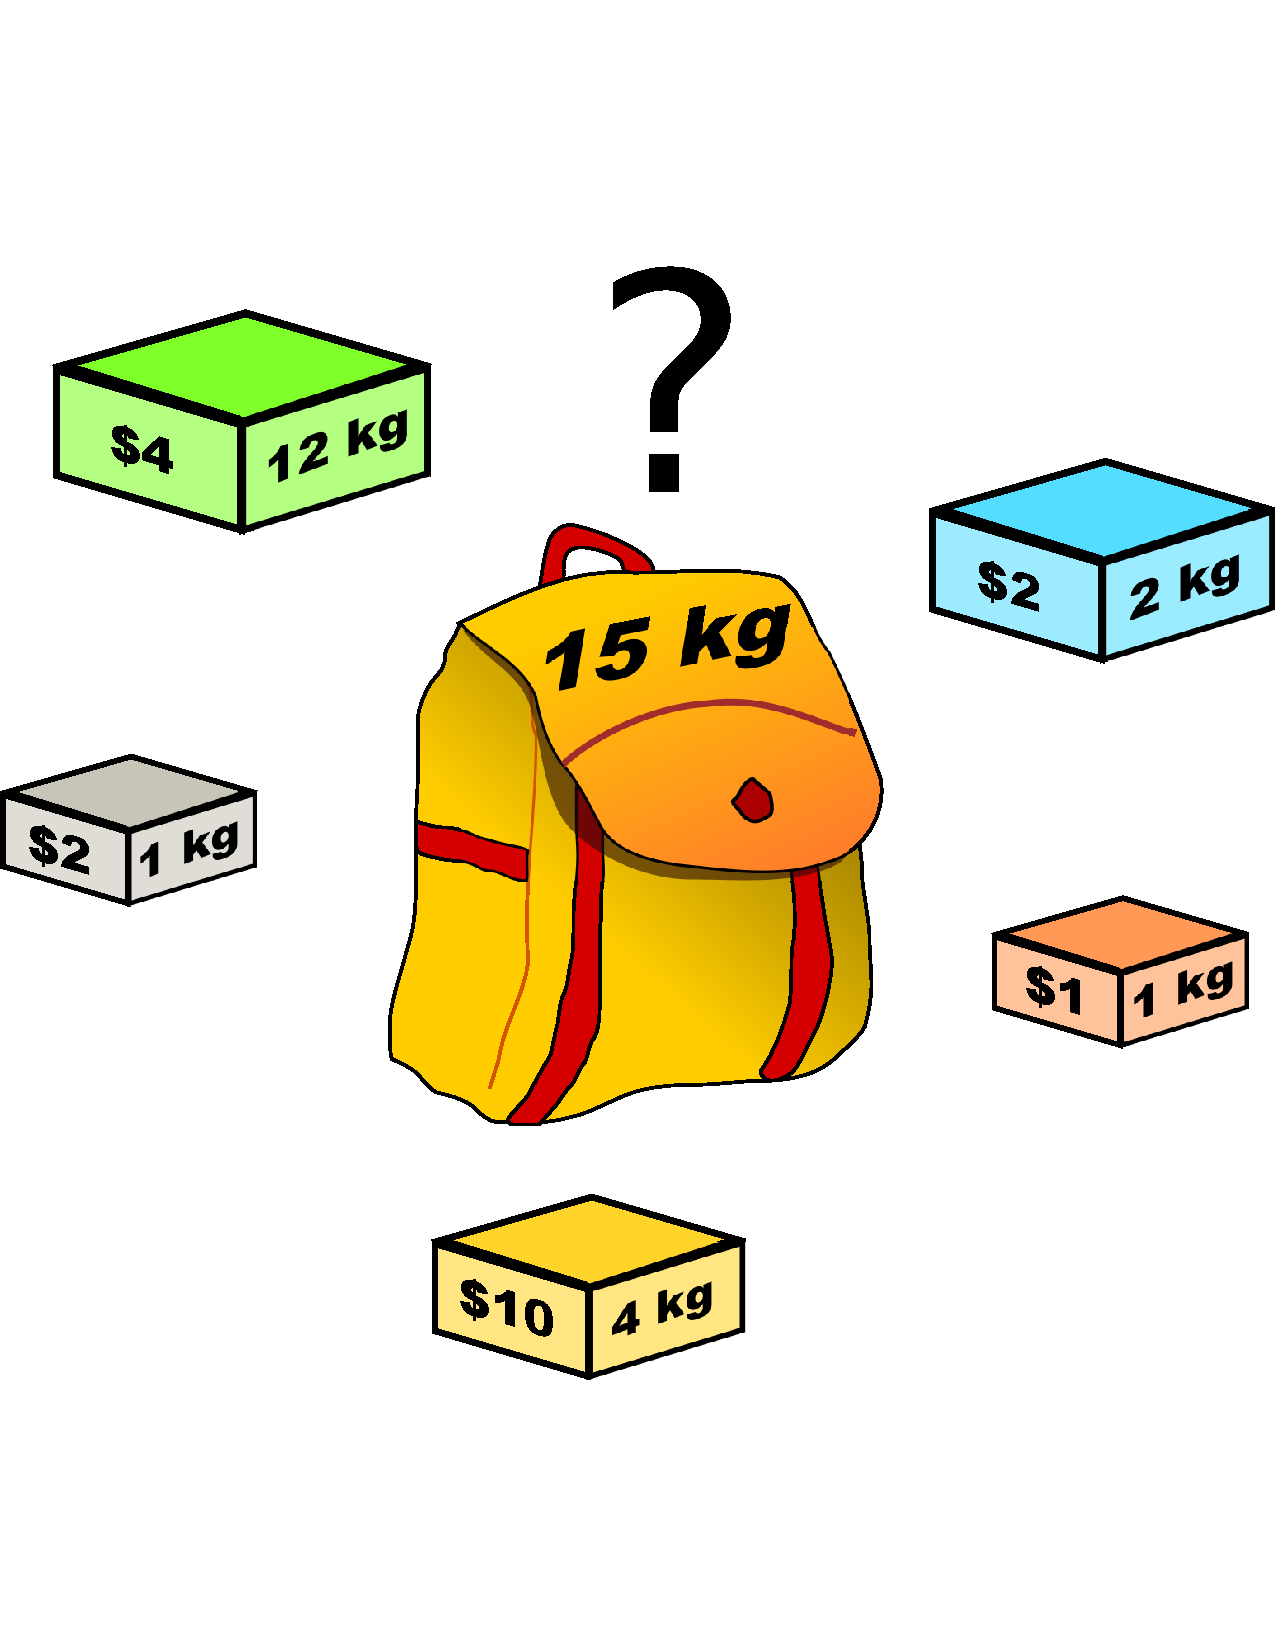
\includegraphics[scale = 0.2]{knapsack}\footnotemark 
%\end{center}
%\label{fig:knapsack}
%\caption{Knapsack Problem: which items should we choose take in the knapsack that maximizes the value while respecting the 15kg weight limit?}
%\end{figure}
%\footnotetext{\url{https://en.wikipedia.org/wiki/Knapsack_problem}}

\begin{examplewithcode}{Knapsack}{https://github.com/open-optimization/open-optimization-or-examples/blob/master/integer-programming/knapsack-problem.ipynb}
\label{example:knapsack}
You have a knapsack (bag) that can only hold W = 15 kgs.  There are 5 items that you could possibly put into your knapsack.  The items (weight, value) are given as:
(12 kg, $\$$4), (2 kg, $\$$2), (1kg, $\$$2), (1kg, $\$$1), (4kg, $\$$10).  Which items should you take to maximize your value in the knapsack? See \autoref{fig:wiki/File/knapsack}.\\

\noindent \textbf{Variables:}
\begin{itemize}
\item let $x_i = 0$ if item $i$ is in the bag
\item let $x_i = 1$ if item $i$ is not in the bag
\end{itemize}
\textbf{Model:}
\begin{align}
\max  \  \ &4 x_1 + 2 x_2 + 2 x_3 + 1 x_4 + 10 x_5 \tag{Total value}\\
\text{ s.t. }\ \ &  12 x_1 + 2 x_2 + 1 x_3 + 1 x_4 + 4 x_5 \leq 15 \tag{Capacity bound}\\
& x_i \in \{0,1\} \text{ for } i=1, \dots, 5 \tag{Item taken or not}
\end{align}
\end{examplewithcode}
In the integer case, we typically require the variables to be non-negative integers, hence we use the notation $x \in \Z^n_+$.  This setting reflects the fact that instead of single individual items, you have item types of which you can take as many of each type as you like that meets the constraint.
\begin{general}{Integer Knapsack Problem}{\npcomplete}
Given an non-negative weight vector $a \in \Q^n_+$, a capacity $b \in \Q_+$, and objective coefficients $c \in \Q^n$, 
\begin{equation}
\begin{split}
\max \ \ & c^\top x\\
\text{s.t.}\ \ & a^\top x \leq b\\
& x \in \Z^n_+
\end{split}
\end{equation}
\end{general}
We can also consider an equality constrained version
\begin{general}{Equality Constrained Integer Knapsack Problem}{\nphard}
Given an non-negative weight vector $a \in \Q^n_+$, a capacity $b \in \Q_+$, and objective coefficients $c \in \Q^n$, 
\begin{align}
\max \ \ & c^\top x\\
\text{s.t.}\ \ & a^\top x = b\\
& x \in \Z^n_+
\end{align}
\end{general}
\begin{example}
\label{ex:min-coins}
Using pennies, nickels, dimes, and quarters, how can you minimize the number of coins you need to to make up a sum of $83\cent$? 

\textbf{Variables:}
\begin{itemize}
\item Let $p$ be the number of pennies used
\item Let $n$ be the number of nickels used
\item Let $d$ be the number of dimes used
\item Let $q$ be the number of quarters used
\end{itemize}
\textbf{Model}
\begin{align*}
\min \quad & p + n + d + q & \text{ total number of coins used}\\
\text{ s.t. } \quad & p + 5n + 10d + 25 q = 83 & \text{sums to } 83 \cent\\
& p,d,n,q \in \Z_+ & \text{each is a non-negative integer}
\end{align*}
\end{example}
\section{Capital Budgeting}


% Copywrite Robert Hildeband 2019

The \emph{capital budgeting} problem is a nice generalization of the knapsack problem.   This problem as the same structure as the knapsack problem, except now it has multiple constraints.   We will first describe the problem, give a general model, and then look at an explicit example.

\begin{general}{Capital Budgeting}{}
\label{general:capital-budgeting}
A firm has $n$ projects it could undertake to maximize revenue, but budget limitations require that not all can be completed.
\begin{itemize}
\item Project $j$ expects to produce revenue $c_j$ dollars overall.
\item Project $j$ requires investment of $a_{ij}$ dollars in time period $i$ for $i = 1,\ldots,m$.
\item The capital available to spend in time period $i$ is $b_i$.
\end{itemize}
Which projects should the firm invest in to maximize it's expected return while satisfying it's weekly budget constriaints?
\end{general}

\newpage

We will first provide a general formulation for this problem.

\begin{general}{Capital Budgeting Model}{}
\noindent \textbf{Sets:}
\begin{itemize}
\item Let $I = \{1, \dots, m\}$ be the set of time periods.
\item Let $J = \{1, \dots, n\}$ be the set of possible investments.
\end{itemize}

\noindent \textbf{Parameters:}
\begin{itemize}
\item $c_j$ is the expected revenue of investment $j$ for $j \in J$
\item $b_i$ is the available capital in time period $i$ for $i$ in  $I$
\item $a_{ij}$ is the resources required for invesment $j$ in time period $i$, for $i$ in $I$, for $j$ in $J$.
\end{itemize}

\noindent \textbf{Variables:}
\begin{itemize}
\item let $x_i = 0$ if investment $i$ is chosen
\item let $x_i = 1$ if investment $i$ is not chosen
\end{itemize}
\textbf{Model:}
\begin{align*}
	\max ~~~& \sum_{j = 1}^n c_jx_j \tag{Total Expected Revenue}\\
	s.t. ~~~&\sum_{j = 1}^n a_{ij}x_j\leq b_i, ~~~i = 1,\ldots m  \tag{ Resource constraint week $i$}\\
	& x_j \in \{0,1\} , \ j = 1,\ldots,n
	\end{align*}

\end{general}


\newpage
%\begin{examplewithcode}{Capital Budgeting}{code:capital-budgeting}
%\label{example:capital-budgeting}
Consider the example given in the following table.
	\begin{table}[h]
			\begin{tabular}{|c|c|c|c|}%[<+->]
				\hline
				Project & $\mathbb{E}$[Revenue] & Resources required in week 1 & Resources required in week 2\\\hline
				\rowcolor{gray!10} 1 & 10 & 3 & 4\\
				\hline
				2 & 8 & 1 & 2\\\hline
				\rowcolor{gray!10} 3 & 6 & 2 & 1\\
				\hline
				Resources available & & 5 & 6\\
				\hline
		\end{tabular}
	\end{table}


Given this data, we can setup our problem explicitly as follows

\begin{examplewithcode}{Capital Budgeting}{https://github.com/open-optimization/open-optimization-or-examples/blob/master/integer-programming/capital-budgeting.ipynb}
\noindent \textbf{Sets:}
\begin{itemize}
\item Let $I = \{1,2\}$ be the set of time periods.
\item Let $J = \{1, 2,3\}$ be the set of possible investments.
\end{itemize}

\noindent \textbf{Parameters:}
\begin{itemize}
\item $c_j$ is given in column "$\mathbb{E}$[Revenue]".
\item $b_i$ is given in row "Resources available".
\item $a_{ij}$ given in row $j$, and column for week $i$.
\end{itemize}

\noindent \textbf{Variables:}
\begin{itemize}
\item let $x_i = 0$ if investment $i$ is chosen
\item let $x_i = 1$ if investment $i$ is not chosen
\end{itemize}

The explict model is given by\\
\noindent  \textbf{Model:}
\begin{align*}
	\max\ \ \  & 10x_1+8x_2+6x_3 \tag{Total Expected Revenue}\\
	s.t. \ \ & 
	3x_1+1x_2+2x_3\leq5 \tag{ Resource constraint week 1}\\
	&4x_1+2x_2+1x_3\leq6 \tag{ Resource constraint week 2}\\
&x_j \in \{0,1\},\  j = 1,2,3
\end{align*}

\end{examplewithcode}




\section{Set Covering}
\begin{resource}
\href{https://www.youtube.com/watch?v=cjSeHSjPmsk}{Video! - Michel Belaire (EPFL) explaining set covering problem}
\end{resource}

The \emph{set covering} problem can be used for a wide array of problems.    We will see several examples in this section.

\begin{general}{Set Covering}{\npcomplete}
\label{general:set-covering}
Given a set $V$ with subsets $V_1, \dots, V_l$, determine the smallest subset $S \subseteq V$ such that 
$S \cap V_i \neq \emptyset$ for all $i=1, \dots, l$.

The set cover problem can be modeled as
\begin{equation}
\begin{split}
\min \ \ & \one^\top x\\
\text{s.t.} \ \ & \sum_{v \in V_i} x_v \geq 1 \text{ for all } i =1, \dots, l \\ 
& x_v \in \{0,1\} \text{ for all } v \in V
\end{split}
\end{equation}
where $x_v$ is a 0/1 variable that takes the value $1$ if we include item $j$ in set $S$ and $0$ if we do not include it in the set $S$.  
\end{general}

\begin{resource}
See \href{https://download.aimms.com/aimms/download/manuals/AIMMS3OM_MediaSelection.pdf}{AIMMS - Media Selection} for an example of set covering applied to media selection.
\end{resource}

\todo[inline]{
Add flight crew scheduling example and images.
}

One specific type of set cover problem is the \emph{vertex cover} problem.
\begin{general}{Example: Vertex Cover}{\npcomplete}
Given a graph $G = (V,E)$ of vertices and edges, we want to find a smallest size subset $S \subseteq V$ such that every for every $e = (v,u) \in E$, either $u$ or $v$ is in $S$.   

We can write this as a mathematical program in the form:
\begin{equation}
\begin{split}
\min \ \ & \one^\top x\\
\text{s.t.} \ \ & x_u + x_v \geq 1 \text{ for all } (u,v) \in E \\ 
& x_v \in \{0,1\} \text{ for all } v \in V.
\end{split}
\end{equation}
\end{general}




\begin{examplewithcode}{Set cover: Fire station placement}{https://github.com/open-optimization/open-optimization-or-examples/blob/master/integer-programming/fire-station-covering.ipynb}
\label{example:fire-station}

In the fire station problem, we seek to choose locations for fire stations such that any district either contains a fire station, or neighbors a district that constains a fire station.  Figure~\ref{fig:tikz/Illustration1.pdf} depicts the set of districts and an example placement of locations of fire stations.  How can we minimize the the total number of fire stations that we need?


\noindent \textbf{Sets:}
\begin{itemize}
\item Let $V$ be the set of districts ($V = \{1, \dots, 16\}$)
\item Let $V_i$ be the set of districts that neighbor district $i$ (e.g. $V_1 = \{2,4,5\}$).
\end{itemize}

\noindent \textbf{Variables:}
\begin{itemize}
\item let $x_i = 1$ if district $i$ is chosen to have a fire station.
\item let $x_i = 0$ otherwise.
\end{itemize}
\textbf{Model:}
\begin{align}
\min  \  \ &\sum_{i \in V} x_i \tag{ \# \text{ open fire stations}}\\
\text{ s.t. }\ \ &  x_i + \sum_{j \in V_i} x_j \geq 1 & \forall{i \in V} \tag{Station proximity requirement}\\
& x_i \in \{0,1\} & \text{ for } i\in V  \tag{station either open or closed}
\end{align}
\end{examplewithcode}

\includefiguresource[Layout of districts and possible locations of fire stations.][][h]{tikz/Illustration1.pdf}
\includefiguresource[Set cover representation of fire station problem.  For example, choosing district 16 to have a fire station covers districts 13, 15, and 16.]{tikz/Illustration2.pdf}
\includefiguresource[Graph representation of fire station problem.  Every node is connected to a chosen node by an edge]{tikz/Illustration3.pdf}



%\documentclass[../open-optimization/open-optimization.tex]{subfiles}

%%%%%%%%%
%\begin{document}
%%%%%%%%%

\begin{general}{Set Covering - Matrix description}{\npcomplete}
\label{general:set-covering-alternate}
Given a non-negative matrix $A \in \{0,1\}^{m \times n}$, a non-negative vector, and an objective vector $c \in \R^n$, the set cover problem is
\begin{equation}
\begin{split}
\max \ \ & c^\top x\\
\text{s.t.}. \ \ & Ax \geq \one \\
& x \in \{0,1\}^n.
\end{split}
\end{equation}
\end{general}
\begin{examplewithoutcode}{Vertex Cover with matrix}{code:vertex-cover-matrix}
An alternate way to solve \nameref{ex:vertex-cover} is to define the \emph{adjacency matrix} $A$ of the graph.  The adjacency matrix is a $|E| \times |V|$ matrix with $\{0,1\}$ entries.  The each row corresponds to an edge $e$ and each column corresponds to a node $v$.  For an edge $e = (u,v)$, the corresponding row has a $1$ in columns corresponding to the nodes $u$ and $v$, and a 0 everywhere else.  Hence, there are exactly two 1's per row.  Applying the formulation above in \nameref{general:set-covering-alternate} models the problem.
\end{examplewithoutcode}




%%%%%%%%%
%\end{document}
%%%%%%%%%




\subsection{Covering (Generalizing Set Cover)}
We could also allow for a more general type of set covering where we have non-negative integer variables and a right hand side that has values other than $1$.
\begin{general}{Covering}{\npcomplete}
\label{general:covering}
Given a non-negative matrix $A \in \Z_+^{m \times n}$, a non-negative vector $b \in \Z^m$, and an objective vector $c \in \R^n$, the set cover problem is
\begin{equation}
\begin{split}
\max \ \ & c^\top x\\
\text{s.t.}. \ \ & Ax \geq b \\
& x \in\Z^n_+.
\end{split}
\end{equation}
\end{general}

%\todo[inline]{
% Add Nurse scheduling problem.
%}
%
%\begin{examplewithcode}{Nurse Scheduling}{code:nurse-scheduling}
%Suppose that we have $n$ full-time nurses employed and $p$ part-time nurses employed.  We need to schedule nurses such that, for each day of the week, we have enough nurses on hand to cover all the tasks.  
%
%\todo[inline]{Add complete example}
%\end{examplewithcode}




\section{Assignment Problem}

The \emph{assignment problem} (machine/person to job/task assignment) seeks to assign tasks to machines in a way that is most efficient.   This problem can be thought of as having a set of machines that can complete various tasks (textile machines that can make t-shirts, pants, socks, etc) that require different amounts of time to complete each task, and given a demand, you need to decide how to alloacte your machines to tasks.

Alternatively, you could be an employer with a set of jobs to complete and a list of employees to assign to these jobs.  Each employee has various abilities, and hence, can complete jobs in differing amounts of time.  And each employee's time might cost a different amout.  How should you assign your employees to jobs in order to minimize your total costs?


\begin{general}{Assignment Problem}{}{}
Given $m$ machines and $n$ jobs, find a least cost assignment of jobs to machines. The cost of assigning job $j$ to machine $i$ is $c_{ij}$.
\end{general}

\todo[inline]{
Include picture and example data
}


\begin{examplewithcode}{Machine Assignment}{https://github.com/open-optimization/open-optimization-or-examples/blob/master/integer-programming/assignment-problem.ipynb}
\noindent \textbf{Sets:}
\begin{itemize}
\item Let $I = \{0,1,2,3\}$ set of machines.
\item Let $J = \{0,1, 2,3\}$ be the set of tasks.
\end{itemize}

\noindent \textbf{Parameters:}
\begin{itemize}
\item $c_{ij}$ - the cost of assigning machine $i$ to job $j$
%\item $c_j$ is given in column "$\mathbb{E}$[Revenue]".
%\item $b_i$ is given in row "Resources available".
%\item $a_{ij}$ given in row $j$, and column for week $i$.
\end{itemize}

\noindent \textbf{Variables:}
\begin{itemize}
\item Let 
\begin{equation*}
x_{ij} = \begin{cases}
1 & \text{if machine $i$ assigned to job $j$}\\
0 & \text{otherwise.}
\end{cases}
\end{equation*}
%\item let $x_i = 1$ if investment $i$ is not chosen
\end{itemize}

\noindent  \textbf{Model:}
\begin{align*}
	\min\ \ \  & \sum_{i \in I, j \in J} c_{ij} x_{ij} \tag{Minimize cost}\\
	s.t. \ \ & \sum_{i \in I} x_{ij} = 1 & \text{for all $j \in J$}
	 \tag{All jobs are assigned one machine}\\
	& \sum_{j \in J} x_{ij} = 1 & \text{for all $i\in I$}
	 \tag{All machines are assigned to a job}\\
	 & x_{ij} \in \{0,1\} \forall i \in I, j \in J
	  \end{align*}
\end{examplewithcode}



\section{Facility Location}
\begin{resource}{}{}
\begin{itemize}
\item \href{https://en.wikipedia.org/wiki/Facility_location_problem}{Wikipedia - Facility Location Problem}
\item See \href{https://github.com/Gurobi/modeling-examples/tree/master/facility_location}{GUROBI Modeling Examples - Facility Location}.
\end{itemize}
\end{resource}
The basic model of the facility location problem is to determine where to place your stores or facilities in order to be close to all of your customers and hence reduce the costs transportation to your customers.  Each customer is known to have a certain demand for a product, and each facility has a capacity on how much of that demand it can satisfy.  Furthermore, we need to consider the cost of building the facility in a given location.

This basic framework can be applied in many types of problems and there are a number of variants to this problem.   We will address two variants: the \emph{capacitated facility location problem} and the \emph{uncapacitated facility location problem}.  
%\todo[inline]{
%Add discussion on Facility Location Problems and pictures.
%}



\subsection{Capacitated Facility Location}

\begin{general}{Capacitated Facility Location}{\npcomplete}
Given costs connections $c_{ij}$ and fixed building costs $f_i$, demands $d_j$ and capacities $u_i$, the capacitated facility location problem is 

\noindent \textbf{Sets:}
\begin{itemize}
\item Let $I = \{1,\dots, n\}$ be the set of facilities.
\item Let $J = \{1, \dots, m\}$ be the set of customers.
\end{itemize}

\noindent \textbf{Parameters:}
\begin{itemize}
\item $f_i$ - the cost of opening facility $i$.
\item $c_{ij}$ - the cost of fulfilling the complete demand of customer $j$ from facility $i$.
\item $u_{i}$ - the capacity of facility $i$.
\item $d_{j}$ - the demand by customer $j$.
%\item $c_j$ is given in column "$\mathbb{E}$[Revenue]".
%\item $b_i$ is given in row "Resources available".
%\item $a_{ij}$ given in row $j$, and column for week $i$.
\end{itemize}

\noindent \textbf{Variables:}
\begin{itemize}
\item Let 
\begin{equation*}
x_{i} = \begin{cases}
1 & \text{if we open facility $i$,}\\
0 & \text{otherwise.}
\end{cases}
\end{equation*}
\item Let $y_{ij} \geq 0$ be the fraction of demand of customer $j$ satisfied by facility $i$.
%\item let $x_i = 1$ if investment $i$ is not chosen
\end{itemize}

\noindent  \textbf{Model:}
\begin{align}
\min & \displaystyle\sum_{i=1}^n\sum_{j=1}^mc_{ij}y_{ij}+\sum_{i=1}^nf_ix_i \tag{total cost}\\
\text{s.t.} & \displaystyle\sum_{i=1}^ny_{ij}=1 \text{ for all }j=1,\dots,m \tag{assign demand to facility}\\
& \displaystyle \sum_{j=1}^md_jy_{ij}\leqslant u_ix_i\text{ for all }i=1\dots,n \tag{capacity of facility $i$}\\
&y_{ij}\geqslant0\text{ for all }i=1,\dots,n \text{ and }j=1,\dots,m \tag{nonnegative fraction of demand satisfied}\\
&x_i\in\{0,1\}\text{ for all } i=1,\dots,n \tag{open/not open facility}
\end{align}

\end{general}

\subsection{Uncapacitated Facility Location}

\begin{general}{Uncapacitated Facility Location}{\npcomplete}
Given costs connections $c_{ij}$ and fixed building costs $f_i$, the uncapacitated facility location problem is 
\begin{equation}
\begin{array}{rl}
\min & \displaystyle\sum_{i=1}^n\sum_{j=1}^mc_{ij}z_{ij}+\sum_{i=1}^nf_ix_i \\
\text{s.t.} & \displaystyle\sum_{i=1}^nz_{ij}=1 \text{ for all }j=1,\dots,m \\
& \displaystyle \sum_{j=1}^mz_{ij}\leqslant Mx_i\text{ for all }i=1\dots,n \\
&z_{ij}\in\{0,1\}\text{ for all }i=1,\dots,n \text{ and }j=1,\dots,m\\
&x_i\in\{0,1\}\text{ for all } i=1,\dots,n
\end{array}
\end{equation}
Here $M$ is a large number and can be chosen as $M = m$, but could be refined smaller if more context is known.
\end{general}


\section{Basic Modeling Tricks - Using Binary Variables}
Binary variables can allow you to model many types of constraints.  We discuss here varios logical constraints where we assume that $x_i \in \{0,1\}$ for $i=1, \dots, n$.  We will take the meaning of the variable to be selecting an item.

\begin{enumerate}
 \item If item $i$ is selected, then item $j$ is also selected.
 \begin{equation}
 x_i \leq x_j
 \end{equation}
 \begin{enumerate}
 \item If any of items $1, \dots, i$ are selected, then item $j$ is selected.
 \begin{equation}
 x_1 + x_2 + \dots + x_i \leq i \cdot x_j
 \end{equation}
 \end{enumerate}
 \item If item $j$ is not selected, then item $i$ is not selected.
 \begin{equation}
x_i \leq x_j
 \end{equation}
  \begin{enumerate}
 \item If item $j$ is not selected, then all items $1, \dots, i$ are not selected.
 \begin{equation}
 x_1 + x_2 + \dots + x_i \leq i \cdot x_j
 \end{equation}
 \end{enumerate}
  \item If item $j$ is not selected, then item $i$ is not selected.
 \begin{equation}
x_i \leq x_j
 \end{equation}
\item Either item $i$ is selected or item $j$ is selected, but not both.
 \begin{equation}
 x_i + x_j = 1
 \end{equation}
\item Item $i$ is selected or item $j$ is selected or both.
 \begin{equation}
 x_i + x_j \geq 1
 \end{equation}
\item If item $i$ is selected, then item $j$ is not selected.
 \begin{equation}
x_j \leq (1-x_i)
 \end{equation}

\item At most one of items $i ,j$, and $k$ are selected.
 \begin{equation}
 x_i + x_j + x_k \leq 1
 \end{equation}
\item At most two of items $i,j,$ and $k$ are selected.
 \begin{equation}
 x_i + x_j + x_k \leq 2
 \end{equation}
\item Exactly one of items $i,j,$ and $k$ are selected.
 \begin{equation}
  x_i + x_j + x_k = 1
 \end{equation}
\end{enumerate}

These tricks can be connected to create different function values.  

\begin{example}{Variable takes one of three values}{}
Suppose that the variable $x$ should take one of the three values $\{4, 8, 13\}$. This can be modeled using three binary variables as
\begin{align*}
x=4z_1 +8z_2 +13z_3\\
 z_1 +z_2 +z_3 =1\\
z_i \in \{0, 1\} \text{ for } i = 1, 2,3.
\end{align*}
As a convenient addition, if we want to add the possibility that it takes the value $0$, then we can model this as 
\begin{align*}
x=4z_1 +8z_2 +13z_3\\
 z_1 +z_2 +z_3 \leq 1\\
z_i \in \{0, 1\} \text{ for } i = 1, 2,3.
\end{align*}
\end{example}


We can also model variable increases at different amounts.  \begin{example}{Discount for buying more}{}
Suppose you can choose to buy 1, 2, or 3 units of a product, each with a decreasing cost.  The first unit is \$10, the second is \$5, and the third unit is \$3.
\begin{align*}
x=10z_1 +5z_2 +3z_3\\
 z_1\geq z_2 \geq z_3\\
z_i \in \{0, 1\} \text{ for } i = 1, 2,3.
\end{align*}
Here, $z_i$ represents if we buy the $i$th unit.  The inequality constraints impose that if we buy unit $j$, then we must by all units $i$ with $i < j$.
\end{example}










\section{Network Flow}
\todo[inline]{Fix up this section}
\begin{center}
\href{https://pixabay.com/illustrations/under-construction-construction-sign-2408060/}{
\includegraphics[scale = 0.05]{optimization/figures/under-construction-2408060_1280}}
\end{center}
\subsection{Example - Multicommodity Flow}

\url{https://en.wikipedia.org/wiki/Multi-commodity_flow_problem}
The \textbf{multi-commodity flow problem} is a
\href{flow_network}{network flow} problem with multiple commodities
(flow demands) between different source and sink nodes.

\paragraph{Problem Definition}

Given a flow network \(\,G(V,E)\), where edge \((u,v) \in E\) has
capacity \(\,c(u,v)\). There are \(\,k\) commodities
\(K_1,K_2,\dots,K_k\), defined by \(\,K_i=(s_i,t_i,d_i)\), where
\(\,s_i\) and \(\,t_i\) is the \textbf{source} and \textbf{sink} of
commodity \(\,i\), and \(\,d_i\) is its demand. The variable
\(\,f_i(u,v)\) defines the fraction of flow \(\,i\) along edge
\(\,(u,v)\), where \(\,f_i(u,v) \in [0,1]\) in case the flow can be
split among multiple paths, and \(\,f_i(u,v) \in \{0,1\}\) otherwise
(i.e. "single path routing"). Find an assignment of all flow variables
which satisfies the following four constraints:

\textbf{(1) Link capacity:} The sum of all flows routed over a link does
not exceed its capacity.

\[\forall (u,v)\in E:\,\sum_{i=1}^{k} f_i(u,v)\cdot d_i \leq c(u,v)\]

\textbf{(2) Flow conservation on transit nodes:} The amount of a flow
entering an intermediate node \(u\) is the same that exits the node.

\[\,\sum_{w \in V} f_i(u,w) - \sum_{w \in V} f_i(w,u) = 0 \quad \mathrm{when} \quad u \neq s_i, t_i\]

\textbf{(3) Flow conservation at the source:} A flow must exit its
source node completely.

\[\,\sum_{w \in V} f_i(s_i,w) - \sum_{w \in V} f_i(w,s_i) = 1\]

\textbf{(4) Flow conservation at the destination:} A flow must enter its
sink node completely.

\[\,\sum_{w \in V} f_i(w,t_i) - \sum_{w \in V} f_i(t_i,w) = 1\]

\hypertarget{corresponding-optimization-problems}{%
\subsection{Corresponding optimization
problems}\label{corresponding-optimization-problems}}

\textbf{Load balancing} is the attempt to route flows such that the
utilization \(U(u,v)\) of all links \((u,v)\in E\) is even, where

\[U(u,v)=\frac{\sum_{i=1}^{k} f_i(u,v)\cdot d_i}{c(u,v)}\]

The problem can be solved e.g. by minimizing
\(\sum_{u,v\in V} (U(u,v))^2\). A common linearization of this problem
is the minimization of the maximum utilization \(U_{max}\), where

\[\forall (u,v)\in E:\, U_{max} \geq U(u,v)\]

In the \textbf{minimum cost multi-commodity flow problem}, there is a
cost \(a(u,v) \cdot f(u,v)\) for sending a flow on \(\,(u,v)\). You then
need to minimize

\[\sum_{(u,v) \in E} \left( a(u,v) \sum_{i=1}^{k} f_i(u,v) \right)\]

In the \textbf{maximum multi-commodity flow problem}, the demand of each
commodity is not fixed, and the total throughput is maximized by
maximizing the sum of all demands \(\sum_{i=1}^{k} d_i\)

\hypertarget{relation-to-other-problems}{%
\subsection{Relation to other
problems}\label{relation-to-other-problems}}

The minimum cost variant of the multi-commodity flow problem is a
generalization of the \href{minimum_cost_flow_problem}{minimum cost flow
problem} (in which there is merely one source \(s\) and one sink \(t\).
Variants of the \href{circulation_problem}{circulation problem} are
generalizations of all flow problems. That is, any flow problem can be
viewed as a particular circulation problem.\footnote{}

\hypertarget{usage}{%
\subsection{Usage}\label{usage}}

\href{Routing_and_wavelength_assignment}{Routing and wavelength
assignment} (RWA) in \href{optical_burst_switching}{optical burst
switching} of \href{SONET}{Optical Network} would be approached via
multi-commodity flow formulas.


\section{Transportation Problem}
\todo[inline]{
Add discussion of transportation problem and picture.
}

\href{https://www.youtube.com/watch?v=Jr7LI-sUEmo}{Youtube! - TRANSPORTATION PROBLEM with PuLP in PYTHON}

\href{https://nbviewer.jupyter.org/github/Pyomo/PyomoGallery/blob/master/transport/transport.ipynb}{Notebook: Solution with Pyomo}

\section{Jobshop Scheduling: Makespan Minimization}
\todo[inline]{
 Add discussion of some makespan minimization problems.
}

\href{https://en.wikipedia.org/wiki/Job_shop_scheduling}{Wikipedia: Jobshop Scheduling}
$$
x_{ij} = \text{ start time of job $j$ on machine $i$}.
$$

$$
y_{ijk} = \begin{cases} 1, & \text{if job } j \text{ precedes job } k \text{ on machine } i \text{,}\\ & i \in I \text{, } j, k  \in J \text{, } j \neq k \\ 0, & \text{otherwise} \end{cases}
$$



\begin{align}\textrm{min: }  &  \\
               & C \\
\textrm{s.t.: } &  \\
               x_{o^{j}_{r}j} &  \geq x_{o^{j}_{r-1}j} +p_{o^{j}_{r-1}j} \,\,\, \forall r \in \{2,..,m\}, j \in {J} \\
                   x_{ij}     & \geq x_{ik} + p_{ik} - M \cdot y_{ijk} \,\,\, \forall j,k \in {J}, j \neq k, i \in {M} \\
                   x_{ik}     & \geq x_{ij} + p_{ij} - M \cdot (1-y_{ijk}) \,\,\, \forall j,k \in {J}, j \neq k,i \in {I} \\
                   C          & \geq x_{o^{j}_{m}j} + p_{o^{j}_{m}j} \,\,\, \forall j \in {J} \\
                  x_{ij}      & \geq 0 \,\,\, \forall i \in {J}, i \in {I} \\
                  y_{ijk}     & \in \{0,1\} \,\,\, \forall j,k \in {J}, i \in {I} \\
                  C & \geq 0
              \end{align}



\section{Quadratic Assignment Problem (QAP)}
\begin{resource}{}{}
\begin{itemize}
\item \href{https://ieeexplore-ieee-org.ezproxy.lib.vt.edu/stamp/stamp.jsp?tp=&arnumber=7170278}{An applied case of quadratic assignment problem in hospital department layout}
\item See \href{https://www.semanticscholar.org/paper/Quadratic-Assignment-Problem%3A-A-survey-and-Shawky-Metwally/247b45613d6d3b6961fdad44f9e7fefb70fd3e82}{Quadratic Assignment Problem: A survey and Applications}.
\end{itemize}
\end{resource}
The quadratic assignment problem must choose the assignment of $n$ facilities to $n$ locations.  Each facility sends some flow to each other facility, and there is a distance to consider between locations.   
The objective is to minimize to distance times the flow of the assignment.


\textbf{Example:  Hospital Layout}
On any given day in the hospital, there will be patients that move from various locations in the hospital to various other locations in the hospital.  For example, patients move from the operating room to a recovery room, or from the emergency room to the operating room, etc.

We would like to chose the locations of these places in the hospital to minimize the amount of total distance traveled by all the patients. 






\begin{general}{Quadratic Assignment Problem}{\npcomplete}
Given flow $f_{ij}$  connections $c_{ij}$ and fixed building costs $f_i$, demands $d_j$ and capacities $u_i$, the capacitated facility location problem is 

\noindent \textbf{Sets:}
\begin{itemize}
\item Let $I = \{1,\dots, n\}$ be the set of facilities.
\item Let $K = \{1, \dots, n\}$ be the set of locations.
\end{itemize}

\noindent \textbf{Parameters:}
\begin{itemize}
\item $f_{ij}$ - flow from facility $i$ to facility $j$.
\item $d_{kl}$ - distance from location $k$ to location $l$.
\item $c_{ik}$ - cost to setup facility $i$ at location $k$.
\end{itemize}

\noindent \textbf{Variables:}
\begin{itemize}
\item Let 
\begin{equation*}
x_{ik} = \begin{cases}
1 & \text{if we place facility $i$ in location $k$,}\\
0 & \text{otherwise.}
\end{cases}
\end{equation*}
\end{itemize}

\noindent  \textbf{Model:}
\begin{align}
\min & \displaystyle\sum_{i=1}^n\sum_{j=1}^n \sum_{k=1}^n \sum_{l = 1}^n f_{ij}d_{kl}x_{ik}x_{jl} + \sum_{i=1}^n \sum_{k = 1}^n c_{ik} x_{ik} \tag{total cost}\\
\text{s.t.} & \displaystyle\sum_{i=1}^n x_{ik}=1 \text{ for all }k=1,\dots,n \tag{assign facility to location $k$}\\
& \displaystyle \sum_{k=1}^n x_{ik}=1 \text{ for all }i=1\dots,n \tag{assign one location to facility $i$}\\
&x_{ik}\in\{0,1\}\text{ for all } i=1,\dots,n, \text{ and } k = 1, \dots, n \tag{binary decisions}
\end{align}
\end{general}

\section{Genaralized Assignment Problem (GAP)}
\todo[inline]{Fix up this section}
\url{https://en.wikipedia.org/wiki/Generalized_assignment_problem}
In \href{applied_mathematics}{applied mathematics}, the maximum
\textbf{generalized assignment problem} is a problem in
\href{combinatorial_optimization}{combinatorial optimization}. This
problem is a \url{generalization} of the
\href{assignment_problem}{assignment problem} in which both tasks and
\href{Agent-based_model}{agents} have a size. Moreover, the size of each
task might vary from one agent to the other.

This problem in its most general form is as follows: There are a number
of agents and a number of tasks. Any agent can be assigned to perform
any task, incurring some cost and profit that may vary depending on the
agent-task assignment. Moreover, each agent has a budget and the sum of
the costs of tasks assigned to it cannot exceed this budget. It is
required to find an assignment in which all agents do not exceed their
budget and total profit of the assignment is maximized.

\hypertarget{in-special-cases}{%
\subsection{In special cases}\label{in-special-cases}}

In the special case in which all the agents' budgets and all tasks'
costs are equal to 1, this problem reduces to the
\href{assignment_problem}{assignment problem}. When the costs and
profits of all tasks do not vary between different agents, this problem
reduces to the multiple knapsack problem. If there is a single agent,
then, this problem reduces to the \href{knapsack_problem}{knapsack
problem}.

\hypertarget{explanation-of-definition}{%
\subsection{Explanation of definition}\label{explanation-of-definition}}

In the following, we have \emph{n} kinds of items, \(a_1\) through
\(a_n\) and \emph{m} kinds of bins \(b_1\) through \(b_m\). Each bin
\(b_i\) is associated with a budget \(t_i\). For a bin \(b_i\), each
item \(a_j\) has a profit \(p_{ij}\) and a weight \(w_{ij}\). A solution
is an assignment from items to bins. A feasible solution is a solution
in which for each bin \(b_i\) the total weight of assigned items is at
most \(t_i\). The solution's profit is the sum of profits for each
item-bin assignment. The goal is to find a maximum profit feasible
solution.

Mathematically the generalized assignment problem can be formulated as
an \href{Integer_programming}{integer program}:
\begin{align} \text{maximize } &
\sum_{i=1}^m\sum_{j=1}^n
p_{ij} x_{ij}. \\
\text{subject to } & \sum_{j=1}^n
w_{ij} x_{ij} \le t_i & & i=1,
\ldots, m; \\ &
\sum_{i=1}^m x_{ij} = 1 & & j=1,
\ldots, n; \\ & x_{ij}
\in \{0,1\} & & i=1,
\ldots, m, \quad j=1,
\ldots, n; \end{align}

%\hypertarget{complexity}{%
%\subsection{Complexity}\label{complexity}}
%
%The generalized assignment problem is \url{NP-hard},\footnote{.}
%However, there are linear-programming relaxations which give a
%\((1 - 1/e)\)-approximation.\footnote{}
%
%\hypertarget{greedy-approximation-algorithm}{%
%\subsection{Greedy approximation
%algorithm}\label{greedy-approximation-algorithm}}
%
%There is a family of algorithms for solving the GAP by using a
%combinatorial translation of any algorithm for the knapsack problem into
%an approximation algorithm for the GAP.\footnote{}
%
%Using any \(\alpha\)-approximation algorithm ALG for the
%\href{knapsack_problem}{knapsack problem}, it is possible to construct a
%(\(\alpha + 1\))-approximation for the generalized assignment problem in
%a greedy manner using a residual profit concept. The algorithm
%constructs a schedule in iterations, where during iteration \(j\) a
%tentative selection of items to bin \(b_j\) is selected. The selection
%for bin \(b_j\) might change as items might be reselected in a later
%iteration for other bins. The residual profit of an item \(x_i\) for bin
%\(b_j\) is \(p_{ij}\) if \(x_i\) is not selected for any other bin or
%\(p_{ij}\) -- \(p_{ik}\) if \(x_i\) is selected for bin \(b_k\).
%
%Formally: We use a vector \(T\) to indicate the tentative schedule
%during the algorithm. Specifically, \(T[i]=j\) means the item \(x_i\) is
%scheduled on bin \(b_j\) and \(T[i]=-1\) means that item \(x_i\) is not
%scheduled. The residual profit in iteration \(j\) is denoted by \(P_j\),
%where \(P_j[i]=p_{ij}\) if item \(x_i\) is not scheduled (i.e.
%\(T[i]=-1\)) and \(P_j[i]=p_{ij}-p_{ik}\) if item \(x_i\) is scheduled
%on bin \(b_k\) (i.e. \(T[i]=k\)).
%
%Formally:
%
%\begin{description}
%\tightlist
%\item[]
%Set \(T[i]=-1 \text{ for } i = 1\ldots n\)
%
%For \(j=1,\ldots,m\) do:
%
%\begin{description}
%\tightlist
%\item[]
%Call ALG to find a solution to bin \(b_j\) using the residual profit
%function \(P_j\). Denote the selected items by \(S_j\).
%
%Update \(T\) using \(S_j\), i.e., \(T[i]=j\) for all \(i \in S_j\).
%\end{description}
%\end{description}
%
%\hypertarget{see-also}{%
%\subsection{See also}\label{see-also}}
%
%\begin{itemize}
%\tightlist
%\item
%  \href{Assignment_problem}{Assignment problem}
%\end{itemize}
%
%\hypertarget{references}{%
%\subsection{References}\label{references}}
%
%\hypertarget{further-reading}{%
%\subsection{Further reading}\label{further-reading}}
%
%\hypertarget{external-links}{%
%\subsection{External links}\label{external-links}}
%
%\href{Category:NP-complete_problems}{Category:NP-complete problems}
%\href{Category:Combinatorial_optimization}{Category:Combinatorial
%optimization}




\section{Other examples}
\begin{itemize}
\item \href{https://www.juliaopt.org/notebooks/JuMP-Sudoku.html}{Sudoku}
\item \href{https://download.aimms.com/aimms/download/manuals/AIMMS3OM_EmployeeTraining.pdf}{AIMMS - Employee Training}

\item \href{https://download.aimms.com/aimms/download/manuals/AIMMS3OM_MediaSelection.pdf}{AIMMS - Media Selection}

\item \href{https://download.aimms.com/aimms/download/manuals/AIMMS3OM_Diet.pdf}{AIMMS - Diet Problem}

\item \href{https://download.aimms.com/aimms/download/manuals/AIMMS3OM_FarmPlanning.pdf}{AIMMS - Farm Planning Problem}

\item \href{https://download.aimms.com/aimms/download/manuals/AIMMS3OM_Pooling.pdf}{AIMMS - Pooling Probem}

\item \href{https://www.informs.org/Impact}{INFORMS - Impact}
\item \href{https://www.informs.org/Impact/O.R.-Analytics-Success-Stories/Optimized-school-bus-routing-helps-school-districts-design-better-policies}{INFORMS - Success Story - Bus Routing}
\end{itemize}
\section{Modeling Tricks}
In this section, we describe ways to model a variety of constraints that commonly appear in practice.  The goal is changing constraints described in words to constraints defined by math.
\subsection{Either Or Constraints}
\emph{``At least one of these constraints holds"} is what we would like to model.  Equivalently, we can phrase this as an \emph{inclusive or} constraint.  
\begin{general}{Either Or}{}{}

\begin{equation}
\text{Either} \ \ \ a^\top x \leq b\ \  \text{  or  } \ \  c^\top x \leq d \ \ \text{holds} 
\end{equation}
can be modeled as 
\begin{equation}
\begin{split}
a^\top x - b &\leq M_1 \delta\\
c^\top x - d &\leq M_2 (1-\delta)\\
\delta &\in \{0,1\},
\end{split}
\end{equation}
where $M_1$ is an upper bound on $a^\top x - b$ and $M_2$ is an upper bound on $c^\top x - d$.
\end{general}

\begin{example}{}{}
Either $2$ buses or $10$ cars are needed shuttle students to the football game.  
\begin{itemize}
\item Let $x$ be the number of buses we have and 
\item let $y$ be the number of cars that we have.  
\end{itemize}
Suppose that there are at most $M_1 = 5$ buses that could be rented an at most $M_2 = 20$ cars that could be available.

This constraint can be modeled as 
\begin{equation}
\begin{split}
x - 2 &\leq 5\delta\\
y - 10 &\leq 20 (1-\delta)\\
\delta &\in \{0,1\},
\end{split}
\end{equation}
\end{example}
\subsection{If then implications}

If then implications are extremely useful in models.  
For instance, if we have more than 5 passengers, then we need to take two cars.   Most if then statements can be modeled with by a constraint and an on/off flag.  For example
\begin{equation}
\text{ If } \ \ \   \delta = 1 \text{, then  } \ \ \ a^\top x \leq b.
\end{equation}
By letting $M$ be an upper bound on the quantity $a^\top x - b$, we can model this condition as 
\begin{equation}
\begin{split}
a^\top x - b& \leq M(1-\delta)\\
\delta & \in \{0,1\}
\end{split}
\end{equation}
On the other hand, if we want to model the reverse implication, we have to be slightly more careful.  We let $m$ be a lower bound on the quantity $a^\top x - b$ and we let $\epsilon$ be a tiny number that is an error bound in verifying if an inequality is violated.  \textbf{If the data $a,b$ are integer and $x$ is an integer, then we can take $\epsilon = 1$.}

Now
\begin{equation}
\text{If } \ \ a^\top x \leq b  \ \ \text{then}\ \ \delta = 1
\end{equation}
can be modeled as 
\begin{equation}
a^\top x -b  \geq  \epsilon(1-\delta) + m \delta.
\end{equation}
A simple way to understand this constraint is to consider the \emph{contrapositive} of the if then statement that we want to model.  The contrapositive says that 
\begin{equation}
\text{If $\delta = 0$, then $a^\top x - b > 0$.}
\end{equation}
To show the contrapositive, we set $\delta = 0$.  Then the inequality becomes 
$$
a^\top x - b \geq \epsilon(1-0) + m0 = \epsilon > 0.
$$
Thus, the contrapositive holds.

\textbf{If instead we wanted a direct proof:}

Case 1: Suppose $a^\top x \leq b$.  Then $0 \geq a^\top x - b$, which implies that 
$$
\delta(a^\top x - b) \geq a^\top x - b
$$
Therefore
$$
\delta(a^\top x - b) \geq \epsilon(1-\delta) + m \delta
$$
After rearranging
$$
\delta(a^\top x - b - m) \geq \epsilon(1-\delta)
$$
Since $a^\top x - b - m \geq 0$ and $\epsilon > 0$, the only feasible choice is $\delta = 1$.


Case 2:  Suppose $a^\top x > b$.  Then $a^\top x - b \geq \epsilon$.    Since $a^\top x -b \geq m$, both choices $\delta = 0$ and $\delta = 1$ are feasible.

By the choice of $\epsilon$,  we know that $a^\top x -b > 0$ implies that $a^\top x - b \geq \epsilon$.  



----


Since we don't like strict inequalities, we write the strict inequality as $a^\top x - b \geq \epsilon$ where $\epsilon$ is a small positive number that is a smallest difference between $a^\top x - b$ and $0$ that we would typically observe.  As mentioned above, if $a,b,x$ are all integer, then we can use $\epsilon = 1$.

Now we want an inequality with left hand side $a^\top x - b \geq$ and right hand side to take the value 
\begin{itemize}
\item $\epsilon$ if $\delta = 0$,
\item $m$ if $\delta = 1$.
\end{itemize}
This is accomplished with right hand side $\epsilon (1-\delta) + m\delta$.

Many other combinations of if then statements are summarized in the following table:
\begin{table}
\begin{center}
\begin{tabular}{|c|c|}
\hline
\textbf{Implication} & \textbf{Constraint}\\
\hline
If $\delta = 0$, then $a^\top x \leq b$ & $a^\top x \leq b + M \delta$\\
If $a^\top x \leq b$, then $\delta = 1$ & $a^\top x \geq m \delta + \epsilon(1-\delta)$\\
\hline
\end{tabular}
\end{center}
\caption{Short list: If/then models with a constraint and a binary variable.  Here $M$ and $m$ are upper and lower bounds on $a^\top x - b$ and $\epsilon$ is a small number such that if $a^\top x > b$, then $a^\top x \geq b + \epsilon$.}
\end{table}
These two implications can be used to derive the following longer list of implications.

\begin{table}
\begin{center}
\begin{tabular}{|c|c|}
\hline
\textbf{Implication} & \textbf{Constraint}\\
\hline
If $\delta = 0$, then $a^\top x \leq b$ & $a^\top x \leq b + M \delta$\\
If $\delta = 0$, then $a^\top x \geq b$ & $a^\top x \geq b + m \delta$\\
If $\delta = 1$, then $a^\top x \leq b$ & $a^\top x \leq b + M (1-\delta)$\\
If $\delta = 1$, then $a^\top x \geq b$ & a$^\top x \geq b + m (1-\delta)$\\
If $a^\top x \leq b$, then $\delta = 1$ & $a^\top x \geq b + m \delta + \epsilon(1-\delta)$\\
If $a^\top x \geq b$, then $\delta = 1$ & $a^\top x \leq b + M \delta - \epsilon(1-\delta)$\\
If $a^\top x \leq b$, then $\delta = 0$ & $a^\top x \geq b + m (1-\delta) + \epsilon \delta$\\
If $a^\top x \geq b$, then $\delta = 0$ & $a^\top x \geq b + m (1-\delta) - \epsilon \delta$\\
\hline
\end{tabular}
\end{center}
\caption{Long list: If/then models with a constraint and a binary variable.  Here $M$ and $m$ are upper and lower bounds on $a^\top x - b$ and $\epsilon$ is a small number such that if $a^\top x > b$, then $a^\top x \geq b + \epsilon$.}
\end{table}
Lastly, if you insist on having exact correspondance, that is, "$\delta = 0 $ if and only if $a^\top x \leq b$" you can simply include both constraints for "if $\delta = 0 $, then $a^\top x \leq b$" and if "$a^\top x \leq b$, then $\delta = 0 $".  Although many problems may be phrased in a way that suggests you need "if and only if", it is often not necessary to use both constraints due to the objectives in the problem that naturally prevent one of these from happening.  

For example, if we want to add a binary variable $\delta$ that means
$$
\begin{cases}
\delta = 0 \text{ implies }  a^\top x \leq b\\
\delta = 1  \text{ Otherwise}
\end{cases}
$$
If $\delta = 1$ does not effect the rest of the optimization problem, then adding the constraint regarding $\delta = 1$ is not necessary.  Hence, typically, in this scenario, we only need to add the constraint $a^\top x \leq b + M \delta$.

\subsection{Binary reformulation of integer variables}
If an integer variable has small upper and lower bounds, it can sometimes be advantageous to recast it as a sequence of binary variables - for either modeling, the solver, or both.   Although there are technically many ways to do this, here are the two most common ways.

\begin{general}{Full reformulation}{\textcolor{blue}{$u$ many binary variables}}
\label{general:full-reformulation}
For a non-negative integer variable $x$ with upper bound $u$, modeled as 
\begin{equation}
0 \leq x \leq u, \ \ \ \ x \in \Z,
\end{equation}
this can be reformulated with $u$ binary variables $z_1, \dots, z_u$ as 
\begin{equation}
\begin{split}
x & = \sum_{i=1}^u i z_i = z_1 + 2 z_2 + \dots + u z_u\\
1 & \geq \sum_{i=1}^u z_i = z_1 + z_2 + \dots + z_u\\
z_i & \in \{0,1\} \ \ \text{ for } i=1, \dots, u
\end{split}
\end{equation}
\end{general}
We call this the \emph{full reformulation} because there is a binary variable $z_i$ associated with every value $i$ that $x$ could take.  That is, if $z_3 = 1$, then the second constraint forces $z_i = 0$ for all $i \neq 3$ (that is, $z_3$ is the only non-zero binary variable), and hence by the first constraint, $x = 3$.

\begin{general}{Binary reformulation}{\textcolor{blue}{$O(\log u)$ many binary variables}}
\label{general:log-reformulation}
For a non-negative integer variable $x$ with upper bound $u$, modeled as 
\begin{equation}
0 \leq x \leq u, \ \ \ \ x \in \Z,
\end{equation}
this can be reformulated with $u$ binary variables $z_1, \dots, z_{\log(\lfloor u \rfloor)+ 1}$ as 
\begin{equation}
\begin{split}
x & = \sum_{i=0}^{\log(\lfloor u \rfloor)+ 1}2^i z_i = z_0 + 2 z_1 +  4 z_2 + 8 z_3 + \dots + 2^{\log(\lfloor u \rfloor) + 1} z_{\log(\lfloor u \rfloor)+ 1}\\
z_i & \in \{0,1\} \ \ \text{ for } i=1, \dots, \log(\lfloor u \rfloor)+ 1
\end{split}
\end{equation}
\end{general}
We call this the \emph{log reformulation} because this requires only logarithmically many binary variables in terms of the upper bound $u$.   This reformulation is particularly better than the full reformulation when the upper bound $u$ is a ``larger" number, although we will leave it ambiguous as to how larger a number need to be in order to be described as a ``larger" number. 
\subsection{SOS1 Constraints}
\begin{definition}{Special Ordered Sets of Type 1 (SOS1)}
A Special Ordered Sets of type 1 (SOS1) constraint on a vector indicates that \emph{at most one element of the vector can non-zero}.
\end{definition}
We next give an example of how to use binary variables to model this and then show how much simpler it can be coded using the SOS1 constraint.

\begin{examplewithcode}{SOS1 Constraints}{https://github.com/open-optimization/open-optimization-or-examples/blob/master/nonlinear-programming/Gurobi-SOS-Examples.ipynb}
\label{example:sos1}
Solve the following optimization problem: \[\begin{aligned}
\text{maximize}\quad & 3x_1 + 4x_2 + x_3 + 5x_4 \\
\text{subject to}\quad & 0 \le x_i \le 5 \\
& \text{at most one of the $x_i$ can be nonzero}
\end{aligned}\]
\end{examplewithcode}
\subsection{SOS2 Constraints}
\begin{definition}{Special Ordered Sets of Type 2 (SOS2)}{}
A \emph{Special Ordered Set of Type 2 (SOS2)} constraint on a vector indicates that \emph{at most two elements of the vector can non-zero AND the non-zero elements must appear consecutively}.
\end{definition}
We next give an example of how to use binary variables to model this and then show how much simpler it can be coded using the SOS2 constraint.
\begin{examplewithcode}{SOS2}{https://github.com/open-optimization/open-optimization-or-examples/blob/master/nonlinear-programming/Gurobi-SOS-Examples.ipynb}
\label{example:SOS2}
Solve the following optimization problem: \[\begin{aligned}
\text{maximize}\quad & 3x_1 + 4x_2 + x_3 + 5x_4 \\
\text{subject to}\quad & 0 \le x_i \le 5 \\
& \text{at most two of the $x_i$ can be nonzero} \\
& \text{and the nonzero $x_i$ must be consecutive}
\end{aligned}\]
\end{examplewithcode}

\subsection{Piecewise linear functions with SOS2 constraint}
\begin{examplewithcode}{Piecewise Linear Function}{https://github.com/open-optimization/open-optimization-or-examples/blob/master/nonlinear-programming/Gurobi-SOS-Examples.ipynb}
\label{example:pwl}
Consider the piecewise linear function 
 $c(x)$ given by
$$
c(x) = 
\begin{cases}
25x  & \text{ if } 0 \leq x \leq 5\\
20x + 25 & \text{ if } 5 \leq x \leq 10\\
15x + 75 & \text{ if } 10 \leq x \leq 15
\end{cases}
$$

\includegraphicstatic[scale = 0.35]{pwl-plot.png}

We will use integer programming to describe this function.  We will fix $x = a$ and then the integer program will set the value $y$ to $c(a)$.
\begin{align*}
\min\quad & 0\\
\text{Subject to} \quad & x - 5 z_{2} - 10 z_{3} - 15 z_{4} = 0\\
 & y - 125 z_{2} - 225 z_{3} - 300 z_{4} = 0\\
 & z_{1} + z_{2} + z_{3} + z_{4} = 1\\
 & SOS2: \{z_1, z_2, z_3, z_4\}\\
 & 0 \leq z_{i} \leq 1 \quad\forall i \in \{1,2,3,4\}\\
 & x = a\\
\end{align*}

\end{examplewithcode}

\begin{examplewithcode}{Piecewise Linear Function Application}{code:pwl-application}
\label{example:pwl-application}
Consider the following optimization problem where the objective function includes the term $c(x)$, where $c(x)$ is the piecewise linear function described in \nameref{example:pwl}:
\begin{align}
\max & z = 12x_{11} + 12x_{21} + 14x_{12} + 14x_{22} - c(x)\\
\text{s.t.} & x_{11} + x_{12} \leq x + 5\\
& x_{21} + x_{22} \leq 10\\
& 0.5 x_{11} - 0.5x_{21} \geq 0\\
& 0.4 x_{12} - 0.6 x_{22} \geq 0\\
& x_{ij} \geq 0\\
& 0 \leq x \leq 15
\end{align}

Given the piecewise linear, we can model the whole problem explicitly as a mixed-integer linear program.

 \begin{equation}
 \begin{array}{rrlr}
 \max\quad & 12 X_{1,1} + 12 X_{2,1} + 14 X_{1,2} + 14 X_{2,2} - y\\
\text{Subject to} \quad & x - 5 z_{2} - 10 z_{3} - 15 z_{4} &= 0\\
 & y - 125 z_{2} - 225 z_{3} - 300 z_{4} &= 0\\
 & z_{1} + z_{2} + z_{3} + z_{4} &= 1\\
 & X_{1,1} + X_{1,2} - x &\leq 5\\
 & X_{2,1} + X_{2,2} \leq 10\\
 & 0.5 X_{1,1} - 0.5 X_{2,1} &\geq 0\\
 & 0.4 X_{1,2} - 0.6 X_{2,2} &\geq 0\\
 & SOS2: \{z_1, z_2, z_3, z_4\}\\
 & X_{i,j} &\geq 0 &\quad\forall i \in \{1,2\}, j \in \{1,2\}\\
 & 0 \leq z_{i} &\leq 1 &\quad\forall i \in \{1,2,3,4\}\\
 & 0 \leq x &\leq 15\\
 & y & \text{ free} \\
\end{array}
\end{equation}
\end{examplewithcode}


\subsubsection{SOS2 with binary variables}

{Modeling Piecewise linear function}
{\begin{itemize}
\item Write down pairs of breakpoints and functions values $(a_i, f(a_i))$.
\item Define a binary variable $z_i$ indicating if $x$ is in the interval $[a_i, a_{i+1}]$.
\item Define multipliers $\lambda_i$ such that $x$ is a combination of the $a_i$'s and therefore the output $y = f(x)$ is a combination of the $f(a_i)$'s.
\item Restrict that at most 2 $\lambda_i's$ are non-zero and that those 2 are consecutive.

\end{itemize}

\begin{align*}
\min \ \ & \sum_{i=1}^k \lambda_i f(a_i)\\
\text{s.t.} \ \ &  \sum_{i=1}^k \lambda_i = 1\\
& x = \sum_{i=1}^k \lambda_i a_i\\
& \lambda_1 \leq z_1\\
& \lambda_i \leq z_{i-1} + z_{i}\\
& \ \ \text{ for }  i=2, \dots, k-1,\\
& \lambda_k \leq z_{k-1}\\
& \lambda_i \geq 0, y_i \in \{0,1\}.
\end{align*}

\subsection{Maximizing a minimum}
When the constraints could be general, we will write $x \in X$ to define general constraints.  For instance, we could have $X = \{ x \in \R^n : Ax \leq b\}$ of $X  = \{ x \in \R^n : Ax \leq b, x \in \Z^n\}$ or many other possibilities.  


Consider the problem 

\begin{align*}
\max   \quad & \min \{x_1, \dots, x_n\}\\
\text{ such that } \quad &  x \in X
\end{align*}
Having the minimum on the inside is inconvenient.  To remove this, we just define a new variable $y$ and enforce that $y \leq x_i$ and then we maximize $y$.  Since we are maximizing $y$, it will take the value of the smallest $x_i$.  Thus, we can recast the problem as

\begin{align*}
\max\quad    & y\\
\text{ such that } \quad  & y \leq x_i \ \text{ for }\  i=1, \dots, n \\
&  x \in X
\end{align*}


\subsection{Relaxing (nonlinear) equality constraints}

There are a number of scenarios where the constraints can be relaxed without sacrificing optimal solutions to your problem.   In a similar vein of the maximizing a minimum, if because of the objective we know that certain constraints will be tight at optimal solutions, we can relax the equality to an inequality.   For example, 
\begin{align*}
\max   \quad &x_1 + x_2 +  \dots + x_n\\
\text{ such that } \quad &  x_i = y_i^2 + z_i^2 \text{ for } i=1, \dots, n
\end{align*}






\section{Notes from AIMMS modeling book.}
\begin{itemize}

\item \href{http://inside.mines.edu/~anewman/MIP_practice120212.pdf}{AIMMS - Practical guidelines for solving difficult MILPs}

\item \href{https://download.aimms.com/aimms/download/manuals/AIMMS3OM_LinearProgrammingTricks.pdf}{AIMMS - Linear Programming Tricks}


\item  \href{https://download.aimms.com/aimms/download/manuals/AIMMS3OM_FormulatingOptimizationModels.pdf}{AIMMS - Formulating Optimization Models}


\item \href{https://pdfs.semanticscholar.org/b01f/ad44c20c372fdda95cbfb980c0d37302de07.pdf}{AIMMS - Practical guidelines for solving difficult linear programs}
\end{itemize}
\subsection{Further Topics}
\begin{itemize}
\item \href{https://or.stackexchange.com/questions/1319/best-model-for-precedence-constraints-within-scheduling-problem}{Precedence Constraints}
\end{itemize}

%\end{document}

% Copyright 2020 by Robert Hildebrand
%This work is licensed under a
%Creative Commons Attribution-ShareAlike 4.0 International License (CC BY-SA 4.0)
%See http://creativecommons.org/licenses/by-sa/4.0/

%\documentclass[../open-optimization/open-optimization.tex]{subfiles}
%
%\begin{document}

%\section{Reference guide for modeling and examples}
%\url{https://download.aimms.com/aimms/download/manuals/AIMMS3_OM.pdf}

\section{MIP Solvers and Modeling Tools}

\begin{itemize}
\item AMPL
\item GAMS
\item AIMMS
\item Python-MIP
\item Pyomo
\item PuLP
\item JuMP
\end{itemize}

\begin{itemize}
\item GUROBI
\item CPLEX (IBM)
\item Express
\item SAS
\item Coin-OR (CBC, CLP, IPOPT)
\item SCIP
\end{itemize}








%%

%\end{document}

% Copyright 2020 by Robert Hildebrand
%This work is licensed under a
%Creative Commons Attribution-ShareAlike 4.0 International License (CC BY-SA 4.0)
%See http://creativecommons.org/licenses/by-sa/4.0/


%\documentclass[../open-optimization/open-optimization.tex]{subfiles}
%
%\begin{document}

\chapter{Algorithms and Complexity}
\todoChapter{ 60\% complete. Goal 80\% completion date: August 20\\
Notes: }
\label{sec:complexity}
\begin{outcome}
\begin{enumerate}
\item Describe asymptotic growth of functions using Big-O notation.
\item Analyze algorithms for the asymptotic runtime.
\item Classify problem types with respect to notions of how difficult they are to solve.
\end{enumerate}
\end{outcome}


\begin{resource}
\begin{itemize}
\item \href{http://web.mit.edu/16.070/www/lecture/big_o.pdf}{MIT Lecture Notes - Big O}
\item \href{https://www.youtube.com/watch?v=YX40hbAHx3s}{Youtube! - P versus NP}
\end{itemize}
\end{resource}

How long will an algorithm take to run?   How difficult might it be to solve a certain problem?   Is the knapsack problem easier to solve than the traveling salesman problem?  Or the matching problem?  
How can we compare the difficulty to solve these problems?

 

We will understand these questions through complexity theory.   We will first use "Big-O" notation to simplify asymptotic analysis of the runtime of algorithms and the size of the input data of an algorithm.  

We will then classify problem types as being either easy ( in the class P) or probably very hard (in the class NP Hard).  We will also learn about the problem classes NP, and NP-Complete.  

To begin, watch these videos (\href{https://www.youtube.com/watch?v=aXXWXz5rF64}{Video 1}, \href{https://youtu.be/TZRWRjq2CAg}{Video 2} )about sorting algorithms.  Notice how a different algorithm can produce a much different number of steps needed to solve the problem.  The first video explains bubble sort and quick sort. The second video explains insertion sort, and then described the analysis of the algorithms (how many comparisons they make as the number of balls to sort grows.    Pay attention to this analysis as this is very crucial in this module.



           

This \href{https://youtu.be/__vX2sjlpXU}{video} is a great introduction to the basic idea of Big-O notation.  We will go over the more formal definition.

    

Here are two great videos about P versus NP (\href{https://youtu.be/EHp4FPyajKQ}{Video 1}, \href{https://youtu.be/YX40hbAHx3s}{Video 2}).  
%
%There is one more complexity class that I find fascinating.  This is called the class of "undecidable problems".   These are problems to which there cannot exist an algorithm general to solve them.  Although this class will not be a focus of this course, if you're interested, watch the following videos that explain the "halting problem", the first problem that was proved to be undecidable. 

         


%\includegraphics[scale = 0.5]{enigma}
%
%\includegraphics[scale = 0.5]{enigma-break}
%
%\url{https://en.wikipedia.org/wiki/Alan_Turing}

\section{Big-O Notation}
We begin with some defintions that relate the rate of growth of functions.   The functions we will look at in the next section will describe the runtime of an algorithm.  



\begin{example}{Relations of functions}{}
We want to understand the asymptotic growth of the following functions:
\begin{itemize}
\item $f(n) = n^2 + 5$,
\item $g(n) = n^3 - 10n^2 -10$.
%\item $h(n) = \tfrac{1}{1000}n^3$
%\item $r(n) = n^4$
\end{itemize}

When we discuss \emph{asymptotic growth}, we don't care so much what happens for small values of $n$, and instead, we want know what happens for large values of $n$.

Notice that 
\begin{equation}
\lim_{n \to \infty} \frac{f(n)}{g(n)} = 0.
\end{equation}
This is because as $n$ gets large, $g(n) >> f(n)$.  However, this does not preclude the possibility that $g(n) < f(n)$ for some small values of $n$, (i.e., $n=1,2,3$).

We can, however see that $g(n) > f(n)$ whenever $n \geq N:= 20$ (it is probably true for a smaller value of $n$, but for the sake of the analysis, we don't care).

Thus, we want to say that $g(n)$ grows faster than $f(n)$.

%\noindent \textbf{$f(n), h(n)$}\\
%Notice that $h(n)$ and $f(n)$ bear the same relation as $g(n)$ and $f(n)$, but this time we must take the value $N$ to be much larger to ensure that $h(n) > f(n)$ for all $n \geq N$.
%
%Again though, we notice that $h(n)$ is function that grows faster.
%
%
%\noindent \textbf{$f(n), h(n)$}\\
%
%
%
%
\end{example}

\begin{example}{Asymptotic Technicality}{}
It may be that we consider functions that are not strictly increasing after some point.  For example,
\begin{itemize}
\item $f(n) = \sin(n)(n^2 + 5)$,
\item $g(n) = 10n^2 -10$.
\end{itemize}

Still, we would like to say that $f(n)$ is bounded somehow by $g(n)$.  But!   The limit $\lim_{n \to \infty} \tfrac{f(n)}{g(n)}$ does not exist!

For this, we use the $\lim\sup$ notation.That is, we notice that 
\begin{equation}
\limsup_{n\to \infty} \tfrac{f(n)}{g(n)} < \infty.
\end{equation}
This completely captures our goal here.  However, we will give an alternative definition that allows us to not have to think about the $\limsup$.
\end{example}


\begin{figure}[h]
\begin{center}
\begin{tikzpicture}
    \draw[->]  (0,0)coordinate(O) -- (8,0) node[anchor=north] {$n$};
    \draw[->]  (0,0) -- (0,5);

\draw[domain=0:8,smooth,variable=\x,blue,name path=c1] plot ({\x},{0.5*\x+2*sin(\x r)+1})node[right]{$c\cdot g(n)$};
\draw[domain=0:8,smooth,variable=\x,blue,name path=c0] plot ({\x},{0.3*0.5*\x+0.3*2*sin(\x r)+0.3*1})node[right]{$g(n)$};
\draw[domain=0:8,smooth,variable=\x,red,name path=c2] plot ({\x},{0.2*\x+0.5*sin(\x r)+2})node[right,black]{$f(n)$};
\fill[red,name intersections={of=c1 and c2}]
    (intersection-1) circle (2pt)
    (intersection-2) circle (2pt)
        (intersection-3) circle (2pt) ;

\draw[dashed] (intersection-3) -- (intersection-3|-O) node[below]{$n_0$};
\end{tikzpicture}
\end{center}
\caption{Example of Big-O notation: $f(n) = O(g(n))$.   We see that for all $n \geq n_0$, we have $c \cdot g(n) \geq f(n)$.  }
\end{figure}



\begin{definition}{Big-O}{}
For two functions $f(n)$ and $g(n)$, we say that $f(n) = O(g(n))$ if there exist positive constants $c$ and $n_0$ such that 
\begin{equation}
\label{eq:bigO}
0 \leq f(n) \leq c\, g(n) \ \ \text{ for all } \ \ \ n \geq n_0.
\end{equation}
\end{definition}



%\includefigurestatic[Example of Big O notation: $f(x) \in O(g(x))$ as there exists $c > 0 $ (e.g. $c = 1$) and $x_0$ (e.g. $x_0 = 5$) such that $f(x) \leq cg(x)$ whenever $x \geq x_0$.]{wiki/File/Big-O-notation.png}


%We can also use Big-O to denote a set as
%\begin{multline}
%O(g(n)) := \{ f(n) :\text{ there exist positive constants $c$ and $n_0$ such that}\\ \text{$0 \leq f(n) \leq c\,g(n)$, for all $n \geq n_0$}\}.
%\end{multline}
\begin{example}
\label{ex:bigO}
Consider $f(n) = 5 n^2 + 10n + 7$ and $g(n) = n^2$.  We want to show that $f(n) = O(g(n))$.  

Let's try $c = 22$ and $n_0 = 1$.  We need to show that \autoref{eq:bigO} is satisfied.

Note first that we always have
\begin{enumerate}
\item $n^2 \leq n^2 \ \ \text{ and therefore } \ \ 5n^2 \leq 5n^2$
\end{enumerate}
Note that if $n \geq 1$, then 
\begin{enumerate}
\setcounter{enumi}{1}
\item $n \leq n^2 \ \ \text{ and therefore } \ \ 10n \leq 10 n^2$
\item $1 \leq n^2 \ \ \text{ and therefore } \ \  7 \leq 7 n^2$
\end{enumerate}
Since all inequalities 1,2, and 3 are valid for $n\geq 1$, by adding them, we obtain a new inequality that is also valid for $n \geq 1$, which is
\begin{align}
5n^2 + 10n + 7 &\leq 5n^2 + 10n^2 + 7 n^2 & \text{ for all } n \geq 1,\\
\Rightarrow \ \ \ \  5n^2 + 10n + 7  & \leq 22 n^2 & \text{ for all } n \geq 1.
\end{align}
Hence, we have shown that \autoref{eq:bigO} holds for $c = 22$ and $n_0 = 1$.  Hence $f(n) = O(g(n))$.
\end{example}



Correct uses:
\begin{itemize}
\item $2^n + n^5 + \sin(n) = O(2^n)$
\item $2^n = O(n!)$
\item $n! + 2^n + 5n = O(n!)$
\item $n^2 + n = O(n^3)$
\item $n^2 + n = O(n^2)$
\item $\log(n) = O(n)$
\item $10 \log(n) + 5 = O(n)$
\end{itemize}
Notice that not all examples above give a tight bound on the asymptotic growth.  For instance, $n^2 + n = O(n^3)$ is true, but a tighter bound is $n^2 + n = O(n^2)$.  

In particular, the goal of big O notation is to give an upper bound on the asymptotic growth of a function.  
But we would prefer to give a strong upper bound as opposed to a weak upper bound.
For instance, if you order a package online, you will typically be given a bound on the latest date that it will arrive.  For example, if it will arrive within a week, you might be guaranteed that it will arrive by next Tuesday.  This sounds like a reasonable bound.  But if instead, they tell you it will arrive before 1 year from today, this may not be as useful information.
In the case of big O notation, we would like to give a least upper bound that most simply describes the growth behavior of the function.

In that example,  
$n^2 + n = O(n^2)$, this literally means that 
there is some number $c$ and some value $n_0$ that 
$n^2 + n \leq c n^2$ for all $n \geq n_0$, 
that is, for all values of $n_0$ larger than $n$, the function $c n^2$ dominates $n^2 + n$.  

For example, a valid choice is $c = 2$ and $n_0 = 1$.  Then it is true that 
$n^2 + n \leq 2 n^2$ for all $n \geq 1$.



But it is also true that $n^2 + n = O(n^3)$.  For example, a valid choice is again $c = 2$ and $n_0 = 1$, then 

$n^2 + n \leq 2 n^3$ for all $n \geq 1$.

In this example, $O(n^3)$ is the case where the internet tells you the package will arrive before 1 year from today.    The bound is true, but it is not as useful information as we would like to have.
Let's compare these upper bounds.  
Let $f(n) = n^2 + n$,
 $g(n) = 2n^2$,
$h(n) = 2n^3$.



Then we have
\begin{verbatim}
                n = 10 .         n = 100 .       n = 1000 .      n = .  10000

f(n)            110,         10100,        1001000,            100010000

g(n)           200,         20000,       2000000,              200000000

h(n) .         2000,       2000000,     2000000000,     2000000000000
\end{verbatim}


So, here we see that $g(n)$ and $h(n)$ are both upper bounds on $f(n)$, but the nice part about $g(n)$ is that is growing at a similar rate to $ f(n)$.  In particular, it is always within a factor of 2 of $f(n)$.  

Alternatively, the bound h(n) is true, but it grows so much faster than $f(n)$ that is doesn't give a good idea of the asymptotic growth of $f(n)$.




Some common classes of functions:
\begin{center}
\begin{tabular}{|c|c|}
\hline
$O(1)$ & Constant\\
$O(\log(n))$ & Logarithmic\\
$O(n)$ & Linear\\
$O(n^c)$ (for $c > 1$) & Polynomial\\
$O(c^n)$  (for $c > 1$ & Exponential\\
\hline
\end{tabular}
\end{center}
\begin{center}
\includefigurestatic[][scale = 0.15][h]{time-of-algorithms}
\end{center}
\section{Algorithms - Example with Bubble Sort}
The following definition comes from Merriam-Webster's dictionary.
\begin{definition}{Algorithm}{}
An algorithm is a procedure for solving a mathematical problem in a finite number of steps that frequently involves repetition of an operation; broadly: a step-by-step procedure for solving a problem or accomplishing some end.
\end{definition}
\subsection{Sorting }
\begin{resource}
\begin{itemize}
\item \href{https://en.wikipedia.org/wiki/Bubble_sort}{Wikipedia}
\end{itemize}
\end{resource}

The problem of sorting a list is a simple problem to think about that has many algorithms to consider.  We will describe one such algorithm: Bubble Sort. 

\begin{general}{Sorting Problem}{\polynomial}{}
Given a list of numbers $(x_1, \dots, x_n)$ sort them into increasing order.  
\end{general}

\begin{example}{Sorting Problem}{}
Suppose you have the list of number $(10, 35, 9, 4, 15, 22)$.

The sorted list of numbers is $(4,9,10,15,22,35)$.
\end{example}

What process or algorithm should we use to compute the sorted list?

\begin{general}{Bubble sort algorithm}{}
The \emph{Bubble Sort} algorithm works as follows:
\begin{enumerate}
\item Compare numbers in position 1 and 2.  If numbers are out of order, then swap them.
\item Next, compare numbers in position 2 and 3.  If numbers are out of order, then swap them.
\item Continue this process of comparing subsequent numbers until you get to the end of the list (and compare numbers in position $n-1$ and $n$.

Now the largest number should be in last position!
\item If no swaps had to be made, then the whole list is sorted!
\item Otherwise, if any swaps were needed, then set the last number aside, and start over from the beginning and sort the remaining list.
\end{enumerate}
\end{general}

\begin{examplewithoutcode}{Bubble Sort}{}{}
Let try using Bubble Sort to sort this list.

\textbf{First pass through the list.}\\
Step 1:
$$ 
(\textbf{10, 35}, 9, 4, 15, 22) \ \ \rightarrow \\ 
(\textbf{10, 35}, 9, 4, 15, 22) 
 $$
 Step 2:
$$ 
(10, \textbf{35,9}, 4, 15, 22) \ \ \rightarrow \\ 
(10, \textbf{9, 35}, 9, 4, 15, 22) 
 $$
 Step 3:
$$ 
(10,9,\textbf{35,4}, 4, 15, 22) \ \ \rightarrow \\ 
(10,9,\textbf{4, 35},15, 22) 
 $$
  Step 4:
$$ 
(10,9,4, \textbf{35,15}, 22) \ \ \rightarrow \\ 
(10,9,4,\textbf{15, 35}, 22) 
 $$
 Step 5:
 $$ 
(10,9,4,15, \textbf{35,22}) \ \ \rightarrow \\ 
(10,9,4,15, \textbf{22, 35}) 
 $$
 Now 35 is in the last spot!\\
 
 \textbf{Second pass through the list}\\
  Step 1:
 $$ 
(\textbf{10,9},4,15,22 \  | \  35) \ \ \rightarrow \\ 
(\textbf{9,10},4,15,22 \  | \  35) 
 $$
   Step 2:
 $$ 
(9,\textbf{10,4},15,22\  | \ 35) \ \ \rightarrow \\ 
(9,\textbf{4,10},15,22\  | \ 35) 
 $$
    Step 3:
 $$ 
(9,4,\textbf{10,15},22\  | \ 35) \ \ \rightarrow \\ 
(9,4,\textbf{10,15},22\  | \ 35) 
 $$
     Step 4:
 $$ 
(9,4,10,\textbf{15,22}\  | \ 35) \ \ \rightarrow \\ 
(9,4,10,\textbf{15,22}\  | \ 35) 
 $$
 
 Now 22 is in the correct spot!\\
 
 \textbf{Third pass through the list}\\
 Step 1:
 $$ 
(\textbf{9,4},10,15, \  | \ 22,35) \ \ \rightarrow \\ 
(\textbf{4,9},10,15, \  | \ 22,35)
 $$
  Step 2:
 $$ 
(4,\textbf{9,10},15, \  | \ 22,35) \ \ \rightarrow \\ 
(4,\textbf{9,10},15, \  | \ 22,35)
 $$
  Step 3:
 $$ 
(4,9,\textbf{10,15}, \  | \ 22,35) \ \ \rightarrow \\ 
(4,9,\textbf{10,15}, \  | \ 22,35)
 $$
  \textbf{Fourth pass through the list}\\
 Step 1:
  $$ 
(\textbf{4,9},10, \  | \ 15, 22,35) \ \ \rightarrow \\ 
(\textbf{4,9},10, \  | \ 15, 22,35)
 $$
  Step 2:
  $$ 
(4,\textbf{9,10}, \  | \ 15, 22,35) \ \ \rightarrow \\ 
(4,\textbf{9,10}, \  | \ 15, 22,35)
 $$
 No swaps were necessary!  We must be done!
 
 
 \textbf{How many comparisons were needed?}\\
 \begin{itemize}
 \item  In the first pass, we needed 5 comparisions
 \item  In the second pass, we needed 4 comparisons
 \item In the third pass, we needed 3 comparisons
 \item In the fourth pass, we needed 2 comparisions
 \end{itemize}
 Thus we used
 $$
 5 + 4 + 3 + 2 = 14 
 $$
 comparisons.
 \end{examplewithoutcode}
 
 \begin{examplewithoutcode}{Worst Case Analysis}{}{}

\textbf{What is the worst case number of comparisons?}

For a list of $n$ numbers, the worst case would be 
$$
(n-1) + (n-2) + \dots + 2 + 1.
$$

Notice that we can compute thus sum exactly in a shorter form.   To do so, let's count the number of pairs that we can get to add up to $n$.  Suppose that $n$ is an even number.
\begin{align*}
(n-1) + 1 &= n\\
(n-2) + 2 & = n\\
(n-3) + 3 & = n\\
&\vdots\\
(n/2 + 1) + (n/2 -1) &= n\\
\end{align*}
Then we also have the number $n/2$ left over.

Adding all this up, we have $(n/2 + 1)$ pairst that add up to $n$, plus one $n/2$ left over. 

Hence, the sum is 
$$
n(\tfrac{n}{2}-1) + \tfrac{n}{2} = \frac{n(n-1)}{2}.
$$

Hence, we have proved that 
$$
\sum_{i=1}^{n-1} i = \frac{n(n-1)}{2}.
$$
Since we just care about the Big-O expression, we can upper bound this by $O(n^2)$.

Hence, we will say that 
\end{examplewithoutcode}










\begin{figure}[h]
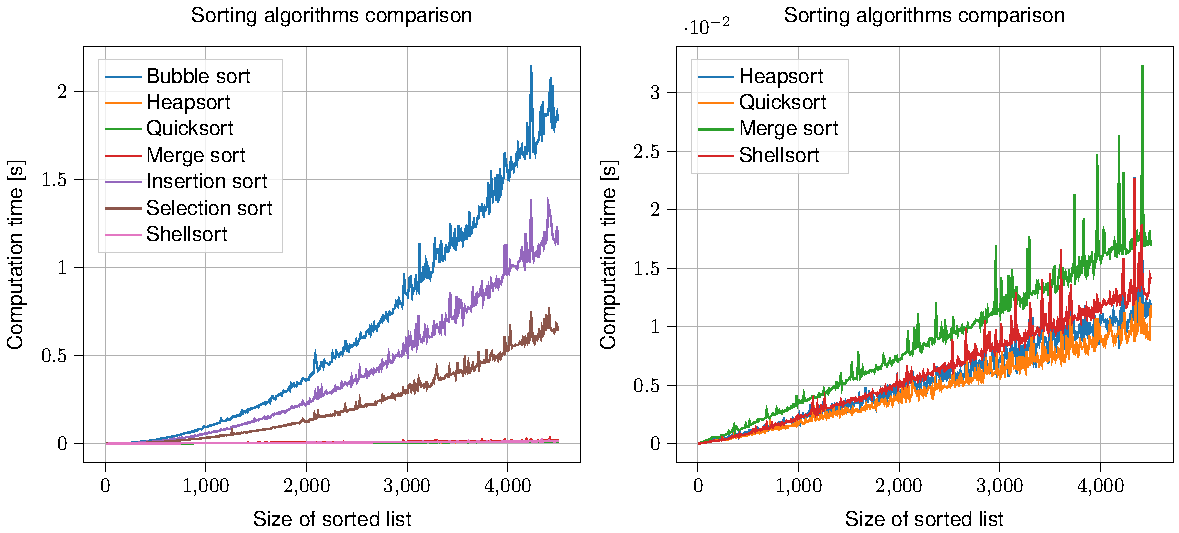
\includegraphics[scale = 0.75]{Sorting_algorithms_comparison}
\caption{Comparison of runtimes of sorting algorithms.}
\end{figure}
%\includefigurestatic[This is a caption.][scale = 0.35][h]{sorting-quadratic}

%\includefigurestatic[][scale = 0.35][h]{sorting-linear}

%\includefigurestatic[][scale = 0.35][h]{bubble-sort-complexity-2}


These can be verified experimentally  as seen in the following plot.  The random case grows quadratically just as the worst case does.  

\includefigurestatic[][scale = 0.35][h]{bubble-sort-computational-example}




There are some other relations that hold:
\begin{theorem}{Summations}{}
\begin{itemize}
\item $
\sum_{i=1}^{n} i = \frac{n(n+1)}{2}.
$
\item $
\sum_{i=1}^{n} i^2 = \frac{n(n+1)(2n+1)}{6}.
$
\item $
\sum_{i=1}^{n} i^3 = \frac{n^2(n+1)^2}{4}.
$
\end{itemize}
There are other formulas, but they get more complicated.  In general, we know that 
\begin{itemize}
\item $\sum_{i=1}^n i^k = O(n^{k+1}).$
\end{itemize}
\end{theorem}



\section{Problem, instance, size}
\subsection{Problem, instance}
\begin{definition}{Problem}{problem}
Is a {\bf generic} question/task that needs to be answered/solved. 

A problem is a ``collection of instances'' (see below).
\end{definition}


A  particular realization of a problem is defined next.

\begin{definition}{Instance}{instance}
An \emph{instance} is a specific case of a problem.  For example, for the problem of sorting, an instance we saw already is $(4,9,10,15,22,35)$.
\end{definition}

\subsection{Format and examples of problems/instances}

A problem is an abstract concept. We will write problems in the following format:
\begin{itemize}
	\item {\bf INPUT:} Generic data/instance.
	\item {\bf OUTPUT:} Question to be answered and/or task to be performed with the data.
\end{itemize}


{\bf Examples of problems/instances:}
	\begin{itemize}
	  \item Typical problems: optimization problems, decision problems, feasibility problems.
		\item LP and IP feasibility, TSP, IP minimization, Maximum cardinality independent set.
	\end{itemize}
	
	\subsection{Size of an instance}
	
The size of an instance is the {\em amount of information} required to represent the instance (in the computer).	Typically, this information is bounded by the quantity of numbers in the problem and the size of the numbers.

\begin{example}{Size of Sorting Problem}{}
Most of the time, we will think of the size of the sorting problem as 
$$
n,
$$
which is the number of numbers taht we need to sort.

However, we should also keep in mind that the size of the numbers is also important.  That is, if the numbers we are asked to sort take up 1 gigabyte of space to write down, then meerly comparing these numbers could take a long time. 

So to be more precise, the size of the problem is
$$
\# \text{ of bits to encode the problem }
$$
which can be upper bounded by 
$$
n \phi_{\max}
$$
where $\phi_{\max}$ is the maximum encoding size of a number given in the data.

For the sake of simplicity, we will typically ignore the size $\phi_{\max}$ in our complexity discussion.  A more rigirous discussion of complexity will be given in later (advanced) parts of the book.
\end{example}


\begin{example}{Size of Matching Problem}{}
The matching problem is presented as a graph $G= (V,E)$ and a set of costs $c_e$ for all $e \in E$.  Thus, the size of the problem can be deceibed as $|V| + |E|$, that is, in terms of the number of nodes and the number of edges in the graph.

\end{example}


\section{Complexity Classes}
In this subsection we will discuss the complexity classes P, NP, NP-Complete, and NP-Hard.  These classes help measure how difficult a problem is.  \textbf{Informally,} these classes can be thought of as 
\begin{itemize}
\item P - the class of efficiently solvable problems
\item NP - the class of efficiently checkable problems
\item NP-Hard - the class of problems that can solve any problem in NP
\item NP-Complete - the class of problems that are in both NP and are NP-Hard.
\end{itemize}
It is not known if $P$ is the same as NP, but it is conjectured that these are very different classes.  This would mean that the NP-Hard problems (and NP-Complete problems) are necessarily much more difficult than the problems in P.  See \refincludefigurestatic[Complexity class possibilities.  Most academics agree that the case $P \neq NP$ is more likely.]{wiki/File/complexity-classes.png}.

We will now discuss these classes more formally.
\subsection{P}
\begin{definition}{P}{}
P is the class of polynomially solvable problems.  P contains all problems for which there exists an algorithm that solves the problem in a run time bounded by a polynomial of input size. That is, $O(n^c)$ for some constant $c$.
\end{definition}

\begin{example}{Sorting}{}
The sorting problem can be solved in $O(n^2)$ time.  Thus, this problem is in $P$
\end{example}

\begin{example}{Complexity Minimum Spanning Tree}{}
The minimum size spanning tree problem is in P.  It can be solved, for instance, by Prim's algorithm, which  by runs in time $O(m \log n)$, where $m$ is the number of edges in the graph and $n$ is the number of nodes in the graph.  
\end{example}
\begin{example}{Complexity Linear Programming}{}
Linear programming is in P.  It can be solved by interior point methods in $O(n^{3.5} \phi)$ where $\phi$ represents the number of binary bits that are required to encode the problem.  These bits describe the matrix $A$, and vectors $c$ and $b$ that define the linear program.
\end{example}
\subsection{NP}
In this section, we will be more specific about the types of problems we want to consider.   In particular, we will consider \emph{decisions problems}.  These are problems where we only request an answer of "yes" or "no".

We can rephrase maximization problems as problems that ask "does there exists a solution with objective value greater than some number?"
\begin{example}{Maximum Matching as a decisions problem}{}
\textbf{Input:} A graph $G = (V,E)$ with weights $w_e$ for $e \in E$ and an objective goal $W$.

\begin{center}
\emph{
Does there exists a matching with objective value greater than $W$?}
\end{center}

\textbf{Output:} Either "yes" or "no".
\end{example}

%\begin{definition}{NP}{}
%\emph{NP} is the class of nondeterministic polynomial problems.  NP contains all problems in which membership can be verified in polynomial time from a \emph{certificate}.
%\end{definition}

We can now define the class of $\NP$.  
	
\begin{definition}{The class $\NP$}{NP2}
Is the set of all decision problems for which a YES answer for a  
particular instance can be {\bf verified} in polytime when provided a \emph{certificate}.

A certificate can be any additional information to help convince someone of a solution.  This should be describable in a compact way (polynomial in the size of the data).  Typically the certificate is simply a feasible solution.
\end{definition}
	
	{\bf Examples:}

\begin{multicols}{2}
\begin{itemize}
\item All problems in $\PP$
\item Integer programming
\item TSP
\item Binary knapsack
\item Maximum independent set
\item Subset sum
\item Partition
\item SAT, $k$-SAT
\item Clique
\end{itemize}
\end{multicols}


Thus, to show that a problem is in NP, you must do the following:
\begin{enumerate}
\item Describe a format for a certificate to the problem.
\item Show that given such a certificate, it is easy to verify the solution to the problem.
\end{enumerate}
\begin{example}{}{}
Integer Linear Programming is in NP.  More explicitly, the feasibility question of
\begin{center}
"Does there exists an integer vector $x$ that satisfies $Ax\leq b$"
\end{center}
is in NP.  

Although it turns out to be difficult to find such an $x$ or even prove that one exists, this problem is in NP for the following reason:  if you are given a particular $x$ and someone claims to you that it is a feasible solution to the problem, then you can easily check if they are correct.  
In this case, the vector $x$ that you were given is called a \emph{certificate}.

Note that it is easy to verify if $x$ is a solution to the problem because you just have to 
\begin{enumerate}
\item Check if $x$ is integer.
\item Use matrix multiplication to check if $Ax \leq b$ holds.
\end{enumerate}
\end{example}
\subsection{Problem Reductions}

We can compare different types of problems by showing that we can use one to solve the other.

A simple example of this is the problem \emph{Integer Programming} and the \emph{Matching Problem}.

Since we can model the \emph{Matching Problem} as an \emph{Integer Program}, then we know that we can solve the \emph{Matching Problem} provided that we can solve \emph{Integer Programs.}
\begin{center}
Matching Problem $\leq$ Integer Programming.
\end{center}

\begin{definition}{Reduction}{}
Given two problems $\mathcal A, \mathcal B$, we say $\mathcal A$ is \emph{reduced to} $\mathcal B$ (and we write $\mathcal A \leq \mathcal B$ when we can assert that if we can solve $\mathcal B$ in polynomial time, then we can also solve $\mathcal A$ in polynomial time.
\end{definition}

\subsection{NP-Hard}
The class of problems that are called \emph{NP-Hard} are those that can be used to solve any other problem in the NP class.  
That is, problem A is NP-Hard provided that for any problem B in NP there is a transformation of problem B that preserves the size of the problem, up to a polynomial factor, into a new problem that problem A can be used to solve.

Here we think of ``if problem A could be solved efficiently, then all problems in NP could be solved efficiently".

More specifically, we assume that we have an oracle for problem A that runs in polynomial time.  An oracle is an algorithm that for the problem that returns the solution of the problem in a time polynomial in the input.   This oracle can be thought of as a magic computer that gives us the answer to the problem.   
Thus, we say that problem A is NP-Complete provided that given an oracle for problem A, one can solve any other problem B in NP in polynomial time.

Note:  These problems are not necessarily in NP.

\subsection{NP-Complete}
The class of problems that are call \emph{NP-Complete} are those which are in NP and also NP-Hard.  

We know of many problems that are NP-Complete.  For example, binary integer programming feasibility is NP-Complete.  One can show that another problem is NP-complete by 
\begin{enumerate}
\item showing that it can be used to solve binary integer programming feasibility,
\item showing that the problem is in NP.
\end{enumerate}

The first problem proven to be NP-Complete is called \emph{3-SAT}~\cite{}.  3-SAT is a special case of the \emph{satisfiability problem}.   In a satisfiability problem, we have variables $X_1, \dots, X_n$ and we want to assign them values as either \true or \false.  The problem is described with \emph{AND} operations, denoted as $\land$,  with \emph{OR} operations, denoted as $\lor$, and with \emph{NOT} operations, denoted as $\neg$.  The \emph{AND} operation $X_1 \land X_2$ returns $\true$ if BOTH $X_1$ and $X_2$ are true.  The \emph{OR} operation $X_1 \lor X_2$ returns $\true$ if AT LEAST ONE OF  $X_1$ and $X_2$ are true.  Lastly, the \emph{NOT} operation $\neg X_1$ returns there opposite of the value of $X_1$.

These can be described in the following table
\begin{align}
\true \land \true = \true\\
\true \land \false = \false\\
\false \land \false = \false\\
\false \land \true = \false
\end{align}

\begin{align}
\true \lor \true = \true\\
\true \lor \false = \true\\
\false \lor \false = \false\\
\false \lor \true = \true
\end{align}

\begin{align}
\neg \true = \false\\
\neg \false = \true
\end{align}

For example, \textbf{Missing code here}
%$$
%\neg \true \lor \false \lor \true = \true \ \ \ \ \true \and \neg \true = \false
%$$
A \emph{logical expression} is a sequence of logical operations on variables $X_1, \dots, X_n$, such that 
\begin{equation}
(X_1 \land \neg X_2 \lor X_3) \land (X_1 \lor \neg X_3) \lor (X_1 \land X_2 \land X_3).
\end{equation}

A \emph{clause} is a logical expression that only contains the operations $\lor$ and $\neg$ and is not nested (with parentheses), such as 
\begin{equation}
X_1 \lor \neg X_2 \lor X_3 \lor \neg X_4.
\end{equation}

A fundamental result about logical expressions is that they can always be reduced to a sequence of clauses that are joined by $\land$ operations, such as 
\begin{equation}
(X_1 \lor \neg X_2 \lor X_3 \lor \neg X_4) \land (X_1 \lor X_2 \lor X_3) \land (X_2 \lor \neg X_3 \lor \neg X_4 \lor X_5).
\end{equation}
The satisfiability problem takes as input a logical expression in this format and asks if there is an assignment of \true  or \false to each variable $X_i$ that makes the expression \true.  The 3-SAT problem is a special case where the clauses have only three variables in them.
 
\begin{general}{3-SAT}{\npcomplete}
Given a logical expression in $n$ variables where each clause has only 3 variables, decide if there is an assignment to the variables that makes the expression \true.
\end{general}


\begin{general}{Binary Integer Programming}{\npcomplete}
Binary Integer Programming can easily be shown to be in NP, since verifying solutions to BIP can be done by checking a linear system of inequalities.  

Furthermore, it can be shown to be NP-Complete since it can be used to solve 3-SAT.  That is, given an oracle for BIP, since 3-SAT can be modeled as a BIP,  the 3-SAT could be solved in oracle-polynomial time.
\end{general}

\section{Problems and Algorithms}
We will discuss the following concepts:
\begin{itemize}
\item Feasible solutions
\item Optimal solutions
\item Approximate solutions
\item Heuristics
\item Exact Algorithms
\item Approximation Algorithms
\item Complexity class relations
\end{itemize}


\subsection{Matching Problem}




\begin{definition}{Matching}{}
Given a graph $G = (V,E)$, a \emph{matching} is a subset $E' \subseteq E$ such that no vertex $v \in V$ is contained in more than one edge in $E'$.  \\
A \emph{perfect matching} is a matching were every vertex is connected to an edges in $E'$.\\
A \emph{maximal matching} is a matching $E'$ such that there is no matching $E''$ that strictly contains it.
\end{definition}


\begin{figure}[H]
\todo[inline]{
INCLUDE PICTURES OF MATCHINGS
%\includegraphics[scale = 0.5]{matchings}\footnotemark
}
\label{fig:matching}
\caption{Two possible matchings.  On the left, we have a perfect matchings (all nodes are matched).  On the right, a feasible matching, but not a perfect matching since not all nodes are matched.}

\end{figure}







\begin{definition}{Maximum Weight Matching}{}
Given a graph $G = (V,E)$, with associated weights $w_e\geq 0$ for all $e \in E$, a \emph{maximum weight matching} is a matching that maximizes the sum of the weights in the matching.
\end{definition}


\includefigurestatic[][scale = 0.5][h]{graph-for-matching-maximal}





%
%\begin{enumerate}
%\item Feasible solution
%\item Greedy Procedure
%\end{enumerate}
%
%\begin{enumerate}
%\item Procedure
%\item Algorithm
%\begin{enumerate}
%\item Heuristic
%\item Approximation
%\item Exact
%\end{enumerate}
%\end{enumerate}
\subsubsection{Greedy Algorithm for Maximal Matching}
The greedy algorithm iteratively adds the edge with largest weight that is feasible to add.  
\begin{general}{Greedy Algorithm for Maximal Matching}{Complexity: $O(|E|\log(|V|))$}
\label{alg:greedy-matching}
\begin{enumerate}
\item Begin with an empty graph $(M = \emptyset)$
\item Label the edges in the graph such that $w(e_1) \geq w(e_2) \geq \dots \geq w(e_m)$
\item For $i=1, \dots, m$\\
\indent  If $M \cup\{e_i\}$ is a valid matching (i.e., no vertex is incident with two edges), then set $M \leftarrow M \cup \{e_i\}$ (i.e., add edge $e_i$ to the graph $M$)
\item Return $M$
\end{enumerate}
\end{general}

\begin{theorem}{Greedy algorithm gives a 2-approximation [\cite{Avis83}]}{}
The greedy algorithm finds a 2-approximation of the maximum weighted matching problem.  That is, $w(M_{greedy}) \geq \tfrac{1}{2} w(M^*)$.
\end{theorem}
%\begin{proof}
%Proof. Let x be the weight of the first edge ( i , j ) that is selected by GREEDY, so that x is in fact an edge of maximum weight in G. Now when (i,j) and all incident edges are deleted, at most two edges of the optimal matching may be removed. Further,thesumoftheirweightscannotexceed2x. Theothern-2ormoreedgesof the optimal matching are candidates for selection at the next iteration of GREEDY. The argument may be repeated for each of the first fniterations of GREEDYII. Since all edge weights are non-negative, the theorem is proved.
%\end{proof}


\subsubsection{Other algorithms to look at}
\begin{enumerate}
\item Improved  Algorithm \cite{DRAKE2003211}
\item Blossom Algorithm \href{https://en.wikipedia.org/wiki/Blossom_algorithm}{Wikipedia}
\end{enumerate}



\subsection{Minimum Spanning Tree}
\begin{definition}{Spanning Tree}{}
Given a graph $G = (V,E)$, a \emph{spanning tree} connected, acyclic subgraph $T$ that contains every node in $V$.
\end{definition}

\includefigurestatic[][scale = 0.=5][h]{spanning-tree}

\begin{definition}{Max weight spanning tree}{}
Given a graph $G = (V,E)$, with associated weights $w_e\geq 0$ for all $e \in E$, a \emph{maximum weight spanning tree} is a spanning tree maximizes the sum of the edge weights.
\end{definition}


\includefigurestatic[][scale = 0.5][h]{spanning-tree-MST}


\begin{lemma}{Edges and Spanning Trees}{}
Let  $G$ be a  connected graph with $n$ vertices.  
\begin{enumerate}
\item $T$ is a spanning tree of $G$ if and only if $T$ has $n-1$ edges and is connected.
\item Any subgraph $S$ of $G$ with more than $n-1$ edges contains a cycle.
\end{enumerate}
\end{lemma}


See Section~\ref{sec:spanning-tree-models} for integer programming formulations of this problem.  
\subsection{Kruskal's algorithm}
\begin{resource}
\href{https://en.wikipedia.org/wiki/Kruskal\%27s_algorithm}{Wikipedia}
\end{resource}
\begin{general}{Kruskal  - for Minimum Spanning tree}{Complexity: $O(|E| \log(|V|)$}
\label{alg:Kruskal}
\begin{enumerate}
\item Begin with an empty tree $(T = \emptyset)$
\item Label the edges in the graph such that $w(e_1) \leq w(e_2) \leq \dots \leq w(e_m)$
\item For $i=1, \dots, m$\\
\indent  If $T \cup\{e_i\}$ is acyclic, then set $T \leftarrow T \cup \{e_i\}$
\item Return $T$
\end{enumerate}
\end{general}


%\begin{general}{Acyclic Graph}{}
%\label{alg:Acyclic}
%\textbf{Input:} An acyclic graph $T$ and an edge $e$
%\textbf{Output:} Either "Yes" - $T \cup \{e\}$ contains a cycle or "No" it does not contain a cycle.
%\begin{enumerate}
%\item Begin with an empty tree $(T = \emptyset)$
%\item Label the edges in the graph such that $w(e_1) \leq w(e_2) \leq \dots \leq w(e_m)$
%\item For $i=1, \dots, m$\\
%\indent  If $T \cup\{e_i\}$ is acyclic, then set $T \leftarrow T \cup \{e_i\}$
%\item Return $T$
%\end{enumerate}
%\end{general}


%\begin{proof}
%
%\end{proof}

\subsubsection{Prim's Algorithm}
\begin{resource}
\begin{itemize}
\item \href{https://en.wikipedia.org/wiki/Prim\%27s_algorithm}{Wikipedia}
\item \href{http://www.texample.net/tikz/examples/prims-algorithm/}{TeXAmple - Figure for min spannig tree}
\end{itemize}
\end{resource}

\subsection{Traveling Salesman Problem}
\begin{resource}
\begin{itemize}
\item 
\end{itemize}
\end{resource}

See Section~\ref{sec:tsp-models} for integer programming formulations of this problem.  Also, hill climbing algorithms for this problem such as 2-Opt, simulated annealing, and tabu search will be discussed in Section~\ref{sec:IP-Heuristics}.

\subsubsection{Nearest Neighbor - Construction Heuristic}
\begin{resource}
\href{https://en.wikipedia.org/wiki/Nearest_neighbour_algorithm}{Wikipedia}
\end{resource}
We will discuss heuristics more later in this book.   For now, present this construction heuristic as a simple algorithmic example.   


Starting from any node, add the edge to the next closest node.  Continue this process.
\begin{general}{Nearest Neighbor}{Complexity: $O(n^2)$}
\label{heuristic:nearestNeighbor}
\begin{enumerate}
\item Start from any node (lets call this node 1) and label this as your current node.
\item Pick the next current node as the one that is closest to the current node that has not yet been visited.
\item Repeat step 2 until all nodes are in the tour.
\end{enumerate}
\end{general}

\subsubsection{Double Spanning Tree - 2-Apx}
We can use a minimum spanning tree algorithm to find a provably okay solution to the TSP, provided certain properties of the graph are satisfied.  

Graphs with nice properties are often easier to handle and typically graphs found in the real world have some nice properties. The \emph{triangle inequality} comes from the idea of a triangle that the sum of the lengths of two sides always are longer than the length of the third side. See \refincludefigurestatic{wiki/File/triangle_inequality.png}


\begin{definition}{Triangle Inequality on a Graph}{}
A complete, weighted graph $G$ (i.e., a graph that has all possible edges and a weight assigned to each edge) satisfies the \emph{triangle inequality} provided that for ever triple of vertices $a,b,c$ and edges $e_{ab}, e_{bc}, e_{ac}$, we have that 
\[
w(e_{ab}) + w(e_{bc}) \geq w(e_{ac}).
\]
\end{definition}



\begin{algorithm}
\algorithmicrequire{A graph $G = (V,E)$ that satisfies the triangle inequality}\\
\algorithmicensure{A tour that is a 2-Apx of the optimal solution}
\caption{Double Spanning Tree}\label{alg:double-spanning-tree}
\begin{algorithmic}[1]
	\State Compute a minimum spanning tree $T$ of $G$.
 	\State Double each edge in the minimum spanning tree (i.e., if edge $e_{ab}$ is in $T$, add edge $e_{ba}$. 
	\State Compute an Eulerian Tour  using these edges.
	\State Return tour that visits vertices in the order the Eulerian Tour visits them, but without repeating any vertices.
	\end{algorithmic}
\end{algorithm}

Let $S$ be the resulting tour and let $S^*$ be an optimal tour.
Since the resulting tour is feasible, it will satisfy 
\[
w(S^*) \leq w(S).
\]
But we also know that the weight of a minimum spanning tree $T$ is less than that of the optimal tour, hence
\[
w(T) \leq w(S^*).
\]
Lastly, due to the triangle inequality we know that 
\[
w(S) \leq 2 w(T),
\]
since replacing any edge in the Eulerian tour with a more direct edge only reduces the total weight.

Putting this together, we have

\[w(S) \leq 2w(T) \leq 2 w(S^*)\]
and hence, $S$ is a 2-approximation of the optimal solution.


\subsubsection{Christofides - Approximation Algorithm - $(3/2)$-Apx}
If we combine algorithms for minimum spanning tree and matching, we can find a better approximation algorithm.  This is given by Christofides.  Again, this is in the case where the graph satisfies the triangle inequality.  See 
\href{https://en.wikipedia.org/wiki/Christofides_algorithm}{Wikipedia - Christofides Algorithm} or \href{https://resources.mpi-inf.mpg.de/conferences/adfocs-15/material/Ola-Lect1.pdf}{Ola Svensson Lecture Slides} for more detail.

%\end{document}

% Copyright 2020 by Robert Hildebrand 
% contributed by Diego Moran
%This work is licensed under a
%Creative Commons Attribution-ShareAlike 4.0 International License (CC BY-SA 4.0)
%See http://creativecommons.org/licenses/by-sa/4.0/

%\documentclass[../open-optimization/open-optimization.tex]{subfiles}
%
%\begin{document}
%\newcommand{\mathup}[1]{#1}
%\newcommand{\NP}{\text{NP}}
%\newcommand{\coNP}{\text{coNP}}

\chapter{Introduction to computational complexity}
\todoChapter{ Move this section to mode advanced version of the book.}

\section{Introduction}

{\bf Motivation:} We want to understand {\em what} is a problem and {\em when} a problem is {\em easy}/{\em hard}.\\

{\bf Our strategy:} An intuitive review of the basic ideas in Computational Complexity theory.\\ 

{\bf Key concepts:}
	\begin{itemize}
		\item Problem types: optimization problems, decision problems, feasibility problems.
		\item Instance (of a problem)
		\item A problem is a collection of instances.
		\item Size of an instance
		\item Algorithm
		\item Running time of an algorithm; worst-case time complexity
		\item Complexity classes: ${\mathup{P}}$ and ${\mathup{NP}}$
\end{itemize}

\section{Problem, instance, size}
\subsection{Problem, instance}
\begin{definition}{Problem}{problem}
Is a {\bf generic} question/task that needs to be answered/solved. 

A problem is a ``collection of instances'' (see below).
\end{definition}


A {\em particular} realization of a problem is define next.

\begin{definition}{Instance}{instance}
Is a specific case of a problem. In other words, we can say ``Instance$\in$Problem''.
\end{definition}

\subsection{Format and examples of problems/instances}

A problem is an abstract concept. We will write problems in the following format:
\begin{itemize}
	\item {\bf INPUT:} Generic data/instance.
	\item {\bf OUTPUT:} Question to be answered and/or task to be performed with the data.
\end{itemize}


{\bf Examples of problems/instances:}
	\begin{itemize}
	  \item Typical problems: optimization problems, decision problems, feasibility problems.
		\item LP and IP feasibility, TSP, IP minimization, Maximum cardinality independent set.
	\end{itemize}
	
	\subsection{Size of an instance}
	
The size of an instance is the {\em amount of information} required to represent the instance (in the computer).	
	
\begin{definition}{Binary size/length}{size}
Is the number of bits that are needed in order to give the problem to a computer.
\end{definition}	
	
{\bf Examples of sizes:}
	\begin{itemize}
		\item Size of an integer/rational number.
		\item Size of a rational matrix.
		\item Size of a graph (node-egde matrix represetation).
	\end{itemize}

\section{Algorithms, running time, Big-O notation}
\subsection{Basics}
\begin{definition}{Algorithm}{algorithm}
List of instructions to solve a problem.
\end{definition}

	
\begin{definition}{Running time of an algorithm}{running-time}
Is the number of steps (as a function of the size) that the algorithm takes in order to solve an instance. 
\end{definition}


	
	

\subsection{Worst-time complexity}	

Given an algorithm $\AA$ to solve a problem $P$, the {\em running time of $\AA$}, as a function of the size $\sigma\in\Z_+$ will be defined as follows:
\begin{itemize}
	\item The (generic) running time will be a function $f:\Z_+\rightarrow\Z_+$.
   \item Given $\sigma$, the function $f$ is defined as follows:
		$$f(\sigma)=\max\{\textup{running time of $\AA$ for instance $z$, where $\size(z)\leq \sigma$}\}.$$
\end{itemize}
	
{\bf Remark:} This is a very conservative/pessimistic measure of running time.	
\subsection{Big-O notation}

A function 	$f:\Z_+\rightarrow\Z_+$ belongs to the class of functions $\textup{O}(g(n))$ (that is, $f\in\textup{O}(g(n))$) if there exists $c>0$, $n_0\in\Z_+$ such that
$$f(n)\leq c g(n),\quad \textup{for all}\ n\geq n_0.$$

We usually say ``$f$ is $\textup{O}(g(n))$'' or ``$f$ is order $\textup{O}(g(n))$''.
	\subsection{Examples} 
\begin{itemize}
  \item Basic examples of Big-O notation: $\textup{O}(1)$, $\textup{O}(n^k)$, $\textup{O}(c^n)$, $\textup{O}(\log(n))$, etc.
	\item An illustration of the fact that the running time depends on the size of the instance: the algorithm for the binary knapsack problem that is $O(nb)$ is not polynomial, since the size of the instance is $\log(b)$.
\end{itemize}	
 




\section{Basics}

\begin{definition}{Polynomial time algorithm}{polytime}
An algorithm is said to be a {\em polynomial time algorithm} if its running time is $\textup{O}(n^k)$ for some $k\geq 1$ (where $n$ representes the size of a generic instance).
\end{definition}

{\bf Remark:} {\em Polynomial time algorithms} are also known as  {\em Polytime algorithms}.

\begin{definition}{Decision problem}{decision-problem} 
A decision problem  is  any problem whose only acceptable answers are either YES or NO (but not both at the same time).
\end{definition}



{\bf Some examples:} feasibility problems, decision version of optimization problems, etc.

\section{Complexity classes}

We will introduced 3 complexity classes (For see at least 495 more classes, please see \url{http://complexityzoo.uwaterloo.ca/Complexity_Zoo}).

\subsection{Polynomial time problems} 
\begin{definition}{The class $\PP$}{PP} 
Is the set of all decision problems for which a YES or NO answer for a  
particular instance can be {\bf obtained} in polytime.
\end{definition}

{\bf Remark:} For a particular problem $P$, there are 3 possibilities: (1) $P\in\PP$, (2) $P\notin\PP$, and $P\ \text{?}\ \PP$ (i.e., we don't know). 

{\bf Examples:}

\begin{multicols}{2}
\begin{itemize}
	\item Shortest path
	\item Max flow
	\item Min cut
	\item Matroid optimization
	\item Matchings
	\item Linear programming
\end{itemize}
\end{multicols}

	\subsection{Non-deterministic polynomial time problems}
	
	\begin{definition}{The class $\NP$}{NP2}
Is the set of all decision problems for which a YES answer for a  
particular instance can be {\bf verified} in polytime.
\end{definition}
	
	{\bf Examples:}

\begin{multicols}{2}
\begin{itemize}
\item All problems in $\PP$
\item Integer programming
\item TSP
\item Binary knapsack
\item Maximum independent set
\item Subset sum
\item Partition
\item SAT, $k$-SAT
\item Clique
\end{itemize}
\end{multicols}
	
	\subsection{Complements of problems in $\NP$}
	\begin{definition}{The class $\NP$}{NP} 
Is the set of all decision problems for which a NO answer for a  
particular instance can be {\bf verified} in polytime.
\end{definition}

	{\bf Examples:}

\begin{multicols}{2}
\begin{itemize}
\item All problems in $\PP$
\item Every ``complement'' of an $\NP$ problem
\item PRIMES
\end{itemize}
\end{multicols}

{\bf Remark}: Actually, $\textup{PRIMES}\in\NP$ (see {\em Pratt's certificates}), even better, it was recently proven that $\textup{PRIMES}\in\PP$ (by Manindra Agrawal, Neeraj Kayal, Nitin Saxena in 2004).

\section{Relationship between the classes}
\subsection{A basic result}
 
\begin{theorem}{}{} The following relationship holds:
 $$\PP\subseteq \NP\cap\coNP.$$
\end{theorem}

\subsection{An \$1,000,000 open question}
 The question ``Is $\PP=\NP$?'' is one of the most important problems in mathematics and computer science. A correct answer is worth 1 Million dollars! Most people believe that $\PP\neq \NP$.

 \section{Comparing problems, Polynomial time reductions}

{\bf Motivation:} We would like to solve problem $P_1$ by efficiently {\em reducing} it to another problem $P_2$ (why? Perhaps we know how to solve $P_2$!!!).

	\begin{definition}{Polynomial time reductions}{reduction}
Let $P_1,P_2$ be decision problems. We say that $P_1$ is {\em polynomially reducible to $P_2$} (denoted $P_1\leq_{\PP}P_2$) if there exists a function
$$f:P_1\rightarrow P_2$$
such that 
\begin{enumerate}
	\item For all $w\in P_1$ the answer to $w$ is YES if and only if the answer to $f(w)$ is YES.
	\item For all $w\in P_1$ $f(w)$ can be computed in polynomial time w.r.t to $\size(w)$. In particular, we must have that $\size(f(w))$ is polynomially bounded by $\size(w)$.
\end{enumerate}
\end{definition}

{\bf Remarks:} \begin{enumerate}
	\item In the above definition ``$f$ efficiently transforms an instance of $P_1$ into an instance of $P_2$''. In particular, if we know how to solve problem $P_2$, then we can solve problem $P_1$.
	\item Therefore, the notation $P_1\leq_{\PP}P_2$ makes sense: we are saying that $P_1$ is ``easier'' to solve than $P_2$, as any algorithm for $P_2$ would work for $P_1$. 
\end{enumerate} 



\section{Comparing problems, Polynomial time reductions}
\subsection{Definition}
{\bf Motivation:} We would like to solve problem $P_1$ by efficiently {\em reducing} it to another problem $P_2$ (why? Perhaps we know how to solve $P_2$!!!).

	\begin{definition}{Polynomial time reductions}{reducible}
Let $P_1,P_2$ be decision problems. We say that $P_1$ is {\em polynomially reducible to $P_2$} (denoted $P_1\leq_{\PP}P_2$) if there exists a function
$$f:P_1\rightarrow P_2$$
such that 
\begin{enumerate}
	\item For all $w\in P_1$ the answer to $w$ is YES if and only if the answer to $f(w)$ is YES.
	\item For all $w\in P_1$ $f(w)$ can be computed in polynomial time w.r.t to $\size(w)$. In particular, we must have that $\size(f(w))$ is polynomially bounded by $\size(w)$.
\end{enumerate}
\end{definition}

{\bf Remarks:} \begin{enumerate}
	\item In the above definition ``$f$ efficiently transforms an instance of $P_1$ into an instance of $P_2$''. In particular, if we know how to solve problem $P_2$, then we can solve problem $P_1$.
	\item Therefore, the notation $P_1\leq_{\PP}P_2$ makes sense: we are saying that $P_1$ is ``easier'' to solve than $P_2$, as any algorithm for $P_2$ would work for $P_1$. 
\end{enumerate} 
\subsection{Basic properties}

\begin{proposition}{}{} Let $P_1,P_2$ be two problems such that $P_1\leq_{\PP}P_2$ and assume that $P_2\in \PP$. Then $P_1\in\PP$.
\end{proposition}

\begin{proposition}{}{} Let $P_1,P_2$ be two problems such that $P_1\leq_{\PP}P_2$ and assume that $P_2\in \NP$. Then $P_1\in\NP$.
\end{proposition}

\begin{proposition}{}{} Let $P_1,P_2,P_3$ be three problems assume that $P_1\leq_{\PP}P_2$ and $P_2\leq_{\PP}P_3$. Then $P_1\leq_{\PP}P_3$.
\end{proposition}

\section{$\NP$-Completeness}
\subsection{The basics}
\begin{definition}{$\NP$-Completeness}{NP-complete}
A decision problem $P$ is said to be $\NP$-complete if:
\begin{enumerate}
	\item $P\in \NP$
	\item $Q\leq_{\PP}P$ for all $Q\in\NP$ (that is, every problem $Q$ in $\NP$ can be polynomially reduced to $P$). 
\end{enumerate}
\end{definition}

\begin{proposition}{}{} If $P$ is $\NP$-complete and $P\in\PP$ then $\PP=\NP$.
\end{proposition}
\subsection{Do $\NP$-complete problems  exist?}
\begin{theorem}{S. Cook, 1971}{sat-complete}
SAT is $\NP$-complete.  
\end{theorem}
\section{$\NP$-Hardness}
\begin{definition}{$\NP$-Completeness}{NPcomplete}
A problem $P$ is said to be $\NP$-hard if there exists a $\NP$-complete decision problem that can be reduced to it. 
\end{definition}

{\bf Remarks:}
\begin{itemize}
	\item $\NP$-complete problems are $\NP$-hard.
	\item Problems in $\NP$-hard not need to be decision problems.
	\item Optimization versions of $\NP$-complete decision problems are $\NP$-hard.
	\item If $P$ is $\NP$-hard and $P\in\PP$ then $\PP=\NP$.
\end{itemize}

\section{Exercises}

\begin{enumerate}
\item Let $P,Q$ be decision problems such that every instance of $Q$ is an instance of $P$ {\color{black}(that is $\{\text{instances in $Q$}\}\subseteq \{\text{instances in $P$}\}$)}.
\begin{enumerate}
	\item Give an example of $P,Q$ such that $Q\in \PP$ and $P\in \NP-\text{complete}$. 
		\item Give an example of $P,Q$ such that $Q,P\in \NP-\text{complete}$. 
\end{enumerate} 

{\bf Note:} You must prove that your problem belongs to the corresponding class unless we have proved or sketched the proof of that fact in class.\\ 

{\bf \Large Solution:}\\

\begin{enumerate}
	\item \begin{itemize}
		\item Let $P$ be the {\em Knapsack problem}. Then $P$ is $\NP$-complete (see Problem 5).
		\item Let $Q$ be the special case of the {\em Knapsack problem} where all weights are 1, that is, $a_1,\dots,a_n=1$. The following algorithm decides this special case:
		
			{\tt ALGORITHM:}
			
			\begin{itemize}
				\item[1.] List the objects $1,\dots,n$ in decreasing order according to $c_1,\dots,c_n$.
				\item[2.] Select the first $b$ objects from that list. Call this set $S$.
				\item[3.] If $\sum_{i\in S}c_i\leq k$, then  the output of the algorithm is YES. Else, the output is NO. 
			\end{itemize}
			
			Clearly, this algorithm is correct and runs in polynomial time w.r.t. to the instance. Hence, $Q\in\PP$.
			
	\end{itemize}
	\item \begin{itemize}
		\item Let $P$ be {\em SAT}.
		\item Let $Q$ be {\em 3-SAT}.
	\end{itemize}
	
	We showed in class that both $P$ and $Q$ are  $\NP$-complete problems.
	
\end{enumerate}
\newpage
%%%%%%%%%%%%%%%%%%%%%%%%%%%%%%%%%%%%%%%%%%%%%%%%%%%%%%%%%%%%%%%%%%%%%%%%%%%
%%%%%%%%%%%%%%%%%%%%%%%%%%%%%%%%%%%%%%%%%%%%%%%%%%%%%%%%%%%%%%%%%%%%%%%%%%%

\item A {\em Hamiltonian cycle} in a graph $G = (V,E)$ is a simple cycle that contains all the
vertices. A {\em Hamiltonian $s-t$ path} in a graph is a simple path from $s$ to $t$ that
contains all of the vertices. The associated decision problems are:
\begin{itemize}
	\item {\em Hamiltonian Cycle} {\bf Input:} $G=(V,E)$. {\bf Question:} Does there exist a hamiltonian cycle in $G$?
	\item  {\em Hamiltonian Path} {\bf Input:} $G=(V,E)$, $s,t\in V, s\neq t$. {\bf Question:} Does there exist a hamiltonian $s$-$t$ path in $G$?
\end{itemize}
\begin{enumerate}
	\item  Given that {\em Hamiltonian Cycle} is $\NP$-complete, prove that {\em Hamiltonian Path} is $\NP$-complete.
	\item Given that {\em Hamiltonian Cycle} is $\NP$-complete, prove that the optimization version of the TSP problem is $\NP$-hard. 
\end{enumerate}

{\bf \Large Solution:}\\



\begin{enumerate}
	\item {\bf  Step 1: {\em Hamiltonian Path} is in $\NP$.} 
	
	It is clear that {\em Hamiltonian Path} is in $\NP$, the certificate to a YES answer is the path itself. Given a Hamiltonian path from $s$ to $t$. We only need to travel along it to check that in fact it visits every vertex once and that starts in $s$ and ends in $t$. This takes $O(|E|)$ time. 
	
 {\bf Step 2: $\text{{\em Hamiltonian Cycle}}\leq_P\text{{\em Hamiltonian Path}}$.} 
	
	Given an instance $G=(V,E)$ of {\em Hamiltonian Cycle}, we construct an instance of {\em Hamiltonian Path} as follows:
	\begin{itemize}
		\item Let $v\in V$, the we construct the graph $G'=(V',E')$, where:
		\begin{itemize}
			\item $V'=V\setminus\{v\}\cup\{v_1,v_2\}$ (this takes $O(1)$). 
			\item $E'=\left(E\setminus\{\{v,u\}\tq \{v,u\}\in E\}\right)\cup \{\{v_1,u\}\tq \{v,u\}\in E\}\cup \{\{v_2,u\}\tq \{v,u\}\in E\}$ (this takes $O(|V|)$).
		\end{itemize}
		\item The instance is: $G'=(V',E'),\ s=v_1,\ t=v_2$. 
	\end{itemize}
	
	Notice the construction takes polynomial time w.r.t. the size of the instance.
	
	Finally, the fact that a YES to an instance of {\em Hamiltonian Cycle} is equivalent to a YES to the associated {\em Hamiltonian Path} instance follows by noticing that there exists a Hamiltonian cycle of the form
	$$vu_1u_2\dots u_{n-1}v$$
	in $G$ if and only if there exists and Hamiltonian $v_1$-$v_2$ path in $G'$ of the form
	$$v_1u_1u_2\dots u_{n-1}v_2$$	
	in $G'$.
	
	{\bf Note:} we are denoting $n=|V|$ and the notation $u_0u_1\dots u_k$ represents the path/cycle that uses the edges $\{u_0,u_1\}\{u_1,u_2\}\dots \{u_{k-1},u_k\}$ (in that order).
	
{\bf Conclusion:}	{\em Hamiltonian Path} is $\NP$-complete.
	
	\item 	Given an instance $G=(V,E)$ of {\em Hamiltonian Cycle}, the following algorithm decides whether the answer to this instance is yes or no:\\
	
	{\tt ALGORITHM:}
	\begin{itemize}
	  \item[1.] Given $V=\{v_1,\dots,v_n\}$, consider the cities $\{1,\dots,n\}$.
		\item[2.] Construct the objective function $c$ given by:
		$$c_{ij}=\begin{cases}0,\ & \{v_i,v_j\}\in E\\ 1,\ & \text{else.}\end{cases}$$
		\item[3.] Solve the TSP instance given above. Let $\alpha$ be the cost of the optimal tour.
		\item[4.] If $\alpha=0$, then the output of the algorithm is YES. Else, the output is NO.
	\end{itemize}
	
	The algorithm is correct since the definition of the objective function implies that the optimal tour has cost equals to zero if and only if the tour only travels between pairs of cities associated to edges in $E$. 
	
	Notice that the algorithm only need to solve the TSP problem once and that every other step takes polynomial time. Therefore, this is a valid polynomial time reduction since if we were able to solve the  optimization version of the TSP in polynomial time, we would also be able to decide {\em Hamiltonian Cycle} in polynomial time.

{\bf Conclusion:}	the optimization version of the TSP problem is $\NP$-hard.
	
\end{enumerate}

%%%%%%%%%%%%%%%%%%%%%%%%%%%%%%%%%%%%%%%%%%%%%%%%%%%%%%%%%%%%%%%%%%%%%%%%%%%
%%%%%%%%%%%%%%%%%%%%%%%%%%%%%%%%%%%%%%%%%%%%%%%%%%%%%%%%%%%%%%%%%%%%%%%%%%%

\item Given that the {\em node packing problem} is $\NP-\text{complete}$, show that the following problems are also $\NP-\text{complete}$:
\begin{enumerate}
	\item {\em Node cover}: {\bf Input:} $G=(V,E)$, $k\in \Z_+$. {\bf Question:}  Does there exist a set $S\subseteq V$ of size at most $k$ such that every edge of $G$ is incident to a node of $S$?
	\item {\em Uncapacitated facility location}. {\bf Input:} sets $M,N$ and integers k, $c_{ij}$, $f_j$ for $i\in M$, $j\in N$. {\bf Question:} Is there a set $S\subseteq N$ such that $\sum_{i\in M}\min_{j\in S} c_{ij} + \sum_{j\in S}f_j \leq k$? 
\end{enumerate}

Recall that {\em Node packing problem} is: {\bf Input:} $G=(V,E)$, $k\in \Z_+$. {\bf Question:} Does there exist an independent set of size at least $k$ in $G$?\\

{\bf \Large Solution:}\\

\begin{enumerate}
	\item {\bf Step 1: {\em Node cover}  is in $\NP$.} 
	
	It is clear that {\em Node cover} is in $\NP$, the certificate is the node cover itself. Verifying that the set of nodes is a cover can be done by checking that every edge is connected to a node in the given set. This takes $O(|E||V|)$ time. 
	
 {\bf Step 2: $\text{{\em Node packing}}\leq_P\text{{\em Node cover}}$.} 
	
	Given an instance $G=(V,E)$, $l\in\Z_+$ of {\em Node Packing}, we construct an instance of {\em Node cover} as follows:
	\begin{itemize}
		\item We construct the graph $G'=(V',E')$, where:
		\begin{itemize}
			\item $V'=V$ (this takes $O(1)$). 
			\item $E'=E$ (this takes $O(1)$).
		\end{itemize}
		\item We take $k=|V|-l$ (this takes $O(1)$).
		\item The instance is: $G'=(V',E'), k\in\Z_+$. 
	\end{itemize}
	
	Notice the construction takes polynomial time w.r.t. the size of the instance.
	
	Finally, the fact that a YES to an instance of {\em Node packing} is equivalent to a YES to the associated {\em Node cover} instance follows by noticing that a set $U\subseteq V$ is a node packing in $G$ if and only if no edge in $E$ has both end points in $U$, which is equivalent to say that every edge in $E$ has at least one end point in $V\setminus U$. Equivalently, this is saying that the set $V\setminus U$ is a node cover in $G'$.
		
{\bf Conclusion:}	{\em Node cover} is $\NP$-complete.

\item {\bf {\em Step 1: {\em Uncapacitated facility location}} is in $\NP$.} 
	
	It is clear that {\em Uncapacitated facility location} is in $\NP$, because given $S\subseteq N$, we can verify in $O(|M||N|+|N|)$ if
	$$\sum_{i\in M}\min_{j\in S} c_{ij} + \sum_{j\in S}f_j \leq k$$
	
 {\bf Step 2: $\text{{\em Node packing}}\leq_P\text{{\em Uncapacitated facility location}}$.} 
	
	Given an instance $G=(V,E)$, $l\in\Z_+$ of {\em Node Packing}, we construct an instance of {\em Uncapacitated facility location} as follows:
	\begin{itemize}
		\item $M=E$, $N=V$ (this takes $O(|E|)$).
		\item The objective
		$$c_{ij}=\begin{cases}|V|+1,\ & \text{if $j=uv$, where $u,v\neq i$}\\ 0,\ & \text{otherwise.}\end{cases}.$$
	  (This takes $O(|E|^2)$.) 	
		\item $k=|V|-l$ (this takes $O(1)$).
		\item $f_j=1$, for all $j\in N$ (this takes $O(|V|)$).
	\end{itemize}
	
	Notice the construction takes polynomial time w.r.t. the size of the instance.
	
\begin{itemize}
	\item {\bf YES to {\em Node Packing} $\Rightarrow$ YES to {\em Uncapacitated facility location}:}
	
	If $U$ is a node packing, with $|U|\geq l$, then $S=V\setminus U$ is a vertex cover, hence for all $i\in M$:
	$$\min\{c_{ij}\tq j\in S\}=0.$$
	
	And
	$$\sum_{j\in S}f_j=|S|=|V|-|U|\leq |V|-l\leq k.$$
	
	This implies $$\sum_{i\in M}\min_{j\in S} c_{ij} + \sum_{j\in S}f_j \leq k.$$
	
	Thus, the set $S\subseteq N$ gives a YES answer to {\em Uncapacitated facility location}. 
	
	\item {\bf YES to {\em Uncapacitated facility location} $\Rightarrow$ YES to  {\em Node Packing}:}



\end{itemize}
		


There exists $S\subseteq N$ such that
$$\sum_{i\in M}\min_{j\in S} c_{ij} + \sum_{j\in S}f_j \leq k.$$
By definition of the reduction from node packing, we have
\begin{itemize}
	\item[(i)] For all $i\in M$, $\min\{c_{ij}\tq j\in S\}\leq |V|$, which implies $\min\{c_{ij}\tq j\in S\}=0$.
	\item[(ii)] Let $U=V\setminus S$. By (i), $\sum_{j\in S}f_j=|S|=|V|-|U|$.
	\item[(iii)] By (i), if $u,v\in U$, then we must have $\{u,v\}\notin E$.
	\item[(iv)] By (ii), we have $|U|\geq l$. 
\end{itemize}

This implies that the set $U\subseteq V$ is a node packing with $|U|\geq l$, which gives a YES answer to  {\em Node Packing}.

{\bf Conclusion:}	{\em Uncapacitated facility location} is $\NP$-complete.
\end{enumerate}
\end{enumerate}




%
%
%\end{document}

% Copyright 2020 by Robert Hildebrand
%This work is licensed under a
%Creative Commons Attribution-ShareAlike 4.0 International License (CC BY-SA 4.0)
%See http://creativecommons.org/licenses/by-sa/4.0/

%\documentclass[../open-optimization/open-optimization.tex]{subfiles}
%
%\begin{document}

\chapter{Exponential Size Formulations}
\label{sec:exponential-IP-forumulations}
\todoChapter{ 60\% complete. Goal 80\% completion date: August 20\\
Notes: }

Although typically models need to be a reasonable size in order for us to code them and send them to a solver, there are some ways that we can allow having models of exponential size.  The first example here is the cutting stock problem, where we will model with exponentially many variables.  The second example is the traveling salesman problem, where we will model with exponentially many constraints.  We will also look at some other models for the traveling salesman problem.  
\section{Cutting Stock}
This is a classic problem that works excellent for a technique called \emph{column generation}.
We will discuss two versions of the model and then show how we can use column generation to solve the second version more efficiently.  First, let's describe the problem.

\begin{general}{Cutting Stock}{}
You run a company that sells of pipes of different lengths.  These lengths are $L_1, \dots, L_k$.  To produce these pipes, you have one machine that produces pipes of length $L$, and then cuts them into a collection of shorter pipes as needed.  

\begin{center}

\includegraphics[scale = 0.2]{pipes}\footnote{
\url{https://www.pinclipart.com/pindetail/TihJbb_stacks-of-pipe-steel-casing-pipe-clipart/}}
\end{center}

You have an order come in for $d_i$ pipes of length $i$ for $i=1, \dots, k$.  How can you fill the order while cutting up the fewest number of pipes?
\end{general}
\begin{example}{Cutting stock with pipes}{cuttingStockPipe}
A plumber stocks standard lengths of pipe, all of length 19 m. An order arrives for:
\begin{itemize}
\item  12 lengths of 4m
\item 15 lengths of 5m
\item 22 lengths of 6m
\end{itemize}
How should these lengths be cut from standard stock pipes so as to minimize
the number of standard pipes used?
\end{example}
\begin{center}
%
\includegraphics[scale = 0.1]{pipes}
%https://www.freeimages.com/search/sawing-pipe
\end{center}

An initial model for this problem could be constructed as follows:  
\begin{itemize}
\item Let $N$ be an upper bound on the number of pipes that we may need.
\item Let $z_j = 1$ if we use pipe $i$ and $z_j = 0$ if we do not use pipe $j$, for $j=1, \dots, N$.
\item Let $x_{ij}$ be the number of cuts of length $L_i$ in pipe $j$ that we use.
\end{itemize}
Then we have the following model
\begin{equation}
\begin{split}
\min\ \  & \sum_{j=1}^N z_j\\
\st \ \  & \sum_{i=1}^k  L_i x_{ij} \leq Lz_j \ \text{ for } j=1,\dots, N\\
& \sum_{j=1}^N x_{ij} \geq d_i \ \text{ for } i=1, \dots, k\\
& z_j \in \{0,1\} \text{ for } j=1, \dots, N\\
& x_{ij} \in \Z_+ \text{ for } i=1, \dots, k,\, j=1, \dots, N
\end{split}
\end{equation}
\begin{exercise}{Show Bound}{}
In the example above, show that we can choose $N=16$.
\end{exercise}
\begin{examplewithcode}{}{https://github.com/open-optimization/open-optimization-or-examples/blob/master/integer-programming/cutting-stock.ipynb}{}{}

For our example above, using $N=16$, we have
\begin{equation}
\begin{split}
\min\ \  & \sum_{j=1}^{16} z_j\\
\st \ \  &  4 x_{1j} + 5 x_{2j} + 6 x_{3j} \leq 19 z_j\\
& \sum_{j=1}^{16} x_{1j} \geq 12\\
& \sum_{j=1}^{16} x_{2j} \geq 15\\
& \sum_{j=1}^{16} x_{3j} \geq 22\\
& z_j \in \{0,1\} \text{ for } j=1, \dots, 16\\
& x_{ij} \in \Z_+ \text{ for } i=1, \dots, 3,\, j=1, \dots, 16
\end{split}
\end{equation}
Additionally, we could break the symmetry in the problem.  That is, suppose the solution uses 10 of the 16 pipes.  The current formulation does not restrict which 10 pipes are used.  Thus, there are many possible solutions.  To reduce this complexity, we can state that we only use the first 10 pipes.  We can write a constraint that says \emph{if we don't use pipe $j$, then we also will not use any subsequent pipes}.  Hence, by not using pipe 11, we enforce that pipes $11, 12, 13, 14,15,16$ are not used.  This can be done by adding the constraints
\begin{equation}
z_1 \geq z_2 \geq z_3 \geq \dots \geq z_N.
\end{equation}

\end{examplewithcode}

Unfortunately, this formulation is slow and does not scale well with demand.  In particular, the number of variables is $N + kN$ and the number of constraints is $N$ (plus integrality and non-negativity constraints on the variables).  
The solution times for this model are summarized in the following table:
\begin{table}
\begin{tabular}{ccccccccccccc}
\hline
demand muliplier & 1& 10& 100& 500& 1000& 10000& 100000& 200000& 400000\\
\hline
board model time (s) & 0.0517& 0.6256& 24.32& 600\\
pattern model time (s) & 0.0269&
 0.0251&
 0.0289&
 0.0258&
 0.0236&
 0.0202&
 0.022&
 0.0186&
 0.0204\\
 \hline
 \end{tabular}
 \caption{Table comparing computaional time in the two models.  We stopped computations at 600 seconds.   Notice that the pattern model does not care how large the demand is - it still solves in the same amount of time!  The demand multiplier $k$ here means that we multiply $k$ times the demand vector used in the example.  This grows the number of variables in the Board based model, but doesn't change much in the pattern based model.}
\end{table}



\subsection{Pattern formulation}
We could instead list all patterns that are possible to cut each pipe.   A pattern is an vector $a \in \Z^k_+$ such that for each $i$, $a_i$ lengths of $L_i$ can be cut from a pipe of length $L$.  That is
\begin{equation}
\begin{split}
\sum_{i=1}^k &L_i a_i \leq L\\
a_i &\in \Z_+ \ \text{for all } i=1, \dots, k
\end{split}
\end{equation}
In our running example, we have 
\begin{equation}
\begin{split}
4 &a_1 + 5 a_2 + 6 a_3 \leq 19\\
&a_i \in \Z_+ \ \text{for all } i=1, \dots, 3
\end{split}
\end{equation}


For visualization purposes, consider the patterns where $a_3 = 0$.  That is, only patterns with cuts of length 4m or 5m.  All patterns of this type are represented by an integer point in the polytope 
\begin{equation}
P = \{(a_1,a_2) : 4a_1 + 5 a_2 \leq 19, a_1\geq 0, a_2 \geq 0\}
\end{equation}
which we can see here:
\begin{center}
\includegraphicstatic[scale = 0.4]{knapsack_fig.pdf}
\end{center}
where $P$ is the blue triangle and each integer point represents a pattern.  Feasible patterns lie inside the polytope $P$.  Note that we only need patterns that are maximal with respect to number of each type we cut.  Pictorially, we only need the patterns that are integer points represented as yellow dots in the picture below.
\begin{center}
\includegraphicstatic[scale = 0.4]{knapsack_fig_maximal.pdf}
\end{center}
For example, the pattern $[3,0,0]$ is not needed (only cut 3 of length 4m) since we could also use the patten $[4,0,0]$ (cut 4 of  length 4m) or we could even use the pattern $[3,1,0]$  (cut 3 of length 4m and 1 of length 5m).

\begin{example}{Pattern Formulation}{}
Let's list all the possible patterns for the cutting stock problem:

\begin{center}
\begin{tabular}{l|c|c|c|c|c|c|c|c|c|c}
& \multicolumn{7}{c}{Patterns}\\
\hline
Cuts of length 4m &0 &0 &1 &0 &2 &1 &2 &3 &4 & 1\\
 Cuts of length 5m   &    0 &1 &0 &2 &1 &2& 2& 1 &0&3 \\
 Cuts of length 6m   &    3& 2 &2 &1 &1 &0& 0& 0 &0 &0\\
 \hline
\end{tabular}
\end{center}

We can organize these patterns into a matrix.
\begin{equation}
A = 
\begin{pmatrix}
0 &0 &1 &0 &2 &1 &2 &3 &4 & 1\\
        0 &1 &0 &2 &1 &2& 2& 1 &0&3 \\
        3& 2 &2 &1 &1 &0& 0& 0 &0 &0
\end{pmatrix}
 \end{equation}
 
 Let $p$ be the number of patterns that we have.  We  create variables $x_1, \dots, x_p \in \Z_+$ that denote the number of times we use each pattern.

Now, we can recast the optimization problem as

\begin{align}
\min \ \ & \sum_{i=1}^p x_i \\
\text{such that} \ \ & Ax \geq \begin{bmatrix} 12 \\ 15 \\ 22\end{bmatrix}\\
& x \in \Z^p_+
\end{align}
 
\end{example}



\subsection{Column Generation}
Consider the linear program\eqref{LP:basis-solution}, but in this case we are instead minimizing.  


Thus we can write it as 
 \begin{equation}
 \label{LP:basis-solution2}
\begin{split}
\min \quad & (c_N  - c_B A_B^{-1} A_N) x_N + c_B A_B^{-1} b  \\
\st  \quad &x_B +  A_B^{-1} A_N x_N = A_B^{-1}b\\
& x \geq 0
\end{split}
\end{equation}
In our LP we have $c = \one$, that is, $c_i =1$ for all $i=1, \dots, k$.  Hence, we can write it as 
 \begin{equation}
 \label{LP:basis-solution3}
\begin{split}
\min \quad & (\one_N  - \one_B A_B^{-1} N) x_N + \one_B A_B^{-1} b  \\
\st  \quad &x_B +  A_B^{-1} A_N x_N = A_B^{-1}b\\
& x \geq 0
\end{split}
\end{equation}
Now, if there exists a non-basic variable that could enter the basis and improve the objective, then there is one with a reduced cost that is negative.  For a particular non-basic variable, the coefficient on it is
\begin{equation}
\left( 1 -  \one_B A_B^{-1} A_N^i\right) x_i
\end{equation}
where $A_N^i$ is the $i$-th column of the matrix $A_N$.  Thus, we want to look for a column $a$ of $A_N$ such that 
\begin{equation}
1 -  \one_B A_B^{-1} a < 0 \ \  \Rightarrow \ \   1 < \one_B A_B^{-1} a
\end{equation}
\begin{general}{Pricing Problem}{(knapsack problem!)}
Given a current basis $B$ of the \emph{master} linear program, there exists a new column to add to the basis that improves the LP objective if and only if the following problem has an objective value strictly larger than 1.
\begin{equation}
\begin{split}
\max\quad  &\one_B A_B^{-1} a\\
\st \quad & \sum_{i=1}^k L_i a_i \leq L\\
& a_i \in \Z_+ \text{ for } i=1, \dots, k
\end{split}
\end{equation}
\end{general}

\begin{example}{Pricing Problem}{(knapsack problem!)}
Let's make the initial choice of columns easy.  We will do this by selecting columns 

\begin{center}
\begin{tabular}{l|c|c|c|c|c|c|c|c|c|c}
& \multicolumn{3}{c}{Patterns}\\
\hline
Cuts of length 4m &4 & 0 & 0  \\ %&1 &0 &2 &1 &2 &3 &4 & 1\\
 Cuts of length 5m   & 0 &  3 &   0  \\%&1 &0 &2 &1 &2& 2& 1 &0&3 \\
 Cuts of length 6m   & 0 &  0 &  3 \\% & 2 &2 &1 &1 &0& 0& 0 &0 &0\\
 \hline
\end{tabular}
\end{center}

So our initial $A$ matrix is

\begin{equation}
A = 
\begin{pmatrix}
4 & 0 & 0 \\
          0 &  3 &   0 \\
         0 &  0 &  3 
\end{pmatrix}
 \end{equation}
 
 Notice that there are enough patterns in the initial $A$ matrix to produce feasible solution.  Let's also append an arbitrary column to the $A$ matrix as a potential new pattern.
 
 \begin{equation}
A = 
\begin{pmatrix}
4 & 0 & 0 & a_1 \\
          0 &  3 &   0  & a_2\\
        0 &  0 &  3  & a_3
\end{pmatrix}
 \end{equation}
 
 Now, let's solve the linear relaxation and compute the tabluea.
 
 
 
 
 

 


\begin{equation}
\begin{split}
\max\quad  & \tfrac14 a_1 + \tfrac 13 a_2 + \tfrac 13 a_3\\
\st \quad & 4 a_1 + 5 a_2 + 6 a_3 \leq 19\\
& a_i \in \Z_+ \text{ for } i=1, \dots, k
\end{split}
\end{equation}
We then add optimal solution to the master problem as a new column and repeat the procedure.
\end{example}

See \href{https://github.com/Gurobi/modeling-examples/blob/master/colgen-cutting_stock/colgen-cutting_stock.ipynb}{Gurobi - Cutting Stock Example} for an example of column generation implemented by the Gurobi team.

\subsection{Cutting Stock - Multiple widths}
\begin{resource}
Gurobi has as excellent demonstration application to look at:
\href{https://demos.gurobi.com/cutstock/}{Gurobi - Cutting Stock Demo}
\href{https://www.gurobi.com/cutting-stock-problem-with-multiple-master-rolls/}{Gurobi - Multiple Master Rolls}
\end{resource}


Here are some solutions:
\begin{itemize}
\item  \url{https://github.com/fzsun/cutstock-gurobi}.
\item \url{http://www.dcc.fc.up.pt/~jpp/mpa/cutstock.py}
\end{itemize}


Here is an AIMMS description of the problem: 
\href{https://download.aimms.com/aimms/download/manuals/AIMMS3OM_CuttingStock.pdf}{AIMMS Cutting Stock}

% \beign{bmatrix} 1 \\ 1 \\ 1\end{bmatrix}


\section{Spanning Trees}
\label{sec:spanning-tree-models}

%\includegraphics[scale = 0.6]{minimum-weight-spanning-tree}
%~\cite{MARTIN1991119}
%
%
%\includegraphics[scale = 0.5]{minimum-spanning-tree-ip-model}
%
%\includegraphics[scale = 0.5]{minimum-spanning-tree-model-comparison}
%
%\includegraphics[scale = 0.5]{minimum-spanning-tree-list-of-models}
\begin{resource}
See~\cite{Abdelmaguid2018} for a list of 11 models for the minimum spanning tree and a comparison using CPLEX.
\end{resource}

\section{Traveling Salesman Problem}
\label{sec:tsp-models}
\begin{resource}
See \href{http://www.math.uwaterloo.ca/tsp/index.html}{math.waterloo.ca} for excellent material on the TSP.\\
See also this chapter \href{https://www.math.uwaterloo.ca/~bico/papers/comp_chapter1.pdf}{A Practical Guide to Discrete
Optimization}.

Also, watch this excellent talk by Bill Cook "Postcards from the Edge of Possibility":
\href{https://m.youtube.com/watch?v=5VjphFYQKj8}{Youtube!}
\end{resource}


\href{https://www.google.com/maps/dir/(38.2222341,+-85.75750389999999)/(39.0972041,+-84.52636389999999)/(38.0493956,+-84.4940986)/(37.1967465,+-80.4296817)/(37.2049884,+-79.9237747)/(37.5110489,+-77.40769019999999)/(35.2019605,+-80.81365720000001)/(36.1303318,+-86.78998039999999)/(38.2222341,+-85.75750389999999)/@36.8110947,-84.2113181,7.02z/data=!4m37!4m36!1m3!2m2!1d-85.7575039!2d38.2222341!1m3!2m2!1d-84.5263639!2d39.0972041!1m3!2m2!1d-84.4940986!2d38.0493956!1m3!2m2!1d-80.4296817!2d37.1967465!1m3!2m2!1d-79.9237747!2d37.2049884!1m3!2m2!1d-77.4076902!2d37.5110489!1m3!2m2!1d-80.8136572!2d35.2019605!1m3!2m2!1d-86.7899804!2d36.1303318!1m3!2m2!1d-85.7575039!2d38.2222341}{Google Maps!}

\begin{figure}
\includegraphics[scale = 0.5]{optimization/figures/figures-static/tsp-optimal-route}
\caption{Optimal tour through 8 cities.  Generated by \href{https://www.gebweb.net/optimap/}{Gebweb - Optimap}.  See it also on \href{https://www.google.com/maps/dir/(38.2222341,+-85.75750389999999)/(39.0972041,+-84.52636389999999)/(38.0493956,+-84.4940986)/(37.1967465,+-80.4296817)/(37.2049884,+-79.9237747)/(37.5110489,+-77.40769019999999)/(35.2019605,+-80.81365720000001)/(36.1303318,+-86.78998039999999)/(38.2222341,+-85.75750389999999)/@36.8110947,-84.2113181,7.02z/data=!4m37!4m36!1m3!2m2!1d-85.7575039!2d38.2222341!1m3!2m2!1d-84.5263639!2d39.0972041!1m3!2m2!1d-84.4940986!2d38.0493956!1m3!2m2!1d-80.4296817!2d37.1967465!1m3!2m2!1d-79.9237747!2d37.2049884!1m3!2m2!1d-77.4076902!2d37.5110489!1m3!2m2!1d-80.8136572!2d35.2019605!1m3!2m2!1d-86.7899804!2d36.1303318!1m3!2m2!1d-85.7575039!2d38.2222341}{Google Maps!}.}
\end{figure}


We consider a directed graph, graph $G = (N,A)$ of nodes $N$ and arcs $A$.   Arcs are directed edges.  Hence the arc $(i,j)$ is the directed path $i \to j$.

A \emph{tour}, or Hamiltonian cycle (see \refincludefigurestatic{wiki/File/William_Rowan_Hamilton_painting.jpg}), is a cycle that visits all the nodes in $N$ exactly once and returns back to the starting node.


Given costs $c_{ij}$ for each arc $(i,j) \in A$, the goal is to find a minimum cost tour.


\begin{general}{Traveling Salesman Problem}{\nphard}
Given a directed graph $G = (N,A)$ and costs $c_{ij}$ for all $(i,j) \in A$, find a tour of minimum cost.
\end{general}
\begin{center}
\textbf{ADD TSP FIGURE}
%\includegraphics[scale = 0.4]{tsp-solution}\footnotemark
\end{center}
In the figure, the nodes $N$ are the cities and the arcs $A$ are the directed paths $\text{city} i \to \text{city} j$.

\paragraph{Models}
When constructing an integer programming model for TSP, we define variables $x_{ij}$ for all $(i,j) \in A$ as 
$$
x_{ij } = 1 \text{ if the arc $(i,j)$ is used  and   }  x_{ij} = 0 \text{   otherwise.}
$$

We want the model to satisfy the fact that each node should have exactly one incoming arc and one leaving arc.  Furthermore, we want to prevent self loops.  Thus, we need the constraints:

\begin{align}
\label{eq:tsp-part-model}
\sum_{j\in N} x_{ij} &= 1 & \text{ for all } i \in N \ \ \text{ [outgoing arc]}\\
\sum_{i \in N} x_{ij} &= 1 & \text{ for all } j \in N \ \ \text{ [incoming arc]}\\
\label{eq:tsp-part-model3}
x_{ii} &= 0 & \text{ for all } i \in N \ \ \text{ [no self loops]} 
\end{align}

Unfortunately, these constraints are not enough to completely describe the problem.  The issue is that \emph{subtours} may arise.  For instance
\begin{center}
\textbf{ADD SUBTOURS FIGURE}
%\includegraphics[scale = 0.4]{tsp-subtours}\footnotemark
\end{center}
\subsection{Miller Tucker Zemlin (MTZ) Model}
The Miller-Tucker-Zemlin (MTZ) model for the TSP uses varibles to mark the order for which cities are visited.  This model introduce general integer variables to do so, but in the process, creates a formulation that has few inequalities to describe.

Some feature of this model:
\begin{itemize}
\item This model adds variables $u_i \in \Z$ with $1 \leq u_i \leq n$ that decide the order in which nodes are visited.
\item We set $u_1 = 1$ to set a starting place.
\item Crucially, this model relies on the following fact\\
\begin{center}
\emph{
Let  $x$ be a solution to \eqref{eq:tsp-part-model}-\eqref{eq:tsp-part-model3} with $x_{ij} \in \{0,1\}$.  If there exists a subtour in this solution that contains the node $1$, then there also exists a subtour that does not contain the node $1$.}
\end{center}
\end{itemize}

The following model adds constraints
\begin{equation}
\text{ If } x_{ij} = 1, \ \ \text{then} \ \ u_i + 1 \leq u_j.
\end{equation}
This if-then statement can be modeled with a big-M, choosing $M = n$ is a sufficient upper bound.  Thus, it can be written as 
\begin{equation}
\label{mtz-constraint}
u_i + 1 \leq u_j + n(1-x_{ij})
\end{equation}
Setting these constraints to be active enforces the order $u_i < u_j$.    

Consider a subtour now  $2 \to 5 \to 3 \to 2$.  Thus, $x_{25} = x_{53} = x_{32} = 1$.  Then using the constraints from \eqref{mtz-constraint}, we have that 
\begin{equation}
u_2 < u_5 < u_3 < u_2,
\end{equation}
but this is infeasible since we cannot have $u_2 < u_2$.  

As stated above, if there is a subtour containing the node $1$, then there is also a subtour not containing the node $1$.  Thus, we can enforce these constraints to only prevent subtours that don't contain the node $1$.  Thus, the full tour that contains the node $1$ will still be feasible.

This is summarized in the following model:
\begin{general}{Traveling Salesman Problem - MTZ Model}{}
\begin{align}
\min \sum_{i,j \in N} c_{ij} x_{ij}\\
\sum_{j\in N} x_{ij} &= 1 & \text{ for all } i \in N \ \ \text{ [outgoing arc]}\\
\sum_{i \in N} x_{ij} &= 1 & \text{ for all } j \in N \ \ \text{ [incoming arc]}\\
x_{ii} &= 0 & \text{ for all } i \in N \ \ \text{ [no self loops]} \\
u_i + 1 & \leq u_j + n(1-x_{ij})  & \text{ for all } i,j \in N, i,j \neq 1 \ \ \text{[prevents subtours]}\\
u_1 &= 1\\
2 \leq & u_i \leq n & \text{ for all } i \in N, i \neq 1\\
& u_i \in \Z & \text{ for all } i \in N\\
& x_{ij} \in \{0,1\} & \text{ for all } i,j \in N
\end{align}
\end{general}


\begin{example}{TSP with 4 nodes}{TSP4node}

%\begin{center}
%\tikz[nodes={draw, circle}]
%\graph { subgraph K_n [n=4,clockwise,radius=3cm] };
%\end{center}
Distance Matrix:
\begin{verbatim}
A \ B | 1  2  3  4
----------------------
1     | 0  1  2  3
2     | 1  0  1  2
3     | 2  1  0  4
4     | 3  2  4  0
\end{verbatim}
\end{example}

\begin{example}{MTZ model for TSP with 4 nodes}{}
Here is the full MTZ model:
\begin{align*}\min\quad & x_{1,2} + 2 x_{1,3} + 3 x_{1,4} + x_{2,1} + x_{2,3} + 2 x_{2,4} + \\ &2 x_{3,1} + x_{3,2} + 4 x_{3,4} + 3 x_{4,1} + 2 x_{4,2} + 4 x_{4,3}
\end{align*}
\begin{align*}
\text{Subject to} \quad \\
 & x_{1,1} + x_{1,2} + x_{1,3} + x_{1,4} = 1& \text{ outgoing from node 1}\\
  & x_{2,1} + x_{2,2} + x_{2,3} + x_{2,4} = 1& \text{ outgoing from node 2}\\
 & x_{3,1} + x_{3,2} + x_{3,3} + x_{3,4} = 1& \text{ outgoing from node 3}\\
 & x_{4,1} + x_{4,2} + x_{4,3} + x_{4,4} = 1& \text{ outgoing from node 4}\\
 \\
  & x_{1,1} + x_{2,1} + x_{3,1} + x_{4,1} = 1& \text{ incoming to node 1}\\
 & x_{1,2} + x_{2,2} + x_{3,2} + x_{4,2} = 1& \text{ incoming to node 2}\\
 & x_{1,3} + x_{2,3} + x_{3,3} + x_{4,3} = 1& \text{ incoming to node 3}\\ 
 & x_{1,4} + x_{2,4} + x_{3,4} + x_{4,4} = 1& \text{ incoming to node 4}\\
 \\
 & x_{1,1} = 0 & \text{No self loop with node 1}\\
 & x_{2,2} = 0& \text{No self loop with node 2}\\
 & x_{3,3} = 0& \text{No self loop with node 3}\\
 & x_{4,4} = 0& \text{No self loop with node 4}\\
 \\
 & u_{1} = 1 & \text{Start at node 1}\\
  &2  \leq u_{i} \leq 4, \quad\forall i \in \{2,3,4\}\\
 & u_{2} +1 \leq  u_{3} + 4 (1-x_{2,3})\\
 & u_{2} +1 \leq u_{4} + 4 (1-x_{2,4}) \leq 3\\
 & u_{3} +1 \leq u_{2} + 4 (1-x_{3,2}) \leq 3\\
 & u_{3} +1 \leq u_{4} + 4 (1-x_{3,4}) \leq 3\\
 & u_{4} +1 \leq u_{2} + 4 (1-x_{4,2}) \leq 3\\
 & u_{4} +1 \leq u_{3} + 4 (1-x_{4,3}) \leq 3\\
 & x_{i,j} \in \{0,1\} \quad\forall i\in \{1,2,3,4\}, j \in \{1,2,3,4\}\\
 & u_{i} \in \mathbb{Z}, \quad\forall i \in \{1,2,3,4\}\\
\end{align*}
\end{example}


\begin{example}{MTZ model for TSP with 5 nodes}{TSP5node}

\begin{align*}\min\quad & x_{1,2} + 2 x_{1,3} + 3 x_{1,4} + 4 x_{1,5} + x_{2,1} + x_{2,3} + 2 x_{2,4} + 2 x_{2,5} + 2 x_{3,1} + \\&x_{3,2} + 4 x_{3,4} + x_{3,5} + 3 x_{4,1} + 2 x_{4,2} + 4 x_{4,3} + 2 x_{4,5} + \\&4 x_{5,1} + 2 x_{5,2} + x_{5,3} + 2 x_{5,4}\\
\text{Subject to} \quad  
 & x_{1,1} + x_{1,2} + x_{1,3} + x_{1,4} + x_{1,5} = 1\\
 & x_{2,1} + x_{2,2} + x_{2,3} + x_{2,4} + x_{2,5} = 1\\
 & x_{3,1} + x_{3,2} + x_{3,3} + x_{3,4} + x_{3,5} = 1\\
 & x_{4,1} + x_{4,2} + x_{4,3} + x_{4,4} + x_{4,5} = 1\\
 & x_{5,1} + x_{5,2} + x_{5,3} + x_{5,4} + x_{5,5} = 1\\
 \\
&x_{1,1} + x_{2,1} + x_{3,1} + x_{4,1} + x_{5,1} = 1\\
 & x_{1,2} + x_{2,2} + x_{3,2} + x_{4,2} + x_{5,2} = 1\\
 & x_{1,3} + x_{2,3} + x_{3,3} + x_{4,3} + x_{5,3} = 1\\
 & x_{1,4} + x_{2,4} + x_{3,4} + x_{4,4} + x_{5,4} = 1\\
 & x_{1,5} + x_{2,5} + x_{3,5} + x_{4,5} + x_{5,5} = 1\\
\\
 & x_{1,1} = 0\\
 & x_{2,2} = 0\\
 & x_{3,3} = 0\\
 & x_{4,4} = 0\\
 & x_{5,5} = 0\\
 \\
 & u_{1} = 1\\
 & 2 \leq u_{i} \leq 5 \quad\forall i \in \{1,2,3,4,5\}\\
 & u_{2} +1 \leq u_{3} + 5 (1-x_{2,3})\\
 & u_{2} +1 \leq u_{4} + 5  (1-x_{2,4})\\
  & u_{2} +1 \leq  u_{5} + 5 (1-x_{2,5} )\\
 & u_{3} +1 \leq u_{2} + 5  (1-x_{3,2})\\
 & u_{3} +1 \leq u_{4} + 5  (1-x_{3,4})\\
 & u_{4} +1 \leq u_{2} + 5  (1-x_{4,2})\\
 & u_{4} +1 \leq u_{3} + 5  (1-x_{4,3})\\
 & u_{3} +1 \leq  u_{5} + 5 (1-x_{3,5} )\\
 & u_{4} +1 \leq  u_{5} + 5 (1-x_{4,5})\\
 & u_{5} +1 \leq  u_{2} + 5 (1-x_{5,2} )\\
 & u_{5}+1 \leq  u_{3} + 5 (1-x_{5,3} )\\
 & u_{5} +1 \leq  u_{4} + 5 (1-x_{5,4} )\\
 & x_{i,j} \in \{0,1\} \quad\forall i \in \{1,2,3,4,5\}, j \in \{1,2,3,4,5\}\\
 & u_{i} \in \mathbb{Z}, \quad\forall i \in \{1,2,3,4,5\}
\end{align*}
\end{example}

\paragraph{Pros of this model}
\begin{itemize}
\item Small description
\item Easy to implement
\end{itemize}
\paragraph{Cons of this model}
\begin{itemize}
\item Linear relaxation is not very tight.  Thus, the solver may be slow when given this model.
\end{itemize}

\begin{example}{Subtour elimation constraints via MTZ model}{}
Consider the subtour $2 \to 4 \to 5 \to 2$.   

For this subtour to exist in a solution, we must have

\begin{align*}
x_{2,4} &= 1\\
x_{4,5} &= 1\\
x_{5,2} &= 1.
\end{align*}
Consider the three corresponding inequalities to these variables:

\begin{align*}
u_{2} +1 &\leq  u_{4} + 5 (1-x_{2,4} )\\
u_{4} +1 &\leq  u_{5} + 5 (1-x_{4,5})\\
u_{5} +1 &\leq  u_{2} + 5 (1-x_{5,2} ).
\end{align*}
Since $x_{2,4} = x_{4,5} = x_{5,2} = 1$, these reduce to 
\begin{align*}
u_{2} +1 &\leq  u_{5} \\
u_{4} +1 &\leq  u_{5} \\
u_{5} +1 &\leq  u_{2} .
\end{align*}

Now, lets add these inequalities together.  This produces the inequality

$$
u_2 + u_4 + u_5 + 3 \leq u_2 + u_4 + u_5,
$$
which reduces to
$$
3 \leq 0.
$$
This inequality is invalid, and hence no solution can have the values $x_{2,4} = x_{4,5} = x_{5,2} = 1$.
\end{example}


\begin{example}{Weak Model}{}
Consider again the same tour in the last example, that is, the subtour $2 \to 4 \to 5 \to 2$.  
We are interested to know how strong the inequalties of the problem description are if we allow the variables to be continuous variables.  That is, suppose we relax $x_{ij} \in \{0,1\}$ to be $x_{ij} \in [0,1]$.

Consider the inequalities related to this tour:
\begin{align*}
u_{2} +1 &\leq  u_{4} + 5 (1-x_{2,4} )\\
u_{4} +1 &\leq  u_{5} + 5 (1-x_{4,5})\\
u_{5} +1 &\leq  u_{2} + 5 (1-x_{5,2} ).
\end{align*}

A valid solution to this is 
\begin{align*}
u_2 = 2\\
u_4 = 3\\
u_5 = 4\\
\end{align*}


\begin{align*}
3 &\leq  3 + 5 (1-x_{2,4} )\\
4 &\leq  4 + 5 (1-x_{4,5})\\
5 &\leq  2 + 5 (1-x_{5,2} ).
\end{align*}

\begin{align*}
0&\leq   1-x_{2,4} \\
0&\leq   1-x_{4,5}\\
3 /5&\leq 1-x_{5,2} .
\end{align*}


\begin{align*}
2+1 &\leq  3 + 5 (1-x_{2,4} )\\
3 +1 &\leq  4 + 5 (1-x_{4,5})\\
4 +1 &\leq  2 + 5 (1-x_{5,2} ).
\end{align*}



\end{example}

\begin{comment}

\end{comment}


\subsection{Dantzig-Fulkerson-Johnson (DFJ) Model}
\begin{resource}
\begin{itemize}
\item \href{https://github.com/Gurobi/modeling-examples/tree/master/traveling_salesman}{Gurobi Modeling Example: TSP}
\end{itemize}
\end{resource}
This model does not add new variables.  Instead, it adds constraints that conflict with the subtours.  For instance, consider a subtour
\begin{equation}
2 \to 5 \to 3 \to 2.
\end{equation}
We can prevent this subtour by adding the constraint
\begin{equation}
x_{25} + x_{53} + x_{32}  \leq 2
\end{equation}
meaning that at most 2 of those arcs are allowed to happen at the same time.  In general, for any subtour $S$, we can have the \emph{subtour elimination constraint}
\begin{align}
\sum_{(i,j) \in S} x_{ij} &\leq |S| - 1  & \text{ Subtour Elimination Constraint}.
\end{align}
In the previous example with $S = \{(2,5), (5,3), (3,2)\}$ we have $|S| = 3$, where $|S|$ denotes the size of the set $S$.

This model suggests that we just add all of these subtour elimination constraints.

\begin{general}{Traveling Salesman Problem - DFJ Model}{}
\begin{align}
\label{eq:tsp-DFJ-model}
\min \sum_{i,j \in N} c_{ij} x_{ij}\\
\sum_{j\in N} x_{ij} &= 1 & \text{ for all } i \in N \ \ \text{ [outgoing arc]}\\
\sum_{i \in N} x_{ij} &= 1 & \text{ for all } j \in N \ \ \text{ [incoming arc]}\\
x_{ii} &= 0 & \text{ for all } i \in N \ \ \text{ [no self loops]} \\
\sum_{(i,j) \in S} x_{ij} &\leq |S| -1  & \text{ for all subtours } S \ \ \text{[prevents subtours]}\\
& x_{ij} \in \{0,1\} & \text{ for all } i,j \in N
\end{align}
\end{general}


Distance Matrix:
\begin{center}
\begin{verbatim}
A \ B | 1  2  3  4
----------------------
1     | 0  1  2  3
2     | 1  0  1  2
3     | 2  1  0  4
4     | 3  2  4  0
\end{verbatim}
\end{center}
\begin{example}{DFJ Model for $n=4$ nodes}{}


%\begin{center}
%\tikz[nodes={draw, circle}]
%\graph { subgraph K_n [n=4,clockwise,radius=3cm] };
%\end{center}



%\begin{align}\min\quad & x_{1,2} + 2 x_{1,3} + 3 x_{1,4} + x_{2,1} + x_{2,3} + 2 x_{2,4} + 2 x_{3,1} + x_{3,2} + 4 x_{3,4} + 3 x_{4,1} + 2 x_{4,2} + 4 x_{4,3}\\
%\text{Subject to} \quad & x_{1,1} + x_{2,1} + x_{3,1} + x_{4,1} = 1\\
% & x_{1,2} + x_{2,2} + x_{3,2} + x_{4,2} = 1\\
% & x_{1,3} + x_{2,3} + x_{3,3} + x_{4,3} = 1\\
% & x_{1,4} + x_{2,4} + x_{3,4} + x_{4,4} = 1\\
% & x_{1,1} + x_{1,2} + x_{1,3} + x_{1,4} = 1\\
% & x_{2,1} + x_{2,2} + x_{2,3} + x_{2,4} = 1\\
% & x_{3,1} + x_{3,2} + x_{3,3} + x_{3,4} = 1\\
% & x_{4,1} + x_{4,2} + x_{4,3} + x_{4,4} = 1\\
% & x_{1,1} = 0\\
% & x_{2,2} = 0\\
% & x_{3,3} = 0\\
% & x_{4,4} = 0\\
% & x_{i,j} \in \{0,1\} \quad\forall i \in \{1,2,3,4\}, j \in \{1,2,3,4\}\\
%\end{align}


\begin{align*}\min\quad & x_{1,2} + 2 x_{1,3} + 3 x_{1,4} + x_{2,1} + x_{2,3} + 2 x_{2,4} \\& + 2 x_{3,1} + x_{3,2} + 4 x_{3,4} + 3 x_{4,1} + 2 x_{4,2} + 4 x_{4,3}\\
\\
\text{Subject to} \quad \\
 & x_{1,1} + x_{1,2} + x_{1,3} + x_{1,4} = 1& \text{ outgoing from node 1}\\
  & x_{2,1} + x_{2,2} + x_{2,3} + x_{2,4} = 1& \text{ outgoing from node 2}\\
 & x_{3,1} + x_{3,2} + x_{3,3} + x_{3,4} = 1& \text{ outgoing from node 3}\\
 & x_{4,1} + x_{4,2} + x_{4,3} + x_{4,4} = 1& \text{ outgoing from node 4}\\
 \\
  & x_{1,1} + x_{2,1} + x_{3,1} + x_{4,1} = 1& \text{ incoming to node 1}\\
 & x_{1,2} + x_{2,2} + x_{3,2} + x_{4,2} = 1& \text{ incoming to node 2}\\
 & x_{1,3} + x_{2,3} + x_{3,3} + x_{4,3} = 1& \text{ incoming to node 3}\\ 
 & x_{1,4} + x_{2,4} + x_{3,4} + x_{4,4} = 1& \text{ incoming to node 4}\\
 \\
 & x_{1,1} = 0 & \text{No self loop with node 1}\\
 & x_{2,2} = 0& \text{No self loop with node 2}\\
 & x_{3,3} = 0& \text{No self loop with node 3}\\
 & x_{4,4} = 0& \text{No self loop with node 4}\\
 \\
 & x_{1,2} + x_{2,1} \leq 1& S = [(1,2), (2,1)]\\
 & x_{1,3} + x_{3,1} \leq 1& S = [(1,3), (3,1)]\\
 & x_{1,4} + x_{4,1} \leq 1& S = [(1,4), (4,1)]\\
 & x_{2,3} + x_{3,2} \leq 1& S = [(2,3), (3,2)]\\
 & x_{2,4} + x_{4,2} \leq 1& S = [(2,4), (4,2)]\\
 & x_{3,4} + x_{4,3} \leq 1& S = [(3,4), (4,3)]\\
 & x_{2,1} + x_{1,3} + x_{3,2} \leq 2 & S = [(2,1), (1,3), (3,2)]\\
 & x_{1,2} + x_{2,3} + x_{3,1} \leq 2& S = [(1,2), (2,3), (3,1)]\\
 & x_{3,1} + x_{1,4} + x_{4,3} \leq 2& S = [(3,1), (1,4), (4,3))]\\
 & x_{1,3} + x_{3,4} + x_{4,1} \leq 2& S = [(1,3),(3,4), (4,1)]\\
 & x_{2,1} + x_{1,4} + x_{4,2} \leq 2& S = [(2,1), (1,4), (4,2)]\\
 & x_{1,2} + x_{2,4} + x_{4,1} \leq 2& S = [(1,2), (2,4), (4,1)]\\
 & x_{3,2} + x_{2,4} + x_{4,3} \leq 2& S = [(3,2), (2,4), (4,3)]\\
 & x_{2,3} + x_{3,4} + x_{4,2} \leq 2& S = [(2,3), (3,4), (4,2)]\\
 \\
 & x_{i,j} \in \{0,1\} \quad\forall i \in \{1,2,3,4\}, j \in \{1,2,3,4\}\\
\end{align*}
%\includegraphics[scale = 0.5]{CompleteGraph4Nodes}



%\includegraphics[scale = 0.5]{CompleteGraphCycles4-850}\footnotemark
%\footnotetext{\url{http://mathworld.wolfram.com/CompleteGraph.html}}

\end{example}


\begin{example}{}{}

Consider a graph on 5 nodes.

%\begin{center}
%\tikz[nodes={draw, circle}]
%\graph { subgraph K_n [n=5,clockwise,radius=3cm] };
%\end{center}

Here are all the subtours of length at least 3 and also including the full length tours.


Hence, there are many subtours to consider.
\end{example}


\paragraph{Pros of this model}
\begin{itemize}
\item Very tight linear relaxation
\end{itemize}
\paragraph{Cons of this model}
\begin{itemize}
\item Exponentially many subtours $S$ possible, hence this model is too large to write down.
\end{itemize}

\paragraph{Solution: Add subtour elimination constraints as needed.  We will discuss this in a future section on \emph{cutting planes}}.

\subsection{Traveling Salesman Problem - Branching Solution}
We will see in the next section
\begin{enumerate}
\item That the constraint \eqref{eq:tsp-part-model}-\eqref{eq:tsp-part-model3}  always produce integer solutions as solutions to the linear relaxation.
\item A way to use branch and bound (the topic of the next section) in order to avoid subtours.
\end{enumerate}


\subsection{Traveling Salesman Problem Variants}

\subsubsection{Many salespersons (m-TSP)}
\begin{general}{m-Traveling Salesman Problem - DFJ Model}{}
\begin{align}
\label{eq:tsp-DFJ-model}
\min \sum_{i,j \in N} c_{ij} x_{ij}\\
\sum_{j\in N} x_{ij} &= 1 & \text{ for all } i \in N \ \ \text{ [outgoing arc]}\\
\sum_{i \in N} x_{ij} &= 1 & \text{ for all } j \in N \ \ \text{ [incoming arc]}\\
\sum_{j\in N} x_{Dj} &= m & \text{ for all } i \in N \ \ \text{ [outgoing arc]}\\
\sum_{i \in N} x_{iD} &= m & \text{ for all } j \in N \ \ \text{ [incoming arc]}\\
x_{ii} &= 0 & \text{ for all } i \in N\cup\{D\} \ \ \text{ [no self loops]} \\
\sum_{(i,j) \in S} x_{ij} &\leq |S| -1  & \text{ for all subtours } S\subseteq N \ \ \text{[prevents subtours]}\\
& x_{ij} \in \{0,1\} & \text{ for all } i,j \in N\cup\{D\}
\end{align}
\end{general}


When using the MTZ model, you can also easily add in a constraint that restricts any subtour through the deopt to have at most $T$ stops on the tour.  This is done by restricting $u_i \leq T$.  
This could also be done in the DFJ model above, but the algorithm for subtour elimination cuts would need to be modified.

\begin{general}{m-Traveling Salesman Problem - MTZ Model - }{}
\href{https://github.com/open-optimization/open-optimization-or-examples/blob/master/integer-programming/tsp-mtz/m_TSP_with_MTZ_Model.ipynb}{Python Code}
\begin{align}
\min \sum_{i,j \in N} c_{ij} x_{ij}\\
\sum_{j\in N} x_{ij} &= 1 & \text{ for all } i \in N \ \ \text{ [outgoing arc]}\\
\sum_{i \in N} x_{ij} &= 1 & \text{ for all } j \in N \ \ \text{ [incoming arc]}\\
\sum_{j\in N} x_{Dj} &= m & \text{ for all } i \in N \ \ \text{ [outgoing arc]}\\
\sum_{i \in N} x_{iD} &= m & \text{ for all } j \in N \ \ \text{ [incoming arc]}\\
x_{ii} &= 0 & \text{ for all } i \in N\cup\{D\} \ \ \text{ [no self loops]} \\
u_i + 1 & \leq u_j + n(1-x_{ij})  & \text{ for all } i,j \in N, i,j \neq 1 \ \ \text{[prevents subtours]}\\
u_1 &= 1\\
2 \leq & u_i \leq T & \text{ for all } i \in N, i \neq 1\\
& u_i \in \Z & \text{ for all } i \in N\\
& x_{ij} \in \{0,1\} & \text{ for all } i,j \in N\cup\{D\}
\end{align}
\end{general}

\includegraphicstatic{m-tsp_solution}
\href{https://github.com/open-optimization/open-optimization-or-examples/blob/master/integer-programming/tsp-mtz/houses_and_restaurants_assignment.html}{Image html}

\subsubsection{TSP with order variants}
Using the MTZ model, it is easy to provide order variants.  Such as, city 2 must come before city 3
$$
u_2 \leq u_3
$$

or city 2 must come directly before city 3
$$
u_2 + 1 = u_3.
$$



\section{Vehicle Routing Problem (VRP)}
\todoSection{10\% complete.

Add discussion and examples of solving VRP using Google OR tools.
\url{https://www.youtube.com/watch?v=AJ6LeiMe_PQ&t=757s&ab_channel=MixedIntegerProgramming}

Add description and link to code for Clark-Wright Algorithm

Discuss that there are many many variations of this problem and it is somewhat endless to work on.
}

The VRP is a generlization of the TSP and comes in many many forms.  The major difference is now we may consider multiple vehicles visiting the around cities.
Obvious examples are creating bus schedules and mail delivery routes.  

Variations of this problem include
\begin{itemize}
\item Time windows (for when a city needs to be visited)
\item Prize collecting (possibly not all cities need to be visited, but you gain a prize for visiting each city)
\item Multi-depot vehicle routing problem (fueling or drop off stations)
\item Vehicle rescheduling problem (When delays have been encountered, how do you adjust the routes)
\item Inhomogeneous vehicles (vehicles have different abilities (speed, distance, capacity, etc.).
\end{itemize}

To read about the many variants, see:
\href{https://doi-org.ezproxy.lib.vt.edu/10.1137/1.9781611973594}{
Vehicle Routing: Problems, Methods, and Applications, Second Edition. 
Editor(s): Paolo Toth and Daniele Vigo.  MOS-SIAM Series on Optimization.}


For one example of a VRP model, see \href{https://github.com/Gurobi/modeling-examples/tree/master/technician_routing_scheduling}{GUROBI Modeling Examples - technician routing scheduling}.


\subsection{Case Study: Bus Routing in Boston}
Review this case study after studying algorihtms and heuristics for integer programming.


\subsection{An Integer Programming Model}

ILP
$$
\begin{array}{r}
c_{i j}=\text { cost of travel } i \text { to } j \\
x_{i j k}=1 \text { iff vehicle } k \text { travels } \\
\text { directly from } i \text { to } j
\end{array}
$$
subject to
$$
\begin{array}{cll}
\min \sum_{i,j} c_{ij} \sum_k x_{ijk}\\
\sum_{i} \sum_{k} x_{i j k}=1 & \forall j \neq \text { depot } & \text { Exactly one vehicle in } \\
\sum_{j} \sum_{k}^{k} x_{i j k}=1 & \forall i \neq \text { depot } & \text { Exactly one vehicle out } \\
\sum_{i} \sum_{k} x_{i h k}-\sum_{j} \sum_{k} x_{h j k}=0 & \forall k, h & \text { It's the same vehicle } \\
\sum_{i} q_{i} \sum_{j} x_{i j k} \leq Q_{k} \quad \forall k & \text { Capacity constraint } \\
\sum_{i j k} x_{i j k}=|S|-1 \forall S \subseteq P(N), 0 \notin S & \text { Subtour elimination } \\
x_{i j k} \in\{0,1\} &
\end{array}
$$

\subsection{Clark Wright Algorithm}

\begin{quote}
Borrowed from \url{https://www.researchgate.net/publication/285833854_Chapter_4_Heuristics_for_the_Vehicle_Routing_Problem} \\

The Clarke and Wright Savings Heuristic
The Clarke and Wright heuristic [12] initially constructs back and forth routes $(0, i, 0)$ for $(i=1, \ldots, n)$ and gradually merges them by applying a saving criterion. More specifically, merging the two routes $(0, \ldots, i, 0)$ and $(0, j, \ldots, 0)$ into a single route $(0, \ldots, i, j, \ldots, 0)$ generates a saving $s_{i j}=c_{i 0}+c_{0 j}-c_{i j}$. Since the savings remain the same throughout the algorithm, they can be computed a priori. In the so-called parallel version of the algorithm which appears to be the best (see Laporte and Semet [46]), the feasible route merger yielding the largest saving is implemented at each iteration, until no more merger is feasible. This simple algorithm possesses the advantages of being intuitive, easy to implement, and fast. It is often used to generate an initial solution in more sophisticated algorithms. Several enhancements and acceleration procedures have been proposed for this algorithm (see, e.g., Nelson et al. [59] and Paessens [62]), but given the speed of today's computers and the robustness of the latest metaheuristics, these no longer seem justified.

[12] G. CLARKE AND J. W. WRIGHT, Scheduling of vehicles from a central depot to a number of delivery points, Operations Research, 12 (1964), pp. 568-581.
\end{quote}


\begin{resource}
\url{https://www.informs.org/Impact/O.R.-Analytics-Success-Stories/Optimized-school-bus-routing-helps-school-districts-design-better-policies}

\url{https://pubsonline.informs.org/doi/abs/10.1287/inte.2019.1015}

\url{https://www.informs.org/Resource-Center/Video-Library/Edelman-Competition-Videos/2019-Edelman-Competition-Videos/2019-Edelman-Finalist-Boston-Public-Schools}


\url{https://www.youtube.com/watch?v=LFeeaNP_rbY}

\href{https://www.youtube.com/watch?v=BZA_UaX8rs8&t=23s&ab_channel=MERSCognitiveRobotics}{Fantastic talk - Very thorough}

\url{https://www.opendoorlogistics.com/tutorials/tutorial-v-vehicle-routing-scheduling/}
\end{resource}



\section{Steiner Tree Problem}
% GUROBI Vodafone talk


Model 1
\begin{align*}
\min \ \ \ & \sum_{(u,v) \in E} w_{uv} x_{uv}\\
\text{ such that }  \ \ \ \\
x_t & = 1 & \forall t \in T \\
2x_{uv} - x_u - x_v &\leq 0 &   \forall (u,v) \in E\\
x_v - \sum_{(u,v) \in E} x_{uv} \leq 0 \forall v \in V\\
\sum_{(u,v) \in \delta(S)} x_{uv} \geq x_w \forall S \subseteq V, \forall w \in S\\
\end{align*}

Model 2
\begin{align*}
\min &\sum_{(u,v) \in E} w_{uv} x_{uv}\\
x_t &= 1 &\forall t \in T\\
2x_{uv} - x_u - x_v &\leq 0 & \forall (u,v) \in E\\
x_v - \sum_{(u,v) \in E} x_{uv} &\leq 0 &\forall v \in V\\
x_{uv} + x_{vu} &\leq 1\\
\sum_{v \in V} x_v - \sum_{(u,v) \in E} x_{uv} &=1&\\
n x_{uv} + l_v - l_u &\geq 1 - n(1-x_{vu}) &\forall (u,v) \in E\\
n x_{vu} + l_u - l_v &\geq 1 - n(1-x_{uv}) &\forall (u,v) \in E
\end{align*}

\begin{verbatim}
Optimizing the shop footprint:
Step 1: Machine learning model predicts effect of opening or closing shops
Step 2: ILP Breaks down shop into manageable slusters
Step 3:  ILP for optimal footprint planning
\end{verbatim}




\section{Literature and other notes}


\begin{itemize}
\item Gilmore-Gomory Cutting Stock~\cite{Gilmore-Gomory}
\item \href{http://www.optimization-online.org/DB_HTML/2018/06/6648.html}{A Column Generation Algorithm for Vehicle Scheduling and Routing Problems}
\item \href{http://www.optimization-online.org/DB_HTML/2018/06/6670.html}{The Integrated Last-Mile Transportation Problem}
\item \url{http://www.optimization-online.org/DB_FILE/2017/11/6331.pdf}{A BRANCH-AND-PRICE ALGORITHM FOR CAPACITATED
HYPERGRAPH VERTEX SEPARATION}
\end{itemize}
\subsection{Google maps data}
\href{https://www.geeksforgeeks.org/python-calculate-distance-duration-two-places-using-google-distance-matrix-api/}{Blog - Python | Calculate distance and duration between two places using google distance matrix API}

\subsection{TSP In Excel}

\href{https://www.youtube.com/watch?v=UQYJvSjXE6I}{TSP with excel solver}

%\end{document}
%%% Local Variables:
%%% mode: latex
%%% TeX-master: "../open-optimization/open-optimization"
%%% End:

% Copyright 2020 by Robert Hildebrand
%This work is licensed under a
%Creative Commons Attribution-ShareAlike 4.0 International License (CC BY-SA 4.0)
%See http://creativecommons.org/licenses/by-sa/4.0/

%\documentclass[../open-optimization/open-optimization.tex]{subfiles}
%
%\begin{document}

\chapter{Algorithms to Solve Integer Programs}
\todoChapter{ 50\% complete. Goal 80\% completion date: September 20\\
Notes: }
\label{sec:IP-algorithms}

\begin{outcome}
\begin{enumerate}
\item Understand misconceptions in difficulty of integer programs
\item Learn basic concepts of algorithms used in solvers
\item Practice these basic concepts at an elementary level
\item Apply these concepts to understanding output from a solver
\end{enumerate}
\end{outcome}

In this section, we seek to understand some of the fundamental approaches used for solving integer programs.   These tools have been developed the past 70 years.  As  such, advanced solvers today are incredibly complicated and have many possible settings to hope to solve your problem more effiently.  Unfortunately, there is no single approach that is best for all different problems.

\includefigurestatic[GUROBI Performance on a set of problems while varying different  possible settings.  This plot show the wild variablity of performance of different approaches.  Thus, it is very unclear which is the ``best" method. Furthermore, this plot can look quite different depending on the problem set one is working with.   Altough we will not emphasize determining optimal settings in this text, we want to make clear that the techniques used in solvers are quite complicated and are tuned very carefully.  We will study some elementary versions of techniques used in these solvers.][width=0.90\linewidth][h]{gurobi_performance}

Although there are many tricks used to imrove the solve time, there are thee core elements to solving an integer program: \emph{Presolve}, \emph{Primal techniques}, \emph{Cutting Planes}, and \emph{Branch and Bound}.   

\paragraph{Presolve} contains many tricks to elimate variables, reduce the problem size, and make format the problem into something that might be easier to solve.  We will not focus on this aspect of solving integer programs.

\paragraph{Primal techniques} use a variety of approaches to try to find feasible solutions.  These feasible solutions are extemely helpful in conjunction with branch and bound.

\paragraph{Cutting planes} are ways to improve the description by adding additional inequalities.  There are many ways to derive cutting planes.  We will learn just a couple to get an idea of how these work.  

\paragraph{Brach and bound} is a method to decompose the problem into smaller subproblems and also to certify optimality (or at least provide a bound to how close to optimal a solution is) by removing sets of subproblems that can be argued to be suboptimal.   We will look at an elementary branch and bound approach.  \underline{Understanding this technique is key to explaining the ouput of an integer programming solver.}


We will being this chapter with a comparison of solving the linear programming relaxation comparted to solving an integer program.  We will then use this understanding as fundamental to both the techniques of cutting planes and branch and bound.
We will end this section with an example of output from GUROBI and explain how to interpret this information.

\section{LP to solve IP}

Recall that the linear relaxation of an integer program is the linear programming problem after removing the integrality constraints
$$
\begin{array}{rlclr}
\text{ Integer Program:} & & & \text{Linear Relaxation:}\\
\max \ & z_{IP} = c^\top x & \hspace{3cm} & & \max \  z_{LP} = c^\top x \\
& Ax \leq b & & & Ax \leq b\\
& \tred{x \in \Z^n} & & & \tblue{x \in \R^n}
\end{array}
$$

\begin{theorem}{LP Bounds}{}
It always holds that 
\begin{equation}
z^*_{IP} \leq z^*_{LP}.
\end{equation}
Furthermore, if $x^*_{LP}$ is integral (feasible for the integer program), then 
\begin{equation}
x^*_{LP} = x^*_{IP} \ \ \text{ and } z^*_{LP} = z^*_{IP}.
\end{equation}
\end{theorem}

\begin{example}{}{}

%%second column
%\begin{minipage}[t]{0.1\textwidth}
%\includegraphics[scale = 0.3]{LP-equals-IP.png}
%\end{minipage}
%
%Here is some text.\\
% first column
\begin{minipage}[t]{0.5\textwidth}
Consider the problem 
\begin{align*}
\max z = & 3x_1 + 2x_1\\
& 2x_1 + x_2 \leq 6\\
& x_1, x_2 \geq 0; x_1, x_2 \text{ integer}
\end{align*}
\end{minipage}
%
%second column
\begin{minipage}[t]{0.4\textwidth}
%This is the graph
\end{minipage}
\end{example}


%  \includegraphics[width=2cm,height=2cm]{LP-equals-IP.png}\fbox{\LARGE J}
  
  
  \subsection{Rounding LP Solution can be bad!}

  Consider the two variable knapsack problem
  \begin{align}
  \max   3x_1 + 100 x_2\\
              x_1  + 100 x_2 \leq 100\\
              x_i \in \{0,1\} \text{ for } i=1,2.
  \end{align}
  
  Then $x^*_{LP} = (1, 0.99)$ and $z^*_{LP} = 1\cdot 3 + 0.99\cdot 100 = 3 + 99 = 102.$
  
  But $x^*_{IP} = (0,1)$ with $z^*_{IP} = 0\cdot 3 + 1 \cdot 100 = 100$.
  
  Suppose that we rounded the LP solution.  
  
  $x^*_{LP-Rounded-Down} = (1,0)$.  Then $z^*_{LP-Rounded-Down} = 1\cdot 3 = 3$.  Which is a terrible solution!
  
  
  How can we avoid this issue?
  
  
  Cool trick!   Using two different strategies gives you at least a 1/2 approximation to the optimal solution.
  
  
  \subsection{Rounding LP solution can be infeasible!}
  Now only could it produce a poor solution, it is not always clear how to round to a feasible solution.  
  
\subsection{Fractional Knapsack}
The fractional knapsack problem has an exact greedy algorithm.

\section{Branch and Bound}


\subsection{Algorithm}


\begin{algorithm}[H]
\algorithmicrequire{Integer Linear Problem with max objective}\\
\algorithmicensure{Exact Optimal Solution $x^*$}
\caption{Branch and Bound - Maximization}\label{alg:branch-and-bound-max}
\begin{algorithmic}[1]
	\State Set $LB = - \infty$.
 	\State Solve LP relaxation. 
	\begin{algsubstates}
        		\State If $x^*$ is integer, stop!
        		\State Otherwise, choose fractional entry $x_i^*$ and branch onto subproblems:
		(i) $x_i \leq \lfloor x^*_i \rfloor$ and 
		(ii) $x_i \geq \lceil x^*_i \rceil$.    
	   \end{algsubstates}
	\State Solve LP relaxation of any subproblem.
		\begin{algsubstates}
		\State If LP relaxation is infeasible, prune this node as \textbf{"Infeasible"}
        		\State If $z^* < LB$, prune this node as \textbf{"Suboptimal"}
		\State $x^*$ is integer, prune this nodes as \textbf{"Integer"} and update $LB = \max(LB, z^*)$.
		\State Otherwise, choose fractional entry $x_i^*$ and branch onto subproblems:  (i) $x_i \leq \lfloor x^*_i \rfloor$ and (ii) $x_i \geq \lceil x^*_i \rceil$.     Return to step 2 until all subproblems are pruned.
      \end{algsubstates}
      \State Return best integer solution found.
	\end{algorithmic}
\end{algorithm}

%\url{http://www.sce.carleton.ca/faculty/chinneck/po/Chapter12.pdf}
%
%\url{http://www.sce.carleton.ca/faculty/chinneck/po/Chapter13.pdf}
%
%\includegraphics[scale = 0.5]{branch-and-bound-problem}
%
%\includegraphics[scale = 0.5]{branch-and-bound}




Here is an example of branching on general integer variables.

\begin{example}{}{}
Consider the two variable example with
 
 \begin{align*}
 \max & -3x_1 + 4x_2\\
 & 2x_1 + 2 x_2 \leq 13\\
 & -8 x_1 + 10x_2 \leq 41\\
 & 9x_1 + 5x_2 \leq 45\\
 & 0 \leq x_1 \leq 10, \text{ integer }\\
 & 0 \leq x_2 \leq 10, \text{ integer }
 \end{align*}
$x =  [1.33, 5.167]  \textrm{obj} =  16.664$\\
\noindent \includegraphicstatic[scale = 0.3]{branch-and-bound1}
$x =  [1,  4.9]  \textrm{obj} =  16.5998$\\
$x =  [2,  4.5]  \textrm{obj} =  12.0$\\
\includegraphicstatic[scale = 0.3]{branch-and-bound2}

\end{example}

\begin{example}{Example continued}{}
Infeasible Region\\
$x =  [0, 4]  \textrm{obj} =  16.0$\\
$x =  [2,  4.5]  \textrm{obj} =  12.0$\\
\includegraphicstatic[scale = 0.3]{branch-and-bound3}

\end{example}

% Branch and bound tree for maximize knapsack
\tikzset{
  S/.style = {draw, rectangle, rounded corners=0.1cm, minimum size = 8mm,  top color=blue!10, bottom color=blue!10},% top color=white, bottom color=blue!20},
}
     \begin{tikzpicture}[-,thick]
\node[S,sibling distance=5cm, level distance=1.3cm, align=left, label={[blue]left:$t = 1$}, label = {above:\textbf{Root Node}}] 
	{$x^* = (1.33, 5.167) $\\ $z^* = 16.664$\\ $ LB = -\infty$} 
	[sibling distance=7cm, level distance=2.8cm,align=left]
	%
     	child {node[S, label={[blue]left:$t = 2$}] 
     		{$x^* = (1, 4.9) $\\$z^* = 16.5998$\\$ LB = -\infty$}
		[sibling distance=5cm, level distance=2.8cm,align=left]
		child {node[S, label={[blue]left:$t = 4$}, label = {[red]below: \rule{3cm}{0.8pt} \\ \centering Integer}] {$x^* = (0,4)$\\$z^* = 16$\\$ LB = 16$}
		%
     			edge from parent node[left] {$x_2 \leq 4$}}
			%
			child {node[S, label={[blue]right:$t =5$}, label = {[red]below: \rule{3cm}{0.8pt} \\ \centering Infeasible}] {$x^* = \textrm{N/A}$\\$z^* = \textrm{N/A}$\\$ LB = \textrm{N/A}$}[sibling distance=5cm, level distance=2.8cm,align=left]
			%
			edge from parent node[right] {$x_2 \geq 5$}
			}
%
   		edge from parent node[left] {$x_1 \leq 1$}
   }
     child {node[S, label={[blue]right:$t =3$},label = {[red]below: \rule{3cm}{0.8pt} \\ \centering Suboptimal}] 
     		{$x^* = (2, 4.5) $\\$z^* = 12.0$\\$ LB = -\infty$}
		[sibling distance=5cm, level distance=2.8cm,align=left]
		%
   		edge from parent node[right] {$x_1 \geq 2$}
   };

     \end{tikzpicture}


\subsection{Knapsack Problem  and 0/1 branching}

Consider the problem 

\begin{align*}
\max \quad & 16x_1 + 22x_2 + 12x_3 + 8 x_4\\
\st & 5x_1 + 7x_2 + 4x_3 + 3x_4 \leq 14\\
& 0 \leq x_i \leq 1 \ \ i=1,2,3,4\\
& x_i \in \{0,1\} \ \ i=1,2,3,4
\end{align*}

\textbf{Question: What is the optimal solution if we remove the binary constraints?}




\begin{align*}
\max \quad & c_1 x_1 + c_2 x_2 + c_3 x_3 + c_4 x_4\\
\st & a_1 x_1 + a_2 x_2 + a_3 x_3 + a_4 x_4 \leq b\\
& 0 \leq x_i \leq 1 \ \ i=1,2,3,4\\
\end{align*}

\textbf{Question: How do I find the solution to this problem?}


\begin{align*}
\max \quad & c_1 x_1 + c_2 x_2 + c_3 x_3 + c_4 x_4\\
\st & (a_1 - A)x_1 + (a_2-A) x_2 + (a_3-A) x_3 + (a_4-A) x_4 \leq 0\\
& 0 \leq x_i \leq m_i \ \ i=1,2,3,4\\
\end{align*}

\textbf{Question: How do I find the solution to this problem?}



Consider the problem 

\begin{align*}
\max \quad & 16x_1 + 22x_2 + 12x_3 + 8 x_4\\
\st & 5x_1 + 7x_2 + 4x_3 + 3x_4 \leq 14\\
& 0 \leq x_i \leq 1 \ \ i=1,2,3,4\\
& x_i \in \{0,1\} \ \ i=1,2,3,4
\end{align*}

We can solve this problem with branch and bound.


The optimal solution was found at $t=5$ at subproblem 6 to be $x^* = (0,1,1,1)$, $z^* = 42$.



\textbf{Example: Binary Knapsack}
%\begin{example}{Binary Knapsack Example}{}
Solve the following problem with branch and bound.
\begin{align*}
\max\ \ \   z&=11x_1+15x_2+6x_3+2x_4 + x_5\\
\text{Subject to:} \ \ \ 	 &5x_1+7x_2+4x_3+3x_4 + 15x_5\leq15\\
		&x_i  \text{  binary},i=1,\dots,5
\end{align*}

% Branch and bound tree for maximize knapsack
\tikzset{
  S/.style = {draw, rectangle, rounded corners=0.1cm, minimum size = 8mm,  top color=blue!10, bottom color=blue!10},% top color=white, bottom color=blue!20},
}
     \begin{tikzpicture}[-,thick]
\node[S,sibling distance=5cm, level distance=1.3cm, align=left, label={[blue]left:$t = 1$}, label = {above:\textbf{Root Node}}] 
	{$x^* = (1,1,0.75,0,0) $\\ $z^* = 30.5$\\ $ LB = -\infty$} 
	[sibling distance=7cm, level distance=2.8cm,align=left]
	%
     	child {node[S, label={[blue]left:$t = 2$}, label = {[red]below: \rule{3cm}{0.8pt} \\ \centering Integer}] 
     		{$x^* = (1,1,0,1,0) $\\$z^* = 28$\\$ LB = 28$}
		[sibling distance=2.5cm, level distance=2.8cm,align=left]
   		edge from parent node[left] {$x_3 = 0$}
   }
     child {node[S, label={[blue]right:$t =3$}] 
     		{$x^* = (1,0.857,1,0,0) $\\$z^* = 29.857$\\$ LB = 28$}
		[sibling distance=5cm, level distance=2.8cm,align=left]
		%
     		child {node[S, label={[blue]left:$t = 4$}, label = {[red]below: \rule{3cm}{0.8pt} \\ \centering Suboptimal}] {$x^* = (1,0,1,1,0.2)$\\$z^* = 19.2$\\$ LB = 28$}
     			edge from parent node[left] {$x_2 = 0$}}
     		child {node[S, label={[blue]right:$t =5$}] {$x^* = (0.8,1,1,0,0)$\\$z^* = 29.8$\\$ LB = 28$}[sibling distance=5cm, level distance=2.8cm,align=left]
			child {node[S, label={[blue]left:$t =6$}, , label = {[red]below: \rule{3cm}{0.8pt} \\ \centering Suboptimal}] {$x^* = (0,1,1,1,0.67)$\\$z^* = 23.067$\\$ LB = 28$}[sibling distance=5cm, level distance=2.8cm,align=left]
				edge from parent node[left] {$x_1 = 0$}
				}
			child {node[S, label={[blue]right:$t =7$}, label = {[red]below: \rule{3cm}{0.8pt} \\ \centering Infeasible}] {\\ Infeasible \hspace{3cm} \\ }[sibling distance=5cm, level distance=2.8cm,align=left]
				edge from parent node[right] {$x_1 = 1$}
				}
     			edge from parent node[right] {$x_2 = 1$}
			}
   		edge from parent node[right] {$x_3 = 1$}
   };

     \end{tikzpicture}


%\end{example}

\subsection{Traveling Salesman Problem solution via Branching}


\todo[inline]{
Describe solving TSP via a generalized branching method that removes subtours (instead of adding constraints).
}




\section{Cutting Planes}
Cutting planes are inequalities $\pi^\top x \leq \pi_0$ that are valid for the feasible integer solutions that the cut off part of the LP relaxation.  Cutting planes can create a tighter description of the feasible region that allows for the optimal solution to be obtained by simply solving a strengthened linear relaxation. 

The cutting plane procedure, as demonstrated in Figure~\ref{fig:cutting-plane-procudure}.  The procedure is as follows:
\begin{enumerate}
\item Solve the current LP relaxation.
\item If solution is integral, then return that solution.  STOP
\item Add a cutting plane (or many cutting planes) that cut off the LP-optimal solution.
\item Return to Step 1.
\end{enumerate}

\begin{figure}[H]
\includegraphicstatic[scale = 0.4]{figureCutttingPlane1}
\includegraphicstatic[scale = 0.4]{figureCutttingPlane2}
\includegraphicstatic[scale = 0.4]{figureCutttingPlane3}
\includegraphicstatic[scale = 0.4]{figureCutttingPlane4}
\includegraphicstatic[scale = 0.4]{figureCutttingPlane5}
\includegraphicstatic[scale = 0.4]{figureCutttingPlane6}
\includegraphicstatic[scale = 0.4]{figureCutttingPlane7}
\caption{The cutting plane procedure.}
\label{fig:cutting-plane-procudure}
\end{figure}

In practice, this procedure is integrated in some with with branch and bound and also other primal heuristics.

%\begin{table}
%\centering\begin{tabular}{|>{\centering\arraybackslash}m{3cm}|>{\centering\arraybackslash}m{5cm}|} \hline\textbf{Topic} & \textbf{Paragraph} \\\hline \hlineTopic 1 & This is a paragraph. This is a paragraph. This is a paragraph.\\\hline\end{tabular}
%\end{table}

\begin{table}[h]
\centering\begin{tabular}{>{\centering\arraybackslash}m{5cm}>{\centering\arraybackslash}m{10cm}}
 \hline
\textbf{Model} & \textbf{LP Solution} \\\hline \hline

$$
\begin{array}{lrl}
\max \ & x_1 + x_2\\
\text{subject to  } &  -2x_1 + x_2 &\leq 0.5\\
& x_1 + 2x_2 &\leq 10.5\\
& x_1 - x_2 &\leq 0.5\\
& - 2x_1 - x_2 &\leq -2
\end{array} 
$$
&
\includegraphicstatic[scale = 0.5]{cutting-plane-1-picture}\\
$$
\begin{array}{lrl}
\max \ & x_1 + x_2\\
\text{subject to  } &  -2x_1 + x_2 &\leq 0.5\\
& x_1 + 2x_2 &\leq 10.5\\
& x_1 - x_2 &\leq 0.5\\
& - 2x_1 - x_2 &\leq -2\\
& \tred{x_1} &\tred{\leq 3}
\end{array} 
$$
&
\includegraphicstatic[scale = 0.5]{cutting-plane-2-picture}\\
$$
\begin{array}{lrl}
\max \ & x_1 + x_2\\
\text{subject to  } &  -2x_1 + x_2 &\leq 0.5\\
& x_1 + 2x_2 &\leq 10.5\\
& x_1 - x_2 &\leq 0.5\\
& - 2x_1 - x_2 &\leq -2\\
& \tred{x_1} & \tred{\leq 3}\\
& \tred{x_1 + x_2} & \tred{\leq 6}
\end{array} 
$$
&
\includegraphicstatic[scale = 0.5]{cutting-plane-3-picture}\\
\hline
 \end{tabular}
\end{table}


\subsection{Chv\'atal Cuts}


Chv\'atal Cuts are a general technique to produce new inequalities that are valid for feasible integer points.  


\begin{general}{Chv\'atal Cuts}{}
Suppose 
\begin{equation}
a_1 x_1 + \dots + a_n x_n \leq d
\end{equation}
is a valid inequality for the polyhedron $P = \{ x \in \R^n : Ax \leq b, x \geq 0\}$, then 
\begin{equation}
\label{eq:chvatal}
\lfloor a_1\rfloor x_1 + \dots + \lfloor a_n\rfloor  x_n \leq \lfloor d\rfloor
\end{equation}
is valid for the integer points in $P$, that is, it is valid for the set $P \cap \Z^n$.  Equation~\eqref{eq:chvatal} is called a Chv\'atal Cut.
\end{general}


We will illustrate this idea with an example.


\begin{example}{}{}
Recall example~\ref{ex:min-coins}.  The model was\\
\textbf{Model}
\begin{align*}
\min \quad & p + n + d + q & \text{ total number of coins used}\\
\text{ s.t. } \quad & p + 5n + 10d + 25 q = 83 & \text{sums to } 83 \cent\\
& p,d,n,q \in \Z_+ & \text{each is a non-negative integer}
\end{align*}

From the equality constraint we can derive several inequalities.
\begin{enumerate}
\item Divide by 25 and round down both sides:
\[
\frac{p + 5n + 10d + 25 q}{25} = 83/25 \quad \Rightarrow \quad q \leq 3 
\]
\item Divide by 10 and round down both sides:
\[
\frac{p + 5n + 10d + 25 q}{10} = 83/10 \quad \Rightarrow \quad d + 2q \leq 8 
\]
\item Divide by 5 and round down both sides:
\[
\frac{p + 5n + 10d + 25 q}{10} = 83/5 \quad \Rightarrow \quad n + 2d  + 5q \leq 16
\]
\item Multiply by 0.12 and round down both sides:
\[
0.12(p + 5n + 10d + 25 q = 0.12 (83) \quad \Rightarrow \quad d  + 3q \leq 9
\]
\end{enumerate}
These new inequalities are all valid for the integer solutions.  Consider the new model:\\

\textbf{New Model}
\begin{align*}
\min \quad & p + n + d + q & \text{ total number of coins used}\\
\text{ s.t. } \quad & p + 5n + 10d + 25 q = 83 & \text{sums to } 83 \cent\\
& q \leq 3\\
& d + 2q \leq 8 \\
& n + 2d  + 5q \leq 16\\
& d  + 3q \leq 9\\
& p,d,n,q \in \Z_+ & \text{each is a non-negative integer}
\end{align*}

The solution to the LP relaxation is exactly $q = 3, d = 0, n = 1, p = 3$, which is an integral feasible solution, and hence it is an optimal solution.
\end{example}


\subsection{Gomory Cuts}
Gomory cuts are a type of Chv\'atal cut that is derived from the simplex tableau.  Specifically, suppose that 
\begin{equation}
\label{eq:tableau-row}
 x_i + \sum_{i\in N} \tilde a_i x_i = \tilde b_i
\end{equation}
is an equation in the optimal simplex tableau. 

\begin{general}{Gomory Cut}{}
The Gomory cut corresponding to the tableau row ~\eqref{eq:tableau-row} is

\begin{equation}
\label{eq:gomory-cut}
\sum_{i\in N} (\tilde a_i - \lfloor \tilde a_i \rfloor) x_i \geq \tilde b_i - \lfloor \tilde b_i\rfloor
\end{equation}


\end{general}


We will solve the following problem using only Gomory Cuts.
\begin{equation*}
\begin{array}{lrcl}
\min & x_1 - 2x_2\\
\st & -4x_1 + 6x_2  & \leq & 9\\
& x_1 + x_2   & \leq & 4\\
& x \geq 0 & , & x_1,x_2 \in \Z
\end{array}
\end{equation*}

\textbf{Step 1:} The first thing to do is to put this into standard from by appending slack variables.
\begin{equation}
\label{eq:gomory-standard-form}
\begin{array}{lrcl}
\min & x_1 - 2x_2\\
\st & -4x_1 + 6x_2 + s_1 & = & 9\\
& x_1 + x_2 + s_2  & = & 4\\
& x \geq 0 & , & x_1,x_2 \in \Z
\end{array}
\end{equation}

We can apply the simplex method to solve the LP relaxation.\\
\begin{tabular}{cc}
Initial Basis & 
%\begin{center}
\begin{tabular}{|lr|rrrr|}
\hline
 Basis & RHS & $x_1$ & $x_2$ & $s_1$ & $s_2$ \\
 \hline
 $z$     & 0.0 & 1.0   & -2.0  & 0.0   & 0.0   \\
 \hline
 $s_1$ & 9.0 & -4.0  & 6.0   & 1.0   & 0.0   \\
 $s_2$ & 4.0 & 1.0   & 1.0   & 0.0   & 1.0   \\
\hline
\end{tabular}\\
%\end{center}\\
\vdots & \vdots  \\
Optimal Basis & 
%Pivoting to the optimal basis, we have
%\begin{center}
\begin{tabular}{|lr|rrrr|}
\hline
 Basis & RHS  & $x_1$ & $x_2$ & $s_1$ & $s_2$ \\
 \hline
 $z$     & -3.5 & 0.0   & 0.0   & 0.3   & 0.2   \\
 \hline
 $x_1$ & 1.5  & 1.0   & 0.0   & -0.1  & 0.6   \\
 $x_2$ & 2.5  & 0.0   & 1.0   & 0.1   & 0.4   \\
\hline
\end{tabular}
%\end{center}
\end{tabular}

This LP relaxation produces the fractional basic solution $x_{LP} = (1.5, 2.5)$.


\begin{example}{}{}\textbf{(Gomory cut  removes LP solution)}{}
 We now identify an integer variable $x_i$ that has a fractional basic solution.  Since both variables have fractional values, we can choose either row to make a cut.  Let's focus on the row corresponding to $x_1$.

The row from the tableau expresses the equation 
\begin{equation}
x_1 - 0.1 s_1 + -0.6 s_2 = 1.5.
\end{equation}

Applying the Gomory Cut~\eqref{eq:gomory-cut}, we have the inequality 
\begin{equation}
\label{eq:gomory-cut-ex1}
0.9 s_1 + 0.4 s_2 \geq 0.5.
\end{equation}

The current LP solution is $(x_{LP}, s_{LP}) = (1.5, 2.5,0,0)$.  Trivially, since $s_1, s_2 = 0$, the inequality is violated.
\end{example}

\begin{example}{\textbf{(Gomory Cut in Original Space)}}{}

The Gomory Cut~\eqref{eq:gomory-cut-ex1} can be rewritten in the original variables using the equations from~\eqref{eq:gomory-standard-form}.  That is, we can use the equations
\begin{equation}
\label{eq:gomory-standard-form-equations}
\begin{array}{lrcl}
 & s_1 & = & 9 + 4x_1 - 6x_2\\
&s_2  & = & 4 - x_1 - x_2,
\end{array}
\end{equation}
which transforms the Gomory cut into the original variables to create the inequality
\begin{equation*}
\label{eq:gomory-cut-ex1-original}
0.9 (9 + 4x_1 - 6x_2) + 0.4(4 - x_1 - x_2) \geq 0.5.
\end{equation*}
or equivalently
\begin{equation}
\label{eq:gomory-cut-ex1-original}
- 3.2 x_1 + 5.8 x_2 \leq 9.2.
\end{equation}
%\textbf{Check!} We can now check if this inequality cuts off the current LP optimal solution.
%To see this, let's plug in $(x_{LP}, s_{LP}) = (1.5, 2.5,0,0)$.
%
%\begin{equation}
%\label{eq:gomory-cut-ex1-original}
%- 3.2 x_1 + 5.8 x_2 = - 3.2 (1.5) + 5.8 (2.5) = 9.7 > 9.2
%\end{equation}
%Thus, this LP solution is violated by the new Gomory Cut.

As you can see, this inequality does cut off the current LP relaxation.
%\includegraphics[scale = 0.5]{this-graphic.}

\end{example}


\begin{example}{\textbf{(Gomory  cuts plus new tableau)}}{}
Now we add the slack variable $s_3 \geq 0$ to make the equation
\begin{equation}
0.9 s_1 + 0.4 s_2 - s_3 = 0.5.
\end{equation}


\end{example}


Next, we need to solve the linear programming relaxation (where we assume the variables are continuous).

\subsection{Cover Inequalities}
Consider the binary knapsack problem
\begin{align*}
\max \ \ & x_1 + 2x_2 + x_3 + 7 x_4\\
\text{s.t.} \ \ & 100 x_1 + 70x_2 + 50 x_3 + 60 x_4 \leq 150\\
& x_i  \text{ binary  for } i =1, \dots, 4
\end{align*}

A \emph{cover} $S$ is any subset of the variables whose sum of weights exceed the capacity of the right hand side of the inequality.\\
For example, $S = \{1,2,3,4\}$ is a cover since $100 + 70 + 50 + 60 > 150$.\\
Since not all variables in the cover $S$ can be in the knapsack simultaneously, we can enforce the \emph{cover inequality}
\begin{equation}
\sum_{i \in S} x_i \leq |S| - 1 \ \ \ \Rightarrow \ \ \ \ x_1 + x_2 + x_3 + x_4 \leq 4 - 1 = 3.
\end{equation}
Note, however, that there are other covers that use fewer variables.\\

A \emph{minimal cover} is a subset of variables such that no other subset of those variables is also a cover.  For example, consider the cover $S' = \{1,2\}$.  This is a cover since $100 + 70 > 150$.  Since $S'$ is a subset of $S$, the cover $S$ is not a minimal cover.  In fact, $S'$ is a minimal cover since there are no smaller subsets of the set $S'$ that also produce a cover.
In this case, we call the corresponding inequality a \emph{minimal cover inequality}.  That is, the inequality
\begin{equation}
x_1 + x_2 \leq 2 - 1 = 1
\end{equation}
is a minimal cover inequality for this problem.   The minimal cover inequalities are the "strongest" of all cover inequalities.

\emph{Find the two other minimal covers (one of size 2 and one of size 3) and write their corresponding minimal cover inequalities.}

\begin{solution}{}{}{}
The other minimal covers are 
\begin{equation}
S = \{1,4\} \ \ \Rightarrow \ \ \ x_1 + x_4 \leq 1
\end{equation}
and
\begin{equation}
S = \{2,3,4\} \ \ \Rightarrow \ \ \ x_2 + x_3 + x_4 \leq 2
\end{equation}
\end{solution}


\section{Interpreting Output Information and Progress}
\todoSection{Write this section.  Include screenshot of a solver log}


\includefigurestatic[This shows the progress of the solver over time.][width=0.90\linewidth][h]{solve_progress1}

\includefigurestatic[This shows the progress of the solver over time.][width=0.90\linewidth][h]{solve_progress2}

\section{Branching Rules}
These are advanced techniques that are not necessary at this point.

There is a few clever ideas out there on how to choose which variables to branch on.  We will not go into this here.  But for the interested reader, look into 
\begin{itemize}
\item Strong Branching
\item Pseudo-cost Branching
\end{itemize}

\section{Lagrangian Relaxation for Branch and Bound}
This is an advanced technique that is not necessary to learn at this point.

At each note in the branch and bound tree, we want to bound the objective value.  One way to get a a good bound can be using the Lagrangian. 

See~\cite{Fisher2004}  \href{https://my.eng.utah.edu/~kalla/phy_des/lagrange-relax-tutorial-fisher.pdf}{(link)} for a description of this.




\section{Benders Decomposition}
This is an advanced technique that is not necessary to learn at this point.

\section{Literature and Resources}


\begin{resource}
LP Rounding
\begin{itemize}
\item  \href{https://youtu.be/Az7HUuq4SOI?t=189}{Video! - Michel Belaire (EPFL) looking at rounding the LP solution to an IP solution}
\end{itemize}

Fractional Knapsack problem
\begin{itemize}
\item \href{https://youtu.be/m1p-eWxrt6g}{Video solving the Fractional Knapsack Problem}
\item \href{https://www.geeksforgeeks.org/fractional-knapsack-problem/}{Blog solving the Fractional Knapsack Problem}
\end{itemize}

Branch and Bound
\begin{itemize}
\item \href{https://www.youtube.com/watch?v=SdXPNaID-T8}{Video! -  Michel Belaire (EPFL) Teaching Branch and Bound Theory}
\item \href{https://www.youtube.com/watch?v=nKXZYQUtvAY}{Video! -  Michel Belaire (EPFL) Teaching Branch and Bound with Example}
\item See \href{http://web.tecnico.ulisboa.pt/mcasquilho/compute/_linpro/TaylorB_module_c.pdf}{Module by Miguel Casquilho} for some nice notes on branch and bound.
\end{itemize}

Gomory Cuts
\begin{itemize}
\item \href{https://www.youtube.com/watch?v=1i0rKtH_YPs&list=PLNMgVqt8MREx6Nex1Q9003vrZem-JXNvX&index=28&ab_channel=EducationalDocumentaries}{Pascal Van Hyndryk (Georgia Tech) Teaching Gomory Cuts}
\item \href{https://www.youtube.com/watch?v=VdXHGNDnjjo}{Michel Bierlaire (EPFL) Teaching Gomory Cuts}
\end{itemize}

Benders Decomposition
\begin{itemize}
\item \href{https://www.juliaopt.org/notebooks/Shuvomoy%20-%20Benders%20decomposition.html}{Benders Decomposition - Julia Opt}
\item \href{https://www.youtube.com/watch?v=8vUNXHwVnC8}{Youtube!  SCIP lecture}
\end{itemize}
\end{resource}


%\end{document}

%By Kevin Cheung
%The book is licensed under the
%\href{http://creativecommons.org/licenses/by-sa/4.0/}{Creative Commons
%Attribution-ShareAlike 4.0 International License}.
%
%This file has been modified by Robert Hildebrand 2020.  
%CC BY SA 4.0 licence still applies.

\section{Other material for Integer Linear Programming}\label{integer-linear-programming}

Recall the problem on lemonade and lemon juice from Chapter
\ref{graphic}:

\textbf{Problem.} Say you are a vendor of lemonade and lemon juice. Each
unit of lemonade requires 1 lemon and 2 litres of water. Each unit of
lemon juice requires 3 lemons and 1 litre of water. Each unit of
lemonade gives a profit of \(\$ 3\). Each unit of lemon juice gives a
profit of \(\$ 2\). You have 6 lemons and 4 litres of water available.
How many units of lemonade and lemon juice should you make to maximize
profit?

Letting \(x\) denote the number of units of lemonade to be made and
letting \(y\) denote the number of units of lemon juice to be made, the
problem could be formulated as the following linear programming problem:

\[\begin{array}{rrcrll}
\max & 3x & + & 2y & \\
\text{s.t.} 
& x & + & 3y & \leq & 6 \\
& 2x & +&  y & \leq & 4 \\
& x &  & & \geq & 0 \\
& & & y & \geq & 0. \\
\end{array}\]

The problem has a unique optimal solution at
\(\begin{bmatrix} x \\ y\end{bmatrix} = \begin{bmatrix} 1.2 \\ 1.6\end{bmatrix}\)
for a profit of \(6.8\). But this solution requires us to make
fractional units of lemonade and lemon juice. What if we require the
number of units to be integers? In other words, we want to solve
\[\begin{array}{rrcrll}
\max & 3x & + & 2y & \\
\text{s.t.} 
& x & + & 3y & \leq & 6 \\
& 2x & +&  y & \leq & 4 \\
& x &  & & \geq & 0 \\
& & & y & \geq & 0 \\
& x &,& y & \in  & \mathbb{Z}. \\
\end{array}\] This problem is no longer a linear programming problem.
But rather, it is an integer linear programming problem.

A \textbf{mixed-integer linear programming problem} is a problem of
minimizing or maximizing a linear function subject to finitely many
linear constraints such that the number of variables are finite and at
least one of which is required to take on integer values.

If all the variables are required to take on integer values, the problem
is called a \textbf{pure integer linear programming problem} or simply
an \textbf{integer linear programming problem}. Normally, we assume the
problem data to be rational numbers to rule out some pathological cases.

Mixed-integer linear programming problems are in general difficult to
solve yet they are too important to ignore because they have a wide
range of applications (e.g.~transportation planning, crew scheduling,
circuit design, resource management etc.) Many solution methods for
these problems have been devised and some of them first solve the
\textbf{linear programming relaxation} of the original problem, which is
the problem obtained from the original problem by dropping all the
integer requirements on the variables.

\begin{example}{}{}
\protect\hypertarget{ex:ilp-ex}{}{\label{ex:ilp-ex}} Let (MP) denote the
following mixed-integer linear programming problem:
\[\begin{array}{rrcrcrlll}
\mbox{min} & x_1 &  &  & + & x_3  \\
\text{s.t.} & -x_1 & + &  x_2 & + &  x_3  & \geq & 1 \\
& -x_1 & - &  x_2 & + & 2x_3  & \geq & 0 \\
& -x_1 & + & 5x_2 & - &  x_3  & = & 3 \\
&  x_1 & , & x_2 & , & x_3 & \geq & 0 \\
&      &   &     &   & x_3  & \in & \mathbb{Z}. 
\end{array}\]

The linear programming relaxation of (MP) is: \[\begin{array}{rrcrcrlll}
\mbox{min} & x_1 &  &  & + & x_3  \\
\text{s.t.} & -x_1 & + &  x_2 & + &  x_3  & \geq & 1 \\
& -x_1 & - &  x_2 & + & 2x_3  & \geq & 0 \\
& -x_1 & + & 5x_2 & - &  x_3  & = & 3 \\
&  x_1 & , & x_2 & , & x_3 & \geq & 0.
\end{array}\]
\end{example}

Let (P1) denote the linear programming relaxation of (MP). Observe that
the optimal value of (P1) is a lower bound for the optimal value of (MP)
since the feasible region of (P1) contains all the feasible solutions to
(MP), thus making it possible to find a feasible solution to (P1) with
objective function value better than the optimal value of (MP). Hence,
if an optimal solution to the linear programming relaxation happens to
be a feasible solution to the original problem, then it is also an
optimal solution to the original problem. Otherwise, there is an integer
variable having a nonintegral value \(v\). What we then do is to create
two new subproblems as follows: one requiring the variable to be at most
the greatest integer less than \(v\), the other requiring the variable
to be at least the smallest integer greater than \(v\). This is the
basic idea behind the \textbf{branch-and-bound method}. We now
illustrate these ideas on (MP).

Solving the linear programming relaxation (P1), we find that
\(\vec{x}' = \begin{bmatrix}0\\ \frac{2}{3}\\ \frac{1}{3}\end{bmatrix}\)
is an optimal solution to (P1). Note that \(\mathbf{x}'\) is not a
feasible solution to (MP) because \(x'_3\) is not an integer. We now
create two subproblems (P2) and (P3) such that (P2) is obtained from
(P1) by adding the constraint \(x_3 \leq \lfloor x'_3\rfloor\) and (P3)
is obtained from (P1) by adding the constraint
\(x_3 \geq \lceil x'_3\rceil\). (For a number \(a\),
\(\lfloor a \rfloor\) denotes the greatest integer at most \(a\) and
\(\lceil a \rceil\) denotes the smallest integer at least \(a\).) Hence,
(P2) is the problem \[\begin{array}{rrcrcrlll}
\min & x_1 &  &  & + & x_3  \\
\text{s.t.} & -x_1 & + &  x_2 & + &  x_3  & \geq & 1 \\
 & -x_1 & - &  x_2 & + & 2x_3  & \geq & 0 \\
 & -x_1 & + & 5x_2 & - &  x_3  & = & 3 \\
 &      &   &      &   &  x_3  & \leq & 0 \\
 &  x_1 & , & x_2 & , & x_3 & \geq & 0,
\end{array}\] and (P3) is the problem \[\begin{array}{rrcrcrlll}
\min & x_1 &  &  & + & x_3  \\
\text{s.t.} & -x_1 & + &  x_2 & + &  x_3  & \geq & 1 \\
 & -x_1 & - &  x_2 & + & 2x_3  & \geq & 0 \\
 & -x_1 & + & 5x_2 & - &  x_3  & = & 3 \\
 &      &   &      &   &  x_3  & \geq & 1 \\
 &  x_1 & , & x_2 & , & x_3 & \geq & 0.
\end{array}\] Note that any feasible solution to (MP) must be a feasible
solution to either (P2) or (P3). Using the help of a solver, one sees
that (P2) is infeasible. The problem (P3) has an optimal solution at
\(\mathbf{x}^* = \begin{bmatrix}0\\ \frac{4}{5}\\ 1\end{bmatrix}\),
which is also feasible to (MP). Hence,
\(\mathbf{x}^* = \begin{bmatrix}0\\ \frac{4}{5}\\ 1\end{bmatrix}\) is an
optimal solution to (MP).

We now give a description of the method for a general mixed-integer
linear programming problem (MIP). Suppose that (MIP) is a minimization
problem and has \(n\) variables \(x_1,\ldots,x_n\). Let
\({\cal I} \subseteq \{1,\ldots,n\}\) denote the set of indices \(i\)
such that \(x_i\) is required to be an integer in (MIP).

\textbf{Branch-and-bound method}

\textbf{Input}: The problem (MIP).

\textbf{Steps}:

\begin{enumerate}
\def\labelenumi{\arabic{enumi}.}
\item
  Set \texttt{bestbound} \(:= \infty\), \(\vec{x}^*_{\text{best}}:= \)
  \texttt{N/A}, \texttt{activeproblems} \(:= \{ (LP) \}\) where \((LP)\)
  denotes the linear programming relaxation of (MIP).
\item
  If there is no problem in \texttt{activeproblems}, then stop; if
  \(\vec{x}^*_{\text{best}} \neq \) \texttt{N/A}, then
  \(\vec{x}^*_{\text{best}}\) is an optimal solution; otherwise, (MIP)
  has no optimal solution.
\item
  Select a problem \(P\) from \texttt{activeproblems} and remove it from
  \texttt{activeproblems}.
\item
  Solve \(P\).
\end{enumerate}

\begin{itemize}
\item
  If \(P\) is unbounded, then stop and conclude that (MIP) does not have
  an optimal solution.
\item
  If \(P\) is infeasible, go to step 2.
\item
  If \(P\) has an optimal solution \(\vec{x}^*\), then let \(z\) denote
  the objective function value of \(\vec{x}^*\).
\end{itemize}

\begin{enumerate}
\def\labelenumi{\arabic{enumi}.}
\setcounter{enumi}{4}
\item
  If \(z \geq \) \texttt{bestbound}, go to step 2.
\item
  If \(x^*_i\) is not an integer for some \(i \in {\cal I}\), then
  create two subproblems \(P_1\) and \(P_2\) such that \(P_1\) is the
  problem obtained from \(P\) by adding the constraint
  \(x_i \leq \lfloor x^*_i \rfloor\) and \(P_2\) is the problem obtained
  from \(P\) by adding the constraint \(x_i \geq \lceil x^*_i \rceil\).
  Add the problems \(P_1\) and \(P_2\) to \texttt{activeproblems} and go
  to step 2.
\item
  Set \(\vec{x}^*_{\text{best}} = \vec{x}^*\), \texttt{bestbound} \(=z\)
  and go to step 2.
\end{enumerate}

\textbf{Remarks.}

\begin{itemize}
\item
  Throughout the algorithm, \texttt{activeproblems} is a set of
  subproblems remained to be solved. Note that for each problem \(P\) in
  \texttt{activeproblems}, \(P\) is a linear programming problem and
  that any feasible solution to \(P\) satisfying the integrality
  requirements is a feasible solution to (MIP).
\item
  \(x^*_{\text{best}}\) is the feasible solution to (MIP) that has the
  best objective function value found so far and \texttt{bestbound} is
  its objective function value. It is often called an
  \textbf{incumbent}.
\item
  In practice, how a problem from \texttt{activeproblems} is selected in
  step 3 has an impact on the overall performance. However, there is no
  general rule for selection that guarantees good performance all the
  time.
\item
  In step 5, the problem \(P\) is discarded since it cannot contain any
  feasible solution to (MIP) having a better objective function value
  than \(x^*_{\text{best}}\).
\item
  If step 7 is reached, then \(x^*\) is a feasible solution to (MIP)
  having objective function value better than \texttt{bestbound}. So it
  becomes the current best solution.
\item
  It is possible for the algorithm to never terminate. Below is an
  example for which the algorithm will never stop:
  \[\begin{array}{rrcrcrcl}
  \min & x_1 \\
  \text{s.t.} & x_1 & + &  2x_2&  -&  2x_3&  =&  1 \\
  & x_1& , & x_2& , & x_3 & \geq & 0 \\
  & x_1& ,&  x_2& , & x_3 & \in & \mathbb{Z}.
  \end{array}
  \] However, it is easy to see that
  \(\vec{x}^* = \begin{bmatrix} 1 \\ 0 \\ 0\end{bmatrix}\) is an optimal
  solution because there is no feasible solution with \(x_1=0\).
\end{itemize}

One way to keep track of the progress of the computations is to set up a
progress chart with the following headings:

\begin{longtable}[]{@{}ccccccc@{}}
\toprule
\begin{minipage}[b]{0.08\columnwidth}\centering\strut
\textbf{Iter}\strut
\end{minipage} & \begin{minipage}[b]{0.08\columnwidth}\centering\strut
\textbf{solved}\strut
\end{minipage} & \begin{minipage}[b]{0.09\columnwidth}\centering\strut
\textbf{status}\strut
\end{minipage} & \begin{minipage}[b]{0.08\columnwidth}\centering\strut
\textbf{branching}\strut
\end{minipage} & \begin{minipage}[b]{0.18\columnwidth}\centering\strut
\texttt{activeproblems}\strut
\end{minipage} & \begin{minipage}[b]{0.09\columnwidth}\centering\strut
\(\mathbf{x}^*_{\text{best}}\)\strut
\end{minipage} & \begin{minipage}[b]{0.12\columnwidth}\centering\strut
\texttt{bestbound}\strut
\end{minipage}\tabularnewline
\midrule
\endhead
\end{longtable}

In a given iteration, the entry in the \textbf{solved} column denotes
the subproblem that has been solved with the result in the
\textbf{status} column. The \textbf{branching} column indicates the
subproblems created from the solved subproblem with an optimal solution
not feasible to (MIP). The entries in the remaining columns contain the
latest information in the given iteration. For the example (MP) above,
the chart could look like the following:

\begin{longtable}[]{@{}ccccccc@{}}
\toprule
\begin{minipage}[b]{0.07\columnwidth}\centering\strut
\textbf{Iter}\strut
\end{minipage} & \begin{minipage}[b]{0.08\columnwidth}\centering\strut
\textbf{solved}\strut
\end{minipage} & \begin{minipage}[b]{0.09\columnwidth}\centering\strut
\textbf{status}\strut
\end{minipage} & \begin{minipage}[b]{0.18\columnwidth}\centering\strut
\textbf{branching}\strut
\end{minipage} & \begin{minipage}[b]{0.15\columnwidth}\centering\strut
\texttt{activeproblems}\strut
\end{minipage} & \begin{minipage}[b]{0.07\columnwidth}\centering\strut
\(\mathbf{x}^*_{\text{best}}\)\strut
\end{minipage} & \begin{minipage}[b]{0.11\columnwidth}\centering\strut
\texttt{bestbound}\strut
\end{minipage}\tabularnewline
\midrule
\endhead
\begin{minipage}[t]{0.07\columnwidth}\centering\strut
1\strut
\end{minipage} & \begin{minipage}[t]{0.08\columnwidth}\centering\strut
(P1)\strut
\end{minipage} & \begin{minipage}[t]{0.09\columnwidth}\centering\strut
optimal
\(\mathbf{x}^*=\begin{bmatrix}0\\ \frac{2}{3}\\ \frac{1}{3}\end{bmatrix}\)\strut
\end{minipage} & \begin{minipage}[t]{0.18\columnwidth}\centering\strut
(P2): \(x_3 \leq 0\),\\ (P3): \(x_3 \geq 1\)\strut
\end{minipage} & \begin{minipage}[t]{0.15\columnwidth}\centering\strut
(P2), (P3)\strut
\end{minipage} & \begin{minipage}[t]{0.07\columnwidth}\centering\strut
N/A\strut
\end{minipage} & \begin{minipage}[t]{0.11\columnwidth}\centering\strut
\(\infty\)\strut
\end{minipage}\tabularnewline
\begin{minipage}[t]{0.07\columnwidth}\centering\strut
2\strut
\end{minipage} & \begin{minipage}[t]{0.08\columnwidth}\centering\strut
(P2)\strut
\end{minipage} & \begin{minipage}[t]{0.09\columnwidth}\centering\strut
infeasible\strut
\end{minipage} & \begin{minipage}[t]{0.18\columnwidth}\centering\strut
---\strut
\end{minipage} & \begin{minipage}[t]{0.15\columnwidth}\centering\strut
(P3)\strut
\end{minipage} & \begin{minipage}[t]{0.07\columnwidth}\centering\strut
N/A\strut
\end{minipage} & \begin{minipage}[t]{0.11\columnwidth}\centering\strut
\(\infty\)\strut
\end{minipage}\tabularnewline
\begin{minipage}[t]{0.07\columnwidth}\centering\strut
3\strut
\end{minipage} & \begin{minipage}[t]{0.08\columnwidth}\centering\strut
(P3)\strut
\end{minipage} & \begin{minipage}[t]{0.09\columnwidth}\centering\strut
optimal
\(\mathbf{x}^*=\begin{bmatrix}0\\ \frac{4}{5}\\ 1\end{bmatrix}\)\strut
\end{minipage} & \begin{minipage}[t]{0.18\columnwidth}\centering\strut
---\strut
\end{minipage} & \begin{minipage}[t]{0.15\columnwidth}\centering\strut
---\strut
\end{minipage} & \begin{minipage}[t]{0.07\columnwidth}\centering\strut
\(\begin{bmatrix}0\\ \frac{4}{5}\\ 1\end{bmatrix}\)\strut
\end{minipage} & \begin{minipage}[t]{0.11\columnwidth}\centering\strut
\(1\)\strut
\end{minipage}\tabularnewline
\bottomrule
\end{longtable}

\subsection*{Exercises}\label{exercises-10}
\addcontentsline{toc}{section}{Exercises}

\begin{enumerate}
\def\labelenumi{\arabic{enumi}.}
\item
  Suppose that (MP) in Example \ref{ex:ilp-ex} above has \(x_2\)
  required to be an integer as well. Continue with the computations and
  determine an optimal solution to the modified problem.
\item
  With the help of a solver, determine the optimal value of
  \[\begin{array}{rrcrll}
  \max & 3x & + & 2y & \\
  \text{s.t.} 
  & x & + & 3y & \leq & 6 \\
  & 2x & +&  y & \leq & 4 \\
  & x & ,& y & \geq & 0 \\
  & x &,& y & \in  & \Z. \\
  \end{array}\]
\item
  Let \(\mm{A} \in \Q^{m\times n}\) and \(\vec{b} \in \Q^m\). Let
  \(S\) denote the system
  \begin{align*}
    \mm{A} \vec{x} & \geq \vec{b}\\
    \vec{x} & \in \Z^n
  \end{align*}

  \begin{enumerate}
  \def\labelenumii{\alph{enumii}.}
  \item
    Suppose that \(\vec{d} \in \Q^m\) satisfies
    \(\vec{d} \geq \vec{0}\) and \(\vec{d}^\T\mm{A} \in \Z^n\). Prove
    that every \(\vec{x}\) satisfying \(S\) also satisfies
    \(\vec{d}^T\mm{A} \vec{x} \geq \lceil \vec{d}^\T\vec{b}\rceil\).
    (This inequality is known as a \textbf{Chvátal-Gomory cutting
    plane.})
  \item
    Suppose that
    \(\mm{A} = \begin{bmatrix} 2 & 3 \\ 5 & 3 \\ 7 & 6 \end{bmatrix}\)
    and \(\vec{b} = \begin{bmatrix} 2 \\ 1 \\ 8\end{bmatrix}\). Show
    that every \(\vec{x}\) satisfying \(S\) also satisfies
    \(x_1 + x_2 \geq 2\).
  \end{enumerate}
\end{enumerate}

\subsection*{Solutions}\label{solutions-10}
\addcontentsline{toc}{section}{Solutions}

\begin{enumerate}
\def\labelenumi{\arabic{enumi}.}
\item
  An optimal solution to the modified problem is given by
  \(x^* = \begin{bmatrix} 1\\1\\1 \end{bmatrix}\).
\item
  An optimal solution is
  \(\begin{bmatrix} x\\y \end{bmatrix} = \begin{bmatrix} 2 \\ 0\end{bmatrix}\).
  Thus, the optimal value is \(6\).
\item
  \begin{enumerate}
  \def\labelenumii{\alph{enumii}.}
  \item
    Since \(\vec{d} \geq \vec{0}\) and \(\mm{A}\vec{x} \geq \vec{b}\),
    we have \(\vec{d}^T\mm{A} \vec{x} \geq \vec{d}^\T\vec{b}\). If
    \(\vec{d}^\T\vec{b}\) is an integer, the result follows immediately.
    Otherwise, note that \(\vec{d}^\T\mm{A} \in \Z^n\) and
    \(\vec{x}\in \Z^n\) imply that \(\vec{d}^T\mm{A} \vec{x}\) is an
    integer. Thus, \(\vec{d}^T\mm{A} \vec{x}\) must be greater than or
    equal to the least integer greater than \(\vec{d}^\T\vec{b}\).
  \item
    Take
    \(\vec{d} = \begin{bmatrix} \frac{1}{9} \\ 0 \\ \frac{1}{9} \end{bmatrix}\)
    and apply the result in the previous part.
  \end{enumerate}
\end{enumerate}



% Copyright 2020 by Robert Hildebrand
%This work is licensed under a
%Creative Commons Attribution-ShareAlike 4.0 International License (CC BY-SA 4.0)
%See http://creativecommons.org/licenses/by-sa/4.0/

\subsection{Other discrete problems}
\subsection{Assignment Problem and the Hungarian Algorithm}
\begin{general}{Assignment Problem}{\polynomial}
\begin{equation}
\begin{split}
\min \langle C, X\rangle\\
\st  \sum_{i} X_{ij} = 1 \ \text{ for all } j\\
\sum_j X_{ij} = 1 \ \ \text{ for all } i\\
X_{ij} \in \{0,1\} \text{ for all } i=1, \dots n,  j=1, \dots, m
\end{split}
\end{equation}
\end{general}

This problem is efficiently solved by the Hungarian Algorithm.


\subsection{History of Computation in Combinatorial Optimization}


\href{https://link.springer.com/chapter/10.1007/978-3-319-91908-9_3}{Book: Computing in Combinatorial Optimization by William Cook, 2019}
%
%

% Copyright 2020 by Robert Hildebrand
%This work is licensed under a
%Creative Commons Attribution-ShareAlike 4.0 International License (CC BY-SA 4.0)
%See http://creativecommons.org/licenses/by-sa/4.0/
\chapter{Heuristics for TSP}
\todoChapter{ 50\% complete. Goal 80\% completion date: October 20\\
Notes: }

\todo[inline]{Add code from GUROBI webinar with models and heuristic examples and show plots of improvements}
\todo[inline]{Add links to resources from TSP video}
\todo[inline]{Create graphics using \url{https://www.manim.community/} and \url{https://github.com/nipunramk/Reducible}.}
In this section we will show how different heuristics can find good solutions to TSP.  For convenience,  we will focus on the \emph{symmetric TSP} problem.  That is, the distance $d_{ij}$ from node $i$ to node $j$ is the same as the distance $d_{ji}$ from node $j$ to node $i$.

There are two general types of heuristics: construction heuristics and improvement heuristics.  We will first discuss a few construction heuristics for TSP.


Then we will demonstrate three types of metaheuristics for improvement- Hill Climbing, Tabu Search, and Simulated Annealing.  These are called \emph{metaheuristics} because they are a general framework for a heuristic that can be applied to many different types of settings.  Furthermore, Tabu Search and Simulated Annealing have parameters that can be adjusted to try to find better solutions.  

\section{Construction Heuristics}
\subsection{Random Solution}
TSP is convenient in that choosing a random ordering of the nodes creates a feasible solution.  It may not be a very good one, but it is at least a solution.

\begin{general}{Random Construction}{Complexity: $O(n)$}
\label{heuristic:random}
For $i=1, \dots, n$, randomly choose a node not yet in the tour and place it at the end of the tour.
\end{general}

\subsection{Nearest Neighbor}
Starting from any node, add the edge to the next closest node.  Continue this process.
\begin{general}{Nearest Neighbor}{Complexity: $O(n^2)$}
\label{heuristic:nearestNeighbor}
\begin{enumerate}
\item Start from any node (lets call this node 1) and label this as your current node.
\item Pick the next current node as the one that is closest to the current node that has not yet been visited.
\item Repeat step 2 until all nodes are in the tour.
\end{enumerate}
\end{general}

\subsection{Insertion Method }
\begin{general}{Insertion Method}{Complexity: $O(n^2)$}
\label{heuristic:insertion}
\begin{enumerate}
\item Start from any 3 nodes (lets call this node 1) and label this as your current node.
\item Pick the next current node as the one that is closest to the current node that has not yet been visited.
\item Repeat step 2 until all nodes are in the tour.
\end{enumerate}
\end{general}


\section{Improvement Heuristics}
There are many ways to generate improving steps.  The key features of improving step to consider are
\begin{itemize}
\item What is the complexity of  computing this improving step?
\item How good this this improving step?
\end{itemize}

We will mention ways to find neighbors of a current solution for TSP.  If the neighbor has a better objective value, the moving to this neighbor will be an improving step. 


\subsection{2-Opt (Subtour Reversal)}
We will assume that all tours start and end with then node 1.  

\begin{general}{2-Opt (Subtour reversal)}{}
Input a tour $1 \to \dots \to 1$. 
\begin{enumerate}
\item Pick distinct nodes $i,j \neq 1$.
\item Let $s,t$ and $x_1, \dots, x_k$ be nodes in the tour such that it can be written as 
$$
1 \to \dots \to s \to i \to x_1 \to \dots \to x_k  \to j \to t \to \dots \to 1.
$$
\item Consider the subtour reversal
$$
1 \to \dots \to s \to j \to x_k \to \dots \to x_1  \to i \to t \to \dots \to 1.
$$
Thus, we reverse the order of $ i \to x_1 \to \dots \to x_k \to j$.  
\item In this process, we 
\begin{itemize}
\item deleted the edges $(s,i)$ and $(j,t)$
\item added the edges $(s,j)$ and $(i,t)$
\end{itemize}
\end{enumerate}
\end{general}
Pictorially, this looks like the following 

\refincludefigurestatic{wiki/File/2-opt_wiki.png}
%\begin{center}
%\includegraphics[scale = 0.25]{2-opt-1}
%\includegraphics[scale = 0.25]{2-opt-2}
%\includegraphics[scale = 0.25]{2-opt-3}
%\includegraphics[scale = 0.25]{2-opt-4}
%\includegraphics[scale = 0.25]{2-opt-5}\footnotemark
%\end{center}
%\footnotetext{Figures borrowed from unknown source.}

Computationally, we need to consider the costs on the edges of a graph.....


See 
\cite{Englert2014} for an analysis of performance of this improvement.
\subsection{3-Opt}


\subsection{$k$-Opt}
This is a generalization of 2-Opt and 3-Opt.

\section{Meta-Heuristics}

\subsection{Hill Climbing (2-Opt for TSP)}
The \emph{Hill Climbing} algorithm finds an improving neighboring solution and climbs in that direction.  It continues this process until there is no other neighbor that is improving.  

In the context of TSP, we will consider 2-Opt improving moves and the Hill Climbing algorithm for TSP in this case is referred to as the 2-Opt algorithm (also known as the Subtour Reversal Algorithm).
\begin{general}{Hill Climbing}{}
\begin{enumerate}
\item Start with an initial feasible solution, label it as the current solution.
\item List all neighbors of the current solution.
\item If no neighbor has a better solution, then stop.
\item Otherwise, move to the best neighbor and go to Step 2.
\end{enumerate}
\end{general}


Here is an example on the TSP problem with 2-Opt swaps:


\begin{longtable}{ccc}
\textbf{Current solution} & \textbf{Improvement Step} & \textbf{Reversal}\\
\hline
\includegraphics[scale = 0.4]{tsp-2-opt1} & \includegraphics[scale = 0.4]{tsp-2-opt1-switch} & 
[A, B, C, D, E, F, \textbf{G, H, I, J}]
\\
\includegraphics[scale = 0.4]{tsp-2-opt2} & \includegraphics[scale = 0.4]{tsp-2-opt2-switch} & 
[A, B, C, \textbf{D, E, F, J}, I, H, G]\\
\includegraphics[scale = 0.4]{tsp-2-opt3} & \includegraphics[scale = 0.4]{tsp-2-opt3-switch} & 
[A, B, \textbf{C, J, F, E, D, I}, H, G]
\\
%\includegraphics[scale = 0.4]{tsp-2-opt4} & \includegraphics[scale = 0.4]{tsp-2-opt4-switch} & 
%[A, B, I, D, E, F, J, C, H, G]
%\\
\includegraphics[scale = 0.4]{tsp-2-opt5} & \includegraphics[scale = 0.4]{tsp-2-opt5-switch} & 
[A, B, \textbf{I, D, E, F, J, C, H, G}]
\\
\includegraphics[scale = 0.4]{tsp-2-opt6} & \includegraphics[scale = 0.4]{tsp-2-opt6-switch} & 
[A, B, \textbf{G, H, C, J, F, E, D}, I] 
\\
\includegraphics[scale = 0.4]{tsp-2-opt7} & \includegraphics[scale = 0.4]{tsp-2-opt7-switch} & 
[A, B, \textbf{D, E, F}, J, C, H, G, I] 
\\
\includegraphics[scale = 0.4]{tsp-2-opt8} & \includegraphics[scale = 0.4]{tsp-2-opt8-switch} & 
[A, B, F, E, D, J, \textbf{C,H,G}, I]  
\\
\includegraphics[scale = 0.4]{tsp-2-opt9} & No Improvement& 
[A, B, F, E, D, J, G, H, C, I] 
\\
\hline
\hline
\end{longtable}



\subsection{Simulated Annealing}

Here is a great python package for TSP Simulated annealing: \url{https://pypi.org/project/satsp/}.

Simulated annealing is a randomized heuristic that randomly decides when to accept non-improving moves.  For this, we use what is referred to as a \emph{temperature schedule}.  The temperature schedule guides a parameter $T$ that goes into deciding the probability of accepting a non-improving move.

A typically temperature schedule starts at a value $T = 0.2 \times Z_c$, where $Z_c$ is the objective value of an initial feasible solution.  Then the temperature is decreased over time to smaller values.

\textbf{Temperature schedule example:}
\begin{itemize}
\item  $T_1 = 0.2 Z_c$
\item $T_2 = 0.8 T_1$
\item $T_3 = 0.8 T_2$
\item $T_4 = 0.8 T_3$
\item $T_5 = 0.8 T_4$
\end{itemize}
For instance, we could choose to run the algorithm for 10 iterations at each temperature value.  The Simulated Annealing algorithm is the following:
\begin{general}{Simulated Annealing Outline}{[minimization version]}
\begin{enumerate}
\item Start with an initial feasible solution, label it as the current solution, and compute its object value $Z_c$.
\item Select a neighbor of the current solution and compute its objective value $Z_n$.
\item Decide whether or not to move to the neighbor:
\begin{enumerate}
\item If the neighbor is an improvement ($Z_n < Z_c$), \textbf{accept the move} and set the neighbor as the current solution.\\
\item Otherwise, $Z_c < Z_n$ and thus $Z_c - Z_n < 0$.   Now with probability $e^{\frac{Z_c - Z_n}{T}}$ accept the move.  In detail:  
\begin{itemize}
\item Compute the number $p = e^{\frac{Z_c - Z_n}{T}}$
\item Generate a random number $x \in [0,1]$ from the computer.
\item If $x < p$, then \textbf{accept the move}.
\item Otherwise, if $x \geq p$, \textbf{reject the move} and stay at the current solution.
\end{itemize}
\end{enumerate}
\item While still iterations left in the schedule, update the temperature $T$ and go to Step 2.
\item Return the best found solution during the algorithm.
\end{enumerate}
\end{general}


\refincludefigurestatic{simulated_annealing_temperatures}


\subsection{Tabu Search}
\todo[inline]{Connect to code example for general tabu search}
\begin{general}{Tabu Search Outline}{[minimization version]}
\begin{enumerate}
\item Initialize a \emph{Tabu List} as an empty set: $\textrm{Tabu} = \{ \}$.
\item Start with an initial feasible solution, label it as the current solution.
\item List all neighbors of the current solution.
\item Choose the best neighbor that is not tabu to move too (the move should not be restricted by the set $\textrm{Tabu}$.)
\item Add moves to the Tabu List.
\item If the Tabu List is longer than its designated maximal size $S$, then remove old moves in the list until it reaches the size $S$.
\item If no object improvement has been seen for $K$ steps, then Stop.
\item Otherwise, Go to Step 3 and continue.
\end{enumerate}
\end{general}


\subsection{Genetic Algorithms}
Genetic algorithms start with a set of possible solutions, and then slowly mutate them to better solutions.  See \href{https://github.com/guofei9987/scikit-opt}{Scikit-opt} for an implementation for the TSP.


\href{https://www.youtube.com/watch?v=XP8R0yzAbdo&ab_channel=FullstackAcademy}{Video explaining a genetic algorithm for TSP}

\subsection{Greedy randomized adaptive search procedure (GRASP)}
We currently do not cover this topic.  

\href{https://en.wikipedia.org/wiki/Greedy_randomized_adaptive_search_procedure}{Wikipedia - GRASP}

For an in depth (and recent) book, check out
\href{https://www.springer.com/gp/book/9781493965281}{Optimization by GRASP
Greedy Randomized Adaptive Search Procedures
Authors: Resende, Mauricio, Ribeiro, Celso C.}.

\subsection{Ant Colony Optimization}
\href{https://en.wikipedia.org/wiki/Ant_colony_optimization_algorithms}{Wikipedia - Ant Colony Optimization}

\section{Computational Comparisons}
Notice how the heuristics are generally faster and provide reasonable solutions, but the solvers provide the best solutions.  This is a trade off to consider when deciding how fast you need a solution and how good of a solution it is that you actually need.  


On an instance with 5 nodes:
\begin{verbatim}
Nearest Neighbor
494
  0.000065 seconds (58 allocations: 2.172 KiB)

 Farthest Insertion
494
  0.000057 seconds (49 allocations: 1.781 KiB)

 Simulated Annleaning
494
  0.000600 seconds (7.81 k allocations: 162.156 KiB)

 Math Programming Cbc
494.0
  0.091290 seconds (26.29 k allocations: 1.460 MiB)

 Math Programming Gurobi
Academic license - for non-commercial use only
494.0
  0.006610 seconds (780 allocations: 78.797 KiB)
  \end{verbatim}
  
  
  One instance on 20 nodes.
  \begin{verbatim}
Nearest Neighbor
790
  0.000162 seconds (103 allocations: 6.406 KiB)

 Farthest Insertion
791
  0.000128 seconds (58 allocations: 2.734 KiB)

 Simulated Annleaning
777
  0.007818 seconds (130.31 k allocations: 2.601 MiB)

 Math Programming Cbc
773.0
  2.738521 seconds (5.76 k allocations: 607.961 KiB)

 Math Programming Gurobi
Academic license - for non-commercial use only
773.0
  0.238488 seconds (5.68 k allocations: 717.133 KiB)
  \end{verbatim}
  
  \begin{verbatim}
  Nearest Neighbor
1216
  0.000288 seconds (142 allocations: 15.141 KiB)

 Farthest Insertion
1281
  0.000286 seconds (60 allocations: 3.969 KiB)

 Simulated Annleaning
1227
  0.047512 seconds (520.51 k allocations: 10.387 MiB, 19.12% gc time)

 Math Programming Cbc
1088.0
  6.292632 seconds (20.30 k allocations: 2.111 MiB)

 Math Programming Gurobi
Academic license - for non-commercial use only
1088.0
  1.349253 seconds (20.16 k allocations: 2.520 MiB)
  \end{verbatim}

\subsection{VRP - Clark Wright Algorithm}
\todo[inline]{Include discussion of Clark Wright algorihtm, or link to earlier section on Algorithms}


\section*{Resources and References}
\begin{resource}

\begin{itemize}
\item \href{https://www.youtube.com/watch?v=GiDsjIBOVoA&ab_channel=Reducible}{Amazing video covering all TSP and topics in this section}
\item \href{https://cse442-17f.github.io/Traveling-Salesman-Algorithms/}{Interactive tutorial of TSP algorithms}
\item \href{https://www.youtube.com/watch?v=SC5CX8drAtU}{TSP Simulated Annealing Video with fun music.}
%\href{https://www.youtube.com/watch?v=SC5CX8drAtU}{\includegraphics[scale = 0.13]{optimization/figures/figures-static/youtube-tsp-simulated-annealing}}
\item \href{https://www.youtube.com/watch?v=v9tUEsHD6BE&ab_channel=HasgeekTV}{VRP Heuristic Approach Lecture by Flipkart Delivery Hub}
\item \url{https://github.com/Gurobi/pres-mipheur} - Gurobi coded heuristics for TSP with comparison.  
\end{itemize}
\end{resource}



%%%%%%%%%%%%
%% End if for for showing part 2
\fi
%%%%%%%%%%%%

%%%%%%%%%%%%%%%
%% Comment definition to remove part 3
%\def\partThree{Show Part Three}
\ifdefined\partThree
%%%%%%%%%%%%%%%%

\part{Nonlinear Programming}
\todo[inline, color = green]{Part III: Nonlinear Programming\\
Notes:  This Part applies to DORII.   Ideally, it will be ready for November 2022.}

% Copyright 2020 by Robert Hildebrand
%This work is licensed under a
%Creative Commons Attribution-ShareAlike 4.0 International License (CC BY-SA 4.0)
%See http://creativecommons.org/licenses/by-sa/4.0/

%\documentclass[../open-optimization/open-optimization.tex]{subfiles}
%
%\begin{document}
\chapter{Non-linear Programming (NLP)}
\todoChapter{ 50\% complete. Goal 80\% completion date: November 20\\
Notes: }
\begin{center}
\begin{tabular}{|c|c|}
\hline
$
\min_{x \in \R^n} f(x)
$
& 
$\min_{x \in \R^n} f(x)$ \\
&$ f_i(x) \leq 0  \ \ \text{ for } i=1, \dots, m$\\
&\\
Unconstrained Minimization & Constrained Minimization\\
\hline
\end{tabular}
\end{center}

\begin{itemize}
\item \textbf{objective function} $f \colon \R^n \to \R$
\item may \textbf{maximize} $f$ by minimizing the function $g(x) := -f(x)$
\end{itemize}


\begin{definition}{}{Global and local optima}
The vector $x^*$ is a
\begin{itemize}
\item  \emph{global minimizer} if $f(x^*) \leq f(x) \ \text{ for all } x \in \R^n$.
\item  \emph{local minimizer} if $f(x^*) \leq f(x) \ \text{for all } x \text{ satisfying } \| x- x^*\| \leq \epsilon \text{ for some } \epsilon > 0$.
\item \emph{strict local minimizer} if $f(x^*) < f(x) \ \text{for all } x \neq x^* \text{ satisfying } \| x- x^*\| \leq \epsilon \text{ for some } \epsilon > 0$.
\end{itemize}
\end{definition}

\begin{center}
\includegraphicstatic[scale = 1]{local-min}
\end{center}


\begin{theorem}{Attaining a minimum}{}
Let $S$ be a nonempty set that is closed and bounded.  Suppose that $f \colon S \to \R$ is continuous.  Then the problem $\min\{ f(x) : x \in S\}$ attains its minimum.
\end{theorem}


\begin{definition}{Critical Point}{}
A \emph{critical point} is a point $\bar x$ where $\nabla f(\bar x) = 0$.
\end{definition}

\begin{theorem}{}{}
Suppose that $f\colon \R^n \to \R$ is differentiable.  If $\min\{ f(x) : x \in \R^n\}$ has an optimizer $x^*$, then $x^*$ is a critical point of $f$ (i.e., $\nabla f(x^*) = 0$).
\end{theorem}




\section{Convex Sets}

\begin{definition}{Convex Combination}{}
Given two points $x,y$, a \emph{convex combination} is any point $z$ that lies on the line between $x$ and $y$.  Algebraically, a \emph{convex combination} is any point $z$ that can be represented as $z = \lambda x + (	1-\lambda) y $ for some multiplier $\lambda \in [0,1]$.
\end{definition}

\begin{definition}{Convex Set}{}
A set $C$ is convex if it contains all convex combinations of points in $C$.  That is, for any $x,y \in C$, it holds that $ \lambda x + (1-\lambda) y \in C$ for all $\lambda \in [0,1]$.
\end{definition}
\begin{figure}[h]
  \begin{subfigure}[b]{0.45\textwidth}
    \centering
    \resizebox{\linewidth}{!}{
      \begin{tikzpicture}[scale = 0.2]
    \draw[rotate=-45,fill=gray!30] (0,0) ellipse (30pt and 45pt);
    %\draw (current bounding box.south east) rectangle (current bounding box.north west);
    \end{tikzpicture}    }
    \caption{Convex Set}
    \label{a}
  \end{subfigure}
  \begin{subfigure}[b]{0.45\textwidth}
    \centering
    \resizebox{\linewidth}{!}{
    \begin{tikzpicture}[scale = 0.2]
    \useasboundingbox (-1,-1.35) rectangle (1.5,1.35); % values found by trial and error
    \draw[fill=gray!30] (0,0) to [out=140,in=90] (-1,-1)
    to [out=-90,in=240] (0.8,-0.6)
    to [out=60,in=-60] (1.2,1.2)
    to [out=120,in=90] (0.3,0.7)
    to [out=-90,in=20] (0.3,0)
    to [out=200,in=-40] (0,0);
    \draw (-0.5,-0.5) -- (0.7,0.7);
    \fill (-0.5,-0.5) circle[radius=1.5pt];
    \fill (0.7,0.7) circle[radius=1.5pt];
    %\draw (current bounding box.south east) rectangle (current bounding box.north west);
    \end{tikzpicture}
    }
    \caption{Non-convex set}
    \label{b}
  \end{subfigure}
\caption{Examples of convex and non-convex sets.}
\label{fig:convexity}
\end{figure}


\begin{definition}{Convex Sets}{}
A set $S$ is \emph{convex} if for any two points in $S$, the entire line segment between them is also contained in $S$.
That is, for any $x,y \in S$
$$
\lambda x + (1-\lambda y) \in S \ \ \text{ for all } \lambda \in [0,1].
$$
\end{definition}


    


Examples Convex Sets
\begin{enumerate}
    \item \emph{Hyperplane}  $H = \{x \in \R^n : a^\top x = b\}$
    \item \emph{Halfspace}   $H = \{ x \in \R^n : a^\top x \leq b\}$
    \item \emph{Polyhedron}  $P = \{x \in \R^n : Ax \leq b\}$
    \item \emph{Sphere} $S = \{ x \in \R^n : \sum_{i=1}^n x_i^2 \leq 1\}$
    \item \emph{Second Order Cone} $S = \{ (x,t) \in \R^n \times \R : \sum_{i=1}^n x_i^2 \leq t^2 \}$
\end{enumerate}





\begin{definition}{Convex Hull}{}
Let $S\subseteq \R^n$.  The convex hull $\conv(S)$ is the smallest convex set containing $S$.
\end{definition}

\begin{figure}[H]
\begin{center}
\includegraphicstatic[scale = 0.5]{convex-hull-random} \ \ 
\end{center}
\end{figure}
\begin{theorem}{Caratheodory's Theorem}{}
Let $x \in \conv(S)$ and $S \subseteq \R^n$.  Then there exist $x^1, \dots, x^k \in S$ such that $x \in \conv(\{x^1, \dots, x^k\})$ and $k \leq n+1$.
\end{theorem}




\section{Convex Functions}


Convex function are "nice" functions that "open up".  They represent an extremely important class of functions in optimization and typically can be optimized over efficiently.


\begin{figure}[H]
\begin{center}
    \begin{tikzpicture}[
    declare function = {
        %q(\x) = 5*\x - 1;
        Z(\x,\y) = x^2+y^2; %+ q(\x);
    }]
    \begin{axis}
       [
       axis lines=center,
       enlargelimits,
       tick align=inside,
       domain=-1:1,
       samples=30, 
       %minor tick num=7,
       ]
       \addplot3 [surf] {Z(x,y)};
       %\draw [thick, -latex] (0,0) to [bend right] (0,3);
      % \draw[dashed,line width=0.005\linewidth, ->] (axis cs:-1.1, 1.35, 1) -- (axis cs:0.0,-0.2,0.65);
    \end{axis}
    \end{tikzpicture}
\end{center}
    \caption{Convex Function $f(x,y) = x^2 + y^2$.}
\end{figure} 

\begin{figure}[H]
\begin{center}
    \begin{tikzpicture}[
    declare function = {
        %q(\x) = 5*\x - 1;
        Z(\x,\y) = x^2+y^2- (x - 0.3)^3 - (y - 0.4)^3; %+ q(\x);
    }]
    \begin{axis}
       [
       axis lines=center,
       enlargelimits,
       tick align=inside,
       domain=-1:1,
       samples=30, 
       %minor tick num=7,
       ]
       \addplot3 [surf] {Z(x,y)};
       %\draw [thick, -latex] (0,0) to [bend right] (0,3);
      % \draw[dashed,line width=0.005\linewidth, ->] (axis cs:-1.1, 1.35, 1) -- (axis cs:0.0,-0.2,0.65);
    \end{axis}
    \end{tikzpicture}
\end{center}
    \caption{Non-Convex Function $f(x,y) = x^2 + y^2 - (x - 0.3)^2 - (y - 0.4)^2$.}
\end{figure} 



\begin{definition}{Convex Functions}{}
A function $f \colon \R^n \to \R$ is \emph{convex} if for all $x,y \in \R^n$ and $\lambda \in [0,1]$ we have 
\begin{equation}
\lambda f(x) + (1-\lambda)f(y) \geq f(\lambda x + (1-\lambda) y).
\end{equation}
\end{definition}


\includefiguresource[Illustration explaining the definition of a convex function.][scale = 1]{tikz/convexity-definition.pdf}

\begin{figure}[H]


\end{figure}
\footnotetext{\url{https://tex.stackexchange.com/questions/394923/how-one-can-draw-a-convex-function}}



An equivalent definition of convex function are through the epigraph.

\begin{definition}{Epigraph}{}
The \emph{epigraph} of $f$ is the set $\{(x,y) : y \geq f(x)\}$.  This is the set of all points "above" the function.
\end{definition}

\begin{theorem}{}{}
$f(x)$ is a convex function if and only if the epigraph of $f$ is a convex set.
\end{theorem}

\includegraphicstatic[scale = 0.7]{epigraph.pdf}\footnotemark

\footnotetext{\url{https://tex.stackexchange.com/questions/261501/function-epigraph-possibly-using-fillbetween}}



\begin{example}{Examples of Convex functions}{}

Some examples are 

\begin{itemize}
\item $f(x) = ax + b$
\item $f(x) = x^2$
\item $f(x) = x^4$
\item $f(x) = |x|$
\item $f(x) = e^x$
\item $f(x) = - \sqrt{x}$ on the domain $[0,\infty)$.
\item $f(x) = x^3$ on the domain $[0,\infty)$.
\item $f(x,y) = 
\sqrt{x^2 + y^2}$
\item $f(x,y) = x^2 + y^2 + x$
\item $ f(x,y) = e^{x+y}$
\item $f(x,y) = e^{x} + e^{y} + x^2+  (3x + 4y)^6$
\end{itemize}

\end{example}






\begin{figure}[H]
\begin{center}
    \begin{tikzpicture}[
    declare function = {
        %q(\x) = 5*\x - 1;
        Z(\x,\y) = x^2+y^2 + x; %+ q(\x);
    }]
    \begin{axis}
       [
       axis lines=center,
       enlargelimits,
       tick align=inside,
       domain=-1:1,
       samples=30, 
       %minor tick num=7,
       ]
       \addplot3 [surf] {Z(x,y)};
       %\draw [thick, -latex] (0,0) to [bend right] (0,3);
      % \draw[dashed,line width=0.005\linewidth, ->] (axis cs:-1.1, 1.35, 1) -- (axis cs:0.0,-0.2,0.65);
    \end{axis}
    \end{tikzpicture}
     \hspace{1cm}
    \begin{tikzpicture}[
    declare function = {
        %q(\x) = 5*\x - 1;
        Z(\x,\y) = exp(x+y) + exp(x-y) + exp(-x-y); %+ q(\x);
    }]
    \begin{axis}
       [
       axis lines=center,
       enlargelimits,
       tick align=inside,
       domain=-1:1,
       samples=30, 
       %minor tick num=7,
       ]
       \addplot3 [surf] {Z(x,y)};
       %\draw [thick, -latex] (0,0) to [bend right] (0,3);
      % \draw[dashed,line width=0.005\linewidth, ->] (axis cs:-1.1, 1.35, 1) -- (axis cs:0.0,-0.2,0.65);
    \end{axis}
    \end{tikzpicture}
    \hspace{1cm}
     \begin{tikzpicture}[
    declare function = {
        %q(\x) = 5*\x - 1;
        Z(\x,\y) = x^2; %+ q(\x);
    }]
    \begin{axis}
       [
       axis lines=center,
       enlargelimits,
       tick align=inside,
       domain=-1:1,
       samples=30, 
       %minor tick num=7,
       ]
       \addplot3 [surf] {Z(x,y)};
       %\draw [thick, -latex] (0,0) to [bend right] (0,3);
      % \draw[dashed,line width=0.005\linewidth, ->] (axis cs:-1.1, 1.35, 1) -- (axis cs:0.0,-0.2,0.65);
    \end{axis}
    \end{tikzpicture}
\end{center}
    \caption{Convex Functions $f(x,y) = x^2 + y^2+ x$ ,  $f(x,y) = e^{x+y} + e^{x-y} + e^{-x-y} $, and $f(x,y) = x^2 $.}
\end{figure} 





\subsection{Proving Convexity - Characterizations}

\begin{theorem}{Convexity: First order characterization - linear underestimates}{}{}
Suppose that $f\colon \R^n \to \R$ is differentiable.  Then $f$ is convex if and only if for all $\bar x \in \R^n$, then linear tangent is an underestimator to the function, that is,
$$
f(\bar x) + (x - \bar x)^\top \nabla f(\bar x) \leq f(x).
$$
\end{theorem}

\begin{figure}[H]
\begin{center}
\includegraphicstatic[scale = 0.12, trim = {0 0 0 10cm}, clip ]{first-order-convexity}\footnotemark
\end{center}
\end{figure}
\footnotetext{\url{https://machinelearningcoban.com/2017/03/12/convexity/}}



\begin{theorem}{Convexity: Second order characterization - positive curvature}{}
We give statements for uni-variate functions and multi-variate functions.
\begin{itemize}
\item Suppose $f \colon \R \to \R$ is twice differentiable.  Then $f$ is convex if and only if $f''(x) \geq 0$ for all $x \in \R$.
\item Suppose $f \colon \R^n \to \R$ is twice differentiable.  Then $f$ is convex if and only if $\nabla^2 f(x) \succcurlyeq 0$ for all $x \in \R^n$.
\end{itemize}
\end{theorem}


\subsection{Proving Convexity - Composition Tricks}


\begin{general}{Positive Scaling of Convex Function is Convex}{}
If $f$ is convex and $\alpha > 0$, then $\alpha f$ is convex. 

\textcolor{blue}{\textbf{Example: } $f(x) = e^x$ is convex.  Therefore, $25 e^x$ is also convex.}
\end{general}

\begin{general}{Sum of Convex Functions is Convex}{}
If $f$ and $g$ are both convex, then $f+g$ is also convex.

\textcolor{blue}{\textbf{Example: } $f(x) = e^x, g(x) = x^4$ are convex.  Therefore, $e^x + x^4$ is also convex.}
\end{general}

\begin{general}{Composition with affine function}{}
If $f(x)$ is convex, then $f(a^\top x + b)$ is also convex.

\textcolor{blue}{\textbf{Example: } $f(x) = x^4$ are convex.  Therefore, $(3x + 5y + 10z)^4$ is also convex.}
\end{general}

\begin{general}{Pointwise maximum}{}
If $f_i$ are convex for $i=1, \dots, t$, then $f(x) = \max_{i=1, \dots, t} f_i(x)$ is convex.

\textcolor{blue}{\textbf{Example: } $f_1(x) = e^{-x}$, $f_2(x) = e^{x}$ are convex.  Therefore, $f(x) = \max(e^x, e^{-x})$ is also convex.}
\end{general}

\begin{general}{Other compositions}{}
Suppose 
$$
f(x) = h(g(x)).
$$
\begin{enumerate}
\item If $g$ is convex, $h$ is convex and \textbf{non-decreasing}, then $f$ is convex.
\item If $g$ is concave, $h$ is convex and \textbf{non-increasing}, then $f$ is convex.
\end{enumerate}

\textcolor{blue}{\textbf{Example 1: } $g(x) = x^4$ is convex, $h(x) = e^{x}$ is convex and non-decreasing.  Therefore, $f(x) = e^{x^4}$ is also convex.}\\

\textcolor{blue}{\textbf{Example 2: } $g(x) = \sqrt{x}$ is concave (on $[0,\infty)$), $h(x) = e^{-x}$ is convex and non-increasing.  Therefore, $f(x) = e^{-\sqrt{x}}$ is convex on $x \in [0,\infty)$.}
\end{general}







\section{Convex Optimization Examples}
\subsection{Unconstrained Optimization: Linear Regression}

Given data points $x^1, \dots, x^N \in \R^d$ and out values $y^i \in \R$, we want to find a linear function $y = \beta \cdot x$ that best approximates $x^i \cdot \beta \approx y^i$.  For example, the data could $x = (\text{time})$ and the output could be $y = \text{position}$.  


\includefiguresource[Line derived through linear regression.][scale = 1]{tikz/linear-regression.pdf}

\begin{figure}[H]
\begin{center}



\includegraphicstatic[scale = 1]{LinearRegression.pdf}\footnotemark
\end{center}
\end{figure}
\footnotetext{\url{https://latexdraw.com/linear-regression-in-latex-using-tikz/}}



As is standard, we choose the error (or "loss") from each data point as the squared error.  Hence, we can model this as the optimization problem:
\begin{align}
\label{eq:least-squares}
\min_{\beta \in \R^d} & \sum_{i=1}^N (x^i \cdot \beta - y^i)^2
\end{align}

This problem has a nice closed form solution.  We will derive this solution, and then in a later section discuss why using this solution might be too  slow to compute on large data sets.  In particular, the solution comes as a system of linear equations.  But when $N$ is really large, we may not have time to solve this system, so an alternative is to use decent methods, discussed later in this chapter.

\begin{theorem}{Linear Regression Solution}{}
The solution to \eqref{eq:least-squares} is 
\begin{equation}
\beta = (X^\top X)^{-1} X^\top Y,
\end{equation}
where 
$$X = 
\begin{bmatrix}
x^1\\
\vdots \\
x^N
\end{bmatrix}
= 
\begin{bmatrix}
x^1_1 & x^1_2 & \dots & x^1_d\\
\vdots \\
x^N_1 & x^N_2 & \dots & x^N_d
\end{bmatrix}
$$
\end{theorem}
\begin{proof}
Solve for $\nabla f(\beta) = 0$.

To be completed....
\end{proof}

\begin{resource}
\url{https://www.youtube.com/watch?v=E5RjzSK0fvY}
\end{resource}



\section{Machine Learning - SVM}



%\includegraphics[scale = 0.2]{scikitlearn}
\emph{Support Vector Machine} (SVM) is a tool used in machine learning for classifying data points.   For instance, if there are red and black data points, how can we find a good line that separates them?  The input data that you are given is as follows:

\paragraph{Input:}
\begin{itemize}
\item $d$-dimensional data points $x^1, \dots, x^N$ 
\item $1$-dimensional labels $z^1, \dots, z^N$  (typically we will use $z_i$ is either $1$  or $-1$)
\end{itemize}

The output to the problem should he a hyperplane $w^\top x + b = 0$ that separates the two data types (either exact separation or approximate separation).

\paragraph{Output:}
\begin{itemize}
\item A $d$-dimensional vector $w$
\item A $1$-dimensional value $b$
\end{itemize}

Given this output, we can construct a classification function $f(x)$ as 

\begin{equation}
f(x) = \begin{cases}
1 & \text{ if } w^\top x + b \geq 0,\\
-1 & \text{ if } w^\top x + b < 0.
\end{cases}
\end{equation}




There are three versions to consider:

\subsubsection{Feasible separation}

If we only want to a line that separates the data points, we can use the following optimization model.

\begin{align*}
\min \quad & 0 \\
\text{ such that } \quad & z^i( w^\top x^i + b) \geq 1 & \text{ for all } i=1, \dots, N\\
& w  \in \R^d\\
& b \in \R
\end{align*}
\subsubsection{Distance between hyperplanes}

We want to know a formula for the distance between two parallel hyperplanes.   In particular, we will look at the hyperplane $H_0 = \{ x :  h^\top x = 0\}$ and $H_1 = \{x : h^\top x = 1\}$.

We choose a point $x^0 = 0 \in H_0$, and then find the point in $H_1$ that minimizes the distance between these two points.

This can be phrased as the optimization problem

\begin{align*}
\min &  \|x \|_2\\
 \text{ s.t. } & h^\top x = 1
\end{align*}

For convenience, we will solve this problem instead:
\begin{align*}
\min &  \|x \|_2^2\\
 \text{ s.t. } & h^\top x = 1
\end{align*}

We will rewrite this problem by removing the equation.   We assume, without loss of genearlity, that $h_n \neq 0$.  Otherwise, reorder the variables.

So, since $h_n \neq 0$, we have 
$$
1 = h_1 x_1 + \dots + h_n x_n
$$
and hence
$$
x_n = \frac{1 - h_1 x_1 + \dots + h_{n-1}x_{n-1}}{h_n}.
$$

Now we can re-write the optimzation problem as the unconstrainted optimization problem 

\begin{align*}
\min &  f(x) := x_1^2 + \dots + x_{n-1}^2 + \left( \frac{1 - h_1 x_1 + \dots + h_{n-1}x_{n-1}}{h_n}\right)^2\\
\end{align*}

First, note that $f(x)$ is a strictly convex function.   Thus, we can find the optimal solution by computing where the gradient vanishes.

$$
\nabla f(x) = \begin{bmatrix}
\vdots \\
2x_i + 2\frac{h_i}{h_n}\left( \frac{1 - h_1 x_1 + \dots + h_{n-1}x_{n-1}}{h_n}\right)\\
\vdots
\end{bmatrix} = 0
$$
But notice what happens when we substitue back in $x_n$.  We obtain
$$
\nabla f(x) = \begin{bmatrix}
\vdots \\
2x_i + 2\frac{h_i}{h_n}x_n\\
\vdots
\end{bmatrix} = 0
$$
Taking the $i$th equation, we have

$$
\frac{x_i}{h_i} = \frac{x_n}{h_n} \ \ \text{ for all } i=1, \dots, n-1.
$$

Let $\lambda = \frac{x_n}{h_n}$.  Then for all $i=1, \dots, n$, we have $x_i = \lambda h_i$, or in vector form, we have
$$
x = \lambda h.
$$

Thus, we can go back the original optimization problem and look only at solutions that are of the form $x = \lambda h$.

Plugging this into the original model, we have

\begin{align*}
\min &  \|\lambda h \|_2 \\
 \text{ s.t. } & h^\top (\lambda h)= 1
\end{align*}
which is equivalent to
\begin{align*}
\min &   \lambda \|h\|_2\\
 \text{ s.t. } & \lambda = \frac{1}{h^\top  h}.
\end{align*}

Recall that $h^\top h = \|h\|_2^2$.

Thus, the minimum distance is exactly 

$$
\frac{1}{\|h\|_2^2} \|h\|_2 = \frac{1}{\|h\|_2}
$$

\subsubsection{SVM}
We can modify the objective function to find a best separation between the points.  This can be done in the following way


\begin{center}
\includegraphicstatic[scale = 0.75]{svm2}
\end{center}



\begin{align*}
\min \quad & \|w\|_2^2 \\
\text{ such that } \quad & z^i( w^\top x^i + b) \geq 1 & \text{ for all } i=1, \dots, N\\
& w  \in \R^d\\
& b \in \R
\end{align*}

Here, $\|w\|_2^2 = \sum_{i=1}^d w_i^2 = w_1^2 + \dots + w_d^2$.


\subsubsection{Approximate SVM}
We can modify the objective function and the constraints to allow for approximate separation.  This would be the case when you want to ignore outliers that don't fit well with the data set, or when exact SVM is not possible.  This is done by changing the constraints to be 
$$
z^i( w^\top x^i + b) \geq 1 - \delta_i
$$
where $\delta_i\geq 0$ is the error in the constraint for datapoint $i$.  In order to reduce these errors, we add a penalty term in the objective function that encourages these errors to be small.  For this, we can pick some number $C$ and write the objective as 
$$
\min  \|w\|_2^2  + C \sum_{i=1}^N \delta_i.
$$

This creates the following optimization problem
\begin{align*}
\min \quad & \|w\|_2^2+ C \sum_{i=1}^N \delta_i \\
\text{ such that } \quad & z^i( w^\top x^i + b) \geq 1  - \delta_i& \text{ for all } i=1, \dots, N\\
& w  \in \R^d\\
& b \in \R\\
& \delta_i \geq 0  \text { for all } i =1, \dots, N
\end{align*}


See information about the scikit-learn module for svm here:
\url{https://scikit-learn.org/stable/modules/svm.html}.

\subsection{SVM with non-linear separators}



\begin{resource}
\url{https://www.youtube.com/watch?time_continue=6&v=N1vOgolbjSc}
\end{resource}



Suppose for instance you are given data $x^1, \dots, x^N \in \R^2$ (2-dimensional data) and given labels are dependent on the distance from the origin, that is,  all data points $x$ with  $x_1^2 + x_2^2 > r$ are given a label $+1$ and all data points with $x_1^2 + x_2^2 \leq r$ are given a label $-1$.   That is, we want to learn the function 

\begin{equation}
f(x) = \begin{cases}
1 & \text{ if } x_1^2 + x_2^2 >  r,\\
-1 & \text{ if } x_1^2 + x_2^2 \leq r.
\end{cases}
\end{equation}

\begin{example}{}{}
\begin{center}
\includegraphicstatic[scale = 0.3]{svm-nonlinear} \ \ \includegraphicstatic[scale = 0.3]{svm-nonlinear-training}
\end{center}
Here we have a classification problem where the data cannot be separated by a hyperplane.  On the left, we have all of the data given to use.  On the right, we have a subset of the data that we could try using for training and then test our learned function on the remaining data.  As we saw in class, this amount of data was not sufficient to properly classify most of the data.
\end{example}

We cannot learn this classifier from the data directly using the hyperplane separation with SVM in the last section.  But, if we modify the data set, then we can do this.  

For each data point $x$, we transform it into a data point $X$ by adding a third coordinate equal to $x_1^2 + x_2^2$.  That is 
\begin{equation}
x = \begin{pmatrix} x_1 \\ x_2 \end{pmatrix} \quad \rightarrow \quad X = \begin{pmatrix} x_1 \\ x_2 \\ x_1^2 + x_2^2 \end{pmatrix}.
\end{equation}
In this way, we convert the data $x^1, \dots, x^N$ into data $X^1, \dots, X^N$ that lives in a higher-dimensional space.  But with this new dataset, we can apply the hyperplane separation technique in the last section to properly classify the data.

This can be done with other nonlinear classification functions.  

\subsection{Support Vector Machines}

\begin{general}{Support Vector Machine - Exact Classification}{}
Given labeled data $(x^i, y_i)$ for $i=1, \dots, N$, where $x^i \in \R^d$ and $y^i \in \{-1,1\}$, find a vector $w \in \R^d$ and a number $b \in \R$ such that 
\begin{align}
x^i \cdot w + b & > 0  & \text{ if } y^i = 1\\
x^i \cdot w + b & < 0  & \text{ if } y^i = -1
\end{align}
\end{general}

There may exist many solutions to this problem.  Thus, we are interested in the "best" solution.  Such a solution will maximize the separation between the two sets of points.  To consider an equal margin on either size, we set the right hand sides to 1 and -1 and then compute the margin form the hyperplane.  Notice that it is sufficient to use 1 and -1 on the right hand sides since any scaling can happen in $w$ and $b$.

\begin{center}
\includegraphicstatic[scale = 0.75]{svm2}
\end{center}
We will show that the margin under this model can be computed as $\frac{2}{\|w\|}$ where $\|w\| = \sqrt{w_1^2 +  \dots + w_d^2}$.  Hence,  maximizing the margin is equivalent to minimizing $w_1^2 +  \dots + w_d^2$.  We arrive at the model

\begin{align}
\min & \sum_{i=1}^d w_i^2\\
&x^i \cdot w + b  \geq 1  & \text{ if } y^i = 1\\
&x^i \cdot w + b  \leq -1  & \text{ if } y^i = -1
\end{align}

Or even more compactly written as 
\begin{align}
\min & \sum_{i=1}^d w_i^2\\
&y^i(x^i \cdot w + b) \geq 1  & \text{ for } i=1, \dots, N
\end{align}






\section{Classification}



\subsection{Machine Learning}

\begin{resource}
\url{https://www.youtube.com/watch?v=bwZ3Qiuj3i8&list=PL9ooVrP1hQOHUfd-g8GUpKI3hHOwM_9Dn&index=13}


\url{https://towardsdatascience.com/solving-a-simple-classification-problem-with-python-fruits-lovers-edition-d20ab6b071d2}
\end{resource}
\subsection{Neural Networks}

\begin{resource}
\url{https://www.youtube.com/watch?v=bVQUSndDllU}

\url{https://www.youtube.com/watch?v=8bNIkfRJZpo}

\url{https://www.youtube.com/watch?v=Dws9Zveu9ug}
\end{resource}


\section{Box Volume Optimization in Scipy.Minimize}
\url{https://www.youtube.com/watch?v=iSnTtV6b0Gw}

\section{Modeling}
We will discuss a few models and mention important changes to the models that will make them solvable.  

\paragraph{Important tips}
\begin{enumerate}
\item \textbf{Find a convex formulation.}  It may be that the most obvious model for your problem is actually non-convex.  Try to reformulate your model into one that is convex and hence easier for solvers to handle.
\item \textbf{Intelligent formulation.}  Understanding the problem structure may help reduce the complexity of the problem.  Try to deduce something about the solution to the problem that might make the problem easier to solve.  This may work for special cases of the problem.
\item \textbf{Identify problem type and select solver.}  Based on your formulation, identify which type of problem it is and which solver is best to use for that type of problem.  For instance, \gurobi can handle some convex quadratic problems, but not all.  \ipopt is a more general solver, but may be slower due to the types of algorithms that it uses.

\item \textbf{Add bounds on the variables.} Many solvers perform much better if they are provided bounds to the variables.  This is because it reduces the search region where the variables live.   Adding good bounds could be the difference in the solver finding an optimal solution and not finding any solution at all.
\item \textbf{Warm start.} If you know good possible solutions to the problem (or even just a feasible solution), you can help the solver by telling it this solution.  This will reduce the amount of work the solver needs to do.  In \jump this can be done by using the command \textit{setvalue(x,[2 4 6])}, where here it sets the value of vector $x$ to $[2\ 4\ 6]$.  It may be necessary to specify values for all variables in the problem for it to start at.
\item \textbf{Rescaling variables.} It sometimes is useful to have all variables on the same rough scale.  For instance, if minimizing $x^2 + 100^2 y^2$, it may be useful to define a new variable $\bar y = 100y$ and instead minimize $x^2 + \bar y^2$.
\item \textbf{Provide derivatives.} Working out gradient and hessian information by hand can save the solver time.  Particularly when these are sparse (many zeros).  These can often be provided directly to the solver.
\end{enumerate}
See \url{http://citeseerx.ist.psu.edu/viewdoc/download;jsessionid=4982C26EC5F25564BCC239FD3785E2D3?doi=10.1.1.210.3547&rep=rep1&type=pdf} for many other helpful tips on using \ipopt.
\subsection{Minimum distance to circles}

The problem we will consider here is:
Given $n$ circles, find a center point that minimizes the sum of the distances to all of the circles. 

\begin{general}{Minimize distance to circles}{}%\polynomial}
Given circles described by center points $(a_i, b_i)$ and radius $r_i$ for $i=1, \dots, n$, find a point $c = (c_x,c_y)$ that minimizes the sum of the distances to the circles.  \\
\end{general}

\begin{center}
\includegraphicstatic[scale = 0.3]{circles-figure}
\end{center}

\begin{general}{Minimize distance to circles - Model attempt $\#1$}{Non-convex}
Let $(x_i,y_i)$ be a point in circle $i$.  Let $w_i$ be the distance from $(x_i, y_i)$ to $c$.  Then we can  model the problem as follows:
\begin{equation}
\begin{array}{rlr}
\min \quad & \sum_{i=1}^3 w_i \hfill & \text{ Sum of distances}\\
\text{ s.t. } &  \sqrt{(x_i - a_i)^2  + (y_i - b_i)^2}  = r , \ \ i=1,\dots, n& \text{ $(x_i, y_i)$ is in circle $i$}\\
& \sqrt{(x_i - c_x)^2 + (y_i - c_y)^2} = w_i \ \ i=1, \dots, n & \text{$w_i$ is distance from $(x_i, y_i)$ to $c$}\\
\end{array}
\end{equation}
\end{general}

\textbf{This model has several issues:}
\begin{enumerate}
\item  If the center $c$ lies inside one of the circles, then the constraint  $\sqrt{(x_i - a_i)^2  + (y_i - b_i)^2}  = r$ may not be valid.  This is because the optimal choice for $(x_i,y_i)$ in this case would be inside the circle, that is, satisfying $ \sqrt{(x_i - a_i)^2  + (y_i - b_i)^2}  \leq r$.
\item This model is \textbf{nonconvex}.  In particular the equality constraints make the problem nonconvex.
\end{enumerate}

Fortunately, we can relax the problem to make it convex an still model the correct solution.  In particular, consider the constraint 
$$
 \sqrt{(x_i - c_x)^2 + (y_i - c_y)^2} = w_i .
$$
Since we are minimizing $\sum w_i$, it is equivalent to have the constraint
$$
 \sqrt{(x_i - c_x)^2 + (y_i - c_y)^2} \leq w_i.
$$
This is equivalent because any optimal solution make $w_i$ the smallest it can, and hence will meet that constraint at equality.  

What is great about this change, it that it makes the constraint \textbf{convex!}. To see this we can write $f(z) = \|z\|_2^2$, $z = (x_i - c_x, y_i - x_y)$.  Since $f(z)$ is convex and the transformation into variables $x_i, c_x, y_i, c_y$ is linear, we have that $f(x_i - c_x, y_i - x_y)$ is convex.   Then since $-w_i$ is linear, we have that
$$
f(x_i - c_x, y_i - x_y) - w_i
$$
is a convex function.  Thus, the constraint 
$$
f(x_i - c_x, y_i - x_y) - w_i \leq 0 
$$
is a convex constraint.


This brings us to our second model.


\begin{general}{Minimize distance to circles - Model attempt $\#2$}{Convex}
Let $(x_i,y_i)$ be a point in circle $i$.  Let $w_i$ be the distance from $(x_i, y_i)$ to $c$.  Then we can  model the problem as follows:
\begin{equation}
\begin{array}{rlr}
\min \quad & \sum_{i=1}^3 w_i \hfill & \text{ Sum of distances}\\
\text{ s.t. } &  \sqrt{(x_i - a_i)^2  + (y_i - b_i)^2}  \leq r , \ \ i=1,\dots, n& \text{ $(x_i, y_i)$ is in circle $i$}\\
& \sqrt{(x_i - c_x)^2 + (y_i - c_y)^2}\leq w_i \ \ i=1, \dots, n & \text{$w_i$ is distance from $(x_i, y_i)$ to $c$}\\
\end{array}
\end{equation}
\end{general}

Lastly, we would like to make this model better for a solver.  For this we will

\begin{enumerate}
\item Add bounds on all the variables
\item Change format of non-linear inequalities
\end{enumerate}

\begin{general}{Minimize distance to circles - Model attempt $\#3$}{Convex}
Let $(x_i,y_i)$ be a point in circle $i$.  Let $w_i$ be the distance from $(x_i, y_i)$ to $c$.  Then we can  model the problem as follows:
\begin{equation}
\begin{array}{rlr}
\min \quad & \sum_{i=1}^3 w_i \hfill & \text{ Sum of distances}\\
\text{ s.t. } & (x_i - a_i)^2  + (y_i - b_i)^2  \leq r^2 , \ \ i=1,\dots, n& \text{ $(x_i, y_i)$ is in circle $i$}\\
& (x_i - c_x)^2 + (y_i - c_y)^2\leq w_i^2 \ \ i=1, \dots, n & \text{$w_i$ is distance from $(x_i, y_i)$ to $c$}\\
& 0 \leq w_i \leq u_i\\
& a_i - r \leq x_i \leq a_i + r\\
& b_i -r \leq y_i \leq b_i + r\\
\end{array}
\end{equation}
\end{general}

\begin{examplewithcode}{Minimize distance to circles}{NLP:Circles-Problem}
Here we minimize the distance of three circles of radius 1 centered at $(0,0)$, $(3,2)$, and $(0,5)$.  
Note: The bounds on the variables here are not chosen optimally. 
\begin{align*}\min\quad & w_{1} + w_{2} + w_{3}\\
\text{Subject to} \quad & (x_{1} - 0) ^ 2 + (y_{1} - 0)^ 2  \leq 1\\
 & (x_{2} - 3) ^ 2 + (y_{2} - 2) ^ 2)  \leq 1\\
 & (x_{3} - 0) ^ 2 + (y_{3} - 5) ^ 2)  \leq 1\\
 & (x_{1} - c_x) ^ 2 + (y_{1} - c_y) ^ 2) \leq w_{1}^ 2\\
 & (x_{2} - c_x) ^ 2 + (y_{2} - c_y) ^ 2\leq w_{2}^ 2\\
 & (x_{3} - c_x) ^ 2 + (y_{3} - c_y) ^ 2\leq w_{3}^ 2\\
 & -1 \leq x_{i} \leq 10 \quad\forall i \in \{1,2,3\}\\
 & -1 \leq y_{i} \leq 10 \quad\forall i \in \{1,2,3\}\\
 & 0 \leq w_{i} \leq 40 \quad\forall i \in \{1,2,3\}\\
 & -1 \leq c_x \leq 10\\
 & -1 \leq c_y \leq 10\\
\end{align*}
\end{examplewithcode}


\section{Machine Learning}
There are two main fields of machine learning:
\begin{itemize}
\item Supervised Machine Learning,
\item Unsupervised Machine Learning.
\end{itemize}
Supervised machine learning is composed of \emph{Regression} and \emph{Classification}.  This area is thought of as being given labeled data that you are then trying to understand the trends of this labeled data.

Unsupervised machine learning is where you are given unlabeled data and then need to decide how to label this data. For instance, how can you optimally partition the people in a room into 5 groups that share the most commonalities?

\section{Machine Learning - Supervised Learning - Regression}
See the video lecture information.


\section{Machine learning - Supervised Learning - Classification}
The problem of data \emph{classification} begins with \emph{data} and \emph{labels}.  The goal is \emph{classification} of future data based on sample data that you have by constructing a function to understand future data.
\begin{center}
\textit{
\textbf{Goal:} Classification - create a function $f(x)$ that takes in a data point $x$ and outputs the correct label.}
\end{center}

These functions can take many forms.  In binary classification, the label set is $\{+1, -1\}$, and we want to correctly (as often as we can) determine the correct label for a future data point.

There are many ways to determine such a function $f(x)$.  In the next section, we will learn about SVM that determines the function by computing a hyperplane that separates the data labeled $+1$ from the data labeled $-1$.

Later, we will learn about \emph{neural networks} that describe much more complicated functions.  

Another method is to create a \emph{decision tree}.  These are typically more interpretable functions (neural networks are often a bit mysterious) and thus sometimes preferred in settings where the classification should be easily understood, such as a medical diagnosis.  We will not discuss this method here since it fits less well with the theme of nonlinear programming.




\subsection{Python SGD implementation and video}
\url{https://github.com/llSourcell/Classifying_Data_Using_a_Support_Vector_Machine/blob/master/support_vector_machine_lesson.ipynb}



%
%\end{document}


% Copyright 2020 by Robert Hildebrand
%This work is licensed under a
%Creative Commons Attribution-ShareAlike 4.0 International License (CC BY-SA 4.0)
%See http://creativecommons.org/licenses/by-sa/4.0/

%\documentclass[../open-optimization/open-optimization.tex]{subfiles}
%
%
%\begin{document}

\chapter{NLP Algorithms}
\todoChapter{ 50\% complete. Goal 80\% completion date: November 20\\
Notes: }


\section{Algorithms Introduction}

We will begin with unconstrained optimization and consider several different algorithms based on what is known about the objective function.  In particular, we will consider the cases where we use
\begin{itemize}
\item Only function evaluations (also known as \emph{derivative free optimization}),
\item Function and gradient evaluations,
\item Function, gradient, and hessian evaluations.
\end{itemize}

We will first look at these algorithms and their convergence rates in the 1-dimensional setting and then extend these results to higher dimensions.

\section{1-Dimensional Algorithms}
We suppose that we solve the problem 

\begin{align}
\min f(x)\\
x \in [a,b].
\end{align}

That is, we minimize the univariate function $f(x)$ on the interval $[l,u]$.  

For example, 

\begin{align}
\min (x^2 - 2)^2\\
 0 \leq x \leq 10.
\end{align}

Note, the optimal solution lies at $x^* = \sqrt{2}$, which is an irrational number.  Since we will consider algorithms using floating point precision, we will look to return a solution $\bar x$ such that $\|x^* - \bar x\| < \epsilon$ for some small $\epsilon > 0$, for instance, $\epsilon = 10^{-6}$.


\subsection{Golden Search Method - Derivative Free Algorithm}
\begin{resource}
\begin{itemize}
\item \href{https://www.youtube.com/watch?v=hLm8xfwWYPw}{Youtube! - Golden Section Search Method}
\end{itemize}
\end{resource}

Suppose that $f(x)$ is unimodal on the interval $[a,b]$, that is, it is a continuous function that has a single minimizer on the interval.  

Without any extra information, our best guess for the optimizer is $\bar x = \tfrac{a+ b}{2}$ with a maximum error of $\epsilon = \tfrac{b-a}{2}$.    Our goal is to reduce the size of the interval where we know $x^*$ to be, and hence improve our best guess and the maximum error of our guess.


 Now we want to choose points in the interior of the interval to help us decide where the minimizer is.  Let $x_1, x_2$ such that 

$$
a < x_2 < x_1 < b.
$$

Next, we evaluate the function at these four points.  Using this information, we would like to argue a smaller interval in which $x^*$ is contained.  In particular, since $f$ is unimodal, it must hold that 
\begin{enumerate}
\item $x^* \in [a, x_2]$ if  $f(x_1) \leq f(x_2)$, 
\item $x^* \in [x_1,b]$ if $f(x_2) < f(x_1)$,
\end{enumerate}


After comparing these function values, we can reduce the size of the interval and hence reduce the region where we think $x^*$ is.   


We will now discuss how to chose $x_1,x_2$ in a way that we can 
\begin{enumerate}
\item Reuse function evaluations,
\item Have a constant multiplicative reduction in the size of the interval.
\end{enumerate}


We consider the picture:\\
%\begin{center}
%\includegraphics[scale = 0.4]{golden-search-explain}\\
%\end{center}
%In case 1, we remove the right side:\\
%\begin{center}
%\includegraphics[scale = 0.4]{golden-search-explain1}\\
%\end{center}
%In case 2, we remove the left side:\\
%\begin{center}
%\includegraphics[scale = 0.4]{golden-search-explain2}\\
%\end{center}

To determine the best $d$, we want to decrease by a constant factor.  Hence, we decrease be a factor $\gamma$, which we will see is the golden ration (GR).  To see this, we assume that $(b-a) = 1$, and ask that $d = \gamma$.  Thus, $x_1 - a = \gamma$ and $b - x_2 = \gamma$.  If we are in case 1, then we cut off $b-x_1 = 1-\gamma$.  Now, if we iterate and do this again, we will have an initial length of $\gamma$ and we want to cut off the interval $x_2 - x_1$ with this being a proportion of $(1-\gamma)$ of the remaining length.  Hence, the second time we will cut of $(1-\gamma)\gamma$, which we set as the length between $x_1$ and $x_2$.  

Considering the geometry, we have
$$
\text{ length $a$ to $x_1$ } + \text{length $x_2$ to $b$} = \text{ total length } + \text{ length $x_2$ to $x_2$}
$$ 
hence
$$
\gamma + \gamma = 1 + (1-\gamma)\gamma.
$$
Simplifying, we have
$$
\gamma^2 + \gamma - 1 = 0.
$$
Applying the quadratic formula, we see
$$
\gamma = \frac{-1 \pm \sqrt{5}}{2}.
$$
Since we want $\gamma > 0$, we take 
$$
\gamma = \frac{-1 + \sqrt{5}}{2} \approx 0.618
$$
This is exactly the Golden Ratio (or, depending on the definition, the golden ration minus 1).



\subsubsection{Example:}

%\begin{center}
%\includegraphics[scale = 0.4]{golden-search-example1}\\
%Initial setup:\\
%\includegraphics[scale = 0.4]{golden-search-example2}\\
%Step 1:\\
%\includegraphics[scale = 0.4]{golden-search-example3}\\
%Step 2:\\
%\includegraphics[scale = 0.4]{golden-search-example4}\\
%Step 3:\\
%\includegraphics[scale = 0.4]{golden-search-example5}\\
%Step 4:\\
%\includegraphics[scale = 0.4]{golden-search-example6}
%\end{center}
We can conclude that the optimal solution is in $[1.4,3.8]$, so we would guess the midpoint $\bar x = 2.6$ as our approximate solution with a maximum error of $\epsilon = 1.2$.

\begin{general}{Convergence Analysis of Golden Search Method}{}
After $t$ steps of the Golden Search Method, the interval in question will be of length
$$
(b-a)(GR)^t \approx (b-a)(0.618)^t
$$
Hence, by guessing the midpoint, our worst error could be
$$
\frac{1}{2}(b-a)(0.618)^t.
$$
\end{general}






\subsection{Bisection Method - 1st Order Method (using Derivative)}

\subsubsection{Minimization Interpretation}
\textbf{Assumptions: $f$ is convex, differentiable}\\

We can look for a minimizer of the function $f(x)$ on the interval $[a,b]$.


\subsubsection{Root finding Interpretation}
Instead of minimizing, we can look for a root of $f'(x)$.  That is, find $x$ such that $f'(x) = 0$.  

\textbf{Assumptions: $f'(a)<0 <  f'(b)$, OR, $f'(b) < 0 < f'(a)$.  $f'$ is continuous}\\
The goal is to find a root of the function $f'(x)$ on the interval $[a,b]$.  If $f$ is convex, then we know that this root is indeed a global minimizer.


Note that if $f$ is convex, it only makes sense to have the assumption $f'(a)<0 <  f'(b)$.






\begin{general}{Convergence Analysis of Bisection Method}{}
After $t$ steps of the Bisection Method, the interval in question will be of length
$$
(b-a)\left(\frac{1}{2}\right)^t.
$$
Hence, by guessing the midpoint, our worst error could be
$$
\frac{1}{2}(b-a)\left(\frac{1}{2}\right)^t.
$$
\end{general}

\subsection{Gradient Descent - 1st Order Method (using Derivative)}
\textbf{Input:} $f(x)$, $\nabla f(x)$, initial guess $x^0$, learning rate $\alpha$, tolerance $\epsilon$\\
\textbf{Output:} An approximate solution $x$

\begin{enumerate}
\item Set $t= 0$
\item While $\| f(x^t)\|_2 > \epsilon$:
\begin{enumerate}
\item Set $x^{t+1} \leftarrow x^t- \alpha \nabla f(x^t)$.
\item Set $t \leftarrow t+1$.
\end{enumerate}
\item Return $x^{t}$.
\end{enumerate}



\subsection{Newton's Method - 2nd Order Method (using Derivative and Hessian)}

\textbf{Input:} $f(x)$, $\nabla f(x)$, $\nabla^2f(x)$, initial guess $x^0$, learning rate $\alpha$, tolerance $\epsilon$\\
\textbf{Output:} An approximate solution $x$

\begin{enumerate}
\item Set $t= 0$
\item While $\| f(x^t)\|_2 > \epsilon$:
\begin{enumerate}
\item Set $x^{t+1} \leftarrow x^t - \alpha [\nabla^2 f(x^t)]^{-1} \nabla f(x^t)$.
\item Set $t \leftarrow t+1$.
\end{enumerate}
\item Return $x^t$.
\end{enumerate}


\section{Multi-Variate Unconstrained Optimizaition}
We will now use the techniques for 1-Dimensional optimization and extend them to multi-variate case.  We will begin with unconstrained versions (or at least, constrained to a large box) and then show how we can apply these techniques to constrained optimization.

\subsection{Descent Methods - Unconstrained Optimization - Gradient, Newton} 

\begin{general}{Outline for Descent Method for Unconstrained Optimization}{}
\textbf{Input:} 
\begin{itemize}
\item A function $f(x)$
\item Initial solution $x^0$
\item Method for computing step direction $d_t$
\item Method for computing length $t$ of step
\item Number of iterations $T$
\end{itemize}

\textbf{Output:}
\begin{itemize}
\item A point $x_{T}$ (hopefully an approximate minimizer)
\end{itemize}

\textbf{Algorithm}
\begin{enumerate}
\item For $t=1, \dots, T$,
$$
\text{ set } x_{t+1} = x_t + \alpha_t d_t 
$$
\end{enumerate}

\end{general}
\subsubsection{Choice of $\alpha_t$}
There are many different ways to choose the step length $\alpha_t$.  Some choices have proofs that the algorithm will converge quickly.  An easy choice is to have a constant step length $\alpha_t = \alpha$, but this may depend on the specific problem.

\subsubsection{Choice of $d_t$ using $\nabla f(x)$}
Choice of descent methods using $\nabla f(x)$ are known as \emph{first order methods}.
Here are some choices:
\begin{enumerate}
\item \textbf{Gradient Descent:}   $d_t = - \nabla f(x_t)$
\item \textbf{Nesterov Accelerated Descent:} $d_t = \mu (x_t - x_{t-1}) - \gamma \nabla f(x_t + \mu(x_t- x_{t-1}))$
\end{enumerate}
Here, $\mu, \gamma$ are some numbers.  The number $\mu$ is called the momentum.  

\subsection{Stochastic Gradient Descent - The mother of all algorithms.}
 A popular method is called \emph{stochastic gradient descent} (SGD).   This has been described as "The mother of all algorithms".  
 This is a method to \textbf{approximate the gradient} typically used in machine learning or stochastic programming settings.  
 
\begin{general}{Stochastic Gradient Descent}{}

Suppose we want to solve
\begin{equation}
\min_{x \in \R^n} F(x) = \sum_{i=1}^N f_i(x).
\end{equation}

We could use \emph{gradient descent} and have to compute the gradient $\nabla F(x)$ at each iteration.  But!   We see that in the \textbf{cost to compute the gradient} is roughly $O(nN)$, that is, it is very dependent on the number of function $N$, and hence each iteration will take time dependent on $N$.

\textbf{Instead!} Let $i$ be a uniformly random sample from $\{1, \dots, N\}$.  Then we will use $\nabla f_i(x)$ as an approximation of $\nabla F(x)$.  Although we lose a bit by using a guess of the gradient, this approximation only takes $O(n)$ time to compute.  And in fact, in expectation, we are doing the same thing.  That is,

$$
N\cdot  \mathbb{E}( \nabla f_i(x)) = N \sum_{i=1}^N \frac{1}{N} \nabla f_i(x) =  \sum_{i=1}^N\nabla f_i(x) = \nabla \left(  \sum_{i=1}^N   f_i(x)\right) = \nabla F(x).
$$


Hence, the SGD algorithm is:

\begin{enumerate}
\item Set $t = 0$
\item While ...(some stopping criterion)
\begin{enumerate}
\item Choose $i$ uniformly at random in $\{1, \dots, N\}$.
\item Set $d_t = \nabla f_i(x_t)$
\item Set $x_{t+1} = x_t - \alpha d_t$
\end{enumerate}
\end{enumerate}

There can be many variations on how to decide which functions $f_i$ to evaluate gradient information on.  Above is just one example.

\end{general}
 
 
 
 Linear regression is an excellent example of this.  

\begin{example}{Linear Regression with SGD}{}
Given data points $x^1, \dots, x^N \in \R^d$ and output $y^1, \dots, y^N \in \R$, find $a \in \R^d$ and $b \in \R$ such that $a^\top x^i + b \approx y^i$.   This can be written as the optimization problem 
\begin{equation}
\begin{array}{rl}
\min_{a,b} \quad & \sum_{i=1}^N g_i(a,b)
\end{array}
\end{equation}
where $g_i(a,b) = (a^\top x^i + b)^2$.   

Notice that the objective function $G(a,b) = \sum_{i=1}^N g_i(a,b)$  is a convex quadratic function.  The gradient of the objective function is 
$$
\nabla G(a,b) = \sum_{i=1}^N \nabla g_i(a,b) = \sum_{i=1}^N 2x^i (a^\top x^i + b)
$$

Hence, if we want to use gradient descent, we must compute this large sum (think of $N \approx 10,000$).  

Instead, we can \textbf{approximate the gradient!}.  Let $\tilde \nabla G(a,b)$ be our approximate gradient.  We will compute this by randomly choosing a value $r \in \{1, \dots, N\}$ (with uniform probability).  Then set

$$
\tilde \nabla G(a,b) = \nabla g_r(a,b).
$$

It holds that the expected value is the same as the gradient, that is,

$$
\mathbb{E}(\tilde \nabla G(a,b)) = G(a,b).
$$


Hence, we can make probabilistic arguments that these two will have the same (or similar) convergence properties (in expectation).
\end{example}

\subsection{Neural Networks}

\begin{resource}
\begin{itemize}
\item \href{https://www.youtube.com/watch?v=KNAWp2S3w94&feature=emb_logo&ab_channel=TensorFlow}{ML Zero to Hero - Part 1:Intro to machine learning}
\item \href{https://www.youtube.com/watch?v=bemDFpNooA8&ab_channel=TensorFlow}{ML Zero to Hero - Part 2: Basic Computer Vision with ML}
\end{itemize}
\end{resource}



\subsection{Choice of $\Delta_k$ using the hessian $\nabla^2 f(x)$}
These choices are called \emph{second order methods}
\begin{enumerate}
\item \textbf{Newton's Method:}   $\Delta_k = - (\nabla^2f(x_k))^{-1} \nabla f(x_k)$
\item \textbf{BFGS (Quasi-Newton):} $\Delta_k = - (B_k)^{-1} \nabla f(x_k)$
\end{enumerate}
Here
\begin{align*}
s_k &= x_{k+1} - x_k\\
y_k &= \nabla f(x_{k+1}) - \nabla f(x_k)
\end{align*}
and
$$
B_{k+1} = B_k - \frac{(B_k s_k)(B_k s_k)^\top}{s_k^\top B_k s_k} + \frac{y_k y_k^\top}{y_k^\top s_k}.
$$
This serves as an approximation of the hessian and can be efficiently computed.  Furthermore,  the inverse can be easily computed using certain updating rules.  This makes for a fast way to approximate the hessian.



\section{Constrained Convex Nonlinear Programming}
Given a convex function $f(x)\colon \R^d \to \R$ and convex functions $f_i(x)\colon \R^d \to \R$ for $i=1, \dots, m$,  the \emph{convex programming} problem is
\begin{equation}
\label{eq:convex-programming-for-example}
\begin{split}
\min \quad & f(x)\\
\st  \quad & f_i(x) \leq 0  \quad  \text{ for } i=1, \dots, m\\
& x \in \R^d
\end{split}
\end{equation}

\subsection{Barrier Method}
\begin{general}{Constrained Convex Programming via Barrier Method}{}
We convert~\ref{eq:convex-programming-for-example} into the unconstrained minimization problem:
\begin{equation}
\label{eq:convex-programming-barrier}
\begin{split}
\min \quad & f(x) - \phi \sum_{i=1}^m \log(-f_i(x)) \\
& x \in \R^d
\end{split}
\end{equation}
Here $\phi > 0$ is some number that we choose.  As $\phi \to 0$, the optimal solution $x(\phi)$ to \eqref{eq:convex-programming-barrier} tends to the optimal solution of \eqref{eq:convex-programming-for-example}.  That is $x(\phi) \to x^*$ as $\phi \to 0$.
\end{general}

\begin{general}{Constrained Convex Programming via Barrier Method - Initial solution}{}
Define a variable $s \in \R$ and add that to the right hand side of the inequalities and then minimize it in the objective function.
\begin{equation}
\label{eq:convex-programming}
\begin{split}
\min \quad & s\\
\st  \quad & f_i(x) \leq s \quad  \text{ for } i=1, \dots, m\\
& x \in \R^d, s \in \R
\end{split}
\end{equation}
Note that this problem is feasible for all $x$ values since $s$ can always be made larger.  
If there exists a solution with $s \leq 0$, then we can use the corresponding $x$ solution as an initial feasible solution.  Otherwise, the problem is infeasible.

Now, convert this problem into the unconstrained minimization problem:
\begin{equation}
\label{eq:convex-programming}
\begin{split}
\min \quad & f(x) - \phi \sum_{i=1}^m \log(-(f_i(x)-s)) \\
& x \in \R^d, s \in \R
\end{split}
\end{equation}
This problem has an easy time of finding an initial feasible solution.  For instance, let $x = 0$, and then $s = \max_i f_i(x) +1 $.  
\end{general}


\textbf{Images below: the value $t$ is the value $\phi$ discussed above}
\includegraphics[scale = 0.4]{barrier-function}

\includegraphics[scale = 0.4]{barrier-functions-added}

\includegraphics[scale = 0.4]{barrier-method}

\includegraphics[scale = 0.4]{central-path1}

\includegraphics[scale = 0.4]{central-path2}\footnote{Image taken from unknown source.}


\chapter{Computational Issues with NLP}
\todoChapter{ 50\% complete. Goal 80\% completion date: November 20\\
Notes: }
We mention a few computational issues to consider with nonlinear programs.  
\section{Irrational Solutions}
Consider nonlinear problem (this  is even convex)
\begin{equation}
\begin{array}{rl}
\min \quad & -x\\
\text{s.t.} \quad & x^2 \leq 2.
\end{array}
\end{equation}
The optimal solution is $x^* = \sqrt{2}$, which cannot be easily represented.  Hence, we would settle for an \textbf{approximate solution} such as $\bar x = 1.41421$, which is feasible since $\bar x^2 \leq 2$, and it is close to optimal.

\section{Discrete Solutions}
Consider nonlinear problem (not convex)
\begin{equation}
\begin{array}{rl}
\min \quad & -x\\
\text{s.t.} \quad & x^2 = 2.
\end{array}
\end{equation}
Just as before, the optimal solution is $x^* = \sqrt{2}$, which cannot be easily represented.  Furthermore, the only two feasible solutions are $\sqrt{2}$ and $-\sqrt{2}$.  Thus, there is no chance to write down a feasible rational approximation.

\section{Convex NLP Harder than LP}
Convex NLP is typically polynomially solvable.  It is a generalization of linear programming.  
\begin{general}{Convex Programming}{\polynomial\ \  (typically)}
Given a convex function $f(x)\colon \R^d \to \R$ and convex functions $f_i(x)\colon \R^d \to \R$ for $i=1, \dots, m$,  the \emph{convex programming} problem is
\begin{equation}
\label{eq:convex-programming}
\begin{split}
\min \quad & f(x)\\
\st  \quad & f_i(x) \leq 0  \quad  \text{ for } i=1, \dots, m\\
& x \in \R^d
\end{split}
\end{equation}
\end{general}
\begin{example}
Convex programming is a generalization of linear programming.  This can be seen by letting $f(x) = c^\top x$ and $f_i(x) = A_i x - b_i$.  
\end{example}


\section{NLP is harder than IP}
As seen above, quadratic constraints can be used to create a feasible region with discrete solutions.  For example 
$$
x(1-x) = 0
$$
has exactly two solutions: $x = 0, x=1$.  
Thus, quadratic constraints can be used to model binary constraints.
\begin{general}{Binary Integer programming (BIP) as a NLP}{\nphard}
Given a matrix $A \in \R^{m\times n}$, vector $b \in \R^m$ and vector $c \in \R^n$, the \emph{binary integer programming} problem is
\begin{equation}
\label{eq:BIP}
\begin{split}
\max \quad & c^\top x\\
\st  \quad & Ax \leq b\\
& \hcancel[1.5pt]{x \in \{0,1\}^n}\\
& x_i(1-x_i) = 0 \quad \text{ for } i=1, \dots, n
\end{split}
\end{equation}
\end{general}


 
\section{Karush-Huhn-Tucker (KKT) Conditions}

The KKT conditions use the augmented Lagrangian problem to describe sufficient conditions for optimality of a convex program.  


\begin{general}{KKT Conditions for Optimality}{}
Given a convex function $f(x)\colon \R^d \to \R$ and convex functions $g_i(x)\colon \R^d \to \R$ for $i=1, \dots, m$,  the \emph{convex programming} problem is
\begin{equation}
\label{eq:convex-programming-KKT}
\begin{split}
\min \quad & f(x)\\
\st  \quad & g_i(x) \leq 0  \quad  \text{ for } i=1, \dots, m\\
& x \in \R^d
\end{split}
\end{equation}

Given $(\bar x, \bar \lambda)$ with $\bar x \in \R^d$ and $\bar \lambda \in \R^m$, if the KKT conditions hold, then $\bar x$ is optimal for the convex programming problem.  

The KKT conditions are
\begin{enumerate}
\item (Stationary).   
\begin{equation}
- \nabla f(\bar x) = \sum_{i=1}^m \bar \lambda_i \nabla g_i(\bar x)\\
\end{equation}
\item (Complimentary Slackness).   
\begin{equation}
 \bar \lambda_i  g_i(\bar x) = 0 \text{ for } i=1, \dots, m\\
\end{equation}
\item (Primal Feasibility).   
\begin{equation}
  g_i(\bar x) \leq 0 \text{ for } i=1, \dots, m\\
\end{equation}
\item (Dual Feasibility).   
\begin{equation}
 \bar \lambda_i \geq 0 \text{ for } i=1, \dots, m\\
\end{equation}
\end{enumerate}
\end{general}

If certain properties are true of the convex program, then every optimizer has these properties.   In particular, this holds for Linear Programming.


\includegraphicsource[width = 0.6\textwidth]{tikz/kkt-optimal}

\begin{minipage}{0.5\textwidth}
\includegraphicsource[width = 1\textwidth]{tikz/kkt-non-optimal1}
\end{minipage}
\begin{minipage}{0.5\textwidth}
\includegraphicsource[width = 1\textwidth]{tikz/kkt-non-optimal2}
\end{minipage}




\section{Gradient Free Algorithms}


\subsection{Needler-Mead}
\begin{resource}
\begin{itemize}
\item \href{https://en.wikipedia.org/wiki/Nelder%E2%80%93Mead_method}{Wikipedia}\\
\item \href{https://youtube/NI3WllrvWoc?t=96}{Youtube}
\end{itemize}
\end{resource}






\chapter{Material to add...}
\todoChapter{ Decide if we want this material. }
\subsection{Bisection Method and Newton's Method}
\begin{resource}
\begin{itemize}
\item See section 4 of the following nodes:
\url{http://www.seas.ucla.edu/~vandenbe/133A/133A-notes.pdf}
\end{itemize}
\end{resource}

\section{Gradient Descent}
\begin{resource}
Recap Gradient and Directional Derivatives:
\begin{itemize}
\item \url{https://www.youtube.com/watch?v=tIpKfDc295M}

\item \url{https://www.youtube.com/watch?v=_-02ze7tf08}

\item \url{https://www.youtube.com/watch?v=N_ZRcLheNv0}

\item \url{https://www.youtube.com/watch?v=4RBkIJPG6Yo}
\end{itemize}






Idea of Gradient descent:\\
\begin{itemize}
\item \url{https://youtu.be/IHZwWFHWa-w?t=323}
\end{itemize}
Vectors:\\
\begin{itemize}
\item \url{https://www.youtube.com/watch?v=fNk_zzaMoSs&list=PLZHQObOWTQDPD3MizzM2xVFitgF8hE_ab&index=2&t=0s}
\end{itemize}
\end{resource}


\chapter{Fairness in Algorithms}
\todoChapter{ Decide if we want to include this chapter or not.  No material currently written for it. }
\begin{resource}
\begin{itemize}
\item \href{https://www.youtube.com/watch?v=jtZdytJA0m8&ab_channel=SimonsInstitute}{Simons Institute - Michael Kearns (University of Pennsylvania) - "The Ethical Algorithm"}
\end{itemize}
\end{resource}



%
%\end{document}



\subimport{./foundationsAppliedMathematicsLabs/Volume2/OneD_Optimization/}{OneD_Optimization}
\subimport{./foundationsAppliedMathematicsLabs/Volume2/GradientMethods/}{GradientMethods}

%%%%%%%%%%%%
%% End if for for showing part 3
\fi
%%%%%%%%%%%%


%%%%%%%%%%%%%%%
%% Comment definition to remove appendix
%\def\partAppendix{Show Appendix}
\ifdefined\partAppendix
%%%%%%%%%%%%%%%%


\appendix
\chapter{Linear Algebra}
\todoChapter{ Decide which material to add here.}

\section{Contributors}
	%\input aFirstCourseLinearAlgebra/content/preface.tex
% Lyryx with Open Texts 
	\input aFirstCourseLinearAlgebra/frontmatter/LyryxOpenTexts.tex
	\cleardoublepage

% License
	\input aFirstCourseLinearAlgebra/frontmatter/license.tex
	\input contributors-foundations.tex
	\cleardoublepage

\subsection{Graph Theory}
Chapter on Graph Theory adapted from: 
CC-BY-SA 3.0
Math in Society
A survey of mathematics for the liberal arts major
Math in Society is a free, open textbook. This book is a survey of contemporary mathematical topics, most non-algebraic, appropriate for a college-level quantitative literacy topics course for liberal arts majors. The text is designed so that most chapters are independent, allowing the instructor to choose a selection of topics to be covered. Emphasis is placed on the applicability of the mathematics. Core material for each topic is covered in the main text, with additional depth available through exploration exercises appropriate for in-class, group, or individual investigation. This book is appropriate for Washington State Community Colleges' Math 107.

The current version is 2.5, released Dec 2017.
\url{http://www.opentextbookstore.com/mathinsociety/2.5/GraphTheory.pdf}

Communicated by 
Tricia Muldoon Brown, Ph.D.
Associate Professor of Mathematics
Georgia Southern University
Armstrong Campus
Savannah, GA 31419\url{http://math.armstrong.edu/faculty/brown/MATH1001.html}


%\includepdf[page={1-},scale=0.75]{optimization/chapter_graphtheory.pdf}
% Solutions
	%\Closesolutionfile{solutions}
	%\chapter{Selected Exercise Answers}
	%\begin{enumialphparenastyle}
	%\begin{Answer}{1.1.1}
$\begin{array}{c}
x+3y=1 \\
4x-y=3
\end{array}$, Solution is: $\left[ x=\frac{10}{13},y=\frac{1}{13}\right] $.
\end{Answer}
\begin{Answer}{1.1.2}
$\begin{array}{c}
3x+y=3 \\
x+2y=1
\end{array}
$, Solution is: $\left[ x=1,y=0\right] $
\end{Answer}
\begin{Answer}{1.2.1}
$\begin{array}{c}
x+3y=1 \\
4x-y=3
\end{array}
$, Solution is: $\left[ x=\frac{10}{13},y=\frac{1}{13}\right] $
\end{Answer}
\begin{Answer}{1.2.2}
$\begin{array}{c}
x+3y=1 \\
4x-y=3
\end{array}
$, Solution is: $\left[ x=\frac{10}{13},y=\frac{1}{13}\right] $
\end{Answer}
\begin{Answer}{1.2.3}
$\begin{array}{c}
x+2y=1 \\
2x-y=1 \\
4x+3y=3
\end{array}
$, Solution is: $\left[ x=\frac{3}{5},y=\frac{1}{5}\right] $
\end{Answer}
\begin{Answer}{1.2.4}
No solution exists. You can see this by writing the augmented
matrix and doing row operations. $\leftB
\begin{array}{rrrr}
1 & 1 & -3 & 2 \\
2 & 1 & 1 & 1 \\
3 & 2 & -2 & 0
\end{array}
\rightB $, row echelon form: $\leftB
\begin{array}{rrrr}
1 & 0 & 4 & 0 \\
0 & 1 & -7 & 0 \\
0 & 0 & 0 & 1
\end{array}
\rightB .$ Thus one of the equations says $0=1$ in an equivalent system of
equations.
\end{Answer}
\begin{Answer}{1.2.5}
$\begin{array}{c}
4g-I=150 \\
4I-17g=-660 \\
4g+s=290 \\
g+I+s-b=0
\end{array}
$, Solution is : $\left\{ g=60,I=90,b=200,s=50\right\} $
\end{Answer}
\begin{Answer}{1.2.6}
The solution exists but is not unique.
\end{Answer}
\begin{Answer}{1.2.7}
A solution exists and is unique.
\end{Answer}
\begin{Answer}{1.2.9}
There might be a solution. If so, there are infinitely many.
\end{Answer}
\begin{Answer}{1.2.10}
No. Consider $x+y+z=2$ and $x+y+z=1.$
\end{Answer}
\begin{Answer}{1.2.11}
These can
have a solution. For example, $x+y=1,2x+2y=2,3x+3y=3$ even has an infinite
set of solutions.
\end{Answer}
\begin{Answer}{1.2.12}
$h=4$
\end{Answer}
\begin{Answer}{1.2.13}
 Any $h$ will work.
\end{Answer}
\begin{Answer}{1.2.14}
 Any $h$ will work.
\end{Answer}
\begin{Answer}{1.2.15}
If $h\neq 2$ there will be a unique solution for any $k$. If $h=2$ and $%
k\neq 4,$ there are no solutions. If $h=2$ and $k=4,$ then there are
infinitely many solutions.
\end{Answer}
\begin{Answer}{1.2.16}
If $h\neq 4,$ then there is exactly one solution. If $h=4$ and $k\neq 4,$
then there are no solutions. If $h=4$ and $k=4,$ then there are infinitely
many solutions.
\end{Answer}
\begin{Answer}{1.2.17}
There is no solution. The system is inconsistent. You can see this from the
augmented matrix. $\leftB
\begin{array}{rrrrr}
1 & 2 & 1 & -1 & 2 \\
1 & -1 & 1 & 1 & 1 \\
2 & 1 & -1 & 0 & 1 \\
4 & 2 & 1 & 0 & 5
\end{array}
\rightB $, \rref: $\leftB
\begin{array}{rrrrr}
1 & 0 & 0 & \vspace{0.05in}\frac{1}{3} & 0 \\
0 & 1 & 0 & -\vspace{0.05in}\frac{2}{3} & 0 \\
0 & 0 & 1 & 0 & 0 \\
0 & 0 & 0 & 0 & 1
\end{array}
\rightB .$
\end{Answer}
\begin{Answer}{1.2.18}
Solution is: $\left[ w=\frac{3}{2}y-1,x=\frac{2}{3}-\frac{1}{2}y,z=\frac{1}{3
}\right] $
\end{Answer}
\begin{Answer}{1.2.19}
\begin{enumerate}
\item This one is not.
\item This one is.
\item This one is.
\end{enumerate}
\end{Answer}
\begin{Answer}{1.2.28}
The \rref\; is $\leftB
\begin{array}{rrr|r}
1 & 0 & \vspace{0.05in}\frac{1}{2} & \vspace{0.05in}\frac{1}{2} \\
0 & 1 & -\vspace{0.05in}\frac{1}{4} & \vspace{0.05in}\frac{3}{4} \\
0 & 0 & 0 & 0
\end{array}
\rightB .$ Therefore, the solution is of the form $z=t,y=\frac{3}{4}+t\left(
\frac{1}{4}\right) ,x=\frac{1}{2}-\frac{1}{2}t$ where $t\in \mathbb{R}$.
\end{Answer}
\begin{Answer}{1.2.29}
The \rref \;is $\leftB
\begin{array}{rrr|r}
1 & 0 & 4 & 2 \\
0 & 1 & -4 & -1
\end{array}
\rightB $ and so the solution is $z=t,y=4t,x=2-4t.$
\end{Answer}
\begin{Answer}{1.2.30}
The \rref \; is $\leftB
\begin{array}{rrrrr|r}
1 & 0 & 0 & 0 & 9 & 3 \\
0 & 1 & 0 & 0 & -4 & 0 \\
0 & 0 & 1 & 0 & -7 & -1 \\
0 & 0 & 0 & 1 & 6 & 1
\end{array}
\rightB $ and so $x_{5}=t,x_{4}=1-6t,x_{3}=-1+7t,x_{2}=4t,x_{1}=3-9t$.
\end{Answer}
\begin{Answer}{1.2.31}
The \rref \;is $\leftB
\begin{array}{rrrrr|r}
1 & 0 & 2 & 0 & -\vspace{0.05in}\frac{1}{2} & \vspace{0.05in}\frac{5}{2} \\
0 & 1 & 0 & 0 & \vspace{0.05in}\frac{1}{2} & \vspace{0.05in}\frac{3}{2} \\
0 & 0 & 0 & 1 & \vspace{0.05in}\frac{3}{2} & -\vspace{0.05in}\frac{1}{2} \\
0 & 0 & 0 & 0 & 0 & 0
\end{array}
\rightB $. Therefore, let $x_{5}=t,x_{3}=s.$ Then the other variables are
given by $x_{4}=-\frac{1}{2}-\frac{3}{2}t,x_{2}=\frac{3}{2}-t\frac{1}{2}
,,x_{1}=\frac{5}{2}+\frac{1}{2}t-2s.$
\end{Answer}
\begin{Answer}{1.2.32}
Solution is: $\left[ x=1-2t,z=1,y=t\right] $
\end{Answer}
\begin{Answer}{1.2.33}
Solution is: $\left[ x=2-4t,y=-8t,z=t\right] $
\end{Answer}
\begin{Answer}{1.2.34}
 Solution is: $\left[x=-1,y=2,z=-1\right] $
\end{Answer}
\begin{Answer}{1.2.35}
Solution is:
$\left[ x=2,y=4,z=5\right] $
\end{Answer}
\begin{Answer}{1.2.36}
Solution is: $\left[ x=1,y=2,z=-5\right] $
\end{Answer}
\begin{Answer}{1.2.37}
 Solution is: $\left[x=-1,y=-5,z=4\right] $
\end{Answer}
\begin{Answer}{1.2.38}
Solution is: $\left[ x=2t+1,y=4t,z=t\right] $
\end{Answer}
\begin{Answer}{1.2.39}
Solution is: $\left[x=1,y=5,z=3\right] $
\end{Answer}
\begin{Answer}{1.2.40}
Solution is: $\left[ x=4,y=-4,z=-2\right] $
\end{Answer}
\begin{Answer}{1.2.41}
No. Consider $x+y+z=2$ and $x+y+z=1.$
\end{Answer}
\begin{Answer}{1.2.42}
 No. This would lead to $0=1.$
\end{Answer}
\begin{Answer}{1.2.43}
Yes. It has a unique solution.
\end{Answer}
\begin{Answer}{1.2.44}
The last column must not be a pivot column. The remaining columns must each be pivot
columns.
\end{Answer}
\begin{Answer}{1.2.45}
You need $
\begin{array}{c}
\frac{1}{4}\left( 20+30+w+x\right) -y=0 \\
\frac{1}{4}\left( y+30+0+z\right) -w=0 \\
\frac{1}{4}\left( 20+y+z+10\right) -x=0 \\
\frac{1}{4}\left( x+w+0+10\right) -z=0
\end{array}
$, Solution is: $\left[ w=15,x=15,y=20,z=10\right] .$
\end{Answer}
\begin{Answer}{1.2.57}
It is because you cannot
have more than $\min \left( m,n\right) $ nonzero rows in the \rref. Recall that the number of pivot columns is the same as the
number of nonzero rows from the description of this \rref.
\end{Answer}
\begin{Answer}{1.2.58}
\begin{enumerate}
\item This says $B$ is in the span of four of the columns. Thus the columns are not independent. Infinite solution set.
\item This surely can't happen. If you add in another column, the rank does not get smaller.
\item This says $B$ is in the span of the columns and the columns must be
independent. You can't have the rank equal 4 if you only have two columns.
\item This says $B$ is not in the span of the columns. In this case, there is no solution to the system of equations represented by the augmented matrix.
\item In this case, there is a
unique solution since the columns of $A$ are independent.
\end{enumerate}
\end{Answer}
\begin{Answer}{1.2.59}
These are not legitimate row
operations. They do not preserve the solution set of the system.
\end{Answer}
\begin{Answer}{1.2.62}
The other two equations are
\begin{eqnarray*}
6I_{3}-6I_{4}+I_{3}+I_{3}+5I_{3}-5I_{2} &=&-20 \\
2I_{4}+3I_{4}+6I_{4}-6I_{3}+I_{4}-I_{1} &=&0
\end{eqnarray*}
Then the system is
\[
\begin{array}{c}
2I_{2}-2I_{1}+5I_{2}-5I_{3}+3I_{2}=5 \\
4I_{1}+I_{1}-I_{4}+2I_{1}-2I_{2}=-10 \\
6I_{3}-6I_{4}+I_{3}+I_{3}+5I_{3}-5I_{2}=-20 \\
2I_{4}+3I_{4}+6I_{4}-6I_{3}+I_{4}-I_{1}=0
\end{array}
\]
The solution is:
\begin{eqnarray*}
 I_{1}&=& -\frac{750}{373} \\
I_{2}&=& -\frac{1421}{1119} \\
I_{3}&=& -\frac{3061}{1119} \\
I_{4}&=& -\frac{1718}{1119}
\end{eqnarray*}
\end{Answer}
\begin{Answer}{1.2.63}
You
have
\begin{eqnarray*}
2I_{1}+5I_{1}+3I_{1}-5I_{2} &=& 10 \\
I_{2}- I_{3} +3I_{2}+7I_{2}+5I_{2}-5I_{1}  &=&-12 \\
2I_{3}+4I_{3}+4I_{3}+I_{3}-I_{2} &=& 0
\end{eqnarray*}
Simplifying this yields
\begin{eqnarray*}
10I_{1}-5I_{2} &=& 10 \\
-5I_{1} + 16I_{2}- I_{3} &=&-12 \\
-I_{2} + 11I_{3} &=&0
\end{eqnarray*}
The solution is given by
\[
I_{1}=\frac{218}{295},I_{2}=-\frac{154}{295},I_{3}=-\frac{14}{295}
\]

\end{Answer}
\begin{Answer}{2.1.3}
To get $-A,$ just
replace every entry of $A$ with its additive inverse. The 0 matrix is the
one which has all zeros in it.
\end{Answer}
\begin{Answer}{2.1.5}
 Suppose $B$ also works. Then
\[
-A=-A+\left( A+B\right) =\left( -A+A\right) +B=0+B=B
\]
\end{Answer}
\begin{Answer}{2.1.6}
Suppose $0^{\prime }$ also works. Then $0^{\prime }=0^{\prime }+0=0.$
\end{Answer}
\begin{Answer}{2.1.7}
$0A=\left( 0+0\right) A=0A+0A.$ Now add $-\left(
0A\right) $ to both sides. Then $0=0A$.
\end{Answer}
\begin{Answer}{2.1.8}
$A+\left( -1\right) A=\left( 1+\left(
-1\right) \right) A=0A=0.$ Therefore, from the uniqueness of the additive
inverse proved in the above Problem \ref{addinvrstunique}, it follows that $
-A=\left( -1\right) A$.
\end{Answer}
\begin{Answer}{2.1.9}
\begin{enumerate}
\item $\leftB
\begin{array}{rrr}
-3 & -6 & -9 \\
-6 & -3 & -21
\end{array}
\rightB$
\item $\leftB
\begin{array}{rrr}
8 & -5 & 3 \\
-11 & 5 & -4
\end{array}
\rightB$
\item Not possible
\item $\leftB
\begin{array}{rrr}
-3 & 3 & 4 \\
6 & -1 & 7
\end{array}
\rightB$
\item Not possible
\item Not possible
\end{enumerate}
\end{Answer}
\begin{Answer}{2.1.10}
\begin{enumerate}
\item $\leftB
\begin{array}{rr}
-3 & -6 \\
-9 & -6 \\
-3 & 3
\end{array}
\rightB$
\item Not possible.
\item $\leftB
\begin{array}{rr}
11 & 2 \\
13 & 6 \\
-4 & 2
\end{array}
\rightB$
\item Not possible.
\item $\leftB
\begin{array}{r}
7 \\
9 \\
-2
\end{array}
\rightB$
\item Not possible.
\item Not possible.
\item $\leftB
\begin{array}{r}
2 \\
-5
\end{array}
\rightB$
\end{enumerate}
\end{Answer}
\begin{Answer}{2.1.11}
\begin{enumerate}
\item $\leftB
\begin{array}{rrr}
3 & 0 & -4 \\
-4 & 1 & 6 \\
5 & 1 & -6
\end{array}
\rightB $
\item $\leftB
\begin{array}{rr}
1 & -2 \\
-2 & -3
\end{array}
\rightB $
\item Not possible
\item $\leftB
\begin{array}{rr}
-4 & -6 \\
-5 & -3 \\
-1 & -2
\end{array}
\rightB $
\item $\leftB
\begin{array}{rrr}
8 & 1 & -3 \\
7 & 6 & -6
\end{array}
\rightB $
\end{enumerate}
\end{Answer}
\begin{Answer}{2.1.12}
\begin{eqnarray*}
\leftB
\begin{array}{rr}
-1 & -1 \\
3 & 3
\end{array}
\rightB \leftB
\begin{array}{cc}
x & y \\
z & w
\end{array}
\rightB  &=&\leftB
\begin{array}{cc}
-x-z & -w-y \\
3x+3z & 3w+3y
\end{array}
\rightB  \\
&=&\leftB
\begin{array}{cc}
0 & 0 \\
0 & 0
\end{array}
\rightB
\end{eqnarray*}
Solution is: $ w=-y,x=-z $ so the
matrices are of the form $\leftB
\begin{array}{rr}
x & y \\
-x & -y
\end{array}
\rightB.$
\end{Answer}
\begin{Answer}{2.1.13}
$X^{T}Y = \leftB \begin{array}{rrr}
0 & -1 & -2 \\
0 & -1 & -2 \\
0 & 1 & 2
\end{array}
\rightB , XY^{T} = 1$
\end{Answer}
\begin{Answer}{2.1.14}
\begin{eqnarray*}
\leftB
\begin{array}{cc}
1 & 2 \\
3 & 4
\end{array}
\rightB \leftB
\begin{array}{cc}
1 & 2 \\
3 & k
\end{array}
\rightB &=& \leftB
\begin{array}{cc}
7 & 2k+2 \\
15 & 4k+6
\end{array}
\rightB \\
 \leftB
\begin{array}{cc}
1 & 2 \\
3 & k
\end{array}
\rightB \leftB
\begin{array}{cc}
1 & 2 \\
3 & 4
\end{array}
\rightB &=& \leftB
\begin{array}{cc}
7 & 10 \\
3k+3 & 4k+6
\end{array}
\rightB
\end{eqnarray*}
 Thus you must have $
\begin{array}{c}
3k+3=15 \\
2k+2=10
\end{array}
$, Solution is: $\left[ k=4\right] $
\end{Answer}
\begin{Answer}{2.1.15}
\begin{eqnarray*}
\leftB
\begin{array}{cc}
1 & 2 \\
3 & 4
\end{array}
\rightB \leftB
\begin{array}{cc}
1 & 2 \\
1 & k
\end{array}
\rightB &=& \leftB
\begin{array}{cc}
3 & 2k+2 \\
7 & 4k+6
\end{array}
\rightB \\
\leftB
\begin{array}{cc}
1 & 2 \\
1 & k
\end{array}
\rightB \leftB
\begin{array}{cc}
1 & 2 \\
3 & 4
\end{array}
\rightB &=& \leftB
\begin{array}{cc}
7 & 10 \\
3k+1 & 4k+2
\end{array}
\rightB
\end{eqnarray*}
 However, $7\neq 3$ and so there is no possible choice of $k$ which
will make these matrices commute.
\end{Answer}
\begin{Answer}{2.1.16}
Let $A = \leftB
\begin{array}{rr}
1 & -1 \\
-1 & 1
\end{array}
\rightB, B = \leftB
\begin{array}{cc}
1 & 1 \\
1 & 1
\end{array}
\rightB, C = \leftB
\begin{array}{cc}
2 & 2 \\
2 & 2
\end{array}
\rightB$.

\begin{eqnarray*}
\leftB
\begin{array}{rr}
1 & -1 \\
-1 & 1
\end{array}
\rightB \leftB
\begin{array}{cc}
1 & 1 \\
1 & 1
\end{array}
\rightB  &=& \leftB
\begin{array}{cc}
0 & 0 \\
0 & 0
\end{array}
\rightB \\
 \leftB
\begin{array}{rr}
1 & -1 \\
-1 & 1
\end{array}
\rightB \leftB
\begin{array}{cc}
2 & 2 \\
2 & 2
\end{array}
\rightB &=& \leftB
\begin{array}{cc}
0 & 0 \\
0 & 0
\end{array}
\rightB
\end{eqnarray*}
\end{Answer}
\begin{Answer}{2.1.18}
Let $A = \leftB
\begin{array}{rr}
1 & -1 \\
-1 & 1
\end{array}
\rightB, B = \leftB
\begin{array}{cc}
1 & 1 \\
1 & 1
\end{array}
\rightB.$
\[
\leftB
\begin{array}{rr}
1 & -1 \\
-1 & 1
\end{array}
\rightB \leftB
\begin{array}{cc}
1 & 1 \\
1 & 1
\end{array}
\rightB =\allowbreak \leftB
\begin{array}{cc}
0 & 0 \\
0 & 0
\end{array}
\rightB
\]
\end{Answer}
\begin{Answer}{2.1.20}
Let $A = \leftB
\begin{array}{cc}
0 & 1 \\
1 & 0
\end{array}
\rightB , B = \leftB
\begin{array}{cc}
1 & 2 \\
3 & 4
\end{array}
\rightB $.
\begin{eqnarray*}
\leftB
\begin{array}{cc}
0 & 1 \\
1 & 0
\end{array}
\rightB
 \leftB
\begin{array}{cc}
1 & 2 \\
3 & 4
\end{array}
\rightB  &=&
 \leftB
\begin{array}{cc}
3 & 4 \\
1 & 2
\end{array}
\rightB \\
\leftB
\begin{array}{cc}
1 & 2 \\
3 & 4
\end{array}
\rightB \leftB
\begin{array}{cc}
0 & 1 \\
1 & 0
\end{array}
\rightB
&=& \leftB
\begin{array}{cc}
2 & 1 \\
4 & 3
\end{array}
\rightB
\end{eqnarray*}
\end{Answer}
\begin{Answer}{2.1.21}
$A=\leftB
\begin{array}{rrrr}
1 & -1 & 2 & 0 \\
1 & 0 & 2 & 0 \\
0 & 0 & 3 & 0 \\
1 & 3 & 0 & 3
\end{array}
\rightB $
\end{Answer}
\begin{Answer}{2.1.22}
$A=\leftB
\begin{array}{rrrr}
1 & 3 & 2 & 0 \\
1 & 0 & 2 & 0 \\
0 & 0 & 6 & 0 \\
1 & 3 & 0 & 1
\end{array}
\rightB$
\end{Answer}
\begin{Answer}{2.1.23}
$A=\leftB
\begin{array}{rrrr}
1 & 1 & 1 & 0 \\
1 & 1 & 2 & 0 \\
-1 & 0 & 1 & 0 \\
1 & 0 & 0 & 3
\end{array}
\rightB$
\end{Answer}
\begin{Answer}{2.1.26}
\begin{enumerate}
\item Not necessarily true.
\item Not necessarily true.
\item Not necessarily true.
\item Necessarily true.
\item Necessarily true.
\item Not necessarily true.
\item Not necessarily true.
\end{enumerate}
\end{Answer}
\begin{Answer}{2.1.27}
\begin{enumerate}
\item $\leftB
\begin{array}{rrr}
-3 & -9 & -3 \\
-6 & -6 & 3
\end{array}
\rightB$
\item $\leftB
\begin{array}{rrr}
5 & -18 & 5 \\
-11 & 4 & 4
\end{array}
\rightB$
\item $\leftB
\begin{array}{rrr}
-7 & 1 & 5
\end{array}
\rightB$
\item $\leftB
\begin{array}{rr}
1 & 3 \\
3 & 9
\end{array}
\rightB$
\item $\leftB \begin{array}{rrr}
13 & -16 & 1\\
-16 & 29 & -8 \\
1 & -8 & 5
\end{array}
\rightB$
\item $\leftB \begin{array}{rrr}
5 & 7 & -1 \\
5 & 15 & 5
\end{array}
\rightB$
\item Not possible.
\end{enumerate}
\end{Answer}
\begin{Answer}{2.1.28}
Show that $\frac{1}{2}\left( A^{T}+A\right) $ is symmetric and then consider using this
as one of the matrices. $A=\frac{A+A^{T}}{2}+\frac{A-A^{T}}{2}.$
\end{Answer}
\begin{Answer}{2.1.29}
If $A$ is symmetric then $A=-A^{T}.$ It follows that $a_{ii}=-a_{ii}$ and so each $a_{ii}=0$.
\end{Answer}
\begin{Answer}{2.1.31}
 $\left(
I_{m}A\right) _{ij}\equiv \sum_{j}\delta _{ik}A_{kj}=A_{ij}$
\end{Answer}
\begin{Answer}{2.1.32}
Yes $B=C$. Multiply $AB = AC$ on the left by $A^{-1}$.
\end{Answer}
\begin{Answer}{2.1.34}
$A = \leftB
\begin{array}{rrr}
1 & 0 & 0 \\
0 & -1 & 0 \\
0 & 0 & 1
\end{array}
\rightB $
\end{Answer}
\begin{Answer}{2.1.35}
$\leftB
\begin{array}{rr}
2 & 1 \\
-1 & 3
\end{array}
\rightB^{-1}= \leftB
\begin{array}{rr}
\vspace{0.05in}\frac{3}{7} & -\vspace{0.05in}\frac{1}{7} \\
\vspace{0.05in}\frac{1}{7} & \vspace{0.05in}\frac{2}{7}
\end{array}
\rightB$
\end{Answer}
\begin{Answer}{2.1.36}
$\leftB
\begin{array}{cc}
0 & 1 \\
5 & 3
\end{array}
\rightB^{-1}= \leftB
\begin{array}{cc}
-\vspace{0.05in}\frac{3}{5} & \vspace{0.05in}\frac{1}{5} \\
1 & 0
\end{array}
\rightB$
\end{Answer}
\begin{Answer}{2.1.37}
$\leftB
\begin{array}{cc}
2 & 1 \\
3 & 0
\end{array}
\rightB^{-1}= \leftB
\begin{array}{cc}
0 & \vspace{0.05in}\frac{1}{3} \\
1 & -\vspace{0.05in}\frac{2}{3}
\end{array}
\rightB$
\end{Answer}
\begin{Answer}{2.1.38}
$\leftB
\begin{array}{cc}
2 & 1 \\
4 & 2
\end{array}
\rightB^{-1}$ does not exist. The \rref\; of this matrix
is $\leftB
\begin{array}{cc}
1 & \vspace{0.05in}\frac{1}{2} \\
0 & 0
\end{array}
\rightB$
\end{Answer}
\begin{Answer}{2.1.39}
$\leftB
\begin{array}{cc}
a & b \\
c & d
\end{array}
\rightB^{-1}= \leftB
\begin{array}{cc}
\frac{d}{ad-bc} & -\frac{b}{ad-bc} \\
-\frac{c}{ad-bc} & \frac{a}{ad-bc}
\end{array}
\rightB$
\end{Answer}
\begin{Answer}{2.1.40}
$\leftB
\begin{array}{ccc}
1 & 2 & 3 \\
2 & 1 & 4 \\
1 & 0 & 2
\end{array}
\rightB^{-1}= \leftB
\begin{array}{rrr}
-2 & 4 & -5 \\
0 & 1 & -2 \\
1 & -2 & 3
\end{array}
\rightB$
\end{Answer}
\begin{Answer}{2.1.41}
$\leftB
\begin{array}{ccc}
1 & 0 & 3 \\
2 & 3 & 4 \\
1 & 0 & 2
\end{array}
\rightB^{-1}= \leftB
\begin{array}{rrr}
-2 & 0 & 3 \\
0 & \vspace{0.05in}\frac{1}{3} & -\vspace{0.05in}\frac{2}{3} \\
1 & 0 & -1
\end{array}
\rightB$
\end{Answer}
\begin{Answer}{2.1.42}
The \rref\; is
$\leftB
\begin{array}{ccc}
1 & 0 & \vspace{0.05in}\frac{5}{3} \\
0 & 1 & \vspace{0.05in}\frac{2}{3} \\
0 & 0 & 0
\end{array}
\rightB$. There is no inverse.
\end{Answer}
\begin{Answer}{2.1.43}
$\leftB
\begin{array}{rrrr}
1 & 2 & 0 & 2 \\
1 & 1 & 2 & 0 \\
2 & 1 & -3 & 2 \\
1 & 2 & 1 & 2
\end{array}
\rightB^{-1}= \leftB
\begin{array}{rrrr}
-1 & \vspace{0.05in}\frac{1}{2} &  \vspace{0.05in}\frac{1}{2} &  \vspace{0.05in}\frac{1}{2} \\
3 &  \vspace{0.05in}\frac{1}{2} & - \vspace{0.05in}\frac{1}{2} & - \vspace{0.05in}\frac{5}{2} \\
-1 & 0 & 0 & 1 \\
-2 & - \vspace{0.05in}\frac{3}{4} &  \vspace{0.05in}\frac{1}{4} &  \vspace{0.05in}\frac{9}{4}
\end{array}
\rightB$
\end{Answer}
\begin{Answer}{2.1.45}
\begin{enumerate}
\item $\leftB
\begin{array}{c}
x \\
y \\
z
\end{array}
\rightB =\leftB
\begin{array}{c}
1 \\
-\vspace{0.05in}\frac{2}{3} \\
0
\end{array}
\rightB$
\item $\leftB
\begin{array}{c}
x \\
y \\
z
\end{array}
\rightB = \leftB
\begin{array}{r}
-12 \\
1 \\
5
\end{array}
\rightB$
\end{enumerate}

$\leftB
\begin{array}{c}
x \\
y \\
z
\end{array}
\rightB =
\leftB
\begin{array}{c}
3c-2a \\
\frac{1}{3}b-\frac{2}{3}c \\
a-c
\end{array}
\rightB$
\end{Answer}
\begin{Answer}{2.1.46}
Multiply both sides of $AX=B$ on the left by $A^{-1}$.
\end{Answer}
\begin{Answer}{2.1.47}
Multiply on both sides on the left by $A^{-1}.$ Thus
\[
0=A^{-1}0=A^{-1}\left( AX\right) =\left(
A^{-1}A\right) X=IX = X
\]
\end{Answer}
\begin{Answer}{2.1.48}
 $A^{-1}=A^{-1}I=A^{-1}\left( AB\right) =\left( A^{-1}A\right) B=IB=B.$
\end{Answer}
\begin{Answer}{2.1.49}
 You need to show that $\left( A^{-1}\right) ^{T}$ acts like the inverse of $A^{T}
$ because from uniqueness in the above problem, this will imply it is the
inverse. From properties of the transpose,
\begin{eqnarray*}
A^{T}\left( A^{-1}\right) ^{T} &=&\left( A^{-1}A\right) ^{T}=I^{T}=I \\
\left( A^{-1}\right) ^{T}A^{T} &=&\left( AA^{-1}\right) ^{T}=I^{T}=I
\end{eqnarray*}
Hence $\left( A^{-1}\right) ^{T}=\left( A^{T}\right) ^{-1}$ and this last
matrix exists.
\end{Answer}
\begin{Answer}{2.1.50}
$\left( AB\right)
B^{-1}A^{-1}=A\left( BB^{-1}\right) A^{-1}=AA^{-1}=I$ $B^{-1}A^{-1}\left(
AB\right) =B^{-1}\left( A^{-1}A\right) B=B^{-1}IB=B^{-1}B=I$
\end{Answer}
\begin{Answer}{2.1.51}
The proof of this exercise follows from the previous one.
\end{Answer}
\begin{Answer}{2.1.52}
$A^{2}\left( A^{-1}\right) ^{2}=AAA^{-1}A^{-1}=AIA^{-1}=AA^{-1}=I$ $\left(
A^{-1}\right) ^{2}A^{2}=A^{-1}A^{-1}AA=A^{-1}IA=A^{-1}A=I$
\end{Answer}
\begin{Answer}{2.1.53}
 $A^{-1}A=AA^{-1}=I$ and so by
uniqueness, $\left( A^{-1}\right) ^{-1}=A$.
\end{Answer}
\begin{Answer}{3.1.3}
\begin{enumerate}
\item The answer is $31$.
\item The answer is $375$.
\item The answer is $-2$.
\end{enumerate}
\end{Answer}
\begin{Answer}{3.1.4}
\[
\left|
\begin{array}{ccc}
1 & 2 & 1 \\
2 & 1 & 3 \\
2 & 1 & 1
\end{array}
\right| =  6
\]
\end{Answer}
\begin{Answer}{3.1.5}
\[
\left|
\begin{array}{ccc}
1 & 2 & 1 \\
1 & 0 & 1 \\
2 & 1 & 1
\end{array}
\right| =  2
\]
\end{Answer}
\begin{Answer}{3.1.6}
\[
\left|
\begin{array}{ccc}
1 & 2 & 1 \\
2 & 1 & 3 \\
2 & 1 & 1
\end{array}
\right| = 6
\]
\end{Answer}
\begin{Answer}{3.1.7}
\[
\left|
\begin{array}{cccc}
1 & 0 & 0 & 1 \\
2 & 1 & 1 & 0 \\
0 & 0 & 0 & 2 \\
2 & 1 & 3 & 1
\end{array}
\right| = -4
\]
\end{Answer}
\begin{Answer}{3.1.9}
It does not change the determinant. This was just taking the transpose.
\end{Answer}
\begin{Answer}{3.1.10}
In this case two rows were switched and so the resulting determinant is $-1$
times the first.
\end{Answer}
\begin{Answer}{3.1.11}
The determinant is unchanged. It was just the first row added to the second.
\end{Answer}
\begin{Answer}{3.1.12}
The second row was multiplied by 2 so the determinant of the result is 2
times the original determinant.
\end{Answer}
\begin{Answer}{3.1.13}
In this case the two columns were switched so the determinant of the second
is $-1$ times the determinant of the first.
\end{Answer}
\begin{Answer}{3.1.14}
If the determinant is nonzero, then it will remain nonzero with row operations applied to the matrix.
However, by assumption, you can obtain a row of zeros by doing row
operations. Thus the determinant must have been zero after all.
\end{Answer}
\begin{Answer}{3.1.15}
$\det \left( aA\right) =\det
\left( aIA\right) =\det \left( aI\right) \det \left( A\right) =a^{n}\det
\left( A\right) .$ The matrix which has $a$ down the main diagonal has
determinant equal to $a^{n}$.
\end{Answer}
\begin{Answer}{3.1.16}
\[
\det
\left( \leftB
\begin{array}{cc}
1 & 2 \\
3 & 4
\end{array}
\rightB \leftB
\begin{array}{rr}
-1 & 2 \\
-5 & 6
\end{array}
\rightB \right) = -8
\]
\[
\det \leftB
\begin{array}{cc}
1 & 2 \\
3 & 4
\end{array}
\rightB \det \leftB
\begin{array}{rr}
-1 & 2 \\
-5 & 6
\end{array}
\rightB = -2 \times 4 = -8
\]
\end{Answer}
\begin{Answer}{3.1.17}
This is not true at all. Consider $A=\leftB
\begin{array}{cc}
1 & 0 \\
0 & 1
\end{array}
\rightB ,B=\leftB
\begin{array}{rr}
-1 & 0 \\
0 & -1
\end{array}
\rightB .$
\end{Answer}
\begin{Answer}{3.1.18}
It must
be 0 because $0=\det \left( 0\right) =\det \left( A^{k}\right) =\left( \det
\left( A\right) \right) ^{k}.$
\end{Answer}
\begin{Answer}{3.1.19}
You would need $\det \left( AA^{T}\right) =\det
\left( A\right) \det \left( A^{T}\right) =\det \left( A\right) ^{2}=1$ and
so $\det \left( A\right) =1,$ or $-1$.
\end{Answer}
\begin{Answer}{3.1.20}
$\det \left( A\right) =\det
\left( S^{-1}BS\right) =\det \left( S^{-1}\right) \det \left( B\right) \det
\left( S\right) =\det \left( B\right) \det \left( S^{-1}S\right) =\det
\left( B\right) $.
\end{Answer}
\begin{Answer}{3.1.21}
\begin{enumerate}
\item False. Consider $\leftB
\begin{array}{rrr}
1 & 1 & 2 \\
-1 & 5 & 4 \\
0 & 3 & 3
\end{array}
\rightB $
\item True.
\item False.
\item False.
\item True.
\item True.
\item True.
\item True.
\item True.
\item True.
\end{enumerate}
\end{Answer}
\begin{Answer}{3.1.22}
\[
\left|
\begin{array}{rrr}
1 & 2 & 1 \\
2 & 3 & 2 \\
-4 & 1 & 2
\end{array}
\right| = -6
\]
\end{Answer}
\begin{Answer}{3.1.23}
\[
\left|
\begin{array}{rrr}
2 & 1 & 3 \\
2 & 4 & 2 \\
1 & 4 & -5
\end{array}
\right| = -32
\]
\end{Answer}
\begin{Answer}{3.1.24}
One can row reduce this using only row operation 3 to
\[
\leftB
\begin{array}{rrrr}
1 & 2 & 1 & 2 \\
0 & -5 & -5 & -3 \\
0 & 0 & 2 & \vspace{0.05in}\frac{9}{5} \\
0 & 0 & 0 & -\vspace{0.05in}\frac{63}{10}
\end{array}
\rightB
\]
and therefore, the determinant is $-63.$
\[
\left|
\begin{array}{rrrr}
1 & 2 & 1 & 2 \\
3 & 1 & -2 & 3 \\
-1 & 0 & 3 & 1 \\
2 & 3 & 2 & -2
\end{array}
\right| = 63
\]
\end{Answer}
\begin{Answer}{3.1.25}
One can row reduce this using only row operation 3 to$\allowbreak $%
\[
\leftB
\begin{array}{rrrr}
1 & 4 & 1 & 2 \\
0 & -10 & -5 & -3 \\
0 & 0 & 2 & \vspace{0.05in}\frac{19}{5} \\
0 & 0 & 0 & -\vspace{0.05in}\frac{211}{20}
\end{array}
\rightB
\]
Thus the determinant is given by
\[
\left|
\begin{array}{rrrr}
1 & 4 & 1 & 2 \\
3 & 2 & -2 & 3 \\
-1 & 0 & 3 & 3 \\
2 & 1 & 2 & -2
\end{array}
\right| = 211
\]
\end{Answer}
\begin{Answer}{3.2.1}
$\det
\leftB
\begin{array}{ccc}
1 & 2 & 3 \\
0 & 2 & 1 \\
3 & 1 & 0
\end{array}
\rightB = -13$ and so it has an inverse. This inverse is
\begin{eqnarray*}
\frac{1}{-13}\leftB
\begin{array}{rrr}
\left\vert
\begin{array}{cc}
2 & 1 \\
1 & 0
\end{array}
\right\vert  & -\left\vert
\begin{array}{cc}
0 & 1 \\
3 & 0
\end{array}
\right\vert  & \left\vert
\begin{array}{cc}
0 & 2 \\
3 & 1
\end{array}
\right\vert  \\
-\left\vert
\begin{array}{cc}
2 & 3 \\
1 & 0
\end{array}
\right\vert  & \left\vert
\begin{array}{cc}
1 & 3 \\
3 & 0
\end{array}
\right\vert  & -\left\vert
\begin{array}{cc}
1 & 2 \\
3 & 1
\end{array}
\right\vert  \\
\left\vert
\begin{array}{cc}
2 & 3 \\
2 & 1
\end{array}
\right\vert  & -\left\vert
\begin{array}{cc}
1 & 3 \\
0 & 1
\end{array}
\right\vert  & \left\vert
\begin{array}{cc}
1 & 2 \\
0 & 2
\end{array}
\right\vert
\end{array}
\rightB ^{T} &=&\frac{1}{-13}\leftB
\begin{array}{rrr}
-1 & 3 & -6 \\
3 & -9 & 5 \\
-4 & -1 & 2
\end{array}
\rightB ^{T} \\
&=& \leftB
\begin{array}{rrr}
\vspace{0.05in}\frac{1}{13} & -\vspace{0.05in}\frac{3}{13} & \vspace{0.05in}\frac{4}{13} \\
-\vspace{0.05in}\frac{3}{13} & \vspace{0.05in}\frac{9}{13} & \vspace{0.05in}\frac{1}{13} \\
\vspace{0.05in}\frac{6}{13} & -\vspace{0.05in}\frac{5}{13} & -\vspace{0.05in}\frac{2}{13}
\end{array}
\rightB
\end{eqnarray*}
\end{Answer}
\begin{Answer}{3.2.2}
$\det
\leftB
\begin{array}{ccc}
1 & 2 & 0 \\
0 & 2 & 1 \\
3 & 1 & 1
\end{array}
\rightB = 7$ so it has an inverse. This inverse is $\frac{1}{7}
\leftB
\begin{array}{rrr}
1 & 3 & -6 \\
-2 & 1 & 5 \\
2 & -1 & 2
\end{array}
\rightB^{T} = \leftB
\begin{array}{rrr}
\vspace{0.05in}\frac{1}{7} & -\vspace{0.05in}\frac{2}{7} & \vspace{0.05in}\frac{2}{7} \\
\vspace{0.05in}\frac{3}{7} & \vspace{0.05in}\frac{1}{7} & -\vspace{0.05in}\frac{1}{7} \\
-\vspace{0.05in}\frac{6}{7} & \vspace{0.05in}\frac{5}{7} & \vspace{0.05in}\frac{2}{7}
\end{array}
\rightB $
\end{Answer}
\begin{Answer}{3.2.3}
\[
\det \leftB
\begin{array}{ccc}
1 & 3 & 3 \\
2 & 4 & 1 \\
0 & 1 & 1
\end{array}
\rightB = 3
\]
so it has an inverse which is
\[
\leftB
\begin{array}{rrr}
1 & 0 & -3 \\
-\vspace{0.05in}\frac{2}{3} & \vspace{0.05in}\frac{1}{3} & \vspace{0.05in}\frac{5}{3} \\
\vspace{0.05in}\frac{2}{3} & -\vspace{0.05in}\frac{1}{3} & -\vspace{0.05in}\frac{2}{3}
\end{array}
\rightB
\]
\end{Answer}
\begin{Answer}{3.2.5}
\[
\det \leftB
\begin{array}{rrr}
1 & 0 & 3 \\
1 & 0 & 1 \\
3 & 1 & 0
\end{array}
\rightB = 2
\]
and so it has an inverse. The inverse turns out to equal
\[
\leftB
\begin{array}{rrr}
-\vspace{0.05in}\frac{1}{2} & \vspace{0.05in}\frac{3}{2} & 0 \\
\vspace{0.05in}\frac{3}{2} & -\vspace{0.05in}\frac{9}{2} & 1 \\
\vspace{0.05in}\frac{1}{2} & -\vspace{0.05in}\frac{1}{2} & 0
\end{array}
\rightB
\]
\end{Answer}
\begin{Answer}{3.2.6}
\begin{enumerate}
\item $\left\vert
\begin{array}{cc}
1 & 1 \\
1 & 2
\end{array}
\right\vert = 1$
\item $\left\vert
\begin{array}{ccc}
1 & 2 & 3 \\
0 & 2 & 1 \\
4 & 1 & 1%
\end{array}
\right\vert = -15$
\item $\left\vert
\begin{array}{ccc}
1 & 2 & 1 \\
2 & 3 & 0 \\
0 & 1 & 2
\end{array}
\right\vert = 0$
\end{enumerate}
\end{Answer}
\begin{Answer}{3.2.7}
 No. It has a nonzero determinant for all $t$
\end{Answer}
\begin{Answer}{3.2.8}
\[
\det \leftB
\begin{array}{ccc}
1 & t & t^{2} \\
0 & 1 & 2t \\
t & 0 & 2
\end{array}
\rightB = t^{3}+2
\]
and so it has no inverse when $t=-\sqrt[3]{2}$
\end{Answer}
\begin{Answer}{3.2.9}
\[
\det \leftB
\begin{array}{ccc}
e^{t} & \cosh t & \sinh t \\
e^{t} & \sinh t & \cosh t \\
e^{t} & \cosh t & \sinh t
\end{array}
\rightB = 0
\]
and so this matrix fails to have a nonzero determinant at any value of $t$.
\end{Answer}
\begin{Answer}{3.2.10}
\[
\det \leftB
\begin{array}{ccc}
e^{t} & e^{-t}\cos t & e^{-t}\sin t \\
e^{t} & -e^{-t}\cos t-e^{-t}\sin t & -e^{-t}\sin t+e^{-t}\cos t \\
e^{t} & 2e^{-t}\sin t & -2e^{-t}\cos t%
\end{array}
\rightB = 5e^{-t} \neq 0
\]
and so this matrix is always invertible.
\end{Answer}
\begin{Answer}{3.2.11}
If $\det \left( A\right) \neq 0,$ then $A^{-1}$ exists and so you could
multiply on both sides on the left by $A^{-1}$ and obtain that $X=0$.
\end{Answer}
\begin{Answer}{3.2.12}
You have $1=\det \left( A\right) \det \left( B\right) $.
Hence both $A$ and $B$ have inverses. Letting $X$ be given,
\[
A\left( BA-I\right) X=\left( AB\right) AX-AX=AX-AX = 0
\]
and so it follows from the above problem that $\left( BA-I\right)X=0.$ Since $X$ is arbitrary, it follows that $BA=I.$
\end{Answer}
\begin{Answer}{3.2.13}
\[
\det \leftB
\begin{array}{ccc}
e^{t} & 0 & 0 \\
0 & e^{t}\cos t & e^{t}\sin t \\
0 & e^{t}\cos t-e^{t}\sin t & e^{t}\cos t+e^{t}\sin t
\end{array}
\rightB = e^{3t}.
\]
Hence the inverse is
\begin{eqnarray*}
&&e^{-3t}\leftB
\begin{array}{ccc}
e^{2t} & 0 & 0 \\
0 & e^{2t}\cos t+e^{2t}\sin t & -\left( e^{2t}\cos t-e^{2t}\sin \right) t \\
0 & -e^{2t}\sin t & e^{2t}\cos \left( t\right)
\end{array}
\rightB ^{T} \\
&=& \leftB
\begin{array}{ccc}
e^{-t} & 0 & 0 \\
0 & e^{-t}\left( \cos t+\sin t\right)  & -\left( \sin t\right) e^{-t} \\
0 & -e^{-t}\left( \cos t-\sin t\right)  & \left( \cos t\right) e^{-t}
\end{array}
\rightB
\end{eqnarray*}
\end{Answer}
\begin{Answer}{3.2.14}
\begin{eqnarray*}
&&\leftB
\begin{array}{ccc}
e^{t} & \cos t & \sin t \\
e^{t} & -\sin t & \cos t \\
e^{t} & -\cos t & -\sin t
\end{array}
\rightB ^{-1} \\
&=&\leftB
\begin{array}{ccc}
\frac{1}{2}e^{-t} & 0 & \frac{1}{2}e^{-t} \\
\frac{1}{2}\cos t+\frac{1}{2}\sin t & -\sin t & \frac{1}{2}\sin t-\frac{1}{2}
\cos t \\
\frac{1}{2}\sin t-\frac{1}{2}\cos t & \cos t & -\frac{1}{2}\cos t-\frac{1}{2}
\sin t
\end{array}
\rightB
\end{eqnarray*}
\end{Answer}
\begin{Answer}{3.2.15}
The given condition is what it takes for the
determinant to be non zero. Recall that the determinant of an upper
triangular matrix is just the product of the entries on the main diagonal.
\end{Answer}
\begin{Answer}{3.2.16}
This follows
because $\det \left( ABC\right) =\det \left( A\right) \det \left( B\right)
\det \left( C\right) $ and if this product is nonzero, then each determinant
in the product is nonzero and so each of these matrices is invertible.
\end{Answer}
\begin{Answer}{3.2.17}
False.
\end{Answer}
\begin{Answer}{3.2.18}
Solution is: $\left[ x=1,y=0\right] $
\end{Answer}
\begin{Answer}{3.2.19}
Solution is: $\left[ x=1,y=0,z=0\right] .$ For example,
\[
y=\frac{\left\vert
\begin{array}{rrr}
1 & 1 & 1 \\
2 & 2 & -1 \\
1 & 1 & 1
\end{array}
\right\vert }{\left\vert
\begin{array}{rrr}
1 & 2 & 1 \\
2 & -1 & -1 \\
1 & 0 & 1
\end{array}
\right\vert }=0
\]
\end{Answer}
\begin{Answer}{4.2.1}
$\leftB
\begin{array}{r}
-55 \\
13 \\
-21 \\
39
\end{array}
\rightB$
\end{Answer}
\begin{Answer}{4.2.3}
\begin{equation*}
\leftB
\begin{array}{r}
4 \\
4 \\
-3
\end{array}
\rightB
=
2
\leftB
\begin{array}{r}
3 \\
1 \\
-1
\end{array}
\rightB
-
\leftB
\begin{array}{r}
2 \\
-2\\
1
\end{array}
\rightB
\end{equation*}
\end{Answer}
\begin{Answer}{4.2.4}
The system
\begin{equation*}
\leftB
\begin{array}{r}
4 \\
4 \\
4
\end{array}
\rightB
=
a_1
\leftB
\begin{array}{r}
3 \\
1 \\
-1
\end{array}
\rightB
+a_2
\leftB
\begin{array}{r}
2 \\
-2\\
1
\end{array}
\rightB
\end{equation*}
has no solution.
\end{Answer}
\begin{Answer}{4.7.1}
$\leftB \begin{array}{r}
1 \\
2 \\
3 \\
4
\end{array}
\rightB \dotprod \leftB \begin{array}{r}
2 \\
0 \\
1 \\
3
\end{array}
\rightB = 17$
\end{Answer}
\begin{Answer}{4.7.2}
This formula says that $\vect{u}\dotprod \vect{v}=\vectlength
\vect{u}\vectlength \vectlength \vect{v}\vectlength \cos \theta $ where $
\theta $ is the included angle between the two vectors. Thus
\[
\vectlength \vect{u}\dotprod \vect{v}\vectlength =\vectlength \vect{u}\vectlength
\vectlength \vect{v}\vectlength \vectlength \cos \theta \vectlength \leq
\vectlength \vect{u}\vectlength \vectlength \vect{v}\vectlength
\]
and equality holds if and only if $\theta =0$ or $\pi $. This means that the
two vectors either point in the same direction or opposite directions. Hence
one is a multiple of the other.
\end{Answer}
\begin{Answer}{4.7.3}
This
follows from the Cauchy Schwarz inequality and the proof of Theorem \ref
{thm:cauchyschwarzinequality} which only used the properties of the dot product. Since this new
product has the same properties the Cauchy Schwarz inequality holds for it
as well.
\end{Answer}
\begin{Answer}{4.7.6}
$A\vect{x}\dotprod \vect{y}=\sum_{k}\left( A\vect{x}
\right) _{k}y_{k}=\sum_{k}\sum_{i}A_{ki}x_{i}y_{k}=\sum_{i}
\sum_{k}A_{ik}^{T}x_{i}y_{k}= \vect{x} \dotprod A^{T}\vect{y} $
\end{Answer}
\begin{Answer}{4.7.7}
\begin{eqnarray*}
 AB\vect{x} \dotprod \vect{y} &=& B\vect{x} \dotprod A^{T}\vect{y} \\
&=& \vect{x}\dotprod B^{T}A^{T}\vect{y} \\
&=& \vect{x}\dotprod \left( AB\right) ^{T} \vect{y}
\end{eqnarray*}
Since this is true for all $\vect{x}$, it follows that, in particular, it
holds for
\[
\vect{x}=B^{T}A^{T}\vect{y}-\left( AB\right) ^{T}\vect{y}
\]
and so from the axioms of the dot product,
\[
\left( B^{T}A^{T}\vect{y}-\left( AB\right) ^{T}\vect{y}\right) \dotprod \left(B^{T}A^{T}
\vect{y}-\left( AB\right) ^{T}\vect{y}\right) =0
\]
and so $B^{T}A^{T}\vect{y}-\left( AB\right) ^{T}\vect{y}=\vect{0}$. However,
this is true for all $\vect{y}$ and so $B^{T}A^{T}-\left(
AB\right) ^{T}=0.$
\end{Answer}
\begin{Answer}{4.7.8}
 $\frac{\leftB \begin{array}{ccc}
3 & -1 & -1
\end{array}
\rightB^T \dotprod
\leftB \begin{array}{ccc}
1 & 4 & 2
\end{array}
\rightB^T }{\sqrt{9+1+1}\sqrt{1+16+4}}= \frac{-3}{\sqrt{11}\sqrt{21}}= -0.197\,39=\cos \theta $
Therefore we need to solve
\[
-0.197\,39=\cos\theta
\]
Thus $\theta =1.7695$ radians.
\end{Answer}
\begin{Answer}{4.7.9}
 $\frac{-10}{\sqrt{1+4+1}\sqrt{1+4+49}}= -0.55555=\cos \theta $
Therefore we need to solve $-0.55555=\cos \theta $, which gives $\theta
=2.\,\allowbreak 031\,3$ radians.

\end{Answer}
\begin{Answer}{4.7.10}
$\frac{\vect{u}\dotprod \vect{v}}{\vect{u}\dotprod \vect{u}}\vect{u}=\frac{-5}{14}\leftB \begin{array}{r}
1 \\
2 \\
3
\end{array}
\rightB =\leftB
\begin{array}{r}
-\vspace{0.05in}\frac{5}{14} \\
-\vspace{0.05in}\frac{5}{7} \\
-\vspace{0.05in}\frac{15}{14}
\end{array}
\rightB $
\end{Answer}
\begin{Answer}{4.7.11}
 $\frac{\vect{u}\dotprod \vect{v}}{\vect{u}\dotprod \vect{u}}\vect{u}=\frac{-5}{10}\leftB \begin{array}{r}
1 \\
0 \\
3
\end{array}
\rightB =\leftB
\begin{array}{r}
-\vspace{0.05in}\frac{1}{2} \\
0 \\
-\vspace{0.05in}\frac{3}{2}
\end{array}
\rightB $
\end{Answer}
\begin{Answer}{4.7.12}
$\frac{\vect{u}\dotprod \vect{v}}{\vect{u}\dotprod \vect{u}}\vect{u}=\frac{\leftB \begin{array}{cccc}
1 & 2 & -2 & 1
\end{array}
\rightB^T \dotprod \leftB \begin{array}{cccc}
1 & 2 & 3 & 0
\end{array}
\rightB^T}{1+4+9}\leftB \begin{array}{r}
1 \\
2 \\
3 \\
0
\end{array}
\rightB
=\leftB
\begin{array}{r}
-\vspace{0.05in}\frac{1}{14} \\
-\vspace{0.05in}\frac{1}{7} \\
-\vspace{0.05in}\frac{3}{14} \\
 0
\end{array}
\rightB $
\end{Answer}
\begin{Answer}{4.7.15}
No, it does not. The $0$ vector has no direction. The formula for $\func{proj}_{\vect{0}}\left( \vect{w}\right)$ doesn't make sense either.
\end{Answer}
\begin{Answer}{4.7.16}
\[
\left( \vect{u}-\frac{\vect{u}\dotprod \vect{v}}{\vectlength \vect{v}\vectlength
^{2}}\vect{v}\right) \dotprod \left( \vect{u}-\frac{\vect{u}\dotprod \vect{v}}{\vectlength \vect{v}\vectlength ^{2}}\vect{v}\right) =\vectlength \vect{u
}\vectlength ^{2}-2\left( \vect{u}\dotprod \vect{v}\right) ^{2}\frac{1}{\vectlength
\vect{v}\vectlength ^{2}}+\left( \vect{u}\dotprod \vect{v}\right) ^{2}\frac{1}{
\vectlength \vect{v}\vectlength ^{2}}\geq 0
\]
And so
\[
\vectlength \vect{u}\vectlength ^{2}\vectlength \vect{v}\vectlength
^{2}\geq \left( \vect{u}\dotprod \vect{v}\right) ^{2}
\]
You get equality exactly when $\vect{u}=\func{proj}_{\vect{v}}\vect{u}
= \frac{\vect{u}\dotprod \vect{v}}{\vectlength \vect{v}\vectlength ^{2}}\vect{v}$
in other words, when $\vect{u}$ is a multiple of $\vect{v}$.
\end{Answer}
\begin{Answer}{4.7.17}
\begin{eqnarray*}
\vect{w}-\func{proj}_{\vect{v}}\left(\vect{w}\right) +\vect{u}- \func{proj}_{\vect{v}}\left( \vect{u}\right) \\
&=&\vect{w}+\vect{u}-\left( \func{proj}_{\vect{v}}\left( \vect{w}\right) +\func{proj}_{\vect{v}}\left( \vect{u}\right) \right) \\
&=&\vect{w}+\vect{u}-\func{proj}_{\vect{v}}\left( \vect{w}+\vect{u}\right)
\end{eqnarray*}
This follows because
\begin{eqnarray*}
\func{proj}_{\vect{v}}\left( \vect{w}\right) +\func{proj}_{\vect{v}}\left(
\vect{u}\right) &=& \frac{\vect{u}\dotprod \vect{v}}{\vectlength \vect{v}\vectlength ^{2}}\vect{v}+
\frac{\vect{w}\dotprod \vect{v}}{\vectlength \vect{v}\vectlength ^{2}}\vect{v} \\
&=& \frac{\left( \vect{u}+\vect{w}\right) \dotprod \vect{v}}{\vectlength \vect{v}
\vectlength ^{2}}\vect{v} \\
&=& \func{proj}_{\vect{v}}\left( \vect{w}+\vect{u}\right)
\end{eqnarray*}
\end{Answer}
\begin{Answer}{4.7.18}
$\left( \vect{v}-\func{proj}_{\vect{u}}\left( \vect{v}\right) \right) \dotprod \vect{u} =  \vect{v} \dotprod \vect{u} -\left( \frac{\left( \vect{v\cdot u}\right) }{\vectlength \vect{u} \vectlength ^{2}}\vect{u} \right) \dotprod \vect{u} = \vect{v} \dotprod \vect{u} - \vect{v} \dotprod \vect{u} =0.$ Therefore, $\vect{v} = \vect{v} - \func{proj}_{\vect{u}}\left( \vect{v}\right) + \func{proj}_{\vect{u}}\left( \vect{v}\right).$ The first is perpendicular to $\vect{u}$ and the second is a multiple
of $\vect{u}$ so it is parallel to $\vect{u}$.
\end{Answer}
\begin{Answer}{4.9.1}
If $\vect{a}\neq \vect{0}$, then the condition says that $\vectlength \vect{a}\times \vect{u}\vectlength = \vectlength \vect{a} \vectlength \sin \theta =0$ for all angles $\theta $. Hence $\vect{a} = \vect{0}$ after all.
\end{Answer}
\begin{Answer}{4.9.2}
$\leftB \begin{array}{r}
3 \\
0 \\
-3
\end{array}
\rightB \times \leftB \begin{array}{r}
 -4 \\
0 \\
-2
\end{array}
\rightB =\leftB
\begin{array}{r}
0 \\
18 \\
0
\end{array}
\rightB .$ So the area is $9.$
\end{Answer}
\begin{Answer}{4.9.3}
 $\leftB \begin{array}{r}
3 \\
1 \\
-3
\end{array}
\rightB \times \leftB
\begin{array}{r}
 -4 \\
1 \\
-2
\end{array}
\rightB =\leftB
\begin{array}{c}
1 \\
18 \\
7
\end{array}
\rightB$. The area is given by
\[
\frac{1}{2}\sqrt{1+\left( 18\right) ^{2}+49}=\frac{1}{2}\sqrt{374}
\]
\end{Answer}
\begin{Answer}{4.9.4}
$\leftB
\begin{array}{rrr}
1 & 1 & 1
\end{array}
\rightB \times \leftB
\begin{array}{rrr}
 2 & 2 & 2
\end{array}
\rightB =\leftB
\begin{array}{ccc}
0 & 0 & 0
\end{array}
\rightB $.  The area is 0. It means the three points are on the same line.
\end{Answer}
\begin{Answer}{4.9.5}
$\leftB \begin{array}{r}
1 \\
2 \\
3
\end{array}
\rightB \times
\leftB
\begin{array}{r}
3 \\
-2 \\
1
\end{array}
\rightB =\leftB \begin{array}{r}
8 \\
8 \\
-8
\end{array}
\rightB .$ The area is $8\sqrt{3}$
\end{Answer}
\begin{Answer}{4.9.6}
$\leftB \begin{array}{r}
1 \\
0 \\
3
\end{array}
\rightB \times
\leftB
\begin{array}{r}
4 \\
-2 \\
1
\end{array}
\rightB =\leftB
\begin{array}{r}
6 \\
11 \\
-2
\end{array}
\rightB .$ The area is $\sqrt{36+121+4}= \sqrt{161}$
\end{Answer}
\begin{Answer}{4.9.7}
 $\left( \vect{i}\times \vect{j}\right) \times
\vect{j}=\vect{k}\times \vect{j}=-\vect{i}.$ However, $\vect{i}\times \left( \vect{j}\times \vect{j}
\right) =\vect{0}$ and so the cross product is not associative.
\end{Answer}
\begin{Answer}{4.9.8}
Verify directly from the coordinate description of the cross product that the right hand rule applies to the vectors $\vect{i},\vect{j},\vect{k}.$ Next verify that the
distributive law holds for the coordinate description of the cross product.
This gives another way to approach the cross product. First define it in
terms of coordinates and then get the geometric properties from this.
However, this approach does not yield the right hand rule property very
easily. From the coordinate description,
\[
\vect{a}\times \vect{b}\cdot \vect{a}=\varepsilon _{ijk}a_{j}b_{k}a_{i}=-\varepsilon
_{jik}a_{j}b_{k}a_{i}=-\varepsilon _{jik}b_{k}a_{i}a_{j}=-\vect{a}\times
\vect{b}\cdot \vect{a}
\]
and so $\vect{a}\times \vect{b}$ is perpendicular to $\vect{a}$. Similarly, $
\vect{a}\times \vect{b}$ is perpendicular to $\vect{b}$. Now we need that
\[
\vectlength \vect{a}\times \vect{b}\vectlength ^{2}=\vectlength \vect{a}
\vectlength ^{2}\vectlength \vect{b}\vectlength ^{2}\left( 1-\cos
^{2}\theta \right) =\vectlength \vect{a}\vectlength ^{2}\vectlength \vect{b
}\vectlength ^{2}\sin ^{2}\theta
\]
and so $\vectlength \vect{a}\times \vect{b}\vectlength =\vectlength \vect{a}
\vectlength \vectlength \vect{b}\vectlength \sin \theta ,$ the area of the
parallelogram determined by $\vect{a},\vect{b}$. Only the right hand rule is a
little problematic. However, you can see right away from the component
definition that the right hand rule holds for each of the standard unit
vectors. Thus $\vect{i}\times \vect{j}=\vect{k}$ etc.
\[
\left\vert
\begin{array}{ccc}
\vect{i} & \vect{j} & \vect{k} \\
1 & 0 & 0 \\
0 & 1 & 0
\end{array}
\right\vert =\vect{k}
\]
\end{Answer}
\begin{Answer}{4.9.10}
 $\left\vert
\begin{array}{rrr}
1 & -7 & -5 \\
1 & -2 & -6 \\
3 & 2 & 3
\end{array}
\right\vert = 113$
\end{Answer}
\begin{Answer}{4.9.11}
Yes. It will involve the sum of product of integers and so it will
be an integer.
\end{Answer}
\begin{Answer}{4.9.12}
It means that if you place them so that
they all have their tails at the same point, the three will lie in the same
plane.
\end{Answer}
\begin{Answer}{4.9.13}
$\vect{x}\dotprod \left( \vect{a}\times \vect{b}\right) =0$
\end{Answer}
\begin{Answer}{4.9.15}
Here $\left[ \vect{v},\vect{w},\vect{z}\right]$ denotes the box product. Consider the cross product term. From the above,
\begin{eqnarray*}
\left( \vect{v}\times \vect{w}\right) \times \left( \vect{w}\times \vect{z}\right) &=&
\left[ \vect{v},\vect{w},\vect{z}\right] \vect{w}-\left[ \vect{w},\vect{w},\vect{z}\right] \vect{v} \\
&=&\left[ \vect{v},\vect{w},\vect{z}\right] \vect{w}
\end{eqnarray*}
Thus it reduces to
\[
\left( \vect{u}\times \vect{v}\right) \dotprod \left[ \vect{v},\vect{w},\vect{z}\right] \vect{w}=\left[ \vect{v},\vect{w},\vect{z}\right] \left[ \vect{u},\vect{v},\vect{w}\right]
\]
\end{Answer}
\begin{Answer}{4.9.16}
\begin{eqnarray*}
\vectlength \vect{u}\times \vect{v}\vectlength ^{2} &=&\varepsilon
_{ijk}u_{j}v_{k}\varepsilon _{irs}u_{r}v_{s}=\left( \delta _{jr}\delta
_{ks}-\delta _{kr}\delta _{js}\right) u_{r}v_{s}u_{j}v_{k} \\
&=&u_{j}v_{k}u_{j}v_{k}-u_{k}v_{j}u_{j}v_{k}=\vectlength \vect{u}
\vectlength ^{2}\vectlength \vect{v}\vectlength ^{2}-\left( \vect{u}\dotprod \vect{v}\right) ^{2}
\end{eqnarray*}
It follows that the expression reduces to $0$. You can also do the following.
\begin{eqnarray*}
\vectlength \vect{u}\times \vect{v}\vectlength ^{2} &=&\vectlength \vect{u}
\vectlength ^{2}\vectlength \vect{v}\vectlength ^{2}\sin ^{2}\theta \\
&=&\vectlength \vect{u}\vectlength ^{2}\vectlength \vect{v}\vectlength
^{2}\left( 1-\cos ^{2}\theta \right) \\
&=&\vectlength \vect{u}\vectlength ^{2}\vectlength \vect{v}\vectlength
^{2}-\vectlength \vect{u}\vectlength ^{2}\vectlength \vect{v}\vectlength
^{2}\cos ^{2}\theta \\
&=&\vectlength \vect{u}\vectlength ^{2}\vectlength \vect{v}\vectlength
^{2}-\left( \vect{u}\dotprod \vect{v}\right) ^{2}
\end{eqnarray*}
which implies the expression equals $0$.
\end{Answer}
\begin{Answer}{4.9.17}
We will show it using the summation convention and permutation symbol.
\begin{eqnarray*}
\left( \left( \vect{u}\times \vect{v}\right) ^{\prime }\right) _{i} &=
&\left( \left( \vect{u}\times \vect{v}\right) _{i}\right) ^{\prime }=\left(
\varepsilon _{ijk}u_{j}v_{k}\right) ^{\prime } \\
&=&\varepsilon _{ijk}u_{j}^{\prime }v_{k}+\varepsilon
_{ijk}u_{k}v_{k}^{\prime }=\left( \vect{u}^{\prime } \times
\vect{v}+\vect{u}\times \vect{v}^{\prime }\right) _{i}
\end{eqnarray*}
and so $\left( \vect{u}\times \vect{v}\right) ^{\prime }=\vect{u}^{\prime }
\times \vect{v}+\vect{u}\times \vect{v}^{\prime }.$
\end{Answer}
\begin{Answer}{5.1.1}
$A^{m}X=\lambda ^{m}X$ for
any integer. In the case of $-1,A^{-1}\lambda X=AA^{-1}X=X$
so $A^{-1}X =\lambda ^{-1}X$. Thus the eigenvalues of $A^{-1}$ are just $\lambda ^{-1}$ where $\lambda $ is an eigenvalue of $A$.
\end{Answer}
\begin{Answer}{5.1.2}
Say $AX=\lambda X.$ Then $
cAX=c\lambda X$ and so the eigenvalues of $cA$ are just $
c\lambda $ where $\lambda $ is an eigenvalue of $A$.
\end{Answer}
\begin{Answer}{5.1.3}
 $BAX=ABX
=A\lambda X=\lambda AX$. Here it is assumed that $BX=\lambda X$.
\end{Answer}
\begin{Answer}{5.1.4}
Let $X$ be the eigenvector. Then $A^{m}X=\lambda ^{m}
X,A^{m}X=AX=\lambda X$ and so
\[
\lambda ^{m}=\lambda
\]
Hence if $\lambda \neq 0,$ then
\[
\lambda ^{m-1}=1
\]
and so $\left\vert \lambda \right\vert =1.$
\end{Answer}
\begin{Answer}{5.1.5}
The formula follows from properties of matrix multiplications. However,
this vector might not be an eigenvector because it might equal $0$
and eigenvectors cannot equal $0$.
\end{Answer}
\begin{Answer}{5.1.14}
Yes. $\leftB
\begin{array}{cc}
0 & 1 \\
0 & 0%
\end{array}
\rightB $ works.
\end{Answer}
\begin{Answer}{5.1.16}
When you think of this geometrically, it is clear that the only two values
of $\theta $ are 0 and $\pi $ or these added to integer multiples of $2\pi $
\end{Answer}
\begin{Answer}{5.1.17}
The matrix of $T$ is $\leftB
\begin{array}{rr}
1 & 0 \\
0 & -1
\end{array}
\rightB$. The eigenvectors and eigenvalues are:
\[
\left\{ \leftB
\begin{array}{c}
0 \\
1
\end{array}
\rightB \right\} \leftrightarrow -1,\left\{ \leftB
\begin{array}{c}
1 \\
0
\end{array}
\rightB \right\} \leftrightarrow 1
\]
\end{Answer}
\begin{Answer}{5.1.18}
The matrix of $T$ is $\leftB
\begin{array}{rr}
0 & -1 \\
1 & 0
\end{array}
\rightB$. The eigenvectors and eigenvalues are:
\[
\left\{ \leftB
\begin{array}{r}
-i \\
1
\end{array}
\rightB \right\} \leftrightarrow -i,\left\{ \leftB
\begin{array}{c}
i \\
1
\end{array}
\rightB \right\} \leftrightarrow i
\]
\end{Answer}
\begin{Answer}{5.1.19}
The matrix of $T$ is $\leftB
\begin{array}{rrr}
1 & 0 & 0 \\
0 & 1 & 0 \\
0 & 0 & -1
\end{array}
\rightB$
The eigenvectors and eigenvalues are:
\[
\left\{ \leftB
\begin{array}{c}
0 \\
0 \\
1
\end{array}
\rightB \right\} \leftrightarrow -1,\left\{ \leftB
\begin{array}{c}
1 \\
0 \\
0
\end{array}
\rightB ,\leftB
\begin{array}{c}
0 \\
1 \\
0
\end{array}
\rightB \right\} \leftrightarrow 1
\]
\end{Answer}

	%\end{enumialphparenastyle}
	%\cleardoublepage

%%%%%%%%%%%%
%% End if for for showing Appendix
\fi
%%%%%%%%%%%%


% Print Index at the end and add to TOC
	\cleardoublepage
	\phantomsection
	\addcontentsline{toc}{chapter}{\indexname}
	\printindex

% Back cover page
%\ifthenelse{\equal{\detokenize{interior}}{\jobname}}{
%	% Skip back cover page
%}{
%	\input frontmatter/backpage.tex
%}
%}
%}
%%that's it folks


\end{document}
